\documentclass[twoside]{book}

% Packages required by doxygen
\usepackage{fixltx2e}
\usepackage{calc}
\usepackage{doxygen}
\usepackage[export]{adjustbox} % also loads graphicx
\usepackage{graphicx}
\usepackage[utf8]{inputenc}
\usepackage{makeidx}
\usepackage{multicol}
\usepackage{multirow}
\PassOptionsToPackage{warn}{textcomp}
\usepackage{textcomp}
\usepackage[nointegrals]{wasysym}
\usepackage[table]{xcolor}

% Font selection
\usepackage[T1]{fontenc}
\usepackage[scaled=.90]{helvet}
\usepackage{courier}
\usepackage{amssymb}
\usepackage{sectsty}
\renewcommand{\familydefault}{\sfdefault}
\allsectionsfont{%
  \fontseries{bc}\selectfont%
  \color{darkgray}%
}
\renewcommand{\DoxyLabelFont}{%
  \fontseries{bc}\selectfont%
  \color{darkgray}%
}
\newcommand{\+}{\discretionary{\mbox{\scriptsize$\hookleftarrow$}}{}{}}

% Page & text layout
\usepackage{geometry}
\geometry{%
  a4paper,%
  top=2.5cm,%
  bottom=2.5cm,%
  left=2.5cm,%
  right=2.5cm%
}
\tolerance=750
\hfuzz=15pt
\hbadness=750
\setlength{\emergencystretch}{15pt}
\setlength{\parindent}{0cm}
\setlength{\parskip}{3ex plus 2ex minus 2ex}
\makeatletter
\renewcommand{\paragraph}{%
  \@startsection{paragraph}{4}{0ex}{-1.0ex}{1.0ex}{%
    \normalfont\normalsize\bfseries\SS@parafont%
  }%
}
\renewcommand{\subparagraph}{%
  \@startsection{subparagraph}{5}{0ex}{-1.0ex}{1.0ex}{%
    \normalfont\normalsize\bfseries\SS@subparafont%
  }%
}
\makeatother

% Headers & footers
\usepackage{fancyhdr}
\pagestyle{fancyplain}
\fancyhead[LE]{\fancyplain{}{\bfseries\thepage}}
\fancyhead[CE]{\fancyplain{}{}}
\fancyhead[RE]{\fancyplain{}{\bfseries\leftmark}}
\fancyhead[LO]{\fancyplain{}{\bfseries\rightmark}}
\fancyhead[CO]{\fancyplain{}{}}
\fancyhead[RO]{\fancyplain{}{\bfseries\thepage}}
\fancyfoot[LE]{\fancyplain{}{}}
\fancyfoot[CE]{\fancyplain{}{}}
\fancyfoot[RE]{\fancyplain{}{\bfseries\scriptsize Generated by Doxygen }}
\fancyfoot[LO]{\fancyplain{}{\bfseries\scriptsize Generated by Doxygen }}
\fancyfoot[CO]{\fancyplain{}{}}
\fancyfoot[RO]{\fancyplain{}{}}
\renewcommand{\footrulewidth}{0.4pt}
\renewcommand{\chaptermark}[1]{%
  \markboth{#1}{}%
}
\renewcommand{\sectionmark}[1]{%
  \markright{\thesection\ #1}%
}

% Indices & bibliography
\usepackage{natbib}
\usepackage[titles]{tocloft}
\setcounter{tocdepth}{3}
\setcounter{secnumdepth}{5}
\makeindex

% Hyperlinks (required, but should be loaded last)
\usepackage{ifpdf}
\ifpdf
  \usepackage[pdftex,pagebackref=true]{hyperref}
\else
  \usepackage[ps2pdf,pagebackref=true]{hyperref}
\fi
\hypersetup{%
  colorlinks=true,%
  linkcolor=blue,%
  citecolor=blue,%
  unicode%
}

% Custom commands
\newcommand{\clearemptydoublepage}{%
  \newpage{\pagestyle{empty}\cleardoublepage}%
}

\usepackage{caption}
\captionsetup{labelsep=space,justification=centering,font={bf},singlelinecheck=off,skip=4pt,position=top}

%===== C O N T E N T S =====

\begin{document}

% Titlepage & ToC
\hypersetup{pageanchor=false,
             bookmarksnumbered=true,
             pdfencoding=unicode
            }
\pagenumbering{alph}
\begin{titlepage}
\vspace*{7cm}
\begin{center}%
{\Large X\+A\+CC }\\
\vspace*{1cm}
{\large Generated by Doxygen 1.8.13}\\
\end{center}
\end{titlepage}
\clearemptydoublepage
\pagenumbering{roman}
\tableofcontents
\clearemptydoublepage
\pagenumbering{arabic}
\hypersetup{pageanchor=true}

%--- Begin generated contents ---
\chapter{Main Page}
\label{index}\hypertarget{index}{}\href{https://travis-ci.org/ORNL-QCI/xacc}{\tt }

\section*{X\+A\+CC -\/ e $\ast$$\ast$\+\_\+\+X\+\_\+$\ast$$\ast$ treme-\/scale $\ast$$\ast$\+\_\+\+A\+C\+C\+\_\+$\ast$$\ast$ elerator programming framework}

X\+A\+CC is a programming framework for extreme-\/scale, post-\/exascale accelerator architectures that integrates alongside existing conventional applications. It is a pluggable framework for programming languages developed for next-\/gen computing hardware architectures like quantum and neuromorphic computing. It lets computational scientists efficiently off-\/load classically intractable work to attached accelerators through user-\/friendly Kernel definitions. X\+A\+CC makes post-\/exascale hybrid programming approachable for domain computational scientists.

\subsection*{Documentation }


\begin{DoxyItemize}
\item \href{http://ORNL-QCI.github.io/xacc}{\tt Website and Documentation}
\end{DoxyItemize}

\subsection*{Questions, Bug Reporting, and Issue Tracking }

Questions, bug reporting and issue tracking are provided by Git\+Hub. Please report all bugs by creating a new issue with the bug tag. You can ask questions by creating a new issue with the question tag.

\subsection*{License }

X\+A\+CC has a \mbox{[}B\+SD 3-\/clause open-\/source license\mbox{]}(L\+I\+C\+E\+N\+SE). 
\chapter{R\+E\+A\+D\+ME}
\label{a01912}
\Hypertarget{a01912}
\hypertarget{a01912}{}\section{Simple\+Web\+:\+:Client\+Base$<$ socket\+\_\+type $>$ Class Template Reference}
\label{a01912}\index{Simple\+Web\+::\+Client\+Base$<$ socket\+\_\+type $>$@{Simple\+Web\+::\+Client\+Base$<$ socket\+\_\+type $>$}}
Inheritance diagram for Simple\+Web\+:\+:Client\+Base$<$ socket\+\_\+type $>$\+:\begin{figure}[H]
\begin{center}
\leavevmode
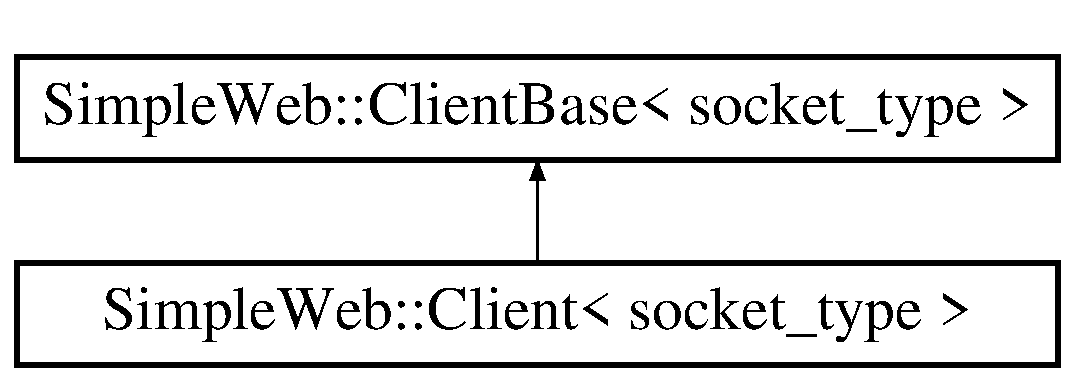
\includegraphics[height=2.000000cm]{a01912}
\end{center}
\end{figure}
\subsection*{Classes}
\begin{DoxyCompactItemize}
\item 
class \hyperlink{a01920}{Config}
\item 
class \hyperlink{a01916}{Response}
\end{DoxyCompactItemize}
\subsection*{Public Member Functions}
\begin{DoxyCompactItemize}
\item 
\mbox{\Hypertarget{a01912_ac8a838ace77f0a1a19b8cb03bdba7e74}\label{a01912_ac8a838ace77f0a1a19b8cb03bdba7e74}} 
std\+::shared\+\_\+ptr$<$ \hyperlink{a01916}{Response} $>$ {\bfseries request} (const std\+::string \&request\+\_\+type, const std\+::string \&path=\char`\"{}/\char`\"{}, boost\+::string\+\_\+ref content=\char`\"{}\char`\"{}, const std\+::map$<$ std\+::string, std\+::string $>$ \&header=std\+::map$<$ std\+::string, std\+::string $>$())
\item 
\mbox{\Hypertarget{a01912_aca6cb17dbea9adf0cf1daf9d1ea70f76}\label{a01912_aca6cb17dbea9adf0cf1daf9d1ea70f76}} 
std\+::shared\+\_\+ptr$<$ \hyperlink{a01916}{Response} $>$ {\bfseries request} (const std\+::string \&request\+\_\+type, const std\+::string \&path, std\+::iostream \&content, const std\+::map$<$ std\+::string, std\+::string $>$ \&header=std\+::map$<$ std\+::string, std\+::string $>$())
\item 
\mbox{\Hypertarget{a01912_ad21735a9bda2fae6aedd811efae981e1}\label{a01912_ad21735a9bda2fae6aedd811efae981e1}} 
void {\bfseries close} ()
\end{DoxyCompactItemize}
\subsection*{Public Attributes}
\begin{DoxyCompactItemize}
\item 
\mbox{\Hypertarget{a01912_af17ddd25319c4f9029969441dfd54eff}\label{a01912_af17ddd25319c4f9029969441dfd54eff}} 
\hyperlink{a01920}{Config} \hyperlink{a01912_af17ddd25319c4f9029969441dfd54eff}{config}
\begin{DoxyCompactList}\small\item\em Set before calling request. \end{DoxyCompactList}\end{DoxyCompactItemize}
\subsection*{Protected Member Functions}
\begin{DoxyCompactItemize}
\item 
\mbox{\Hypertarget{a01912_a4a74d44c9df44d0d469ad453bdac43bf}\label{a01912_a4a74d44c9df44d0d469ad453bdac43bf}} 
{\bfseries Client\+Base} (const std\+::string \&host\+\_\+port, unsigned short default\+\_\+port)
\item 
\mbox{\Hypertarget{a01912_ac511a8e5de870f533f8c28270c82dbfa}\label{a01912_ac511a8e5de870f533f8c28270c82dbfa}} 
std\+::pair$<$ std\+::string, unsigned short $>$ {\bfseries parse\+\_\+host\+\_\+port} (const std\+::string \&host\+\_\+port, unsigned short default\+\_\+port)
\item 
\mbox{\Hypertarget{a01912_a4c1f364a57eaef8fd10c29a82e475010}\label{a01912_a4c1f364a57eaef8fd10c29a82e475010}} 
virtual void {\bfseries connect} ()=0
\item 
\mbox{\Hypertarget{a01912_ab76f469e8f909bf046a80d5afad70469}\label{a01912_ab76f469e8f909bf046a80d5afad70469}} 
std\+::shared\+\_\+ptr$<$ boost\+::asio\+::deadline\+\_\+timer $>$ {\bfseries get\+\_\+timeout\+\_\+timer} (std\+::size\+\_\+t timeout=0)
\item 
\mbox{\Hypertarget{a01912_af11668a7cbf1a4e51f694c853cb70afe}\label{a01912_af11668a7cbf1a4e51f694c853cb70afe}} 
void {\bfseries parse\+\_\+response\+\_\+header} (const std\+::shared\+\_\+ptr$<$ \hyperlink{a01916}{Response} $>$ \&response) const
\item 
\mbox{\Hypertarget{a01912_afa5ddce26ed4c7570a764e2ff003fa25}\label{a01912_afa5ddce26ed4c7570a764e2ff003fa25}} 
std\+::shared\+\_\+ptr$<$ \hyperlink{a01916}{Response} $>$ {\bfseries request\+\_\+read} ()
\item 
\mbox{\Hypertarget{a01912_ae7fa171a9555114e702cafb3f85bc7d5}\label{a01912_ae7fa171a9555114e702cafb3f85bc7d5}} 
void {\bfseries request\+\_\+read\+\_\+chunked} (const std\+::shared\+\_\+ptr$<$ \hyperlink{a01916}{Response} $>$ \&response, boost\+::asio\+::streambuf \&streambuf)
\end{DoxyCompactItemize}
\subsection*{Protected Attributes}
\begin{DoxyCompactItemize}
\item 
\mbox{\Hypertarget{a01912_abe07c05fed46efc9e6aa76736961ae20}\label{a01912_abe07c05fed46efc9e6aa76736961ae20}} 
boost\+::asio\+::io\+\_\+service {\bfseries io\+\_\+service}
\item 
\mbox{\Hypertarget{a01912_a2001dc43f4c3ef1f07a86eea8fbf8082}\label{a01912_a2001dc43f4c3ef1f07a86eea8fbf8082}} 
boost\+::asio\+::ip\+::tcp\+::resolver {\bfseries resolver}
\item 
\mbox{\Hypertarget{a01912_a48b0e61c61cfc3d5307a0101cc30a28e}\label{a01912_a48b0e61c61cfc3d5307a0101cc30a28e}} 
std\+::unique\+\_\+ptr$<$ socket\+\_\+type $>$ {\bfseries socket}
\item 
\mbox{\Hypertarget{a01912_a2c0d5c3d38f4a6a21b67918199b498da}\label{a01912_a2c0d5c3d38f4a6a21b67918199b498da}} 
std\+::mutex {\bfseries socket\+\_\+mutex}
\item 
\mbox{\Hypertarget{a01912_a4436f29ffdce0b29b210cbecd972ffef}\label{a01912_a4436f29ffdce0b29b210cbecd972ffef}} 
std\+::string {\bfseries host}
\item 
\mbox{\Hypertarget{a01912_aadd3336b64a1f8d559af656554ddd0e9}\label{a01912_aadd3336b64a1f8d559af656554ddd0e9}} 
unsigned short {\bfseries port}
\end{DoxyCompactItemize}


The documentation for this class was generated from the following file\+:\begin{DoxyCompactItemize}
\item 
client\+\_\+http.\+hpp\end{DoxyCompactItemize}

\chapter{R\+E\+A\+D\+ME}
\label{a01913}
\Hypertarget{a01913}
\input{a01913}
\chapter{R\+E\+A\+D\+ME}
\label{a01914}
\Hypertarget{a01914}
\input{a01914}
\chapter{update so we can get gcc 6}
\label{a01915}
\Hypertarget{a01915}
apt-\/get -\/y upgrade \&\& apt-\/get -\/y update \&\& apt-\/get install -\/y software-\/properties-\/common \&\& add-\/apt-\/repository ppa\+:ubuntu-\/toolchain-\/r/test \section*{install xacc deps}

apt-\/get -\/y update \&\& apt-\/get install -\/y \$(dpkg --info xacc\+\_\+1.\+0\+\_\+amd64.\+deb $\vert$ grep Depends $\vert$ sed \char`\"{}s/.$\ast$ends\+:\textbackslash{} //\char`\"{} $\vert$ sed \textquotesingle{}s/,//g\textquotesingle{}) git cmake libspdlog-\/dev 
\chapter{R\+E\+A\+D\+ME}
\label{a01916}
\Hypertarget{a01916}
\hypertarget{a01916}{}\section{Simple\+Web\+:\+:Client\+Base$<$ socket\+\_\+type $>$\+:\+:Response Class Reference}
\label{a01916}\index{Simple\+Web\+::\+Client\+Base$<$ socket\+\_\+type $>$\+::\+Response@{Simple\+Web\+::\+Client\+Base$<$ socket\+\_\+type $>$\+::\+Response}}
\subsection*{Public Attributes}
\begin{DoxyCompactItemize}
\item 
\mbox{\Hypertarget{a01916_a77d65a7cac84d8aaa55c0e9ca36e8a2d}\label{a01916_a77d65a7cac84d8aaa55c0e9ca36e8a2d}} 
std\+::string {\bfseries http\+\_\+version}
\item 
\mbox{\Hypertarget{a01916_a9680ebdb0bf18bc448d94dde80b85e0d}\label{a01916_a9680ebdb0bf18bc448d94dde80b85e0d}} 
std\+::string {\bfseries status\+\_\+code}
\item 
\mbox{\Hypertarget{a01916_acac4ceea43b469687c3869211f5d58bb}\label{a01916_acac4ceea43b469687c3869211f5d58bb}} 
std\+::string {\bfseries content\+Type}
\item 
\mbox{\Hypertarget{a01916_a3767341b925b88a56874439169876cd9}\label{a01916_a3767341b925b88a56874439169876cd9}} 
std\+::istream {\bfseries content}
\item 
\mbox{\Hypertarget{a01916_aaff1d7aeb8f3f75c36a6243af50a2616}\label{a01916_aaff1d7aeb8f3f75c36a6243af50a2616}} 
std\+::unordered\+\_\+multimap$<$ std\+::string, std\+::string, \hyperlink{a01904}{case\+\_\+insensitive\+\_\+hash}, \hyperlink{a01900}{case\+\_\+insensitive\+\_\+equals} $>$ {\bfseries header}
\item 
\mbox{\Hypertarget{a01916_a4dd09f31041adcb9f3f75108f6287511}\label{a01916_a4dd09f31041adcb9f3f75108f6287511}} 
int {\bfseries content\+Length}
\end{DoxyCompactItemize}
\subsection*{Friends}
\begin{DoxyCompactItemize}
\item 
\mbox{\Hypertarget{a01916_aee5298660229dd276c7169cf7ef3d387}\label{a01916_aee5298660229dd276c7169cf7ef3d387}} 
class {\bfseries Client\+Base$<$ socket\+\_\+type $>$}
\item 
\mbox{\Hypertarget{a01916_adb9f3938c0e5fcb2b232ca66a7089335}\label{a01916_adb9f3938c0e5fcb2b232ca66a7089335}} 
class {\bfseries Client$<$ socket\+\_\+type $>$}
\end{DoxyCompactItemize}


The documentation for this class was generated from the following file\+:\begin{DoxyCompactItemize}
\item 
client\+\_\+http.\+hpp\end{DoxyCompactItemize}

\chapter{R\+E\+A\+D\+ME}
\label{a01917}
\Hypertarget{a01917}
\input{a01917}
\chapter{R\+E\+A\+D\+ME}
\label{a01918}
\Hypertarget{a01918}
\input{a01918}
\chapter{Fire Data Files}
\label{a01919}
\Hypertarget{a01919}
This directory contains data files that are used for data-\/y things...

Most of these files are for nuclear astrophysics problems on nucleosynthesis in supernovae or other such systems and were originally developed by Mike Guidry at the University of Tennessee. 
\chapter{2016-\/10-\/02-\/about-\/gravity-\/theme}
\label{a01920}
\Hypertarget{a01920}


 layout\+: post title\+: About the Gravity Theme permalink\+: /about/about-\/gravity-\/theme \subsection*{category\+: about }

\subsection*{Gravity}

Minimal, text based, liberal Jekyll theme~\newline
for sharing your awesome ideas.

~\newline
 \begin{center}\end{center} 

\begin{center}{\bfseries Get up and running with Gravity}\end{center} 

\begin{center}\end{center}  ~\newline
   {\bfseries Posting}  

  \begin{DoxyVerb}  - Create a .markdown file inside <code class="highlighter-rouge">_posts</code> folder.<br>
  - Name the file according to the format YY-MM-DD-[short name for your post].<br>  <code>2016-03-30-i-love-design.markdown</code><br>
  - Write the <a href="jekyll">Front Matter</a> and content in the file.<br>
  <div class="example">
    <span class='manual'>FORMAT</span><BR>
    <pre>---
\end{DoxyVerb}
 layout\+: post $\vert$ default $\vert$ page title\+: String Post Title date\+: Time Stamp categories\+: String $\vert$ Array of Strings Category / Categories  ---  

 
\begin{DoxyPre}---
layout: post
title:  "The One with the Blackout"
date:   2016-03-30 19:45:31 +0530
categories: ["life", "friends"]
---\end{DoxyPre}
 

  

~\newline
   {\bfseries Create Pages}  

  \begin{DoxyVerb}  - Create a .md file in the root directory.<br>
  - Name the file with the desired page link name.<br>  <code>about.md</code><br><code>design.md</code><br>
  - Write the <a href="jekyll">Front Matter</a> and content in the file.
  <div class="example">
    <span class='manual'>FORMAT</span><BR>
    <pre>---
\end{DoxyVerb}
 layout\+: page title\+: String Title of the webpage permalink\+: / String / Permalink for the webpage tagline\+: String Optional Gravity Feature \+: Tagline for the page ---  

 
\begin{DoxyPre}---
layout: page
title:  "Science"
permalink:   /science/
tagline : "Humanity is overrated."
---\end{DoxyPre}
 

  

~\newline
   {\bfseries Create Archives/ Category Pages}~\newline
 ~\newline
  

 Introducing {\bfseries Archive Pages}.~\newline


  You can display a list of all the post corresponding to a particular category on a standalone Page using the {\ttfamily \textquotesingle{}archive\textquotesingle{}} layout.   ~\newline




  \begin{DoxyVerb}  - Create a .md file in the root directory.<br>
  - Name the file. Preferred name will be the name of the category<br>  <code>life.md</code><br>
  - Write the <a href="jekyll">Front Matter</a> and content in the file.
  <div class="example">
    <span class='manual'>FORMAT</span><BR>
<pre>---
\end{DoxyVerb}
 layout\+: archive Archive Page Layout title\+: String Title of the webpage permalink\+: / String / Permalink for the webpage tagline\+: String  Tagline for the page category \+: String  Name of the category of which the page will show posts. ---  

 
\begin{DoxyPre}---
layout: archive
title:  "Design"
permalink : "Design"
category: "design"
tagline: "It's all about perception."
---\end{DoxyPre}
 ~\newline
  
\chapter{2016-\/10-\/02-\/fire-\/jekyll-\/configuration}
\label{a01921}
\Hypertarget{a01921}


 layout\+: post title\+: Fire Jekyll Configuration permalink\+: /about/jekyll\+\_\+config \subsection*{category\+: about }

Fire uses Jekyll for publishing documentation on Git\+Hub Pages and it uses the \href{http://hemangsk.github.io/Gravity/}{\tt Gravity theme}. There are several important things to keep in mind for this configuration. The Gemfile should contain


\begin{DoxyCode}
source 'https://rubygems.org'

# Ascii Doctor and PlantUML
gem 'jekyll', '~> 2.5'
gem 'asciidoctor', '~> 1.5'
gem 'coderay', '1.1.0'
gem 'rake-jekyll', '~> 1.0'
gem 'jekyll-plantuml', '~> 1.1' 

group :jekyll\_plugins do
  gem "jekyll-asciidoc"
  gem 'asciidoctor-diagram' 
end
\end{DoxyCode}


I ran into two major problems with Git\+Hub that took hours to fix and then only after contacting Git\+Hub directly.


\begin{DoxyItemize}
\item The site.\+url (or just \char`\"{}url\char`\"{}) and site.\+baseurl variables in \+\_\+config.\+yml must be set to \char`\"{}http\+://\mbox{[}username\mbox{]}.\+github.\+io/\mbox{[}project\mbox{]}\char`\"{} for a project level deployment as in
\end{DoxyItemize}


\begin{DoxyCode}
url = "http://jayjaybillings.github.io"
baseurl = "/fire"
\end{DoxyCode}



\begin{DoxyItemize}
\item The only valid places to put github.\+io files are in the master branch, master/docs or in gh-\/pages. I used gh-\/pages/doc and it would not work until I merged into master/docs.
\end{DoxyItemize}

The Gravity theme works as expected when deployed using


\begin{DoxyCode}
bundle exec jekyll serve
\end{DoxyCode}


but deployment to Git\+Hub fails because the style.\+scss file has references to empty scss files in \+\_\+ssas directory starting at line 47. When these imports are removed or commented out, Git\+Hub will build the site.

\subsection*{Acknowledgements }

Thanks to  for encouraging me to not give up and sharing some expertise. Thanks also to Shawna Jean from Git\+Hub for answering my ticket on a Sunday. 
\chapter{2016-\/10-\/29-\/fire-\/memory-\/model}
\label{a01922}
\Hypertarget{a01922}


 layout\+: post title\+: Memory Model permalink\+: /design/memory\+\_\+model \subsection*{category\+: design }

The memory model in Fire is meant to be simple and efficient. The idea is that sometimes striving for the best performance {\itshape and} the highest architectural purity is stupid and, furthermore, Y\+A\+G\+NI.

Fire takes advantage of the latest updates to C++ and relies heavily on C++11 memory management enhancements to get the best performance.

\section*{Return by Value}

There is no need to return by reference (pointer) for most functions in Fire because it uses C++11. Thus the following code is performs very well\+:


\begin{DoxyCode}
vector<int> getVec() \{
    vector<int> myVec;
    ... \textcolor{comment}{// Some code to fill the vector}
    \textcolor{keywordflow}{return} myVec;
\}

\textcolor{keywordtype}{int} main(\textcolor{keywordtype}{int} argc, \textcolor{keywordtype}{char}** argv) \{
    vector<int> mainVec = getVec();
    \textcolor{keywordflow}{return} EXIT\_SUCCESS;
\}
\end{DoxyCode}


This code would have performed very slowly in earlier versions of C++ because they did not provide so called \char`\"{}move semantics\char`\"{} like C++11. The problem in older versions of C++ comes from the fact that there would be at least two copies the above code. First, my\+Vec is copied into the return value of get\+Vec() when it returns. Second, the return value of get\+Vec() is copied into main\+Vec.

C++11 eliminates the second copy with move semantics. The first copy is eliminated by a process called {\itshape return value optimization,} which is implemented directly by the compiler.

The important implication for this is that functions in Fire can be much simpler and easier to understand while simultaneously performing very well, or, as we like to say with purely technical language, \char`\"{}running like a scalded dog.\char`\"{} ;-\/) This performance is especially important for the build$<$$>$() template, which encapsulates the construction of objects. Without move semantics and return value optimization, it would perform very poorly unless it returned a pointer.

\section*{Public Data}

The proper implementation of a pure, public data structure in Fire is to use a {\itshape struct} instead of a class. It would would look like\+:


\begin{DoxyCode}
\textcolor{keyword}{struct }MyData \{
    \textcolor{keywordtype}{int} A;
    \textcolor{keywordtype}{int} B;
    \textcolor{keyword}{const} \textcolor{keywordtype}{int} C;

    MyData(\textcolor{keywordtype}{int} otherC) : C(otherC) \{\};
\};
\end{DoxyCode}


\subsubsection*{Handling Const Members}

As shown in the example, constructors and initializer lists should be used for {\itshape const} data members. This also means that special care should be taken so that structs do not have a large amount of const-\/qualified members. This makes initialization complicated since const-\/qualified members must be initialized in the initializer list instead of the body of the constructor. In extreme cases it may be necessary to replace a constructor like


\begin{DoxyCode}
MyConstructor(\textcolor{keywordtype}{int} a, \textcolor{keywordtype}{int} b, \textcolor{keywordtype}{int} c,...) : myA(a), myB(b), myC(c), ... \{\};
\end{DoxyCode}


with something like


\begin{DoxyCode}
MyConstructor(\textcolor{keyword}{const} vector<int> & values) : myA(values[0]), myB(values[1]), myC(values[2]), ... \{\};
\end{DoxyCode}


which has the benefit of having a shorter input argument list. This is convenient for line-\/fed data parsed from legacy data formats, as is the case for \hyperlink{a01259}{fire\+::astrophysics\+::\+Species}.

Another possibility is to do something more drastic, like


\begin{DoxyCode}
MyConstructor(\textcolor{keyword}{const} vector<int> & values) : myValues(values), ... \{\};
\end{DoxyCode}


where explicitly defining myA, myB, myC and other members has been replaced with an vector. This is not recommended in the case where the vector contains separately accessed values like myA, myB and myC because it is bad design. However, it is ideal in the case where my\+Values is actually an immutable vector of dense data of a primitive type used for iteration.

If a struct would have so many individual const-\/qualified data members that a vector would be required to initialize it, then it would be better to switch to a class instead, hold the vector data as private state, and provide access via {\itshape accessors.}

\subsubsection*{When to use accessors}

Fire uses structs over classes for small data structures of pure data because, in some cases, {\itshape accessor functions} may be evil. Accessors -\/ or functions that start with \char`\"{}get\char`\"{} or \char`\"{}set\char`\"{} -\/ are used as a means of managing access to or hiding the state of \char`\"{}private\char`\"{} data in a class. (Hiding internal state is called {\itshape encapsulation.}) In a class like the following it is clear that the accessors are just fluff since the get\+A() and set\+A() functions do no other work than provide access to A, B, and C.


\begin{DoxyCode}
\textcolor{keyword}{class }MyData \{
    \textcolor{keywordtype}{int} A;
    \textcolor{keywordtype}{int} B;
    \textcolor{keywordtype}{int} C;
    ... \textcolor{comment}{// More properties!}
\textcolor{keyword}{public}:
    \textcolor{keywordtype}{int} getA() \{\textcolor{keywordflow}{return} A;\};
    \textcolor{keywordtype}{void} setA(\textcolor{keywordtype}{int} otherA) \{A = otherA;\};
    ... \textcolor{comment}{// More get/set functions for B and C }
\};
\end{DoxyCode}


If the get\+A() and set\+A() functions did some extra work or required other information about internal state, then they would be just fine and well warranted. If they do not do any extra work, then encapsulation is completely violated and can no longer be used as an excuse. That is, the internal state is not actually hidden, so it is better to just make them public. Both C and C++ provide the {\itshape struct} construct for defining a data structure with all public members, and it is a better fit here.

There is another important reason for skipping accessors for pure data structures\+: Accessors are a common source of bugs! While these types of bugs will be easily caught by a good unit test, they can be avoided all together by not using accessors where that makes sense.

In the last section, one valid case for accessors was discussed\+: what if a data class with many const-\/qualified members is needed? Accessors are ideal for providing this information because they keep the code succinct\+:


\begin{DoxyCode}
\textcolor{keyword}{class }MyData \{
    \textcolor{keyword}{const} vector<int> myConstValues;
    ... \textcolor{comment}{// More properties!}
\textcolor{keyword}{public}:

    MyData(\textcolor{keyword}{const} vector<int> values) : myConstValues(values) \{\};

    \textcolor{keywordtype}{int} getA() \{\textcolor{keywordflow}{return} vector[8675309];\};
    ... \textcolor{comment}{// More get/set functions for B, C and others  like A.}
\};
\end{DoxyCode}


\section*{Heap-\/\+Allocated Data Arrays}

Fire combines smart pointers and shared pointers for data arrays. Arrays are loaded into shared pointers and passed to functions as raw pointers. The {\itshape free()} and {\itshape delete()} {\bfseries must not be called} on raw pointers in Fire routines because the shared pointers are responsible for the lifecycle of the memory to which the pointer points.

Here\textquotesingle{}s an example for creating arrays of data and using them appropriately in Fire\+:


\begin{DoxyCode}
\textcolor{keywordtype}{int} main() \{
    \textcolor{comment}{// Will be added. Sorry!}
\}
\end{DoxyCode}


\subsubsection*{More details}

The best performance for arrays of data in C++ comes from using raw pointers, which comes with the obvious down side of memory leaks. The smart pointer was invented to get around the latter problem, but that safety comes at the cost of performance. In the case of C++ smart pointers, and the standard shared pointer in particular, the cost is atomic increments and decrements every time the smart pointer is passed to a function. In Fire, smart pointers should be used if a client class is going to be responsible for modifying the existence of an object (create it, delete it, reallocate it, etc.) or needs to know when such an event happens. That is, if a client class is going to participate in the {\itshape memory lifecycle} of an object, then it needs to have the shared pointer. If it does not need to participate in the memory lifecycle, then it is only working with the array and only needs some type of reference to it, for which a raw pointer will work just fine. (Actual references are fine too if they work for your problem.)

This is consistent with guidance from the broader C++11 community, (c.\+f. -\/ \href{http://channel9.msdn.com/Events/GoingNative/GoingNative-2012/C-11-VC-11-and-Beyond}{\tt Herb Sutter\textquotesingle{}s Going Native 2011 talk}), but it does run the risk that some unknowing developer will call delete on a pointer. That risk is acceptable because it is minimized when developers R\+T\+FM. In practice, accidental deallocations have never happened.

C++ references are not broadly used because Fire makes extensive use of templates and references cannot be stored in templated classes. However, as mentioned above, use them if it works.

This strategy has several benefits that can be summed up simply. Combining the two allows Fire to use an exceptionally small amount of memory, provides very fast access to data on the heap and eliminates memory leaks from its own classes. The latter can be witnessed by testing with memory profilers like Valgrind. (N.\+B. -\/ We can not do anything about memory leaks in third party dependencies.) 
\chapter{2016-\/10-\/30-\/parsers}
\label{a01923}
\Hypertarget{a01923}


 layout\+: post title\+: Parsers permalink\+: /design/parsers \subsection*{category\+: design }

Parsers in Fire implement the I\+Parser interface, which can either be implemented through direct interface realization or by using template specialization for local parsers when appropriate.

\subsection*{Local Parsers}

Local Parsers in Fire represent parsers for resources that are on the local machine (i.\+e. -\/ localhost). These can be streams or files, depending on the implementation. Local Parsers implement I\+Local\+Parser or specialize the Local\+Parser$<$T$>$ template.

\subsubsection*{Templated Local Parsers}

Specializations of Local\+Parser$<$T$>$ should be created in the \char`\"{}fire\char`\"{} namespace. See \hyperlink{a00302_source}{astrophysics/\+Species\+Local\+Parser.\+h} for an example.

This is required by the C++ standard. If you do not create your specialization in the \char`\"{}fire\char`\"{} namespace, you will get an error like the following


\begin{DoxyCode}
error: specialization of ‘template<class T> class fire::LocalParser’ in different namespace [-fpermissive]
 class LocalParser<std::vector<Species>> \{
\end{DoxyCode}


\subsubsection*{Delimited Text Parsers}

One special class of parsers are parsers for delimited text, which is dense text with entries of the same type separated by a common {\itshape delimiter,} like a comma, space, or other character. Fire has a special subclass of Local\+Parser, called the Delimited\+Text\+Parser, that should be used for this type of text.

\subsection*{Parsing Simplified}

The simplest way to use a local parser in Fire is to use the parse$<$$>$() template function. If you implemented Local\+Parser$<$T$>$\+::parse() as described above, the you are most likely parsing your file like this


\begin{DoxyCode}
LocalParser<T> parser;
parser.setSource(fileName);
parser.parse();
shared\_ptr<T> myData = parser.getData();
\end{DoxyCode}


or perhaps by using a builder like this


\begin{DoxyCode}
\textcolor{keyword}{auto} parser = build<LocalParser<vector<T>>, \textcolor{keyword}{const} \textcolor{keywordtype}{string} &>(fileName);
parser.parse();
\textcolor{keyword}{auto} myData = speciesParser.getData();
\end{DoxyCode}


Both of those are great, but you can get the same function in Fire using parse$<$T$>$() as follows


\begin{DoxyCode}
\textcolor{keyword}{auto} myData = parse<T>(filename);
\end{DoxyCode}


In this case, the parse$<$T$>$() function will automatically create the parser and return your data using a Local\+Parser$<$T$>$ if it is available. parse$<$T$>$() is specifically designed for returning vectors of type T from local files. It isn\textquotesingle{}t a substitute for complex parsers, but it saves a lot of effort for regular, block-\/structured data. 
\chapter{2016-\/10-\/30-\/tests}
\label{a01924}
\Hypertarget{a01924}
\hypertarget{a01924}{}\section{Simple\+Web\+:\+:Client$<$ H\+T\+TP $>$ Class Template Reference}
\label{a01924}\index{Simple\+Web\+::\+Client$<$ H\+T\+T\+P $>$@{Simple\+Web\+::\+Client$<$ H\+T\+T\+P $>$}}
Inheritance diagram for Simple\+Web\+:\+:Client$<$ H\+T\+TP $>$\+:\begin{figure}[H]
\begin{center}
\leavevmode
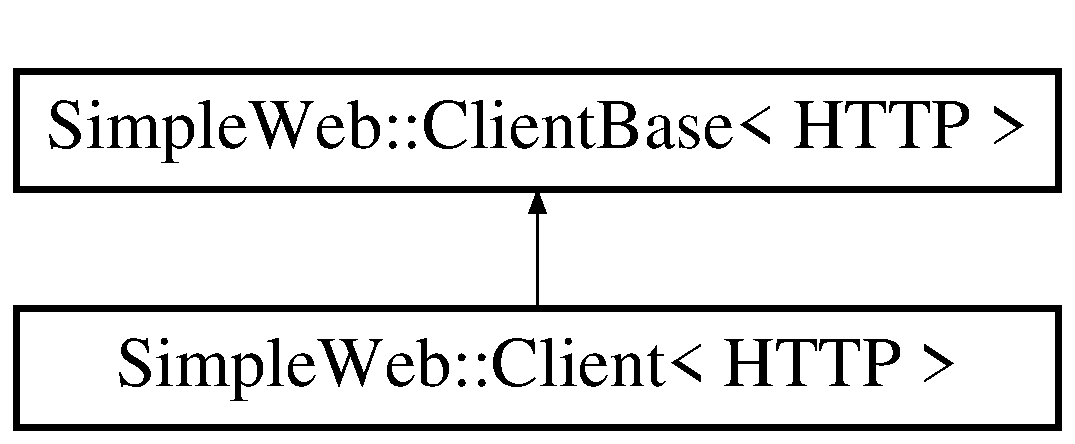
\includegraphics[height=2.000000cm]{a01924}
\end{center}
\end{figure}
\subsection*{Public Member Functions}
\begin{DoxyCompactItemize}
\item 
\mbox{\Hypertarget{a01924_a47655afc849e459096743876391dae17}\label{a01924_a47655afc849e459096743876391dae17}} 
{\bfseries Client} (const std\+::string \&server\+\_\+port\+\_\+path)
\end{DoxyCompactItemize}
\subsection*{Protected Member Functions}
\begin{DoxyCompactItemize}
\item 
\mbox{\Hypertarget{a01924_aebed110274c94b539e2d0a857c24991d}\label{a01924_aebed110274c94b539e2d0a857c24991d}} 
void {\bfseries connect} ()
\end{DoxyCompactItemize}
\subsection*{Additional Inherited Members}


The documentation for this class was generated from the following file\+:\begin{DoxyCompactItemize}
\item 
client\+\_\+http.\+hpp\end{DoxyCompactItemize}

\chapter{2016-\/11-\/06-\/astrophysical-\/reactions}
\label{a01925}
\Hypertarget{a01925}


 layout\+: post title\+: Nuclear Reactions in Astrophysical Systems permalink\+: /science/astrophysics/reactions \subsection*{category\+: science }

\section*{Overview}

The astrophysics module of Fire contains a set of classes for managing thermonuclear reactions in astrophysical problems. The Reaction\+Network class is responsible for organizing the species and rates that drive the evolution of the network.

\section*{Configuring the Network}

\section*{Reaction Rates}

Reaction rates are computed using parameterized rates from the R\+E\+A\+C\+L\+IB rate library. The R\+E\+A\+C\+L\+IB rates are parameterized by seven coefficients and can be computed as

The rate is computed as

\$\$ R = p\+\_\+s$\ast$ R\+\_\+k \$\$

where \$\$p\+\_\+s\$\$ is the prefactor (based on the statistical prefactor) and

\$\$ R\+\_\+k = (p\+\_\+1 + \{p\+\_\+2\}\{T\+\_\+9\} + \{p\+\_\+3\}\{T\+\_\+9$^\wedge$\{1/3\}\} + p\+\_\+\{4\}T\+\_\+9$^\wedge$\{1/3\}
\begin{DoxyItemize}
\item p\+\_\+\{5\}T\+\_\+9 + p\+\_\+\{6\}T\+\_\+9$^\wedge$\{5/3\} + p\+\_\+\{7\} T\+\_\+9) \$\$
\end{DoxyItemize}

\$\$\+T\+\_\+9\$\$ is the the temperature in units of \$\$10$^\wedge$9\$\$ Kelvin. The prefactor is given by

\$\$ p\+\_\+s = s$^\wedge$\{(n\+\_\+R -\/1)\}. \$\$

where \$\$s\$\$ is the statistical factor (an input from R\+E\+A\+C\+L\+IB), \$\$\$\$ is the density in units of \$\$10$^\wedge$8 \{g\}\{m$^\wedge$3\}\$\$ and \$\$n\+\_\+R\$\$ is the number of reactants in the reaction (species on the left hand side that start the reaction).

In general k may be greater than 1 in the summation for the rate, but in this work k = 1 and \$\$R = R\+\_\+k\$\$.

More information on how this library is parsed is available in the documentation for \href{{{ site.baseurl }}}{\tt the Reaction A\+S\+C\+II format}.

\subsubsection*{Some Design Problems}

Some of the code in the astrophysics module was adapted from an older code called the Fast Explicit Reaction Network (F\+E\+RN) solver. F\+E\+RN is a research code that was developed by students and others at the University of Tennessee to explore issues around efficiently solving reaction networks using advanced methods and hardware.

F\+E\+RN has a very low-\/level design with significant flaws. The routines in F\+E\+RN that initialize the network pack everything into arrays with little regard for treating the memory right, among other problems. When this code was ported to Fire, the memory errors were fixed, but the larger considerations for a cleaner design were not addressed. These problems are discussed in-\/line in the classes themselves and will be addressed in a future release.

\section*{References}

\char`\"{}\+Stars and Stellar Processes\char`\"{}, Mike Guidry, to be published Cambridge University Press. 
\chapter{2016-\/11-\/12-\/astrophysics-\/reactions-\/ascii-\/format}
\label{a01926}
\Hypertarget{a01926}


 layout\+: post title\+: Astrophysics Reactions A\+S\+C\+II File Format permalink\+: /science/astrophysics/reactions-\/ascii-\/format \subsection*{category\+: science }

Simulations of thermonuclear networks in astrophysics require lists of reactions that describe how the species evolve over time. Fire supports a legacy A\+S\+C\+II format with a 8-\/line specification for a reaction. Each entry in each line is separated by a space. See \hyperlink{a00290_source}{Reaction.\+h} for full details on each required value.

The first line for each reaction contains\+:


\begin{DoxyItemize}
\item Name/\+Label -\/ A string of the form \char`\"{}he4+he4+he4-\/-\/$>$c12\char`\"{} that describes the reaction.
\item Reaction Group Class -\/ an integer
\item Reaction Group Index -\/ an integer
\item R\+E\+A\+C\+L\+IB Class -\/ an integer
\item Number of reacting species -\/ an integer
\item Number of resulting products -\/ an integer
\item Electron capture flag -\/ a bool
\item Reverse reaction flag -\/ a bool
\item Statistical factor -\/ a double
\item Energy release -\/ a double
\end{DoxyItemize}

The second line contains the seven rate coefficients from the R\+E\+A\+C\+L\+IB library, all doubles. The third line contains the array of atomic numbers for the reactants in this reaction, which are integers. The fourth, fifth, and sixth lines are also integers for the reactant neutron number and product atomic and neutron numbers. Each of these four lines has one integer for each reactant and product in the system, but with no more than four entries per line. (See example below for more details.)

The seventh and eighth lines contain quantities that are used for {\itshape Partial Equilibrium} approximations. Each line contains up to three integers.


\begin{DoxyCode}
he4+he4+he4-->c12 3 0 8 3 1 0 0 0.16666667 7.27500
-24.99350000 -4.29702000 -6.69304000 15.59030000 -1.57387000 0.17058800 -9.02800000
2 2 2 // Since numReactants = 3 and he4 has Z=2, there are three values on this line equal to 2.
2 2 2 // Same, but for he4's neutron number
6 // There is only one product and Z=6 for C12.
6 // N=6 for C12
0 0 0 
1 
ne20-->he4+o16 2 3 2 1 2 0 1 1.00000000 -4.73400
109.31000000 -72.75840000 293.66400000 -384.97400000 20.23800000 -1.00379000 201.19300000
10 // Z for ne20
10 // N for ne20
2 8 // Z for he4 and o16
2 8 // N for he4 and o16
3 
0 2 
\end{DoxyCode}
 
\chapter{2016-\/11-\/12-\/astrophysics-\/species-\/ascii-\/format}
\label{a01927}
\Hypertarget{a01927}


 layout\+: post title\+: Astrophysics Species A\+S\+C\+II File Format permalink\+: /science/astrophysics/species-\/ascii-\/format \subsection*{category\+: science }

Simulations of thermonuclear networks in astrophysics require lists of species that react with each other. Fire supports a legacy A\+S\+C\+II format with a 4-\/line specification for a species. See \hyperlink{a00299_source}{Species.\+h} for ful details on each required value.

The first line specifies the


\begin{DoxyItemize}
\item species name -\/ a string
\item mass number -\/ an integer
\item atomic number -\/ an integer
\item neutron number -\/ an integer
\item mass fraction -\/ a double
\item mass excess -\/ a double
\end{DoxyItemize}

The second through fourth lines specify parameters for the partition function. Each line contains eight double precision numbers separated by spaces.

Here is a sample for 4\+He and 12C.


\begin{DoxyCode}
4He 4 2 2 0.0 2.425
1.0 1.0 1.0 1.0 1.0 1.0 1.0 1.0
1.0 1.0 1.0 1.0 1.0 1.0 1.0 1.0
1.0 1.0 1.0 1.0 1.0 1.0 1.0 1.0
12C 12 6 6 0.0416666 0.0
1.0 1.0 1.0 1.0 1.0 1.0 1.0 1.0
1.0 1.0 1.0 1.0 1.0 1.0 1.0 1.0
1.0 1.0 1.0 1.0 1.0 1.0 1.0 1.0
\end{DoxyCode}
 
\chapter{2016-\/11-\/13-\/\+Notes-\/\+On-\/\+Getting-\/\+Eclipse-\/\+To-\/\+Work}
\label{a01928}
\Hypertarget{a01928}
\hypertarget{a01928}{}\section{Simple\+Web\+:\+:Client$<$ H\+T\+T\+PS $>$ Class Template Reference}
\label{a01928}\index{Simple\+Web\+::\+Client$<$ H\+T\+T\+P\+S $>$@{Simple\+Web\+::\+Client$<$ H\+T\+T\+P\+S $>$}}
Inheritance diagram for Simple\+Web\+:\+:Client$<$ H\+T\+T\+PS $>$\+:\begin{figure}[H]
\begin{center}
\leavevmode
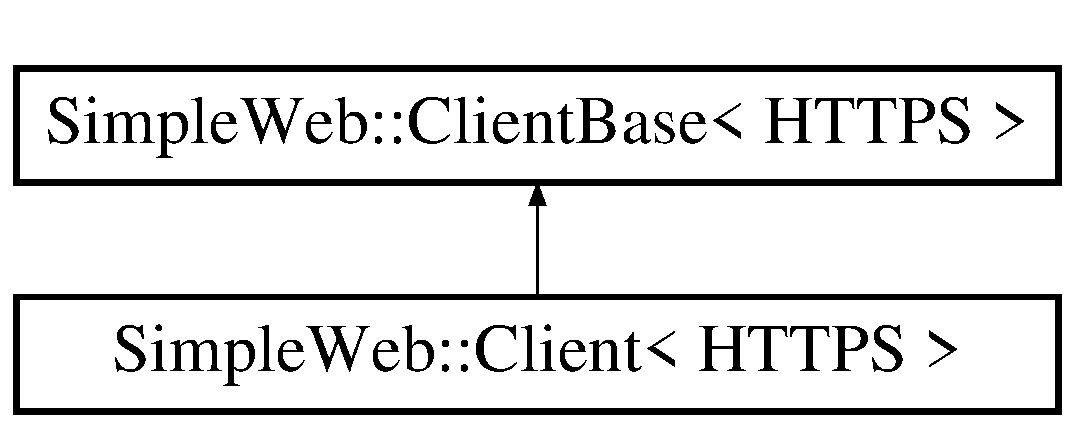
\includegraphics[height=2.000000cm]{a01928}
\end{center}
\end{figure}
\subsection*{Public Member Functions}
\begin{DoxyCompactItemize}
\item 
\mbox{\Hypertarget{a01928_abd87d3dc08c9fed3a60f18c749b8bacd}\label{a01928_abd87d3dc08c9fed3a60f18c749b8bacd}} 
{\bfseries Client} (const std\+::string \&server\+\_\+port\+\_\+path, bool verify\+\_\+certificate=true, const std\+::string \&cert\+\_\+file=std\+::string(), const std\+::string \&private\+\_\+key\+\_\+file=std\+::string(), const std\+::string \&verify\+\_\+file=std\+::string())
\end{DoxyCompactItemize}
\subsection*{Protected Member Functions}
\begin{DoxyCompactItemize}
\item 
\mbox{\Hypertarget{a01928_a833f6fd136e3158b873bee024d6e188c}\label{a01928_a833f6fd136e3158b873bee024d6e188c}} 
void {\bfseries connect} ()
\end{DoxyCompactItemize}
\subsection*{Protected Attributes}
\begin{DoxyCompactItemize}
\item 
\mbox{\Hypertarget{a01928_afe57679cc6153d5d1fe8abc94a8fa58a}\label{a01928_afe57679cc6153d5d1fe8abc94a8fa58a}} 
boost\+::asio\+::ssl\+::context {\bfseries context}
\end{DoxyCompactItemize}
\subsection*{Additional Inherited Members}


The documentation for this class was generated from the following file\+:\begin{DoxyCompactItemize}
\item 
client\+\_\+https.\+hpp\end{DoxyCompactItemize}

\chapter{2016-\/11-\/14-\/builders}
\label{a01929}
\Hypertarget{a01929}


 layout\+: post title\+: Builders permalink\+: /design/builders \subsection*{category\+: design }

Objects in Fire should be constructed using developer-\/provided specializations of the build$<$T$>$() template function, which is described in \hyperlink{a00368_source}{build.\+h}.

Object construction can be problematic in software projects if the method of initializing those objects changes. For example, it may be sufficient to initialize an object with the following\+:


\begin{DoxyCode}
MyCustomClass object; \textcolor{comment}{// Nullary constructor}
MyCustomClass copiedObject(\textcolor{keywordtype}{object}); \textcolor{comment}{// Copy constructor}
MyCustomClass otherObject(5); \textcolor{comment}{// Special constructor that does something else.}
\end{DoxyCode}


What happens if the design of {\itshape My\+Custom\+Class} changes so that a special {\itshape initialize} operation must be called after the constructor? Or what if data members need to be filled? Then initialization would look like this\+:


\begin{DoxyCode}
MyCustomClass object(5); \textcolor{comment}{// Pass a special argument}
\textcolor{keywordtype}{object}.setX(x); \textcolor{comment}{// Set some data}
\textcolor{keywordtype}{object}.setY(y);
\textcolor{keywordtype}{object}.init(); \textcolor{comment}{// Initialize the object for some long-running work after construction}
\end{DoxyCode}


This quickly becomes troublesome if {\itshape My\+Custom\+Class} is used in many places because it requires a lot of code and could lead to bugs. Thus, Fire uses a templated \char`\"{}builder\char`\"{} function to construct objects like so


\begin{DoxyCode}
\textcolor{keyword}{auto} \textcolor{keywordtype}{object} = build<MyCustomClass>(); \textcolor{comment}{// Default construction}
\textcolor{keyword}{auto} otherObject = build<MyCustomClass>(5,x,y); \textcolor{comment}{// Initialized with data}
\end{DoxyCode}


where the build$<$T$>$() template is specialized by the developer specifically for constructing My\+Custom\+Class in appropriate ways. This eliminates the details of exactly how My\+Custom\+Class is constructed and additionally avoids the \char`\"{}pollution\char`\"{} of duplicating the code to construct My\+Custom\+Class every it is used. Different versions of build$<$T$>$() exist, including versions for instantiation by lists and other input arguments; both versions in the code sample above are valid.

The cleanest way to provide specializations of build$<$T$>$() for any class is after the class in the header file where the class is defined.

The build$<$T$>$() template function is currently defined in \hyperlink{a00368_source}{build.\+h} in the parsers module, but may move in the future.

\subsection*{Example}

The \hyperlink{a00290_source}{Reaction.\+h} file in the astrophysics module has a good examples of providing a specialization of build$<$T$>$(). The only catch is that build$<$T$>$() specializations must be created in the {\itshape fire} namespace, not a subspace.

\hyperlink{a00302_source}{Species\+Local\+Parser.\+h} shows a good example of \char`\"{}implicit instantiation\char`\"{} for the build$<$T$>$() function for the Species class. In this case, the compiler automatically creates the specialized version of build$<$T$>$() based on type inference and the second version of build$<$T$>$() in \hyperlink{a00368_source}{build.\+h}.

\subsection*{build$<$T$>$() vs parse$<$T$>$()}

In some cases the build$<$T$>$() can be grammatically cumbersome. Consider the following example\+:


\begin{DoxyCode}
\textcolor{keyword}{auto} parser = build<LocalParser<vector<T>>, \textcolor{keyword}{const} \textcolor{keywordtype}{string} &>(fileName);
parser.parse();
\textcolor{keyword}{auto} myData = speciesParser.getData();
\end{DoxyCode}


The problem with this code is that it is essentially the same thing as what build$<$T$>$() is meant to prevent -\/ bloat that will be copied everywhere! The worst part of the bloat is the template arguments, which are most likely constant across many different parsers. It is better to use parse$<$T$>$() in cases like this, which looks like the following\+:


\begin{DoxyCode}
\textcolor{keyword}{auto} myData = parse<T>(filename);
\end{DoxyCode}


parse$<$T$>$() is specifically designed for returning vectors of type T from local files. It isn\textquotesingle{}t a substitute for complex parsers, but it saves a lot of effort for regular, block-\/structured data.

The two major differences between these two methods are


\begin{DoxyItemize}
\item Code cleanliness
\item parse$<$T$>$() automatically parses the file, whereas build$<$T$>$() probably does and should not.
\end{DoxyItemize}

The second point is really important. Should your build$<$T$>$() parse as well as build? That\textquotesingle{}s a design issue that we\textquotesingle{}ll defer for now, but keep in mind that if your build$<$T$>$() routine parses, then your clients should not use parse$<$T$>$() because it calls build$<$T$>$() too, which means your data will be loaded twice into the same array! This is the reason that default build$<$T$>$() implementations for local parsers in Fire {\bfseries never} call parser.\+parse().

\subsubsection*{Author note}

Note\+: Ideally the default version of build would work for variadic template and function arguments, but at the specific function must be implemented. 
\chapter{2016-\/11-\/21-\/solving-\/problems}
\label{a01930}
\Hypertarget{a01930}


 layout\+: post title\+: Solving Problems permalink\+: /science/solving-\/problems \subsection*{category\+: science }

\section*{T\+H\+E\+SE A\+RE N\+O\+T\+ES}

Nothing good here. Just trying to sketch some things out.

\char`\"{}\+Systems\char`\"{} are systems of partial or ordinary differential equations.

\char`\"{}\+Solvers\char`\"{} are routines for factorizing matrices.

\char`\"{}\+Methods\char`\"{} are methods used for solving partial differential equations including finite difference, finite element, particle and other types.

Most codes make no distinction between these three classes, but Fire does because the flexibility afforded by such a distinction is very valuable. Such a distinction makes it possible to modify each class separately without interfering with the others. This means that if the description of the P\+D\+Es change, it will not affect the method that solves those P\+D\+Es or the factorization routines used to solve the matrix.

\subsubsection*{Systems}


\begin{DoxyItemize}
\item R\+HS data
\item L\+HS Operators
\item Boundary Conditions -\/ Can this work if the geometry/mesh is not known at this point? Do we need to have separate F\+E/\+FD System subclasses?
\item Initial Conditions -\/ Same.
\item Method
\end{DoxyItemize}

{\bfseries Problems}


\begin{DoxyItemize}
\item If my Method owns my discretization, what does a System really mean?
\item How do boundary conditions work? They would typically be defined on the boundaries of the mesh, but as defined the system knows nothing about that.
\end{DoxyItemize}

\subsubsection*{Methods}


\begin{DoxyItemize}
\item Geometry
\item Mesh
\item Grid
\end{DoxyItemize}

All this stuff is optional depending on the method type

\section*{None of this is a great idea to me.}
\chapter{about}
\label{a01931}
\Hypertarget{a01931}


 layout\+: page title \+: About \subsection*{permalink\+: /about/ }



 \{\% for post in site.\+categories.\+about \%\}  $<$time datetime=\char`\"{}\{\{ post.\+date $\vert$ date\+\_\+to\+\_\+xmlschema \}\}\char`\"{} itemprop=\char`\"{}date\+Published\char`\"{}$>$\{\{ post.\+date $\vert$ date\+: \char`\"{}\%b \%-\/d, \%\+Y\char`\"{} \}\}$<$/time$>$   \{\{post.\+tag\}\}  ~\newline
  \href{{{site.url}}{{site.baseurl}}{{post.url}}}{\tt \{\{post.\+title\}\}}   \{\{ post.\+content $\vert$ strip\+\_\+html $\vert$ truncatewords\+:20\}\}   \{\% endfor \%\}  
\chapter{design}
\label{a01932}
\Hypertarget{a01932}
\hypertarget{a01932}{}\section{Simple\+Web\+:\+:Server$<$ socket\+\_\+type $>$ Class Template Reference}
\label{a01932}\index{Simple\+Web\+::\+Server$<$ socket\+\_\+type $>$@{Simple\+Web\+::\+Server$<$ socket\+\_\+type $>$}}
Inheritance diagram for Simple\+Web\+:\+:Server$<$ socket\+\_\+type $>$\+:\begin{figure}[H]
\begin{center}
\leavevmode
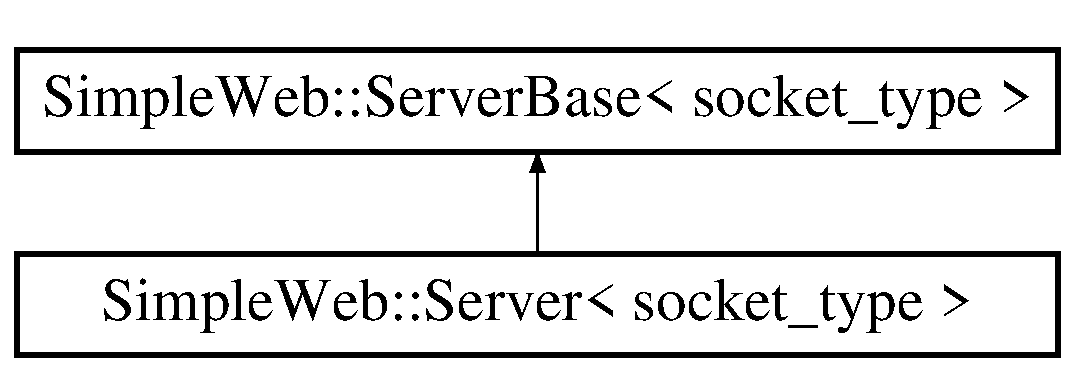
\includegraphics[height=2.000000cm]{a01932}
\end{center}
\end{figure}
\subsection*{Additional Inherited Members}


The documentation for this class was generated from the following file\+:\begin{DoxyCompactItemize}
\item 
server\+\_\+http.\+hpp\end{DoxyCompactItemize}

\chapter{Gravity}
\label{a01933}
\Hypertarget{a01933}
If there\textquotesingle{}s any issue you are facing in setting up this theme I\textquotesingle{}m there for you. Just create an issue in this repository (\href{http://github.com/hemangsk/Gravity}{\tt http\+://github.\+com/hemangsk/\+Gravity}), (\href{https://help.github.com/articles/creating-an-issue/}{\tt https\+://help.\+github.\+com/articles/creating-\/an-\/issue/}) and I\textquotesingle{}ll get back to you asap.



  





 
\chapter{science}
\label{a01934}
\Hypertarget{a01934}


 layout\+: archive title\+: Science permalink\+: /science/ tagline\+: \char`\"{}\+The science behind Fire.\char`\"{} \subsection*{category\+: \char`\"{}science\char`\"{} }
\chapter{Fire Framework}
\label{a01935}
\Hypertarget{a01935}
Fire is a framework for scientific computing. It includes various reusable tools and utilities. This includes
\begin{DoxyItemize}
\item parsers
\item steppers
\end{DoxyItemize}

It also includes domain-\/specific classes for nuclear reaction network simulations in nuclear astrophysics.

\subsection*{Documentation}

Documentation in Fire is generated via Doxygen by running \char`\"{}make doc\char`\"{} during the build. The documentation is viewable \href{http://www.jayjaybillings.com/fire}{\tt online}. The full A\+PI documentation is available at \href{http://www.jayjaybillings.com/fire/api/html/}{\tt the A\+PI reference page}.

You can run \char`\"{}make doc\char`\"{} from build directory to generate the A\+PI documentation. Doxygen handles most of the required documentation without developer intervention. This means that in some cases there may be classes that seem to have minimal documentation in the source, like classes that implement interfaces and provide no additional functionality, but are in fact quite well documented by Doxygen. Most I\+D\+Es will also auto-\/generate descriptions for developers too, so the author(s) see no need to cover every piece of code with comments.

\subsection*{Prerequisites}

You will need git and cmake to build Fire.

\subsection*{Checkout and build}

From a shell, execute the following commands to compile the code\+:


\begin{DoxyCode}
git clone https://github.com/jayjaybillings/fire
mkdir fire-build
cd fire-build
cmake ../fire -DCMAKE\_BUILD\_TYPE=Debug -G"Eclipse CDT4 - Unix Makefiles" -DCMAKE\_ECLIPSE\_VERSION=4.5
make
\end{DoxyCode}


If you would like to use M\+A\+G\+MA for solvers, you need to modify the cmake argument with the path to the M\+A\+G\+MA installation. Your configuration statement should look like the following\+:


\begin{DoxyCode}
cmake ../fire -DCMAKE\_BUILD\_TYPE=Debug -G"Eclipse CDT4 - Unix Makefiles" -DCMAKE\_ECLIPSE\_VERSION=4.5
       MAGMA\_ROOT=/usr/local/lib
\end{DoxyCode}


The above will get the code running, but it will not run the tests or generate the documentation. Issue the following commands to do that\+: 
\begin{DoxyCode}
make test
make doc
\end{DoxyCode}


Build flags, such as -\/\+Wall, can be set by prepending the C\+X\+X\+\_\+\+F\+L\+A\+GS variable to the cmake command as such


\begin{DoxyCode}
CXX\_FLAGS='-Wall' cmake ../fire -DCMAKE\_BUILD\_TYPE=Debug -G"Eclipse CDT4 - Unix Makefiles"
       -DCMAKE\_ECLIPSE\_VERSION=4.5
\end{DoxyCode}


Optimization flags should be handled by setting -\/\+D\+C\+M\+A\+K\+E\+\_\+\+B\+U\+I\+L\+D\+\_\+\+T\+Y\+PE=Release instead of Debug. Likewise, an optimized build with debug information can be acheived by setting -\/\+D\+C\+M\+A\+K\+E\+\_\+\+B\+U\+I\+L\+D\+\_\+\+T\+Y\+PE=Rel\+With\+Debug\+Info.

\subsection*{License}

See the L\+I\+C\+E\+N\+SE file licensing and copyright information. In short, 3-\/clause B\+SD.

\subsection*{Questions}

Questions can be directed to me at jayjaybillings $<$at$>$ gmail $<$dot$>$ com. 
\chapter{Note on Licenses for Third Party Libraries}
\label{a01936}
\Hypertarget{a01936}
This directory holds the Third Party Libraries (T\+P\+Ls) that are used by Fire. Each directory contains the original distribution of the T\+PL as well as a V\+E\+R\+S\+I\+O\+N.\+txt file that describes the version and source for the T\+PL. This extra file also describes where the copyright and license for the T\+PL can be found. Finally, it also contains a C\+Make\+Lists.\+txt if necessary. 
\chapter{simpleini}
\label{a01937}
\Hypertarget{a01937}
A cross-\/platform library that provides a simple A\+PI to read and write I\+N\+I-\/style configuration files. It supports data files in A\+S\+C\+II, M\+B\+CS and Unicode. It is designed explicitly to be portable to any platform and has been tested on Windows, Win\+CE and Linux. Released as open-\/source and free using the M\+IT licence.

\section*{Feature Summary}


\begin{DoxyItemize}
\item M\+IT Licence allows free use in all software (including G\+PL and commercial)
\item multi-\/platform (Windows 95/98/\+M\+E/\+N\+T/2\+K/\+X\+P/2003, Windows CE, Linux, Unix)
\item loading and saving of I\+N\+I-\/style configuration files
\item configuration files can have any newline format on all platforms
\item liberal acceptance of file format
\begin{DoxyItemize}
\item key/values with no section
\item removal of whitespace around sections, keys and values
\end{DoxyItemize}
\item support for multi-\/line values (values with embedded newline characters)
\item optional support for multiple keys with the same name
\item optional case-\/insensitive sections and keys (for A\+S\+C\+II characters only)
\item saves files with sections and keys in the same order as they were loaded
\item preserves comments on the file, section and keys where possible.
\item supports both char or wchar\+\_\+t programming interfaces
\item supports both M\+B\+CS (system locale) and U\+T\+F-\/8 file encodings
\item system locale does not need to be U\+T\+F-\/8 on Linux/\+Unix to load U\+T\+F-\/8 file
\item support for non-\/\+A\+S\+C\+II characters in section, keys, values and comments
\item support for non-\/standard character types or file encodings via user-\/written converter classes
\item support for adding/modifying values programmatically
\item compiles cleanly in the following compilers\+:
\begin{DoxyItemize}
\item Windows/\+V\+C6 (warning level 3)
\item Windows/\+V\+C.\+N\+ET 2003 (warning level 4)
\item Windows/\+VC 2005 (warning level 4)
\item Linux/gcc (-\/\+Wall)
\item Windows/\+Min\+GW G\+CC
\end{DoxyItemize}
\end{DoxyItemize}

\section*{Documentation}

Full documentation of the interface is available in doxygen format.

\section*{Examples}

These snippets are included with the distribution in the file snippets.\+cpp.

\subsubsection*{S\+I\+M\+P\+LE U\+S\+A\+GE}


\begin{DoxyCode}
\{c++\}
CSimpleIniA ini;
ini.SetUnicode();
ini.LoadFile("myfile.ini");
const char * pVal = ini.GetValue("section", "key", "default");
ini.SetValue("section", "key", "newvalue");
\end{DoxyCode}


\subsubsection*{L\+O\+A\+D\+I\+NG D\+A\+TA}


\begin{DoxyCode}
\{c++\}
// load from a data file
CSimpleIniA ini(a\_bIsUtf8, a\_bUseMultiKey, a\_bUseMultiLine);
SI\_Error rc = ini.LoadFile(a\_pszFile);
if (rc < 0) return false;

// load from a string
std::string strData;
rc = ini.LoadData(strData.c\_str(), strData.size());
if (rc < 0) return false;
\end{DoxyCode}


\subsubsection*{G\+E\+T\+T\+I\+NG S\+E\+C\+T\+I\+O\+NS A\+ND K\+E\+YS}


\begin{DoxyCode}
\{c++\}
// get all sections
CSimpleIniA::TNamesDepend sections;
ini.GetAllSections(sections);

// get all keys in a section
CSimpleIniA::TNamesDepend keys;
ini.GetAllKeys("section-name", keys);
\end{DoxyCode}


\subsubsection*{G\+E\+T\+T\+I\+NG V\+A\+L\+U\+ES}


\begin{DoxyCode}
\{c++\}
// get the value of a key
const char * pszValue = ini.GetValue("section-name", 
    "key-name", NULL /*default*/);

// get the value of a key which may have multiple 
// values. If bHasMultipleValues is true, then just 
// one value has been returned
bool bHasMultipleValues;
pszValue = ini.GetValue("section-name", "key-name", 
    NULL /*default*/, &amp;bHasMultipleValues);

// get all values of a key with multiple values
CSimpleIniA::TNamesDepend values;
ini.GetAllValues("section-name", "key-name", values);

// sort the values into the original load order
values.sort(CSimpleIniA::Entry::LoadOrder());

// output all of the items
CSimpleIniA::TNamesDepend::const\_iterator i;
for (i = values.begin(); i != values.end(); ++i) \{ 
    printf("key-name = '%s'\(\backslash\)n", i->pItem);
\}
\end{DoxyCode}


\subsubsection*{M\+O\+D\+I\+F\+Y\+I\+NG D\+A\+TA}


\begin{DoxyCode}
\{c++\}
// adding a new section
rc = ini.SetValue("new-section", NULL, NULL);
if (rc < 0) return false;
printf("section: %s\(\backslash\)n", rc == SI\_INSERTED ? 
    "inserted" : "updated");

// adding a new key ("new-section" will be added 
// automatically if it doesn't already exist)
rc = ini.SetValue("new-section", "new-key", "value");
if (rc < 0) return false;
printf("key: %s\(\backslash\)n", rc == SI\_INSERTED ? 
    "inserted" : "updated");

// changing the value of a key
rc = ini.SetValue("section", "key", "updated-value");
if (rc < 0) return false;
printf("key: %s\(\backslash\)n", rc == SI\_INSERTED ? 
    "inserted" : "updated");
\end{DoxyCode}


\subsubsection*{D\+E\+L\+E\+T\+I\+NG D\+A\+TA}


\begin{DoxyCode}
\{c++\}
// deleting a key from a section. Optionally the entire
// section may be deleted if it is now empty.
ini.Delete("section-name", "key-name", 
    true /*delete the section if empty*/);

// deleting an entire section and all keys in it
ini.Delete("section-name", NULL);
\end{DoxyCode}


\subsubsection*{S\+A\+V\+I\+NG D\+A\+TA}


\begin{DoxyCode}
\{c++\}
// save the data to a string
rc = ini.Save(strData);
if (rc < 0) return false;

// save the data back to the file
rc = ini.SaveFile(a\_pszFile);
if (rc < 0) return false;
\end{DoxyCode}
 
\chapter{R\+E\+A\+D\+ME}
\label{a01938}
\Hypertarget{a01938}
\input{a01938}
\chapter{R\+E\+A\+D\+ME}
\label{a01939}
\Hypertarget{a01939}
\input{a01939}
\chapter{Namespace Index}
\section{Namespace List}
Here is a list of all documented namespaces with brief descriptions\+:\begin{DoxyCompactList}
\item\contentsline{section}{\hyperlink{a00822}{fire} }{\pageref{a00822}}{}
\item\contentsline{section}{\hyperlink{a00826}{rapidjson} \\*Main Rapid\+J\+S\+ON namespace }{\pageref{a00826}}{}
\item\contentsline{section}{\hyperlink{a00828}{Simple\+Web} }{\pageref{a00828}}{}
\end{DoxyCompactList}

\chapter{Hierarchical Index}
\section{Class Hierarchy}
This inheritance list is sorted roughly, but not completely, alphabetically\+:\begin{DoxyCompactList}
\item \contentsline{section}{xacc\+:\+:Accelerator\+Bit}{\pageref{a01095}}{}
\item \contentsline{section}{xacc\+:\+:Accelerator\+Buffer}{\pageref{a01099}}{}
\begin{DoxyCompactList}
\item \contentsline{section}{xacc\+:\+:quantum\+:\+:Simulated\+Qubits}{\pageref{a01083}}{}
\end{DoxyCompactList}
\item \contentsline{section}{xacc\+:\+:Algorithm\+Generator}{\pageref{a01119}}{}
\begin{DoxyCompactList}
\item \contentsline{section}{xacc\+:\+:quantum\+:\+:Inverse\+Q\+FT}{\pageref{a00979}}{}
\item \contentsline{section}{xacc\+:\+:quantum\+:\+:Q\+FT}{\pageref{a00983}}{}
\end{DoxyCompactList}
\item A\+S\+T\+Consumer\begin{DoxyCompactList}
\item \contentsline{section}{xacc\+:\+:quantum\+:\+:Scaffold\+A\+S\+T\+Consumer}{\pageref{a00931}}{}
\end{DoxyCompactList}
\item \contentsline{section}{xacc\+:\+:Base\+Instruction\+Visitable}{\pageref{a01147}}{}
\begin{DoxyCompactList}
\item \contentsline{section}{xacc\+:\+:Instruction}{\pageref{a01131}}{}
\begin{DoxyCompactList}
\item \contentsline{section}{xacc\+:\+:Function}{\pageref{a01127}}{}
\begin{DoxyCompactList}
\item \contentsline{section}{xacc\+:\+:quantum\+:\+:Gate\+Function}{\pageref{a00987}}{}
\begin{DoxyCompactList}
\item \contentsline{section}{xacc\+:\+:quantum\+:\+:Conditional\+Function}{\pageref{a01011}}{}
\end{DoxyCompactList}
\end{DoxyCompactList}
\item \contentsline{section}{xacc\+:\+:quantum\+:\+:Gate\+Instruction}{\pageref{a00991}}{}
\begin{DoxyCompactList}
\item \contentsline{section}{xacc\+:\+:quantum\+:\+:C\+N\+OT}{\pageref{a01007}}{}
\item \contentsline{section}{xacc\+:\+:quantum\+:\+:C\+Phase}{\pageref{a01015}}{}
\item \contentsline{section}{xacc\+:\+:quantum\+:\+:Hadamard}{\pageref{a01019}}{}
\item \contentsline{section}{xacc\+:\+:quantum\+:\+:Measure}{\pageref{a01023}}{}
\item \contentsline{section}{xacc\+:\+:quantum\+:\+:Rx}{\pageref{a01027}}{}
\item \contentsline{section}{xacc\+:\+:quantum\+:\+:Ry}{\pageref{a01031}}{}
\item \contentsline{section}{xacc\+:\+:quantum\+:\+:Rz}{\pageref{a01035}}{}
\item \contentsline{section}{xacc\+:\+:quantum\+:\+:Swap}{\pageref{a01039}}{}
\item \contentsline{section}{xacc\+:\+:quantum\+:\+:X}{\pageref{a01043}}{}
\item \contentsline{section}{xacc\+:\+:quantum\+:\+:Y}{\pageref{a01047}}{}
\item \contentsline{section}{xacc\+:\+:quantum\+:\+:Z}{\pageref{a01051}}{}
\end{DoxyCompactList}
\end{DoxyCompactList}
\end{DoxyCompactList}
\item \contentsline{section}{xacc\+:\+:Base\+Instruction\+Visitor}{\pageref{a01139}}{}
\begin{DoxyCompactList}
\item \contentsline{section}{xacc\+:\+:quantum\+:\+:All\+Gate\+Visitor}{\pageref{a01059}}{}
\begin{DoxyCompactList}
\item \contentsline{section}{xacc\+:\+:quantum\+:\+:Functional\+Gate\+Instruction\+Visitor}{\pageref{a01067}}{}
\item \contentsline{section}{xacc\+:\+:quantum\+:\+:Json\+Visitor}{\pageref{a01071}}{}
\item \contentsline{section}{xacc\+:\+:quantum\+:\+:Quil\+Visitor}{\pageref{a00915}}{}
\item \contentsline{section}{xacc\+:\+:quantum\+:\+:Scaffold\+I\+R\+To\+Src\+Visitor}{\pageref{a00939}}{}
\end{DoxyCompactList}
\item \contentsline{section}{xacc\+:\+:quantum\+:\+:Count\+Gates\+Of\+Type\+Visitor$<$ Gate\+Type $>$}{\pageref{a01063}}{}
\end{DoxyCompactList}
\item \contentsline{section}{xacc\+:\+:C\+L\+I\+Parser}{\pageref{a01163}}{}
\item \contentsline{section}{xacc\+:\+:Default\+Edge}{\pageref{a01179}}{}
\item \contentsline{section}{xacc\+:\+:quantum\+:\+:Embedding\+Algorithm}{\pageref{a00955}}{}
\item std\+:\+:exception\begin{DoxyCompactList}
\item \contentsline{section}{xacc\+:\+:X\+A\+C\+C\+Exception}{\pageref{a01243}}{}
\end{DoxyCompactList}
\item false\+\_\+type\begin{DoxyCompactList}
\item \contentsline{section}{xacc\+:\+:is\+\_\+valid\+\_\+vertex$<$ T, typename $>$}{\pageref{a01167}}{}
\end{DoxyCompactList}
\item \contentsline{section}{xacc\+:\+:Graph$<$ Vertex, type $>$}{\pageref{a01187}}{}
\item \contentsline{section}{xacc\+:\+:Graph$<$ Circuit\+Node $>$}{\pageref{a01187}}{}
\begin{DoxyCompactList}
\item \contentsline{section}{xacc\+:\+:quantum\+:\+:Gate\+Q\+IR}{\pageref{a01003}}{}
\item \contentsline{section}{xacc\+:\+:quantum\+:\+:Quantum\+Circuit}{\pageref{a01079}}{}
\end{DoxyCompactList}
\item \contentsline{section}{xacc\+:\+:Instruction\+Iterator}{\pageref{a01135}}{}
\item \contentsline{section}{xacc\+:\+:Instruction\+Visitor$<$ T $>$}{\pageref{a01143}}{}
\item \contentsline{section}{xacc\+:\+:Instruction\+Visitor$<$ C\+N\+OT $>$}{\pageref{a01143}}{}
\begin{DoxyCompactList}
\item \contentsline{section}{xacc\+:\+:quantum\+:\+:All\+Gate\+Visitor}{\pageref{a01059}}{}
\end{DoxyCompactList}
\item \contentsline{section}{xacc\+:\+:Instruction\+Visitor$<$ Conditional\+Function $>$}{\pageref{a01143}}{}
\begin{DoxyCompactList}
\item \contentsline{section}{xacc\+:\+:quantum\+:\+:All\+Gate\+Visitor}{\pageref{a01059}}{}
\end{DoxyCompactList}
\item \contentsline{section}{xacc\+:\+:Instruction\+Visitor$<$ C\+Phase $>$}{\pageref{a01143}}{}
\begin{DoxyCompactList}
\item \contentsline{section}{xacc\+:\+:quantum\+:\+:All\+Gate\+Visitor}{\pageref{a01059}}{}
\end{DoxyCompactList}
\item \contentsline{section}{xacc\+:\+:Instruction\+Visitor$<$ Gate\+Function $>$}{\pageref{a01143}}{}
\begin{DoxyCompactList}
\item \contentsline{section}{xacc\+:\+:quantum\+:\+:All\+Gate\+Visitor}{\pageref{a01059}}{}
\end{DoxyCompactList}
\item \contentsline{section}{xacc\+:\+:Instruction\+Visitor$<$ Gate\+Type $>$}{\pageref{a01143}}{}
\begin{DoxyCompactList}
\item \contentsline{section}{xacc\+:\+:quantum\+:\+:Count\+Gates\+Of\+Type\+Visitor$<$ Gate\+Type $>$}{\pageref{a01063}}{}
\end{DoxyCompactList}
\item \contentsline{section}{xacc\+:\+:Instruction\+Visitor$<$ Hadamard $>$}{\pageref{a01143}}{}
\begin{DoxyCompactList}
\item \contentsline{section}{xacc\+:\+:quantum\+:\+:All\+Gate\+Visitor}{\pageref{a01059}}{}
\end{DoxyCompactList}
\item \contentsline{section}{xacc\+:\+:Instruction\+Visitor$<$ Measure $>$}{\pageref{a01143}}{}
\begin{DoxyCompactList}
\item \contentsline{section}{xacc\+:\+:quantum\+:\+:All\+Gate\+Visitor}{\pageref{a01059}}{}
\end{DoxyCompactList}
\item \contentsline{section}{xacc\+:\+:Instruction\+Visitor$<$ Rx $>$}{\pageref{a01143}}{}
\begin{DoxyCompactList}
\item \contentsline{section}{xacc\+:\+:quantum\+:\+:All\+Gate\+Visitor}{\pageref{a01059}}{}
\end{DoxyCompactList}
\item \contentsline{section}{xacc\+:\+:Instruction\+Visitor$<$ Ry $>$}{\pageref{a01143}}{}
\begin{DoxyCompactList}
\item \contentsline{section}{xacc\+:\+:quantum\+:\+:All\+Gate\+Visitor}{\pageref{a01059}}{}
\end{DoxyCompactList}
\item \contentsline{section}{xacc\+:\+:Instruction\+Visitor$<$ Rz $>$}{\pageref{a01143}}{}
\begin{DoxyCompactList}
\item \contentsline{section}{xacc\+:\+:quantum\+:\+:All\+Gate\+Visitor}{\pageref{a01059}}{}
\end{DoxyCompactList}
\item \contentsline{section}{xacc\+:\+:Instruction\+Visitor$<$ Swap $>$}{\pageref{a01143}}{}
\begin{DoxyCompactList}
\item \contentsline{section}{xacc\+:\+:quantum\+:\+:All\+Gate\+Visitor}{\pageref{a01059}}{}
\end{DoxyCompactList}
\item \contentsline{section}{xacc\+:\+:Instruction\+Visitor$<$ X $>$}{\pageref{a01143}}{}
\begin{DoxyCompactList}
\item \contentsline{section}{xacc\+:\+:quantum\+:\+:All\+Gate\+Visitor}{\pageref{a01059}}{}
\end{DoxyCompactList}
\item \contentsline{section}{xacc\+:\+:Instruction\+Visitor$<$ Y $>$}{\pageref{a01143}}{}
\begin{DoxyCompactList}
\item \contentsline{section}{xacc\+:\+:quantum\+:\+:All\+Gate\+Visitor}{\pageref{a01059}}{}
\end{DoxyCompactList}
\item \contentsline{section}{xacc\+:\+:Instruction\+Visitor$<$ Z $>$}{\pageref{a01143}}{}
\begin{DoxyCompactList}
\item \contentsline{section}{xacc\+:\+:quantum\+:\+:All\+Gate\+Visitor}{\pageref{a01059}}{}
\end{DoxyCompactList}
\item \contentsline{section}{xacc\+:\+:int\+\_\+$<$ size\+\_\+t $>$}{\pageref{a01183}}{}
\item \contentsline{section}{xacc\+:\+:IR}{\pageref{a01151}}{}
\begin{DoxyCompactList}
\item \contentsline{section}{xacc\+:\+:quantum\+:\+:D\+Wave\+IR}{\pageref{a00963}}{}
\item \contentsline{section}{xacc\+:\+:quantum\+:\+:Gate\+Q\+IR}{\pageref{a01003}}{}
\end{DoxyCompactList}
\item \contentsline{section}{xacc\+:\+:I\+R\+Transformation}{\pageref{a01155}}{}
\item std\+:\+:map$<$ K, T $>$\begin{DoxyCompactList}
\item \contentsline{section}{xacc\+:\+:Runtime\+Options}{\pageref{a01203}}{}
\end{DoxyCompactList}
\item \contentsline{section}{xacc\+:\+:Options\+Provider}{\pageref{a01195}}{}
\begin{DoxyCompactList}
\item \contentsline{section}{xacc\+:\+:Accelerator}{\pageref{a01087}}{}
\begin{DoxyCompactList}
\item \contentsline{section}{xacc\+:\+:quantum\+:\+:Rigetti\+Accelerator}{\pageref{a00919}}{}
\item \contentsline{section}{xacc\+:\+:quantum\+:\+:Simple\+Accelerator}{\pageref{a00943}}{}
\end{DoxyCompactList}
\item \contentsline{section}{xacc\+:\+:Compiler}{\pageref{a01103}}{}
\begin{DoxyCompactList}
\item \contentsline{section}{xacc\+:\+:quantum\+:\+:D\+Wave\+Compiler}{\pageref{a00947}}{}
\item \contentsline{section}{xacc\+:\+:quantum\+:\+:Quil\+Compiler}{\pageref{a00911}}{}
\item \contentsline{section}{xacc\+:\+:quantum\+:\+:Scaffold\+Compiler}{\pageref{a00935}}{}
\end{DoxyCompactList}
\item \contentsline{section}{xacc\+:\+:Preprocessor}{\pageref{a01111}}{}
\begin{DoxyCompactList}
\item \contentsline{section}{xacc\+:\+:quantum\+:\+:Kernel\+Replacement\+Preprocessor}{\pageref{a00967}}{}
\end{DoxyCompactList}
\end{DoxyCompactList}
\item \contentsline{section}{xacc\+:\+:Program}{\pageref{a01159}}{}
\item \contentsline{section}{xacc\+:\+:quantum\+:\+:Qasm\+To\+Graph}{\pageref{a01075}}{}
\item Recursive\+A\+S\+T\+Visitor\begin{DoxyCompactList}
\item \contentsline{section}{xacc\+:\+:quantum\+:\+:Scaffold\+A\+S\+T\+Consumer}{\pageref{a00931}}{}
\end{DoxyCompactList}
\item \contentsline{section}{xacc\+:\+:Register\+Accelerator$<$ T $>$}{\pageref{a01091}}{}
\item \contentsline{section}{xacc\+:\+:Register\+Algorithm\+Generator$<$ T $>$}{\pageref{a01123}}{}
\item \contentsline{section}{xacc\+:\+:Register\+Compiler$<$ T $>$}{\pageref{a01107}}{}
\item \contentsline{section}{xacc\+:\+:quantum\+:\+:Register\+Embedding\+Algorithm$<$ T $>$}{\pageref{a00959}}{}
\item \contentsline{section}{xacc\+:\+:quantum\+:\+:Register\+Gate\+Instruction$<$ T $>$}{\pageref{a00995}}{}
\item \contentsline{section}{xacc\+:\+:Register\+Preprocessor$<$ T $>$}{\pageref{a01115}}{}
\item \contentsline{section}{xacc\+:\+:runtime\+\_\+get\+\_\+func\+\_\+table$<$ Tuple, Indices $>$}{\pageref{a01235}}{}
\item \contentsline{section}{xacc\+:\+:runtime\+\_\+get\+\_\+func\+\_\+table$<$ Tuple, std\+:\+:index\+\_\+sequence$<$ Indices... $>$ $>$}{\pageref{a01239}}{}
\item \contentsline{section}{xacc\+:\+:Singleton$<$ T $>$}{\pageref{a01207}}{}
\item \contentsline{section}{xacc\+:\+:Singleton$<$ Registry$<$ T, T\+Args... $>$ $>$}{\pageref{a01207}}{}
\begin{DoxyCompactList}
\item \contentsline{section}{xacc\+:\+:Registry$<$ T, T\+Args... $>$}{\pageref{a01199}}{}
\item \contentsline{section}{xacc\+:\+:Registry$<$ T, T\+Args $>$}{\pageref{a01199}}{}
\end{DoxyCompactList}
\item \contentsline{section}{xacc\+:\+:Singleton$<$ Runtime\+Options $>$}{\pageref{a01207}}{}
\begin{DoxyCompactList}
\item \contentsline{section}{xacc\+:\+:Runtime\+Options}{\pageref{a01203}}{}
\end{DoxyCompactList}
\item true\+\_\+type\begin{DoxyCompactList}
\item \contentsline{section}{xacc\+:\+:is\+\_\+valid\+\_\+vertex$<$ T, decltype(std\+:\+:declval$<$ T $>$().properties, void())$>$}{\pageref{a01171}}{}
\end{DoxyCompactList}
\item \contentsline{section}{xacc\+:\+:X\+A\+C\+C\+InfoT}{\pageref{a01247}}{}
\item \contentsline{section}{xacc\+:\+:X\+A\+C\+C\+Vertex$<$ Properties $>$}{\pageref{a01175}}{}
\item \contentsline{section}{xacc\+:\+:X\+A\+C\+C\+Vertex$<$ double $>$}{\pageref{a01175}}{}
\begin{DoxyCompactList}
\item \contentsline{section}{xacc\+:\+:quantum\+:\+:D\+Wave\+Vertex}{\pageref{a00951}}{}
\end{DoxyCompactList}
\item \contentsline{section}{xacc\+:\+:X\+A\+C\+C\+Vertex$<$ std\+:\+:string $>$}{\pageref{a01175}}{}
\item \contentsline{section}{xacc\+:\+:X\+A\+C\+C\+Vertex$<$ std\+:\+:string, double, int, float $>$}{\pageref{a01175}}{}
\item \contentsline{section}{xacc\+:\+:X\+A\+C\+C\+Vertex$<$ std\+:\+:string, int, int, std\+:\+:vector$<$ int $>$, bool, std\+:\+:vector$<$ std\+:\+:string $>$ $>$}{\pageref{a01175}}{}
\begin{DoxyCompactList}
\item \contentsline{section}{xacc\+:\+:quantum\+:\+:Circuit\+Node}{\pageref{a00999}}{}
\item \contentsline{section}{xacc\+:\+:quantum\+:\+:Circuit\+Node}{\pageref{a00999}}{}
\end{DoxyCompactList}
\item \contentsline{section}{xacc\+:\+:X\+A\+C\+C\+Vertex$<$ std\+:\+:vector$<$ int $>$ $>$}{\pageref{a01175}}{}
\item \contentsline{section}{xacc\+:\+:Graph$<$ Vertex, type $>$\+:\+:X\+A\+C\+C\+Vertex\+Properties\+Writer}{\pageref{a01191}}{}
\end{DoxyCompactList}

\chapter{Class Index}
\section{Class List}
Here are the classes, structs, unions and interfaces with brief descriptions\+:\begin{DoxyCompactList}
\item\contentsline{section}{\hyperlink{a00011}{xacc\+::\+Accelerator} }{\pageref{a00011}}{}
\item\contentsline{section}{\hyperlink{a00012}{Accelerator\+Bit} }{\pageref{a00012}}{}
\item\contentsline{section}{\hyperlink{a00013}{Accelerator\+Buffer} }{\pageref{a00013}}{}
\item\contentsline{section}{\hyperlink{a00014}{xacc\+::quantum\+::\+All\+Gate\+Visitor} }{\pageref{a00014}}{}
\item\contentsline{section}{\hyperlink{a00015}{xacc\+::\+Base\+Instruction\+Visitable} }{\pageref{a00015}}{}
\item\contentsline{section}{\hyperlink{a00016}{xacc\+::\+Base\+Instruction\+Visitor} }{\pageref{a00016}}{}
\item\contentsline{section}{\hyperlink{a00017}{xacc\+::quantum\+::\+Circuit\+Node} }{\pageref{a00017}}{}
\item\contentsline{section}{\hyperlink{a00018}{xacc\+::\+C\+L\+I\+Parser} }{\pageref{a00018}}{}
\item\contentsline{section}{\hyperlink{a00019}{xacc\+::quantum\+::\+C\+N\+OT} }{\pageref{a00019}}{}
\item\contentsline{section}{\hyperlink{a00020}{xacc\+::\+Compiler} }{\pageref{a00020}}{}
\item\contentsline{section}{\hyperlink{a00021}{xacc\+::quantum\+::\+Conditional\+Function} }{\pageref{a00021}}{}
\item\contentsline{section}{\hyperlink{a00022}{Count\+Gate\+Visitor$<$ Gate\+Type $>$} }{\pageref{a00022}}{}
\item\contentsline{section}{\hyperlink{a00023}{xacc\+::\+Default\+Edge} }{\pageref{a00023}}{}
\item\contentsline{section}{\hyperlink{a00024}{xacc\+::quantum\+::\+D\+Wave\+Compiler} }{\pageref{a00024}}{}
\item\contentsline{section}{\hyperlink{a00025}{xacc\+::quantum\+::\+D\+Wave\+IR} }{\pageref{a00025}}{}
\item\contentsline{section}{\hyperlink{a00026}{xacc\+::quantum\+::\+D\+Wave\+Vertex} }{\pageref{a00026}}{}
\item\contentsline{section}{\hyperlink{a00027}{xacc\+::quantum\+::\+Embedding\+Algorithm} }{\pageref{a00027}}{}
\item\contentsline{section}{\hyperlink{a00028}{F} }{\pageref{a00028}}{}
\item\contentsline{section}{\hyperlink{a00029}{Fake\+Http\+Client} }{\pageref{a00029}}{}
\item\contentsline{section}{\hyperlink{a00030}{xacc\+::\+Function} }{\pageref{a00030}}{}
\item\contentsline{section}{\hyperlink{a00031}{xacc\+::quantum\+::\+Functional\+Gate\+Instruction\+Visitor} }{\pageref{a00031}}{}
\item\contentsline{section}{\hyperlink{a00032}{xacc\+::quantum\+::\+Gate\+Function} }{\pageref{a00032}}{}
\item\contentsline{section}{\hyperlink{a00033}{xacc\+::quantum\+::\+Gate\+Instruction} }{\pageref{a00033}}{}
\item\contentsline{section}{\hyperlink{a00034}{xacc\+::quantum\+::\+Gate\+Q\+IR} }{\pageref{a00034}}{}
\item\contentsline{section}{\hyperlink{a00035}{xacc\+::\+Graph$<$ Vertex, type $>$} }{\pageref{a00035}}{}
\item\contentsline{section}{\hyperlink{a00036}{xacc\+::quantum\+::\+Hadamard} }{\pageref{a00036}}{}
\item\contentsline{section}{\hyperlink{a00037}{xacc\+::\+Instruction} }{\pageref{a00037}}{}
\item\contentsline{section}{\hyperlink{a00038}{xacc\+::\+Instruction\+Iterator} }{\pageref{a00038}}{}
\item\contentsline{section}{\hyperlink{a00039}{xacc\+::\+Instruction\+Visitor$<$ T $>$} }{\pageref{a00039}}{}
\item\contentsline{section}{\hyperlink{a00040}{xacc\+::int\+\_\+$<$ size\+\_\+t $>$} }{\pageref{a00040}}{}
\item\contentsline{section}{\hyperlink{a00041}{xacc\+::\+IR} }{\pageref{a00041}}{}
\item\contentsline{section}{\hyperlink{a00042}{xacc\+::\+I\+R\+Transformation} }{\pageref{a00042}}{}
\item\contentsline{section}{\hyperlink{a00043}{xacc\+::is\+\_\+valid\+\_\+vertex$<$ T, typename $>$} }{\pageref{a00043}}{}
\item\contentsline{section}{\hyperlink{a00044}{xacc\+::quantum\+::\+Json\+Visitor} }{\pageref{a00044}}{}
\item\contentsline{section}{\hyperlink{a00045}{xacc\+::quantum\+::\+Measure} }{\pageref{a00045}}{}
\item\contentsline{section}{\hyperlink{a00046}{xacc\+::\+Options\+Provider} }{\pageref{a00046}}{}
\item\contentsline{section}{\hyperlink{a00047}{xacc\+::\+Program} }{\pageref{a00047}}{}
\item\contentsline{section}{\hyperlink{a00048}{xacc\+::quantum\+::\+Qasm\+To\+Graph} }{\pageref{a00048}}{}
\item\contentsline{section}{\hyperlink{a00049}{xacc\+::quantum\+::\+Quantum\+Circuit} }{\pageref{a00049}}{}
\item\contentsline{section}{\hyperlink{a00050}{xacc\+::quantum\+::\+Quil\+Compiler} }{\pageref{a00050}}{}
\item\contentsline{section}{\hyperlink{a00051}{xacc\+::quantum\+::\+Quil\+Visitor} }{\pageref{a00051}}{}
\item\contentsline{section}{\hyperlink{a00052}{xacc\+::\+Register\+Accelerator$<$ T $>$} }{\pageref{a00052}}{}
\item\contentsline{section}{\hyperlink{a00053}{xacc\+::\+Register\+Compiler$<$ T $>$} }{\pageref{a00053}}{}
\item\contentsline{section}{\hyperlink{a00054}{xacc\+::quantum\+::\+Register\+Embedding\+Algorithm$<$ T $>$} }{\pageref{a00054}}{}
\item\contentsline{section}{\hyperlink{a00055}{xacc\+::quantum\+::\+Register\+Gate\+Instruction$<$ T $>$} }{\pageref{a00055}}{}
\item\contentsline{section}{\hyperlink{a00056}{xacc\+::\+Registry$<$ T, T\+Args $>$} }{\pageref{a00056}}{}
\item\contentsline{section}{\hyperlink{a00057}{xacc\+::quantum\+::\+Rigetti\+Accelerator} }{\pageref{a00057}}{}
\item\contentsline{section}{\hyperlink{a00058}{xacc\+::runtime\+\_\+get\+\_\+func\+\_\+table$<$ Tuple, Indices $>$} }{\pageref{a00058}}{}
\item\contentsline{section}{\hyperlink{a00059}{xacc\+::runtime\+\_\+get\+\_\+func\+\_\+table$<$ Tuple, std\+::index\+\_\+sequence$<$ Indices... $>$ $>$} }{\pageref{a00059}}{}
\item\contentsline{section}{\hyperlink{a00060}{xacc\+::\+Runtime\+Options} }{\pageref{a00060}}{}
\item\contentsline{section}{\hyperlink{a00061}{xacc\+::quantum\+::\+Rx} }{\pageref{a00061}}{}
\item\contentsline{section}{\hyperlink{a00062}{xacc\+::quantum\+::\+Ry} }{\pageref{a00062}}{}
\item\contentsline{section}{\hyperlink{a00063}{xacc\+::quantum\+::\+Rz} }{\pageref{a00063}}{}
\item\contentsline{section}{\hyperlink{a00064}{scaffold\+::\+Scaffold\+A\+S\+T\+Consumer} }{\pageref{a00064}}{}
\item\contentsline{section}{\hyperlink{a00065}{xacc\+::quantum\+::\+Scaffold\+Compiler} }{\pageref{a00065}}{}
\item\contentsline{section}{\hyperlink{a00066}{xacc\+::quantum\+::\+Simple\+Accelerator} }{\pageref{a00066}}{}
\item\contentsline{section}{\hyperlink{a00067}{xacc\+::quantum\+::\+Simulated\+Qubits$<$ Total\+Number\+Of\+Qubits $>$} }{\pageref{a00067}}{}
\item\contentsline{section}{\hyperlink{a00068}{xacc\+::\+Singleton$<$ T $>$} }{\pageref{a00068}}{}
\item\contentsline{section}{\hyperlink{a00069}{Test\+Visitor} }{\pageref{a00069}}{}
\item\contentsline{section}{\hyperlink{a00070}{xacc\+::quantum\+::X} }{\pageref{a00070}}{}
\item\contentsline{section}{\hyperlink{a00071}{xacc\+::\+X\+A\+C\+C\+Exception} }{\pageref{a00071}}{}
\item\contentsline{section}{\hyperlink{a00072}{xacc\+::\+X\+A\+C\+C\+InfoT} }{\pageref{a00072}}{}
\item\contentsline{section}{\hyperlink{a00073}{xacc\+::\+X\+A\+C\+C\+Vertex$<$ Properties $>$} }{\pageref{a00073}}{}
\item\contentsline{section}{\hyperlink{a00074}{xacc\+::\+Graph$<$ Vertex, type $>$\+::\+X\+A\+C\+C\+Vertex\+Properties\+Writer} }{\pageref{a00074}}{}
\item\contentsline{section}{\hyperlink{a00075}{xacc\+::quantum\+::Y} }{\pageref{a00075}}{}
\item\contentsline{section}{\hyperlink{a00076}{xacc\+::quantum\+::Z} }{\pageref{a00076}}{}
\end{DoxyCompactList}

\chapter{Namespace Documentation}
\hypertarget{a00521}{}\section{fire Namespace Reference}
\label{a00521}\index{fire@{fire}}
\subsection*{Classes}
\begin{DoxyCompactItemize}
\item 
struct \hyperlink{a01363}{array\+\_\+size}
\item 
struct \hyperlink{a01367}{array\+\_\+size$<$ std\+::array$<$ T, N $>$ $>$}
\item 
class \hyperlink{a01271}{Delimited\+Text\+Parser}
\item 
class \hyperlink{a01343}{Eigen\+Provider}
\item 
class \hyperlink{a01339}{Eigen\+Tensor\+Provider}
\item 
class \hyperlink{a01275}{I\+Local\+Parser}
\item 
class \hyperlink{a01279}{I\+N\+I\+Property\+Parser}
\item 
struct \hyperlink{a01371}{Initializer}
\item 
struct \hyperlink{a01379}{Initializer$<$ Fire\+Tensor, Scalar, 0 $>$}
\item 
struct \hyperlink{a01375}{Initializer$<$ Fire\+Tensor, Scalar, 1 $>$}
\item 
class \hyperlink{a01283}{I\+Parser}
\item 
class \hyperlink{a01287}{I\+Property\+Parser}
\item 
class \hyperlink{a01263}{I\+Stepper}
\item 
class \hyperlink{a01291}{Local\+Parser}
\item 
class \hyperlink{a01267}{Profile\+Stepper}
\item 
struct \hyperlink{a01355}{Provider\+Builder}
\item 
struct \hyperlink{a01295}{String\+Caster}
\item 
struct \hyperlink{a01311}{String\+Caster$<$ bool $>$}
\item 
struct \hyperlink{a01299}{String\+Caster$<$ double $>$}
\item 
struct \hyperlink{a01303}{String\+Caster$<$ float $>$}
\item 
struct \hyperlink{a01307}{String\+Caster$<$ int $>$}
\item 
class \hyperlink{a01347}{Tensor}
\item 
class \hyperlink{a01351}{Tensor\+Provider}
\item 
class \hyperlink{a01359}{Tensor\+Shape}
\item 
class \hyperlink{a01335}{Vector}
\end{DoxyCompactItemize}
\subsection*{Typedefs}
\begin{DoxyCompactItemize}
\item 
{\footnotesize template$<$typename Scalar $>$ }\\using \hyperlink{a00521_a1bf491fd1c876e2808648b2fd291e3dd}{Tensor\+Reference} = std\+::pair$<$ std\+::vector$<$ Scalar $>$, \hyperlink{a01359}{Tensor\+Shape} $>$
\end{DoxyCompactItemize}
\subsection*{Functions}
\begin{DoxyCompactItemize}
\item 
{\footnotesize template$<$$>$ }\\\hyperlink{a01251}{astrophysics\+::\+Reaction} \hyperlink{a00521_abca66b4f2a1543308b663714bd8b4855}{build} (const vector$<$ string $>$ \&lines)
\item 
{\footnotesize template$<$$>$ }\\\hyperlink{a01291}{Local\+Parser}$<$ vector$<$ \hyperlink{a01251}{Reaction} $>$ $>$ \hyperlink{a00521_aaf82cc265522a41ebc36e8405e0c7559}{build} (const string \&source)
\item 
{\footnotesize template$<$$>$ }\\\hyperlink{a01291}{Local\+Parser}$<$ vector$<$ \hyperlink{a01259}{Species} $>$ $>$ \hyperlink{a00521_a138f22945f7a7ec642432fd24a94b414}{build} (const string \&source)
\item 
{\footnotesize template$<$typename T $>$ }\\T \hyperlink{a00521_a5c0e80ce60cddb0a4ac83333b41fded1}{build} ()
\item 
{\footnotesize template$<$typename T , typename K $>$ }\\T \hyperlink{a00521_a45fa78347513e865dc6c767cff0b4ef1}{build} (K values)
\item 
vector$<$ string $>$ \hyperlink{a00521_af9246260a2324ca34737fc15210e5231}{split\+String} (const string \&line, const string \&delimiter)
\item 
vector$<$ string $>$ \hyperlink{a00521_a93688d46b0b3eb4b91a913d0151696c0}{split\+String} (const string \&line)
\item 
{\footnotesize template$<$$>$ }\\\hyperlink{a01279}{I\+N\+I\+Property\+Parser} \hyperlink{a00521_a624f274bd6de1d7b829c9883ac3397cd}{build} (const std\+::string \&source)
\item 
{\footnotesize template$<$typename T $>$ }\\shared\+\_\+ptr$<$ vector$<$ T $>$ $>$ \hyperlink{a00521_a2b47cfd8a5d8711cdc55e1397487b90b}{parse} (const string \&source)
\item 
{\footnotesize template$<$typename Scalar $>$ }\\auto \hyperlink{a00521_aaab26473f8b0cb78cff67ae06ff7ce80}{make\+\_\+tensor\+\_\+reference} (Scalar $\ast$data, \hyperlink{a01359}{Tensor\+Shape} \&shape) -\/$>$ \hyperlink{a00521_a1bf491fd1c876e2808648b2fd291e3dd}{Tensor\+Reference}$<$ Scalar $>$
\end{DoxyCompactItemize}


\subsection{Detailed Description}


 Copyright (c) 2015-\/, U\+T-\/\+Battelle, L\+LC All rights reserved.

Redistribution and use in source and binary forms, with or without modification, are permitted provided that the following conditions are met\+:

Redistributions of source code must retain the above copyright notice, this list of conditions and the following disclaimer.

Redistributions in binary form must reproduce the above copyright notice, this list of conditions and the following disclaimer in the documentation and/or other materials provided with the distribution.

Neither the name of fern nor the names of its contributors may be used to endorse or promote products derived from this software without specific prior written permission.

T\+H\+IS S\+O\+F\+T\+W\+A\+RE IS P\+R\+O\+V\+I\+D\+ED BY T\+HE C\+O\+P\+Y\+R\+I\+G\+HT H\+O\+L\+D\+E\+RS A\+ND C\+O\+N\+T\+R\+I\+B\+U\+T\+O\+RS \char`\"{}\+A\+S I\+S\char`\"{} A\+ND A\+NY E\+X\+P\+R\+E\+SS OR I\+M\+P\+L\+I\+ED W\+A\+R\+R\+A\+N\+T\+I\+ES, I\+N\+C\+L\+U\+D\+I\+NG, B\+UT N\+OT L\+I\+M\+I\+T\+ED TO, T\+HE I\+M\+P\+L\+I\+ED W\+A\+R\+R\+A\+N\+T\+I\+ES OF M\+E\+R\+C\+H\+A\+N\+T\+A\+B\+I\+L\+I\+TY A\+ND F\+I\+T\+N\+E\+SS F\+OR A P\+A\+R\+T\+I\+C\+U\+L\+AR P\+U\+R\+P\+O\+SE A\+RE D\+I\+S\+C\+L\+A\+I\+M\+ED. IN NO E\+V\+E\+NT S\+H\+A\+LL T\+HE C\+O\+P\+Y\+R\+I\+G\+HT H\+O\+L\+D\+ER OR C\+O\+N\+T\+R\+I\+B\+U\+T\+O\+RS BE L\+I\+A\+B\+LE F\+OR A\+NY D\+I\+R\+E\+CT, I\+N\+D\+I\+R\+E\+CT, I\+N\+C\+I\+D\+E\+N\+T\+AL, S\+P\+E\+C\+I\+AL, E\+X\+E\+M\+P\+L\+A\+RY, OR C\+O\+N\+S\+E\+Q\+U\+E\+N\+T\+I\+AL D\+A\+M\+A\+G\+ES (I\+N\+C\+L\+U\+D\+I\+NG, B\+UT N\+OT L\+I\+M\+I\+T\+ED TO, P\+R\+O\+C\+U\+R\+E\+M\+E\+NT OF S\+U\+B\+S\+T\+I\+T\+U\+TE G\+O\+O\+DS OR S\+E\+R\+V\+I\+C\+ES; L\+O\+SS OF U\+SE, D\+A\+TA, OR P\+R\+O\+F\+I\+TS; OR B\+U\+S\+I\+N\+E\+SS I\+N\+T\+E\+R\+R\+U\+P\+T\+I\+ON) H\+O\+W\+E\+V\+ER C\+A\+U\+S\+ED A\+ND ON A\+NY T\+H\+E\+O\+RY OF L\+I\+A\+B\+I\+L\+I\+TY, W\+H\+E\+T\+H\+ER IN C\+O\+N\+T\+R\+A\+CT, S\+T\+R\+I\+CT L\+I\+A\+B\+I\+L\+I\+TY, OR T\+O\+RT (I\+N\+C\+L\+U\+D\+I\+NG N\+E\+G\+L\+I\+G\+E\+N\+CE OR O\+T\+H\+E\+R\+W\+I\+SE) A\+R\+I\+S\+I\+NG IN A\+NY W\+AY O\+UT OF T\+HE U\+SE OF T\+H\+IS S\+O\+F\+T\+W\+A\+RE, E\+V\+EN IF A\+D\+V\+I\+S\+ED OF T\+HE P\+O\+S\+S\+I\+B\+I\+L\+I\+TY OF S\+U\+CH D\+A\+M\+A\+GE.

\subsubsection*{Author(s)\+: Jay Jay Billings (jayjaybillings  gmail  com) }



 Copyright (c) 2016-\/, U\+T-\/\+Battelle L\+LC All rights reserved.

Redistribution and use in source and binary forms, with or without modification, are permitted provided that the following conditions are met\+:

Redistributions of source code must retain the above copyright notice, this list of conditions and the following disclaimer.

Redistributions in binary form must reproduce the above copyright notice, this list of conditions and the following disclaimer in the documentation and/or other materials provided with the distribution.

Neither the name of fern nor the names of its contributors may be used to endorse or promote products derived from this software without specific prior written permission.

T\+H\+IS S\+O\+F\+T\+W\+A\+RE IS P\+R\+O\+V\+I\+D\+ED BY T\+HE C\+O\+P\+Y\+R\+I\+G\+HT H\+O\+L\+D\+E\+RS A\+ND C\+O\+N\+T\+R\+I\+B\+U\+T\+O\+RS \char`\"{}\+A\+S I\+S\char`\"{} A\+ND A\+NY E\+X\+P\+R\+E\+SS OR I\+M\+P\+L\+I\+ED W\+A\+R\+R\+A\+N\+T\+I\+ES, I\+N\+C\+L\+U\+D\+I\+NG, B\+UT N\+OT L\+I\+M\+I\+T\+ED TO, T\+HE I\+M\+P\+L\+I\+ED W\+A\+R\+R\+A\+N\+T\+I\+ES OF M\+E\+R\+C\+H\+A\+N\+T\+A\+B\+I\+L\+I\+TY A\+ND F\+I\+T\+N\+E\+SS F\+OR A P\+A\+R\+T\+I\+C\+U\+L\+AR P\+U\+R\+P\+O\+SE A\+RE D\+I\+S\+C\+L\+A\+I\+M\+ED. IN NO E\+V\+E\+NT S\+H\+A\+LL T\+HE C\+O\+P\+Y\+R\+I\+G\+HT H\+O\+L\+D\+ER OR C\+O\+N\+T\+R\+I\+B\+U\+T\+O\+RS BE L\+I\+A\+B\+LE F\+OR A\+NY D\+I\+R\+E\+CT, I\+N\+D\+I\+R\+E\+CT, I\+N\+C\+I\+D\+E\+N\+T\+AL, S\+P\+E\+C\+I\+AL, E\+X\+E\+M\+P\+L\+A\+RY, OR C\+O\+N\+S\+E\+Q\+U\+E\+N\+T\+I\+AL D\+A\+M\+A\+G\+ES (I\+N\+C\+L\+U\+D\+I\+NG, B\+UT N\+OT L\+I\+M\+I\+T\+ED TO, P\+R\+O\+C\+U\+R\+E\+M\+E\+NT OF S\+U\+B\+S\+T\+I\+T\+U\+TE G\+O\+O\+DS OR S\+E\+R\+V\+I\+C\+ES; L\+O\+SS OF U\+SE, D\+A\+TA, OR P\+R\+O\+F\+I\+TS; OR B\+U\+S\+I\+N\+E\+SS I\+N\+T\+E\+R\+R\+U\+P\+T\+I\+ON) H\+O\+W\+E\+V\+ER C\+A\+U\+S\+ED A\+ND ON A\+NY T\+H\+E\+O\+RY OF L\+I\+A\+B\+I\+L\+I\+TY, W\+H\+E\+T\+H\+ER IN C\+O\+N\+T\+R\+A\+CT, S\+T\+R\+I\+CT L\+I\+A\+B\+I\+L\+I\+TY, OR T\+O\+RT (I\+N\+C\+L\+U\+D\+I\+NG N\+E\+G\+L\+I\+G\+E\+N\+CE OR O\+T\+H\+E\+R\+W\+I\+SE) A\+R\+I\+S\+I\+NG IN A\+NY W\+AY O\+UT OF T\+HE U\+SE OF T\+H\+IS S\+O\+F\+T\+W\+A\+RE, E\+V\+EN IF A\+D\+V\+I\+S\+ED OF T\+HE P\+O\+S\+S\+I\+B\+I\+L\+I\+TY OF S\+U\+CH D\+A\+M\+A\+GE.

\subsubsection*{Author(s)\+: Alex Mc\+Caskey (\href{mailto:mccaskeyaj@ornl.gov}{\tt mccaskeyaj@ornl.\+gov}) }



 Copyright (c) 2016-\/, U\+T-\/\+Battelle L\+LC All rights reserved.

Redistribution and use in source and binary forms, with or without modification, are permitted provided that the following conditions are met\+:

Redistributions of source code must retain the above copyright notice, this list of conditions and the following disclaimer.

Redistributions in binary form must reproduce the above copyright notice, this list of conditions and the following disclaimer in the documentation and/or other materials provided with the distribution.

Neither the name of fern nor the names of its contributors may be used to endorse or promote products derived from this software without specific prior written permission.

T\+H\+IS S\+O\+F\+T\+W\+A\+RE IS P\+R\+O\+V\+I\+D\+ED BY T\+HE C\+O\+P\+Y\+R\+I\+G\+HT H\+O\+L\+D\+E\+RS A\+ND C\+O\+N\+T\+R\+I\+B\+U\+T\+O\+RS \char`\"{}\+A\+S I\+S\char`\"{} A\+ND A\+NY E\+X\+P\+R\+E\+SS OR I\+M\+P\+L\+I\+ED W\+A\+R\+R\+A\+N\+T\+I\+ES, I\+N\+C\+L\+U\+D\+I\+NG, B\+UT N\+OT L\+I\+M\+I\+T\+ED TO, T\+HE I\+M\+P\+L\+I\+ED W\+A\+R\+R\+A\+N\+T\+I\+ES OF M\+E\+R\+C\+H\+A\+N\+T\+A\+B\+I\+L\+I\+TY A\+ND F\+I\+T\+N\+E\+SS F\+OR A P\+A\+R\+T\+I\+C\+U\+L\+AR P\+U\+R\+P\+O\+SE A\+RE D\+I\+S\+C\+L\+A\+I\+M\+ED. IN NO E\+V\+E\+NT S\+H\+A\+LL T\+HE C\+O\+P\+Y\+R\+I\+G\+HT H\+O\+L\+D\+ER OR C\+O\+N\+T\+R\+I\+B\+U\+T\+O\+RS BE L\+I\+A\+B\+LE F\+OR A\+NY D\+I\+R\+E\+CT, I\+N\+D\+I\+R\+E\+CT, I\+N\+C\+I\+D\+E\+N\+T\+AL, S\+P\+E\+C\+I\+AL, E\+X\+E\+M\+P\+L\+A\+RY, OR C\+O\+N\+S\+E\+Q\+U\+E\+N\+T\+I\+AL D\+A\+M\+A\+G\+ES (I\+N\+C\+L\+U\+D\+I\+NG, B\+UT N\+OT L\+I\+M\+I\+T\+ED TO, P\+R\+O\+C\+U\+R\+E\+M\+E\+NT OF S\+U\+B\+S\+T\+I\+T\+U\+TE G\+O\+O\+DS OR S\+E\+R\+V\+I\+C\+ES; L\+O\+SS OF U\+SE, D\+A\+TA, OR P\+R\+O\+F\+I\+TS; OR B\+U\+S\+I\+N\+E\+SS I\+N\+T\+E\+R\+R\+U\+P\+T\+I\+ON) H\+O\+W\+E\+V\+ER C\+A\+U\+S\+ED A\+ND ON A\+NY T\+H\+E\+O\+RY OF L\+I\+A\+B\+I\+L\+I\+TY, W\+H\+E\+T\+H\+ER IN C\+O\+N\+T\+R\+A\+CT, S\+T\+R\+I\+CT L\+I\+A\+B\+I\+L\+I\+TY, OR T\+O\+RT (I\+N\+C\+L\+U\+D\+I\+NG N\+E\+G\+L\+I\+G\+E\+N\+CE OR O\+T\+H\+E\+R\+W\+I\+SE) A\+R\+I\+S\+I\+NG IN A\+NY W\+AY O\+UT OF T\+HE U\+SE OF T\+H\+IS S\+O\+F\+T\+W\+A\+RE, E\+V\+EN IF A\+D\+V\+I\+S\+ED OF T\+HE P\+O\+S\+S\+I\+B\+I\+L\+I\+TY OF S\+U\+CH D\+A\+M\+A\+GE.

\subsubsection*{Author(s)\+: Alex Mc\+Caskey (mccaskeyaj  ornl  gov) }

\subsection{Typedef Documentation}
\mbox{\Hypertarget{a00521_a1bf491fd1c876e2808648b2fd291e3dd}\label{a00521_a1bf491fd1c876e2808648b2fd291e3dd}} 
\index{fire@{fire}!Tensor\+Reference@{Tensor\+Reference}}
\index{Tensor\+Reference@{Tensor\+Reference}!fire@{fire}}
\subsubsection{\texorpdfstring{Tensor\+Reference}{TensorReference}}
{\footnotesize\ttfamily template$<$typename Scalar $>$ \\
using \hyperlink{a00521_a1bf491fd1c876e2808648b2fd291e3dd}{fire\+::\+Tensor\+Reference} = typedef std\+::pair$<$std\+::vector$<$Scalar$>$, \hyperlink{a01359}{Tensor\+Shape}$>$}

A Tensor\+Reference is just a pair of the Tensors data array and its \hyperlink{a01359}{Tensor\+Shape} 

\subsection{Function Documentation}
\mbox{\Hypertarget{a00521_a5c0e80ce60cddb0a4ac83333b41fded1}\label{a00521_a5c0e80ce60cddb0a4ac83333b41fded1}} 
\index{fire@{fire}!build@{build}}
\index{build@{build}!fire@{fire}}
\subsubsection{\texorpdfstring{build()}{build()}\hspace{0.1cm}{\footnotesize\ttfamily [1/6]}}
{\footnotesize\ttfamily template$<$typename T $>$ \\
T fire\+::build (\begin{DoxyParamCaption}{ }\end{DoxyParamCaption})}

The \hyperlink{a00521_abca66b4f2a1543308b663714bd8b4855}{build$<$$>$()} template function defines the basic construction mechanism for objects in Fire. It is an implementation of a dynamic builder pattern that does not require a singleton for construction or registration with a singleton to provide such a construction service.

Build function specializations should always be provided for domain classes used in Fire to insure clean construction.

Those concerned about the performance of calling \hyperlink{a00521_abca66b4f2a1543308b663714bd8b4855}{build$<$$>$()} should know that it performs very well because of C++11\textquotesingle{}s move semantics and return value optimizations provided by the compiler. It may perform slowly when used in debug mode with gcc since these optimizations may be disabled.

\begin{DoxyReturn}{Returns}
an instance of class T created from the default constructor. 
\end{DoxyReturn}
\mbox{\Hypertarget{a00521_a45fa78347513e865dc6c767cff0b4ef1}\label{a00521_a45fa78347513e865dc6c767cff0b4ef1}} 
\index{fire@{fire}!build@{build}}
\index{build@{build}!fire@{fire}}
\subsubsection{\texorpdfstring{build()}{build()}\hspace{0.1cm}{\footnotesize\ttfamily [2/6]}}
{\footnotesize\ttfamily template$<$typename T , typename K $>$ \\
T fire\+::build (\begin{DoxyParamCaption}\item[{K}]{values }\end{DoxyParamCaption})}

An implementation of the build template for classes that do not use nullary/default constructors. 
\begin{DoxyParams}{Parameters}
{\em values} & of type K that should be passed to the appropriate constructor. \\
\hline
\end{DoxyParams}
\begin{DoxyReturn}{Returns}
an instance of class T created from the alternative constructor. 
\end{DoxyReturn}
\mbox{\Hypertarget{a00521_a138f22945f7a7ec642432fd24a94b414}\label{a00521_a138f22945f7a7ec642432fd24a94b414}} 
\index{fire@{fire}!build@{build}}
\index{build@{build}!fire@{fire}}
\subsubsection{\texorpdfstring{build()}{build()}\hspace{0.1cm}{\footnotesize\ttfamily [3/6]}}
{\footnotesize\ttfamily template$<$$>$ \\
\hyperlink{a01291}{Local\+Parser}$<$vector$<$\hyperlink{a01259}{Species}$>$ $>$ fire\+::build (\begin{DoxyParamCaption}\item[{const string \&}]{source }\end{DoxyParamCaption})}

This function builds a local parser for a vector of species for astrophysical reaction network problems. Note\+: It does not automatically parse the source! Clients must explicitly call \hyperlink{a00521_a2b47cfd8a5d8711cdc55e1397487b90b}{parse()}. See \hyperlink{a00389_source}{parse.\+h} for a function template that automatically parses -\/ \hyperlink{a00521_a2b47cfd8a5d8711cdc55e1397487b90b}{parse$<$\+T$>$()}. 
\begin{DoxyParams}{Parameters}
{\em source} & the name of the file to parse \\
\hline
\end{DoxyParams}
\mbox{\Hypertarget{a00521_aaf82cc265522a41ebc36e8405e0c7559}\label{a00521_aaf82cc265522a41ebc36e8405e0c7559}} 
\index{fire@{fire}!build@{build}}
\index{build@{build}!fire@{fire}}
\subsubsection{\texorpdfstring{build()}{build()}\hspace{0.1cm}{\footnotesize\ttfamily [4/6]}}
{\footnotesize\ttfamily template$<$$>$ \\
\hyperlink{a01291}{Local\+Parser}$<$vector$<$\hyperlink{a01251}{Reaction}$>$ $>$ fire\+::build (\begin{DoxyParamCaption}\item[{const string \&}]{source }\end{DoxyParamCaption})}

This function builds a local parser for a vector of thermonuclear reactions for astrophysical problems. Note\+: It does not automatically parse the source! Clients must explicitly call \hyperlink{a00521_a2b47cfd8a5d8711cdc55e1397487b90b}{parse()}. See \hyperlink{a00389_source}{parse.\+h} for a function template that automatically parses -\/ \hyperlink{a00521_a2b47cfd8a5d8711cdc55e1397487b90b}{parse$<$\+T$>$()}. 
\begin{DoxyParams}{Parameters}
{\em source} & the name of the file to parse \\
\hline
\end{DoxyParams}
\mbox{\Hypertarget{a00521_a624f274bd6de1d7b829c9883ac3397cd}\label{a00521_a624f274bd6de1d7b829c9883ac3397cd}} 
\index{fire@{fire}!build@{build}}
\index{build@{build}!fire@{fire}}
\subsubsection{\texorpdfstring{build()}{build()}\hspace{0.1cm}{\footnotesize\ttfamily [5/6]}}
{\footnotesize\ttfamily template$<$$>$ \\
\hyperlink{a01279}{I\+N\+I\+Property\+Parser} fire\+::build (\begin{DoxyParamCaption}\item[{const std\+::string \&}]{source }\end{DoxyParamCaption})}

This is a builder for constructing I\+N\+I\+Property\+Parsers from a string. It constructs, initializes, and parses the properties. Property files are expected to be relatively small, so any copying on return is acceptable. 
\begin{DoxyParams}{Parameters}
{\em The} & filename that should be parsed for the properties. \\
\hline
\end{DoxyParams}
\begin{DoxyReturn}{Returns}
the fully initialized property parser. 
\end{DoxyReturn}
\mbox{\Hypertarget{a00521_abca66b4f2a1543308b663714bd8b4855}\label{a00521_abca66b4f2a1543308b663714bd8b4855}} 
\index{fire@{fire}!build@{build}}
\index{build@{build}!fire@{fire}}
\subsubsection{\texorpdfstring{build()}{build()}\hspace{0.1cm}{\footnotesize\ttfamily [6/6]}}
{\footnotesize\ttfamily template$<$$>$ \\
\hyperlink{a01251}{astrophysics\+::\+Reaction} fire\+::build (\begin{DoxyParamCaption}\item[{const vector$<$ string $>$ \&}]{lines }\end{DoxyParamCaption})}

This is a builder for constructing reactions from a vector of strings. This is meant to work with data parsed from the legacy A\+S\+C\+II format. 
\begin{DoxyParams}{Parameters}
{\em lines} & The input vector with size 8. \\
\hline
\end{DoxyParams}
\begin{DoxyReturn}{Returns}
the fully initialized Reaction. 
\end{DoxyReturn}
\mbox{\Hypertarget{a00521_aaab26473f8b0cb78cff67ae06ff7ce80}\label{a00521_aaab26473f8b0cb78cff67ae06ff7ce80}} 
\index{fire@{fire}!make\+\_\+tensor\+\_\+reference@{make\+\_\+tensor\+\_\+reference}}
\index{make\+\_\+tensor\+\_\+reference@{make\+\_\+tensor\+\_\+reference}!fire@{fire}}
\subsubsection{\texorpdfstring{make\+\_\+tensor\+\_\+reference()}{make\_tensor\_reference()}}
{\footnotesize\ttfamily template$<$typename Scalar $>$ \\
auto fire\+::make\+\_\+tensor\+\_\+reference (\begin{DoxyParamCaption}\item[{Scalar $\ast$}]{data,  }\item[{\hyperlink{a01359}{Tensor\+Shape} \&}]{shape }\end{DoxyParamCaption}) -\/$>$ \hyperlink{a00521_a1bf491fd1c876e2808648b2fd291e3dd}{Tensor\+Reference}$<$Scalar$>$ }

Utility method for creating Tensor\+References.


\begin{DoxyParams}{Parameters}
{\em data} & \\
\hline
{\em shape} & \\
\hline
\end{DoxyParams}
\begin{DoxyReturn}{Returns}

\end{DoxyReturn}
\mbox{\Hypertarget{a00521_a2b47cfd8a5d8711cdc55e1397487b90b}\label{a00521_a2b47cfd8a5d8711cdc55e1397487b90b}} 
\index{fire@{fire}!parse@{parse}}
\index{parse@{parse}!fire@{fire}}
\subsubsection{\texorpdfstring{parse()}{parse()}}
{\footnotesize\ttfamily template$<$typename T $>$ \\
shared\+\_\+ptr$<$vector$<$T$>$ $>$ fire\+::parse (\begin{DoxyParamCaption}\item[{const string \&}]{source }\end{DoxyParamCaption})}

The \hyperlink{a00521_a2b47cfd8a5d8711cdc55e1397487b90b}{parse$<$$>$()} template function defines a basic mechanism for parsing data objects in Fire. This function was added to clean up parsing with Local\+Parsers in Fire since the code below is common to almost all local parser types. Instead of copying the four line implementation below all over the code base, client code now looks like the following 
\begin{DoxyCode}
\textcolor{keyword}{auto} data = parse<T>(filename);
\end{DoxyCode}


Those concerned about the performance of calling \hyperlink{a00521_a2b47cfd8a5d8711cdc55e1397487b90b}{parse$<$$>$()} should know that it performs very well because of C++11\textquotesingle{}s move semantics and return value optimizations provided by the compiler. It may perform slowly when used in debug mode with gcc since these optimizations may be disabled.

\begin{DoxyReturn}{Returns}
an instance of class T created from the default constructor. 
\end{DoxyReturn}
\mbox{\Hypertarget{a00521_af9246260a2324ca34737fc15210e5231}\label{a00521_af9246260a2324ca34737fc15210e5231}} 
\index{fire@{fire}!split\+String@{split\+String}}
\index{split\+String@{split\+String}!fire@{fire}}
\subsubsection{\texorpdfstring{split\+String()}{splitString()}\hspace{0.1cm}{\footnotesize\ttfamily [1/2]}}
{\footnotesize\ttfamily vector$<$string$>$ fire\+::split\+String (\begin{DoxyParamCaption}\item[{const string \&}]{line,  }\item[{const string \&}]{delimiter }\end{DoxyParamCaption})\hspace{0.3cm}{\ttfamily [inline]}}

This is a utility function used for splitting strings. 
\begin{DoxyParams}{Parameters}
{\em the} & strings to be split \\
\hline
{\em a} & delimiter that marks where tokens should be split. \\
\hline
\end{DoxyParams}
\begin{DoxyReturn}{Returns}
a vector with a string for each entry in the original. 
\end{DoxyReturn}
\mbox{\Hypertarget{a00521_a93688d46b0b3eb4b91a913d0151696c0}\label{a00521_a93688d46b0b3eb4b91a913d0151696c0}} 
\index{fire@{fire}!split\+String@{split\+String}}
\index{split\+String@{split\+String}!fire@{fire}}
\subsubsection{\texorpdfstring{split\+String()}{splitString()}\hspace{0.1cm}{\footnotesize\ttfamily [2/2]}}
{\footnotesize\ttfamily vector$<$string$>$ fire\+::split\+String (\begin{DoxyParamCaption}\item[{const string \&}]{line }\end{DoxyParamCaption})\hspace{0.3cm}{\ttfamily [inline]}}

This is a utility function used for splitting strings. It is a convenience function for calling split\+Line(line,delimiter) with delimiter equal to a single whitespace character. 
\begin{DoxyParams}{Parameters}
{\em the} & strings to be split \\
\hline
\end{DoxyParams}
\begin{DoxyReturn}{Returns}
a vector with a string for each entry in the original. 
\end{DoxyReturn}

\chapter{Class Documentation}
\hypertarget{a01435}{}\section{xacc\+:\+:Accelerator Class Reference}
\label{a01435}\index{xacc\+::\+Accelerator@{xacc\+::\+Accelerator}}


{\ttfamily \#include $<$Accelerator.\+hpp$>$}

Inheritance diagram for xacc\+:\+:Accelerator\+:\begin{figure}[H]
\begin{center}
\leavevmode
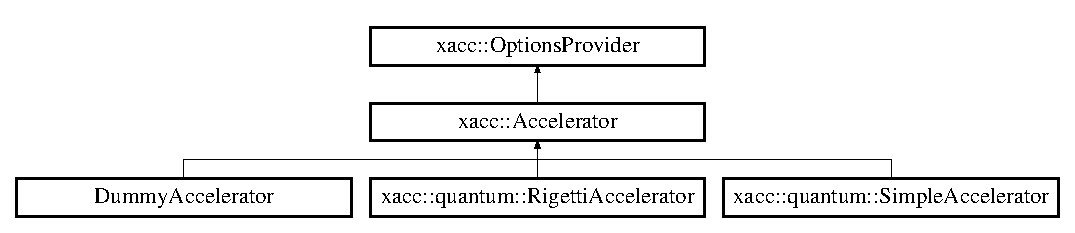
\includegraphics[height=2.679426cm]{a01435}
\end{center}
\end{figure}
\subsection*{Public Member Functions}
\begin{DoxyCompactItemize}
\item 
virtual Accelerator\+Type \hyperlink{a01435_aaffc3e4bb9880eb5041b1b58ee4c2665}{get\+Type} ()=0
\item 
virtual std\+::vector$<$ \hyperlink{a01503}{I\+R\+Transformation} $>$ \hyperlink{a01435_ad6e4a642dcb24e552675bcbeff1e1b04}{get\+I\+R\+Transformations} ()=0
\item 
virtual void \hyperlink{a01435_a89b3f3e6294f228abf03a410b0fb1674}{execute} (std\+::shared\+\_\+ptr$<$ \hyperlink{a01447}{Accelerator\+Buffer} $>$ buffer, const std\+::shared\+\_\+ptr$<$ \hyperlink{a01475}{Function} $>$ function)=0
\item 
virtual std\+::shared\+\_\+ptr$<$ \hyperlink{a01447}{Accelerator\+Buffer} $>$ \hyperlink{a01435_a064a2dbd58338364115c260267806945}{create\+Buffer} (const std\+::string \&var\+Id, const int size)=0
\item 
virtual std\+::shared\+\_\+ptr$<$ \hyperlink{a01447}{Accelerator\+Buffer} $>$ \hyperlink{a01435_ab3820be326e28a553fed1a824f4d41d0}{get\+Buffer} (const std\+::string \&varid)
\item 
virtual std\+::vector$<$ std\+::string $>$ \hyperlink{a01435_ae1463d7e405df89fa4af47e8922f4b82}{get\+Allocated\+Buffer\+Names} ()
\item 
virtual std\+::shared\+\_\+ptr$<$ options\+\_\+description $>$ \hyperlink{a01435_a98c9eda6b54367c75667ecfbbf167979}{get\+Options} ()
\item 
virtual \hyperlink{a01435_aed88ab0d71b765f0b0f512684ccd4b55}{$\sim$\+Accelerator} ()
\end{DoxyCompactItemize}
\subsection*{Protected Member Functions}
\begin{DoxyCompactItemize}
\item 
virtual bool \hyperlink{a01435_ae51584850faeec77299058383977ddeb}{is\+Valid\+Buffer\+Size} (const int N\+Bits)=0
\item 
void \hyperlink{a01435_ac3e781f42ec25e460174d4c41ea26b94}{store\+Buffer} (const std\+::string \&id, std\+::shared\+\_\+ptr$<$ \hyperlink{a01447}{Accelerator\+Buffer} $>$ b)
\end{DoxyCompactItemize}


\subsection{Detailed Description}
The \hyperlink{a01435}{Accelerator} class provides a high-\/level abstraction for X\+A\+CC\textquotesingle{}s interaction with attached post-\/exascale accelerators (quantum and neuromorphic processing units).

Derived Accelerators must provide a valid execute implementation that takes X\+A\+CC \hyperlink{a01499}{IR} and executes it on the attached hardware or simulator.

Derived Accelerators must provide a list of \hyperlink{a01503}{I\+R\+Transformation} instances that transform X\+A\+CC \hyperlink{a01499}{IR} to be amenable to execution on the hardware.

Derived Accelerators must provide implementations of create\+Buffer that provide a valid \hyperlink{a01447}{Accelerator\+Buffer} instance modeling the hardware memory or bits being computed on. Upon creating an \hyperlink{a01447}{Accelerator\+Buffer}, derived \hyperlink{a01435}{Accelerator} implementations must call the protected store\+Buffer method to store the \hyperlink{a01447}{Accelerator\+Buffer} for future reference by Compilers and clients of \hyperlink{a01435}{Accelerator}.

\begin{DoxyAuthor}{Author}
Alex Mc\+Caskey 
\end{DoxyAuthor}


\subsection{Constructor \& Destructor Documentation}
\mbox{\Hypertarget{a01435_aed88ab0d71b765f0b0f512684ccd4b55}\label{a01435_aed88ab0d71b765f0b0f512684ccd4b55}} 
\index{xacc\+::\+Accelerator@{xacc\+::\+Accelerator}!````~Accelerator@{$\sim$\+Accelerator}}
\index{````~Accelerator@{$\sim$\+Accelerator}!xacc\+::\+Accelerator@{xacc\+::\+Accelerator}}
\subsubsection{\texorpdfstring{$\sim$\+Accelerator()}{~Accelerator()}}
{\footnotesize\ttfamily virtual xacc\+::\+Accelerator\+::$\sim$\+Accelerator (\begin{DoxyParamCaption}{ }\end{DoxyParamCaption})\hspace{0.3cm}{\ttfamily [inline]}, {\ttfamily [virtual]}}

Destructor 

\subsection{Member Function Documentation}
\mbox{\Hypertarget{a01435_a064a2dbd58338364115c260267806945}\label{a01435_a064a2dbd58338364115c260267806945}} 
\index{xacc\+::\+Accelerator@{xacc\+::\+Accelerator}!create\+Buffer@{create\+Buffer}}
\index{create\+Buffer@{create\+Buffer}!xacc\+::\+Accelerator@{xacc\+::\+Accelerator}}
\subsubsection{\texorpdfstring{create\+Buffer()}{createBuffer()}}
{\footnotesize\ttfamily virtual std\+::shared\+\_\+ptr$<$\hyperlink{a01447}{Accelerator\+Buffer}$>$ xacc\+::\+Accelerator\+::create\+Buffer (\begin{DoxyParamCaption}\item[{const std\+::string \&}]{var\+Id,  }\item[{const int}]{size }\end{DoxyParamCaption})\hspace{0.3cm}{\ttfamily [pure virtual]}}

Create, store, and return an \hyperlink{a01447}{Accelerator\+Buffer} with the given variable id string and of the given number of bits. The string id serves as a unique identifier for future lookups and reuse of the \hyperlink{a01447}{Accelerator\+Buffer}.


\begin{DoxyParams}{Parameters}
{\em var\+Id} & The variable name of the created buffer \\
\hline
{\em size} & The number of bits in the created buffer \\
\hline
\end{DoxyParams}
\begin{DoxyReturn}{Returns}
buffer The buffer instance created. 
\end{DoxyReturn}


Implemented in \hyperlink{a01143_aa645e7ba6343aa9812836d1e141bd7c8}{Dummy\+Accelerator}, \hyperlink{a01083_a731551c94b1abef40d2cf032e8712df6}{xacc\+::quantum\+::\+Rigetti\+Accelerator}, and \hyperlink{a01111_adb9393692e9f484df241aa5d014030d1}{xacc\+::quantum\+::\+Simple\+Accelerator}.

\mbox{\Hypertarget{a01435_a89b3f3e6294f228abf03a410b0fb1674}\label{a01435_a89b3f3e6294f228abf03a410b0fb1674}} 
\index{xacc\+::\+Accelerator@{xacc\+::\+Accelerator}!execute@{execute}}
\index{execute@{execute}!xacc\+::\+Accelerator@{xacc\+::\+Accelerator}}
\subsubsection{\texorpdfstring{execute()}{execute()}}
{\footnotesize\ttfamily virtual void xacc\+::\+Accelerator\+::execute (\begin{DoxyParamCaption}\item[{std\+::shared\+\_\+ptr$<$ \hyperlink{a01447}{Accelerator\+Buffer} $>$}]{buffer,  }\item[{const std\+::shared\+\_\+ptr$<$ \hyperlink{a01475}{Function} $>$}]{function }\end{DoxyParamCaption})\hspace{0.3cm}{\ttfamily [pure virtual]}}

Execute the provided X\+A\+CC \hyperlink{a01499}{IR} \hyperlink{a01475}{Function} on the provided \hyperlink{a01447}{Accelerator\+Buffer}.


\begin{DoxyParams}{Parameters}
{\em buffer} & The buffer of bits this \hyperlink{a01435}{Accelerator} should operate on. \\
\hline
{\em function} & The kernel to execute. \\
\hline
\end{DoxyParams}


Implemented in \hyperlink{a01143_a389ba22af5d0d964f5d5367f01712b3c}{Dummy\+Accelerator}.

\mbox{\Hypertarget{a01435_ae1463d7e405df89fa4af47e8922f4b82}\label{a01435_ae1463d7e405df89fa4af47e8922f4b82}} 
\index{xacc\+::\+Accelerator@{xacc\+::\+Accelerator}!get\+Allocated\+Buffer\+Names@{get\+Allocated\+Buffer\+Names}}
\index{get\+Allocated\+Buffer\+Names@{get\+Allocated\+Buffer\+Names}!xacc\+::\+Accelerator@{xacc\+::\+Accelerator}}
\subsubsection{\texorpdfstring{get\+Allocated\+Buffer\+Names()}{getAllocatedBufferNames()}}
{\footnotesize\ttfamily virtual std\+::vector$<$std\+::string$>$ xacc\+::\+Accelerator\+::get\+Allocated\+Buffer\+Names (\begin{DoxyParamCaption}{ }\end{DoxyParamCaption})\hspace{0.3cm}{\ttfamily [inline]}, {\ttfamily [virtual]}}

Return all allocated \hyperlink{a01447}{Accelerator\+Buffer} variable names.

\begin{DoxyReturn}{Returns}
var\+Names The buffer variable names 
\end{DoxyReturn}
\mbox{\Hypertarget{a01435_ab3820be326e28a553fed1a824f4d41d0}\label{a01435_ab3820be326e28a553fed1a824f4d41d0}} 
\index{xacc\+::\+Accelerator@{xacc\+::\+Accelerator}!get\+Buffer@{get\+Buffer}}
\index{get\+Buffer@{get\+Buffer}!xacc\+::\+Accelerator@{xacc\+::\+Accelerator}}
\subsubsection{\texorpdfstring{get\+Buffer()}{getBuffer()}}
{\footnotesize\ttfamily virtual std\+::shared\+\_\+ptr$<$\hyperlink{a01447}{Accelerator\+Buffer}$>$ xacc\+::\+Accelerator\+::get\+Buffer (\begin{DoxyParamCaption}\item[{const std\+::string \&}]{varid }\end{DoxyParamCaption})\hspace{0.3cm}{\ttfamily [inline]}, {\ttfamily [virtual]}}

Return the stored \hyperlink{a01447}{Accelerator\+Buffer} with the provided string id.


\begin{DoxyParams}{Parameters}
{\em varid} & The variable name of the created buffer \\
\hline
\end{DoxyParams}
\begin{DoxyReturn}{Returns}
buffer The buffer with given varid. 
\end{DoxyReturn}
\mbox{\Hypertarget{a01435_ad6e4a642dcb24e552675bcbeff1e1b04}\label{a01435_ad6e4a642dcb24e552675bcbeff1e1b04}} 
\index{xacc\+::\+Accelerator@{xacc\+::\+Accelerator}!get\+I\+R\+Transformations@{get\+I\+R\+Transformations}}
\index{get\+I\+R\+Transformations@{get\+I\+R\+Transformations}!xacc\+::\+Accelerator@{xacc\+::\+Accelerator}}
\subsubsection{\texorpdfstring{get\+I\+R\+Transformations()}{getIRTransformations()}}
{\footnotesize\ttfamily virtual std\+::vector$<$\hyperlink{a01503}{I\+R\+Transformation}$>$ xacc\+::\+Accelerator\+::get\+I\+R\+Transformations (\begin{DoxyParamCaption}{ }\end{DoxyParamCaption})\hspace{0.3cm}{\ttfamily [pure virtual]}}

Return any \hyperlink{a01499}{IR} Transformations that must be applied to ensure the compiled \hyperlink{a01499}{IR} is amenable to execution on this \hyperlink{a01435}{Accelerator}.

\begin{DoxyReturn}{Returns}
transformations The \hyperlink{a01499}{IR} transformations this \hyperlink{a01435}{Accelerator} exposes 
\end{DoxyReturn}


Implemented in \hyperlink{a01083_a443683a1dfb000603c640b2ee303cf66}{xacc\+::quantum\+::\+Rigetti\+Accelerator}, \hyperlink{a01111_afc49c9e7973ba6c6ff9761c36198323d}{xacc\+::quantum\+::\+Simple\+Accelerator}, and \hyperlink{a01143_aac0e2ae753064701468fa1188ac7549f}{Dummy\+Accelerator}.

\mbox{\Hypertarget{a01435_a98c9eda6b54367c75667ecfbbf167979}\label{a01435_a98c9eda6b54367c75667ecfbbf167979}} 
\index{xacc\+::\+Accelerator@{xacc\+::\+Accelerator}!get\+Options@{get\+Options}}
\index{get\+Options@{get\+Options}!xacc\+::\+Accelerator@{xacc\+::\+Accelerator}}
\subsubsection{\texorpdfstring{get\+Options()}{getOptions()}}
{\footnotesize\ttfamily virtual std\+::shared\+\_\+ptr$<$options\+\_\+description$>$ xacc\+::\+Accelerator\+::get\+Options (\begin{DoxyParamCaption}{ }\end{DoxyParamCaption})\hspace{0.3cm}{\ttfamily [inline]}, {\ttfamily [virtual]}}

Return an empty options\+\_\+description, this is for subclasses to implement. 

Implements \hyperlink{a01543_a6d150954f852109bfe2c1ae90222926f}{xacc\+::\+Options\+Provider}.



Reimplemented in \hyperlink{a01083_a9ee9e62aecbccf193894ca3388676f9f}{xacc\+::quantum\+::\+Rigetti\+Accelerator}.

\mbox{\Hypertarget{a01435_aaffc3e4bb9880eb5041b1b58ee4c2665}\label{a01435_aaffc3e4bb9880eb5041b1b58ee4c2665}} 
\index{xacc\+::\+Accelerator@{xacc\+::\+Accelerator}!get\+Type@{get\+Type}}
\index{get\+Type@{get\+Type}!xacc\+::\+Accelerator@{xacc\+::\+Accelerator}}
\subsubsection{\texorpdfstring{get\+Type()}{getType()}}
{\footnotesize\ttfamily virtual Accelerator\+Type xacc\+::\+Accelerator\+::get\+Type (\begin{DoxyParamCaption}{ }\end{DoxyParamCaption})\hspace{0.3cm}{\ttfamily [pure virtual]}}

Return the type of this \hyperlink{a01435}{Accelerator}.

\begin{DoxyReturn}{Returns}
type The \hyperlink{a01435}{Accelerator} type -\/ Gate or A\+QC Q\+PU, or N\+PU 
\end{DoxyReturn}


Implemented in \hyperlink{a01143_acdfe3e856f2bacc9e0dc1a51782a52e3}{Dummy\+Accelerator}, \hyperlink{a01083_aab0d4674da5273d55407b9ab77cde890}{xacc\+::quantum\+::\+Rigetti\+Accelerator}, and \hyperlink{a01111_ad76eeb0bbd7de21aad5bd20d20970a98}{xacc\+::quantum\+::\+Simple\+Accelerator}.

\mbox{\Hypertarget{a01435_ae51584850faeec77299058383977ddeb}\label{a01435_ae51584850faeec77299058383977ddeb}} 
\index{xacc\+::\+Accelerator@{xacc\+::\+Accelerator}!is\+Valid\+Buffer\+Size@{is\+Valid\+Buffer\+Size}}
\index{is\+Valid\+Buffer\+Size@{is\+Valid\+Buffer\+Size}!xacc\+::\+Accelerator@{xacc\+::\+Accelerator}}
\subsubsection{\texorpdfstring{is\+Valid\+Buffer\+Size()}{isValidBufferSize()}}
{\footnotesize\ttfamily virtual bool xacc\+::\+Accelerator\+::is\+Valid\+Buffer\+Size (\begin{DoxyParamCaption}\item[{const int}]{N\+Bits }\end{DoxyParamCaption})\hspace{0.3cm}{\ttfamily [protected]}, {\ttfamily [pure virtual]}}

Return true if this \hyperlink{a01435}{Accelerator} can allocated N\+Bits number of bits. This is meant to be implemented and used by subclasses.


\begin{DoxyParams}{Parameters}
{\em N\+Bits} & The number of bits to allocate \\
\hline
\end{DoxyParams}
\begin{DoxyReturn}{Returns}
valid True if size is valid. 
\end{DoxyReturn}


Implemented in \hyperlink{a01143_a831ad0c71864920cc49a00d29768af8c}{Dummy\+Accelerator}, \hyperlink{a01083_a61352c07062597aad2393fbeed4cc025}{xacc\+::quantum\+::\+Rigetti\+Accelerator}, and \hyperlink{a01111_a60b9db2d6aed235857c45413a070338e}{xacc\+::quantum\+::\+Simple\+Accelerator}.

\mbox{\Hypertarget{a01435_ac3e781f42ec25e460174d4c41ea26b94}\label{a01435_ac3e781f42ec25e460174d4c41ea26b94}} 
\index{xacc\+::\+Accelerator@{xacc\+::\+Accelerator}!store\+Buffer@{store\+Buffer}}
\index{store\+Buffer@{store\+Buffer}!xacc\+::\+Accelerator@{xacc\+::\+Accelerator}}
\subsubsection{\texorpdfstring{store\+Buffer()}{storeBuffer()}}
{\footnotesize\ttfamily void xacc\+::\+Accelerator\+::store\+Buffer (\begin{DoxyParamCaption}\item[{const std\+::string \&}]{id,  }\item[{std\+::shared\+\_\+ptr$<$ \hyperlink{a01447}{Accelerator\+Buffer} $>$}]{b }\end{DoxyParamCaption})\hspace{0.3cm}{\ttfamily [inline]}, {\ttfamily [protected]}}

This protected method is to be used by derived Accelerators to store any created \hyperlink{a01447}{Accelerator\+Buffer}.


\begin{DoxyParams}{Parameters}
{\em id} & The variable name of the buffer to store \\
\hline
{\em b} & The buffer to store \\
\hline
\end{DoxyParams}


The documentation for this class was generated from the following file\+:\begin{DoxyCompactItemize}
\item 
Accelerator.\+hpp\end{DoxyCompactItemize}

\hypertarget{a01443}{}\section{xacc\+:\+:Accelerator\+Bit Class Reference}
\label{a01443}\index{xacc\+::\+Accelerator\+Bit@{xacc\+::\+Accelerator\+Bit}}


{\ttfamily \#include $<$Accelerator\+Buffer.\+hpp$>$}

\subsection*{Public Member Functions}
\begin{DoxyCompactItemize}
\item 
\hyperlink{a01443_a9a124c230c5cabeab53bac0820c0221a}{Accelerator\+Bit} ()
\item 
void \hyperlink{a01443_aa63a24980e831b9325a36836ab1c5495}{update} (int zero\+Or\+One)
\item 
Accelerator\+Bit\+State \hyperlink{a01443_a4a8dcc4fa02a5619f583961460c77057}{get\+State} ()
\end{DoxyCompactItemize}
\subsection*{Protected Attributes}
\begin{DoxyCompactItemize}
\item 
Accelerator\+Bit\+State \hyperlink{a01443_a4632123ac31aeed0dc97c65f8c792a85}{state}
\end{DoxyCompactItemize}


\subsection{Detailed Description}
The \hyperlink{a01443}{Accelerator\+Bit} wraps an Accelerator\+Bit\+Sate and provides a mechanism for updating that state.

\begin{DoxyAuthor}{Author}
Alex Mc\+Caskey 
\end{DoxyAuthor}


\subsection{Constructor \& Destructor Documentation}
\mbox{\Hypertarget{a01443_a9a124c230c5cabeab53bac0820c0221a}\label{a01443_a9a124c230c5cabeab53bac0820c0221a}} 
\index{xacc\+::\+Accelerator\+Bit@{xacc\+::\+Accelerator\+Bit}!Accelerator\+Bit@{Accelerator\+Bit}}
\index{Accelerator\+Bit@{Accelerator\+Bit}!xacc\+::\+Accelerator\+Bit@{xacc\+::\+Accelerator\+Bit}}
\subsubsection{\texorpdfstring{Accelerator\+Bit()}{AcceleratorBit()}}
{\footnotesize\ttfamily xacc\+::\+Accelerator\+Bit\+::\+Accelerator\+Bit (\begin{DoxyParamCaption}{ }\end{DoxyParamCaption})\hspace{0.3cm}{\ttfamily [inline]}}

The constructor, all bits are initialized to unknown state 

\subsection{Member Function Documentation}
\mbox{\Hypertarget{a01443_a4a8dcc4fa02a5619f583961460c77057}\label{a01443_a4a8dcc4fa02a5619f583961460c77057}} 
\index{xacc\+::\+Accelerator\+Bit@{xacc\+::\+Accelerator\+Bit}!get\+State@{get\+State}}
\index{get\+State@{get\+State}!xacc\+::\+Accelerator\+Bit@{xacc\+::\+Accelerator\+Bit}}
\subsubsection{\texorpdfstring{get\+State()}{getState()}}
{\footnotesize\ttfamily Accelerator\+Bit\+State xacc\+::\+Accelerator\+Bit\+::get\+State (\begin{DoxyParamCaption}{ }\end{DoxyParamCaption})\hspace{0.3cm}{\ttfamily [inline]}}

Return the value of this state \mbox{\Hypertarget{a01443_aa63a24980e831b9325a36836ab1c5495}\label{a01443_aa63a24980e831b9325a36836ab1c5495}} 
\index{xacc\+::\+Accelerator\+Bit@{xacc\+::\+Accelerator\+Bit}!update@{update}}
\index{update@{update}!xacc\+::\+Accelerator\+Bit@{xacc\+::\+Accelerator\+Bit}}
\subsubsection{\texorpdfstring{update()}{update()}}
{\footnotesize\ttfamily void xacc\+::\+Accelerator\+Bit\+::update (\begin{DoxyParamCaption}\item[{int}]{zero\+Or\+One }\end{DoxyParamCaption})\hspace{0.3cm}{\ttfamily [inline]}}

Update the Bit state to a one or zero 

\subsection{Member Data Documentation}
\mbox{\Hypertarget{a01443_a4632123ac31aeed0dc97c65f8c792a85}\label{a01443_a4632123ac31aeed0dc97c65f8c792a85}} 
\index{xacc\+::\+Accelerator\+Bit@{xacc\+::\+Accelerator\+Bit}!state@{state}}
\index{state@{state}!xacc\+::\+Accelerator\+Bit@{xacc\+::\+Accelerator\+Bit}}
\subsubsection{\texorpdfstring{state}{state}}
{\footnotesize\ttfamily Accelerator\+Bit\+State xacc\+::\+Accelerator\+Bit\+::state\hspace{0.3cm}{\ttfamily [protected]}}

The bit state 

The documentation for this class was generated from the following file\+:\begin{DoxyCompactItemize}
\item 
Accelerator\+Buffer.\+hpp\end{DoxyCompactItemize}

\hypertarget{a01447}{}\section{xacc\+:\+:Accelerator\+Buffer Class Reference}
\label{a01447}\index{xacc\+::\+Accelerator\+Buffer@{xacc\+::\+Accelerator\+Buffer}}


{\ttfamily \#include $<$Accelerator\+Buffer.\+hpp$>$}

Inheritance diagram for xacc\+:\+:Accelerator\+Buffer\+:\begin{figure}[H]
\begin{center}
\leavevmode
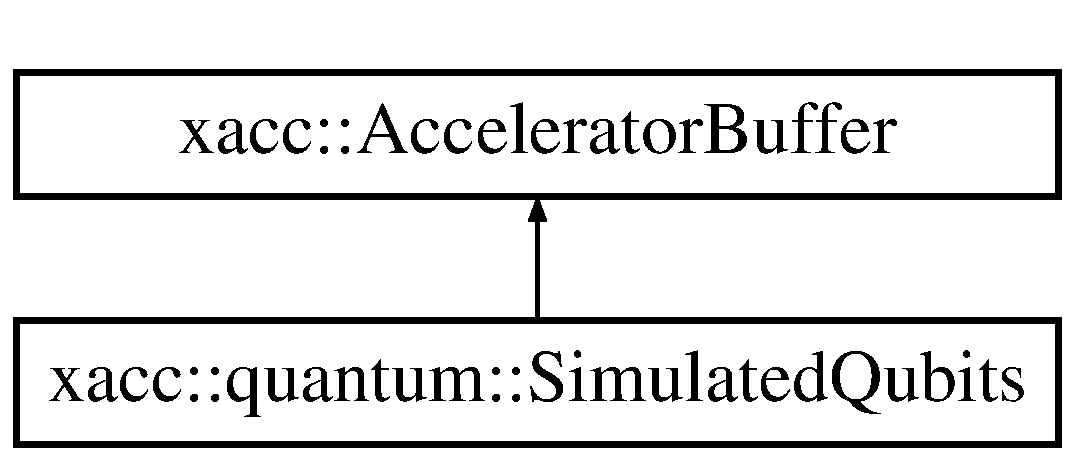
\includegraphics[height=2.000000cm]{a01447}
\end{center}
\end{figure}
\subsection*{Public Member Functions}
\begin{DoxyCompactItemize}
\item 
\hyperlink{a01447_ab606d8af942120d60b51a4fffcd75c98}{Accelerator\+Buffer} (const std\+::string \&str, const int N)
\item 
\mbox{\Hypertarget{a01447_ae6fc59d8a9abf1efce40427c7ba12c57}\label{a01447_ae6fc59d8a9abf1efce40427c7ba12c57}} 
{\footnotesize template$<$typename ... Indices$>$ }\\{\bfseries Accelerator\+Buffer} (const std\+::string \&str, int first\+Index, Indices ... indices)
\item 
\mbox{\Hypertarget{a01447_aa2a3101c2e3ae3550172bf49f9587f3b}\label{a01447_aa2a3101c2e3ae3550172bf49f9587f3b}} 
int {\bfseries size} ()
\item 
\mbox{\Hypertarget{a01447_ad5b646e9efc21b6d0bcc22cd6f649c22}\label{a01447_ad5b646e9efc21b6d0bcc22cd6f649c22}} 
std\+::string {\bfseries name} ()
\item 
\mbox{\Hypertarget{a01447_aa6d6e9cfee6170333c1f03507345743f}\label{a01447_aa6d6e9cfee6170333c1f03507345743f}} 
void {\bfseries reset\+Buffer} ()
\item 
\mbox{\Hypertarget{a01447_a4bc0edbe9aa0d463f67ddcc38265066f}\label{a01447_a4bc0edbe9aa0d463f67ddcc38265066f}} 
void {\bfseries update\+Bit} (const int idx, int zero\+Or\+One)
\item 
\mbox{\Hypertarget{a01447_ac161c4f984f774d08197871094aabc67}\label{a01447_ac161c4f984f774d08197871094aabc67}} 
void {\bfseries append\+Measurement} (const boost\+::dynamic\+\_\+bitset$<$$>$ \&measurement)
\item 
\mbox{\Hypertarget{a01447_aaddd3a5968067dd230f48dacc8d6a747}\label{a01447_aaddd3a5968067dd230f48dacc8d6a747}} 
double {\bfseries get\+Average} () const
\item 
\mbox{\Hypertarget{a01447_aba6ef359f3117faa98f0eb8da90d909e}\label{a01447_aba6ef359f3117faa98f0eb8da90d909e}} 
Accelerator\+Bit\+State {\bfseries get\+Accelerator\+Bit\+State} (const int idx)
\item 
\mbox{\Hypertarget{a01447_add0835e188f0eda4f1b68a28ddc79786}\label{a01447_add0835e188f0eda4f1b68a28ddc79786}} 
virtual void {\bfseries print} ()
\item 
\mbox{\Hypertarget{a01447_a7c59462451223772b41ef232b06a7dfa}\label{a01447_a7c59462451223772b41ef232b06a7dfa}} 
virtual void {\bfseries print} (std\+::ostream \&stream)
\end{DoxyCompactItemize}
\subsection*{Protected Attributes}
\begin{DoxyCompactItemize}
\item 
\mbox{\Hypertarget{a01447_a5464b23a964985df2547f657877c9ea5}\label{a01447_a5464b23a964985df2547f657877c9ea5}} 
std\+::vector$<$ boost\+::dynamic\+\_\+bitset$<$$>$ $>$ {\bfseries measurements}
\item 
\mbox{\Hypertarget{a01447_a3198e034d07d9b77b62da03e6592a221}\label{a01447_a3198e034d07d9b77b62da03e6592a221}} 
std\+::string {\bfseries buffer\+Id}
\item 
\mbox{\Hypertarget{a01447_ab6dbb8c22f8adc6aba34b00a84066854}\label{a01447_ab6dbb8c22f8adc6aba34b00a84066854}} 
std\+::vector$<$ \hyperlink{a01443}{Accelerator\+Bit} $>$ {\bfseries bits}
\end{DoxyCompactItemize}


\subsection{Detailed Description}
The \hyperlink{a01447}{Accelerator\+Buffer} models an allocated buffer of bits that are operated on by a kernel. As such, the \hyperlink{a01447}{Accelerator\+Buffer}\textquotesingle{}s primary role is to store \hyperlink{a01435}{Accelerator} execution results.

\begin{DoxyAuthor}{Author}
Alex Mc\+Caskey 
\end{DoxyAuthor}


\subsection{Constructor \& Destructor Documentation}
\mbox{\Hypertarget{a01447_ab606d8af942120d60b51a4fffcd75c98}\label{a01447_ab606d8af942120d60b51a4fffcd75c98}} 
\index{xacc\+::\+Accelerator\+Buffer@{xacc\+::\+Accelerator\+Buffer}!Accelerator\+Buffer@{Accelerator\+Buffer}}
\index{Accelerator\+Buffer@{Accelerator\+Buffer}!xacc\+::\+Accelerator\+Buffer@{xacc\+::\+Accelerator\+Buffer}}
\subsubsection{\texorpdfstring{Accelerator\+Buffer()}{AcceleratorBuffer()}}
{\footnotesize\ttfamily xacc\+::\+Accelerator\+Buffer\+::\+Accelerator\+Buffer (\begin{DoxyParamCaption}\item[{const std\+::string \&}]{str,  }\item[{const int}]{N }\end{DoxyParamCaption})\hspace{0.3cm}{\ttfamily [inline]}}

The Constructor 

The documentation for this class was generated from the following file\+:\begin{DoxyCompactItemize}
\item 
Accelerator\+Buffer.\+hpp\end{DoxyCompactItemize}

\hypertarget{a01467}{}\section{xacc\+:\+:Algorithm\+Generator Class Reference}
\label{a01467}\index{xacc\+::\+Algorithm\+Generator@{xacc\+::\+Algorithm\+Generator}}


{\ttfamily \#include $<$Algorithm\+Generator.\+hpp$>$}

Inheritance diagram for xacc\+:\+:Algorithm\+Generator\+:\begin{figure}[H]
\begin{center}
\leavevmode
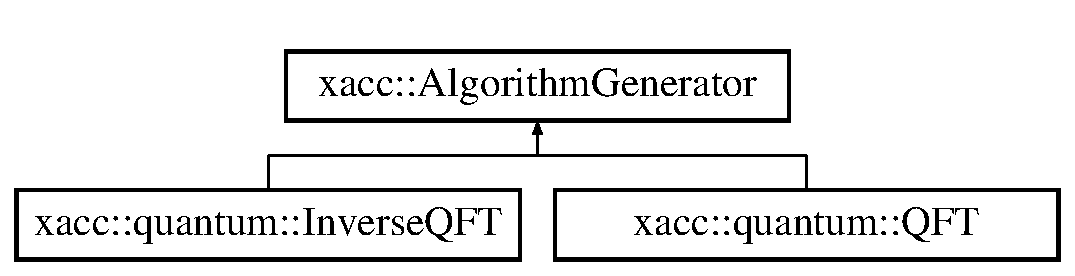
\includegraphics[height=2.000000cm]{a01467}
\end{center}
\end{figure}
\subsection*{Public Member Functions}
\begin{DoxyCompactItemize}
\item 
virtual std\+::shared\+\_\+ptr$<$ \hyperlink{a01475}{Function} $>$ \hyperlink{a01467_a73023c06f0f0c62ad56ab4187b18b096}{generate\+Algorithm} (std\+::vector$<$ int $>$ bits)=0
\item 
virtual \hyperlink{a01467_a096f66aa8d65f5aa3276915768159579}{$\sim$\+Algorithm\+Generator} ()
\end{DoxyCompactItemize}


\subsection{Detailed Description}
The \hyperlink{a01467}{Algorithm\+Generator} interface provides a mechanism for generating algorithms modeled as an X\+A\+CC \hyperlink{a01475}{Function} instance.

\begin{DoxyAuthor}{Author}
Alex Mc\+Caskey 
\end{DoxyAuthor}


\subsection{Constructor \& Destructor Documentation}
\mbox{\Hypertarget{a01467_a096f66aa8d65f5aa3276915768159579}\label{a01467_a096f66aa8d65f5aa3276915768159579}} 
\index{xacc\+::\+Algorithm\+Generator@{xacc\+::\+Algorithm\+Generator}!````~Algorithm\+Generator@{$\sim$\+Algorithm\+Generator}}
\index{````~Algorithm\+Generator@{$\sim$\+Algorithm\+Generator}!xacc\+::\+Algorithm\+Generator@{xacc\+::\+Algorithm\+Generator}}
\subsubsection{\texorpdfstring{$\sim$\+Algorithm\+Generator()}{~AlgorithmGenerator()}}
{\footnotesize\ttfamily virtual xacc\+::\+Algorithm\+Generator\+::$\sim$\+Algorithm\+Generator (\begin{DoxyParamCaption}{ }\end{DoxyParamCaption})\hspace{0.3cm}{\ttfamily [inline]}, {\ttfamily [virtual]}}

The destructor 

\subsection{Member Function Documentation}
\mbox{\Hypertarget{a01467_a73023c06f0f0c62ad56ab4187b18b096}\label{a01467_a73023c06f0f0c62ad56ab4187b18b096}} 
\index{xacc\+::\+Algorithm\+Generator@{xacc\+::\+Algorithm\+Generator}!generate\+Algorithm@{generate\+Algorithm}}
\index{generate\+Algorithm@{generate\+Algorithm}!xacc\+::\+Algorithm\+Generator@{xacc\+::\+Algorithm\+Generator}}
\subsubsection{\texorpdfstring{generate\+Algorithm()}{generateAlgorithm()}}
{\footnotesize\ttfamily virtual std\+::shared\+\_\+ptr$<$\hyperlink{a01475}{Function}$>$ xacc\+::\+Algorithm\+Generator\+::generate\+Algorithm (\begin{DoxyParamCaption}\item[{std\+::vector$<$ int $>$}]{bits }\end{DoxyParamCaption})\hspace{0.3cm}{\ttfamily [pure virtual]}}

Implementations of this method generate a \hyperlink{a01475}{Function} \hyperlink{a01499}{IR} instance corresponding to the implementation\textquotesingle{}s modeled algorithm. The algorithm is specified to operate over the provided bits.


\begin{DoxyParams}{Parameters}
{\em bits} & The bits this algorithm operates on \\
\hline
\end{DoxyParams}
\begin{DoxyReturn}{Returns}
function The algorithm represented as an \hyperlink{a01499}{IR} \hyperlink{a01475}{Function} 
\end{DoxyReturn}


Implemented in \hyperlink{a01151_ac093c288bc9fc069464fc3fd2cc0ac21}{xacc\+::quantum\+::\+Q\+FT}, and \hyperlink{a01147_af42e466bf02dbd60670d20aa55cfb08d}{xacc\+::quantum\+::\+Inverse\+Q\+FT}.



The documentation for this class was generated from the following file\+:\begin{DoxyCompactItemize}
\item 
Algorithm\+Generator.\+hpp\end{DoxyCompactItemize}

\hypertarget{a01227}{}\section{xacc\+:\+:Runtime\+Options Class Reference}
\label{a01227}\index{xacc\+::\+Runtime\+Options@{xacc\+::\+Runtime\+Options}}


{\ttfamily \#include $<$Runtime\+Options.\+hpp$>$}

Inheritance diagram for xacc\+:\+:Runtime\+Options\+:\begin{figure}[H]
\begin{center}
\leavevmode
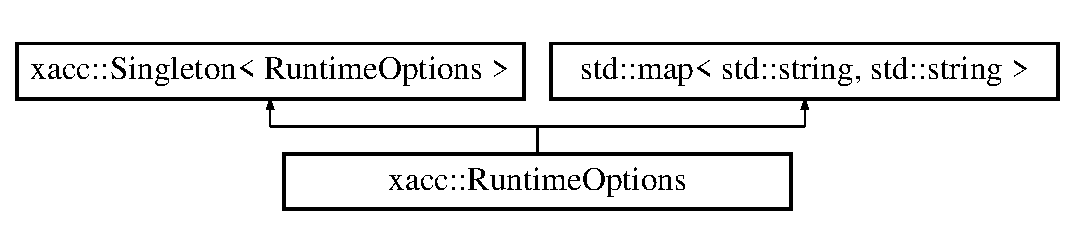
\includegraphics[height=2.000000cm]{a01227}
\end{center}
\end{figure}
\subsection*{Public Member Functions}
\begin{DoxyCompactItemize}
\item 
bool \hyperlink{a01227_a3603aecb87461efedd0fabbef966c80c}{exists} (const std\+::string \&key)
\end{DoxyCompactItemize}
\subsection*{Additional Inherited Members}


\subsection{Detailed Description}
The \hyperlink{a01227}{Runtime\+Options} class is a \hyperlink{a01231}{Singleton} mapping of string keys to string values. It is used throughout X\+A\+CC to provide and share runtime options that are provided from X\+A\+CC users via the command line. 

\subsection{Member Function Documentation}
\mbox{\Hypertarget{a01227_a3603aecb87461efedd0fabbef966c80c}\label{a01227_a3603aecb87461efedd0fabbef966c80c}} 
\index{xacc\+::\+Runtime\+Options@{xacc\+::\+Runtime\+Options}!exists@{exists}}
\index{exists@{exists}!xacc\+::\+Runtime\+Options@{xacc\+::\+Runtime\+Options}}
\subsubsection{\texorpdfstring{exists()}{exists()}}
{\footnotesize\ttfamily bool xacc\+::\+Runtime\+Options\+::exists (\begin{DoxyParamCaption}\item[{const std\+::string \&}]{key }\end{DoxyParamCaption})\hspace{0.3cm}{\ttfamily [inline]}}

Convenience method to get whether the give key exists in the \hyperlink{a01227}{Runtime\+Options}.


\begin{DoxyParams}{Parameters}
{\em key} & The key to check exists \\
\hline
\end{DoxyParams}


The documentation for this class was generated from the following file\+:\begin{DoxyCompactItemize}
\item 
Runtime\+Options.\+hpp\end{DoxyCompactItemize}

\hypertarget{a01363}{}\section{fire\+:\+:array\+\_\+size$<$ T $>$ Struct Template Reference}
\label{a01363}\index{fire\+::array\+\_\+size$<$ T $>$@{fire\+::array\+\_\+size$<$ T $>$}}


{\ttfamily \#include $<$Tensor\+Utils.\+hpp$>$}



\subsection{Detailed Description}
\subsubsection*{template$<$typename T$>$\newline
struct fire\+::array\+\_\+size$<$ T $>$}

This utility template enables the use of std\+::array size integer. 

The documentation for this struct was generated from the following file\+:\begin{DoxyCompactItemize}
\item 
Tensor\+Utils.\+hpp\end{DoxyCompactItemize}

\hypertarget{a01367}{}\section{fire\+:\+:array\+\_\+size$<$ std\+:\+:array$<$ T, N $>$ $>$ Struct Template Reference}
\label{a01367}\index{fire\+::array\+\_\+size$<$ std\+::array$<$ T, N $>$ $>$@{fire\+::array\+\_\+size$<$ std\+::array$<$ T, N $>$ $>$}}
\subsection*{Static Public Attributes}
\begin{DoxyCompactItemize}
\item 
\mbox{\Hypertarget{a01367_ab92887f3c176f5d68d76c67b4db2f112}\label{a01367_ab92887f3c176f5d68d76c67b4db2f112}} 
static const size\+\_\+t {\bfseries value} = N
\end{DoxyCompactItemize}


The documentation for this struct was generated from the following file\+:\begin{DoxyCompactItemize}
\item 
Tensor\+Utils.\+hpp\end{DoxyCompactItemize}

\hypertarget{a01559}{}\section{Bad\+Vertex Class Reference}
\label{a01559}\index{Bad\+Vertex@{Bad\+Vertex}}


The documentation for this class was generated from the following file\+:\begin{DoxyCompactItemize}
\item 
Graph\+Tester.\+cpp\end{DoxyCompactItemize}

\hypertarget{a01495}{}\section{xacc\+:\+:Base\+Instruction\+Visitable Class Reference}
\label{a01495}\index{xacc\+::\+Base\+Instruction\+Visitable@{xacc\+::\+Base\+Instruction\+Visitable}}


{\ttfamily \#include $<$Instruction\+Visitor.\+hpp$>$}

Inheritance diagram for xacc\+:\+:Base\+Instruction\+Visitable\+:\begin{figure}[H]
\begin{center}
\leavevmode
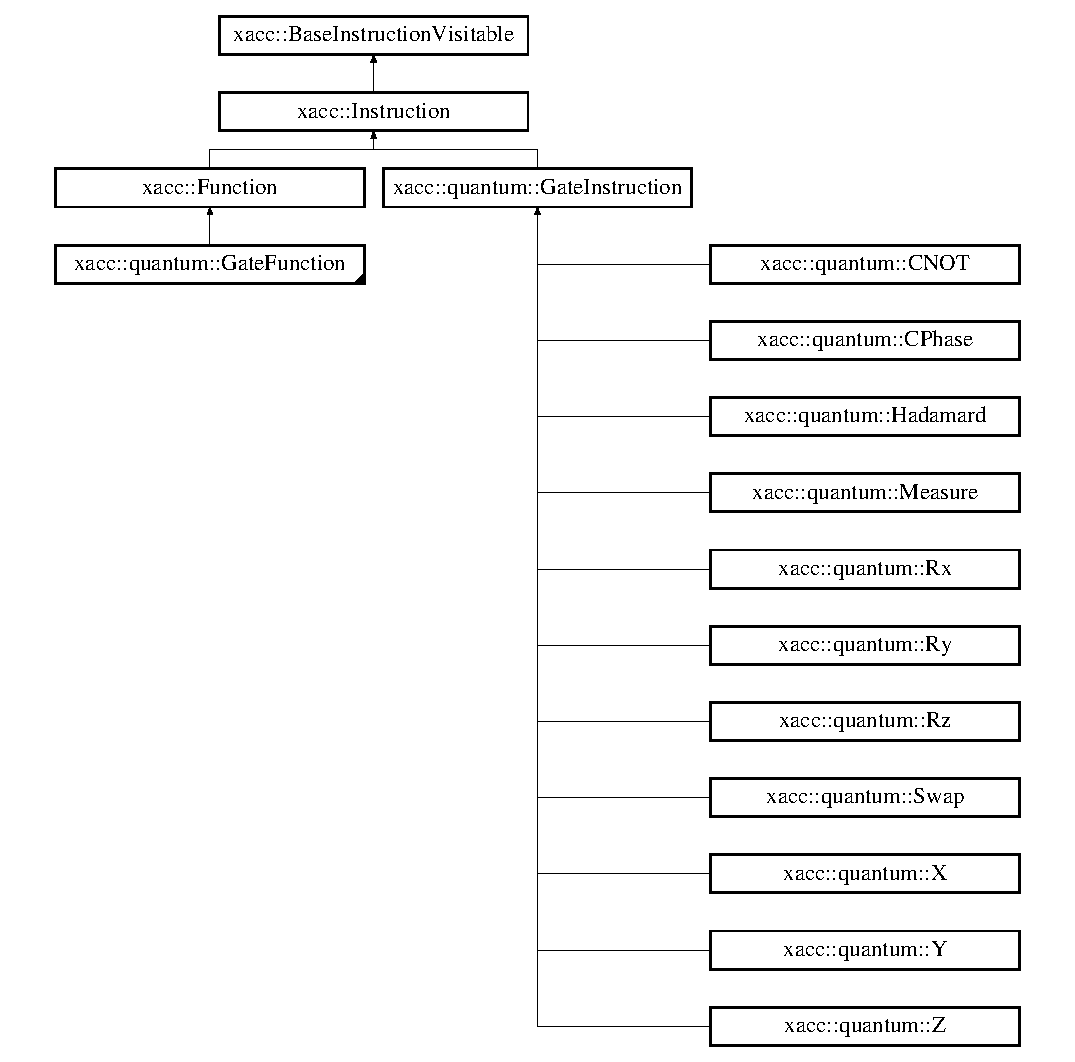
\includegraphics[height=12.000000cm]{a01495}
\end{center}
\end{figure}
\subsection*{Public Member Functions}
\begin{DoxyCompactItemize}
\item 
virtual void \hyperlink{a01495_a4ae295a7f83d57c6f1f912adc90274ea}{accept} (std\+::shared\+\_\+ptr$<$ \hyperlink{a01487}{Base\+Instruction\+Visitor} $>$ visitor)=0
\item 
virtual void \hyperlink{a01495_ad6b9ad95c14580cc86ca87cd464262c3}{accept} (\hyperlink{a01487}{Base\+Instruction\+Visitor} $\ast$visitor)=0
\item 
virtual \hyperlink{a01495_a3a291d247b18ea7620dd8d97dfb595f4}{$\sim$\+Base\+Instruction\+Visitable} ()
\end{DoxyCompactItemize}
\subsection*{Static Protected Member Functions}
\begin{DoxyCompactItemize}
\item 
{\footnotesize template$<$class T $>$ }\\static void \hyperlink{a01495_a2f18b9fcb48f42d190a9f5180b7b59c5}{accept\+Impl} (T \&visited, std\+::shared\+\_\+ptr$<$ \hyperlink{a01487}{Base\+Instruction\+Visitor} $>$ visitor)
\item 
{\footnotesize template$<$class T $>$ }\\static void \hyperlink{a01495_a80c7bb995faa54644f822fa48176c6cb}{accept\+Impl} (T \&visited, \hyperlink{a01487}{Base\+Instruction\+Visitor} $\ast$visitor)
\end{DoxyCompactItemize}


\subsection{Detailed Description}
\hyperlink{a01495}{Base\+Instruction\+Visitable} is an interface that is to be implemented by any and all Instructions that want to be available for visitation. Derivations of this class simply inherit from \hyperlink{a01495}{Base\+Instruction\+Visitable} and declare the D\+E\+F\+I\+N\+E\+\_\+\+V\+I\+S\+I\+T\+A\+B\+LE macro alongside the rest of the classes member methods. 

\subsection{Constructor \& Destructor Documentation}
\mbox{\Hypertarget{a01495_a3a291d247b18ea7620dd8d97dfb595f4}\label{a01495_a3a291d247b18ea7620dd8d97dfb595f4}} 
\index{xacc\+::\+Base\+Instruction\+Visitable@{xacc\+::\+Base\+Instruction\+Visitable}!````~Base\+Instruction\+Visitable@{$\sim$\+Base\+Instruction\+Visitable}}
\index{````~Base\+Instruction\+Visitable@{$\sim$\+Base\+Instruction\+Visitable}!xacc\+::\+Base\+Instruction\+Visitable@{xacc\+::\+Base\+Instruction\+Visitable}}
\subsubsection{\texorpdfstring{$\sim$\+Base\+Instruction\+Visitable()}{~BaseInstructionVisitable()}}
{\footnotesize\ttfamily virtual xacc\+::\+Base\+Instruction\+Visitable\+::$\sim$\+Base\+Instruction\+Visitable (\begin{DoxyParamCaption}{ }\end{DoxyParamCaption})\hspace{0.3cm}{\ttfamily [inline]}, {\ttfamily [virtual]}}

The Destructor 

\subsection{Member Function Documentation}
\mbox{\Hypertarget{a01495_a4ae295a7f83d57c6f1f912adc90274ea}\label{a01495_a4ae295a7f83d57c6f1f912adc90274ea}} 
\index{xacc\+::\+Base\+Instruction\+Visitable@{xacc\+::\+Base\+Instruction\+Visitable}!accept@{accept}}
\index{accept@{accept}!xacc\+::\+Base\+Instruction\+Visitable@{xacc\+::\+Base\+Instruction\+Visitable}}
\subsubsection{\texorpdfstring{accept()}{accept()}\hspace{0.1cm}{\footnotesize\ttfamily [1/2]}}
{\footnotesize\ttfamily virtual void xacc\+::\+Base\+Instruction\+Visitable\+::accept (\begin{DoxyParamCaption}\item[{std\+::shared\+\_\+ptr$<$ \hyperlink{a01487}{Base\+Instruction\+Visitor} $>$}]{visitor }\end{DoxyParamCaption})\hspace{0.3cm}{\ttfamily [pure virtual]}}

Accept the provided \hyperlink{a01487}{Base\+Instruction\+Visitor} as a shared pointer. 
\begin{DoxyParams}{Parameters}
{\em visitor} & The visitor to invoke visit() on. \\
\hline
\end{DoxyParams}
\mbox{\Hypertarget{a01495_ad6b9ad95c14580cc86ca87cd464262c3}\label{a01495_ad6b9ad95c14580cc86ca87cd464262c3}} 
\index{xacc\+::\+Base\+Instruction\+Visitable@{xacc\+::\+Base\+Instruction\+Visitable}!accept@{accept}}
\index{accept@{accept}!xacc\+::\+Base\+Instruction\+Visitable@{xacc\+::\+Base\+Instruction\+Visitable}}
\subsubsection{\texorpdfstring{accept()}{accept()}\hspace{0.1cm}{\footnotesize\ttfamily [2/2]}}
{\footnotesize\ttfamily virtual void xacc\+::\+Base\+Instruction\+Visitable\+::accept (\begin{DoxyParamCaption}\item[{\hyperlink{a01487}{Base\+Instruction\+Visitor} $\ast$}]{visitor }\end{DoxyParamCaption})\hspace{0.3cm}{\ttfamily [pure virtual]}}

Accept the provided \hyperlink{a01487}{Base\+Instruction\+Visitor} as a raw pointer. 
\begin{DoxyParams}{Parameters}
{\em visitor} & The visitor to invoke visit() on. \\
\hline
\end{DoxyParams}
\mbox{\Hypertarget{a01495_a2f18b9fcb48f42d190a9f5180b7b59c5}\label{a01495_a2f18b9fcb48f42d190a9f5180b7b59c5}} 
\index{xacc\+::\+Base\+Instruction\+Visitable@{xacc\+::\+Base\+Instruction\+Visitable}!accept\+Impl@{accept\+Impl}}
\index{accept\+Impl@{accept\+Impl}!xacc\+::\+Base\+Instruction\+Visitable@{xacc\+::\+Base\+Instruction\+Visitable}}
\subsubsection{\texorpdfstring{accept\+Impl()}{acceptImpl()}\hspace{0.1cm}{\footnotesize\ttfamily [1/2]}}
{\footnotesize\ttfamily template$<$class T $>$ \\
static void xacc\+::\+Base\+Instruction\+Visitable\+::accept\+Impl (\begin{DoxyParamCaption}\item[{T \&}]{visited,  }\item[{std\+::shared\+\_\+ptr$<$ \hyperlink{a01487}{Base\+Instruction\+Visitor} $>$}]{visitor }\end{DoxyParamCaption})\hspace{0.3cm}{\ttfamily [inline]}, {\ttfamily [static]}, {\ttfamily [protected]}}

This method is invoked by the D\+E\+F\+I\+N\+E\+\_\+\+V\+I\+S\+I\+T\+A\+B\+LE macro to invoke the visit method on the provided visitor. This method takes the visitor as a shared pointer. \mbox{\Hypertarget{a01495_a80c7bb995faa54644f822fa48176c6cb}\label{a01495_a80c7bb995faa54644f822fa48176c6cb}} 
\index{xacc\+::\+Base\+Instruction\+Visitable@{xacc\+::\+Base\+Instruction\+Visitable}!accept\+Impl@{accept\+Impl}}
\index{accept\+Impl@{accept\+Impl}!xacc\+::\+Base\+Instruction\+Visitable@{xacc\+::\+Base\+Instruction\+Visitable}}
\subsubsection{\texorpdfstring{accept\+Impl()}{acceptImpl()}\hspace{0.1cm}{\footnotesize\ttfamily [2/2]}}
{\footnotesize\ttfamily template$<$class T $>$ \\
static void xacc\+::\+Base\+Instruction\+Visitable\+::accept\+Impl (\begin{DoxyParamCaption}\item[{T \&}]{visited,  }\item[{\hyperlink{a01487}{Base\+Instruction\+Visitor} $\ast$}]{visitor }\end{DoxyParamCaption})\hspace{0.3cm}{\ttfamily [inline]}, {\ttfamily [static]}, {\ttfamily [protected]}}

This method is invoked by the D\+E\+F\+I\+N\+E\+\_\+\+V\+I\+S\+I\+T\+A\+B\+LE macro to invoke the visit method on the provided visitor. This method takes the visitor as a raw pointer. 

The documentation for this class was generated from the following file\+:\begin{DoxyCompactItemize}
\item 
Instruction\+Visitor.\+hpp\end{DoxyCompactItemize}

\hypertarget{a01487}{}\section{xacc\+:\+:Base\+Instruction\+Visitor Class Reference}
\label{a01487}\index{xacc\+::\+Base\+Instruction\+Visitor@{xacc\+::\+Base\+Instruction\+Visitor}}


{\ttfamily \#include $<$Instruction\+Visitor.\+hpp$>$}

Inheritance diagram for xacc\+:\+:Base\+Instruction\+Visitor\+:\begin{figure}[H]
\begin{center}
\leavevmode
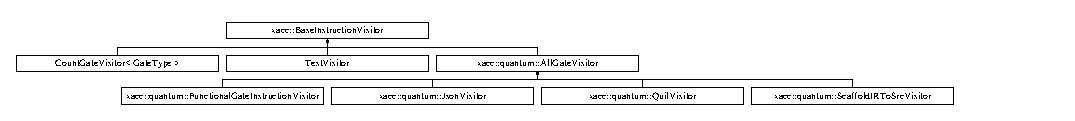
\includegraphics[height=1.183099cm]{a01487}
\end{center}
\end{figure}
\subsection*{Public Member Functions}
\begin{DoxyCompactItemize}
\item 
virtual \hyperlink{a01487_aa6f5104f5868fe1eca9be4dc4036eba4}{$\sim$\+Base\+Instruction\+Visitor} ()
\end{DoxyCompactItemize}


\subsection{Detailed Description}
The \hyperlink{a01487}{Base\+Instruction\+Visitor} is a base class for all classes that are \hyperlink{a01479}{Instruction} visitors. It basically provides a means for passing instruction visitor handles in a polymorphic manner. 

\subsection{Constructor \& Destructor Documentation}
\mbox{\Hypertarget{a01487_aa6f5104f5868fe1eca9be4dc4036eba4}\label{a01487_aa6f5104f5868fe1eca9be4dc4036eba4}} 
\index{xacc\+::\+Base\+Instruction\+Visitor@{xacc\+::\+Base\+Instruction\+Visitor}!````~Base\+Instruction\+Visitor@{$\sim$\+Base\+Instruction\+Visitor}}
\index{````~Base\+Instruction\+Visitor@{$\sim$\+Base\+Instruction\+Visitor}!xacc\+::\+Base\+Instruction\+Visitor@{xacc\+::\+Base\+Instruction\+Visitor}}
\subsubsection{\texorpdfstring{$\sim$\+Base\+Instruction\+Visitor()}{~BaseInstructionVisitor()}}
{\footnotesize\ttfamily virtual xacc\+::\+Base\+Instruction\+Visitor\+::$\sim$\+Base\+Instruction\+Visitor (\begin{DoxyParamCaption}{ }\end{DoxyParamCaption})\hspace{0.3cm}{\ttfamily [inline]}, {\ttfamily [virtual]}}

The destructor 

The documentation for this class was generated from the following file\+:\begin{DoxyCompactItemize}
\item 
Instruction\+Visitor.\+hpp\end{DoxyCompactItemize}

\hypertarget{a01323}{}\section{Block\+Generator Struct Reference}
\label{a01323}\index{Block\+Generator@{Block\+Generator}}


The documentation for this struct was generated from the following file\+:\begin{DoxyCompactItemize}
\item 
I\+N\+I\+Property\+Parser\+Test.\+cpp\end{DoxyCompactItemize}

\hypertarget{a01167}{}\section{xacc\+:\+:quantum\+:\+:Circuit\+Node Class Reference}
\label{a01167}\index{xacc\+::quantum\+::\+Circuit\+Node@{xacc\+::quantum\+::\+Circuit\+Node}}


{\ttfamily \#include $<$Gate\+Q\+I\+R.\+hpp$>$}

Inheritance diagram for xacc\+:\+:quantum\+:\+:Circuit\+Node\+:\begin{figure}[H]
\begin{center}
\leavevmode
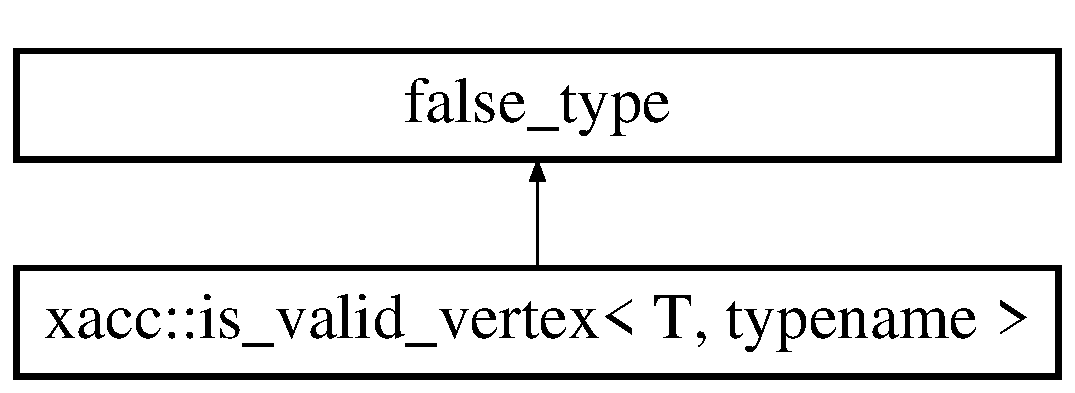
\includegraphics[height=1.060606cm]{a01167}
\end{center}
\end{figure}
\subsection*{Additional Inherited Members}


\subsection{Detailed Description}
\hyperlink{a01167}{Circuit\+Node} subclasses Q\+C\+I\+Vertex to provide the following parameters in the given order\+:

Parameters\+: Gate, Layer (ie time sequence), Gate Vertex Id, Qubit Ids that the gate acts on, enabled state, vector of parameters names 

The documentation for this class was generated from the following files\+:\begin{DoxyCompactItemize}
\item 
Gate\+Q\+I\+R.\+hpp\item 
Quantum\+Circuit.\+hpp\end{DoxyCompactItemize}

apt-\/get -\/y upgrade \&\& apt-\/get -\/y update \&\& apt-\/get install -\/y software-\/properties-\/common \&\& add-\/apt-\/repository ppa\+:ubuntu-\/toolchain-\/r/test \section*{install xacc deps}

apt-\/get -\/y update \&\& apt-\/get install -\/y \$(dpkg --info xacc\+\_\+1.\+0\+\_\+amd64.\+deb $\vert$ grep Depends $\vert$ sed \char`\"{}s/.$\ast$ends\+:\textbackslash{} //\char`\"{} $\vert$ sed \textquotesingle{}s/,//g\textquotesingle{}) git cmake libspdlog-\/dev 
\hypertarget{a01175}{}\section{xacc\+:\+:IR Class Reference}
\label{a01175}\index{xacc\+::\+IR@{xacc\+::\+IR}}


{\ttfamily \#include $<$I\+R.\+hpp$>$}

Inheritance diagram for xacc\+:\+:IR\+:\begin{figure}[H]
\begin{center}
\leavevmode
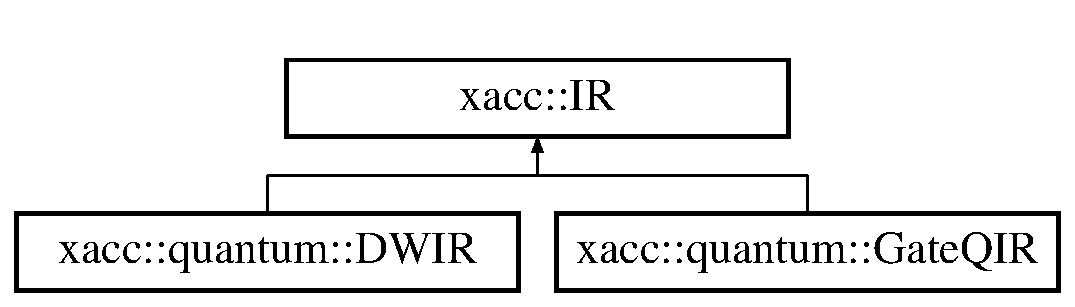
\includegraphics[height=2.000000cm]{a01175}
\end{center}
\end{figure}
\subsection*{Public Member Functions}
\begin{DoxyCompactItemize}
\item 
virtual std\+::string \hyperlink{a01175_a8356cdff1919b88eabeb84fd7450cdb6}{to\+Assembly\+String} (const std\+::string \&kernel\+Name, const std\+::string \&acc\+Buffer\+Var\+Name)=0
\item 
virtual void \hyperlink{a01175_a414b72224d88473ad6190bb88102a3ea}{persist} (std\+::ostream \&out\+Stream)=0
\item 
virtual void \hyperlink{a01175_a444c2e4dc0faac500fb70fa93997e9bc}{load} (std\+::istream \&in\+Stream)=0
\item 
virtual void \hyperlink{a01175_abbbf8e6993c518597de32cd05d49d737}{add\+Kernel} (std\+::shared\+\_\+ptr$<$ \hyperlink{a01151}{Function} $>$ kernel)=0
\item 
virtual bool \hyperlink{a01175_afc9ccf5126f3fed19c2e879133b2f6d8}{kernel\+Exists} (const std\+::string \&name)=0
\item 
virtual std\+::shared\+\_\+ptr$<$ \hyperlink{a01151}{Function} $>$ \hyperlink{a01175_a6f49b4ba4b3a15142b04873284885f0d}{get\+Kernel} (const std\+::string \&name)=0
\item 
virtual std\+::vector$<$ std\+::shared\+\_\+ptr$<$ \hyperlink{a01151}{Function} $>$ $>$ \hyperlink{a01175_a88c50bfc5b279145360ddc0c3a703b9b}{get\+Kernels} ()=0
\item 
virtual \hyperlink{a01175_a09a76d71092254acae07e19fa2f34921}{$\sim$\+IR} ()
\end{DoxyCompactItemize}


\subsection{Detailed Description}
The \hyperlink{a01175}{IR} interface is the base interface for derived accelerator-\/specific intermediate representations. At this level, an intermediate representation can be persisted to an assembly-\/like string, can be read in from file, and can be persisted to file. Since all X\+A\+CC intermediate representations operate on an \hyperlink{a01111}{Accelerator} Buffer, the \hyperlink{a01175}{IR} interface also provides a setter for such a buffer. 

\subsection{Constructor \& Destructor Documentation}
\mbox{\Hypertarget{a01175_a09a76d71092254acae07e19fa2f34921}\label{a01175_a09a76d71092254acae07e19fa2f34921}} 
\index{xacc\+::\+IR@{xacc\+::\+IR}!````~IR@{$\sim$\+IR}}
\index{````~IR@{$\sim$\+IR}!xacc\+::\+IR@{xacc\+::\+IR}}
\subsubsection{\texorpdfstring{$\sim$\+I\+R()}{~IR()}}
{\footnotesize\ttfamily virtual xacc\+::\+I\+R\+::$\sim$\+IR (\begin{DoxyParamCaption}{ }\end{DoxyParamCaption})\hspace{0.3cm}{\ttfamily [inline]}, {\ttfamily [virtual]}}

The destructor 

\subsection{Member Function Documentation}
\mbox{\Hypertarget{a01175_abbbf8e6993c518597de32cd05d49d737}\label{a01175_abbbf8e6993c518597de32cd05d49d737}} 
\index{xacc\+::\+IR@{xacc\+::\+IR}!add\+Kernel@{add\+Kernel}}
\index{add\+Kernel@{add\+Kernel}!xacc\+::\+IR@{xacc\+::\+IR}}
\subsubsection{\texorpdfstring{add\+Kernel()}{addKernel()}}
{\footnotesize\ttfamily virtual void xacc\+::\+I\+R\+::add\+Kernel (\begin{DoxyParamCaption}\item[{std\+::shared\+\_\+ptr$<$ \hyperlink{a01151}{Function} $>$}]{kernel }\end{DoxyParamCaption})\hspace{0.3cm}{\ttfamily [pure virtual]}}

Add a new kernel to this \hyperlink{a01175}{IR} instance.


\begin{DoxyParams}{Parameters}
{\em kernel} & The \hyperlink{a01151}{Function} instance to add as a new kernel \\
\hline
\end{DoxyParams}


Implemented in \hyperlink{a01027_aa6ed2cf2cbcfec8105c327a4fa95346f}{xacc\+::quantum\+::\+Gate\+Q\+IR}, and \hyperlink{a00979_af1bef18e1e9568d1313b03149aab8c1b}{xacc\+::quantum\+::\+D\+W\+IR}.

\mbox{\Hypertarget{a01175_a6f49b4ba4b3a15142b04873284885f0d}\label{a01175_a6f49b4ba4b3a15142b04873284885f0d}} 
\index{xacc\+::\+IR@{xacc\+::\+IR}!get\+Kernel@{get\+Kernel}}
\index{get\+Kernel@{get\+Kernel}!xacc\+::\+IR@{xacc\+::\+IR}}
\subsubsection{\texorpdfstring{get\+Kernel()}{getKernel()}}
{\footnotesize\ttfamily virtual std\+::shared\+\_\+ptr$<$\hyperlink{a01151}{Function}$>$ xacc\+::\+I\+R\+::get\+Kernel (\begin{DoxyParamCaption}\item[{const std\+::string \&}]{name }\end{DoxyParamCaption})\hspace{0.3cm}{\ttfamily [pure virtual]}}

Return the kernel with the given name.


\begin{DoxyParams}{Parameters}
{\em name} & The name of the kernel to return. \\
\hline
\end{DoxyParams}
\begin{DoxyReturn}{Returns}
kernel The kernel with given name. 
\end{DoxyReturn}


Implemented in \hyperlink{a01027_a194758b6edcc3ae0c7fe8004f9bfe690}{xacc\+::quantum\+::\+Gate\+Q\+IR}, and \hyperlink{a00979_a38d8bdd24250749bc38ad31f8512fcfc}{xacc\+::quantum\+::\+D\+W\+IR}.

\mbox{\Hypertarget{a01175_a88c50bfc5b279145360ddc0c3a703b9b}\label{a01175_a88c50bfc5b279145360ddc0c3a703b9b}} 
\index{xacc\+::\+IR@{xacc\+::\+IR}!get\+Kernels@{get\+Kernels}}
\index{get\+Kernels@{get\+Kernels}!xacc\+::\+IR@{xacc\+::\+IR}}
\subsubsection{\texorpdfstring{get\+Kernels()}{getKernels()}}
{\footnotesize\ttfamily virtual std\+::vector$<$std\+::shared\+\_\+ptr$<$\hyperlink{a01151}{Function}$>$ $>$ xacc\+::\+I\+R\+::get\+Kernels (\begin{DoxyParamCaption}{ }\end{DoxyParamCaption})\hspace{0.3cm}{\ttfamily [pure virtual]}}

Return all of this \hyperlink{a01175}{IR} instance\textquotesingle{}s kernels.

\begin{DoxyReturn}{Returns}
kernels The kernels this \hyperlink{a01175}{IR} contains. 
\end{DoxyReturn}


Implemented in \hyperlink{a01027_a4ace7ee5ebef84b1f39aaf5ed12c6cc6}{xacc\+::quantum\+::\+Gate\+Q\+IR}, and \hyperlink{a00979_a66e22c5dc95ec46045476864012ad08f}{xacc\+::quantum\+::\+D\+W\+IR}.

\mbox{\Hypertarget{a01175_afc9ccf5126f3fed19c2e879133b2f6d8}\label{a01175_afc9ccf5126f3fed19c2e879133b2f6d8}} 
\index{xacc\+::\+IR@{xacc\+::\+IR}!kernel\+Exists@{kernel\+Exists}}
\index{kernel\+Exists@{kernel\+Exists}!xacc\+::\+IR@{xacc\+::\+IR}}
\subsubsection{\texorpdfstring{kernel\+Exists()}{kernelExists()}}
{\footnotesize\ttfamily virtual bool xacc\+::\+I\+R\+::kernel\+Exists (\begin{DoxyParamCaption}\item[{const std\+::string \&}]{name }\end{DoxyParamCaption})\hspace{0.3cm}{\ttfamily [pure virtual]}}

Return true if the kernel with given name exists in this \hyperlink{a01175}{IR}.


\begin{DoxyParams}{Parameters}
{\em name} & The name of the kernel to return. \\
\hline
\end{DoxyParams}
\begin{DoxyReturn}{Returns}
exists True if kernel exists. 
\end{DoxyReturn}


Implemented in \hyperlink{a01027_a692f95099caa7c024110a3f035941dca}{xacc\+::quantum\+::\+Gate\+Q\+IR}, and \hyperlink{a00979_ab5e8861d3bc0845bb015af6208f5f396}{xacc\+::quantum\+::\+D\+W\+IR}.

\mbox{\Hypertarget{a01175_a444c2e4dc0faac500fb70fa93997e9bc}\label{a01175_a444c2e4dc0faac500fb70fa93997e9bc}} 
\index{xacc\+::\+IR@{xacc\+::\+IR}!load@{load}}
\index{load@{load}!xacc\+::\+IR@{xacc\+::\+IR}}
\subsubsection{\texorpdfstring{load()}{load()}}
{\footnotesize\ttfamily virtual void xacc\+::\+I\+R\+::load (\begin{DoxyParamCaption}\item[{std\+::istream \&}]{in\+Stream }\end{DoxyParamCaption})\hspace{0.3cm}{\ttfamily [pure virtual]}}

Create this \hyperlink{a01175}{IR} instance from the given input stream.


\begin{DoxyParams}{Parameters}
{\em in\+Stream} & The input stream to read from. \\
\hline
\end{DoxyParams}


Implemented in \hyperlink{a01027_a07f26eeb362ac480d20da6cdc8c8fb39}{xacc\+::quantum\+::\+Gate\+Q\+IR}, and \hyperlink{a00979_a8b388d719d565bb902c979807d3d0d47}{xacc\+::quantum\+::\+D\+W\+IR}.

\mbox{\Hypertarget{a01175_a414b72224d88473ad6190bb88102a3ea}\label{a01175_a414b72224d88473ad6190bb88102a3ea}} 
\index{xacc\+::\+IR@{xacc\+::\+IR}!persist@{persist}}
\index{persist@{persist}!xacc\+::\+IR@{xacc\+::\+IR}}
\subsubsection{\texorpdfstring{persist()}{persist()}}
{\footnotesize\ttfamily virtual void xacc\+::\+I\+R\+::persist (\begin{DoxyParamCaption}\item[{std\+::ostream \&}]{out\+Stream }\end{DoxyParamCaption})\hspace{0.3cm}{\ttfamily [pure virtual]}}

Persist this \hyperlink{a01175}{IR} instance to the given output stream.


\begin{DoxyParams}{Parameters}
{\em out\+Stream} & The output stream to persist to. \\
\hline
\end{DoxyParams}


Implemented in \hyperlink{a01027_a40e1d07e4dfd3794ef53fca3cdbdca61}{xacc\+::quantum\+::\+Gate\+Q\+IR}, and \hyperlink{a00979_abcbfd0a4cf697843391c65cbd9a82080}{xacc\+::quantum\+::\+D\+W\+IR}.

\mbox{\Hypertarget{a01175_a8356cdff1919b88eabeb84fd7450cdb6}\label{a01175_a8356cdff1919b88eabeb84fd7450cdb6}} 
\index{xacc\+::\+IR@{xacc\+::\+IR}!to\+Assembly\+String@{to\+Assembly\+String}}
\index{to\+Assembly\+String@{to\+Assembly\+String}!xacc\+::\+IR@{xacc\+::\+IR}}
\subsubsection{\texorpdfstring{to\+Assembly\+String()}{toAssemblyString()}}
{\footnotesize\ttfamily virtual std\+::string xacc\+::\+I\+R\+::to\+Assembly\+String (\begin{DoxyParamCaption}\item[{const std\+::string \&}]{kernel\+Name,  }\item[{const std\+::string \&}]{acc\+Buffer\+Var\+Name }\end{DoxyParamCaption})\hspace{0.3cm}{\ttfamily [pure virtual]}}

Return a assembly-\/like string representation of this intermediate representation


\begin{DoxyParams}{Parameters}
{\em kernel\+Name} & The name of hte kernel to persist to string \\
\hline
{\em acc\+Buffer\+Var\+Name} & The name of the \hyperlink{a01123}{Accelerator\+Buffer} \\
\hline
\end{DoxyParams}
\begin{DoxyReturn}{Returns}

\end{DoxyReturn}


Implemented in \hyperlink{a01027_a7153f7e9f516d43af3d5d4f95d60bd86}{xacc\+::quantum\+::\+Gate\+Q\+IR}, and \hyperlink{a00979_a880cb60197577ea31115331e3a030e3e}{xacc\+::quantum\+::\+D\+W\+IR}.



The documentation for this class was generated from the following file\+:\begin{DoxyCompactItemize}
\item 
I\+R.\+hpp\end{DoxyCompactItemize}

\hypertarget{a01451}{}\section{xacc\+:\+:Compiler Class Reference}
\label{a01451}\index{xacc\+::\+Compiler@{xacc\+::\+Compiler}}


{\ttfamily \#include $<$Compiler.\+hpp$>$}

Inheritance diagram for xacc\+:\+:Compiler\+:\begin{figure}[H]
\begin{center}
\leavevmode
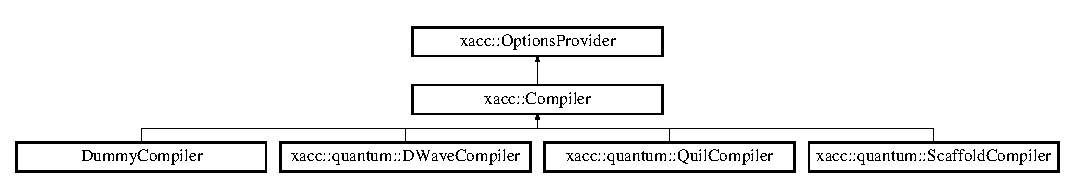
\includegraphics[height=2.079208cm]{a01451}
\end{center}
\end{figure}
\subsection*{Public Member Functions}
\begin{DoxyCompactItemize}
\item 
virtual std\+::shared\+\_\+ptr$<$ \hyperlink{a01499}{IR} $>$ \hyperlink{a01451_a546a40c95bb93af6a0c0ac48dbeaffc8}{compile} (const std\+::string \&src, std\+::shared\+\_\+ptr$<$ \hyperlink{a01435}{Accelerator} $>$ acc)=0
\item 
virtual std\+::shared\+\_\+ptr$<$ \hyperlink{a01499}{IR} $>$ \hyperlink{a01451_a9092f5f779b570c91569b59621280c04}{compile} (const std\+::string \&src)=0
\item 
virtual const std\+::string \hyperlink{a01451_aeedbe58a33fed29e4d7694ae743e25e7}{translate} (const std\+::string \&buffer\+Variable, std\+::shared\+\_\+ptr$<$ \hyperlink{a01475}{Function} $>$ function)=0
\item 
virtual const std\+::string \hyperlink{a01451_a87fca9100e6462122f5b687c3a0fb3fb}{get\+Name} ()=0
\item 
virtual std\+::shared\+\_\+ptr$<$ options\+\_\+description $>$ \hyperlink{a01451_a9f5a8965c9c2dd895016d18264ebbe92}{get\+Options} ()
\item 
virtual \hyperlink{a01451_a5d0b012687d9b44893872eaa81e47b38}{$\sim$\+Compiler} ()
\end{DoxyCompactItemize}
\subsection*{Protected Attributes}
\begin{DoxyCompactItemize}
\item 
std\+::string \hyperlink{a01451_a0ad81c816c09e5113d03cdc02165c453}{kernel\+Source}
\item 
std\+::shared\+\_\+ptr$<$ \hyperlink{a01435}{Accelerator} $>$ \hyperlink{a01451_ad4cbb467fa7e377bac6c054ffcb22b7c}{accelerator}
\end{DoxyCompactItemize}


\subsection{Detailed Description}
The \hyperlink{a01451}{Compiler} class provides an extensible interface for injecting custom compilation mechanisms into the X\+A\+CC framework. Implementations provide a compile method that takes the kernel source code string, performs compiler-\/specific compilation mechanism, and returns a valid X\+A\+CC \hyperlink{a01499}{IR} instance modeling the result of the compilation. 

\subsection{Constructor \& Destructor Documentation}
\mbox{\Hypertarget{a01451_a5d0b012687d9b44893872eaa81e47b38}\label{a01451_a5d0b012687d9b44893872eaa81e47b38}} 
\index{xacc\+::\+Compiler@{xacc\+::\+Compiler}!````~Compiler@{$\sim$\+Compiler}}
\index{````~Compiler@{$\sim$\+Compiler}!xacc\+::\+Compiler@{xacc\+::\+Compiler}}
\subsubsection{\texorpdfstring{$\sim$\+Compiler()}{~Compiler()}}
{\footnotesize\ttfamily virtual xacc\+::\+Compiler\+::$\sim$\+Compiler (\begin{DoxyParamCaption}{ }\end{DoxyParamCaption})\hspace{0.3cm}{\ttfamily [inline]}, {\ttfamily [virtual]}}

The destructor 

\subsection{Member Function Documentation}
\mbox{\Hypertarget{a01451_a546a40c95bb93af6a0c0ac48dbeaffc8}\label{a01451_a546a40c95bb93af6a0c0ac48dbeaffc8}} 
\index{xacc\+::\+Compiler@{xacc\+::\+Compiler}!compile@{compile}}
\index{compile@{compile}!xacc\+::\+Compiler@{xacc\+::\+Compiler}}
\subsubsection{\texorpdfstring{compile()}{compile()}\hspace{0.1cm}{\footnotesize\ttfamily [1/2]}}
{\footnotesize\ttfamily virtual std\+::shared\+\_\+ptr$<$\hyperlink{a01499}{IR}$>$ xacc\+::\+Compiler\+::compile (\begin{DoxyParamCaption}\item[{const std\+::string \&}]{src,  }\item[{std\+::shared\+\_\+ptr$<$ \hyperlink{a01435}{Accelerator} $>$}]{acc }\end{DoxyParamCaption})\hspace{0.3cm}{\ttfamily [pure virtual]}}

This method is to be implemented by derived Compilers and is in charge of executing the compilation mechanism on the provided source string. Implementations also are given access to the \hyperlink{a01435}{Accelerator} that this source code is intended for.


\begin{DoxyParams}{Parameters}
{\em src} & The kernel source string. \\
\hline
{\em acc} & The \hyperlink{a01435}{Accelerator} this code will be executed on \\
\hline
\end{DoxyParams}
\begin{DoxyReturn}{Returns}
ir Intermediate representation for provided source kernel code. 
\end{DoxyReturn}


Implemented in \hyperlink{a01103_a7caede75bb2304ba405966651b115543}{xacc\+::quantum\+::\+Scaffold\+Compiler}, \hyperlink{a01075_a2421482415ca4e09963ea4ecddff8100}{xacc\+::quantum\+::\+Quil\+Compiler}, \hyperlink{a01139_a9eaa6e6a4ff3645915d166a325bfde8d}{Dummy\+Compiler}, and \hyperlink{a01115_a0f7f6b10b4a881cb27b36eaa6d39e7b1}{xacc\+::quantum\+::\+D\+Wave\+Compiler}.

\mbox{\Hypertarget{a01451_a9092f5f779b570c91569b59621280c04}\label{a01451_a9092f5f779b570c91569b59621280c04}} 
\index{xacc\+::\+Compiler@{xacc\+::\+Compiler}!compile@{compile}}
\index{compile@{compile}!xacc\+::\+Compiler@{xacc\+::\+Compiler}}
\subsubsection{\texorpdfstring{compile()}{compile()}\hspace{0.1cm}{\footnotesize\ttfamily [2/2]}}
{\footnotesize\ttfamily virtual std\+::shared\+\_\+ptr$<$\hyperlink{a01499}{IR}$>$ xacc\+::\+Compiler\+::compile (\begin{DoxyParamCaption}\item[{const std\+::string \&}]{src }\end{DoxyParamCaption})\hspace{0.3cm}{\ttfamily [pure virtual]}}

This method is to be implemented by derived Compilers and is in charge of executing the compilation mechanism on the provided source string. 
\begin{DoxyParams}{Parameters}
{\em src} & \\
\hline
\end{DoxyParams}
\begin{DoxyReturn}{Returns}

\end{DoxyReturn}


Implemented in \hyperlink{a01103_a3736ecc229fe6acdd4c991e85d7a1f08}{xacc\+::quantum\+::\+Scaffold\+Compiler}, \hyperlink{a01075_adf4d321ecb0df3fa7728999f941c83b2}{xacc\+::quantum\+::\+Quil\+Compiler}, \hyperlink{a01139_a2f9bb3d30bb11f12b530854a11c8fb25}{Dummy\+Compiler}, and \hyperlink{a01115_a893e1d1c81a8aaf6e2435c9bceab575e}{xacc\+::quantum\+::\+D\+Wave\+Compiler}.

\mbox{\Hypertarget{a01451_a87fca9100e6462122f5b687c3a0fb3fb}\label{a01451_a87fca9100e6462122f5b687c3a0fb3fb}} 
\index{xacc\+::\+Compiler@{xacc\+::\+Compiler}!get\+Name@{get\+Name}}
\index{get\+Name@{get\+Name}!xacc\+::\+Compiler@{xacc\+::\+Compiler}}
\subsubsection{\texorpdfstring{get\+Name()}{getName()}}
{\footnotesize\ttfamily virtual const std\+::string xacc\+::\+Compiler\+::get\+Name (\begin{DoxyParamCaption}{ }\end{DoxyParamCaption})\hspace{0.3cm}{\ttfamily [pure virtual]}}

Return the name of this \hyperlink{a01451}{Compiler} \begin{DoxyReturn}{Returns}
name \hyperlink{a01451}{Compiler} name 
\end{DoxyReturn}


Implemented in \hyperlink{a01139_a76460cb78671dc2cf42f2bebf8fb80c7}{Dummy\+Compiler}, \hyperlink{a01103_a3f537054a3924a1d14f4ceb0f0181161}{xacc\+::quantum\+::\+Scaffold\+Compiler}, \hyperlink{a01075_ae7d52140b6dd52730edc6e38ae48f437}{xacc\+::quantum\+::\+Quil\+Compiler}, and \hyperlink{a01115_a8a180031ae563e1a9aac611e8066c181}{xacc\+::quantum\+::\+D\+Wave\+Compiler}.

\mbox{\Hypertarget{a01451_a9f5a8965c9c2dd895016d18264ebbe92}\label{a01451_a9f5a8965c9c2dd895016d18264ebbe92}} 
\index{xacc\+::\+Compiler@{xacc\+::\+Compiler}!get\+Options@{get\+Options}}
\index{get\+Options@{get\+Options}!xacc\+::\+Compiler@{xacc\+::\+Compiler}}
\subsubsection{\texorpdfstring{get\+Options()}{getOptions()}}
{\footnotesize\ttfamily virtual std\+::shared\+\_\+ptr$<$options\+\_\+description$>$ xacc\+::\+Compiler\+::get\+Options (\begin{DoxyParamCaption}{ }\end{DoxyParamCaption})\hspace{0.3cm}{\ttfamily [inline]}, {\ttfamily [virtual]}}

Return an empty options\+\_\+description, this is for subclasses to implement. 

Implements \hyperlink{a01543_a6d150954f852109bfe2c1ae90222926f}{xacc\+::\+Options\+Provider}.

\mbox{\Hypertarget{a01451_aeedbe58a33fed29e4d7694ae743e25e7}\label{a01451_aeedbe58a33fed29e4d7694ae743e25e7}} 
\index{xacc\+::\+Compiler@{xacc\+::\+Compiler}!translate@{translate}}
\index{translate@{translate}!xacc\+::\+Compiler@{xacc\+::\+Compiler}}
\subsubsection{\texorpdfstring{translate()}{translate()}}
{\footnotesize\ttfamily virtual const std\+::string xacc\+::\+Compiler\+::translate (\begin{DoxyParamCaption}\item[{const std\+::string \&}]{buffer\+Variable,  }\item[{std\+::shared\+\_\+ptr$<$ \hyperlink{a01475}{Function} $>$}]{function }\end{DoxyParamCaption})\hspace{0.3cm}{\ttfamily [pure virtual]}}

This method is to be implemented by derived Compilers and is in charge of taking the provided \hyperlink{a01475}{Function} \hyperlink{a01499}{IR} and converting it to source code in this \hyperlink{a01451}{Compiler}\textquotesingle{}s language.


\begin{DoxyParams}{Parameters}
{\em function} & The X\+A\+CC \hyperlink{a01499}{IR} \hyperlink{a01475}{Function} to translate \\
\hline
\end{DoxyParams}
\begin{DoxyReturn}{Returns}
src The source code as a string 
\end{DoxyReturn}


Implemented in \hyperlink{a01075_a66ca00bbb1f30e7bc6dd86b1e267b93b}{xacc\+::quantum\+::\+Quil\+Compiler}, \hyperlink{a01103_ac7ca2941e987ba579c6f50cfbd7fb0dc}{xacc\+::quantum\+::\+Scaffold\+Compiler}, \hyperlink{a01115_a73a8839c55d22c68e5264feca8d626d4}{xacc\+::quantum\+::\+D\+Wave\+Compiler}, and \hyperlink{a01139_a606c27150c8d374242b8824e45b1e0c1}{Dummy\+Compiler}.



\subsection{Member Data Documentation}
\mbox{\Hypertarget{a01451_ad4cbb467fa7e377bac6c054ffcb22b7c}\label{a01451_ad4cbb467fa7e377bac6c054ffcb22b7c}} 
\index{xacc\+::\+Compiler@{xacc\+::\+Compiler}!accelerator@{accelerator}}
\index{accelerator@{accelerator}!xacc\+::\+Compiler@{xacc\+::\+Compiler}}
\subsubsection{\texorpdfstring{accelerator}{accelerator}}
{\footnotesize\ttfamily std\+::shared\+\_\+ptr$<$\hyperlink{a01435}{Accelerator}$>$ xacc\+::\+Compiler\+::accelerator\hspace{0.3cm}{\ttfamily [protected]}}

Reference to the \hyperlink{a01435}{Accelerator} that this compiler is targeting. \mbox{\Hypertarget{a01451_a0ad81c816c09e5113d03cdc02165c453}\label{a01451_a0ad81c816c09e5113d03cdc02165c453}} 
\index{xacc\+::\+Compiler@{xacc\+::\+Compiler}!kernel\+Source@{kernel\+Source}}
\index{kernel\+Source@{kernel\+Source}!xacc\+::\+Compiler@{xacc\+::\+Compiler}}
\subsubsection{\texorpdfstring{kernel\+Source}{kernelSource}}
{\footnotesize\ttfamily std\+::string xacc\+::\+Compiler\+::kernel\+Source\hspace{0.3cm}{\ttfamily [protected]}}

Reference to the provided kernel source code string 

The documentation for this class was generated from the following file\+:\begin{DoxyCompactItemize}
\item 
Compiler.\+hpp\end{DoxyCompactItemize}

\hypertarget{a01179}{}\section{xacc\+:\+:quantum\+:\+:Conditional\+Function Class Reference}
\label{a01179}\index{xacc\+::quantum\+::\+Conditional\+Function@{xacc\+::quantum\+::\+Conditional\+Function}}
Inheritance diagram for xacc\+:\+:quantum\+:\+:Conditional\+Function\+:\begin{figure}[H]
\begin{center}
\leavevmode
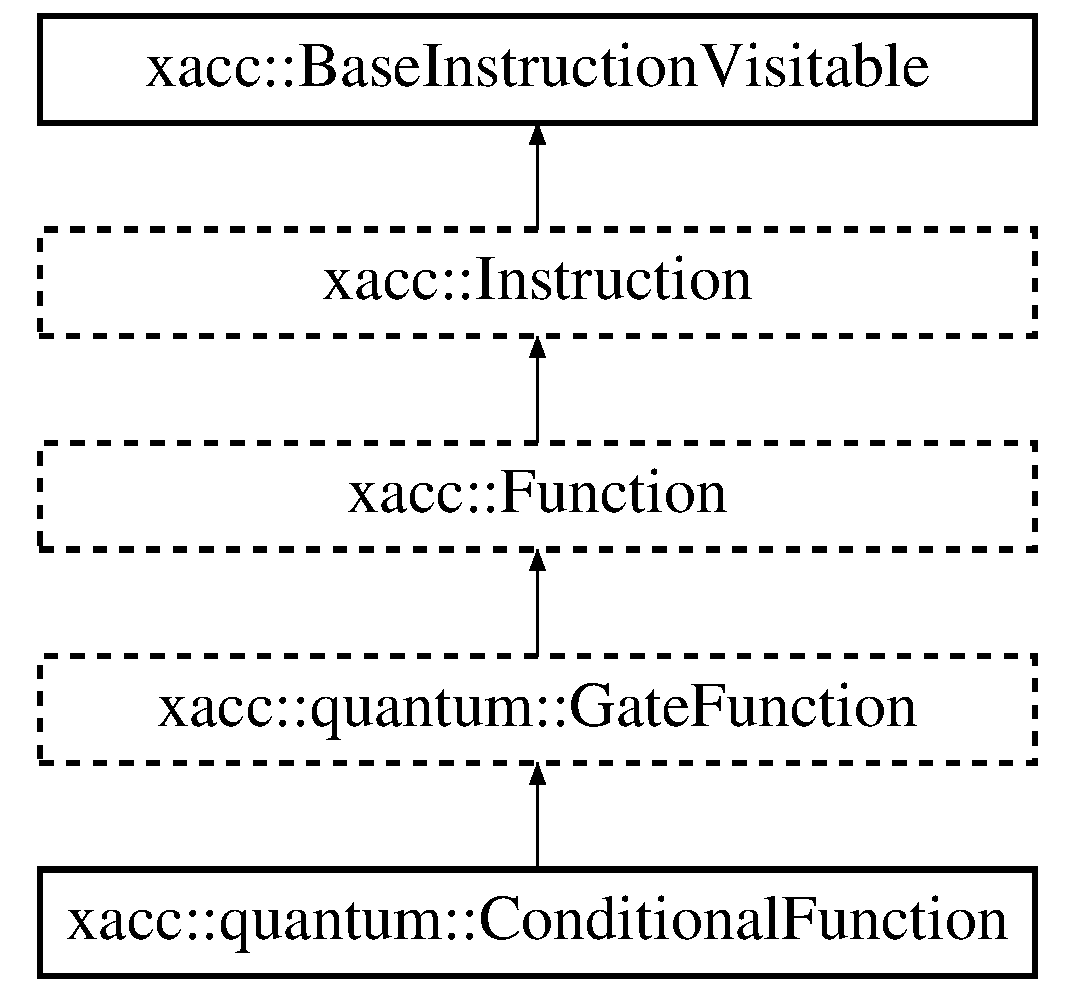
\includegraphics[height=5.000000cm]{a01179}
\end{center}
\end{figure}
\subsection*{Public Member Functions}
\begin{DoxyCompactItemize}
\item 
\mbox{\Hypertarget{a01179_aa28610a08ae04d62ccdd8359433100c3}\label{a01179_aa28610a08ae04d62ccdd8359433100c3}} 
{\bfseries Conditional\+Function} (int qbit)
\item 
virtual void \hyperlink{a01179_a6aedad20f96390880efdc0a476b3273f}{add\+Instruction} (Inst\+Ptr instruction)
\item 
\mbox{\Hypertarget{a01179_a804317333b6677a041a3071b5108c0df}\label{a01179_a804317333b6677a041a3071b5108c0df}} 
const int {\bfseries get\+Conditional\+Qubit} ()
\item 
\mbox{\Hypertarget{a01179_a709c236a5beb62d9a3bd5265196fb6c9}\label{a01179_a709c236a5beb62d9a3bd5265196fb6c9}} 
void {\bfseries evaluate} (const int acc\+Bit\+State)
\item 
virtual const std\+::string \hyperlink{a01179_aca7a5f849fece6fc28a904efee9a3370}{to\+String} (const std\+::string \&buffer\+Var\+Name)
\end{DoxyCompactItemize}
\subsection*{Protected Attributes}
\begin{DoxyCompactItemize}
\item 
\mbox{\Hypertarget{a01179_a0310536801417c0eded28a4dea1efa44}\label{a01179_a0310536801417c0eded28a4dea1efa44}} 
int {\bfseries qbit\+Idx}
\end{DoxyCompactItemize}
\subsection*{Additional Inherited Members}


\subsection{Member Function Documentation}
\mbox{\Hypertarget{a01179_a6aedad20f96390880efdc0a476b3273f}\label{a01179_a6aedad20f96390880efdc0a476b3273f}} 
\index{xacc\+::quantum\+::\+Conditional\+Function@{xacc\+::quantum\+::\+Conditional\+Function}!add\+Instruction@{add\+Instruction}}
\index{add\+Instruction@{add\+Instruction}!xacc\+::quantum\+::\+Conditional\+Function@{xacc\+::quantum\+::\+Conditional\+Function}}
\subsubsection{\texorpdfstring{add\+Instruction()}{addInstruction()}}
{\footnotesize\ttfamily void xacc\+::quantum\+::\+Conditional\+Function\+::add\+Instruction (\begin{DoxyParamCaption}\item[{Inst\+Ptr}]{instruction }\end{DoxyParamCaption})\hspace{0.3cm}{\ttfamily [virtual]}}

Add an instruction to this quantum intermediate representation.


\begin{DoxyParams}{Parameters}
{\em instruction} & \\
\hline
\end{DoxyParams}


Reimplemented from \hyperlink{a01155_a892fb69a10f0a7cb5abdab4cca61b80a}{xacc\+::quantum\+::\+Gate\+Function}.

\mbox{\Hypertarget{a01179_aca7a5f849fece6fc28a904efee9a3370}\label{a01179_aca7a5f849fece6fc28a904efee9a3370}} 
\index{xacc\+::quantum\+::\+Conditional\+Function@{xacc\+::quantum\+::\+Conditional\+Function}!to\+String@{to\+String}}
\index{to\+String@{to\+String}!xacc\+::quantum\+::\+Conditional\+Function@{xacc\+::quantum\+::\+Conditional\+Function}}
\subsubsection{\texorpdfstring{to\+String()}{toString()}}
{\footnotesize\ttfamily const std\+::string xacc\+::quantum\+::\+Conditional\+Function\+::to\+String (\begin{DoxyParamCaption}\item[{const std\+::string \&}]{buffer\+Var\+Name }\end{DoxyParamCaption})\hspace{0.3cm}{\ttfamily [virtual]}}

Return an assembly-\/like string representation for this function . 
\begin{DoxyParams}{Parameters}
{\em buffer\+Var\+Name} & \\
\hline
\end{DoxyParams}
\begin{DoxyReturn}{Returns}

\end{DoxyReturn}


Reimplemented from \hyperlink{a01155_aa1950776ae84bad2d0795a0441f910e7}{xacc\+::quantum\+::\+Gate\+Function}.



The documentation for this class was generated from the following files\+:\begin{DoxyCompactItemize}
\item 
Conditional\+Function.\+hpp\item 
Conditional\+Function.\+cpp\end{DoxyCompactItemize}

\hypertarget{a01411}{}\section{C\+Simple\+Ini\+Templ$<$ S\+I\+\_\+\+C\+H\+AR, S\+I\+\_\+\+S\+T\+R\+L\+E\+SS, S\+I\+\_\+\+C\+O\+N\+V\+E\+R\+T\+ER $>$\+:\+:Converter Class Reference}
\label{a01411}\index{C\+Simple\+Ini\+Templ$<$ S\+I\+\_\+\+C\+H\+A\+R, S\+I\+\_\+\+S\+T\+R\+L\+E\+S\+S, S\+I\+\_\+\+C\+O\+N\+V\+E\+R\+T\+E\+R $>$\+::\+Converter@{C\+Simple\+Ini\+Templ$<$ S\+I\+\_\+\+C\+H\+A\+R, S\+I\+\_\+\+S\+T\+R\+L\+E\+S\+S, S\+I\+\_\+\+C\+O\+N\+V\+E\+R\+T\+E\+R $>$\+::\+Converter}}


{\ttfamily \#include $<$Simple\+Ini.\+h$>$}

Inheritance diagram for C\+Simple\+Ini\+Templ$<$ S\+I\+\_\+\+C\+H\+AR, S\+I\+\_\+\+S\+T\+R\+L\+E\+SS, S\+I\+\_\+\+C\+O\+N\+V\+E\+R\+T\+ER $>$\+:\+:Converter\+:\begin{figure}[H]
\begin{center}
\leavevmode
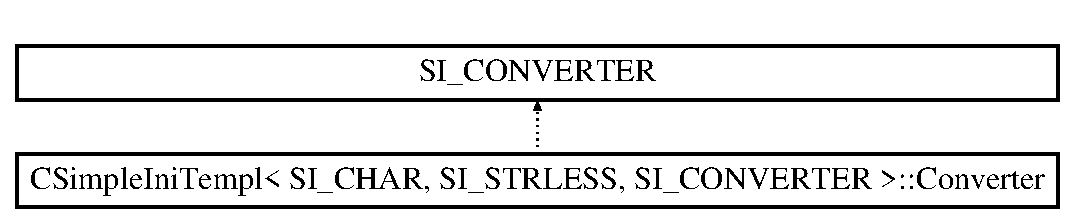
\includegraphics[height=2.000000cm]{a01411}
\end{center}
\end{figure}
\subsection*{Public Member Functions}
\begin{DoxyCompactItemize}
\item 
\mbox{\Hypertarget{a01411_ab8e740b211e4ece127d4d25773ba7e42}\label{a01411_ab8e740b211e4ece127d4d25773ba7e42}} 
{\bfseries Converter} (bool a\+\_\+b\+Store\+Is\+Utf8)
\item 
\mbox{\Hypertarget{a01411_a2f6e993014ed5d60c6e890e55beb0805}\label{a01411_a2f6e993014ed5d60c6e890e55beb0805}} 
{\bfseries Converter} (const \hyperlink{a01411}{Converter} \&rhs)
\item 
\mbox{\Hypertarget{a01411_af858c01c6a7e4ce9fafd18abc9e0ac1b}\label{a01411_af858c01c6a7e4ce9fafd18abc9e0ac1b}} 
\hyperlink{a01411}{Converter} \& {\bfseries operator=} (const \hyperlink{a01411}{Converter} \&rhs)
\item 
\mbox{\Hypertarget{a01411_a4e4186867214b54326cf622e323c9f2f}\label{a01411_a4e4186867214b54326cf622e323c9f2f}} 
bool {\bfseries Convert\+To\+Store} (const S\+I\+\_\+\+C\+H\+AR $\ast$a\+\_\+psz\+String)
\item 
\mbox{\Hypertarget{a01411_a918bbd4f861a2872e148bc9481ac80bb}\label{a01411_a918bbd4f861a2872e148bc9481ac80bb}} 
const char $\ast$ {\bfseries Data} ()
\end{DoxyCompactItemize}


\subsection{Detailed Description}
\subsubsection*{template$<$class S\+I\+\_\+\+C\+H\+AR, class S\+I\+\_\+\+S\+T\+R\+L\+E\+SS, class S\+I\+\_\+\+C\+O\+N\+V\+E\+R\+T\+ER$>$\newline
class C\+Simple\+Ini\+Templ$<$ S\+I\+\_\+\+C\+H\+A\+R, S\+I\+\_\+\+S\+T\+R\+L\+E\+S\+S, S\+I\+\_\+\+C\+O\+N\+V\+E\+R\+T\+E\+R $>$\+::\+Converter}

Characterset conversion utility class to convert strings to the same format as is used for the storage. 

The documentation for this class was generated from the following file\+:\begin{DoxyCompactItemize}
\item 
Simple\+Ini.\+h\end{DoxyCompactItemize}

\hypertarget{a01091}{}\section{Count\+Gate\+Visitor$<$ Gate\+Type $>$ Class Template Reference}
\label{a01091}\index{Count\+Gate\+Visitor$<$ Gate\+Type $>$@{Count\+Gate\+Visitor$<$ Gate\+Type $>$}}
Inheritance diagram for Count\+Gate\+Visitor$<$ Gate\+Type $>$\+:\begin{figure}[H]
\begin{center}
\leavevmode
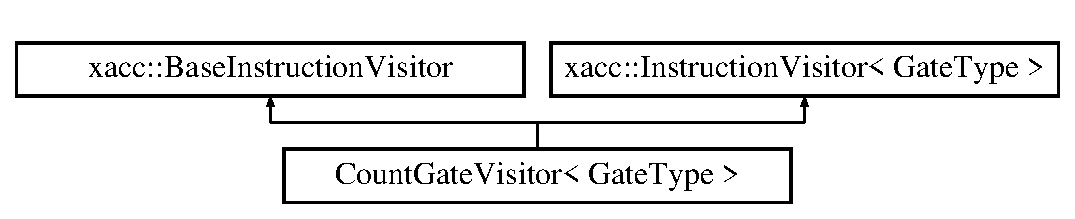
\includegraphics[height=2.000000cm]{a01091}
\end{center}
\end{figure}
\subsection*{Public Member Functions}
\begin{DoxyCompactItemize}
\item 
virtual void \hyperlink{a01091_a144f1e4e6d24c450e0a941fa650c1f48}{visit} (Gate\+Type \&gate)
\end{DoxyCompactItemize}
\subsection*{Public Attributes}
\begin{DoxyCompactItemize}
\item 
\mbox{\Hypertarget{a01091_a74c1ba58befe42d9dbdbd5eb14aa46ca}\label{a01091_a74c1ba58befe42d9dbdbd5eb14aa46ca}} 
int {\bfseries count} = 0
\end{DoxyCompactItemize}


\subsection{Member Function Documentation}
\mbox{\Hypertarget{a01091_a144f1e4e6d24c450e0a941fa650c1f48}\label{a01091_a144f1e4e6d24c450e0a941fa650c1f48}} 
\index{Count\+Gate\+Visitor@{Count\+Gate\+Visitor}!visit@{visit}}
\index{visit@{visit}!Count\+Gate\+Visitor@{Count\+Gate\+Visitor}}
\subsubsection{\texorpdfstring{visit()}{visit()}}
{\footnotesize\ttfamily template$<$typename Gate\+Type $>$ \\
virtual void \hyperlink{a01091}{Count\+Gate\+Visitor}$<$ Gate\+Type $>$\+::visit (\begin{DoxyParamCaption}\item[{Gate\+Type \&}]{ }\end{DoxyParamCaption})\hspace{0.3cm}{\ttfamily [inline]}, {\ttfamily [virtual]}}

This method should be implemented by subclasses to perform Visitor-\/specific behavior on the given instance of the template parameter T. 

Implements \hyperlink{a01491_af0fead298f5bfbb8e6680433063e2c4b}{xacc\+::\+Instruction\+Visitor$<$ Gate\+Type $>$}.



The documentation for this class was generated from the following file\+:\begin{DoxyCompactItemize}
\item 
Quil\+Compiler\+Tester.\+cpp\end{DoxyCompactItemize}

\hypertarget{a01183}{}\section{xacc\+:\+:int\+\_\+$<$ size\+\_\+t $>$ Struct Template Reference}
\label{a01183}\index{xacc\+::int\+\_\+$<$ size\+\_\+t $>$@{xacc\+::int\+\_\+$<$ size\+\_\+t $>$}}


The documentation for this struct was generated from the following file\+:\begin{DoxyCompactItemize}
\item 
Graph.\+hpp\end{DoxyCompactItemize}

\hypertarget{a01383}{}\section{C\+Simple\+Ini\+Templ$<$ S\+I\+\_\+\+C\+H\+AR, S\+I\+\_\+\+S\+T\+R\+L\+E\+SS, S\+I\+\_\+\+C\+O\+N\+V\+E\+R\+T\+ER $>$ Class Template Reference}
\label{a01383}\index{C\+Simple\+Ini\+Templ$<$ S\+I\+\_\+\+C\+H\+A\+R, S\+I\+\_\+\+S\+T\+R\+L\+E\+S\+S, S\+I\+\_\+\+C\+O\+N\+V\+E\+R\+T\+E\+R $>$@{C\+Simple\+Ini\+Templ$<$ S\+I\+\_\+\+C\+H\+A\+R, S\+I\+\_\+\+S\+T\+R\+L\+E\+S\+S, S\+I\+\_\+\+C\+O\+N\+V\+E\+R\+T\+E\+R $>$}}


{\ttfamily \#include $<$Simple\+Ini.\+h$>$}

\subsection*{Classes}
\begin{DoxyCompactItemize}
\item 
class \hyperlink{a01411}{Converter}
\item 
struct \hyperlink{a01387}{Entry}
\item 
class \hyperlink{a01403}{File\+Writer}
\item 
class \hyperlink{a01399}{Output\+Writer}
\item 
class \hyperlink{a01407}{String\+Writer}
\end{DoxyCompactItemize}
\subsection*{Public Types}
\begin{DoxyCompactItemize}
\item 
\mbox{\Hypertarget{a01383_ad7ffad7e87da2303a05b885e95bc74fa}\label{a01383_ad7ffad7e87da2303a05b885e95bc74fa}} 
typedef S\+I\+\_\+\+C\+H\+AR {\bfseries S\+I\+\_\+\+C\+H\+A\+R\+\_\+T}
\item 
typedef std\+::multimap$<$ \hyperlink{a01387}{Entry}, const S\+I\+\_\+\+C\+H\+AR $\ast$, typename \hyperlink{a01391}{Entry\+::\+Key\+Order} $>$ \hyperlink{a01383_ae7f0e11d84617214bd479de6332c80e6}{T\+Key\+Val}
\item 
typedef std\+::map$<$ \hyperlink{a01387}{Entry}, \hyperlink{a01383_ae7f0e11d84617214bd479de6332c80e6}{T\+Key\+Val}, typename \hyperlink{a01391}{Entry\+::\+Key\+Order} $>$ \hyperlink{a01383_a2e7963455f680abd0d6901786495a665}{T\+Section}
\item 
typedef std\+::list$<$ \hyperlink{a01387}{Entry} $>$ \hyperlink{a01383_a391b3f3751e06cd9e9de4fb16ac14342}{T\+Names\+Depend}
\end{DoxyCompactItemize}
\subsection*{Public Member Functions}
\begin{DoxyCompactItemize}
\item 
\hyperlink{a01383_af878d0a2aa780255b621e95f58f691d8}{C\+Simple\+Ini\+Templ} (bool a\+\_\+b\+Is\+Utf8=false, bool a\+\_\+b\+Multi\+Key=false, bool a\+\_\+b\+Multi\+Line=false)
\item 
\hyperlink{a01383_a8c933adc1d46bb663caeb6f9dee5aa12}{$\sim$\+C\+Simple\+Ini\+Templ} ()
\item 
void \hyperlink{a01383_a89b34d38be4518e9ed91c634a41b8055}{Reset} ()
\item 
bool \hyperlink{a01383_a54bbe9727db17b368a0a75abd5e52d1c}{Is\+Empty} () const
\item 
S\+I\+\_\+\+Error \hyperlink{a01383_aebb6e5fff76efc05ca6cc4b7b56481a3}{Load\+File} (const char $\ast$a\+\_\+psz\+File)
\item 
S\+I\+\_\+\+Error \hyperlink{a01383_a7ccb65e82fa347b42b59330968f826ae}{Load\+File} (F\+I\+LE $\ast$a\+\_\+fp\+File)
\item 
S\+I\+\_\+\+Error \hyperlink{a01383_a174244fd3e09ff78da05fe46be86e714}{Load\+Data} (const std\+::string \&a\+\_\+str\+Data)
\item 
S\+I\+\_\+\+Error \hyperlink{a01383_aa797cf47cec05906f07d5065882af4d3}{Load\+Data} (const char $\ast$a\+\_\+p\+Data, size\+\_\+t a\+\_\+u\+Data\+Len)
\item 
S\+I\+\_\+\+Error \hyperlink{a01383_af00e754689a94cbe87b387f99f7a5d01}{Save\+File} (const char $\ast$a\+\_\+psz\+File, bool a\+\_\+b\+Add\+Signature=true) const
\item 
S\+I\+\_\+\+Error \hyperlink{a01383_a3c3f677c1515e08751cb52a1dfaf1a93}{Save\+File} (F\+I\+LE $\ast$a\+\_\+p\+File, bool a\+\_\+b\+Add\+Signature=false) const
\item 
S\+I\+\_\+\+Error \hyperlink{a01383_a6ec10daab297e92cdffe024ba5e6d999}{Save} (\hyperlink{a01399}{Output\+Writer} \&a\+\_\+o\+Output, bool a\+\_\+b\+Add\+Signature=false) const
\item 
S\+I\+\_\+\+Error \hyperlink{a01383_a9fc5894f12a31b8496a9627cd0f42139}{Save} (std\+::string \&a\+\_\+s\+Buffer, bool a\+\_\+b\+Add\+Signature=false) const
\item 
void \hyperlink{a01383_a7fe8a8b70b0ef000c591011a8332ebd5}{Get\+All\+Sections} (\hyperlink{a01383_a391b3f3751e06cd9e9de4fb16ac14342}{T\+Names\+Depend} \&a\+\_\+names) const
\item 
bool \hyperlink{a01383_a08cadb6624a6c459703efaadb25d31c9}{Get\+All\+Keys} (const S\+I\+\_\+\+C\+H\+AR $\ast$a\+\_\+p\+Section, \hyperlink{a01383_a391b3f3751e06cd9e9de4fb16ac14342}{T\+Names\+Depend} \&a\+\_\+names) const
\item 
bool \hyperlink{a01383_adda5ee7f422695f7e67be2d066e303bf}{Get\+All\+Values} (const S\+I\+\_\+\+C\+H\+AR $\ast$a\+\_\+p\+Section, const S\+I\+\_\+\+C\+H\+AR $\ast$a\+\_\+p\+Key, \hyperlink{a01383_a391b3f3751e06cd9e9de4fb16ac14342}{T\+Names\+Depend} \&a\+\_\+values) const
\item 
int \hyperlink{a01383_a0a9c089eabb5faf764c4af449f7b1846}{Get\+Section\+Size} (const S\+I\+\_\+\+C\+H\+AR $\ast$a\+\_\+p\+Section) const
\item 
const \hyperlink{a01383_ae7f0e11d84617214bd479de6332c80e6}{T\+Key\+Val} $\ast$ \hyperlink{a01383_a56a6838556328ab8bfaa7ded9edb9c8a}{Get\+Section} (const S\+I\+\_\+\+C\+H\+AR $\ast$a\+\_\+p\+Section) const
\item 
const S\+I\+\_\+\+C\+H\+AR $\ast$ \hyperlink{a01383_a74e3f5d22f50b70b2a20c89ec7e2c737}{Get\+Value} (const S\+I\+\_\+\+C\+H\+AR $\ast$a\+\_\+p\+Section, const S\+I\+\_\+\+C\+H\+AR $\ast$a\+\_\+p\+Key, const S\+I\+\_\+\+C\+H\+AR $\ast$a\+\_\+p\+Default=N\+U\+LL, bool $\ast$a\+\_\+p\+Has\+Multiple=N\+U\+LL) const
\item 
long \hyperlink{a01383_a7fa211c1c768497520eab7f2014ae786}{Get\+Long\+Value} (const S\+I\+\_\+\+C\+H\+AR $\ast$a\+\_\+p\+Section, const S\+I\+\_\+\+C\+H\+AR $\ast$a\+\_\+p\+Key, long a\+\_\+n\+Default=0, bool $\ast$a\+\_\+p\+Has\+Multiple=N\+U\+LL) const
\item 
double \hyperlink{a01383_aab58a949481926cf1d42fcbf9552d77b}{Get\+Double\+Value} (const S\+I\+\_\+\+C\+H\+AR $\ast$a\+\_\+p\+Section, const S\+I\+\_\+\+C\+H\+AR $\ast$a\+\_\+p\+Key, double a\+\_\+n\+Default=0, bool $\ast$a\+\_\+p\+Has\+Multiple=N\+U\+LL) const
\item 
bool \hyperlink{a01383_a76b3165ce01224f82daee5ef63b3c96d}{Get\+Bool\+Value} (const S\+I\+\_\+\+C\+H\+AR $\ast$a\+\_\+p\+Section, const S\+I\+\_\+\+C\+H\+AR $\ast$a\+\_\+p\+Key, bool a\+\_\+b\+Default=false, bool $\ast$a\+\_\+p\+Has\+Multiple=N\+U\+LL) const
\item 
S\+I\+\_\+\+Error \hyperlink{a01383_aa2014a3dc8fdd638316cf1d3611796ab}{Set\+Value} (const S\+I\+\_\+\+C\+H\+AR $\ast$a\+\_\+p\+Section, const S\+I\+\_\+\+C\+H\+AR $\ast$a\+\_\+p\+Key, const S\+I\+\_\+\+C\+H\+AR $\ast$a\+\_\+p\+Value, const S\+I\+\_\+\+C\+H\+AR $\ast$a\+\_\+p\+Comment=N\+U\+LL, bool a\+\_\+b\+Force\+Replace=false)
\item 
S\+I\+\_\+\+Error \hyperlink{a01383_ab2238be407232e4bba0f1343e4793e4e}{Set\+Long\+Value} (const S\+I\+\_\+\+C\+H\+AR $\ast$a\+\_\+p\+Section, const S\+I\+\_\+\+C\+H\+AR $\ast$a\+\_\+p\+Key, long a\+\_\+n\+Value, const S\+I\+\_\+\+C\+H\+AR $\ast$a\+\_\+p\+Comment=N\+U\+LL, bool a\+\_\+b\+Use\+Hex=false, bool a\+\_\+b\+Force\+Replace=false)
\item 
S\+I\+\_\+\+Error \hyperlink{a01383_af92ba0b8067553ab693c62a370de6534}{Set\+Double\+Value} (const S\+I\+\_\+\+C\+H\+AR $\ast$a\+\_\+p\+Section, const S\+I\+\_\+\+C\+H\+AR $\ast$a\+\_\+p\+Key, double a\+\_\+n\+Value, const S\+I\+\_\+\+C\+H\+AR $\ast$a\+\_\+p\+Comment=N\+U\+LL, bool a\+\_\+b\+Force\+Replace=false)
\item 
S\+I\+\_\+\+Error \hyperlink{a01383_a48ae136fa20c5d7eb7ab0b75342b27cf}{Set\+Bool\+Value} (const S\+I\+\_\+\+C\+H\+AR $\ast$a\+\_\+p\+Section, const S\+I\+\_\+\+C\+H\+AR $\ast$a\+\_\+p\+Key, bool a\+\_\+b\+Value, const S\+I\+\_\+\+C\+H\+AR $\ast$a\+\_\+p\+Comment=N\+U\+LL, bool a\+\_\+b\+Force\+Replace=false)
\item 
bool \hyperlink{a01383_aa5c1cdd0b306434d9e9f1422888049da}{Delete} (const S\+I\+\_\+\+C\+H\+AR $\ast$a\+\_\+p\+Section, const S\+I\+\_\+\+C\+H\+AR $\ast$a\+\_\+p\+Key, bool a\+\_\+b\+Remove\+Empty=false)
\item 
\hyperlink{a01411}{Converter} \hyperlink{a01383_a4a48496d4e4840a2254a9e31e16eaf6d}{Get\+Converter} () const
\end{DoxyCompactItemize}
\begin{Indent}\textbf{ Settings}\par
\begin{DoxyCompactItemize}
\item 
void \hyperlink{a01383_aa9a15a66de893571014f661f89cb4d4b}{Set\+Unicode} (bool a\+\_\+b\+Is\+Utf8=true)
\item 
bool \hyperlink{a01383_a40b4ee04251bd343ada5c4a4c508cd43}{Is\+Unicode} () const
\item 
void \hyperlink{a01383_ac3cfaf072a64f960bdcb7ddf2edc52b6}{Set\+Multi\+Key} (bool a\+\_\+b\+Allow\+Multi\+Key=true)
\item 
bool \hyperlink{a01383_a494b30fbdda5e78afdb25451743df935}{Is\+Multi\+Key} () const
\item 
void \hyperlink{a01383_aa7214b76600790053a5c715e9730aab0}{Set\+Multi\+Line} (bool a\+\_\+b\+Allow\+Multi\+Line=true)
\item 
bool \hyperlink{a01383_afadd3818363ec7e66ca369ef486ec979}{Is\+Multi\+Line} () const
\item 
void \hyperlink{a01383_ae3c0eae2dcd84a42c99bb86ae103662c}{Set\+Spaces} (bool a\+\_\+b\+Spaces=true)
\item 
bool \hyperlink{a01383_a92203e0c21f8d71e5d1621a18ee0be50}{Using\+Spaces} () const
\end{DoxyCompactItemize}
\end{Indent}


\subsection{Detailed Description}
\subsubsection*{template$<$class S\+I\+\_\+\+C\+H\+AR, class S\+I\+\_\+\+S\+T\+R\+L\+E\+SS, class S\+I\+\_\+\+C\+O\+N\+V\+E\+R\+T\+ER$>$\newline
class C\+Simple\+Ini\+Templ$<$ S\+I\+\_\+\+C\+H\+A\+R, S\+I\+\_\+\+S\+T\+R\+L\+E\+S\+S, S\+I\+\_\+\+C\+O\+N\+V\+E\+R\+T\+E\+R $>$}

Simple I\+NI file reader.

This can be instantiated with the choice of unicode or native characterset, and case sensitive or insensitive comparisons of section and key names. The supported combinations are pre-\/defined with the following typedefs\+:

\tabulinesep=1mm
\begin{longtabu} spread 0pt [c]{*{3}{|X[-1]}|}
\hline
\rowcolor{\tableheadbgcolor}\textbf{ Interface }&\textbf{ Case-\/sensitive }&\textbf{ Typedef }\\\cline{1-3}
\endfirsthead
\hline
\endfoot
\hline
\rowcolor{\tableheadbgcolor}\textbf{ Interface }&\textbf{ Case-\/sensitive }&\textbf{ Typedef }\\\cline{1-3}
\endhead
char &No &C\+Simple\+IniA \\\cline{1-3}
char &Yes &C\+Simple\+Ini\+CaseA \\\cline{1-3}
wchar\+\_\+t &No &C\+Simple\+IniW \\\cline{1-3}
wchar\+\_\+t &Yes &C\+Simple\+Ini\+CaseW \\\cline{1-3}
\end{longtabu}


Note that using other types for the S\+I\+\_\+\+C\+H\+AR is supported. For instance, unsigned char, unsigned short, etc. Note that where the alternative type is a different size to char/wchar\+\_\+t you may need to supply new helper classes for S\+I\+\_\+\+S\+T\+R\+L\+E\+SS and S\+I\+\_\+\+C\+O\+N\+V\+E\+R\+T\+ER. 

\subsection{Member Typedef Documentation}
\mbox{\Hypertarget{a01383_ae7f0e11d84617214bd479de6332c80e6}\label{a01383_ae7f0e11d84617214bd479de6332c80e6}} 
\index{C\+Simple\+Ini\+Templ@{C\+Simple\+Ini\+Templ}!T\+Key\+Val@{T\+Key\+Val}}
\index{T\+Key\+Val@{T\+Key\+Val}!C\+Simple\+Ini\+Templ@{C\+Simple\+Ini\+Templ}}
\subsubsection{\texorpdfstring{T\+Key\+Val}{TKeyVal}}
{\footnotesize\ttfamily template$<$class S\+I\+\_\+\+C\+H\+AR , class S\+I\+\_\+\+S\+T\+R\+L\+E\+SS , class S\+I\+\_\+\+C\+O\+N\+V\+E\+R\+T\+ER $>$ \\
typedef std\+::multimap$<$\hyperlink{a01387}{Entry},const S\+I\+\_\+\+C\+H\+AR $\ast$,typename \hyperlink{a01391}{Entry\+::\+Key\+Order}$>$ \hyperlink{a01383}{C\+Simple\+Ini\+Templ}$<$ S\+I\+\_\+\+C\+H\+AR, S\+I\+\_\+\+S\+T\+R\+L\+E\+SS, S\+I\+\_\+\+C\+O\+N\+V\+E\+R\+T\+ER $>$\+::\hyperlink{a01383_ae7f0e11d84617214bd479de6332c80e6}{T\+Key\+Val}}

map keys to values \mbox{\Hypertarget{a01383_a391b3f3751e06cd9e9de4fb16ac14342}\label{a01383_a391b3f3751e06cd9e9de4fb16ac14342}} 
\index{C\+Simple\+Ini\+Templ@{C\+Simple\+Ini\+Templ}!T\+Names\+Depend@{T\+Names\+Depend}}
\index{T\+Names\+Depend@{T\+Names\+Depend}!C\+Simple\+Ini\+Templ@{C\+Simple\+Ini\+Templ}}
\subsubsection{\texorpdfstring{T\+Names\+Depend}{TNamesDepend}}
{\footnotesize\ttfamily template$<$class S\+I\+\_\+\+C\+H\+AR , class S\+I\+\_\+\+S\+T\+R\+L\+E\+SS , class S\+I\+\_\+\+C\+O\+N\+V\+E\+R\+T\+ER $>$ \\
typedef std\+::list$<$\hyperlink{a01387}{Entry}$>$ \hyperlink{a01383}{C\+Simple\+Ini\+Templ}$<$ S\+I\+\_\+\+C\+H\+AR, S\+I\+\_\+\+S\+T\+R\+L\+E\+SS, S\+I\+\_\+\+C\+O\+N\+V\+E\+R\+T\+ER $>$\+::\hyperlink{a01383_a391b3f3751e06cd9e9de4fb16ac14342}{T\+Names\+Depend}}

set of dependent string pointers. Note that these pointers are dependent on memory owned by C\+Simple\+Ini. \mbox{\Hypertarget{a01383_a2e7963455f680abd0d6901786495a665}\label{a01383_a2e7963455f680abd0d6901786495a665}} 
\index{C\+Simple\+Ini\+Templ@{C\+Simple\+Ini\+Templ}!T\+Section@{T\+Section}}
\index{T\+Section@{T\+Section}!C\+Simple\+Ini\+Templ@{C\+Simple\+Ini\+Templ}}
\subsubsection{\texorpdfstring{T\+Section}{TSection}}
{\footnotesize\ttfamily template$<$class S\+I\+\_\+\+C\+H\+AR , class S\+I\+\_\+\+S\+T\+R\+L\+E\+SS , class S\+I\+\_\+\+C\+O\+N\+V\+E\+R\+T\+ER $>$ \\
typedef std\+::map$<$\hyperlink{a01387}{Entry},\hyperlink{a01383_ae7f0e11d84617214bd479de6332c80e6}{T\+Key\+Val},typename \hyperlink{a01391}{Entry\+::\+Key\+Order}$>$ \hyperlink{a01383}{C\+Simple\+Ini\+Templ}$<$ S\+I\+\_\+\+C\+H\+AR, S\+I\+\_\+\+S\+T\+R\+L\+E\+SS, S\+I\+\_\+\+C\+O\+N\+V\+E\+R\+T\+ER $>$\+::\hyperlink{a01383_a2e7963455f680abd0d6901786495a665}{T\+Section}}

map sections to key/value map 

\subsection{Constructor \& Destructor Documentation}
\mbox{\Hypertarget{a01383_af878d0a2aa780255b621e95f58f691d8}\label{a01383_af878d0a2aa780255b621e95f58f691d8}} 
\index{C\+Simple\+Ini\+Templ@{C\+Simple\+Ini\+Templ}!C\+Simple\+Ini\+Templ@{C\+Simple\+Ini\+Templ}}
\index{C\+Simple\+Ini\+Templ@{C\+Simple\+Ini\+Templ}!C\+Simple\+Ini\+Templ@{C\+Simple\+Ini\+Templ}}
\subsubsection{\texorpdfstring{C\+Simple\+Ini\+Templ()}{CSimpleIniTempl()}}
{\footnotesize\ttfamily template$<$class S\+I\+\_\+\+C\+H\+AR , class S\+I\+\_\+\+S\+T\+R\+L\+E\+SS , class S\+I\+\_\+\+C\+O\+N\+V\+E\+R\+T\+ER $>$ \\
\hyperlink{a01383}{C\+Simple\+Ini\+Templ}$<$ S\+I\+\_\+\+C\+H\+AR, S\+I\+\_\+\+S\+T\+R\+L\+E\+SS, S\+I\+\_\+\+C\+O\+N\+V\+E\+R\+T\+ER $>$\+::\hyperlink{a01383}{C\+Simple\+Ini\+Templ} (\begin{DoxyParamCaption}\item[{bool}]{a\+\_\+b\+Is\+Utf8 = {\ttfamily false},  }\item[{bool}]{a\+\_\+b\+Multi\+Key = {\ttfamily false},  }\item[{bool}]{a\+\_\+b\+Multi\+Line = {\ttfamily false} }\end{DoxyParamCaption})}

Default constructor.


\begin{DoxyParams}{Parameters}
{\em a\+\_\+b\+Is\+Utf8} & See the method \hyperlink{a01383_aa9a15a66de893571014f661f89cb4d4b}{Set\+Unicode()} for details. \\
\hline
{\em a\+\_\+b\+Multi\+Key} & See the method \hyperlink{a01383_ac3cfaf072a64f960bdcb7ddf2edc52b6}{Set\+Multi\+Key()} for details. \\
\hline
{\em a\+\_\+b\+Multi\+Line} & See the method \hyperlink{a01383_aa7214b76600790053a5c715e9730aab0}{Set\+Multi\+Line()} for details. \\
\hline
\end{DoxyParams}
\mbox{\Hypertarget{a01383_a8c933adc1d46bb663caeb6f9dee5aa12}\label{a01383_a8c933adc1d46bb663caeb6f9dee5aa12}} 
\index{C\+Simple\+Ini\+Templ@{C\+Simple\+Ini\+Templ}!````~C\+Simple\+Ini\+Templ@{$\sim$\+C\+Simple\+Ini\+Templ}}
\index{````~C\+Simple\+Ini\+Templ@{$\sim$\+C\+Simple\+Ini\+Templ}!C\+Simple\+Ini\+Templ@{C\+Simple\+Ini\+Templ}}
\subsubsection{\texorpdfstring{$\sim$\+C\+Simple\+Ini\+Templ()}{~CSimpleIniTempl()}}
{\footnotesize\ttfamily template$<$class S\+I\+\_\+\+C\+H\+AR , class S\+I\+\_\+\+S\+T\+R\+L\+E\+SS , class S\+I\+\_\+\+C\+O\+N\+V\+E\+R\+T\+ER $>$ \\
\hyperlink{a01383}{C\+Simple\+Ini\+Templ}$<$ S\+I\+\_\+\+C\+H\+AR, S\+I\+\_\+\+S\+T\+R\+L\+E\+SS, S\+I\+\_\+\+C\+O\+N\+V\+E\+R\+T\+ER $>$\+::$\sim$\hyperlink{a01383}{C\+Simple\+Ini\+Templ} (\begin{DoxyParamCaption}{ }\end{DoxyParamCaption})}

Destructor 

\subsection{Member Function Documentation}
\mbox{\Hypertarget{a01383_aa5c1cdd0b306434d9e9f1422888049da}\label{a01383_aa5c1cdd0b306434d9e9f1422888049da}} 
\index{C\+Simple\+Ini\+Templ@{C\+Simple\+Ini\+Templ}!Delete@{Delete}}
\index{Delete@{Delete}!C\+Simple\+Ini\+Templ@{C\+Simple\+Ini\+Templ}}
\subsubsection{\texorpdfstring{Delete()}{Delete()}}
{\footnotesize\ttfamily template$<$class S\+I\+\_\+\+C\+H\+AR , class S\+I\+\_\+\+S\+T\+R\+L\+E\+SS , class S\+I\+\_\+\+C\+O\+N\+V\+E\+R\+T\+ER $>$ \\
bool \hyperlink{a01383}{C\+Simple\+Ini\+Templ}$<$ S\+I\+\_\+\+C\+H\+AR, S\+I\+\_\+\+S\+T\+R\+L\+E\+SS, S\+I\+\_\+\+C\+O\+N\+V\+E\+R\+T\+ER $>$\+::Delete (\begin{DoxyParamCaption}\item[{const S\+I\+\_\+\+C\+H\+AR $\ast$}]{a\+\_\+p\+Section,  }\item[{const S\+I\+\_\+\+C\+H\+AR $\ast$}]{a\+\_\+p\+Key,  }\item[{bool}]{a\+\_\+b\+Remove\+Empty = {\ttfamily false} }\end{DoxyParamCaption})}

Delete an entire section, or a key from a section. Note that the data returned by Get\+Section is invalid and must not be used after anything has been deleted from that section using this method. Note when multiple keys is enabled, this will delete all keys with that name; there is no way to selectively delete individual key/values in this situation.


\begin{DoxyParams}{Parameters}
{\em a\+\_\+p\+Section} & Section to delete key from, or if a\+\_\+p\+Key is N\+U\+LL, the section to remove. \\
\hline
{\em a\+\_\+p\+Key} & Key to remove from the section. Set to N\+U\+LL to remove the entire section. \\
\hline
{\em a\+\_\+b\+Remove\+Empty} & If the section is empty after this key has been deleted, should the empty section be removed?\\
\hline
\end{DoxyParams}
\begin{DoxyReturn}{Returns}
true Key or section was deleted. 

false Key or section was not found. 
\end{DoxyReturn}
\mbox{\Hypertarget{a01383_a08cadb6624a6c459703efaadb25d31c9}\label{a01383_a08cadb6624a6c459703efaadb25d31c9}} 
\index{C\+Simple\+Ini\+Templ@{C\+Simple\+Ini\+Templ}!Get\+All\+Keys@{Get\+All\+Keys}}
\index{Get\+All\+Keys@{Get\+All\+Keys}!C\+Simple\+Ini\+Templ@{C\+Simple\+Ini\+Templ}}
\subsubsection{\texorpdfstring{Get\+All\+Keys()}{GetAllKeys()}}
{\footnotesize\ttfamily template$<$class S\+I\+\_\+\+C\+H\+AR , class S\+I\+\_\+\+S\+T\+R\+L\+E\+SS , class S\+I\+\_\+\+C\+O\+N\+V\+E\+R\+T\+ER $>$ \\
bool \hyperlink{a01383}{C\+Simple\+Ini\+Templ}$<$ S\+I\+\_\+\+C\+H\+AR, S\+I\+\_\+\+S\+T\+R\+L\+E\+SS, S\+I\+\_\+\+C\+O\+N\+V\+E\+R\+T\+ER $>$\+::Get\+All\+Keys (\begin{DoxyParamCaption}\item[{const S\+I\+\_\+\+C\+H\+AR $\ast$}]{a\+\_\+p\+Section,  }\item[{\hyperlink{a01383_a391b3f3751e06cd9e9de4fb16ac14342}{T\+Names\+Depend} \&}]{a\+\_\+names }\end{DoxyParamCaption}) const}

Retrieve all unique key names in a section. The sort order of the returned strings is N\+OT D\+E\+F\+I\+N\+ED. You can sort the names into the load order if desired. Search this file for \char`\"{}.\+sort\char`\"{} for an example. Only unique key names are returned.

N\+O\+T\+E! This structure contains only pointers to strings. The actual string data is stored in memory owned by C\+Simple\+Ini. Ensure that the C\+Simple\+Ini object is not destroyed or \hyperlink{a01383_a89b34d38be4518e9ed91c634a41b8055}{Reset()} while these strings are in use!


\begin{DoxyParams}{Parameters}
{\em a\+\_\+p\+Section} & Section to request data for \\
\hline
{\em a\+\_\+names} & List that will receive all of the key names. See note above!\\
\hline
\end{DoxyParams}
\begin{DoxyReturn}{Returns}
true Section was found. 

false Matching section was not found. 
\end{DoxyReturn}
\mbox{\Hypertarget{a01383_a7fe8a8b70b0ef000c591011a8332ebd5}\label{a01383_a7fe8a8b70b0ef000c591011a8332ebd5}} 
\index{C\+Simple\+Ini\+Templ@{C\+Simple\+Ini\+Templ}!Get\+All\+Sections@{Get\+All\+Sections}}
\index{Get\+All\+Sections@{Get\+All\+Sections}!C\+Simple\+Ini\+Templ@{C\+Simple\+Ini\+Templ}}
\subsubsection{\texorpdfstring{Get\+All\+Sections()}{GetAllSections()}}
{\footnotesize\ttfamily template$<$class S\+I\+\_\+\+C\+H\+AR , class S\+I\+\_\+\+S\+T\+R\+L\+E\+SS , class S\+I\+\_\+\+C\+O\+N\+V\+E\+R\+T\+ER $>$ \\
void \hyperlink{a01383}{C\+Simple\+Ini\+Templ}$<$ S\+I\+\_\+\+C\+H\+AR, S\+I\+\_\+\+S\+T\+R\+L\+E\+SS, S\+I\+\_\+\+C\+O\+N\+V\+E\+R\+T\+ER $>$\+::Get\+All\+Sections (\begin{DoxyParamCaption}\item[{\hyperlink{a01383_a391b3f3751e06cd9e9de4fb16ac14342}{T\+Names\+Depend} \&}]{a\+\_\+names }\end{DoxyParamCaption}) const}

Retrieve all section names. The list is returned as an S\+TL vector of names and can be iterated or searched as necessary. Note that the sort order of the returned strings is N\+OT D\+E\+F\+I\+N\+ED. You can sort the names into the load order if desired. Search this file for \char`\"{}.\+sort\char`\"{} for an example.

N\+O\+T\+E! This structure contains only pointers to strings. The actual string data is stored in memory owned by C\+Simple\+Ini. Ensure that the C\+Simple\+Ini object is not destroyed or \hyperlink{a01383_a89b34d38be4518e9ed91c634a41b8055}{Reset()} while these pointers are in use!


\begin{DoxyParams}{Parameters}
{\em a\+\_\+names} & Vector that will receive all of the section names. See note above! \\
\hline
\end{DoxyParams}
\mbox{\Hypertarget{a01383_adda5ee7f422695f7e67be2d066e303bf}\label{a01383_adda5ee7f422695f7e67be2d066e303bf}} 
\index{C\+Simple\+Ini\+Templ@{C\+Simple\+Ini\+Templ}!Get\+All\+Values@{Get\+All\+Values}}
\index{Get\+All\+Values@{Get\+All\+Values}!C\+Simple\+Ini\+Templ@{C\+Simple\+Ini\+Templ}}
\subsubsection{\texorpdfstring{Get\+All\+Values()}{GetAllValues()}}
{\footnotesize\ttfamily template$<$class S\+I\+\_\+\+C\+H\+AR , class S\+I\+\_\+\+S\+T\+R\+L\+E\+SS , class S\+I\+\_\+\+C\+O\+N\+V\+E\+R\+T\+ER $>$ \\
bool \hyperlink{a01383}{C\+Simple\+Ini\+Templ}$<$ S\+I\+\_\+\+C\+H\+AR, S\+I\+\_\+\+S\+T\+R\+L\+E\+SS, S\+I\+\_\+\+C\+O\+N\+V\+E\+R\+T\+ER $>$\+::Get\+All\+Values (\begin{DoxyParamCaption}\item[{const S\+I\+\_\+\+C\+H\+AR $\ast$}]{a\+\_\+p\+Section,  }\item[{const S\+I\+\_\+\+C\+H\+AR $\ast$}]{a\+\_\+p\+Key,  }\item[{\hyperlink{a01383_a391b3f3751e06cd9e9de4fb16ac14342}{T\+Names\+Depend} \&}]{a\+\_\+values }\end{DoxyParamCaption}) const}

Retrieve all values for a specific key. This method can be used when multiple keys are both enabled and disabled. Note that the sort order of the returned strings is N\+OT D\+E\+F\+I\+N\+ED. You can sort the names into the load order if desired. Search this file for \char`\"{}.\+sort\char`\"{} for an example.

N\+O\+T\+E! The returned values are pointers to string data stored in memory owned by C\+Simple\+Ini. Ensure that the C\+Simple\+Ini object is not destroyed or Reset while you are using this pointer!


\begin{DoxyParams}{Parameters}
{\em a\+\_\+p\+Section} & Section to search \\
\hline
{\em a\+\_\+p\+Key} & Key to search for \\
\hline
{\em a\+\_\+values} & List to return if the key is not found\\
\hline
\end{DoxyParams}
\begin{DoxyReturn}{Returns}
true Key was found. 

false Matching section/key was not found. 
\end{DoxyReturn}
\mbox{\Hypertarget{a01383_a76b3165ce01224f82daee5ef63b3c96d}\label{a01383_a76b3165ce01224f82daee5ef63b3c96d}} 
\index{C\+Simple\+Ini\+Templ@{C\+Simple\+Ini\+Templ}!Get\+Bool\+Value@{Get\+Bool\+Value}}
\index{Get\+Bool\+Value@{Get\+Bool\+Value}!C\+Simple\+Ini\+Templ@{C\+Simple\+Ini\+Templ}}
\subsubsection{\texorpdfstring{Get\+Bool\+Value()}{GetBoolValue()}}
{\footnotesize\ttfamily template$<$class S\+I\+\_\+\+C\+H\+AR , class S\+I\+\_\+\+S\+T\+R\+L\+E\+SS , class S\+I\+\_\+\+C\+O\+N\+V\+E\+R\+T\+ER $>$ \\
bool \hyperlink{a01383}{C\+Simple\+Ini\+Templ}$<$ S\+I\+\_\+\+C\+H\+AR, S\+I\+\_\+\+S\+T\+R\+L\+E\+SS, S\+I\+\_\+\+C\+O\+N\+V\+E\+R\+T\+ER $>$\+::Get\+Bool\+Value (\begin{DoxyParamCaption}\item[{const S\+I\+\_\+\+C\+H\+AR $\ast$}]{a\+\_\+p\+Section,  }\item[{const S\+I\+\_\+\+C\+H\+AR $\ast$}]{a\+\_\+p\+Key,  }\item[{bool}]{a\+\_\+b\+Default = {\ttfamily false},  }\item[{bool $\ast$}]{a\+\_\+p\+Has\+Multiple = {\ttfamily NULL} }\end{DoxyParamCaption}) const}

Retrieve a boolean value for a specific key. If multiple keys are enabled (see Set\+Multi\+Key) then only the first value associated with that key will be returned, see Get\+All\+Values for getting all values with multikey.

Strings starting with \char`\"{}t\char`\"{}, \char`\"{}y\char`\"{}, \char`\"{}on\char`\"{} or \char`\"{}1\char`\"{} are returned as logically true. Strings starting with \char`\"{}f\char`\"{}, \char`\"{}n\char`\"{}, \char`\"{}of\char`\"{} or \char`\"{}0\char`\"{} are returned as logically false. For all other values the default is returned. Character comparisons are case-\/insensitive.


\begin{DoxyParams}{Parameters}
{\em a\+\_\+p\+Section} & Section to search \\
\hline
{\em a\+\_\+p\+Key} & Key to search for \\
\hline
{\em a\+\_\+b\+Default} & Value to return if the key is not found \\
\hline
{\em a\+\_\+p\+Has\+Multiple} & Optionally receive notification of if there are multiple entries for this key.\\
\hline
\end{DoxyParams}
\begin{DoxyReturn}{Returns}
a\+\_\+n\+Default Key was not found in the section 

other Value of the key 
\end{DoxyReturn}
\mbox{\Hypertarget{a01383_a4a48496d4e4840a2254a9e31e16eaf6d}\label{a01383_a4a48496d4e4840a2254a9e31e16eaf6d}} 
\index{C\+Simple\+Ini\+Templ@{C\+Simple\+Ini\+Templ}!Get\+Converter@{Get\+Converter}}
\index{Get\+Converter@{Get\+Converter}!C\+Simple\+Ini\+Templ@{C\+Simple\+Ini\+Templ}}
\subsubsection{\texorpdfstring{Get\+Converter()}{GetConverter()}}
{\footnotesize\ttfamily template$<$class S\+I\+\_\+\+C\+H\+AR , class S\+I\+\_\+\+S\+T\+R\+L\+E\+SS , class S\+I\+\_\+\+C\+O\+N\+V\+E\+R\+T\+ER $>$ \\
\hyperlink{a01411}{Converter} \hyperlink{a01383}{C\+Simple\+Ini\+Templ}$<$ S\+I\+\_\+\+C\+H\+AR, S\+I\+\_\+\+S\+T\+R\+L\+E\+SS, S\+I\+\_\+\+C\+O\+N\+V\+E\+R\+T\+ER $>$\+::Get\+Converter (\begin{DoxyParamCaption}{ }\end{DoxyParamCaption}) const\hspace{0.3cm}{\ttfamily [inline]}}

Return a conversion object to convert text to the same encoding as is used by the \hyperlink{a01383_a6ec10daab297e92cdffe024ba5e6d999}{Save()}, \hyperlink{a01383_af00e754689a94cbe87b387f99f7a5d01}{Save\+File()} and Save\+String() functions. Use this to prepare the strings that you wish to append or prepend to the output I\+NI data. \mbox{\Hypertarget{a01383_aab58a949481926cf1d42fcbf9552d77b}\label{a01383_aab58a949481926cf1d42fcbf9552d77b}} 
\index{C\+Simple\+Ini\+Templ@{C\+Simple\+Ini\+Templ}!Get\+Double\+Value@{Get\+Double\+Value}}
\index{Get\+Double\+Value@{Get\+Double\+Value}!C\+Simple\+Ini\+Templ@{C\+Simple\+Ini\+Templ}}
\subsubsection{\texorpdfstring{Get\+Double\+Value()}{GetDoubleValue()}}
{\footnotesize\ttfamily template$<$class S\+I\+\_\+\+C\+H\+AR , class S\+I\+\_\+\+S\+T\+R\+L\+E\+SS , class S\+I\+\_\+\+C\+O\+N\+V\+E\+R\+T\+ER $>$ \\
double \hyperlink{a01383}{C\+Simple\+Ini\+Templ}$<$ S\+I\+\_\+\+C\+H\+AR, S\+I\+\_\+\+S\+T\+R\+L\+E\+SS, S\+I\+\_\+\+C\+O\+N\+V\+E\+R\+T\+ER $>$\+::Get\+Double\+Value (\begin{DoxyParamCaption}\item[{const S\+I\+\_\+\+C\+H\+AR $\ast$}]{a\+\_\+p\+Section,  }\item[{const S\+I\+\_\+\+C\+H\+AR $\ast$}]{a\+\_\+p\+Key,  }\item[{double}]{a\+\_\+n\+Default = {\ttfamily 0},  }\item[{bool $\ast$}]{a\+\_\+p\+Has\+Multiple = {\ttfamily NULL} }\end{DoxyParamCaption}) const}

Retrieve a numeric value for a specific key. If multiple keys are enabled (see Set\+Multi\+Key) then only the first value associated with that key will be returned, see Get\+All\+Values for getting all values with multikey.


\begin{DoxyParams}{Parameters}
{\em a\+\_\+p\+Section} & Section to search \\
\hline
{\em a\+\_\+p\+Key} & Key to search for \\
\hline
{\em a\+\_\+n\+Default} & Value to return if the key is not found \\
\hline
{\em a\+\_\+p\+Has\+Multiple} & Optionally receive notification of if there are multiple entries for this key.\\
\hline
\end{DoxyParams}
\begin{DoxyReturn}{Returns}
a\+\_\+n\+Default Key was not found in the section 

other Value of the key 
\end{DoxyReturn}
\mbox{\Hypertarget{a01383_a7fa211c1c768497520eab7f2014ae786}\label{a01383_a7fa211c1c768497520eab7f2014ae786}} 
\index{C\+Simple\+Ini\+Templ@{C\+Simple\+Ini\+Templ}!Get\+Long\+Value@{Get\+Long\+Value}}
\index{Get\+Long\+Value@{Get\+Long\+Value}!C\+Simple\+Ini\+Templ@{C\+Simple\+Ini\+Templ}}
\subsubsection{\texorpdfstring{Get\+Long\+Value()}{GetLongValue()}}
{\footnotesize\ttfamily template$<$class S\+I\+\_\+\+C\+H\+AR , class S\+I\+\_\+\+S\+T\+R\+L\+E\+SS , class S\+I\+\_\+\+C\+O\+N\+V\+E\+R\+T\+ER $>$ \\
long \hyperlink{a01383}{C\+Simple\+Ini\+Templ}$<$ S\+I\+\_\+\+C\+H\+AR, S\+I\+\_\+\+S\+T\+R\+L\+E\+SS, S\+I\+\_\+\+C\+O\+N\+V\+E\+R\+T\+ER $>$\+::Get\+Long\+Value (\begin{DoxyParamCaption}\item[{const S\+I\+\_\+\+C\+H\+AR $\ast$}]{a\+\_\+p\+Section,  }\item[{const S\+I\+\_\+\+C\+H\+AR $\ast$}]{a\+\_\+p\+Key,  }\item[{long}]{a\+\_\+n\+Default = {\ttfamily 0},  }\item[{bool $\ast$}]{a\+\_\+p\+Has\+Multiple = {\ttfamily NULL} }\end{DoxyParamCaption}) const}

Retrieve a numeric value for a specific key. If multiple keys are enabled (see Set\+Multi\+Key) then only the first value associated with that key will be returned, see Get\+All\+Values for getting all values with multikey.


\begin{DoxyParams}{Parameters}
{\em a\+\_\+p\+Section} & Section to search \\
\hline
{\em a\+\_\+p\+Key} & Key to search for \\
\hline
{\em a\+\_\+n\+Default} & Value to return if the key is not found \\
\hline
{\em a\+\_\+p\+Has\+Multiple} & Optionally receive notification of if there are multiple entries for this key.\\
\hline
\end{DoxyParams}
\begin{DoxyReturn}{Returns}
a\+\_\+n\+Default Key was not found in the section 

other Value of the key 
\end{DoxyReturn}
\mbox{\Hypertarget{a01383_a56a6838556328ab8bfaa7ded9edb9c8a}\label{a01383_a56a6838556328ab8bfaa7ded9edb9c8a}} 
\index{C\+Simple\+Ini\+Templ@{C\+Simple\+Ini\+Templ}!Get\+Section@{Get\+Section}}
\index{Get\+Section@{Get\+Section}!C\+Simple\+Ini\+Templ@{C\+Simple\+Ini\+Templ}}
\subsubsection{\texorpdfstring{Get\+Section()}{GetSection()}}
{\footnotesize\ttfamily template$<$class S\+I\+\_\+\+C\+H\+AR , class S\+I\+\_\+\+S\+T\+R\+L\+E\+SS , class S\+I\+\_\+\+C\+O\+N\+V\+E\+R\+T\+ER $>$ \\
const \hyperlink{a01383}{C\+Simple\+Ini\+Templ}$<$ S\+I\+\_\+\+C\+H\+AR, S\+I\+\_\+\+S\+T\+R\+L\+E\+SS, S\+I\+\_\+\+C\+O\+N\+V\+E\+R\+T\+ER $>$\+::\hyperlink{a01383_ae7f0e11d84617214bd479de6332c80e6}{T\+Key\+Val} $\ast$ \hyperlink{a01383}{C\+Simple\+Ini\+Templ}$<$ S\+I\+\_\+\+C\+H\+AR, S\+I\+\_\+\+S\+T\+R\+L\+E\+SS, S\+I\+\_\+\+C\+O\+N\+V\+E\+R\+T\+ER $>$\+::Get\+Section (\begin{DoxyParamCaption}\item[{const S\+I\+\_\+\+C\+H\+AR $\ast$}]{a\+\_\+p\+Section }\end{DoxyParamCaption}) const}

Retrieve all key and value pairs for a section. The data is returned as a pointer to an S\+TL map and can be iterated or searched as desired. Note that multiple entries for the same key may exist when multiple keys have been enabled.

N\+O\+T\+E! This structure contains only pointers to strings. The actual string data is stored in memory owned by C\+Simple\+Ini. Ensure that the C\+Simple\+Ini object is not destroyed or \hyperlink{a01383_a89b34d38be4518e9ed91c634a41b8055}{Reset()} while these strings are in use!


\begin{DoxyParams}{Parameters}
{\em a\+\_\+p\+Section} & Name of the section to return \\
\hline
\end{DoxyParams}
\begin{DoxyReturn}{Returns}
boolean Was a section matching the supplied name found. 
\end{DoxyReturn}
\mbox{\Hypertarget{a01383_a0a9c089eabb5faf764c4af449f7b1846}\label{a01383_a0a9c089eabb5faf764c4af449f7b1846}} 
\index{C\+Simple\+Ini\+Templ@{C\+Simple\+Ini\+Templ}!Get\+Section\+Size@{Get\+Section\+Size}}
\index{Get\+Section\+Size@{Get\+Section\+Size}!C\+Simple\+Ini\+Templ@{C\+Simple\+Ini\+Templ}}
\subsubsection{\texorpdfstring{Get\+Section\+Size()}{GetSectionSize()}}
{\footnotesize\ttfamily template$<$class S\+I\+\_\+\+C\+H\+AR , class S\+I\+\_\+\+S\+T\+R\+L\+E\+SS , class S\+I\+\_\+\+C\+O\+N\+V\+E\+R\+T\+ER $>$ \\
int \hyperlink{a01383}{C\+Simple\+Ini\+Templ}$<$ S\+I\+\_\+\+C\+H\+AR, S\+I\+\_\+\+S\+T\+R\+L\+E\+SS, S\+I\+\_\+\+C\+O\+N\+V\+E\+R\+T\+ER $>$\+::Get\+Section\+Size (\begin{DoxyParamCaption}\item[{const S\+I\+\_\+\+C\+H\+AR $\ast$}]{a\+\_\+p\+Section }\end{DoxyParamCaption}) const}

Query the number of keys in a specific section. Note that if multiple keys are enabled, then this value may be different to the number of keys returned by Get\+All\+Keys.


\begin{DoxyParams}{Parameters}
{\em a\+\_\+p\+Section} & Section to request data for\\
\hline
\end{DoxyParams}
\begin{DoxyReturn}{Returns}
-\/1 Section does not exist in the file 

$>$=0 Number of keys in the section 
\end{DoxyReturn}
\mbox{\Hypertarget{a01383_a74e3f5d22f50b70b2a20c89ec7e2c737}\label{a01383_a74e3f5d22f50b70b2a20c89ec7e2c737}} 
\index{C\+Simple\+Ini\+Templ@{C\+Simple\+Ini\+Templ}!Get\+Value@{Get\+Value}}
\index{Get\+Value@{Get\+Value}!C\+Simple\+Ini\+Templ@{C\+Simple\+Ini\+Templ}}
\subsubsection{\texorpdfstring{Get\+Value()}{GetValue()}}
{\footnotesize\ttfamily template$<$class S\+I\+\_\+\+C\+H\+AR , class S\+I\+\_\+\+S\+T\+R\+L\+E\+SS , class S\+I\+\_\+\+C\+O\+N\+V\+E\+R\+T\+ER $>$ \\
const S\+I\+\_\+\+C\+H\+AR $\ast$ \hyperlink{a01383}{C\+Simple\+Ini\+Templ}$<$ S\+I\+\_\+\+C\+H\+AR, S\+I\+\_\+\+S\+T\+R\+L\+E\+SS, S\+I\+\_\+\+C\+O\+N\+V\+E\+R\+T\+ER $>$\+::Get\+Value (\begin{DoxyParamCaption}\item[{const S\+I\+\_\+\+C\+H\+AR $\ast$}]{a\+\_\+p\+Section,  }\item[{const S\+I\+\_\+\+C\+H\+AR $\ast$}]{a\+\_\+p\+Key,  }\item[{const S\+I\+\_\+\+C\+H\+AR $\ast$}]{a\+\_\+p\+Default = {\ttfamily NULL},  }\item[{bool $\ast$}]{a\+\_\+p\+Has\+Multiple = {\ttfamily NULL} }\end{DoxyParamCaption}) const}

Retrieve the value for a specific key. If multiple keys are enabled (see Set\+Multi\+Key) then only the first value associated with that key will be returned, see Get\+All\+Values for getting all values with multikey.

N\+O\+T\+E! The returned value is a pointer to string data stored in memory owned by C\+Simple\+Ini. Ensure that the C\+Simple\+Ini object is not destroyed or Reset while you are using this pointer!


\begin{DoxyParams}{Parameters}
{\em a\+\_\+p\+Section} & Section to search \\
\hline
{\em a\+\_\+p\+Key} & Key to search for \\
\hline
{\em a\+\_\+p\+Default} & Value to return if the key is not found \\
\hline
{\em a\+\_\+p\+Has\+Multiple} & Optionally receive notification of if there are multiple entries for this key.\\
\hline
\end{DoxyParams}
\begin{DoxyReturn}{Returns}
a\+\_\+p\+Default Key was not found in the section 

other Value of the key 
\end{DoxyReturn}
\mbox{\Hypertarget{a01383_a54bbe9727db17b368a0a75abd5e52d1c}\label{a01383_a54bbe9727db17b368a0a75abd5e52d1c}} 
\index{C\+Simple\+Ini\+Templ@{C\+Simple\+Ini\+Templ}!Is\+Empty@{Is\+Empty}}
\index{Is\+Empty@{Is\+Empty}!C\+Simple\+Ini\+Templ@{C\+Simple\+Ini\+Templ}}
\subsubsection{\texorpdfstring{Is\+Empty()}{IsEmpty()}}
{\footnotesize\ttfamily template$<$class S\+I\+\_\+\+C\+H\+AR , class S\+I\+\_\+\+S\+T\+R\+L\+E\+SS , class S\+I\+\_\+\+C\+O\+N\+V\+E\+R\+T\+ER $>$ \\
bool \hyperlink{a01383}{C\+Simple\+Ini\+Templ}$<$ S\+I\+\_\+\+C\+H\+AR, S\+I\+\_\+\+S\+T\+R\+L\+E\+SS, S\+I\+\_\+\+C\+O\+N\+V\+E\+R\+T\+ER $>$\+::Is\+Empty (\begin{DoxyParamCaption}{ }\end{DoxyParamCaption}) const\hspace{0.3cm}{\ttfamily [inline]}}

Has any data been loaded \mbox{\Hypertarget{a01383_a494b30fbdda5e78afdb25451743df935}\label{a01383_a494b30fbdda5e78afdb25451743df935}} 
\index{C\+Simple\+Ini\+Templ@{C\+Simple\+Ini\+Templ}!Is\+Multi\+Key@{Is\+Multi\+Key}}
\index{Is\+Multi\+Key@{Is\+Multi\+Key}!C\+Simple\+Ini\+Templ@{C\+Simple\+Ini\+Templ}}
\subsubsection{\texorpdfstring{Is\+Multi\+Key()}{IsMultiKey()}}
{\footnotesize\ttfamily template$<$class S\+I\+\_\+\+C\+H\+AR , class S\+I\+\_\+\+S\+T\+R\+L\+E\+SS , class S\+I\+\_\+\+C\+O\+N\+V\+E\+R\+T\+ER $>$ \\
bool \hyperlink{a01383}{C\+Simple\+Ini\+Templ}$<$ S\+I\+\_\+\+C\+H\+AR, S\+I\+\_\+\+S\+T\+R\+L\+E\+SS, S\+I\+\_\+\+C\+O\+N\+V\+E\+R\+T\+ER $>$\+::Is\+Multi\+Key (\begin{DoxyParamCaption}{ }\end{DoxyParamCaption}) const\hspace{0.3cm}{\ttfamily [inline]}}

Get the storage format of the I\+NI data. \mbox{\Hypertarget{a01383_afadd3818363ec7e66ca369ef486ec979}\label{a01383_afadd3818363ec7e66ca369ef486ec979}} 
\index{C\+Simple\+Ini\+Templ@{C\+Simple\+Ini\+Templ}!Is\+Multi\+Line@{Is\+Multi\+Line}}
\index{Is\+Multi\+Line@{Is\+Multi\+Line}!C\+Simple\+Ini\+Templ@{C\+Simple\+Ini\+Templ}}
\subsubsection{\texorpdfstring{Is\+Multi\+Line()}{IsMultiLine()}}
{\footnotesize\ttfamily template$<$class S\+I\+\_\+\+C\+H\+AR , class S\+I\+\_\+\+S\+T\+R\+L\+E\+SS , class S\+I\+\_\+\+C\+O\+N\+V\+E\+R\+T\+ER $>$ \\
bool \hyperlink{a01383}{C\+Simple\+Ini\+Templ}$<$ S\+I\+\_\+\+C\+H\+AR, S\+I\+\_\+\+S\+T\+R\+L\+E\+SS, S\+I\+\_\+\+C\+O\+N\+V\+E\+R\+T\+ER $>$\+::Is\+Multi\+Line (\begin{DoxyParamCaption}{ }\end{DoxyParamCaption}) const\hspace{0.3cm}{\ttfamily [inline]}}

Query the status of multi-\/line data \mbox{\Hypertarget{a01383_a40b4ee04251bd343ada5c4a4c508cd43}\label{a01383_a40b4ee04251bd343ada5c4a4c508cd43}} 
\index{C\+Simple\+Ini\+Templ@{C\+Simple\+Ini\+Templ}!Is\+Unicode@{Is\+Unicode}}
\index{Is\+Unicode@{Is\+Unicode}!C\+Simple\+Ini\+Templ@{C\+Simple\+Ini\+Templ}}
\subsubsection{\texorpdfstring{Is\+Unicode()}{IsUnicode()}}
{\footnotesize\ttfamily template$<$class S\+I\+\_\+\+C\+H\+AR , class S\+I\+\_\+\+S\+T\+R\+L\+E\+SS , class S\+I\+\_\+\+C\+O\+N\+V\+E\+R\+T\+ER $>$ \\
bool \hyperlink{a01383}{C\+Simple\+Ini\+Templ}$<$ S\+I\+\_\+\+C\+H\+AR, S\+I\+\_\+\+S\+T\+R\+L\+E\+SS, S\+I\+\_\+\+C\+O\+N\+V\+E\+R\+T\+ER $>$\+::Is\+Unicode (\begin{DoxyParamCaption}{ }\end{DoxyParamCaption}) const\hspace{0.3cm}{\ttfamily [inline]}}

Get the storage format of the I\+NI data. \mbox{\Hypertarget{a01383_a174244fd3e09ff78da05fe46be86e714}\label{a01383_a174244fd3e09ff78da05fe46be86e714}} 
\index{C\+Simple\+Ini\+Templ@{C\+Simple\+Ini\+Templ}!Load\+Data@{Load\+Data}}
\index{Load\+Data@{Load\+Data}!C\+Simple\+Ini\+Templ@{C\+Simple\+Ini\+Templ}}
\subsubsection{\texorpdfstring{Load\+Data()}{LoadData()}\hspace{0.1cm}{\footnotesize\ttfamily [1/2]}}
{\footnotesize\ttfamily template$<$class S\+I\+\_\+\+C\+H\+AR , class S\+I\+\_\+\+S\+T\+R\+L\+E\+SS , class S\+I\+\_\+\+C\+O\+N\+V\+E\+R\+T\+ER $>$ \\
S\+I\+\_\+\+Error \hyperlink{a01383}{C\+Simple\+Ini\+Templ}$<$ S\+I\+\_\+\+C\+H\+AR, S\+I\+\_\+\+S\+T\+R\+L\+E\+SS, S\+I\+\_\+\+C\+O\+N\+V\+E\+R\+T\+ER $>$\+::Load\+Data (\begin{DoxyParamCaption}\item[{const std\+::string \&}]{a\+\_\+str\+Data }\end{DoxyParamCaption})\hspace{0.3cm}{\ttfamily [inline]}}

Load I\+NI file data direct from a std\+::string


\begin{DoxyParams}{Parameters}
{\em a\+\_\+str\+Data} & Data to be loaded\\
\hline
\end{DoxyParams}
\begin{DoxyReturn}{Returns}
S\+I\+\_\+\+Error See error definitions 
\end{DoxyReturn}
\mbox{\Hypertarget{a01383_aa797cf47cec05906f07d5065882af4d3}\label{a01383_aa797cf47cec05906f07d5065882af4d3}} 
\index{C\+Simple\+Ini\+Templ@{C\+Simple\+Ini\+Templ}!Load\+Data@{Load\+Data}}
\index{Load\+Data@{Load\+Data}!C\+Simple\+Ini\+Templ@{C\+Simple\+Ini\+Templ}}
\subsubsection{\texorpdfstring{Load\+Data()}{LoadData()}\hspace{0.1cm}{\footnotesize\ttfamily [2/2]}}
{\footnotesize\ttfamily template$<$class S\+I\+\_\+\+C\+H\+AR , class S\+I\+\_\+\+S\+T\+R\+L\+E\+SS , class S\+I\+\_\+\+C\+O\+N\+V\+E\+R\+T\+ER $>$ \\
S\+I\+\_\+\+Error \hyperlink{a01383}{C\+Simple\+Ini\+Templ}$<$ S\+I\+\_\+\+C\+H\+AR, S\+I\+\_\+\+S\+T\+R\+L\+E\+SS, S\+I\+\_\+\+C\+O\+N\+V\+E\+R\+T\+ER $>$\+::Load\+Data (\begin{DoxyParamCaption}\item[{const char $\ast$}]{a\+\_\+p\+Data,  }\item[{size\+\_\+t}]{a\+\_\+u\+Data\+Len }\end{DoxyParamCaption})}

Load I\+NI file data direct from memory


\begin{DoxyParams}{Parameters}
{\em a\+\_\+p\+Data} & Data to be loaded \\
\hline
{\em a\+\_\+u\+Data\+Len} & Length of the data in bytes\\
\hline
\end{DoxyParams}
\begin{DoxyReturn}{Returns}
S\+I\+\_\+\+Error See error definitions 
\end{DoxyReturn}
\mbox{\Hypertarget{a01383_aebb6e5fff76efc05ca6cc4b7b56481a3}\label{a01383_aebb6e5fff76efc05ca6cc4b7b56481a3}} 
\index{C\+Simple\+Ini\+Templ@{C\+Simple\+Ini\+Templ}!Load\+File@{Load\+File}}
\index{Load\+File@{Load\+File}!C\+Simple\+Ini\+Templ@{C\+Simple\+Ini\+Templ}}
\subsubsection{\texorpdfstring{Load\+File()}{LoadFile()}\hspace{0.1cm}{\footnotesize\ttfamily [1/2]}}
{\footnotesize\ttfamily template$<$class S\+I\+\_\+\+C\+H\+AR , class S\+I\+\_\+\+S\+T\+R\+L\+E\+SS , class S\+I\+\_\+\+C\+O\+N\+V\+E\+R\+T\+ER $>$ \\
S\+I\+\_\+\+Error \hyperlink{a01383}{C\+Simple\+Ini\+Templ}$<$ S\+I\+\_\+\+C\+H\+AR, S\+I\+\_\+\+S\+T\+R\+L\+E\+SS, S\+I\+\_\+\+C\+O\+N\+V\+E\+R\+T\+ER $>$\+::Load\+File (\begin{DoxyParamCaption}\item[{const char $\ast$}]{a\+\_\+psz\+File }\end{DoxyParamCaption})}

Load an I\+NI file from disk into memory


\begin{DoxyParams}{Parameters}
{\em a\+\_\+psz\+File} & Path of the file to be loaded. This will be passed to fopen() and so must be a valid path for the current platform.\\
\hline
\end{DoxyParams}
\begin{DoxyReturn}{Returns}
S\+I\+\_\+\+Error See error definitions 
\end{DoxyReturn}
\mbox{\Hypertarget{a01383_a7ccb65e82fa347b42b59330968f826ae}\label{a01383_a7ccb65e82fa347b42b59330968f826ae}} 
\index{C\+Simple\+Ini\+Templ@{C\+Simple\+Ini\+Templ}!Load\+File@{Load\+File}}
\index{Load\+File@{Load\+File}!C\+Simple\+Ini\+Templ@{C\+Simple\+Ini\+Templ}}
\subsubsection{\texorpdfstring{Load\+File()}{LoadFile()}\hspace{0.1cm}{\footnotesize\ttfamily [2/2]}}
{\footnotesize\ttfamily template$<$class S\+I\+\_\+\+C\+H\+AR , class S\+I\+\_\+\+S\+T\+R\+L\+E\+SS , class S\+I\+\_\+\+C\+O\+N\+V\+E\+R\+T\+ER $>$ \\
S\+I\+\_\+\+Error \hyperlink{a01383}{C\+Simple\+Ini\+Templ}$<$ S\+I\+\_\+\+C\+H\+AR, S\+I\+\_\+\+S\+T\+R\+L\+E\+SS, S\+I\+\_\+\+C\+O\+N\+V\+E\+R\+T\+ER $>$\+::Load\+File (\begin{DoxyParamCaption}\item[{F\+I\+LE $\ast$}]{a\+\_\+fp\+File }\end{DoxyParamCaption})}

Load the file from a file pointer.


\begin{DoxyParams}{Parameters}
{\em a\+\_\+fp\+File} & Valid file pointer to read the file data from. The file will be read until end of file.\\
\hline
\end{DoxyParams}
\begin{DoxyReturn}{Returns}
S\+I\+\_\+\+Error See error definitions 
\end{DoxyReturn}
\mbox{\Hypertarget{a01383_a89b34d38be4518e9ed91c634a41b8055}\label{a01383_a89b34d38be4518e9ed91c634a41b8055}} 
\index{C\+Simple\+Ini\+Templ@{C\+Simple\+Ini\+Templ}!Reset@{Reset}}
\index{Reset@{Reset}!C\+Simple\+Ini\+Templ@{C\+Simple\+Ini\+Templ}}
\subsubsection{\texorpdfstring{Reset()}{Reset()}}
{\footnotesize\ttfamily template$<$class S\+I\+\_\+\+C\+H\+AR , class S\+I\+\_\+\+S\+T\+R\+L\+E\+SS , class S\+I\+\_\+\+C\+O\+N\+V\+E\+R\+T\+ER $>$ \\
void \hyperlink{a01383}{C\+Simple\+Ini\+Templ}$<$ S\+I\+\_\+\+C\+H\+AR, S\+I\+\_\+\+S\+T\+R\+L\+E\+SS, S\+I\+\_\+\+C\+O\+N\+V\+E\+R\+T\+ER $>$\+::Reset (\begin{DoxyParamCaption}{ }\end{DoxyParamCaption})}

Deallocate all memory stored by this object \mbox{\Hypertarget{a01383_a6ec10daab297e92cdffe024ba5e6d999}\label{a01383_a6ec10daab297e92cdffe024ba5e6d999}} 
\index{C\+Simple\+Ini\+Templ@{C\+Simple\+Ini\+Templ}!Save@{Save}}
\index{Save@{Save}!C\+Simple\+Ini\+Templ@{C\+Simple\+Ini\+Templ}}
\subsubsection{\texorpdfstring{Save()}{Save()}\hspace{0.1cm}{\footnotesize\ttfamily [1/2]}}
{\footnotesize\ttfamily template$<$class S\+I\+\_\+\+C\+H\+AR , class S\+I\+\_\+\+S\+T\+R\+L\+E\+SS , class S\+I\+\_\+\+C\+O\+N\+V\+E\+R\+T\+ER $>$ \\
S\+I\+\_\+\+Error \hyperlink{a01383}{C\+Simple\+Ini\+Templ}$<$ S\+I\+\_\+\+C\+H\+AR, S\+I\+\_\+\+S\+T\+R\+L\+E\+SS, S\+I\+\_\+\+C\+O\+N\+V\+E\+R\+T\+ER $>$\+::Save (\begin{DoxyParamCaption}\item[{\hyperlink{a01399}{Output\+Writer} \&}]{a\+\_\+o\+Output,  }\item[{bool}]{a\+\_\+b\+Add\+Signature = {\ttfamily false} }\end{DoxyParamCaption}) const}

Save the I\+NI data. The data will be written to the output device in a format appropriate to the current data, selected by\+:

\tabulinesep=1mm
\begin{longtabu} spread 0pt [c]{*{2}{|X[-1]}|}
\hline
\rowcolor{\tableheadbgcolor}\textbf{ S\+I\+\_\+\+C\+H\+AR }&\textbf{ F\+O\+R\+M\+AT }\\\cline{1-2}
\endfirsthead
\hline
\endfoot
\hline
\rowcolor{\tableheadbgcolor}\textbf{ S\+I\+\_\+\+C\+H\+AR }&\textbf{ F\+O\+R\+M\+AT }\\\cline{1-2}
\endhead
char &same format as when loaded (M\+B\+CS or U\+T\+F-\/8) \\\cline{1-2}
wchar\+\_\+t &U\+T\+F-\/8 \\\cline{1-2}
other &U\+T\+F-\/8 \\\cline{1-2}
\end{longtabu}


Note that comments from the original data is preserved as per the documentation on comments. The order of the sections and values from the original file will be preserved.

Any data prepended or appended to the output device must use the the same format (M\+B\+CS or U\+T\+F-\/8). You may use the \hyperlink{a01383_a4a48496d4e4840a2254a9e31e16eaf6d}{Get\+Converter()} method to convert text to the correct format regardless of the output format being used by Simple\+Ini.

To add a B\+OM to U\+T\+F-\/8 data, write it out manually at the very beginning like is done in Save\+File when a\+\_\+b\+Use\+B\+OM is true.


\begin{DoxyParams}{Parameters}
{\em a\+\_\+o\+Output} & Output writer to write the data to.\\
\hline
{\em a\+\_\+b\+Add\+Signature} & Prepend the U\+T\+F-\/8 B\+OM if the output data is in U\+T\+F-\/8 format. If it is not U\+T\+F-\/8 then this value is ignored. Do not set this to true if anything has already been written to the \hyperlink{a01399}{Output\+Writer}.\\
\hline
\end{DoxyParams}
\begin{DoxyReturn}{Returns}
S\+I\+\_\+\+Error See error definitions 
\end{DoxyReturn}
\mbox{\Hypertarget{a01383_a9fc5894f12a31b8496a9627cd0f42139}\label{a01383_a9fc5894f12a31b8496a9627cd0f42139}} 
\index{C\+Simple\+Ini\+Templ@{C\+Simple\+Ini\+Templ}!Save@{Save}}
\index{Save@{Save}!C\+Simple\+Ini\+Templ@{C\+Simple\+Ini\+Templ}}
\subsubsection{\texorpdfstring{Save()}{Save()}\hspace{0.1cm}{\footnotesize\ttfamily [2/2]}}
{\footnotesize\ttfamily template$<$class S\+I\+\_\+\+C\+H\+AR , class S\+I\+\_\+\+S\+T\+R\+L\+E\+SS , class S\+I\+\_\+\+C\+O\+N\+V\+E\+R\+T\+ER $>$ \\
S\+I\+\_\+\+Error \hyperlink{a01383}{C\+Simple\+Ini\+Templ}$<$ S\+I\+\_\+\+C\+H\+AR, S\+I\+\_\+\+S\+T\+R\+L\+E\+SS, S\+I\+\_\+\+C\+O\+N\+V\+E\+R\+T\+ER $>$\+::Save (\begin{DoxyParamCaption}\item[{std\+::string \&}]{a\+\_\+s\+Buffer,  }\item[{bool}]{a\+\_\+b\+Add\+Signature = {\ttfamily false} }\end{DoxyParamCaption}) const\hspace{0.3cm}{\ttfamily [inline]}}

Append the I\+NI data to a string. See \hyperlink{a01383_a6ec10daab297e92cdffe024ba5e6d999}{Save()} for details.


\begin{DoxyParams}{Parameters}
{\em a\+\_\+s\+Buffer} & String to have the I\+NI data appended to.\\
\hline
{\em a\+\_\+b\+Add\+Signature} & Prepend the U\+T\+F-\/8 B\+OM if the output data is in U\+T\+F-\/8 format. If it is not U\+T\+F-\/8 then this value is ignored. Do not set this to true if anything has already been written to the string.\\
\hline
\end{DoxyParams}
\begin{DoxyReturn}{Returns}
S\+I\+\_\+\+Error See error definitions 
\end{DoxyReturn}
\mbox{\Hypertarget{a01383_af00e754689a94cbe87b387f99f7a5d01}\label{a01383_af00e754689a94cbe87b387f99f7a5d01}} 
\index{C\+Simple\+Ini\+Templ@{C\+Simple\+Ini\+Templ}!Save\+File@{Save\+File}}
\index{Save\+File@{Save\+File}!C\+Simple\+Ini\+Templ@{C\+Simple\+Ini\+Templ}}
\subsubsection{\texorpdfstring{Save\+File()}{SaveFile()}\hspace{0.1cm}{\footnotesize\ttfamily [1/2]}}
{\footnotesize\ttfamily template$<$class S\+I\+\_\+\+C\+H\+AR , class S\+I\+\_\+\+S\+T\+R\+L\+E\+SS , class S\+I\+\_\+\+C\+O\+N\+V\+E\+R\+T\+ER $>$ \\
S\+I\+\_\+\+Error \hyperlink{a01383}{C\+Simple\+Ini\+Templ}$<$ S\+I\+\_\+\+C\+H\+AR, S\+I\+\_\+\+S\+T\+R\+L\+E\+SS, S\+I\+\_\+\+C\+O\+N\+V\+E\+R\+T\+ER $>$\+::Save\+File (\begin{DoxyParamCaption}\item[{const char $\ast$}]{a\+\_\+psz\+File,  }\item[{bool}]{a\+\_\+b\+Add\+Signature = {\ttfamily true} }\end{DoxyParamCaption}) const}

Save an I\+NI file from memory to disk


\begin{DoxyParams}{Parameters}
{\em a\+\_\+psz\+File} & Path of the file to be saved. This will be passed to fopen() and so must be a valid path for the current platform.\\
\hline
{\em a\+\_\+b\+Add\+Signature} & Prepend the U\+T\+F-\/8 B\+OM if the output data is in U\+T\+F-\/8 format. If it is not U\+T\+F-\/8 then this parameter is ignored.\\
\hline
\end{DoxyParams}
\begin{DoxyReturn}{Returns}
S\+I\+\_\+\+Error See error definitions 
\end{DoxyReturn}
\mbox{\Hypertarget{a01383_a3c3f677c1515e08751cb52a1dfaf1a93}\label{a01383_a3c3f677c1515e08751cb52a1dfaf1a93}} 
\index{C\+Simple\+Ini\+Templ@{C\+Simple\+Ini\+Templ}!Save\+File@{Save\+File}}
\index{Save\+File@{Save\+File}!C\+Simple\+Ini\+Templ@{C\+Simple\+Ini\+Templ}}
\subsubsection{\texorpdfstring{Save\+File()}{SaveFile()}\hspace{0.1cm}{\footnotesize\ttfamily [2/2]}}
{\footnotesize\ttfamily template$<$class S\+I\+\_\+\+C\+H\+AR , class S\+I\+\_\+\+S\+T\+R\+L\+E\+SS , class S\+I\+\_\+\+C\+O\+N\+V\+E\+R\+T\+ER $>$ \\
S\+I\+\_\+\+Error \hyperlink{a01383}{C\+Simple\+Ini\+Templ}$<$ S\+I\+\_\+\+C\+H\+AR, S\+I\+\_\+\+S\+T\+R\+L\+E\+SS, S\+I\+\_\+\+C\+O\+N\+V\+E\+R\+T\+ER $>$\+::Save\+File (\begin{DoxyParamCaption}\item[{F\+I\+LE $\ast$}]{a\+\_\+p\+File,  }\item[{bool}]{a\+\_\+b\+Add\+Signature = {\ttfamily false} }\end{DoxyParamCaption}) const}

Save the I\+NI data to a file. See \hyperlink{a01383_a6ec10daab297e92cdffe024ba5e6d999}{Save()} for details.


\begin{DoxyParams}{Parameters}
{\em a\+\_\+p\+File} & Handle to a file. File should be opened for binary output.\\
\hline
{\em a\+\_\+b\+Add\+Signature} & Prepend the U\+T\+F-\/8 B\+OM if the output data is in U\+T\+F-\/8 format. If it is not U\+T\+F-\/8 then this value is ignored. Do not set this to true if anything has already been written to the file.\\
\hline
\end{DoxyParams}
\begin{DoxyReturn}{Returns}
S\+I\+\_\+\+Error See error definitions 
\end{DoxyReturn}
\mbox{\Hypertarget{a01383_a48ae136fa20c5d7eb7ab0b75342b27cf}\label{a01383_a48ae136fa20c5d7eb7ab0b75342b27cf}} 
\index{C\+Simple\+Ini\+Templ@{C\+Simple\+Ini\+Templ}!Set\+Bool\+Value@{Set\+Bool\+Value}}
\index{Set\+Bool\+Value@{Set\+Bool\+Value}!C\+Simple\+Ini\+Templ@{C\+Simple\+Ini\+Templ}}
\subsubsection{\texorpdfstring{Set\+Bool\+Value()}{SetBoolValue()}}
{\footnotesize\ttfamily template$<$class S\+I\+\_\+\+C\+H\+AR , class S\+I\+\_\+\+S\+T\+R\+L\+E\+SS , class S\+I\+\_\+\+C\+O\+N\+V\+E\+R\+T\+ER $>$ \\
S\+I\+\_\+\+Error \hyperlink{a01383}{C\+Simple\+Ini\+Templ}$<$ S\+I\+\_\+\+C\+H\+AR, S\+I\+\_\+\+S\+T\+R\+L\+E\+SS, S\+I\+\_\+\+C\+O\+N\+V\+E\+R\+T\+ER $>$\+::Set\+Bool\+Value (\begin{DoxyParamCaption}\item[{const S\+I\+\_\+\+C\+H\+AR $\ast$}]{a\+\_\+p\+Section,  }\item[{const S\+I\+\_\+\+C\+H\+AR $\ast$}]{a\+\_\+p\+Key,  }\item[{bool}]{a\+\_\+b\+Value,  }\item[{const S\+I\+\_\+\+C\+H\+AR $\ast$}]{a\+\_\+p\+Comment = {\ttfamily NULL},  }\item[{bool}]{a\+\_\+b\+Force\+Replace = {\ttfamily false} }\end{DoxyParamCaption})}

Add or update a boolean value. This will always insert when multiple keys are enabled.


\begin{DoxyParams}{Parameters}
{\em a\+\_\+p\+Section} & Section to add or update \\
\hline
{\em a\+\_\+p\+Key} & Key to add or update. \\
\hline
{\em a\+\_\+b\+Value} & Value to set. \\
\hline
{\em a\+\_\+p\+Comment} & Comment to be associated with the key. See the notes on \hyperlink{a01383_aa2014a3dc8fdd638316cf1d3611796ab}{Set\+Value()} for comments. \\
\hline
{\em a\+\_\+b\+Force\+Replace} & Should all existing values in a multi-\/key I\+NI file be replaced with this entry. This option has no effect if not using multi-\/key files. The difference between Delete/\+Set\+Bool\+Value and Set\+Bool\+Value with a\+\_\+b\+Force\+Replace = true, is that the load order and comment will be preserved this way.\\
\hline
\end{DoxyParams}
\begin{DoxyReturn}{Returns}
S\+I\+\_\+\+Error See error definitions 

S\+I\+\_\+\+U\+P\+D\+A\+T\+ED Value was updated 

S\+I\+\_\+\+I\+N\+S\+E\+R\+T\+ED Value was inserted 
\end{DoxyReturn}
\mbox{\Hypertarget{a01383_af92ba0b8067553ab693c62a370de6534}\label{a01383_af92ba0b8067553ab693c62a370de6534}} 
\index{C\+Simple\+Ini\+Templ@{C\+Simple\+Ini\+Templ}!Set\+Double\+Value@{Set\+Double\+Value}}
\index{Set\+Double\+Value@{Set\+Double\+Value}!C\+Simple\+Ini\+Templ@{C\+Simple\+Ini\+Templ}}
\subsubsection{\texorpdfstring{Set\+Double\+Value()}{SetDoubleValue()}}
{\footnotesize\ttfamily template$<$class S\+I\+\_\+\+C\+H\+AR , class S\+I\+\_\+\+S\+T\+R\+L\+E\+SS , class S\+I\+\_\+\+C\+O\+N\+V\+E\+R\+T\+ER $>$ \\
S\+I\+\_\+\+Error \hyperlink{a01383}{C\+Simple\+Ini\+Templ}$<$ S\+I\+\_\+\+C\+H\+AR, S\+I\+\_\+\+S\+T\+R\+L\+E\+SS, S\+I\+\_\+\+C\+O\+N\+V\+E\+R\+T\+ER $>$\+::Set\+Double\+Value (\begin{DoxyParamCaption}\item[{const S\+I\+\_\+\+C\+H\+AR $\ast$}]{a\+\_\+p\+Section,  }\item[{const S\+I\+\_\+\+C\+H\+AR $\ast$}]{a\+\_\+p\+Key,  }\item[{double}]{a\+\_\+n\+Value,  }\item[{const S\+I\+\_\+\+C\+H\+AR $\ast$}]{a\+\_\+p\+Comment = {\ttfamily NULL},  }\item[{bool}]{a\+\_\+b\+Force\+Replace = {\ttfamily false} }\end{DoxyParamCaption})}

Add or update a double value. This will always insert when multiple keys are enabled.


\begin{DoxyParams}{Parameters}
{\em a\+\_\+p\+Section} & Section to add or update \\
\hline
{\em a\+\_\+p\+Key} & Key to add or update. \\
\hline
{\em a\+\_\+n\+Value} & Value to set. \\
\hline
{\em a\+\_\+p\+Comment} & Comment to be associated with the key. See the notes on \hyperlink{a01383_aa2014a3dc8fdd638316cf1d3611796ab}{Set\+Value()} for comments. \\
\hline
{\em a\+\_\+b\+Force\+Replace} & Should all existing values in a multi-\/key I\+NI file be replaced with this entry. This option has no effect if not using multi-\/key files. The difference between Delete/\+Set\+Double\+Value and Set\+Double\+Value with a\+\_\+b\+Force\+Replace = true, is that the load order and comment will be preserved this way.\\
\hline
\end{DoxyParams}
\begin{DoxyReturn}{Returns}
S\+I\+\_\+\+Error See error definitions 

S\+I\+\_\+\+U\+P\+D\+A\+T\+ED Value was updated 

S\+I\+\_\+\+I\+N\+S\+E\+R\+T\+ED Value was inserted 
\end{DoxyReturn}
\mbox{\Hypertarget{a01383_ab2238be407232e4bba0f1343e4793e4e}\label{a01383_ab2238be407232e4bba0f1343e4793e4e}} 
\index{C\+Simple\+Ini\+Templ@{C\+Simple\+Ini\+Templ}!Set\+Long\+Value@{Set\+Long\+Value}}
\index{Set\+Long\+Value@{Set\+Long\+Value}!C\+Simple\+Ini\+Templ@{C\+Simple\+Ini\+Templ}}
\subsubsection{\texorpdfstring{Set\+Long\+Value()}{SetLongValue()}}
{\footnotesize\ttfamily template$<$class S\+I\+\_\+\+C\+H\+AR , class S\+I\+\_\+\+S\+T\+R\+L\+E\+SS , class S\+I\+\_\+\+C\+O\+N\+V\+E\+R\+T\+ER $>$ \\
S\+I\+\_\+\+Error \hyperlink{a01383}{C\+Simple\+Ini\+Templ}$<$ S\+I\+\_\+\+C\+H\+AR, S\+I\+\_\+\+S\+T\+R\+L\+E\+SS, S\+I\+\_\+\+C\+O\+N\+V\+E\+R\+T\+ER $>$\+::Set\+Long\+Value (\begin{DoxyParamCaption}\item[{const S\+I\+\_\+\+C\+H\+AR $\ast$}]{a\+\_\+p\+Section,  }\item[{const S\+I\+\_\+\+C\+H\+AR $\ast$}]{a\+\_\+p\+Key,  }\item[{long}]{a\+\_\+n\+Value,  }\item[{const S\+I\+\_\+\+C\+H\+AR $\ast$}]{a\+\_\+p\+Comment = {\ttfamily NULL},  }\item[{bool}]{a\+\_\+b\+Use\+Hex = {\ttfamily false},  }\item[{bool}]{a\+\_\+b\+Force\+Replace = {\ttfamily false} }\end{DoxyParamCaption})}

Add or update a numeric value. This will always insert when multiple keys are enabled.


\begin{DoxyParams}{Parameters}
{\em a\+\_\+p\+Section} & Section to add or update \\
\hline
{\em a\+\_\+p\+Key} & Key to add or update. \\
\hline
{\em a\+\_\+n\+Value} & Value to set. \\
\hline
{\em a\+\_\+p\+Comment} & Comment to be associated with the key. See the notes on \hyperlink{a01383_aa2014a3dc8fdd638316cf1d3611796ab}{Set\+Value()} for comments. \\
\hline
{\em a\+\_\+b\+Use\+Hex} & By default the value will be written to the file in decimal format. Set this to true to write it as hexadecimal. \\
\hline
{\em a\+\_\+b\+Force\+Replace} & Should all existing values in a multi-\/key I\+NI file be replaced with this entry. This option has no effect if not using multi-\/key files. The difference between Delete/\+Set\+Long\+Value and Set\+Long\+Value with a\+\_\+b\+Force\+Replace = true, is that the load order and comment will be preserved this way.\\
\hline
\end{DoxyParams}
\begin{DoxyReturn}{Returns}
S\+I\+\_\+\+Error See error definitions 

S\+I\+\_\+\+U\+P\+D\+A\+T\+ED Value was updated 

S\+I\+\_\+\+I\+N\+S\+E\+R\+T\+ED Value was inserted 
\end{DoxyReturn}
\mbox{\Hypertarget{a01383_ac3cfaf072a64f960bdcb7ddf2edc52b6}\label{a01383_ac3cfaf072a64f960bdcb7ddf2edc52b6}} 
\index{C\+Simple\+Ini\+Templ@{C\+Simple\+Ini\+Templ}!Set\+Multi\+Key@{Set\+Multi\+Key}}
\index{Set\+Multi\+Key@{Set\+Multi\+Key}!C\+Simple\+Ini\+Templ@{C\+Simple\+Ini\+Templ}}
\subsubsection{\texorpdfstring{Set\+Multi\+Key()}{SetMultiKey()}}
{\footnotesize\ttfamily template$<$class S\+I\+\_\+\+C\+H\+AR , class S\+I\+\_\+\+S\+T\+R\+L\+E\+SS , class S\+I\+\_\+\+C\+O\+N\+V\+E\+R\+T\+ER $>$ \\
void \hyperlink{a01383}{C\+Simple\+Ini\+Templ}$<$ S\+I\+\_\+\+C\+H\+AR, S\+I\+\_\+\+S\+T\+R\+L\+E\+SS, S\+I\+\_\+\+C\+O\+N\+V\+E\+R\+T\+ER $>$\+::Set\+Multi\+Key (\begin{DoxyParamCaption}\item[{bool}]{a\+\_\+b\+Allow\+Multi\+Key = {\ttfamily true} }\end{DoxyParamCaption})\hspace{0.3cm}{\ttfamily [inline]}}

Should multiple identical keys be permitted in the file. If set to false then the last value encountered will be used as the value of the key. If set to true, then all values will be available to be queried. For example, with the following input\+:


\begin{DoxyPre}
[section]
test=value1
test=value2
\end{DoxyPre}


Then with Set\+Multi\+Key(true), both of the values \char`\"{}value1\char`\"{} and \char`\"{}value2\char`\"{} will be returned for the key test. If Set\+Multi\+Key(false) is used, then the value for \char`\"{}test\char`\"{} will only be \char`\"{}value2\char`\"{}. This value may be changed at any time.


\begin{DoxyParams}{Parameters}
{\em a\+\_\+b\+Allow\+Multi\+Key} & Allow multi-\/keys in the source? \\
\hline
\end{DoxyParams}
\mbox{\Hypertarget{a01383_aa7214b76600790053a5c715e9730aab0}\label{a01383_aa7214b76600790053a5c715e9730aab0}} 
\index{C\+Simple\+Ini\+Templ@{C\+Simple\+Ini\+Templ}!Set\+Multi\+Line@{Set\+Multi\+Line}}
\index{Set\+Multi\+Line@{Set\+Multi\+Line}!C\+Simple\+Ini\+Templ@{C\+Simple\+Ini\+Templ}}
\subsubsection{\texorpdfstring{Set\+Multi\+Line()}{SetMultiLine()}}
{\footnotesize\ttfamily template$<$class S\+I\+\_\+\+C\+H\+AR , class S\+I\+\_\+\+S\+T\+R\+L\+E\+SS , class S\+I\+\_\+\+C\+O\+N\+V\+E\+R\+T\+ER $>$ \\
void \hyperlink{a01383}{C\+Simple\+Ini\+Templ}$<$ S\+I\+\_\+\+C\+H\+AR, S\+I\+\_\+\+S\+T\+R\+L\+E\+SS, S\+I\+\_\+\+C\+O\+N\+V\+E\+R\+T\+ER $>$\+::Set\+Multi\+Line (\begin{DoxyParamCaption}\item[{bool}]{a\+\_\+b\+Allow\+Multi\+Line = {\ttfamily true} }\end{DoxyParamCaption})\hspace{0.3cm}{\ttfamily [inline]}}

Should data values be permitted to span multiple lines in the file. If set to false then the multi-\/line construct $<$$<$$<$T\+AG as a value will be returned as is instead of loading the data. This value may be changed at any time.


\begin{DoxyParams}{Parameters}
{\em a\+\_\+b\+Allow\+Multi\+Line} & Allow multi-\/line values in the source? \\
\hline
\end{DoxyParams}
\mbox{\Hypertarget{a01383_ae3c0eae2dcd84a42c99bb86ae103662c}\label{a01383_ae3c0eae2dcd84a42c99bb86ae103662c}} 
\index{C\+Simple\+Ini\+Templ@{C\+Simple\+Ini\+Templ}!Set\+Spaces@{Set\+Spaces}}
\index{Set\+Spaces@{Set\+Spaces}!C\+Simple\+Ini\+Templ@{C\+Simple\+Ini\+Templ}}
\subsubsection{\texorpdfstring{Set\+Spaces()}{SetSpaces()}}
{\footnotesize\ttfamily template$<$class S\+I\+\_\+\+C\+H\+AR , class S\+I\+\_\+\+S\+T\+R\+L\+E\+SS , class S\+I\+\_\+\+C\+O\+N\+V\+E\+R\+T\+ER $>$ \\
void \hyperlink{a01383}{C\+Simple\+Ini\+Templ}$<$ S\+I\+\_\+\+C\+H\+AR, S\+I\+\_\+\+S\+T\+R\+L\+E\+SS, S\+I\+\_\+\+C\+O\+N\+V\+E\+R\+T\+ER $>$\+::Set\+Spaces (\begin{DoxyParamCaption}\item[{bool}]{a\+\_\+b\+Spaces = {\ttfamily true} }\end{DoxyParamCaption})\hspace{0.3cm}{\ttfamily [inline]}}

Should spaces be added around the equals sign when writing key/value pairs out. When true, the result will be \char`\"{}key = value\char`\"{}. When false, the result will be \char`\"{}key=value\char`\"{}. This value may be changed at any time.


\begin{DoxyParams}{Parameters}
{\em a\+\_\+b\+Spaces} & Add spaces around the equals sign? \\
\hline
\end{DoxyParams}
\mbox{\Hypertarget{a01383_aa9a15a66de893571014f661f89cb4d4b}\label{a01383_aa9a15a66de893571014f661f89cb4d4b}} 
\index{C\+Simple\+Ini\+Templ@{C\+Simple\+Ini\+Templ}!Set\+Unicode@{Set\+Unicode}}
\index{Set\+Unicode@{Set\+Unicode}!C\+Simple\+Ini\+Templ@{C\+Simple\+Ini\+Templ}}
\subsubsection{\texorpdfstring{Set\+Unicode()}{SetUnicode()}}
{\footnotesize\ttfamily template$<$class S\+I\+\_\+\+C\+H\+AR , class S\+I\+\_\+\+S\+T\+R\+L\+E\+SS , class S\+I\+\_\+\+C\+O\+N\+V\+E\+R\+T\+ER $>$ \\
void \hyperlink{a01383}{C\+Simple\+Ini\+Templ}$<$ S\+I\+\_\+\+C\+H\+AR, S\+I\+\_\+\+S\+T\+R\+L\+E\+SS, S\+I\+\_\+\+C\+O\+N\+V\+E\+R\+T\+ER $>$\+::Set\+Unicode (\begin{DoxyParamCaption}\item[{bool}]{a\+\_\+b\+Is\+Utf8 = {\ttfamily true} }\end{DoxyParamCaption})\hspace{0.3cm}{\ttfamily [inline]}}

Set the storage format of the I\+NI data. This affects both the loading and saving of the I\+NI data using all of the Load/\+Save A\+PI functions. This value cannot be changed after any I\+NI data has been loaded.

If the file is not set to Unicode (U\+T\+F-\/8), then the data encoding is assumed to be the OS native encoding. This encoding is the system locale on Linux/\+Unix and the legacy M\+B\+CS encoding on Windows N\+T/2\+K/\+XP. If the storage format is set to Unicode then the file will be loaded as U\+T\+F-\/8 encoded data regardless of the native file encoding. If S\+I\+\_\+\+C\+H\+AR == char then all of the char$\ast$ parameters take and return U\+T\+F-\/8 encoded data regardless of the system locale.


\begin{DoxyParams}{Parameters}
{\em a\+\_\+b\+Is\+Utf8} & Assume U\+T\+F-\/8 encoding for the source? \\
\hline
\end{DoxyParams}
\mbox{\Hypertarget{a01383_aa2014a3dc8fdd638316cf1d3611796ab}\label{a01383_aa2014a3dc8fdd638316cf1d3611796ab}} 
\index{C\+Simple\+Ini\+Templ@{C\+Simple\+Ini\+Templ}!Set\+Value@{Set\+Value}}
\index{Set\+Value@{Set\+Value}!C\+Simple\+Ini\+Templ@{C\+Simple\+Ini\+Templ}}
\subsubsection{\texorpdfstring{Set\+Value()}{SetValue()}}
{\footnotesize\ttfamily template$<$class S\+I\+\_\+\+C\+H\+AR , class S\+I\+\_\+\+S\+T\+R\+L\+E\+SS , class S\+I\+\_\+\+C\+O\+N\+V\+E\+R\+T\+ER $>$ \\
S\+I\+\_\+\+Error \hyperlink{a01383}{C\+Simple\+Ini\+Templ}$<$ S\+I\+\_\+\+C\+H\+AR, S\+I\+\_\+\+S\+T\+R\+L\+E\+SS, S\+I\+\_\+\+C\+O\+N\+V\+E\+R\+T\+ER $>$\+::Set\+Value (\begin{DoxyParamCaption}\item[{const S\+I\+\_\+\+C\+H\+AR $\ast$}]{a\+\_\+p\+Section,  }\item[{const S\+I\+\_\+\+C\+H\+AR $\ast$}]{a\+\_\+p\+Key,  }\item[{const S\+I\+\_\+\+C\+H\+AR $\ast$}]{a\+\_\+p\+Value,  }\item[{const S\+I\+\_\+\+C\+H\+AR $\ast$}]{a\+\_\+p\+Comment = {\ttfamily NULL},  }\item[{bool}]{a\+\_\+b\+Force\+Replace = {\ttfamily false} }\end{DoxyParamCaption})\hspace{0.3cm}{\ttfamily [inline]}}

Add or update a section or value. This will always insert when multiple keys are enabled.


\begin{DoxyParams}{Parameters}
{\em a\+\_\+p\+Section} & Section to add or update \\
\hline
{\em a\+\_\+p\+Key} & Key to add or update. Set to N\+U\+LL to create an empty section. \\
\hline
{\em a\+\_\+p\+Value} & Value to set. Set to N\+U\+LL to create an empty section. \\
\hline
{\em a\+\_\+p\+Comment} & Comment to be associated with the section or the key. If a\+\_\+p\+Key is N\+U\+LL then it will be associated with the section, otherwise the key. Note that a comment may be set O\+N\+LY when the section or key is first created (i.\+e. when this function returns the value S\+I\+\_\+\+I\+N\+S\+E\+R\+T\+ED). If you wish to create a section with a comment then you need to create the section separately to the key. The comment string must be in full comment form already (have a comment character starting every line). \\
\hline
{\em a\+\_\+b\+Force\+Replace} & Should all existing values in a multi-\/key I\+NI file be replaced with this entry. This option has no effect if not using multi-\/key files. The difference between Delete/\+Set\+Value and Set\+Value with a\+\_\+b\+Force\+Replace = true, is that the load order and comment will be preserved this way.\\
\hline
\end{DoxyParams}
\begin{DoxyReturn}{Returns}
S\+I\+\_\+\+Error See error definitions 

S\+I\+\_\+\+U\+P\+D\+A\+T\+ED Value was updated 

S\+I\+\_\+\+I\+N\+S\+E\+R\+T\+ED Value was inserted 
\end{DoxyReturn}
\mbox{\Hypertarget{a01383_a92203e0c21f8d71e5d1621a18ee0be50}\label{a01383_a92203e0c21f8d71e5d1621a18ee0be50}} 
\index{C\+Simple\+Ini\+Templ@{C\+Simple\+Ini\+Templ}!Using\+Spaces@{Using\+Spaces}}
\index{Using\+Spaces@{Using\+Spaces}!C\+Simple\+Ini\+Templ@{C\+Simple\+Ini\+Templ}}
\subsubsection{\texorpdfstring{Using\+Spaces()}{UsingSpaces()}}
{\footnotesize\ttfamily template$<$class S\+I\+\_\+\+C\+H\+AR , class S\+I\+\_\+\+S\+T\+R\+L\+E\+SS , class S\+I\+\_\+\+C\+O\+N\+V\+E\+R\+T\+ER $>$ \\
bool \hyperlink{a01383}{C\+Simple\+Ini\+Templ}$<$ S\+I\+\_\+\+C\+H\+AR, S\+I\+\_\+\+S\+T\+R\+L\+E\+SS, S\+I\+\_\+\+C\+O\+N\+V\+E\+R\+T\+ER $>$\+::Using\+Spaces (\begin{DoxyParamCaption}{ }\end{DoxyParamCaption}) const\hspace{0.3cm}{\ttfamily [inline]}}

Query the status of spaces output 

The documentation for this class was generated from the following file\+:\begin{DoxyCompactItemize}
\item 
Simple\+Ini.\+h\end{DoxyCompactItemize}

\hypertarget{a01527}{}\section{xacc\+:\+:Default\+Edge Struct Reference}
\label{a01527}\index{xacc\+::\+Default\+Edge@{xacc\+::\+Default\+Edge}}


{\ttfamily \#include $<$Graph.\+hpp$>$}

\subsection*{Public Attributes}
\begin{DoxyCompactItemize}
\item 
\mbox{\Hypertarget{a01527_a71d942e4d65d04a2e611759121845e71}\label{a01527_a71d942e4d65d04a2e611759121845e71}} 
double {\bfseries weight} = 0.\+0
\end{DoxyCompactItemize}


\subsection{Detailed Description}
For now, we only allow Edges with weight property. 

The documentation for this struct was generated from the following file\+:\begin{DoxyCompactItemize}
\item 
Graph.\+hpp\end{DoxyCompactItemize}

\hypertarget{a01271}{}\section{fire\+:\+:Delimited\+Text\+Parser$<$ T, K $>$ Class Template Reference}
\label{a01271}\index{fire\+::\+Delimited\+Text\+Parser$<$ T, K $>$@{fire\+::\+Delimited\+Text\+Parser$<$ T, K $>$}}


{\ttfamily \#include $<$Delimited\+Text\+Parser.\+h$>$}

Inheritance diagram for fire\+:\+:Delimited\+Text\+Parser$<$ T, K $>$\+:\begin{figure}[H]
\begin{center}
\leavevmode
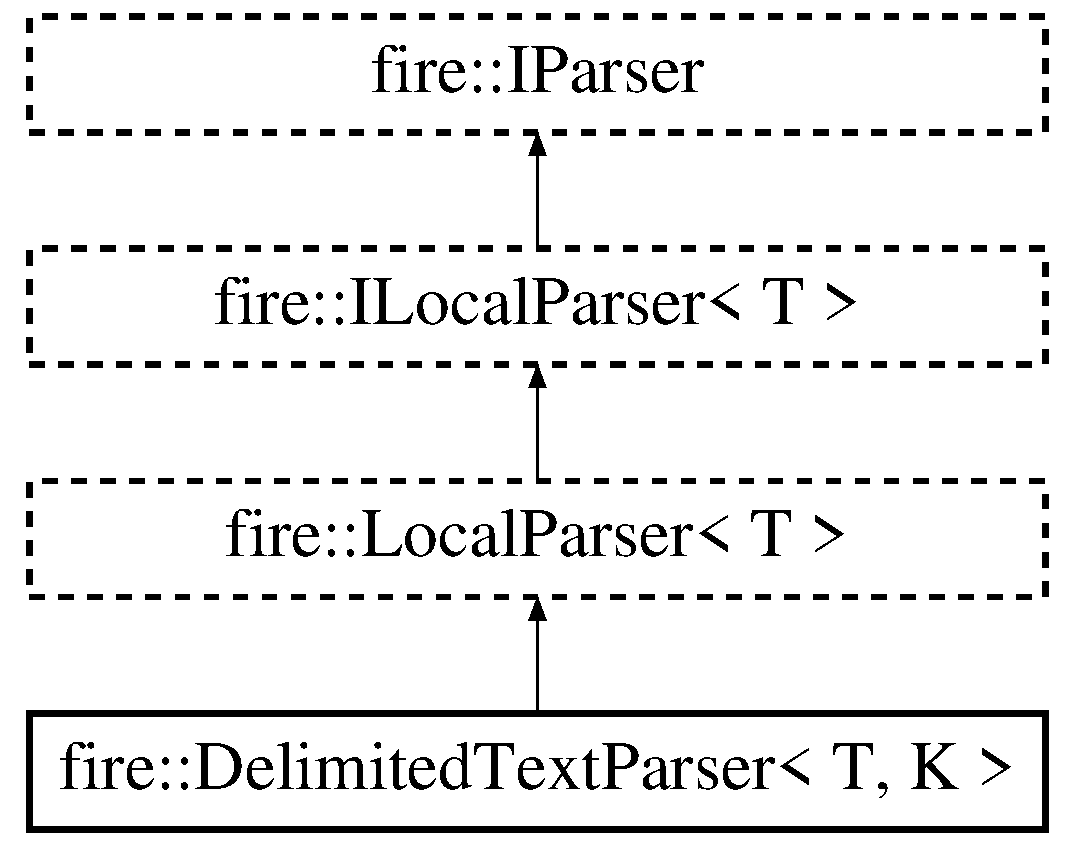
\includegraphics[height=4.000000cm]{a01271}
\end{center}
\end{figure}
\subsection*{Public Member Functions}
\begin{DoxyCompactItemize}
\item 
\mbox{\Hypertarget{a01271_aa1f041ebbf0bf72145e8bd20bf95f3f4}\label{a01271_aa1f041ebbf0bf72145e8bd20bf95f3f4}} 
{\bfseries Delimited\+Text\+Parser} (string delim, string comment)
\item 
virtual void \hyperlink{a01271_a686df5548771cae833d5e721442a821a}{parse} ()
\item 
{\footnotesize template$<$$>$ }\\void \hyperlink{a01271_a773fa7ed28cb9d8c384ad94bd81fc93f}{parse} ()
\end{DoxyCompactItemize}
\subsection*{Protected Attributes}
\begin{DoxyCompactItemize}
\item 
string \hyperlink{a01271_ac817fc333b53611a41f446977461bdbf}{delimiter}
\item 
string \hyperlink{a01271_acdd7b27b8109ed41e7d9bc5e6de72e93}{comment\+Char}
\end{DoxyCompactItemize}


\subsection{Detailed Description}
\subsubsection*{template$<$typename T, typename K$>$\newline
class fire\+::\+Delimited\+Text\+Parser$<$ T, K $>$}

This class implements \hyperlink{a01275}{I\+Local\+Parser} to provide a local, file-\/based, serially executed delimited text parser.

\hyperlink{a01275_a091d5cf56bf8f407854ef87f460b2958}{is\+File()} will return true if set\+Source(string) is used is\+Stream() will return true if set\+Source(istream) is used \hyperlink{a01275_a770acae6e216de3a9c7140a12de25d58}{is\+Local()} always returns true. \hyperlink{a01275_ad46898c516adcce38acbb4800dc9777b}{is\+Parallel()} always returns false.

Because delimited text is most often primitives, this class requires two template arguments. The first argument T is how the data should be returned and the second argument K is the root type of the delimited text, most likely a primitive. This would look something like


\begin{DoxyCode}
DelimitedTextParser<vector<vector<double>>,\textcolor{keywordtype}{double}>
\end{DoxyCode}


for a dense body of text like in a standard C\+SV file or D\+AT file where each column is composed of dense primitives.

The source may either be a file on the local filesystem or an input stream.

This is an extension of the parser interface that focuses on parsing delimited text. Delimited text is text with entries that are separated by a common pattern, such as a common or space.

The Comma-\/\+Separated Variables format is a delimited text format of the form

v1, v2, v3, v4

where each comma is the delimiter between the text values v1 through v4. A line of text with only spaces is also a delimited text format\+:

v1 v2 v3 v4

Delimited text parsers may assume that lines such as those above are terminated by ~\newline
. Like most other text formats, delimited text files may contain comments, which may be skipped by I\+Delimited\+Text\+Parsers. The characters that denote comments -\/ very commonly a \char`\"{}\#\char`\"{} or \char`\"{}//\char`\"{} -\/ may be passed to the constructor. 

\subsection{Member Function Documentation}
\mbox{\Hypertarget{a01271_a686df5548771cae833d5e721442a821a}\label{a01271_a686df5548771cae833d5e721442a821a}} 
\index{fire\+::\+Delimited\+Text\+Parser@{fire\+::\+Delimited\+Text\+Parser}!parse@{parse}}
\index{parse@{parse}!fire\+::\+Delimited\+Text\+Parser@{fire\+::\+Delimited\+Text\+Parser}}
\subsubsection{\texorpdfstring{parse()}{parse()}\hspace{0.1cm}{\footnotesize\ttfamily [1/2]}}
{\footnotesize\ttfamily template$<$typename T , typename K $>$ \\
virtual void \hyperlink{a01271}{fire\+::\+Delimited\+Text\+Parser}$<$ T, K $>$\+::parse (\begin{DoxyParamCaption}{ }\end{DoxyParamCaption})\hspace{0.3cm}{\ttfamily [inline]}, {\ttfamily [virtual]}}

This operation directs the parser to parse its source. 

Reimplemented from \hyperlink{a01291_abd8929aea06c2dda40256d2e58236650}{fire\+::\+Local\+Parser$<$ T $>$}.

\mbox{\Hypertarget{a01271_a773fa7ed28cb9d8c384ad94bd81fc93f}\label{a01271_a773fa7ed28cb9d8c384ad94bd81fc93f}} 
\index{fire\+::\+Delimited\+Text\+Parser@{fire\+::\+Delimited\+Text\+Parser}!parse@{parse}}
\index{parse@{parse}!fire\+::\+Delimited\+Text\+Parser@{fire\+::\+Delimited\+Text\+Parser}}
\subsubsection{\texorpdfstring{parse()}{parse()}\hspace{0.1cm}{\footnotesize\ttfamily [2/2]}}
{\footnotesize\ttfamily template$<$$>$ \\
void \hyperlink{a01271}{fire\+::\+Delimited\+Text\+Parser}$<$ vector$<$ vector$<$ double $>$ $>$, double $>$\+::parse (\begin{DoxyParamCaption}{ }\end{DoxyParamCaption})\hspace{0.3cm}{\ttfamily [virtual]}}

This specialization is for dense data of primitive type double. 

Reimplemented from \hyperlink{a01291_abd8929aea06c2dda40256d2e58236650}{fire\+::\+Local\+Parser$<$ T $>$}.



\subsection{Member Data Documentation}
\mbox{\Hypertarget{a01271_acdd7b27b8109ed41e7d9bc5e6de72e93}\label{a01271_acdd7b27b8109ed41e7d9bc5e6de72e93}} 
\index{fire\+::\+Delimited\+Text\+Parser@{fire\+::\+Delimited\+Text\+Parser}!comment\+Char@{comment\+Char}}
\index{comment\+Char@{comment\+Char}!fire\+::\+Delimited\+Text\+Parser@{fire\+::\+Delimited\+Text\+Parser}}
\subsubsection{\texorpdfstring{comment\+Char}{commentChar}}
{\footnotesize\ttfamily template$<$typename T , typename K $>$ \\
string \hyperlink{a01271}{fire\+::\+Delimited\+Text\+Parser}$<$ T, K $>$\+::comment\+Char\hspace{0.3cm}{\ttfamily [protected]}}

The character that represents a comment and should be skipped. \mbox{\Hypertarget{a01271_ac817fc333b53611a41f446977461bdbf}\label{a01271_ac817fc333b53611a41f446977461bdbf}} 
\index{fire\+::\+Delimited\+Text\+Parser@{fire\+::\+Delimited\+Text\+Parser}!delimiter@{delimiter}}
\index{delimiter@{delimiter}!fire\+::\+Delimited\+Text\+Parser@{fire\+::\+Delimited\+Text\+Parser}}
\subsubsection{\texorpdfstring{delimiter}{delimiter}}
{\footnotesize\ttfamily template$<$typename T , typename K $>$ \\
string \hyperlink{a01271}{fire\+::\+Delimited\+Text\+Parser}$<$ T, K $>$\+::delimiter\hspace{0.3cm}{\ttfamily [protected]}}

The delimiter used when parsing the file. 

The documentation for this class was generated from the following file\+:\begin{DoxyCompactItemize}
\item 
Delimited\+Text\+Parser.\+h\end{DoxyCompactItemize}

\hypertarget{a01143}{}\section{xacc\+:\+:Algorithm\+Generator Class Reference}
\label{a01143}\index{xacc\+::\+Algorithm\+Generator@{xacc\+::\+Algorithm\+Generator}}


{\ttfamily \#include $<$Algorithm\+Generator.\+hpp$>$}

Inheritance diagram for xacc\+:\+:Algorithm\+Generator\+:\begin{figure}[H]
\begin{center}
\leavevmode
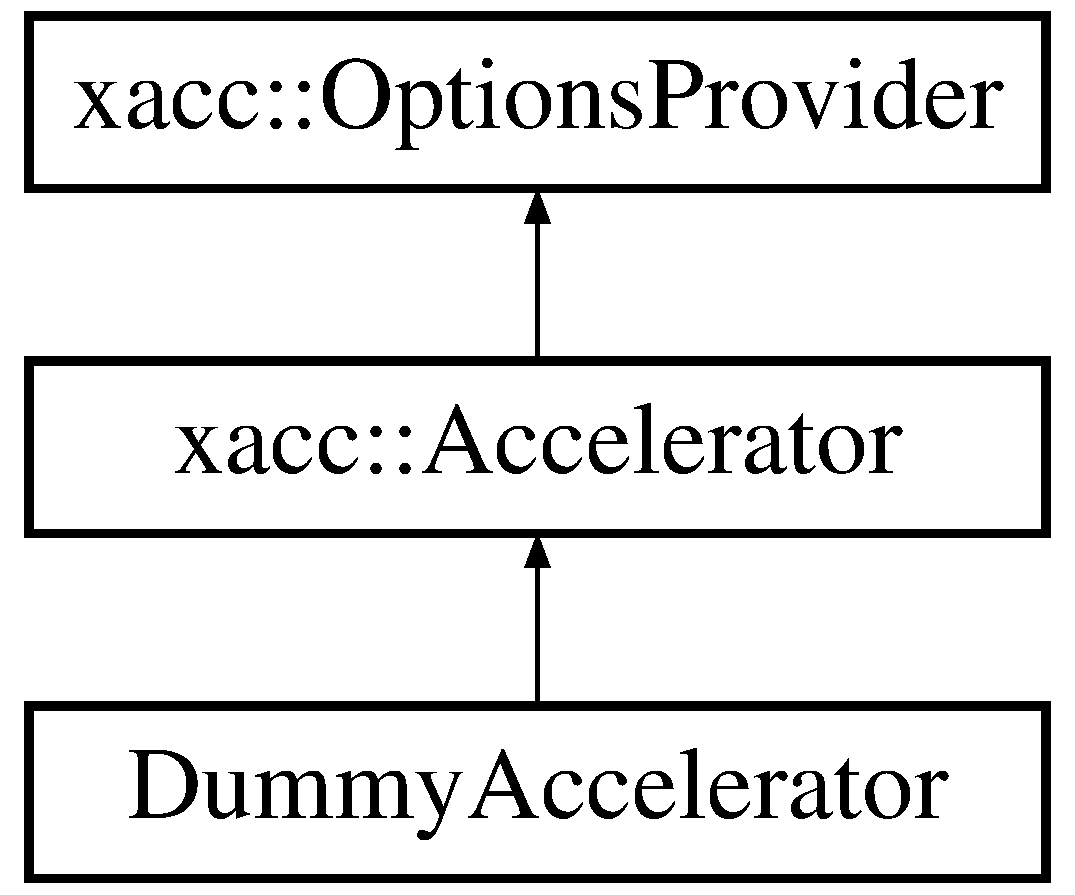
\includegraphics[height=2.000000cm]{a01143}
\end{center}
\end{figure}
\subsection*{Public Member Functions}
\begin{DoxyCompactItemize}
\item 
virtual std\+::shared\+\_\+ptr$<$ \hyperlink{a01151}{Function} $>$ \hyperlink{a01143_a73023c06f0f0c62ad56ab4187b18b096}{generate\+Algorithm} (std\+::vector$<$ int $>$ bits)=0
\item 
virtual \hyperlink{a01143_a096f66aa8d65f5aa3276915768159579}{$\sim$\+Algorithm\+Generator} ()
\end{DoxyCompactItemize}


\subsection{Detailed Description}
The \hyperlink{a01143}{Algorithm\+Generator} interface provides a mechanism for generating algorithms modeled as an X\+A\+CC \hyperlink{a01151}{Function} instance.

\begin{DoxyAuthor}{Author}
Alex Mc\+Caskey 
\end{DoxyAuthor}


\subsection{Constructor \& Destructor Documentation}
\mbox{\Hypertarget{a01143_a096f66aa8d65f5aa3276915768159579}\label{a01143_a096f66aa8d65f5aa3276915768159579}} 
\index{xacc\+::\+Algorithm\+Generator@{xacc\+::\+Algorithm\+Generator}!````~Algorithm\+Generator@{$\sim$\+Algorithm\+Generator}}
\index{````~Algorithm\+Generator@{$\sim$\+Algorithm\+Generator}!xacc\+::\+Algorithm\+Generator@{xacc\+::\+Algorithm\+Generator}}
\subsubsection{\texorpdfstring{$\sim$\+Algorithm\+Generator()}{~AlgorithmGenerator()}}
{\footnotesize\ttfamily virtual xacc\+::\+Algorithm\+Generator\+::$\sim$\+Algorithm\+Generator (\begin{DoxyParamCaption}{ }\end{DoxyParamCaption})\hspace{0.3cm}{\ttfamily [inline]}, {\ttfamily [virtual]}}

The destructor 

\subsection{Member Function Documentation}
\mbox{\Hypertarget{a01143_a73023c06f0f0c62ad56ab4187b18b096}\label{a01143_a73023c06f0f0c62ad56ab4187b18b096}} 
\index{xacc\+::\+Algorithm\+Generator@{xacc\+::\+Algorithm\+Generator}!generate\+Algorithm@{generate\+Algorithm}}
\index{generate\+Algorithm@{generate\+Algorithm}!xacc\+::\+Algorithm\+Generator@{xacc\+::\+Algorithm\+Generator}}
\subsubsection{\texorpdfstring{generate\+Algorithm()}{generateAlgorithm()}}
{\footnotesize\ttfamily virtual std\+::shared\+\_\+ptr$<$\hyperlink{a01151}{Function}$>$ xacc\+::\+Algorithm\+Generator\+::generate\+Algorithm (\begin{DoxyParamCaption}\item[{std\+::vector$<$ int $>$}]{bits }\end{DoxyParamCaption})\hspace{0.3cm}{\ttfamily [pure virtual]}}

Implementations of this method generate a \hyperlink{a01151}{Function} \hyperlink{a01175}{IR} instance corresponding to the implementation\textquotesingle{}s modeled algorithm. The algorithm is specified to operate over the provided bits.


\begin{DoxyParams}{Parameters}
{\em bits} & The bits this algorithm operates on \\
\hline
\end{DoxyParams}
\begin{DoxyReturn}{Returns}
function The algorithm represented as an \hyperlink{a01175}{IR} \hyperlink{a01151}{Function} 
\end{DoxyReturn}


Implemented in \hyperlink{a01007_ac093c288bc9fc069464fc3fd2cc0ac21}{xacc\+::quantum\+::\+Q\+FT}, and \hyperlink{a01003_af42e466bf02dbd60670d20aa55cfb08d}{xacc\+::quantum\+::\+Inverse\+Q\+FT}.



The documentation for this class was generated from the following file\+:\begin{DoxyCompactItemize}
\item 
Algorithm\+Generator.\+hpp\end{DoxyCompactItemize}

\hypertarget{a01139}{}\section{Dummy\+Compiler Class Reference}
\label{a01139}\index{Dummy\+Compiler@{Dummy\+Compiler}}
Inheritance diagram for Dummy\+Compiler\+:\begin{figure}[H]
\begin{center}
\leavevmode
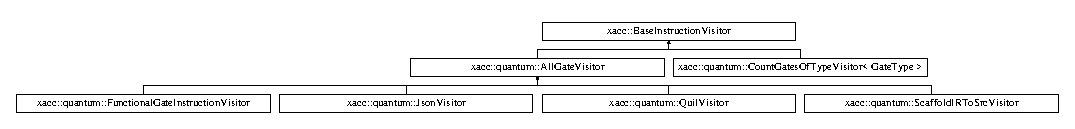
\includegraphics[height=3.000000cm]{a01139}
\end{center}
\end{figure}
\subsection*{Public Member Functions}
\begin{DoxyCompactItemize}
\item 
virtual std\+::shared\+\_\+ptr$<$ \hyperlink{a01499}{IR} $>$ \hyperlink{a01139_a9eaa6e6a4ff3645915d166a325bfde8d}{compile} (const std\+::string \&src, std\+::shared\+\_\+ptr$<$ \hyperlink{a01435}{Accelerator} $>$ acc)
\item 
virtual std\+::shared\+\_\+ptr$<$ \hyperlink{a01499}{IR} $>$ \hyperlink{a01139_a2f9bb3d30bb11f12b530854a11c8fb25}{compile} (const std\+::string \&src)
\item 
virtual const std\+::string \hyperlink{a01139_a606c27150c8d374242b8824e45b1e0c1}{translate} (const std\+::string \&buffer\+Variable, std\+::shared\+\_\+ptr$<$ \hyperlink{a01475}{Function} $>$ function)
\item 
virtual const std\+::string \hyperlink{a01139_a76460cb78671dc2cf42f2bebf8fb80c7}{get\+Name} ()
\end{DoxyCompactItemize}
\subsection*{Additional Inherited Members}


\subsection{Member Function Documentation}
\mbox{\Hypertarget{a01139_a9eaa6e6a4ff3645915d166a325bfde8d}\label{a01139_a9eaa6e6a4ff3645915d166a325bfde8d}} 
\index{Dummy\+Compiler@{Dummy\+Compiler}!compile@{compile}}
\index{compile@{compile}!Dummy\+Compiler@{Dummy\+Compiler}}
\subsubsection{\texorpdfstring{compile()}{compile()}\hspace{0.1cm}{\footnotesize\ttfamily [1/2]}}
{\footnotesize\ttfamily virtual std\+::shared\+\_\+ptr$<$\hyperlink{a01499}{IR}$>$ Dummy\+Compiler\+::compile (\begin{DoxyParamCaption}\item[{const std\+::string \&}]{src,  }\item[{std\+::shared\+\_\+ptr$<$ \hyperlink{a01435}{Accelerator} $>$}]{acc }\end{DoxyParamCaption})\hspace{0.3cm}{\ttfamily [inline]}, {\ttfamily [virtual]}}

This method is to be implemented by derived Compilers and is in charge of executing the compilation mechanism on the provided source string. Implementations also are given access to the Accelerator that this source code is intended for.


\begin{DoxyParams}{Parameters}
{\em src} & The kernel source string. \\
\hline
{\em acc} & The Accelerator this code will be executed on \\
\hline
\end{DoxyParams}
\begin{DoxyReturn}{Returns}
ir Intermediate representation for provided source kernel code. 
\end{DoxyReturn}


Implements \hyperlink{a01451_a546a40c95bb93af6a0c0ac48dbeaffc8}{xacc\+::\+Compiler}.

\mbox{\Hypertarget{a01139_a2f9bb3d30bb11f12b530854a11c8fb25}\label{a01139_a2f9bb3d30bb11f12b530854a11c8fb25}} 
\index{Dummy\+Compiler@{Dummy\+Compiler}!compile@{compile}}
\index{compile@{compile}!Dummy\+Compiler@{Dummy\+Compiler}}
\subsubsection{\texorpdfstring{compile()}{compile()}\hspace{0.1cm}{\footnotesize\ttfamily [2/2]}}
{\footnotesize\ttfamily virtual std\+::shared\+\_\+ptr$<$\hyperlink{a01499}{IR}$>$ Dummy\+Compiler\+::compile (\begin{DoxyParamCaption}\item[{const std\+::string \&}]{src }\end{DoxyParamCaption})\hspace{0.3cm}{\ttfamily [inline]}, {\ttfamily [virtual]}}

This method is to be implemented by derived Compilers and is in charge of executing the compilation mechanism on the provided source string. 
\begin{DoxyParams}{Parameters}
{\em src} & \\
\hline
\end{DoxyParams}
\begin{DoxyReturn}{Returns}

\end{DoxyReturn}


Implements \hyperlink{a01451_a9092f5f779b570c91569b59621280c04}{xacc\+::\+Compiler}.

\mbox{\Hypertarget{a01139_a76460cb78671dc2cf42f2bebf8fb80c7}\label{a01139_a76460cb78671dc2cf42f2bebf8fb80c7}} 
\index{Dummy\+Compiler@{Dummy\+Compiler}!get\+Name@{get\+Name}}
\index{get\+Name@{get\+Name}!Dummy\+Compiler@{Dummy\+Compiler}}
\subsubsection{\texorpdfstring{get\+Name()}{getName()}}
{\footnotesize\ttfamily virtual const std\+::string Dummy\+Compiler\+::get\+Name (\begin{DoxyParamCaption}{ }\end{DoxyParamCaption})\hspace{0.3cm}{\ttfamily [inline]}, {\ttfamily [virtual]}}

Return the name of this Compiler \begin{DoxyReturn}{Returns}
name Compiler name 
\end{DoxyReturn}


Implements \hyperlink{a01451_a87fca9100e6462122f5b687c3a0fb3fb}{xacc\+::\+Compiler}.

\mbox{\Hypertarget{a01139_a606c27150c8d374242b8824e45b1e0c1}\label{a01139_a606c27150c8d374242b8824e45b1e0c1}} 
\index{Dummy\+Compiler@{Dummy\+Compiler}!translate@{translate}}
\index{translate@{translate}!Dummy\+Compiler@{Dummy\+Compiler}}
\subsubsection{\texorpdfstring{translate()}{translate()}}
{\footnotesize\ttfamily virtual const std\+::string Dummy\+Compiler\+::translate (\begin{DoxyParamCaption}\item[{const std\+::string \&}]{buffer\+Variable,  }\item[{std\+::shared\+\_\+ptr$<$ \hyperlink{a01475}{Function} $>$}]{function }\end{DoxyParamCaption})\hspace{0.3cm}{\ttfamily [inline]}, {\ttfamily [virtual]}}

This method is to be implemented by derived Compilers and is in charge of taking the provided Function IR and converting it to source code in this Compiler\textquotesingle{}s language.


\begin{DoxyParams}{Parameters}
{\em function} & The X\+A\+CC IR Function to translate \\
\hline
\end{DoxyParams}
\begin{DoxyReturn}{Returns}
src The source code as a string 
\end{DoxyReturn}


Implements \hyperlink{a01451_aeedbe58a33fed29e4d7694ae743e25e7}{xacc\+::\+Compiler}.



The documentation for this class was generated from the following file\+:\begin{DoxyCompactItemize}
\item 
Kernel\+Replacement\+Preprocessor\+Tester.\+cpp\end{DoxyCompactItemize}

\hypertarget{a01115}{}\section{xacc\+:\+:Register\+Preprocessor$<$ T $>$ Class Template Reference}
\label{a01115}\index{xacc\+::\+Register\+Preprocessor$<$ T $>$@{xacc\+::\+Register\+Preprocessor$<$ T $>$}}


{\ttfamily \#include $<$Preprocessor.\+hpp$>$}

\subsection*{Public Member Functions}
\begin{DoxyCompactItemize}
\item 
\mbox{\Hypertarget{a01115_a360d5ffa16ef3a96c3bc61fa897ffe3c}\label{a01115_a360d5ffa16ef3a96c3bc61fa897ffe3c}} 
{\bfseries Register\+Preprocessor} (const std\+::string \&name)
\end{DoxyCompactItemize}


\subsection{Detailed Description}
\subsubsection*{template$<$typename T$>$\newline
class xacc\+::\+Register\+Preprocessor$<$ T $>$}

\hyperlink{a01115}{Register\+Preprocessor} is a convenience class for registering custom derived \hyperlink{a01111}{Preprocessor} classes.

Creators of \hyperlink{a01111}{Preprocessor} subclasses create an instance of this class with their \hyperlink{a01111}{Preprocessor} subclass as the template parameter to register their \hyperlink{a01111}{Preprocessor} with X\+A\+CC. This instance must be created in the C\+PP implementation file for the \hyperlink{a01111}{Preprocessor} and at global scope. 

The documentation for this class was generated from the following file\+:\begin{DoxyCompactItemize}
\item 
Preprocessor.\+hpp\end{DoxyCompactItemize}

\hypertarget{a01131}{}\section{xacc\+:\+:Instruction Class Reference}
\label{a01131}\index{xacc\+::\+Instruction@{xacc\+::\+Instruction}}


{\ttfamily \#include $<$Instruction.\+hpp$>$}

Inheritance diagram for xacc\+:\+:Instruction\+:\begin{figure}[H]
\begin{center}
\leavevmode
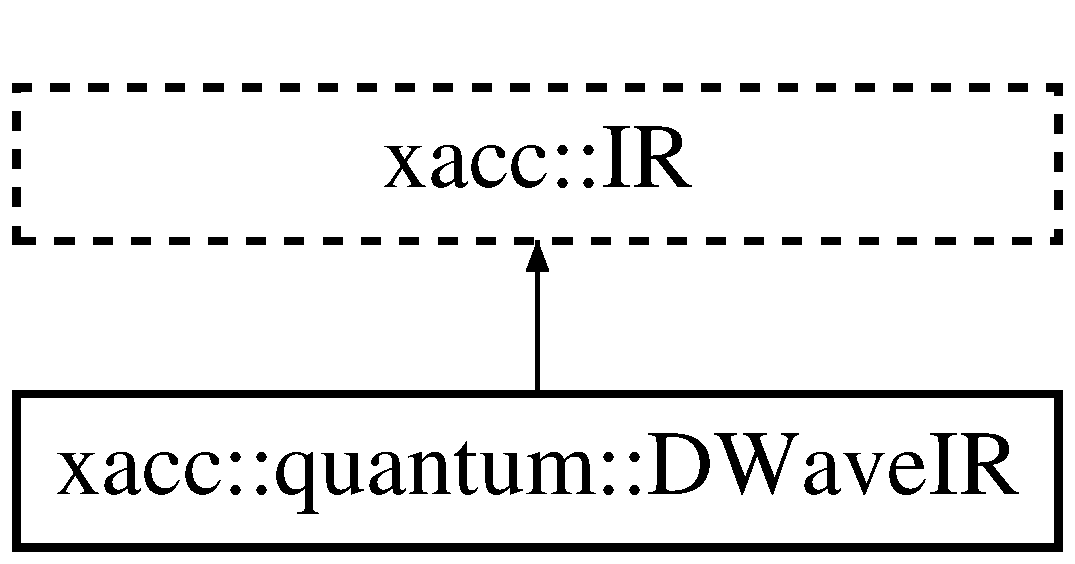
\includegraphics[height=12.000000cm]{a01131}
\end{center}
\end{figure}
\subsection*{Public Member Functions}
\begin{DoxyCompactItemize}
\item 
virtual const std\+::string \hyperlink{a01131_ac7ff23f693e2276edbf3fdac5452792c}{get\+Name} ()=0
\item 
virtual const std\+::string \hyperlink{a01131_ae94c2d089908294c1d410b14c96817ae}{to\+String} (const std\+::string \&buffer\+Var\+Name)=0
\item 
virtual const std\+::vector$<$ int $>$ \hyperlink{a01131_a819f32e94c3e1c9e69a0061aaf8d86dc}{bits} ()=0
\item 
virtual Instruction\+Parameter \hyperlink{a01131_aa0d9de97a4833a042379647f83c33ab6}{get\+Parameter} (const int idx)=0
\item 
virtual std\+::vector$<$ Instruction\+Parameter $>$ \hyperlink{a01131_aeb67c67713896e8f27a5c7dd531f3340}{get\+Parameters} ()=0
\item 
virtual void \hyperlink{a01131_a407a0ac662fa0b1ec3e301e8ff9bade7}{set\+Parameter} (const int idx, Instruction\+Parameter \&isnt)=0
\item 
virtual const int \hyperlink{a01131_ad54585d13c04ffd20296fff7ab8107ff}{n\+Parameters} ()=0
\item 
virtual bool \hyperlink{a01131_a7b24d8ae485369fc2b2df7a3224a5e26}{is\+Parameterized} ()
\item 
virtual bool \hyperlink{a01131_a4383f1036d0fcfe890ab9c613dbd5f38}{is\+Composite} ()
\item 
virtual bool \hyperlink{a01131_ad02a1cf7220577124720b7a51424cea7}{is\+Enabled} ()
\item 
virtual void \hyperlink{a01131_a6e528da15e05a94cc1d7db268c483271}{disable} ()
\item 
virtual void \hyperlink{a01131_a0b4f2e5a591af28342a3c08e4305e24f}{enable} ()
\item 
virtual \hyperlink{a01131_ae22c935e8113bce63d1d0e214cda4d61}{$\sim$\+Instruction} ()
\end{DoxyCompactItemize}
\subsection*{Additional Inherited Members}


\subsection{Detailed Description}
The \hyperlink{a01131}{Instruction} interface is the base of all X\+A\+CC Intermediate Representation Instructions for post-\/\+Moore\textquotesingle{}s law accelerated computing. The \hyperlink{a01131}{Instruction}, at its core, provides an \hyperlink{a01131}{Instruction} name and a set of next-\/gen bits that the \hyperlink{a01131}{Instruction} operates on. Instructions can also be enabled or disabled. Instructions implement \hyperlink{a01147}{Base\+Instruction\+Visitable} to enable visitor pattern functionality across all \hyperlink{a01131}{Instruction} subclasses.

\hyperlink{a01131}{Instruction} can also expose 0 to N Instruction\+Parameters. Instruction\+Parameters can be an int, double, float, or string. 

\subsection{Constructor \& Destructor Documentation}
\mbox{\Hypertarget{a01131_ae22c935e8113bce63d1d0e214cda4d61}\label{a01131_ae22c935e8113bce63d1d0e214cda4d61}} 
\index{xacc\+::\+Instruction@{xacc\+::\+Instruction}!````~Instruction@{$\sim$\+Instruction}}
\index{````~Instruction@{$\sim$\+Instruction}!xacc\+::\+Instruction@{xacc\+::\+Instruction}}
\subsubsection{\texorpdfstring{$\sim$\+Instruction()}{~Instruction()}}
{\footnotesize\ttfamily virtual xacc\+::\+Instruction\+::$\sim$\+Instruction (\begin{DoxyParamCaption}{ }\end{DoxyParamCaption})\hspace{0.3cm}{\ttfamily [inline]}, {\ttfamily [virtual]}}

The destructor 

\subsection{Member Function Documentation}
\mbox{\Hypertarget{a01131_a819f32e94c3e1c9e69a0061aaf8d86dc}\label{a01131_a819f32e94c3e1c9e69a0061aaf8d86dc}} 
\index{xacc\+::\+Instruction@{xacc\+::\+Instruction}!bits@{bits}}
\index{bits@{bits}!xacc\+::\+Instruction@{xacc\+::\+Instruction}}
\subsubsection{\texorpdfstring{bits()}{bits()}}
{\footnotesize\ttfamily virtual const std\+::vector$<$int$>$ xacc\+::\+Instruction\+::bits (\begin{DoxyParamCaption}{ }\end{DoxyParamCaption})\hspace{0.3cm}{\ttfamily [pure virtual]}}

Return the indices of the bits that this \hyperlink{a01131}{Instruction} operates on.

\begin{DoxyReturn}{Returns}
bits The bits this \hyperlink{a01131}{Instruction} operates on. 
\end{DoxyReturn}


Implemented in \hyperlink{a00987_aba03de68b76a9e120705c3c389c714a1}{xacc\+::quantum\+::\+Gate\+Function}, and \hyperlink{a00991_ad32ad03dfc516e00093030e60178003d}{xacc\+::quantum\+::\+Gate\+Instruction}.

\mbox{\Hypertarget{a01131_a6e528da15e05a94cc1d7db268c483271}\label{a01131_a6e528da15e05a94cc1d7db268c483271}} 
\index{xacc\+::\+Instruction@{xacc\+::\+Instruction}!disable@{disable}}
\index{disable@{disable}!xacc\+::\+Instruction@{xacc\+::\+Instruction}}
\subsubsection{\texorpdfstring{disable()}{disable()}}
{\footnotesize\ttfamily virtual void xacc\+::\+Instruction\+::disable (\begin{DoxyParamCaption}{ }\end{DoxyParamCaption})\hspace{0.3cm}{\ttfamily [inline]}, {\ttfamily [virtual]}}

Disable this \hyperlink{a01131}{Instruction} 

Reimplemented in \hyperlink{a00991_a63ce138dd71fb43d303f5600fefb7215}{xacc\+::quantum\+::\+Gate\+Instruction}.

\mbox{\Hypertarget{a01131_a0b4f2e5a591af28342a3c08e4305e24f}\label{a01131_a0b4f2e5a591af28342a3c08e4305e24f}} 
\index{xacc\+::\+Instruction@{xacc\+::\+Instruction}!enable@{enable}}
\index{enable@{enable}!xacc\+::\+Instruction@{xacc\+::\+Instruction}}
\subsubsection{\texorpdfstring{enable()}{enable()}}
{\footnotesize\ttfamily virtual void xacc\+::\+Instruction\+::enable (\begin{DoxyParamCaption}{ }\end{DoxyParamCaption})\hspace{0.3cm}{\ttfamily [inline]}, {\ttfamily [virtual]}}

Enable this \hyperlink{a01131}{Instruction}. 

Reimplemented in \hyperlink{a00991_a7a80474b7fd465271b3313432db2e608}{xacc\+::quantum\+::\+Gate\+Instruction}.

\mbox{\Hypertarget{a01131_ac7ff23f693e2276edbf3fdac5452792c}\label{a01131_ac7ff23f693e2276edbf3fdac5452792c}} 
\index{xacc\+::\+Instruction@{xacc\+::\+Instruction}!get\+Name@{get\+Name}}
\index{get\+Name@{get\+Name}!xacc\+::\+Instruction@{xacc\+::\+Instruction}}
\subsubsection{\texorpdfstring{get\+Name()}{getName()}}
{\footnotesize\ttfamily virtual const std\+::string xacc\+::\+Instruction\+::get\+Name (\begin{DoxyParamCaption}{ }\end{DoxyParamCaption})\hspace{0.3cm}{\ttfamily [pure virtual]}}

Return the name of this \hyperlink{a01131}{Instruction}

\begin{DoxyReturn}{Returns}
name The name of this \hyperlink{a01131}{Instruction} 
\end{DoxyReturn}


Implemented in \hyperlink{a00987_af42efb6191267164717d53c469e15d3a}{xacc\+::quantum\+::\+Gate\+Function}, and \hyperlink{a00991_a0db03b9e46eeba1134f0ca2b83ccc842}{xacc\+::quantum\+::\+Gate\+Instruction}.

\mbox{\Hypertarget{a01131_aa0d9de97a4833a042379647f83c33ab6}\label{a01131_aa0d9de97a4833a042379647f83c33ab6}} 
\index{xacc\+::\+Instruction@{xacc\+::\+Instruction}!get\+Parameter@{get\+Parameter}}
\index{get\+Parameter@{get\+Parameter}!xacc\+::\+Instruction@{xacc\+::\+Instruction}}
\subsubsection{\texorpdfstring{get\+Parameter()}{getParameter()}}
{\footnotesize\ttfamily virtual Instruction\+Parameter xacc\+::\+Instruction\+::get\+Parameter (\begin{DoxyParamCaption}\item[{const int}]{idx }\end{DoxyParamCaption})\hspace{0.3cm}{\ttfamily [pure virtual]}}

Return this \hyperlink{a01131}{Instruction}\textquotesingle{}s parameter at the given index.


\begin{DoxyParams}{Parameters}
{\em idx} & The index of the parameter. \\
\hline
\end{DoxyParams}
\begin{DoxyReturn}{Returns}
param The Instruction\+Parameter at the given index. 
\end{DoxyReturn}


Implemented in \hyperlink{a00987_a5991903323e412777bedc4f0c862eb63}{xacc\+::quantum\+::\+Gate\+Function}, and \hyperlink{a00991_addd6185279fe99fbdc3d4efd96e42162}{xacc\+::quantum\+::\+Gate\+Instruction}.

\mbox{\Hypertarget{a01131_aeb67c67713896e8f27a5c7dd531f3340}\label{a01131_aeb67c67713896e8f27a5c7dd531f3340}} 
\index{xacc\+::\+Instruction@{xacc\+::\+Instruction}!get\+Parameters@{get\+Parameters}}
\index{get\+Parameters@{get\+Parameters}!xacc\+::\+Instruction@{xacc\+::\+Instruction}}
\subsubsection{\texorpdfstring{get\+Parameters()}{getParameters()}}
{\footnotesize\ttfamily virtual std\+::vector$<$Instruction\+Parameter$>$ xacc\+::\+Instruction\+::get\+Parameters (\begin{DoxyParamCaption}{ }\end{DoxyParamCaption})\hspace{0.3cm}{\ttfamily [pure virtual]}}

Return all of this \hyperlink{a01131}{Instruction}\textquotesingle{}s parameters.

\begin{DoxyReturn}{Returns}
params This instructions parameters. 
\end{DoxyReturn}


Implemented in \hyperlink{a00987_af7aabfe699a4dced576ff7fafff969d5}{xacc\+::quantum\+::\+Gate\+Function}, and \hyperlink{a00991_a8584444f9577283f6844ab32bdc4db72}{xacc\+::quantum\+::\+Gate\+Instruction}.

\mbox{\Hypertarget{a01131_a4383f1036d0fcfe890ab9c613dbd5f38}\label{a01131_a4383f1036d0fcfe890ab9c613dbd5f38}} 
\index{xacc\+::\+Instruction@{xacc\+::\+Instruction}!is\+Composite@{is\+Composite}}
\index{is\+Composite@{is\+Composite}!xacc\+::\+Instruction@{xacc\+::\+Instruction}}
\subsubsection{\texorpdfstring{is\+Composite()}{isComposite()}}
{\footnotesize\ttfamily virtual bool xacc\+::\+Instruction\+::is\+Composite (\begin{DoxyParamCaption}{ }\end{DoxyParamCaption})\hspace{0.3cm}{\ttfamily [inline]}, {\ttfamily [virtual]}}

Returns true if this \hyperlink{a01131}{Instruction} is composite, ie, contains other Instructions.

\begin{DoxyReturn}{Returns}
is\+Composite True if this is a composite \hyperlink{a01131}{Instruction} 
\end{DoxyReturn}


Reimplemented in \hyperlink{a01127_aa75500c657b5c3e0e36213e1506aad97}{xacc\+::\+Function}.

\mbox{\Hypertarget{a01131_ad02a1cf7220577124720b7a51424cea7}\label{a01131_ad02a1cf7220577124720b7a51424cea7}} 
\index{xacc\+::\+Instruction@{xacc\+::\+Instruction}!is\+Enabled@{is\+Enabled}}
\index{is\+Enabled@{is\+Enabled}!xacc\+::\+Instruction@{xacc\+::\+Instruction}}
\subsubsection{\texorpdfstring{is\+Enabled()}{isEnabled()}}
{\footnotesize\ttfamily virtual bool xacc\+::\+Instruction\+::is\+Enabled (\begin{DoxyParamCaption}{ }\end{DoxyParamCaption})\hspace{0.3cm}{\ttfamily [inline]}, {\ttfamily [virtual]}}

Returns true if this \hyperlink{a01131}{Instruction} is enabled

\begin{DoxyReturn}{Returns}
enabled True if this \hyperlink{a01131}{Instruction} is enabled. 
\end{DoxyReturn}


Reimplemented in \hyperlink{a00991_a0a821be322b0c848b01c55f91fc8f484}{xacc\+::quantum\+::\+Gate\+Instruction}.

\mbox{\Hypertarget{a01131_a7b24d8ae485369fc2b2df7a3224a5e26}\label{a01131_a7b24d8ae485369fc2b2df7a3224a5e26}} 
\index{xacc\+::\+Instruction@{xacc\+::\+Instruction}!is\+Parameterized@{is\+Parameterized}}
\index{is\+Parameterized@{is\+Parameterized}!xacc\+::\+Instruction@{xacc\+::\+Instruction}}
\subsubsection{\texorpdfstring{is\+Parameterized()}{isParameterized()}}
{\footnotesize\ttfamily virtual bool xacc\+::\+Instruction\+::is\+Parameterized (\begin{DoxyParamCaption}{ }\end{DoxyParamCaption})\hspace{0.3cm}{\ttfamily [inline]}, {\ttfamily [virtual]}}

Return true if this \hyperlink{a01131}{Instruction} is parameterized.

\begin{DoxyReturn}{Returns}
parameterized True if this \hyperlink{a01131}{Instruction} has parameters. 
\end{DoxyReturn}


Reimplemented in \hyperlink{a00987_afad47903e0ed55ddbfa827ef8408a94b}{xacc\+::quantum\+::\+Gate\+Function}, and \hyperlink{a00991_afe7aeeb398262931e156bcb3950f8188}{xacc\+::quantum\+::\+Gate\+Instruction}.

\mbox{\Hypertarget{a01131_ad54585d13c04ffd20296fff7ab8107ff}\label{a01131_ad54585d13c04ffd20296fff7ab8107ff}} 
\index{xacc\+::\+Instruction@{xacc\+::\+Instruction}!n\+Parameters@{n\+Parameters}}
\index{n\+Parameters@{n\+Parameters}!xacc\+::\+Instruction@{xacc\+::\+Instruction}}
\subsubsection{\texorpdfstring{n\+Parameters()}{nParameters()}}
{\footnotesize\ttfamily virtual const int xacc\+::\+Instruction\+::n\+Parameters (\begin{DoxyParamCaption}{ }\end{DoxyParamCaption})\hspace{0.3cm}{\ttfamily [pure virtual]}}

Return the number of Instruction\+Parameters this \hyperlink{a01131}{Instruction} contains.

\begin{DoxyReturn}{Returns}
n\+Insts The number of instructions. 
\end{DoxyReturn}


Implemented in \hyperlink{a00987_ad0bffcbc0884d81d6bdddf55385fc6c9}{xacc\+::quantum\+::\+Gate\+Function}, and \hyperlink{a00991_a3752912b2c402668ca4814e21d4bbd26}{xacc\+::quantum\+::\+Gate\+Instruction}.

\mbox{\Hypertarget{a01131_a407a0ac662fa0b1ec3e301e8ff9bade7}\label{a01131_a407a0ac662fa0b1ec3e301e8ff9bade7}} 
\index{xacc\+::\+Instruction@{xacc\+::\+Instruction}!set\+Parameter@{set\+Parameter}}
\index{set\+Parameter@{set\+Parameter}!xacc\+::\+Instruction@{xacc\+::\+Instruction}}
\subsubsection{\texorpdfstring{set\+Parameter()}{setParameter()}}
{\footnotesize\ttfamily virtual void xacc\+::\+Instruction\+::set\+Parameter (\begin{DoxyParamCaption}\item[{const int}]{idx,  }\item[{Instruction\+Parameter \&}]{isnt }\end{DoxyParamCaption})\hspace{0.3cm}{\ttfamily [pure virtual]}}

Set this \hyperlink{a01131}{Instruction}\textquotesingle{}s parameter at the given index.


\begin{DoxyParams}{Parameters}
{\em idx} & The index of the parameter \\
\hline
{\em inst} & The instruction. \\
\hline
\end{DoxyParams}


Implemented in \hyperlink{a00987_ab8d9789b46e92e27a9d7c9c5b7e3683c}{xacc\+::quantum\+::\+Gate\+Function}, and \hyperlink{a00991_afb8f7582d7520c77d61b9016753f5669}{xacc\+::quantum\+::\+Gate\+Instruction}.

\mbox{\Hypertarget{a01131_ae94c2d089908294c1d410b14c96817ae}\label{a01131_ae94c2d089908294c1d410b14c96817ae}} 
\index{xacc\+::\+Instruction@{xacc\+::\+Instruction}!to\+String@{to\+String}}
\index{to\+String@{to\+String}!xacc\+::\+Instruction@{xacc\+::\+Instruction}}
\subsubsection{\texorpdfstring{to\+String()}{toString()}}
{\footnotesize\ttfamily virtual const std\+::string xacc\+::\+Instruction\+::to\+String (\begin{DoxyParamCaption}\item[{const std\+::string \&}]{buffer\+Var\+Name }\end{DoxyParamCaption})\hspace{0.3cm}{\ttfamily [pure virtual]}}

Persist this \hyperlink{a01131}{Instruction} to an assembly-\/like string.


\begin{DoxyParams}{Parameters}
{\em buffer\+Var\+Name} & The name of the \hyperlink{a01099}{Accelerator\+Buffer} \\
\hline
\end{DoxyParams}
\begin{DoxyReturn}{Returns}
str The assembly-\/like string. 
\end{DoxyReturn}


Implemented in \hyperlink{a00987_aa1950776ae84bad2d0795a0441f910e7}{xacc\+::quantum\+::\+Gate\+Function}, \hyperlink{a00991_a089a5da67ff40ac1a6f56e64589822d9}{xacc\+::quantum\+::\+Gate\+Instruction}, \hyperlink{a01023_a1c51a5d68294dcb2ba1a9fbea63a730f}{xacc\+::quantum\+::\+Measure}, and \hyperlink{a01011_aca7a5f849fece6fc28a904efee9a3370}{xacc\+::quantum\+::\+Conditional\+Function}.



The documentation for this class was generated from the following file\+:\begin{DoxyCompactItemize}
\item 
Instruction.\+hpp\end{DoxyCompactItemize}

\hypertarget{a01119}{}\section{xacc\+:\+:Algorithm\+Generator Class Reference}
\label{a01119}\index{xacc\+::\+Algorithm\+Generator@{xacc\+::\+Algorithm\+Generator}}


{\ttfamily \#include $<$Algorithm\+Generator.\+hpp$>$}

Inheritance diagram for xacc\+:\+:Algorithm\+Generator\+:\begin{figure}[H]
\begin{center}
\leavevmode
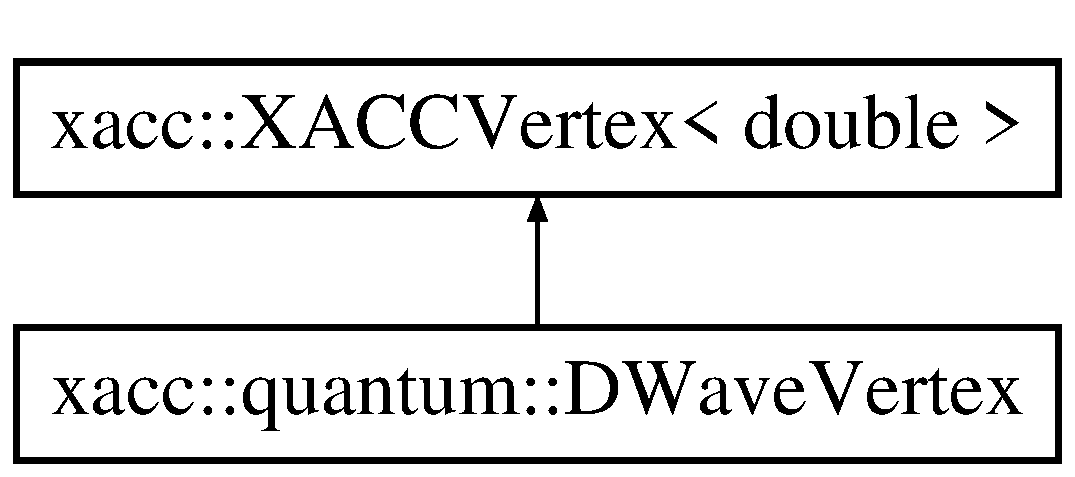
\includegraphics[height=2.000000cm]{a01119}
\end{center}
\end{figure}
\subsection*{Public Member Functions}
\begin{DoxyCompactItemize}
\item 
virtual std\+::shared\+\_\+ptr$<$ \hyperlink{a01127}{Function} $>$ \hyperlink{a01119_a73023c06f0f0c62ad56ab4187b18b096}{generate\+Algorithm} (std\+::vector$<$ int $>$ bits)=0
\item 
virtual \hyperlink{a01119_a096f66aa8d65f5aa3276915768159579}{$\sim$\+Algorithm\+Generator} ()
\end{DoxyCompactItemize}


\subsection{Detailed Description}
The \hyperlink{a01119}{Algorithm\+Generator} interface provides a mechanism for generating algorithms modeled as an X\+A\+CC \hyperlink{a01127}{Function} instance.

\begin{DoxyAuthor}{Author}
Alex Mc\+Caskey 
\end{DoxyAuthor}


\subsection{Constructor \& Destructor Documentation}
\mbox{\Hypertarget{a01119_a096f66aa8d65f5aa3276915768159579}\label{a01119_a096f66aa8d65f5aa3276915768159579}} 
\index{xacc\+::\+Algorithm\+Generator@{xacc\+::\+Algorithm\+Generator}!````~Algorithm\+Generator@{$\sim$\+Algorithm\+Generator}}
\index{````~Algorithm\+Generator@{$\sim$\+Algorithm\+Generator}!xacc\+::\+Algorithm\+Generator@{xacc\+::\+Algorithm\+Generator}}
\subsubsection{\texorpdfstring{$\sim$\+Algorithm\+Generator()}{~AlgorithmGenerator()}}
{\footnotesize\ttfamily virtual xacc\+::\+Algorithm\+Generator\+::$\sim$\+Algorithm\+Generator (\begin{DoxyParamCaption}{ }\end{DoxyParamCaption})\hspace{0.3cm}{\ttfamily [inline]}, {\ttfamily [virtual]}}

The destructor 

\subsection{Member Function Documentation}
\mbox{\Hypertarget{a01119_a73023c06f0f0c62ad56ab4187b18b096}\label{a01119_a73023c06f0f0c62ad56ab4187b18b096}} 
\index{xacc\+::\+Algorithm\+Generator@{xacc\+::\+Algorithm\+Generator}!generate\+Algorithm@{generate\+Algorithm}}
\index{generate\+Algorithm@{generate\+Algorithm}!xacc\+::\+Algorithm\+Generator@{xacc\+::\+Algorithm\+Generator}}
\subsubsection{\texorpdfstring{generate\+Algorithm()}{generateAlgorithm()}}
{\footnotesize\ttfamily virtual std\+::shared\+\_\+ptr$<$\hyperlink{a01127}{Function}$>$ xacc\+::\+Algorithm\+Generator\+::generate\+Algorithm (\begin{DoxyParamCaption}\item[{std\+::vector$<$ int $>$}]{bits }\end{DoxyParamCaption})\hspace{0.3cm}{\ttfamily [pure virtual]}}

Implementations of this method generate a \hyperlink{a01127}{Function} \hyperlink{a01151}{IR} instance corresponding to the implementation\textquotesingle{}s modeled algorithm. The algorithm is specified to operate over the provided bits.


\begin{DoxyParams}{Parameters}
{\em bits} & The bits this algorithm operates on \\
\hline
\end{DoxyParams}
\begin{DoxyReturn}{Returns}
function The algorithm represented as an \hyperlink{a01151}{IR} \hyperlink{a01127}{Function} 
\end{DoxyReturn}


Implemented in \hyperlink{a00983_ac093c288bc9fc069464fc3fd2cc0ac21}{xacc\+::quantum\+::\+Q\+FT}, and \hyperlink{a00979_af42e466bf02dbd60670d20aa55cfb08d}{xacc\+::quantum\+::\+Inverse\+Q\+FT}.



The documentation for this class was generated from the following file\+:\begin{DoxyCompactItemize}
\item 
Algorithm\+Generator.\+hpp\end{DoxyCompactItemize}

\hypertarget{a01343}{}\section{fire\+:\+:Eigen\+Provider Class Reference}
\label{a01343}\index{fire\+::\+Eigen\+Provider@{fire\+::\+Eigen\+Provider}}


{\ttfamily \#include $<$Eigen\+Tensor\+Provider.\+hpp$>$}

Inheritance diagram for fire\+:\+:Eigen\+Provider\+:\begin{figure}[H]
\begin{center}
\leavevmode
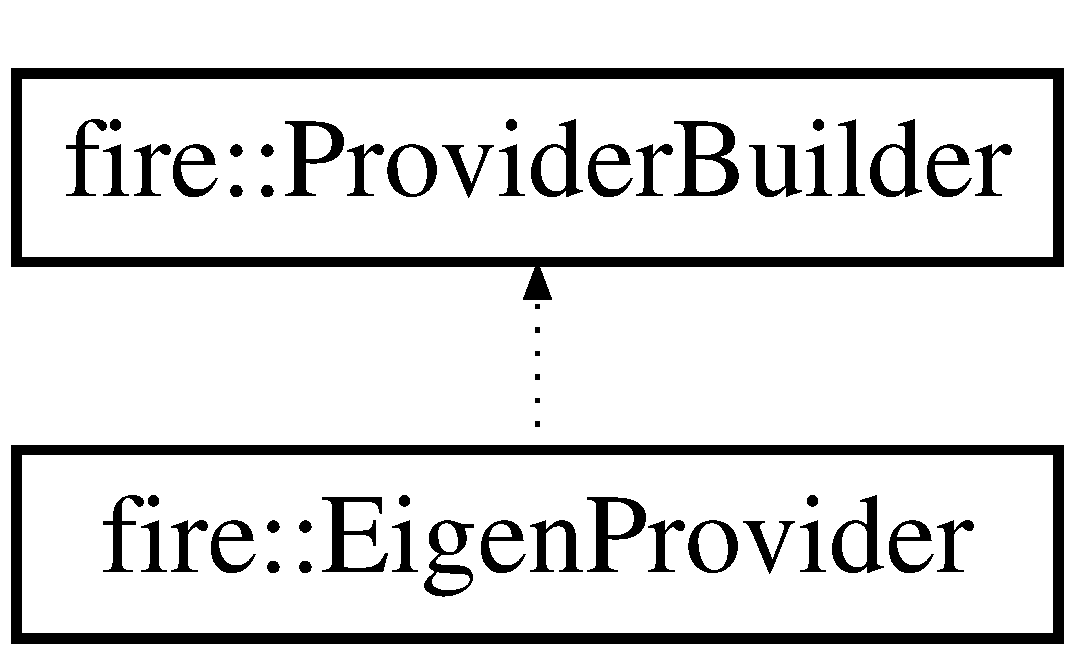
\includegraphics[height=2.000000cm]{a01343}
\end{center}
\end{figure}
\subsection*{Public Member Functions}
\begin{DoxyCompactItemize}
\item 
\mbox{\Hypertarget{a01343_ab9bfc7a0004ea10d57442f495c468b2e}\label{a01343_ab9bfc7a0004ea10d57442f495c468b2e}} 
{\footnotesize template$<$const int Rank, typename Scalar $>$ }\\\hyperlink{a01339}{Eigen\+Tensor\+Provider}$<$ Rank, Scalar $>$ {\bfseries build} ()
\end{DoxyCompactItemize}


\subsection{Detailed Description}
This class provides a mechanism for building Eigen\+Tensor\+Providers. It is used by the \hyperlink{a01347}{Tensor} class to appropriately construct a \hyperlink{a01351}{Tensor\+Provider} backed by Eigen Tensors. 

The documentation for this class was generated from the following file\+:\begin{DoxyCompactItemize}
\item 
Eigen\+Tensor\+Provider.\+hpp\end{DoxyCompactItemize}

\hypertarget{a01339}{}\section{fire\+:\+:Eigen\+Tensor\+Provider$<$ Rank, Scalar $>$ Class Template Reference}
\label{a01339}\index{fire\+::\+Eigen\+Tensor\+Provider$<$ Rank, Scalar $>$@{fire\+::\+Eigen\+Tensor\+Provider$<$ Rank, Scalar $>$}}


{\ttfamily \#include $<$Eigen\+Tensor\+Provider.\+hpp$>$}

Inheritance diagram for fire\+:\+:Eigen\+Tensor\+Provider$<$ Rank, Scalar $>$\+:\begin{figure}[H]
\begin{center}
\leavevmode
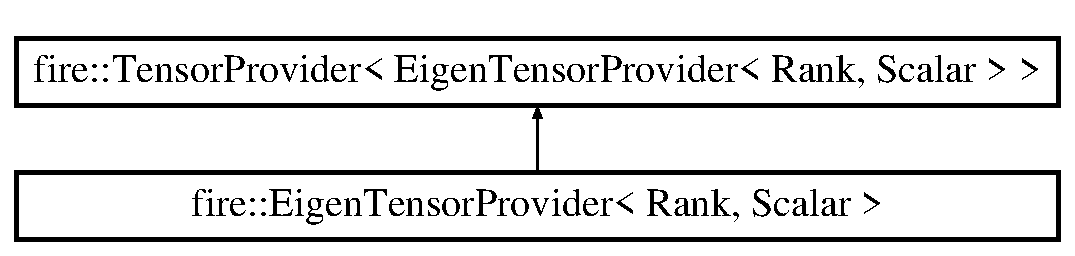
\includegraphics[height=2.000000cm]{a01339}
\end{center}
\end{figure}
\subsection*{Public Member Functions}
\begin{DoxyCompactItemize}
\item 
\hyperlink{a01339_a666937cbdec96978bdd47132a95ab9e6}{Eigen\+Tensor\+Provider} ()
\item 
{\footnotesize template$<$typename ... Dimensions$>$ }\\void \hyperlink{a01339_a5d7147962e2e85c0789b90cced1c6393}{initialize\+Tensor\+Backend} (int first\+Dim, Dimensions ... other\+Dims)
\item 
void \hyperlink{a01339_a284d6bb6a8539c5776e00d2a377d188e}{initialize\+Tensor\+Backend\+With\+Reference} (\hyperlink{a00521_a1bf491fd1c876e2808648b2fd291e3dd}{Tensor\+Reference}$<$ Scalar $>$ \&reference)
\item 
{\footnotesize template$<$typename ... Indices$>$ }\\Scalar \& \hyperlink{a01339_ab664a177792bfb39da25e92b88d6385a}{tensor\+Coefficient} (Indices ... indices)
\item 
bool \hyperlink{a01339_a3e15190363627f4c6b373dc56dd2b4f3}{check\+Equality} (\hyperlink{a00521_a1bf491fd1c876e2808648b2fd291e3dd}{Tensor\+Reference}$<$ Scalar $>$ \&other)
\item 
{\footnotesize template$<$typename Other\+Derived , typename Contraction\+Dims $>$ }\\\hyperlink{a00521_a1bf491fd1c876e2808648b2fd291e3dd}{Tensor\+Reference}$<$ Scalar $>$ \hyperlink{a01339_acd9f39dacb5fd6c35f3f840ed22194e9}{execute\+Contraction} (Other\+Derived \&t2, Contraction\+Dims \&c\+Indices)
\item 
Scalar $\ast$ \hyperlink{a01339_aff5626be9e55f593f0a6b71174ecbd8a}{data} ()
\item 
\hyperlink{a00521_a1bf491fd1c876e2808648b2fd291e3dd}{Tensor\+Reference}$<$ Scalar $>$ \hyperlink{a01339_a957d54e0259b1ea798a47389af4b8379}{add} (\hyperlink{a00521_a1bf491fd1c876e2808648b2fd291e3dd}{Tensor\+Reference}$<$ Scalar $>$ \&other)
\item 
{\footnotesize template$<$typename Init\+List $>$ }\\void \hyperlink{a01339_a3d02dbf7e2d255a1378084aa6459cf25}{set\+Tensor\+Values} (Init\+List \&vals)
\item 
void \hyperlink{a01339_a607ad28d9f0b8b7f639dc1b0693dfd03}{print\+Tensor} (std\+::ostream \&stream)
\item 
void \hyperlink{a01339_a461c3348c66ae011167d8c194c79dce9}{fill\+With\+Random\+Values} ()
\item 
\hyperlink{a00521_a1bf491fd1c876e2808648b2fd291e3dd}{Tensor\+Reference}$<$ Scalar $>$ \hyperlink{a01339_ae526f2376663adc8788ba8f4c04eb6cb}{scalar\+Product} (Scalar \&val)
\item 
{\footnotesize template$<$typename Dim\+Array $>$ }\\\hyperlink{a00521_a1bf491fd1c876e2808648b2fd291e3dd}{Tensor\+Reference}$<$ Scalar $>$ \hyperlink{a01339_a5ffd64a2a2a7b5886b2175d21a46dccf}{reshape\+Tensor} (Dim\+Array \&array)
\item 
\mbox{\Hypertarget{a01339_ac4d85c2ce0bfb666ddb7284241b74dcb}\label{a01339_ac4d85c2ce0bfb666ddb7284241b74dcb}} 
{\footnotesize template$<$typename Dim\+Array $>$ }\\\hyperlink{a00521_a1bf491fd1c876e2808648b2fd291e3dd}{Tensor\+Reference}$<$ Scalar $>$ {\bfseries shuffle\+Tensor} (Dim\+Array \&array)
\item 
\mbox{\Hypertarget{a01339_aa1ba881990a0af6e0a68f8927f94c89d}\label{a01339_aa1ba881990a0af6e0a68f8927f94c89d}} 
std\+::tuple$<$ \hyperlink{a00521_a1bf491fd1c876e2808648b2fd291e3dd}{Tensor\+Reference}$<$ Scalar $>$, \hyperlink{a00521_a1bf491fd1c876e2808648b2fd291e3dd}{Tensor\+Reference}$<$ Scalar $>$, \hyperlink{a00521_a1bf491fd1c876e2808648b2fd291e3dd}{Tensor\+Reference}$<$ Scalar $>$ $>$ {\bfseries compute\+Svd} (\hyperlink{a00521_a1bf491fd1c876e2808648b2fd291e3dd}{Tensor\+Reference}$<$ Scalar $>$ \&ref, double cutoff)
\item 
\mbox{\Hypertarget{a01339_ade4eea42a36aaa42cb8ea85ae3dee711}\label{a01339_ade4eea42a36aaa42cb8ea85ae3dee711}} 
\hyperlink{a00521_a1bf491fd1c876e2808648b2fd291e3dd}{Tensor\+Reference}$<$ Scalar $>$ {\bfseries kron\+Prod} (\hyperlink{a00521_a1bf491fd1c876e2808648b2fd291e3dd}{Tensor\+Reference}$<$ Scalar $>$ \&other)
\end{DoxyCompactItemize}
\subsection*{Static Public Member Functions}
\begin{DoxyCompactItemize}
\item 
static constexpr int \hyperlink{a01339_a68f0ad7ead91dec2ea56f173981465c8}{get\+Rank} ()
\end{DoxyCompactItemize}
\subsection*{Static Public Attributes}
\begin{DoxyCompactItemize}
\item 
static const int \hyperlink{a01339_ae8f0217985d78dba31d7bdb95ace1e43}{rank} = Rank
\end{DoxyCompactItemize}


\subsection{Detailed Description}
\subsubsection*{template$<$const int Rank, typename Scalar = double$>$\newline
class fire\+::\+Eigen\+Tensor\+Provider$<$ Rank, Scalar $>$}

The \hyperlink{a01339}{Eigen\+Tensor\+Provider} is a \hyperlink{a01351}{Tensor\+Provider} that provides tensor data and operations using the Eigen C++ tensor module. 

\subsection{Constructor \& Destructor Documentation}
\mbox{\Hypertarget{a01339_a666937cbdec96978bdd47132a95ab9e6}\label{a01339_a666937cbdec96978bdd47132a95ab9e6}} 
\index{fire\+::\+Eigen\+Tensor\+Provider@{fire\+::\+Eigen\+Tensor\+Provider}!Eigen\+Tensor\+Provider@{Eigen\+Tensor\+Provider}}
\index{Eigen\+Tensor\+Provider@{Eigen\+Tensor\+Provider}!fire\+::\+Eigen\+Tensor\+Provider@{fire\+::\+Eigen\+Tensor\+Provider}}
\subsubsection{\texorpdfstring{Eigen\+Tensor\+Provider()}{EigenTensorProvider()}}
{\footnotesize\ttfamily template$<$const int Rank, typename Scalar = double$>$ \\
\hyperlink{a01339}{fire\+::\+Eigen\+Tensor\+Provider}$<$ Rank, Scalar $>$\+::\hyperlink{a01339}{Eigen\+Tensor\+Provider} (\begin{DoxyParamCaption}{ }\end{DoxyParamCaption})\hspace{0.3cm}{\ttfamily [inline]}}

The Constructor 

\subsection{Member Function Documentation}
\mbox{\Hypertarget{a01339_a957d54e0259b1ea798a47389af4b8379}\label{a01339_a957d54e0259b1ea798a47389af4b8379}} 
\index{fire\+::\+Eigen\+Tensor\+Provider@{fire\+::\+Eigen\+Tensor\+Provider}!add@{add}}
\index{add@{add}!fire\+::\+Eigen\+Tensor\+Provider@{fire\+::\+Eigen\+Tensor\+Provider}}
\subsubsection{\texorpdfstring{add()}{add()}}
{\footnotesize\ttfamily template$<$const int Rank, typename Scalar = double$>$ \\
\hyperlink{a00521_a1bf491fd1c876e2808648b2fd291e3dd}{Tensor\+Reference}$<$Scalar$>$ \hyperlink{a01339}{fire\+::\+Eigen\+Tensor\+Provider}$<$ Rank, Scalar $>$\+::add (\begin{DoxyParamCaption}\item[{\hyperlink{a00521_a1bf491fd1c876e2808648b2fd291e3dd}{Tensor\+Reference}$<$ Scalar $>$ \&}]{other }\end{DoxyParamCaption})\hspace{0.3cm}{\ttfamily [inline]}}

Return a Tensor\+Reference representing the sum of this Eigen \hyperlink{a01347}{Tensor} and an Eigen \hyperlink{a01347}{Tensor} represented by the other Tensor\+Reference.


\begin{DoxyParams}{Parameters}
{\em other} & Tensor\+Reference view of the other \hyperlink{a01347}{Tensor} \\
\hline
\end{DoxyParams}
\begin{DoxyReturn}{Returns}
result A new Tensor\+Reference representing the sum of this and other. 
\end{DoxyReturn}
\mbox{\Hypertarget{a01339_a3e15190363627f4c6b373dc56dd2b4f3}\label{a01339_a3e15190363627f4c6b373dc56dd2b4f3}} 
\index{fire\+::\+Eigen\+Tensor\+Provider@{fire\+::\+Eigen\+Tensor\+Provider}!check\+Equality@{check\+Equality}}
\index{check\+Equality@{check\+Equality}!fire\+::\+Eigen\+Tensor\+Provider@{fire\+::\+Eigen\+Tensor\+Provider}}
\subsubsection{\texorpdfstring{check\+Equality()}{checkEquality()}}
{\footnotesize\ttfamily template$<$const int Rank, typename Scalar = double$>$ \\
bool \hyperlink{a01339}{fire\+::\+Eigen\+Tensor\+Provider}$<$ Rank, Scalar $>$\+::check\+Equality (\begin{DoxyParamCaption}\item[{\hyperlink{a00521_a1bf491fd1c876e2808648b2fd291e3dd}{Tensor\+Reference}$<$ Scalar $>$ \&}]{other }\end{DoxyParamCaption})\hspace{0.3cm}{\ttfamily [inline]}}

Return true if the provided Tensor\+Reference as a tensor is equal to this tensor.


\begin{DoxyParams}{Parameters}
{\em other} & Tensor\+Reference view of the other \hyperlink{a01347}{Tensor} \\
\hline
\end{DoxyParams}
\begin{DoxyReturn}{Returns}
equal A boolean indicating if these Tensors are equal 
\end{DoxyReturn}
\mbox{\Hypertarget{a01339_aff5626be9e55f593f0a6b71174ecbd8a}\label{a01339_aff5626be9e55f593f0a6b71174ecbd8a}} 
\index{fire\+::\+Eigen\+Tensor\+Provider@{fire\+::\+Eigen\+Tensor\+Provider}!data@{data}}
\index{data@{data}!fire\+::\+Eigen\+Tensor\+Provider@{fire\+::\+Eigen\+Tensor\+Provider}}
\subsubsection{\texorpdfstring{data()}{data()}}
{\footnotesize\ttfamily template$<$const int Rank, typename Scalar = double$>$ \\
Scalar$\ast$ \hyperlink{a01339}{fire\+::\+Eigen\+Tensor\+Provider}$<$ Rank, Scalar $>$\+::data (\begin{DoxyParamCaption}{ }\end{DoxyParamCaption})\hspace{0.3cm}{\ttfamily [inline]}}

Return the 1-\/D array wrapped by this Eigen \hyperlink{a01347}{Tensor}

\begin{DoxyReturn}{Returns}
data 1-\/D array of data representing the tensor in this \hyperlink{a01351}{Tensor\+Provider} 
\end{DoxyReturn}
\mbox{\Hypertarget{a01339_acd9f39dacb5fd6c35f3f840ed22194e9}\label{a01339_acd9f39dacb5fd6c35f3f840ed22194e9}} 
\index{fire\+::\+Eigen\+Tensor\+Provider@{fire\+::\+Eigen\+Tensor\+Provider}!execute\+Contraction@{execute\+Contraction}}
\index{execute\+Contraction@{execute\+Contraction}!fire\+::\+Eigen\+Tensor\+Provider@{fire\+::\+Eigen\+Tensor\+Provider}}
\subsubsection{\texorpdfstring{execute\+Contraction()}{executeContraction()}}
{\footnotesize\ttfamily template$<$const int Rank, typename Scalar = double$>$ \\
template$<$typename Other\+Derived , typename Contraction\+Dims $>$ \\
\hyperlink{a00521_a1bf491fd1c876e2808648b2fd291e3dd}{Tensor\+Reference}$<$Scalar$>$ \hyperlink{a01339}{fire\+::\+Eigen\+Tensor\+Provider}$<$ Rank, Scalar $>$\+::execute\+Contraction (\begin{DoxyParamCaption}\item[{Other\+Derived \&}]{t2,  }\item[{Contraction\+Dims \&}]{c\+Indices }\end{DoxyParamCaption})\hspace{0.3cm}{\ttfamily [inline]}}

Compute the tensor contraction of this Eigen \hyperlink{a01347}{Tensor} with the provided Other \hyperlink{a01347}{Tensor}.


\begin{DoxyParams}{Parameters}
{\em t2} & The other \hyperlink{a01347}{Tensor} \\
\hline
{\em indices} & The contraction indices. \\
\hline
\end{DoxyParams}
\begin{DoxyReturn}{Returns}
result The contraction result as a Tensor\+Reference 
\end{DoxyReturn}
\mbox{\Hypertarget{a01339_a461c3348c66ae011167d8c194c79dce9}\label{a01339_a461c3348c66ae011167d8c194c79dce9}} 
\index{fire\+::\+Eigen\+Tensor\+Provider@{fire\+::\+Eigen\+Tensor\+Provider}!fill\+With\+Random\+Values@{fill\+With\+Random\+Values}}
\index{fill\+With\+Random\+Values@{fill\+With\+Random\+Values}!fire\+::\+Eigen\+Tensor\+Provider@{fire\+::\+Eigen\+Tensor\+Provider}}
\subsubsection{\texorpdfstring{fill\+With\+Random\+Values()}{fillWithRandomValues()}}
{\footnotesize\ttfamily template$<$const int Rank, typename Scalar = double$>$ \\
void \hyperlink{a01339}{fire\+::\+Eigen\+Tensor\+Provider}$<$ Rank, Scalar $>$\+::fill\+With\+Random\+Values (\begin{DoxyParamCaption}{ }\end{DoxyParamCaption})\hspace{0.3cm}{\ttfamily [inline]}}

Set the Eigen \hyperlink{a01347}{Tensor} values to random values. \mbox{\Hypertarget{a01339_a68f0ad7ead91dec2ea56f173981465c8}\label{a01339_a68f0ad7ead91dec2ea56f173981465c8}} 
\index{fire\+::\+Eigen\+Tensor\+Provider@{fire\+::\+Eigen\+Tensor\+Provider}!get\+Rank@{get\+Rank}}
\index{get\+Rank@{get\+Rank}!fire\+::\+Eigen\+Tensor\+Provider@{fire\+::\+Eigen\+Tensor\+Provider}}
\subsubsection{\texorpdfstring{get\+Rank()}{getRank()}}
{\footnotesize\ttfamily template$<$const int Rank, typename Scalar = double$>$ \\
static constexpr int \hyperlink{a01339}{fire\+::\+Eigen\+Tensor\+Provider}$<$ Rank, Scalar $>$\+::get\+Rank (\begin{DoxyParamCaption}{ }\end{DoxyParamCaption})\hspace{0.3cm}{\ttfamily [inline]}, {\ttfamily [static]}}

Return the rank of this Eigen \hyperlink{a01347}{Tensor}

\begin{DoxyReturn}{Returns}
rank The rank of this \hyperlink{a01347}{Tensor} 
\end{DoxyReturn}
\mbox{\Hypertarget{a01339_a5d7147962e2e85c0789b90cced1c6393}\label{a01339_a5d7147962e2e85c0789b90cced1c6393}} 
\index{fire\+::\+Eigen\+Tensor\+Provider@{fire\+::\+Eigen\+Tensor\+Provider}!initialize\+Tensor\+Backend@{initialize\+Tensor\+Backend}}
\index{initialize\+Tensor\+Backend@{initialize\+Tensor\+Backend}!fire\+::\+Eigen\+Tensor\+Provider@{fire\+::\+Eigen\+Tensor\+Provider}}
\subsubsection{\texorpdfstring{initialize\+Tensor\+Backend()}{initializeTensorBackend()}}
{\footnotesize\ttfamily template$<$const int Rank, typename Scalar = double$>$ \\
template$<$typename ... Dimensions$>$ \\
void \hyperlink{a01339}{fire\+::\+Eigen\+Tensor\+Provider}$<$ Rank, Scalar $>$\+::initialize\+Tensor\+Backend (\begin{DoxyParamCaption}\item[{int}]{first\+Dim,  }\item[{Dimensions ...}]{other\+Dims }\end{DoxyParamCaption})\hspace{0.3cm}{\ttfamily [inline]}}

Initialize the Eigen \hyperlink{a01347}{Tensor} with all zeros. 
\begin{DoxyParams}{Parameters}
{\em first\+Dim} & \\
\hline
{\em other\+Dims} & \\
\hline
\end{DoxyParams}
\mbox{\Hypertarget{a01339_a284d6bb6a8539c5776e00d2a377d188e}\label{a01339_a284d6bb6a8539c5776e00d2a377d188e}} 
\index{fire\+::\+Eigen\+Tensor\+Provider@{fire\+::\+Eigen\+Tensor\+Provider}!initialize\+Tensor\+Backend\+With\+Reference@{initialize\+Tensor\+Backend\+With\+Reference}}
\index{initialize\+Tensor\+Backend\+With\+Reference@{initialize\+Tensor\+Backend\+With\+Reference}!fire\+::\+Eigen\+Tensor\+Provider@{fire\+::\+Eigen\+Tensor\+Provider}}
\subsubsection{\texorpdfstring{initialize\+Tensor\+Backend\+With\+Reference()}{initializeTensorBackendWithReference()}}
{\footnotesize\ttfamily template$<$const int Rank, typename Scalar = double$>$ \\
void \hyperlink{a01339}{fire\+::\+Eigen\+Tensor\+Provider}$<$ Rank, Scalar $>$\+::initialize\+Tensor\+Backend\+With\+Reference (\begin{DoxyParamCaption}\item[{\hyperlink{a00521_a1bf491fd1c876e2808648b2fd291e3dd}{Tensor\+Reference}$<$ Scalar $>$ \&}]{reference }\end{DoxyParamCaption})\hspace{0.3cm}{\ttfamily [inline]}}

Initialize the Eigen \hyperlink{a01347}{Tensor} from an existing Tensor\+Reference 
\begin{DoxyParams}{Parameters}
{\em reference} & \\
\hline
\end{DoxyParams}
\mbox{\Hypertarget{a01339_a607ad28d9f0b8b7f639dc1b0693dfd03}\label{a01339_a607ad28d9f0b8b7f639dc1b0693dfd03}} 
\index{fire\+::\+Eigen\+Tensor\+Provider@{fire\+::\+Eigen\+Tensor\+Provider}!print\+Tensor@{print\+Tensor}}
\index{print\+Tensor@{print\+Tensor}!fire\+::\+Eigen\+Tensor\+Provider@{fire\+::\+Eigen\+Tensor\+Provider}}
\subsubsection{\texorpdfstring{print\+Tensor()}{printTensor()}}
{\footnotesize\ttfamily template$<$const int Rank, typename Scalar = double$>$ \\
void \hyperlink{a01339}{fire\+::\+Eigen\+Tensor\+Provider}$<$ Rank, Scalar $>$\+::print\+Tensor (\begin{DoxyParamCaption}\item[{std\+::ostream \&}]{stream }\end{DoxyParamCaption})\hspace{0.3cm}{\ttfamily [inline]}}

Output this Eigen \hyperlink{a01347}{Tensor} to the provided output stream.


\begin{DoxyParams}{Parameters}
{\em output\+Stream} & The output stream to write the tensor to. \\
\hline
\end{DoxyParams}
\mbox{\Hypertarget{a01339_a5ffd64a2a2a7b5886b2175d21a46dccf}\label{a01339_a5ffd64a2a2a7b5886b2175d21a46dccf}} 
\index{fire\+::\+Eigen\+Tensor\+Provider@{fire\+::\+Eigen\+Tensor\+Provider}!reshape\+Tensor@{reshape\+Tensor}}
\index{reshape\+Tensor@{reshape\+Tensor}!fire\+::\+Eigen\+Tensor\+Provider@{fire\+::\+Eigen\+Tensor\+Provider}}
\subsubsection{\texorpdfstring{reshape\+Tensor()}{reshapeTensor()}}
{\footnotesize\ttfamily template$<$const int Rank, typename Scalar = double$>$ \\
template$<$typename Dim\+Array $>$ \\
\hyperlink{a00521_a1bf491fd1c876e2808648b2fd291e3dd}{Tensor\+Reference}$<$Scalar$>$ \hyperlink{a01339}{fire\+::\+Eigen\+Tensor\+Provider}$<$ Rank, Scalar $>$\+::reshape\+Tensor (\begin{DoxyParamCaption}\item[{Dim\+Array \&}]{array }\end{DoxyParamCaption})\hspace{0.3cm}{\ttfamily [inline]}}

Reshape the Eigen \hyperlink{a01347}{Tensor} with a new array of dimensions


\begin{DoxyParams}{Parameters}
{\em array} & Array of new dimensions for each rank index \\
\hline
\end{DoxyParams}
\begin{DoxyReturn}{Returns}
reshaped\+Tensor A Tensor\+Reference representing new reshaped tensor. 
\end{DoxyReturn}
\mbox{\Hypertarget{a01339_ae526f2376663adc8788ba8f4c04eb6cb}\label{a01339_ae526f2376663adc8788ba8f4c04eb6cb}} 
\index{fire\+::\+Eigen\+Tensor\+Provider@{fire\+::\+Eigen\+Tensor\+Provider}!scalar\+Product@{scalar\+Product}}
\index{scalar\+Product@{scalar\+Product}!fire\+::\+Eigen\+Tensor\+Provider@{fire\+::\+Eigen\+Tensor\+Provider}}
\subsubsection{\texorpdfstring{scalar\+Product()}{scalarProduct()}}
{\footnotesize\ttfamily template$<$const int Rank, typename Scalar = double$>$ \\
\hyperlink{a00521_a1bf491fd1c876e2808648b2fd291e3dd}{Tensor\+Reference}$<$Scalar$>$ \hyperlink{a01339}{fire\+::\+Eigen\+Tensor\+Provider}$<$ Rank, Scalar $>$\+::scalar\+Product (\begin{DoxyParamCaption}\item[{Scalar \&}]{val }\end{DoxyParamCaption})\hspace{0.3cm}{\ttfamily [inline]}}

Multiply all elements of this Eigen \hyperlink{a01347}{Tensor} by the provided Scalar.


\begin{DoxyParams}{Parameters}
{\em val} & Scalar to multiply this tensor by. \\
\hline
\end{DoxyParams}
\begin{DoxyReturn}{Returns}
result A Tensor\+Reference representing the result 
\end{DoxyReturn}
\mbox{\Hypertarget{a01339_a3d02dbf7e2d255a1378084aa6459cf25}\label{a01339_a3d02dbf7e2d255a1378084aa6459cf25}} 
\index{fire\+::\+Eigen\+Tensor\+Provider@{fire\+::\+Eigen\+Tensor\+Provider}!set\+Tensor\+Values@{set\+Tensor\+Values}}
\index{set\+Tensor\+Values@{set\+Tensor\+Values}!fire\+::\+Eigen\+Tensor\+Provider@{fire\+::\+Eigen\+Tensor\+Provider}}
\subsubsection{\texorpdfstring{set\+Tensor\+Values()}{setTensorValues()}}
{\footnotesize\ttfamily template$<$const int Rank, typename Scalar = double$>$ \\
template$<$typename Init\+List $>$ \\
void \hyperlink{a01339}{fire\+::\+Eigen\+Tensor\+Provider}$<$ Rank, Scalar $>$\+::set\+Tensor\+Values (\begin{DoxyParamCaption}\item[{Init\+List \&}]{vals }\end{DoxyParamCaption})\hspace{0.3cm}{\ttfamily [inline]}}

Set the Eigen \hyperlink{a01347}{Tensor} values using nested initializer\+\_\+list


\begin{DoxyParams}{Parameters}
{\em vals} & The values as a nest std\+::initializer\+\_\+lists \\
\hline
\end{DoxyParams}
\mbox{\Hypertarget{a01339_ab664a177792bfb39da25e92b88d6385a}\label{a01339_ab664a177792bfb39da25e92b88d6385a}} 
\index{fire\+::\+Eigen\+Tensor\+Provider@{fire\+::\+Eigen\+Tensor\+Provider}!tensor\+Coefficient@{tensor\+Coefficient}}
\index{tensor\+Coefficient@{tensor\+Coefficient}!fire\+::\+Eigen\+Tensor\+Provider@{fire\+::\+Eigen\+Tensor\+Provider}}
\subsubsection{\texorpdfstring{tensor\+Coefficient()}{tensorCoefficient()}}
{\footnotesize\ttfamily template$<$const int Rank, typename Scalar = double$>$ \\
template$<$typename ... Indices$>$ \\
Scalar\& \hyperlink{a01339}{fire\+::\+Eigen\+Tensor\+Provider}$<$ Rank, Scalar $>$\+::tensor\+Coefficient (\begin{DoxyParamCaption}\item[{Indices ...}]{indices }\end{DoxyParamCaption})\hspace{0.3cm}{\ttfamily [inline]}}

Return the coefficient at the given tensor indices.


\begin{DoxyParams}{Parameters}
{\em indices} & The indices for the desired value \\
\hline
\end{DoxyParams}
\begin{DoxyReturn}{Returns}
val The value at the indices. 
\end{DoxyReturn}


\subsection{Member Data Documentation}
\mbox{\Hypertarget{a01339_ae8f0217985d78dba31d7bdb95ace1e43}\label{a01339_ae8f0217985d78dba31d7bdb95ace1e43}} 
\index{fire\+::\+Eigen\+Tensor\+Provider@{fire\+::\+Eigen\+Tensor\+Provider}!rank@{rank}}
\index{rank@{rank}!fire\+::\+Eigen\+Tensor\+Provider@{fire\+::\+Eigen\+Tensor\+Provider}}
\subsubsection{\texorpdfstring{rank}{rank}}
{\footnotesize\ttfamily template$<$const int Rank, typename Scalar = double$>$ \\
const int \hyperlink{a01339}{fire\+::\+Eigen\+Tensor\+Provider}$<$ Rank, Scalar $>$\+::rank = Rank\hspace{0.3cm}{\ttfamily [static]}}

Static reference to the rank of the tensor wrapped by this provider 

The documentation for this class was generated from the following file\+:\begin{DoxyCompactItemize}
\item 
Eigen\+Tensor\+Provider.\+hpp\end{DoxyCompactItemize}

\hypertarget{a01123}{}\section{xacc\+:\+:Register\+Algorithm\+Generator$<$ T $>$ Class Template Reference}
\label{a01123}\index{xacc\+::\+Register\+Algorithm\+Generator$<$ T $>$@{xacc\+::\+Register\+Algorithm\+Generator$<$ T $>$}}


{\ttfamily \#include $<$Algorithm\+Generator.\+hpp$>$}

\subsection*{Public Member Functions}
\begin{DoxyCompactItemize}
\item 
\mbox{\Hypertarget{a01123_af439cc4d7c8d6628a979129a5c1411df}\label{a01123_af439cc4d7c8d6628a979129a5c1411df}} 
{\bfseries Register\+Algorithm\+Generator} (const std\+::string \&name)
\end{DoxyCompactItemize}


\subsection{Detailed Description}
\subsubsection*{template$<$typename T$>$\newline
class xacc\+::\+Register\+Algorithm\+Generator$<$ T $>$}

\hyperlink{a01123}{Register\+Algorithm\+Generator} is a convenience class for registering custom derived \hyperlink{a01119}{Algorithm\+Generator} classes.

Creators of \hyperlink{a01119}{Algorithm\+Generator} subclasses create an instance of this class with their \hyperlink{a01119}{Algorithm\+Generator} subclass as the template parameter to register their \hyperlink{a01119}{Algorithm\+Generator} with X\+A\+CC. This instance must be created in the C\+PP implementation file for the \hyperlink{a01119}{Algorithm\+Generator} and at global scope. 

The documentation for this class was generated from the following file\+:\begin{DoxyCompactItemize}
\item 
Algorithm\+Generator.\+hpp\end{DoxyCompactItemize}

\hypertarget{a01387}{}\section{C\+Simple\+Ini\+Templ$<$ S\+I\+\_\+\+C\+H\+AR, S\+I\+\_\+\+S\+T\+R\+L\+E\+SS, S\+I\+\_\+\+C\+O\+N\+V\+E\+R\+T\+ER $>$\+:\+:Entry Struct Reference}
\label{a01387}\index{C\+Simple\+Ini\+Templ$<$ S\+I\+\_\+\+C\+H\+A\+R, S\+I\+\_\+\+S\+T\+R\+L\+E\+S\+S, S\+I\+\_\+\+C\+O\+N\+V\+E\+R\+T\+E\+R $>$\+::\+Entry@{C\+Simple\+Ini\+Templ$<$ S\+I\+\_\+\+C\+H\+A\+R, S\+I\+\_\+\+S\+T\+R\+L\+E\+S\+S, S\+I\+\_\+\+C\+O\+N\+V\+E\+R\+T\+E\+R $>$\+::\+Entry}}


{\ttfamily \#include $<$Simple\+Ini.\+h$>$}

\subsection*{Classes}
\begin{DoxyCompactItemize}
\item 
struct \hyperlink{a01391}{Key\+Order}
\item 
struct \hyperlink{a01395}{Load\+Order}
\end{DoxyCompactItemize}
\subsection*{Public Member Functions}
\begin{DoxyCompactItemize}
\item 
\mbox{\Hypertarget{a01387_a20fc446e1f56f562333042a19bb57c9c}\label{a01387_a20fc446e1f56f562333042a19bb57c9c}} 
{\bfseries Entry} (const S\+I\+\_\+\+C\+H\+AR $\ast$a\+\_\+psz\+Item=N\+U\+LL, int a\+\_\+n\+Order=0)
\item 
\mbox{\Hypertarget{a01387_aaa6fc487377a2fc91dc4f0b83e572996}\label{a01387_aaa6fc487377a2fc91dc4f0b83e572996}} 
{\bfseries Entry} (const S\+I\+\_\+\+C\+H\+AR $\ast$a\+\_\+psz\+Item, const S\+I\+\_\+\+C\+H\+AR $\ast$a\+\_\+psz\+Comment, int a\+\_\+n\+Order)
\item 
\mbox{\Hypertarget{a01387_afbe8b9d3c87d5de3c6aa8d8984f011f6}\label{a01387_afbe8b9d3c87d5de3c6aa8d8984f011f6}} 
{\bfseries Entry} (const \hyperlink{a01387}{Entry} \&rhs)
\item 
\mbox{\Hypertarget{a01387_a7f4dd11cc944c140d751ae22ef6cd034}\label{a01387_a7f4dd11cc944c140d751ae22ef6cd034}} 
\hyperlink{a01387}{Entry} \& {\bfseries operator=} (const \hyperlink{a01387}{Entry} \&rhs)
\end{DoxyCompactItemize}
\subsection*{Public Attributes}
\begin{DoxyCompactItemize}
\item 
\mbox{\Hypertarget{a01387_a0f987914bf6076156c2a7c40e8e09c89}\label{a01387_a0f987914bf6076156c2a7c40e8e09c89}} 
const S\+I\+\_\+\+C\+H\+AR $\ast$ {\bfseries p\+Item}
\item 
\mbox{\Hypertarget{a01387_a84364bcded2d32c5ae4241bf197a74c4}\label{a01387_a84364bcded2d32c5ae4241bf197a74c4}} 
const S\+I\+\_\+\+C\+H\+AR $\ast$ {\bfseries p\+Comment}
\item 
\mbox{\Hypertarget{a01387_ac08ed1fec5743b35aebfa8635e1bdb5a}\label{a01387_ac08ed1fec5743b35aebfa8635e1bdb5a}} 
int {\bfseries n\+Order}
\end{DoxyCompactItemize}


\subsection{Detailed Description}
\subsubsection*{template$<$class S\+I\+\_\+\+C\+H\+AR, class S\+I\+\_\+\+S\+T\+R\+L\+E\+SS, class S\+I\+\_\+\+C\+O\+N\+V\+E\+R\+T\+ER$>$\newline
struct C\+Simple\+Ini\+Templ$<$ S\+I\+\_\+\+C\+H\+A\+R, S\+I\+\_\+\+S\+T\+R\+L\+E\+S\+S, S\+I\+\_\+\+C\+O\+N\+V\+E\+R\+T\+E\+R $>$\+::\+Entry}

key entry 

The documentation for this struct was generated from the following file\+:\begin{DoxyCompactItemize}
\item 
Simple\+Ini.\+h\end{DoxyCompactItemize}

\hypertarget{a01087}{}\section{xacc\+:\+:Accelerator Class Reference}
\label{a01087}\index{xacc\+::\+Accelerator@{xacc\+::\+Accelerator}}


{\ttfamily \#include $<$Accelerator.\+hpp$>$}

Inheritance diagram for xacc\+:\+:Accelerator\+:\begin{figure}[H]
\begin{center}
\leavevmode
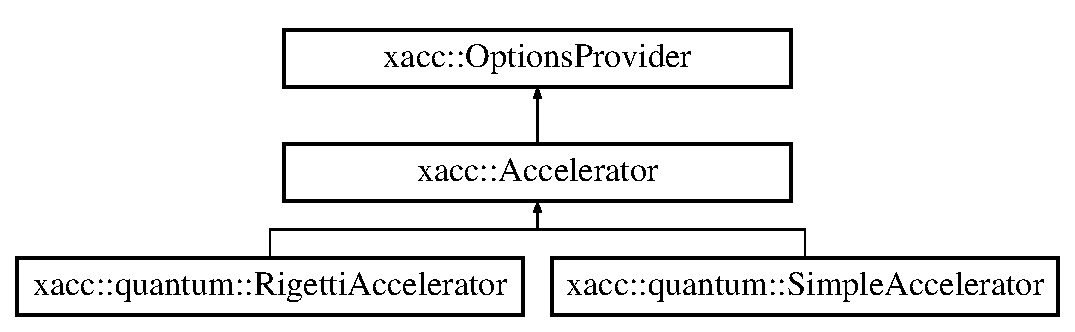
\includegraphics[height=3.000000cm]{a01087}
\end{center}
\end{figure}
\subsection*{Public Member Functions}
\begin{DoxyCompactItemize}
\item 
virtual Accelerator\+Type \hyperlink{a01087_aaffc3e4bb9880eb5041b1b58ee4c2665}{get\+Type} ()=0
\item 
virtual std\+::vector$<$ \hyperlink{a01155}{I\+R\+Transformation} $>$ \hyperlink{a01087_ad6e4a642dcb24e552675bcbeff1e1b04}{get\+I\+R\+Transformations} ()=0
\item 
virtual void \hyperlink{a01087_a89b3f3e6294f228abf03a410b0fb1674}{execute} (std\+::shared\+\_\+ptr$<$ \hyperlink{a01099}{Accelerator\+Buffer} $>$ buffer, const std\+::shared\+\_\+ptr$<$ \hyperlink{a01127}{Function} $>$ function)=0
\item 
virtual std\+::shared\+\_\+ptr$<$ \hyperlink{a01099}{Accelerator\+Buffer} $>$ \hyperlink{a01087_a064a2dbd58338364115c260267806945}{create\+Buffer} (const std\+::string \&var\+Id, const int size)=0
\item 
virtual std\+::shared\+\_\+ptr$<$ \hyperlink{a01099}{Accelerator\+Buffer} $>$ \hyperlink{a01087_ab3820be326e28a553fed1a824f4d41d0}{get\+Buffer} (const std\+::string \&varid)
\item 
virtual std\+::vector$<$ std\+::string $>$ \hyperlink{a01087_ae1463d7e405df89fa4af47e8922f4b82}{get\+Allocated\+Buffer\+Names} ()
\item 
virtual std\+::shared\+\_\+ptr$<$ options\+\_\+description $>$ \hyperlink{a01087_a98c9eda6b54367c75667ecfbbf167979}{get\+Options} ()
\item 
virtual \hyperlink{a01087_aed88ab0d71b765f0b0f512684ccd4b55}{$\sim$\+Accelerator} ()
\end{DoxyCompactItemize}
\subsection*{Protected Member Functions}
\begin{DoxyCompactItemize}
\item 
virtual bool \hyperlink{a01087_ae51584850faeec77299058383977ddeb}{is\+Valid\+Buffer\+Size} (const int N\+Bits)=0
\item 
void \hyperlink{a01087_ac3e781f42ec25e460174d4c41ea26b94}{store\+Buffer} (const std\+::string \&id, std\+::shared\+\_\+ptr$<$ \hyperlink{a01099}{Accelerator\+Buffer} $>$ b)
\end{DoxyCompactItemize}


\subsection{Detailed Description}
The \hyperlink{a01087}{Accelerator} class provides a high-\/level abstraction for X\+A\+CC\textquotesingle{}s interaction with attached post-\/exascale accelerators (quantum and neuromorphic processing units).

Derived Accelerators must provide a valid execute implementation that takes X\+A\+CC \hyperlink{a01151}{IR} and executes it on the attached hardware or simulator.

Derived Accelerators must provide a list of \hyperlink{a01155}{I\+R\+Transformation} instances that transform X\+A\+CC \hyperlink{a01151}{IR} to be amenable to execution on the hardware.

Derived Accelerators must provide implementations of create\+Buffer that provide a valid \hyperlink{a01099}{Accelerator\+Buffer} instance modeling the hardware memory or bits being computed on. Upon creating an \hyperlink{a01099}{Accelerator\+Buffer}, derived \hyperlink{a01087}{Accelerator} implementations must call the protected store\+Buffer method to store the \hyperlink{a01099}{Accelerator\+Buffer} for future reference by Compilers and clients of \hyperlink{a01087}{Accelerator}.

\begin{DoxyAuthor}{Author}
Alex Mc\+Caskey 
\end{DoxyAuthor}


\subsection{Constructor \& Destructor Documentation}
\mbox{\Hypertarget{a01087_aed88ab0d71b765f0b0f512684ccd4b55}\label{a01087_aed88ab0d71b765f0b0f512684ccd4b55}} 
\index{xacc\+::\+Accelerator@{xacc\+::\+Accelerator}!````~Accelerator@{$\sim$\+Accelerator}}
\index{````~Accelerator@{$\sim$\+Accelerator}!xacc\+::\+Accelerator@{xacc\+::\+Accelerator}}
\subsubsection{\texorpdfstring{$\sim$\+Accelerator()}{~Accelerator()}}
{\footnotesize\ttfamily virtual xacc\+::\+Accelerator\+::$\sim$\+Accelerator (\begin{DoxyParamCaption}{ }\end{DoxyParamCaption})\hspace{0.3cm}{\ttfamily [inline]}, {\ttfamily [virtual]}}

Destructor 

\subsection{Member Function Documentation}
\mbox{\Hypertarget{a01087_a064a2dbd58338364115c260267806945}\label{a01087_a064a2dbd58338364115c260267806945}} 
\index{xacc\+::\+Accelerator@{xacc\+::\+Accelerator}!create\+Buffer@{create\+Buffer}}
\index{create\+Buffer@{create\+Buffer}!xacc\+::\+Accelerator@{xacc\+::\+Accelerator}}
\subsubsection{\texorpdfstring{create\+Buffer()}{createBuffer()}}
{\footnotesize\ttfamily virtual std\+::shared\+\_\+ptr$<$\hyperlink{a01099}{Accelerator\+Buffer}$>$ xacc\+::\+Accelerator\+::create\+Buffer (\begin{DoxyParamCaption}\item[{const std\+::string \&}]{var\+Id,  }\item[{const int}]{size }\end{DoxyParamCaption})\hspace{0.3cm}{\ttfamily [pure virtual]}}

Create, store, and return an \hyperlink{a01099}{Accelerator\+Buffer} with the given variable id string and of the given number of bits. The string id serves as a unique identifier for future lookups and reuse of the \hyperlink{a01099}{Accelerator\+Buffer}.


\begin{DoxyParams}{Parameters}
{\em var\+Id} & The variable name of the created buffer \\
\hline
{\em size} & The number of bits in the created buffer \\
\hline
\end{DoxyParams}
\begin{DoxyReturn}{Returns}
buffer The buffer instance created. 
\end{DoxyReturn}


Implemented in \hyperlink{a00919_a731551c94b1abef40d2cf032e8712df6}{xacc\+::quantum\+::\+Rigetti\+Accelerator}, and \hyperlink{a00943_adb9393692e9f484df241aa5d014030d1}{xacc\+::quantum\+::\+Simple\+Accelerator}.

\mbox{\Hypertarget{a01087_a89b3f3e6294f228abf03a410b0fb1674}\label{a01087_a89b3f3e6294f228abf03a410b0fb1674}} 
\index{xacc\+::\+Accelerator@{xacc\+::\+Accelerator}!execute@{execute}}
\index{execute@{execute}!xacc\+::\+Accelerator@{xacc\+::\+Accelerator}}
\subsubsection{\texorpdfstring{execute()}{execute()}}
{\footnotesize\ttfamily virtual void xacc\+::\+Accelerator\+::execute (\begin{DoxyParamCaption}\item[{std\+::shared\+\_\+ptr$<$ \hyperlink{a01099}{Accelerator\+Buffer} $>$}]{buffer,  }\item[{const std\+::shared\+\_\+ptr$<$ \hyperlink{a01127}{Function} $>$}]{function }\end{DoxyParamCaption})\hspace{0.3cm}{\ttfamily [pure virtual]}}

Execute the provided X\+A\+CC \hyperlink{a01151}{IR} \hyperlink{a01127}{Function} on the provided \hyperlink{a01099}{Accelerator\+Buffer}.


\begin{DoxyParams}{Parameters}
{\em buffer} & The buffer of bits this \hyperlink{a01087}{Accelerator} should operate on. \\
\hline
{\em function} & The kernel to execute. \\
\hline
\end{DoxyParams}
\mbox{\Hypertarget{a01087_ae1463d7e405df89fa4af47e8922f4b82}\label{a01087_ae1463d7e405df89fa4af47e8922f4b82}} 
\index{xacc\+::\+Accelerator@{xacc\+::\+Accelerator}!get\+Allocated\+Buffer\+Names@{get\+Allocated\+Buffer\+Names}}
\index{get\+Allocated\+Buffer\+Names@{get\+Allocated\+Buffer\+Names}!xacc\+::\+Accelerator@{xacc\+::\+Accelerator}}
\subsubsection{\texorpdfstring{get\+Allocated\+Buffer\+Names()}{getAllocatedBufferNames()}}
{\footnotesize\ttfamily virtual std\+::vector$<$std\+::string$>$ xacc\+::\+Accelerator\+::get\+Allocated\+Buffer\+Names (\begin{DoxyParamCaption}{ }\end{DoxyParamCaption})\hspace{0.3cm}{\ttfamily [inline]}, {\ttfamily [virtual]}}

Return all allocated \hyperlink{a01099}{Accelerator\+Buffer} variable names.

\begin{DoxyReturn}{Returns}
var\+Names The buffer variable names 
\end{DoxyReturn}
\mbox{\Hypertarget{a01087_ab3820be326e28a553fed1a824f4d41d0}\label{a01087_ab3820be326e28a553fed1a824f4d41d0}} 
\index{xacc\+::\+Accelerator@{xacc\+::\+Accelerator}!get\+Buffer@{get\+Buffer}}
\index{get\+Buffer@{get\+Buffer}!xacc\+::\+Accelerator@{xacc\+::\+Accelerator}}
\subsubsection{\texorpdfstring{get\+Buffer()}{getBuffer()}}
{\footnotesize\ttfamily virtual std\+::shared\+\_\+ptr$<$\hyperlink{a01099}{Accelerator\+Buffer}$>$ xacc\+::\+Accelerator\+::get\+Buffer (\begin{DoxyParamCaption}\item[{const std\+::string \&}]{varid }\end{DoxyParamCaption})\hspace{0.3cm}{\ttfamily [inline]}, {\ttfamily [virtual]}}

Return the stored \hyperlink{a01099}{Accelerator\+Buffer} with the provided string id.


\begin{DoxyParams}{Parameters}
{\em varid} & The variable name of the created buffer \\
\hline
\end{DoxyParams}
\begin{DoxyReturn}{Returns}
buffer The buffer with given varid. 
\end{DoxyReturn}
\mbox{\Hypertarget{a01087_ad6e4a642dcb24e552675bcbeff1e1b04}\label{a01087_ad6e4a642dcb24e552675bcbeff1e1b04}} 
\index{xacc\+::\+Accelerator@{xacc\+::\+Accelerator}!get\+I\+R\+Transformations@{get\+I\+R\+Transformations}}
\index{get\+I\+R\+Transformations@{get\+I\+R\+Transformations}!xacc\+::\+Accelerator@{xacc\+::\+Accelerator}}
\subsubsection{\texorpdfstring{get\+I\+R\+Transformations()}{getIRTransformations()}}
{\footnotesize\ttfamily virtual std\+::vector$<$\hyperlink{a01155}{I\+R\+Transformation}$>$ xacc\+::\+Accelerator\+::get\+I\+R\+Transformations (\begin{DoxyParamCaption}{ }\end{DoxyParamCaption})\hspace{0.3cm}{\ttfamily [pure virtual]}}

Return any \hyperlink{a01151}{IR} Transformations that must be applied to ensure the compiled \hyperlink{a01151}{IR} is amenable to execution on this \hyperlink{a01087}{Accelerator}.

\begin{DoxyReturn}{Returns}
transformations The \hyperlink{a01151}{IR} transformations this \hyperlink{a01087}{Accelerator} exposes 
\end{DoxyReturn}


Implemented in \hyperlink{a00919_a443683a1dfb000603c640b2ee303cf66}{xacc\+::quantum\+::\+Rigetti\+Accelerator}, and \hyperlink{a00943_afc49c9e7973ba6c6ff9761c36198323d}{xacc\+::quantum\+::\+Simple\+Accelerator}.

\mbox{\Hypertarget{a01087_a98c9eda6b54367c75667ecfbbf167979}\label{a01087_a98c9eda6b54367c75667ecfbbf167979}} 
\index{xacc\+::\+Accelerator@{xacc\+::\+Accelerator}!get\+Options@{get\+Options}}
\index{get\+Options@{get\+Options}!xacc\+::\+Accelerator@{xacc\+::\+Accelerator}}
\subsubsection{\texorpdfstring{get\+Options()}{getOptions()}}
{\footnotesize\ttfamily virtual std\+::shared\+\_\+ptr$<$options\+\_\+description$>$ xacc\+::\+Accelerator\+::get\+Options (\begin{DoxyParamCaption}{ }\end{DoxyParamCaption})\hspace{0.3cm}{\ttfamily [inline]}, {\ttfamily [virtual]}}

Return an empty options\+\_\+description, this is for subclasses to implement. 

Implements \hyperlink{a01195_a6d150954f852109bfe2c1ae90222926f}{xacc\+::\+Options\+Provider}.



Reimplemented in \hyperlink{a00919_a9ee9e62aecbccf193894ca3388676f9f}{xacc\+::quantum\+::\+Rigetti\+Accelerator}.

\mbox{\Hypertarget{a01087_aaffc3e4bb9880eb5041b1b58ee4c2665}\label{a01087_aaffc3e4bb9880eb5041b1b58ee4c2665}} 
\index{xacc\+::\+Accelerator@{xacc\+::\+Accelerator}!get\+Type@{get\+Type}}
\index{get\+Type@{get\+Type}!xacc\+::\+Accelerator@{xacc\+::\+Accelerator}}
\subsubsection{\texorpdfstring{get\+Type()}{getType()}}
{\footnotesize\ttfamily virtual Accelerator\+Type xacc\+::\+Accelerator\+::get\+Type (\begin{DoxyParamCaption}{ }\end{DoxyParamCaption})\hspace{0.3cm}{\ttfamily [pure virtual]}}

Return the type of this \hyperlink{a01087}{Accelerator}.

\begin{DoxyReturn}{Returns}
type The \hyperlink{a01087}{Accelerator} type -\/ Gate or A\+QC Q\+PU, or N\+PU 
\end{DoxyReturn}


Implemented in \hyperlink{a00919_aab0d4674da5273d55407b9ab77cde890}{xacc\+::quantum\+::\+Rigetti\+Accelerator}, and \hyperlink{a00943_ad76eeb0bbd7de21aad5bd20d20970a98}{xacc\+::quantum\+::\+Simple\+Accelerator}.

\mbox{\Hypertarget{a01087_ae51584850faeec77299058383977ddeb}\label{a01087_ae51584850faeec77299058383977ddeb}} 
\index{xacc\+::\+Accelerator@{xacc\+::\+Accelerator}!is\+Valid\+Buffer\+Size@{is\+Valid\+Buffer\+Size}}
\index{is\+Valid\+Buffer\+Size@{is\+Valid\+Buffer\+Size}!xacc\+::\+Accelerator@{xacc\+::\+Accelerator}}
\subsubsection{\texorpdfstring{is\+Valid\+Buffer\+Size()}{isValidBufferSize()}}
{\footnotesize\ttfamily virtual bool xacc\+::\+Accelerator\+::is\+Valid\+Buffer\+Size (\begin{DoxyParamCaption}\item[{const int}]{N\+Bits }\end{DoxyParamCaption})\hspace{0.3cm}{\ttfamily [protected]}, {\ttfamily [pure virtual]}}

Return true if this \hyperlink{a01087}{Accelerator} can allocated N\+Bits number of bits. This is meant to be implemented and used by subclasses.


\begin{DoxyParams}{Parameters}
{\em N\+Bits} & The number of bits to allocate \\
\hline
\end{DoxyParams}
\begin{DoxyReturn}{Returns}
valid True if size is valid. 
\end{DoxyReturn}


Implemented in \hyperlink{a00919_a61352c07062597aad2393fbeed4cc025}{xacc\+::quantum\+::\+Rigetti\+Accelerator}, and \hyperlink{a00943_a60b9db2d6aed235857c45413a070338e}{xacc\+::quantum\+::\+Simple\+Accelerator}.

\mbox{\Hypertarget{a01087_ac3e781f42ec25e460174d4c41ea26b94}\label{a01087_ac3e781f42ec25e460174d4c41ea26b94}} 
\index{xacc\+::\+Accelerator@{xacc\+::\+Accelerator}!store\+Buffer@{store\+Buffer}}
\index{store\+Buffer@{store\+Buffer}!xacc\+::\+Accelerator@{xacc\+::\+Accelerator}}
\subsubsection{\texorpdfstring{store\+Buffer()}{storeBuffer()}}
{\footnotesize\ttfamily void xacc\+::\+Accelerator\+::store\+Buffer (\begin{DoxyParamCaption}\item[{const std\+::string \&}]{id,  }\item[{std\+::shared\+\_\+ptr$<$ \hyperlink{a01099}{Accelerator\+Buffer} $>$}]{b }\end{DoxyParamCaption})\hspace{0.3cm}{\ttfamily [inline]}, {\ttfamily [protected]}}

This protected method is to be used by derived Accelerators to store any created \hyperlink{a01099}{Accelerator\+Buffer}.


\begin{DoxyParams}{Parameters}
{\em id} & The variable name of the buffer to store \\
\hline
{\em b} & The buffer to store \\
\hline
\end{DoxyParams}


The documentation for this class was generated from the following file\+:\begin{DoxyCompactItemize}
\item 
Accelerator.\+hpp\end{DoxyCompactItemize}

\hypertarget{a01567}{}\section{Fake\+Bias\+Vertex Class Reference}
\label{a01567}\index{Fake\+Bias\+Vertex@{Fake\+Bias\+Vertex}}
Inheritance diagram for Fake\+Bias\+Vertex\+:\begin{figure}[H]
\begin{center}
\leavevmode
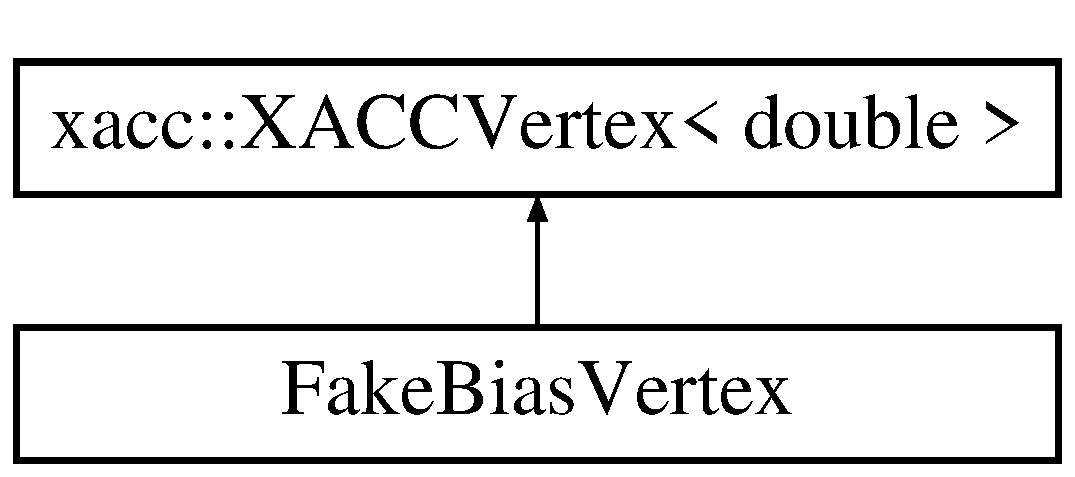
\includegraphics[height=2.000000cm]{a01567}
\end{center}
\end{figure}
\subsection*{Additional Inherited Members}


The documentation for this class was generated from the following file\+:\begin{DoxyCompactItemize}
\item 
Graph\+Tester.\+cpp\end{DoxyCompactItemize}

\hypertarget{a01095}{}\section{xacc\+:\+:quantum\+:\+:Json\+Visitor Class Reference}
\label{a01095}\index{xacc\+::quantum\+::\+Json\+Visitor@{xacc\+::quantum\+::\+Json\+Visitor}}


{\ttfamily \#include $<$Json\+Visitor.\+hpp$>$}

Inheritance diagram for xacc\+:\+:quantum\+:\+:Json\+Visitor\+:\begin{figure}[H]
\begin{center}
\leavevmode
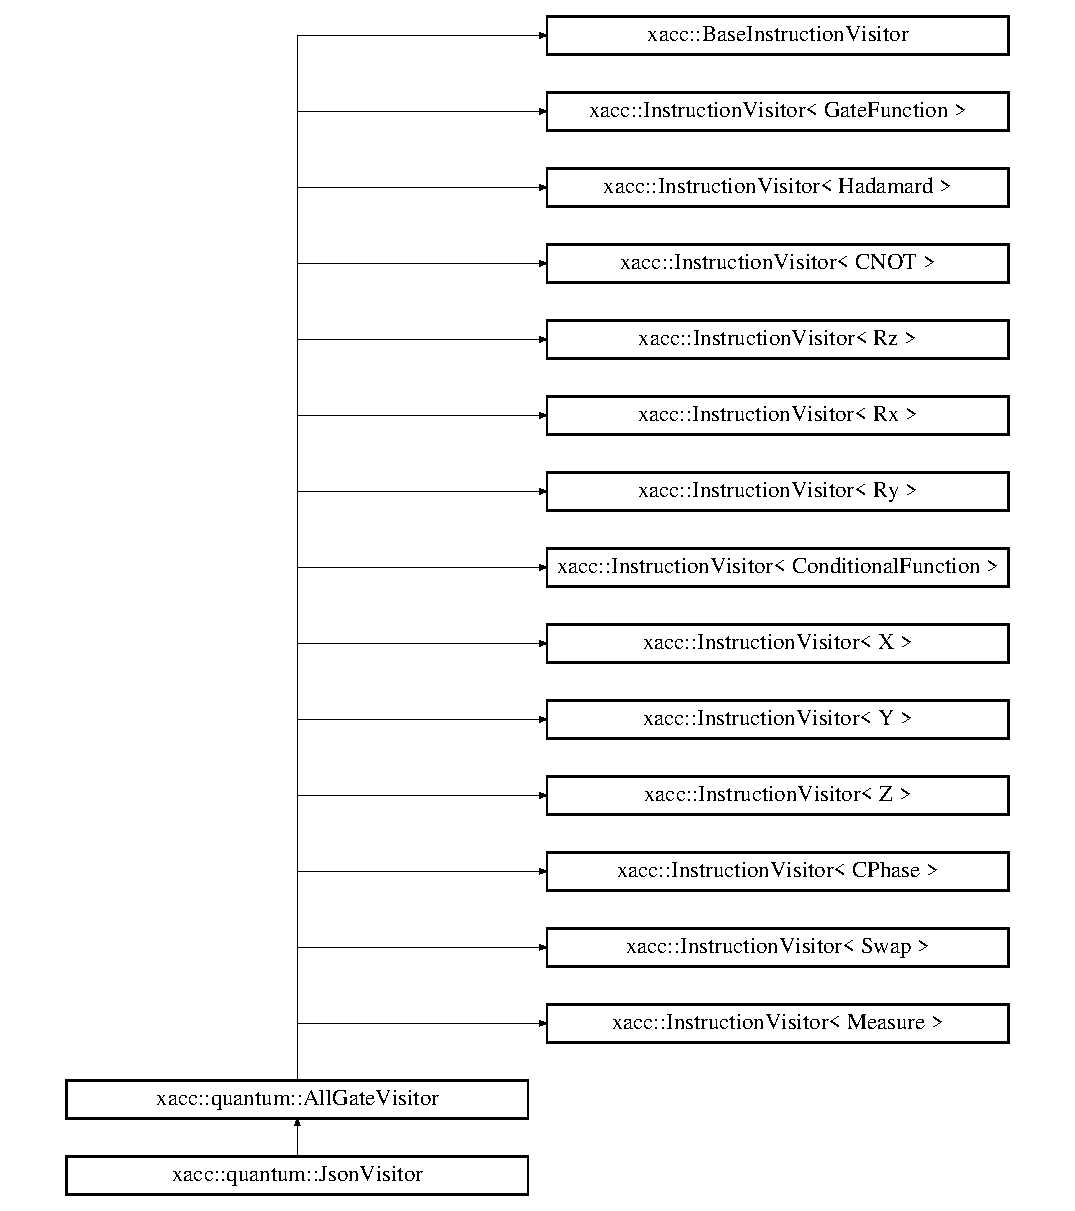
\includegraphics[height=12.000000cm]{a01095}
\end{center}
\end{figure}
\subsection*{Public Member Functions}
\begin{DoxyCompactItemize}
\item 
\mbox{\Hypertarget{a01095_a7b2bf70217828adf6457e3fee7e13056}\label{a01095_a7b2bf70217828adf6457e3fee7e13056}} 
{\bfseries Json\+Visitor} (std\+::shared\+\_\+ptr$<$ \hyperlink{a01151}{xacc\+::\+Function} $>$ f)
\item 
\mbox{\Hypertarget{a01095_a7f2a81b621eaf97f3f7773b566320d02}\label{a01095_a7f2a81b621eaf97f3f7773b566320d02}} 
{\bfseries Json\+Visitor} (std\+::vector$<$ std\+::shared\+\_\+ptr$<$ \hyperlink{a01151}{xacc\+::\+Function} $>$$>$ fs)
\item 
\mbox{\Hypertarget{a01095_a78e2b6c71755a0fed97de43e0b7edc82}\label{a01095_a78e2b6c71755a0fed97de43e0b7edc82}} 
std\+::string {\bfseries write} ()
\item 
\mbox{\Hypertarget{a01095_afdebbabdbae5ecb3a508f02ffe056fd4}\label{a01095_afdebbabdbae5ecb3a508f02ffe056fd4}} 
void {\bfseries visit} (\hyperlink{a01043}{Hadamard} \&h)
\item 
\mbox{\Hypertarget{a01095_a83c17c122c0e02242189b3564290f3e9}\label{a01095_a83c17c122c0e02242189b3564290f3e9}} 
void {\bfseries visit} (\hyperlink{a01031}{C\+N\+OT} \&cn)
\item 
\mbox{\Hypertarget{a01095_afd0b13a59603da5209f84f4b72f77a1a}\label{a01095_afd0b13a59603da5209f84f4b72f77a1a}} 
void {\bfseries visit} (\hyperlink{a01063}{Swap} \&s)
\item 
\mbox{\Hypertarget{a01095_a76c3593f3933631c2dbca74b7b216534}\label{a01095_a76c3593f3933631c2dbca74b7b216534}} 
void {\bfseries visit} (\hyperlink{a01059}{Rz} \&rz)
\item 
\mbox{\Hypertarget{a01095_ad73ac1911e894f315fcee802673a30da}\label{a01095_ad73ac1911e894f315fcee802673a30da}} 
void {\bfseries visit} (\hyperlink{a01051}{Rx} \&rx)
\item 
\mbox{\Hypertarget{a01095_a0e744d9db4c2d16196b17f91a84f8767}\label{a01095_a0e744d9db4c2d16196b17f91a84f8767}} 
void {\bfseries visit} (\hyperlink{a01055}{Ry} \&ry)
\item 
\mbox{\Hypertarget{a01095_aaac9aeecf38aa3e4dae4f43e3884b6d7}\label{a01095_aaac9aeecf38aa3e4dae4f43e3884b6d7}} 
void {\bfseries visit} (\hyperlink{a01039}{C\+Phase} \&cp)
\item 
\mbox{\Hypertarget{a01095_aea63f829d8c926e567ef6a09a0ca779e}\label{a01095_aea63f829d8c926e567ef6a09a0ca779e}} 
void {\bfseries visit} (\hyperlink{a01035}{Conditional\+Function} \&cn)
\item 
\mbox{\Hypertarget{a01095_a71a9c4b78152af3366f8ee93b2e4d9da}\label{a01095_a71a9c4b78152af3366f8ee93b2e4d9da}} 
void {\bfseries visit} (\hyperlink{a01047}{Measure} \&cn)
\item 
\mbox{\Hypertarget{a01095_a2862d01b12da46374c16a3baf33bb4ca}\label{a01095_a2862d01b12da46374c16a3baf33bb4ca}} 
void {\bfseries visit} (\hyperlink{a01067}{X} \&cn)
\item 
\mbox{\Hypertarget{a01095_a5f08b133da5ae583b40d3324220e68e3}\label{a01095_a5f08b133da5ae583b40d3324220e68e3}} 
void {\bfseries visit} (\hyperlink{a01071}{Y} \&y)
\item 
\mbox{\Hypertarget{a01095_a1e1a24feb419b275e2873575242ecbfd}\label{a01095_a1e1a24feb419b275e2873575242ecbfd}} 
void {\bfseries visit} (\hyperlink{a01075}{Z} \&z)
\item 
\mbox{\Hypertarget{a01095_af80f9bd5dda7f53279baa9823c715f60}\label{a01095_af80f9bd5dda7f53279baa9823c715f60}} 
void {\bfseries visit} (\hyperlink{a01011}{Gate\+Function} \&function)
\end{DoxyCompactItemize}
\subsection*{Protected Member Functions}
\begin{DoxyCompactItemize}
\item 
\mbox{\Hypertarget{a01095_adf4795f80bf4773af8babb9ee7d38c96}\label{a01095_adf4795f80bf4773af8babb9ee7d38c96}} 
void {\bfseries base\+Gate\+Inst} (\hyperlink{a01015}{Gate\+Instruction} \&inst, bool end\+Object=true)
\end{DoxyCompactItemize}
\subsection*{Protected Attributes}
\begin{DoxyCompactItemize}
\item 
\mbox{\Hypertarget{a01095_a79e14ac35a004c64f3b6a5c684d73598}\label{a01095_a79e14ac35a004c64f3b6a5c684d73598}} 
std\+::shared\+\_\+ptr$<$ String\+Buffer $>$ {\bfseries buffer}
\item 
\mbox{\Hypertarget{a01095_a4433a92e0c5a1ede71223c275a495241}\label{a01095_a4433a92e0c5a1ede71223c275a495241}} 
std\+::shared\+\_\+ptr$<$ Writer $>$ {\bfseries writer}
\item 
\mbox{\Hypertarget{a01095_ae943110fac6aa057637fbdf76c39ba9c}\label{a01095_ae943110fac6aa057637fbdf76c39ba9c}} 
std\+::shared\+\_\+ptr$<$ \hyperlink{a01151}{Function} $>$ {\bfseries function}
\item 
\mbox{\Hypertarget{a01095_a84ac738710890faa124c0df935bc51d5}\label{a01095_a84ac738710890faa124c0df935bc51d5}} 
std\+::shared\+\_\+ptr$<$ \hyperlink{a01159}{Instruction\+Iterator} $>$ {\bfseries top\+Level\+Instruction\+Iterator}
\item 
\mbox{\Hypertarget{a01095_a3f883a147fed57e8b241a2700f4602d9}\label{a01095_a3f883a147fed57e8b241a2700f4602d9}} 
std\+::vector$<$ std\+::shared\+\_\+ptr$<$ \hyperlink{a01151}{Function} $>$ $>$ {\bfseries functions}
\end{DoxyCompactItemize}


\subsection{Detailed Description}
F\+I\+X\+ME write this 

The documentation for this class was generated from the following file\+:\begin{DoxyCompactItemize}
\item 
Json\+Visitor.\+hpp\end{DoxyCompactItemize}

\hypertarget{a01563}{}\section{Fake\+Tensor\+Vertex Class Reference}
\label{a01563}\index{Fake\+Tensor\+Vertex@{Fake\+Tensor\+Vertex}}
Inheritance diagram for Fake\+Tensor\+Vertex\+:\begin{figure}[H]
\begin{center}
\leavevmode
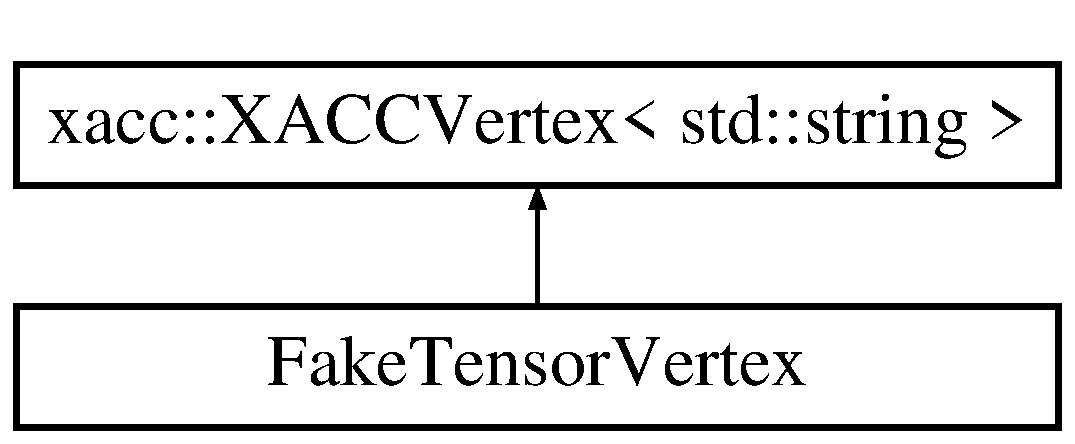
\includegraphics[height=2.000000cm]{a01563}
\end{center}
\end{figure}
\subsection*{Additional Inherited Members}


The documentation for this class was generated from the following file\+:\begin{DoxyCompactItemize}
\item 
Graph\+Tester.\+cpp\end{DoxyCompactItemize}

\hypertarget{a01571}{}\section{Fake\+Vertex\+Four\+Properties Class Reference}
\label{a01571}\index{Fake\+Vertex\+Four\+Properties@{Fake\+Vertex\+Four\+Properties}}
Inheritance diagram for Fake\+Vertex\+Four\+Properties\+:\begin{figure}[H]
\begin{center}
\leavevmode
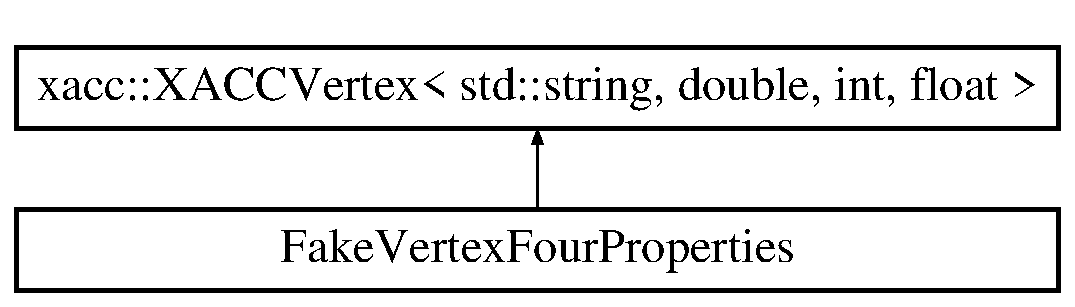
\includegraphics[height=2.000000cm]{a01571}
\end{center}
\end{figure}
\subsection*{Additional Inherited Members}


The documentation for this class was generated from the following file\+:\begin{DoxyCompactItemize}
\item 
Graph\+Tester.\+cpp\end{DoxyCompactItemize}

\hypertarget{a01575}{}\section{Fake\+Vertex\+Four\+Properties\+Print2 Class Reference}
\label{a01575}\index{Fake\+Vertex\+Four\+Properties\+Print2@{Fake\+Vertex\+Four\+Properties\+Print2}}
Inheritance diagram for Fake\+Vertex\+Four\+Properties\+Print2\+:\begin{figure}[H]
\begin{center}
\leavevmode
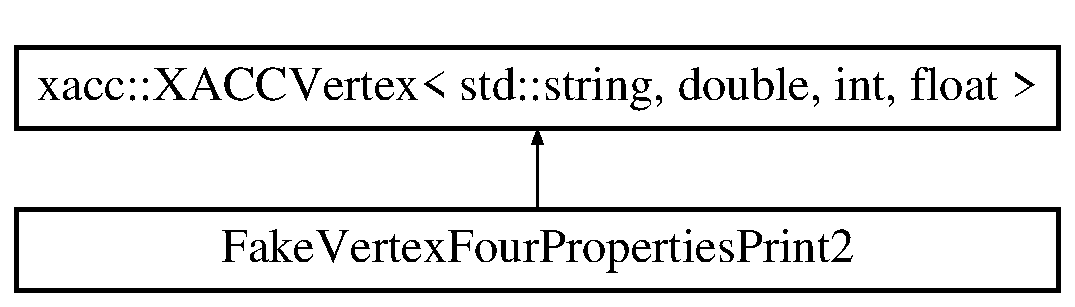
\includegraphics[height=2.000000cm]{a01575}
\end{center}
\end{figure}
\subsection*{Additional Inherited Members}


The documentation for this class was generated from the following file\+:\begin{DoxyCompactItemize}
\item 
Graph\+Tester.\+cpp\end{DoxyCompactItemize}

\hypertarget{a01579}{}\section{Fake\+Vertex\+With\+Vector Class Reference}
\label{a01579}\index{Fake\+Vertex\+With\+Vector@{Fake\+Vertex\+With\+Vector}}
Inheritance diagram for Fake\+Vertex\+With\+Vector\+:\begin{figure}[H]
\begin{center}
\leavevmode
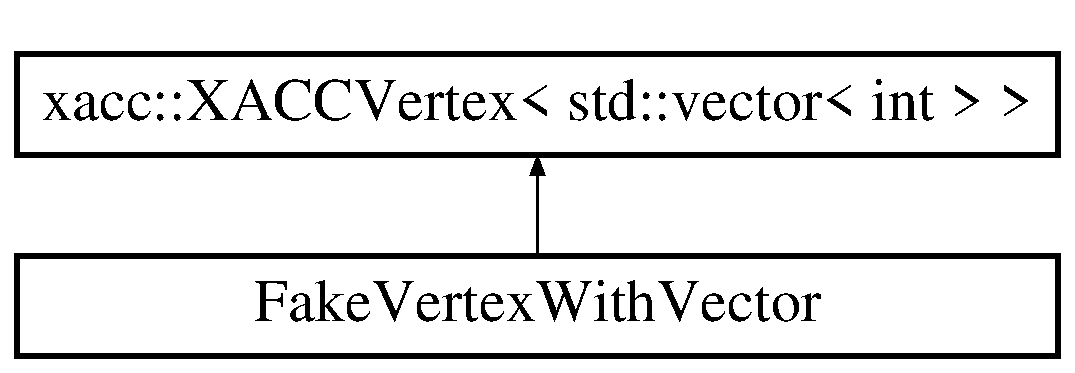
\includegraphics[height=2.000000cm]{a01579}
\end{center}
\end{figure}
\subsection*{Additional Inherited Members}


The documentation for this class was generated from the following file\+:\begin{DoxyCompactItemize}
\item 
Graph\+Tester.\+cpp\end{DoxyCompactItemize}

\hypertarget{a01319}{}\section{File\+Generator Struct Reference}
\label{a01319}\index{File\+Generator@{File\+Generator}}


The documentation for this struct was generated from the following file\+:\begin{DoxyCompactItemize}
\item 
Delimited\+Text\+Parser\+Test.\+cpp\end{DoxyCompactItemize}

\hypertarget{a01403}{}\section{C\+Simple\+Ini\+Templ$<$ S\+I\+\_\+\+C\+H\+AR, S\+I\+\_\+\+S\+T\+R\+L\+E\+SS, S\+I\+\_\+\+C\+O\+N\+V\+E\+R\+T\+ER $>$\+:\+:File\+Writer Class Reference}
\label{a01403}\index{C\+Simple\+Ini\+Templ$<$ S\+I\+\_\+\+C\+H\+A\+R, S\+I\+\_\+\+S\+T\+R\+L\+E\+S\+S, S\+I\+\_\+\+C\+O\+N\+V\+E\+R\+T\+E\+R $>$\+::\+File\+Writer@{C\+Simple\+Ini\+Templ$<$ S\+I\+\_\+\+C\+H\+A\+R, S\+I\+\_\+\+S\+T\+R\+L\+E\+S\+S, S\+I\+\_\+\+C\+O\+N\+V\+E\+R\+T\+E\+R $>$\+::\+File\+Writer}}


{\ttfamily \#include $<$Simple\+Ini.\+h$>$}

Inheritance diagram for C\+Simple\+Ini\+Templ$<$ S\+I\+\_\+\+C\+H\+AR, S\+I\+\_\+\+S\+T\+R\+L\+E\+SS, S\+I\+\_\+\+C\+O\+N\+V\+E\+R\+T\+ER $>$\+:\+:File\+Writer\+:\begin{figure}[H]
\begin{center}
\leavevmode
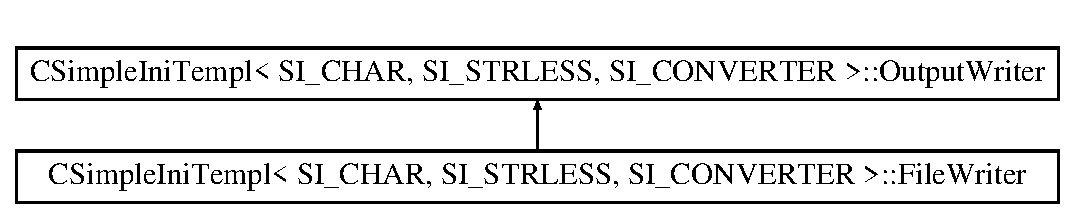
\includegraphics[height=2.000000cm]{a01403}
\end{center}
\end{figure}
\subsection*{Public Member Functions}
\begin{DoxyCompactItemize}
\item 
\mbox{\Hypertarget{a01403_aecd4d79480c9b4e70b598c10014856f8}\label{a01403_aecd4d79480c9b4e70b598c10014856f8}} 
{\bfseries File\+Writer} (F\+I\+LE $\ast$a\+\_\+file)
\item 
\mbox{\Hypertarget{a01403_ae8885b97884ef9dd5bf074bc4f011373}\label{a01403_ae8885b97884ef9dd5bf074bc4f011373}} 
void {\bfseries Write} (const char $\ast$a\+\_\+p\+Buf)
\end{DoxyCompactItemize}


\subsection{Detailed Description}
\subsubsection*{template$<$class S\+I\+\_\+\+C\+H\+AR, class S\+I\+\_\+\+S\+T\+R\+L\+E\+SS, class S\+I\+\_\+\+C\+O\+N\+V\+E\+R\+T\+ER$>$\newline
class C\+Simple\+Ini\+Templ$<$ S\+I\+\_\+\+C\+H\+A\+R, S\+I\+\_\+\+S\+T\+R\+L\+E\+S\+S, S\+I\+\_\+\+C\+O\+N\+V\+E\+R\+T\+E\+R $>$\+::\+File\+Writer}

\hyperlink{a01399}{Output\+Writer} class to write the I\+NI data to a file 

The documentation for this class was generated from the following file\+:\begin{DoxyCompactItemize}
\item 
Simple\+Ini.\+h\end{DoxyCompactItemize}

\hypertarget{a01327}{}\section{foo Class Reference}
\label{a01327}\index{foo@{foo}}


{\ttfamily \#include $<$O\+D\+E\+Solver.\+h$>$}



\subsection{Detailed Description}


 Copyright (c) 2015-\/, U\+T-\/\+Battelle, L\+LC All rights reserved.

Redistribution and use in source and binary forms, with or without modification, are permitted provided that the following conditions are met\+:

Redistributions of source code must retain the above copyright notice, this list of conditions and the following disclaimer.

Redistributions in binary form must reproduce the above copyright notice, this list of conditions and the following disclaimer in the documentation and/or other materials provided with the distribution.

Neither the name of fern nor the names of its contributors may be used to endorse or promote products derived from this software without specific prior written permission.

T\+H\+IS S\+O\+F\+T\+W\+A\+RE IS P\+R\+O\+V\+I\+D\+ED BY T\+HE C\+O\+P\+Y\+R\+I\+G\+HT H\+O\+L\+D\+E\+RS A\+ND C\+O\+N\+T\+R\+I\+B\+U\+T\+O\+RS \char`\"{}\+A\+S I\+S\char`\"{} A\+ND A\+NY E\+X\+P\+R\+E\+SS OR I\+M\+P\+L\+I\+ED W\+A\+R\+R\+A\+N\+T\+I\+ES, I\+N\+C\+L\+U\+D\+I\+NG, B\+UT N\+OT L\+I\+M\+I\+T\+ED TO, T\+HE I\+M\+P\+L\+I\+ED W\+A\+R\+R\+A\+N\+T\+I\+ES OF M\+E\+R\+C\+H\+A\+N\+T\+A\+B\+I\+L\+I\+TY A\+ND F\+I\+T\+N\+E\+SS F\+OR A P\+A\+R\+T\+I\+C\+U\+L\+AR P\+U\+R\+P\+O\+SE A\+RE D\+I\+S\+C\+L\+A\+I\+M\+ED. IN NO E\+V\+E\+NT S\+H\+A\+LL T\+HE C\+O\+P\+Y\+R\+I\+G\+HT H\+O\+L\+D\+ER OR C\+O\+N\+T\+R\+I\+B\+U\+T\+O\+RS BE L\+I\+A\+B\+LE F\+OR A\+NY D\+I\+R\+E\+CT, I\+N\+D\+I\+R\+E\+CT, I\+N\+C\+I\+D\+E\+N\+T\+AL, S\+P\+E\+C\+I\+AL, E\+X\+E\+M\+P\+L\+A\+RY, OR C\+O\+N\+S\+E\+Q\+U\+E\+N\+T\+I\+AL D\+A\+M\+A\+G\+ES (I\+N\+C\+L\+U\+D\+I\+NG, B\+UT N\+OT L\+I\+M\+I\+T\+ED TO, P\+R\+O\+C\+U\+R\+E\+M\+E\+NT OF S\+U\+B\+S\+T\+I\+T\+U\+TE G\+O\+O\+DS OR S\+E\+R\+V\+I\+C\+ES; L\+O\+SS OF U\+SE, D\+A\+TA, OR P\+R\+O\+F\+I\+TS; OR B\+U\+S\+I\+N\+E\+SS I\+N\+T\+E\+R\+R\+U\+P\+T\+I\+ON) H\+O\+W\+E\+V\+ER C\+A\+U\+S\+ED A\+ND ON A\+NY T\+H\+E\+O\+RY OF L\+I\+A\+B\+I\+L\+I\+TY, W\+H\+E\+T\+H\+ER IN C\+O\+N\+T\+R\+A\+CT, S\+T\+R\+I\+CT L\+I\+A\+B\+I\+L\+I\+TY, OR T\+O\+RT (I\+N\+C\+L\+U\+D\+I\+NG N\+E\+G\+L\+I\+G\+E\+N\+CE OR O\+T\+H\+E\+R\+W\+I\+SE) A\+R\+I\+S\+I\+NG IN A\+NY W\+AY O\+UT OF T\+HE U\+SE OF T\+H\+IS S\+O\+F\+T\+W\+A\+RE, E\+V\+EN IF A\+D\+V\+I\+S\+ED OF T\+HE P\+O\+S\+S\+I\+B\+I\+L\+I\+TY OF S\+U\+CH D\+A\+M\+A\+GE.

\subsubsection*{Author(s)\+: Jay Jay Billings (jayjaybillings  gmail  com) }

The documentation for this class was generated from the following file\+:\begin{DoxyCompactItemize}
\item 
O\+D\+E\+Solver.\+h\end{DoxyCompactItemize}

\hypertarget{a01475}{}\section{xacc\+:\+:Function Class Reference}
\label{a01475}\index{xacc\+::\+Function@{xacc\+::\+Function}}


{\ttfamily \#include $<$Function.\+hpp$>$}

Inheritance diagram for xacc\+:\+:Function\+:\begin{figure}[H]
\begin{center}
\leavevmode
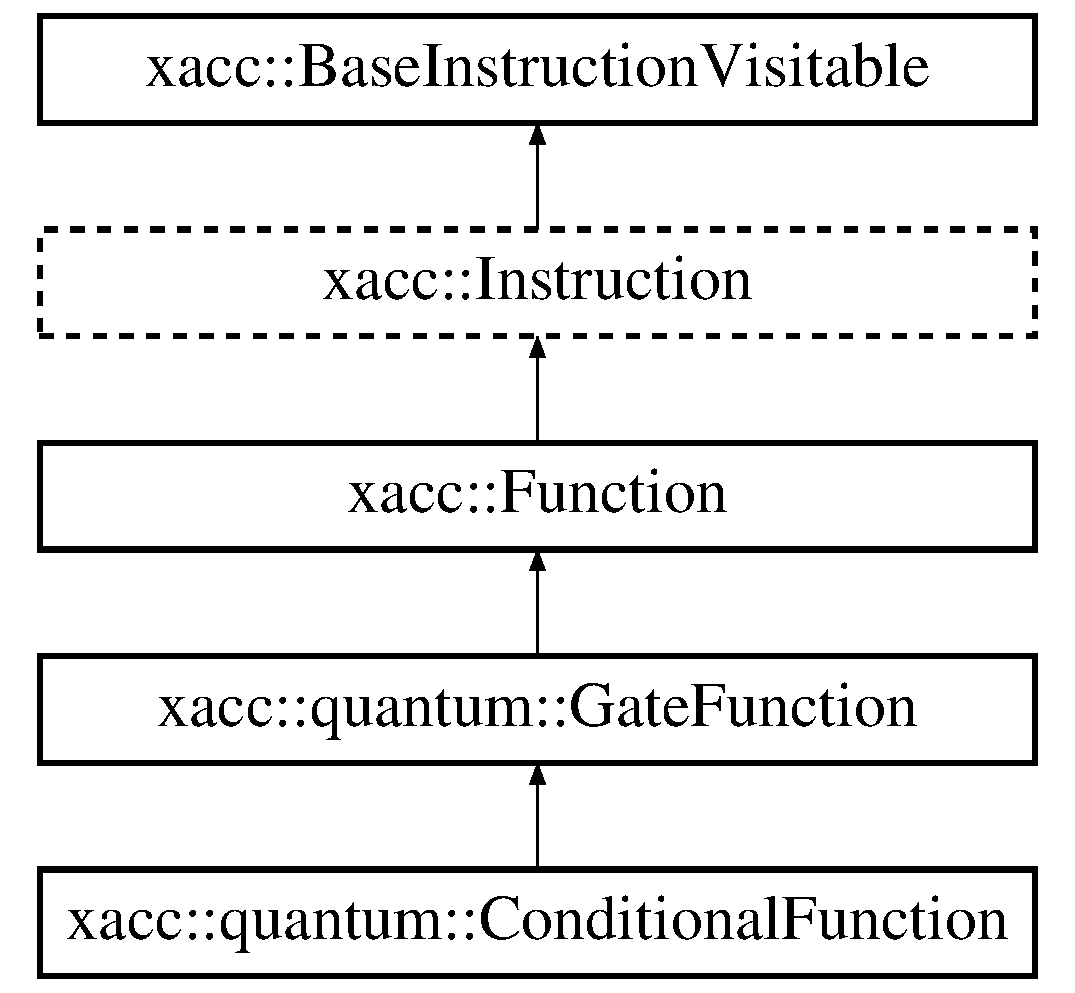
\includegraphics[height=5.000000cm]{a01475}
\end{center}
\end{figure}
\subsection*{Public Member Functions}
\begin{DoxyCompactItemize}
\item 
virtual const int \hyperlink{a01475_a8901985525f59713e14c61713e07c086}{n\+Instructions} ()=0
\item 
virtual Inst\+Ptr \hyperlink{a01475_afa549fc91b5a05f26d8139954a7e0ed5}{get\+Instruction} (const int idx)=0
\item 
virtual std\+::list$<$ Inst\+Ptr $>$ \hyperlink{a01475_aaf80bd3d49113a92b520785572663032}{get\+Instructions} ()=0
\item 
virtual void \hyperlink{a01475_ab6478b09bb28e194bb555b3180737733}{remove\+Instruction} (const int idx)=0
\item 
virtual void \hyperlink{a01475_a2ef6a4923a6734f90f6ee3d94d263af0}{replace\+Instruction} (const int idx, Inst\+Ptr new\+Inst)=0
\item 
virtual void \hyperlink{a01475_acde702e44bdbc2759b338365218d7ebe}{insert\+Instruction} (const int idx, Inst\+Ptr new\+Inst)=0
\item 
virtual void \hyperlink{a01475_aa8c9ec2d08be75c69399d4254b0216f5}{add\+Instruction} (Inst\+Ptr instruction)=0
\item 
virtual bool \hyperlink{a01475_aa75500c657b5c3e0e36213e1506aad97}{is\+Composite} ()
\item 
virtual void \hyperlink{a01475_af6ae9453027789a2aaec30e59c9e45e3}{evaluate\+Variable\+Parameters} (std\+::vector$<$ Instruction\+Parameter $>$ parameters)=0
\item 
virtual \hyperlink{a01475_a04b25ba4da1ddfa4ec4ec6d6ffb25bc3}{$\sim$\+Function} ()
\end{DoxyCompactItemize}
\subsection*{Additional Inherited Members}


\subsection{Detailed Description}
The \hyperlink{a01475}{Function} is an \hyperlink{a01479}{Instruction} that contains further child Instructions.

\begin{DoxyAuthor}{Author}
Alex Mc\+Caskey 
\end{DoxyAuthor}


\subsection{Constructor \& Destructor Documentation}
\mbox{\Hypertarget{a01475_a04b25ba4da1ddfa4ec4ec6d6ffb25bc3}\label{a01475_a04b25ba4da1ddfa4ec4ec6d6ffb25bc3}} 
\index{xacc\+::\+Function@{xacc\+::\+Function}!````~Function@{$\sim$\+Function}}
\index{````~Function@{$\sim$\+Function}!xacc\+::\+Function@{xacc\+::\+Function}}
\subsubsection{\texorpdfstring{$\sim$\+Function()}{~Function()}}
{\footnotesize\ttfamily virtual xacc\+::\+Function\+::$\sim$\+Function (\begin{DoxyParamCaption}{ }\end{DoxyParamCaption})\hspace{0.3cm}{\ttfamily [inline]}, {\ttfamily [virtual]}}

The destructor 

\subsection{Member Function Documentation}
\mbox{\Hypertarget{a01475_aa8c9ec2d08be75c69399d4254b0216f5}\label{a01475_aa8c9ec2d08be75c69399d4254b0216f5}} 
\index{xacc\+::\+Function@{xacc\+::\+Function}!add\+Instruction@{add\+Instruction}}
\index{add\+Instruction@{add\+Instruction}!xacc\+::\+Function@{xacc\+::\+Function}}
\subsubsection{\texorpdfstring{add\+Instruction()}{addInstruction()}}
{\footnotesize\ttfamily virtual void xacc\+::\+Function\+::add\+Instruction (\begin{DoxyParamCaption}\item[{Inst\+Ptr}]{instruction }\end{DoxyParamCaption})\hspace{0.3cm}{\ttfamily [pure virtual]}}

Add an \hyperlink{a01479}{Instruction} to this \hyperlink{a01475}{Function}.


\begin{DoxyParams}{Parameters}
{\em instruction} & The instruction to add. \\
\hline
\end{DoxyParams}


Implemented in \hyperlink{a01155_a892fb69a10f0a7cb5abdab4cca61b80a}{xacc\+::quantum\+::\+Gate\+Function}, and \hyperlink{a01179_a6aedad20f96390880efdc0a476b3273f}{xacc\+::quantum\+::\+Conditional\+Function}.

\mbox{\Hypertarget{a01475_af6ae9453027789a2aaec30e59c9e45e3}\label{a01475_af6ae9453027789a2aaec30e59c9e45e3}} 
\index{xacc\+::\+Function@{xacc\+::\+Function}!evaluate\+Variable\+Parameters@{evaluate\+Variable\+Parameters}}
\index{evaluate\+Variable\+Parameters@{evaluate\+Variable\+Parameters}!xacc\+::\+Function@{xacc\+::\+Function}}
\subsubsection{\texorpdfstring{evaluate\+Variable\+Parameters()}{evaluateVariableParameters()}}
{\footnotesize\ttfamily virtual void xacc\+::\+Function\+::evaluate\+Variable\+Parameters (\begin{DoxyParamCaption}\item[{std\+::vector$<$ Instruction\+Parameter $>$}]{parameters }\end{DoxyParamCaption})\hspace{0.3cm}{\ttfamily [pure virtual]}}

This method is used to evaluate this \hyperlink{a01475}{Function}\textquotesingle{}s parameterized Instructions that have string variable Instruction\+Parameters. These parameters are updated with the given runtime parameters.


\begin{DoxyParams}{Parameters}
{\em parameters} & The runtime parameters \\
\hline
\end{DoxyParams}


Implemented in \hyperlink{a01155_a4bcbd2c8c4b615d74e4a4d39952fd411}{xacc\+::quantum\+::\+Gate\+Function}.

\mbox{\Hypertarget{a01475_afa549fc91b5a05f26d8139954a7e0ed5}\label{a01475_afa549fc91b5a05f26d8139954a7e0ed5}} 
\index{xacc\+::\+Function@{xacc\+::\+Function}!get\+Instruction@{get\+Instruction}}
\index{get\+Instruction@{get\+Instruction}!xacc\+::\+Function@{xacc\+::\+Function}}
\subsubsection{\texorpdfstring{get\+Instruction()}{getInstruction()}}
{\footnotesize\ttfamily virtual Inst\+Ptr xacc\+::\+Function\+::get\+Instruction (\begin{DoxyParamCaption}\item[{const int}]{idx }\end{DoxyParamCaption})\hspace{0.3cm}{\ttfamily [pure virtual]}}

Return the \hyperlink{a01479}{Instruction} at the given index.


\begin{DoxyParams}{Parameters}
{\em idx} & The desired \hyperlink{a01479}{Instruction} index \\
\hline
\end{DoxyParams}
\begin{DoxyReturn}{Returns}
inst The instruction at the given index. 
\end{DoxyReturn}


Implemented in \hyperlink{a01155_a841d656eed8aa9b4c0eec3f1da38069c}{xacc\+::quantum\+::\+Gate\+Function}.

\mbox{\Hypertarget{a01475_aaf80bd3d49113a92b520785572663032}\label{a01475_aaf80bd3d49113a92b520785572663032}} 
\index{xacc\+::\+Function@{xacc\+::\+Function}!get\+Instructions@{get\+Instructions}}
\index{get\+Instructions@{get\+Instructions}!xacc\+::\+Function@{xacc\+::\+Function}}
\subsubsection{\texorpdfstring{get\+Instructions()}{getInstructions()}}
{\footnotesize\ttfamily virtual std\+::list$<$Inst\+Ptr$>$ xacc\+::\+Function\+::get\+Instructions (\begin{DoxyParamCaption}{ }\end{DoxyParamCaption})\hspace{0.3cm}{\ttfamily [pure virtual]}}

Return all Instructions in this \hyperlink{a01475}{Function}

\begin{DoxyReturn}{Returns}
insts The list of this \hyperlink{a01475}{Function}\textquotesingle{}s Instructions 
\end{DoxyReturn}


Implemented in \hyperlink{a01155_aebce6a9e64aed7f4aff86df752bacfe2}{xacc\+::quantum\+::\+Gate\+Function}.

\mbox{\Hypertarget{a01475_acde702e44bdbc2759b338365218d7ebe}\label{a01475_acde702e44bdbc2759b338365218d7ebe}} 
\index{xacc\+::\+Function@{xacc\+::\+Function}!insert\+Instruction@{insert\+Instruction}}
\index{insert\+Instruction@{insert\+Instruction}!xacc\+::\+Function@{xacc\+::\+Function}}
\subsubsection{\texorpdfstring{insert\+Instruction()}{insertInstruction()}}
{\footnotesize\ttfamily virtual void xacc\+::\+Function\+::insert\+Instruction (\begin{DoxyParamCaption}\item[{const int}]{idx,  }\item[{Inst\+Ptr}]{new\+Inst }\end{DoxyParamCaption})\hspace{0.3cm}{\ttfamily [pure virtual]}}

Insert a new \hyperlink{a01479}{Instruction} at the given index. All previous instructions are pushed back, ie their new indices are current\+Index + 1.


\begin{DoxyParams}{Parameters}
{\em idx} & The index where the new instruction should be inserted \\
\hline
{\em new\+Inst} & The new \hyperlink{a01479}{Instruction} to insert. \\
\hline
\end{DoxyParams}


Implemented in \hyperlink{a01155_aed3b963f1c4eb3215ca46af48d78f588}{xacc\+::quantum\+::\+Gate\+Function}.

\mbox{\Hypertarget{a01475_aa75500c657b5c3e0e36213e1506aad97}\label{a01475_aa75500c657b5c3e0e36213e1506aad97}} 
\index{xacc\+::\+Function@{xacc\+::\+Function}!is\+Composite@{is\+Composite}}
\index{is\+Composite@{is\+Composite}!xacc\+::\+Function@{xacc\+::\+Function}}
\subsubsection{\texorpdfstring{is\+Composite()}{isComposite()}}
{\footnotesize\ttfamily virtual bool xacc\+::\+Function\+::is\+Composite (\begin{DoxyParamCaption}{ }\end{DoxyParamCaption})\hspace{0.3cm}{\ttfamily [inline]}, {\ttfamily [virtual]}}

Return true always to indicate that the \hyperlink{a01475}{Function} is composite.

\begin{DoxyReturn}{Returns}
composite True indicating this is a composite \hyperlink{a01479}{Instruction}. 
\end{DoxyReturn}


Reimplemented from \hyperlink{a01479_a4383f1036d0fcfe890ab9c613dbd5f38}{xacc\+::\+Instruction}.

\mbox{\Hypertarget{a01475_a8901985525f59713e14c61713e07c086}\label{a01475_a8901985525f59713e14c61713e07c086}} 
\index{xacc\+::\+Function@{xacc\+::\+Function}!n\+Instructions@{n\+Instructions}}
\index{n\+Instructions@{n\+Instructions}!xacc\+::\+Function@{xacc\+::\+Function}}
\subsubsection{\texorpdfstring{n\+Instructions()}{nInstructions()}}
{\footnotesize\ttfamily virtual const int xacc\+::\+Function\+::n\+Instructions (\begin{DoxyParamCaption}{ }\end{DoxyParamCaption})\hspace{0.3cm}{\ttfamily [pure virtual]}}

Return the number of Instructions that this \hyperlink{a01475}{Function} contains.

\begin{DoxyReturn}{Returns}
n\+Inst The number of instructions 
\end{DoxyReturn}


Implemented in \hyperlink{a01155_aa70b26156c060fec71316fe5e98bb102}{xacc\+::quantum\+::\+Gate\+Function}.

\mbox{\Hypertarget{a01475_ab6478b09bb28e194bb555b3180737733}\label{a01475_ab6478b09bb28e194bb555b3180737733}} 
\index{xacc\+::\+Function@{xacc\+::\+Function}!remove\+Instruction@{remove\+Instruction}}
\index{remove\+Instruction@{remove\+Instruction}!xacc\+::\+Function@{xacc\+::\+Function}}
\subsubsection{\texorpdfstring{remove\+Instruction()}{removeInstruction()}}
{\footnotesize\ttfamily virtual void xacc\+::\+Function\+::remove\+Instruction (\begin{DoxyParamCaption}\item[{const int}]{idx }\end{DoxyParamCaption})\hspace{0.3cm}{\ttfamily [pure virtual]}}

Remove the \hyperlink{a01479}{Instruction} at the given index.


\begin{DoxyParams}{Parameters}
{\em idx} & The index of the \hyperlink{a01479}{Instruction} to remove. \\
\hline
\end{DoxyParams}


Implemented in \hyperlink{a01155_a44ca35d081577de9ad2930f93c01e89d}{xacc\+::quantum\+::\+Gate\+Function}.

\mbox{\Hypertarget{a01475_a2ef6a4923a6734f90f6ee3d94d263af0}\label{a01475_a2ef6a4923a6734f90f6ee3d94d263af0}} 
\index{xacc\+::\+Function@{xacc\+::\+Function}!replace\+Instruction@{replace\+Instruction}}
\index{replace\+Instruction@{replace\+Instruction}!xacc\+::\+Function@{xacc\+::\+Function}}
\subsubsection{\texorpdfstring{replace\+Instruction()}{replaceInstruction()}}
{\footnotesize\ttfamily virtual void xacc\+::\+Function\+::replace\+Instruction (\begin{DoxyParamCaption}\item[{const int}]{idx,  }\item[{Inst\+Ptr}]{new\+Inst }\end{DoxyParamCaption})\hspace{0.3cm}{\ttfamily [pure virtual]}}

Replace the \hyperlink{a01479}{Instruction} at the given index with the given new \hyperlink{a01479}{Instruction}.


\begin{DoxyParams}{Parameters}
{\em idx} & The index of the \hyperlink{a01479}{Instruction} to replace. \\
\hline
{\em new\+Inst} & The new \hyperlink{a01479}{Instruction} to replace with. \\
\hline
\end{DoxyParams}


Implemented in \hyperlink{a01155_a182fdfabbf546ae89e4f2384bafb45c9}{xacc\+::quantum\+::\+Gate\+Function}.



The documentation for this class was generated from the following file\+:\begin{DoxyCompactItemize}
\item 
Function.\+hpp\end{DoxyCompactItemize}

\hypertarget{a01231}{}\section{xacc\+:\+:Singleton$<$ T $>$ Class Template Reference}
\label{a01231}\index{xacc\+::\+Singleton$<$ T $>$@{xacc\+::\+Singleton$<$ T $>$}}


{\ttfamily \#include $<$Singleton.\+hpp$>$}

\subsection*{Static Public Member Functions}
\begin{DoxyCompactItemize}
\item 
static T $\ast$ \hyperlink{a01231_ae4c30f303439e702389c9d088abb3f23}{instance} ()
\item 
static void \hyperlink{a01231_abbc654f5f90a2abc85f0010496335942}{destroy} ()
\end{DoxyCompactItemize}
\subsection*{Protected Member Functions}
\begin{DoxyCompactItemize}
\item 
\hyperlink{a01231_afd62caabc41babdd98ab9af2253ec371}{Singleton} ()
\item 
virtual \hyperlink{a01231_a75a032ec71f88d6986461b47f3fb2600}{$\sim$\+Singleton} ()
\end{DoxyCompactItemize}
\subsection*{Static Protected Attributes}
\begin{DoxyCompactItemize}
\item 
static T $\ast$ \hyperlink{a01231_a863885efab9990f06f699567648dfa26}{instance\+\_\+} = nullptr
\end{DoxyCompactItemize}


\subsection{Detailed Description}
\subsubsection*{template$<$class T$>$\newline
class xacc\+::\+Singleton$<$ T $>$}

\hyperlink{a01231}{Singleton} provides a templated implementation of the \hyperlink{a01231}{Singleton} Design Pattern. This class takes a template parameter and provides behviour around that template that models a singleton -\/ ie there is only one instance available during runtime. 

\subsection{Constructor \& Destructor Documentation}
\mbox{\Hypertarget{a01231_afd62caabc41babdd98ab9af2253ec371}\label{a01231_afd62caabc41babdd98ab9af2253ec371}} 
\index{xacc\+::\+Singleton@{xacc\+::\+Singleton}!Singleton@{Singleton}}
\index{Singleton@{Singleton}!xacc\+::\+Singleton@{xacc\+::\+Singleton}}
\subsubsection{\texorpdfstring{Singleton()}{Singleton()}}
{\footnotesize\ttfamily template$<$class T$>$ \\
\hyperlink{a01231}{xacc\+::\+Singleton}$<$ T $>$\+::\hyperlink{a01231}{Singleton} (\begin{DoxyParamCaption}{ }\end{DoxyParamCaption})\hspace{0.3cm}{\ttfamily [inline]}, {\ttfamily [explicit]}, {\ttfamily [protected]}}

constructor \mbox{\Hypertarget{a01231_a75a032ec71f88d6986461b47f3fb2600}\label{a01231_a75a032ec71f88d6986461b47f3fb2600}} 
\index{xacc\+::\+Singleton@{xacc\+::\+Singleton}!````~Singleton@{$\sim$\+Singleton}}
\index{````~Singleton@{$\sim$\+Singleton}!xacc\+::\+Singleton@{xacc\+::\+Singleton}}
\subsubsection{\texorpdfstring{$\sim$\+Singleton()}{~Singleton()}}
{\footnotesize\ttfamily template$<$class T$>$ \\
virtual \hyperlink{a01231}{xacc\+::\+Singleton}$<$ T $>$\+::$\sim$\hyperlink{a01231}{Singleton} (\begin{DoxyParamCaption}{ }\end{DoxyParamCaption})\hspace{0.3cm}{\ttfamily [inline]}, {\ttfamily [protected]}, {\ttfamily [virtual]}}

destructor 

\subsection{Member Function Documentation}
\mbox{\Hypertarget{a01231_abbc654f5f90a2abc85f0010496335942}\label{a01231_abbc654f5f90a2abc85f0010496335942}} 
\index{xacc\+::\+Singleton@{xacc\+::\+Singleton}!destroy@{destroy}}
\index{destroy@{destroy}!xacc\+::\+Singleton@{xacc\+::\+Singleton}}
\subsubsection{\texorpdfstring{destroy()}{destroy()}}
{\footnotesize\ttfamily template$<$class T$>$ \\
static void \hyperlink{a01231}{xacc\+::\+Singleton}$<$ T $>$\+::destroy (\begin{DoxyParamCaption}{ }\end{DoxyParamCaption})\hspace{0.3cm}{\ttfamily [inline]}, {\ttfamily [static]}}

Destroy the single instance of T \mbox{\Hypertarget{a01231_ae4c30f303439e702389c9d088abb3f23}\label{a01231_ae4c30f303439e702389c9d088abb3f23}} 
\index{xacc\+::\+Singleton@{xacc\+::\+Singleton}!instance@{instance}}
\index{instance@{instance}!xacc\+::\+Singleton@{xacc\+::\+Singleton}}
\subsubsection{\texorpdfstring{instance()}{instance()}}
{\footnotesize\ttfamily template$<$class T$>$ \\
static T$\ast$ \hyperlink{a01231}{xacc\+::\+Singleton}$<$ T $>$\+::instance (\begin{DoxyParamCaption}{ }\end{DoxyParamCaption})\hspace{0.3cm}{\ttfamily [inline]}, {\ttfamily [static]}}

Return the single instance of T \begin{DoxyReturn}{Returns}
instance The singleton instance 
\end{DoxyReturn}


\subsection{Member Data Documentation}
\mbox{\Hypertarget{a01231_a863885efab9990f06f699567648dfa26}\label{a01231_a863885efab9990f06f699567648dfa26}} 
\index{xacc\+::\+Singleton@{xacc\+::\+Singleton}!instance\+\_\+@{instance\+\_\+}}
\index{instance\+\_\+@{instance\+\_\+}!xacc\+::\+Singleton@{xacc\+::\+Singleton}}
\subsubsection{\texorpdfstring{instance\+\_\+}{instance\_}}
{\footnotesize\ttfamily template$<$class T$>$ \\
T $\ast$ \hyperlink{a01231}{xacc\+::\+Singleton}$<$ T $>$\+::instance\+\_\+ = nullptr\hspace{0.3cm}{\ttfamily [static]}, {\ttfamily [protected]}}

Reference to the single T instance 

The documentation for this class was generated from the following file\+:\begin{DoxyCompactItemize}
\item 
Singleton.\+hpp\end{DoxyCompactItemize}

\hypertarget{a01155}{}\section{xacc\+:\+:Instruction Class Reference}
\label{a01155}\index{xacc\+::\+Instruction@{xacc\+::\+Instruction}}


{\ttfamily \#include $<$Instruction.\+hpp$>$}

Inheritance diagram for xacc\+:\+:Instruction\+:\begin{figure}[H]
\begin{center}
\leavevmode
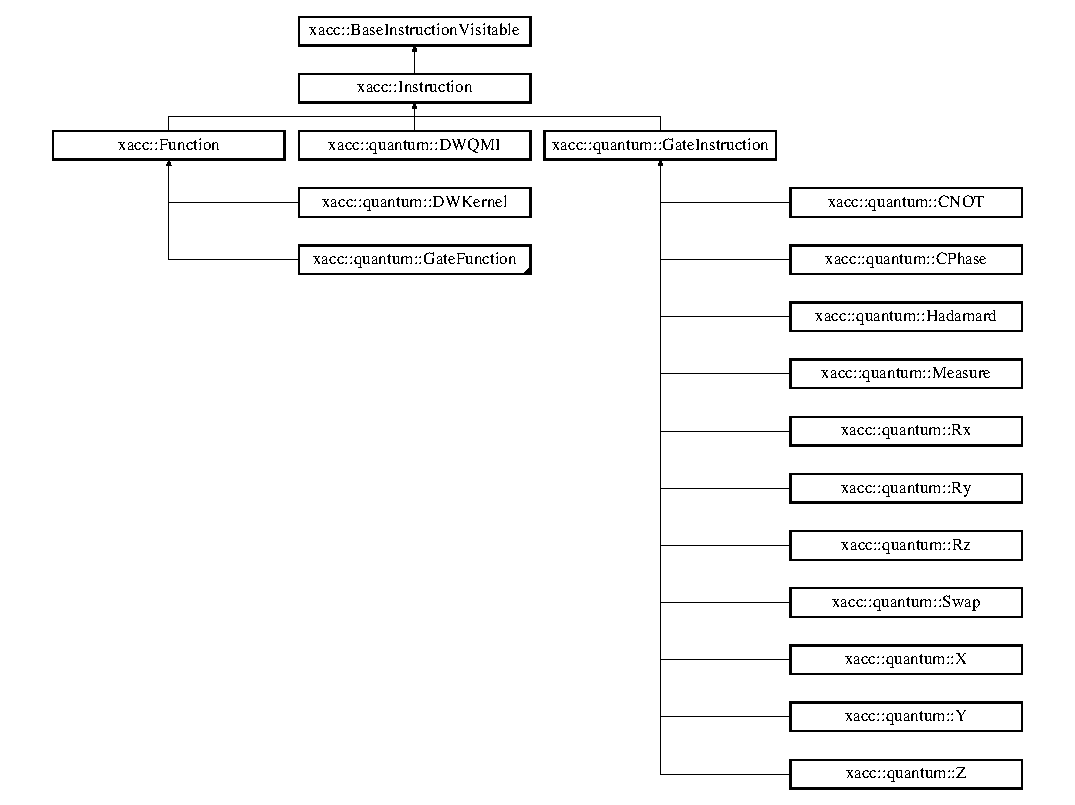
\includegraphics[height=10.370370cm]{a01155}
\end{center}
\end{figure}
\subsection*{Public Member Functions}
\begin{DoxyCompactItemize}
\item 
virtual const std\+::string \hyperlink{a01155_ac7ff23f693e2276edbf3fdac5452792c}{get\+Name} ()=0
\item 
virtual const std\+::string \hyperlink{a01155_ae94c2d089908294c1d410b14c96817ae}{to\+String} (const std\+::string \&buffer\+Var\+Name)=0
\item 
virtual const std\+::vector$<$ int $>$ \hyperlink{a01155_a819f32e94c3e1c9e69a0061aaf8d86dc}{bits} ()=0
\item 
virtual Instruction\+Parameter \hyperlink{a01155_aa0d9de97a4833a042379647f83c33ab6}{get\+Parameter} (const int idx)=0
\item 
virtual std\+::vector$<$ Instruction\+Parameter $>$ \hyperlink{a01155_aeb67c67713896e8f27a5c7dd531f3340}{get\+Parameters} ()=0
\item 
virtual void \hyperlink{a01155_a407a0ac662fa0b1ec3e301e8ff9bade7}{set\+Parameter} (const int idx, Instruction\+Parameter \&isnt)=0
\item 
virtual const int \hyperlink{a01155_ad54585d13c04ffd20296fff7ab8107ff}{n\+Parameters} ()=0
\item 
virtual bool \hyperlink{a01155_a7b24d8ae485369fc2b2df7a3224a5e26}{is\+Parameterized} ()
\item 
virtual bool \hyperlink{a01155_a4383f1036d0fcfe890ab9c613dbd5f38}{is\+Composite} ()
\item 
virtual bool \hyperlink{a01155_ad02a1cf7220577124720b7a51424cea7}{is\+Enabled} ()
\item 
virtual void \hyperlink{a01155_a6e528da15e05a94cc1d7db268c483271}{disable} ()
\item 
virtual void \hyperlink{a01155_a0b4f2e5a591af28342a3c08e4305e24f}{enable} ()
\item 
virtual \hyperlink{a01155_ae22c935e8113bce63d1d0e214cda4d61}{$\sim$\+Instruction} ()
\end{DoxyCompactItemize}
\subsection*{Additional Inherited Members}


\subsection{Detailed Description}
The \hyperlink{a01155}{Instruction} interface is the base of all X\+A\+CC Intermediate Representation Instructions for post-\/\+Moore\textquotesingle{}s law accelerated computing. The \hyperlink{a01155}{Instruction}, at its core, provides an \hyperlink{a01155}{Instruction} name and a set of next-\/gen bits that the \hyperlink{a01155}{Instruction} operates on. Instructions can also be enabled or disabled. Instructions implement \hyperlink{a01171}{Base\+Instruction\+Visitable} to enable visitor pattern functionality across all \hyperlink{a01155}{Instruction} subclasses.

\hyperlink{a01155}{Instruction} can also expose 0 to N Instruction\+Parameters. Instruction\+Parameters can be an int, double, float, or string. 

\subsection{Constructor \& Destructor Documentation}
\mbox{\Hypertarget{a01155_ae22c935e8113bce63d1d0e214cda4d61}\label{a01155_ae22c935e8113bce63d1d0e214cda4d61}} 
\index{xacc\+::\+Instruction@{xacc\+::\+Instruction}!````~Instruction@{$\sim$\+Instruction}}
\index{````~Instruction@{$\sim$\+Instruction}!xacc\+::\+Instruction@{xacc\+::\+Instruction}}
\subsubsection{\texorpdfstring{$\sim$\+Instruction()}{~Instruction()}}
{\footnotesize\ttfamily virtual xacc\+::\+Instruction\+::$\sim$\+Instruction (\begin{DoxyParamCaption}{ }\end{DoxyParamCaption})\hspace{0.3cm}{\ttfamily [inline]}, {\ttfamily [virtual]}}

The destructor 

\subsection{Member Function Documentation}
\mbox{\Hypertarget{a01155_a819f32e94c3e1c9e69a0061aaf8d86dc}\label{a01155_a819f32e94c3e1c9e69a0061aaf8d86dc}} 
\index{xacc\+::\+Instruction@{xacc\+::\+Instruction}!bits@{bits}}
\index{bits@{bits}!xacc\+::\+Instruction@{xacc\+::\+Instruction}}
\subsubsection{\texorpdfstring{bits()}{bits()}}
{\footnotesize\ttfamily virtual const std\+::vector$<$int$>$ xacc\+::\+Instruction\+::bits (\begin{DoxyParamCaption}{ }\end{DoxyParamCaption})\hspace{0.3cm}{\ttfamily [pure virtual]}}

Return the indices of the bits that this \hyperlink{a01155}{Instruction} operates on.

\begin{DoxyReturn}{Returns}
bits The bits this \hyperlink{a01155}{Instruction} operates on. 
\end{DoxyReturn}


Implemented in \hyperlink{a01011_aba03de68b76a9e120705c3c389c714a1}{xacc\+::quantum\+::\+Gate\+Function}, \hyperlink{a00983_adae68964db6acd8b4c2267c270a8ec58}{xacc\+::quantum\+::\+D\+W\+Kernel}, \hyperlink{a01015_ad32ad03dfc516e00093030e60178003d}{xacc\+::quantum\+::\+Gate\+Instruction}, and \hyperlink{a00987_a76939c29e4763d10c57ea9a270229421}{xacc\+::quantum\+::\+D\+W\+Q\+MI}.

\mbox{\Hypertarget{a01155_a6e528da15e05a94cc1d7db268c483271}\label{a01155_a6e528da15e05a94cc1d7db268c483271}} 
\index{xacc\+::\+Instruction@{xacc\+::\+Instruction}!disable@{disable}}
\index{disable@{disable}!xacc\+::\+Instruction@{xacc\+::\+Instruction}}
\subsubsection{\texorpdfstring{disable()}{disable()}}
{\footnotesize\ttfamily virtual void xacc\+::\+Instruction\+::disable (\begin{DoxyParamCaption}{ }\end{DoxyParamCaption})\hspace{0.3cm}{\ttfamily [inline]}, {\ttfamily [virtual]}}

Disable this \hyperlink{a01155}{Instruction} 

Reimplemented in \hyperlink{a00987_af6d9120d8f60984767a330d5cfe9140f}{xacc\+::quantum\+::\+D\+W\+Q\+MI}, and \hyperlink{a01015_a63ce138dd71fb43d303f5600fefb7215}{xacc\+::quantum\+::\+Gate\+Instruction}.

\mbox{\Hypertarget{a01155_a0b4f2e5a591af28342a3c08e4305e24f}\label{a01155_a0b4f2e5a591af28342a3c08e4305e24f}} 
\index{xacc\+::\+Instruction@{xacc\+::\+Instruction}!enable@{enable}}
\index{enable@{enable}!xacc\+::\+Instruction@{xacc\+::\+Instruction}}
\subsubsection{\texorpdfstring{enable()}{enable()}}
{\footnotesize\ttfamily virtual void xacc\+::\+Instruction\+::enable (\begin{DoxyParamCaption}{ }\end{DoxyParamCaption})\hspace{0.3cm}{\ttfamily [inline]}, {\ttfamily [virtual]}}

Enable this \hyperlink{a01155}{Instruction}. 

Reimplemented in \hyperlink{a00987_ae4f563cead75aaa43f06db83e90ee855}{xacc\+::quantum\+::\+D\+W\+Q\+MI}, and \hyperlink{a01015_a7a80474b7fd465271b3313432db2e608}{xacc\+::quantum\+::\+Gate\+Instruction}.

\mbox{\Hypertarget{a01155_ac7ff23f693e2276edbf3fdac5452792c}\label{a01155_ac7ff23f693e2276edbf3fdac5452792c}} 
\index{xacc\+::\+Instruction@{xacc\+::\+Instruction}!get\+Name@{get\+Name}}
\index{get\+Name@{get\+Name}!xacc\+::\+Instruction@{xacc\+::\+Instruction}}
\subsubsection{\texorpdfstring{get\+Name()}{getName()}}
{\footnotesize\ttfamily virtual const std\+::string xacc\+::\+Instruction\+::get\+Name (\begin{DoxyParamCaption}{ }\end{DoxyParamCaption})\hspace{0.3cm}{\ttfamily [pure virtual]}}

Return the name of this \hyperlink{a01155}{Instruction}

\begin{DoxyReturn}{Returns}
name The name of this \hyperlink{a01155}{Instruction} 
\end{DoxyReturn}


Implemented in \hyperlink{a01011_af42efb6191267164717d53c469e15d3a}{xacc\+::quantum\+::\+Gate\+Function}, \hyperlink{a00983_a7f0c4d3c73029566561cf56a474bcbbd}{xacc\+::quantum\+::\+D\+W\+Kernel}, \hyperlink{a01015_a0db03b9e46eeba1134f0ca2b83ccc842}{xacc\+::quantum\+::\+Gate\+Instruction}, and \hyperlink{a00987_ad93428eb61adade7bb99c7633bb02aca}{xacc\+::quantum\+::\+D\+W\+Q\+MI}.

\mbox{\Hypertarget{a01155_aa0d9de97a4833a042379647f83c33ab6}\label{a01155_aa0d9de97a4833a042379647f83c33ab6}} 
\index{xacc\+::\+Instruction@{xacc\+::\+Instruction}!get\+Parameter@{get\+Parameter}}
\index{get\+Parameter@{get\+Parameter}!xacc\+::\+Instruction@{xacc\+::\+Instruction}}
\subsubsection{\texorpdfstring{get\+Parameter()}{getParameter()}}
{\footnotesize\ttfamily virtual Instruction\+Parameter xacc\+::\+Instruction\+::get\+Parameter (\begin{DoxyParamCaption}\item[{const int}]{idx }\end{DoxyParamCaption})\hspace{0.3cm}{\ttfamily [pure virtual]}}

Return this \hyperlink{a01155}{Instruction}\textquotesingle{}s parameter at the given index.


\begin{DoxyParams}{Parameters}
{\em idx} & The index of the parameter. \\
\hline
\end{DoxyParams}
\begin{DoxyReturn}{Returns}
param The Instruction\+Parameter at the given index. 
\end{DoxyReturn}


Implemented in \hyperlink{a01011_a5991903323e412777bedc4f0c862eb63}{xacc\+::quantum\+::\+Gate\+Function}, \hyperlink{a01015_addd6185279fe99fbdc3d4efd96e42162}{xacc\+::quantum\+::\+Gate\+Instruction}, \hyperlink{a00983_a81711b7db284aba35d6952e4d1d15d41}{xacc\+::quantum\+::\+D\+W\+Kernel}, and \hyperlink{a00987_aa15882df55d3f0af3a2ec9d72a2db4c0}{xacc\+::quantum\+::\+D\+W\+Q\+MI}.

\mbox{\Hypertarget{a01155_aeb67c67713896e8f27a5c7dd531f3340}\label{a01155_aeb67c67713896e8f27a5c7dd531f3340}} 
\index{xacc\+::\+Instruction@{xacc\+::\+Instruction}!get\+Parameters@{get\+Parameters}}
\index{get\+Parameters@{get\+Parameters}!xacc\+::\+Instruction@{xacc\+::\+Instruction}}
\subsubsection{\texorpdfstring{get\+Parameters()}{getParameters()}}
{\footnotesize\ttfamily virtual std\+::vector$<$Instruction\+Parameter$>$ xacc\+::\+Instruction\+::get\+Parameters (\begin{DoxyParamCaption}{ }\end{DoxyParamCaption})\hspace{0.3cm}{\ttfamily [pure virtual]}}

Return all of this \hyperlink{a01155}{Instruction}\textquotesingle{}s parameters.

\begin{DoxyReturn}{Returns}
params This instructions parameters. 
\end{DoxyReturn}


Implemented in \hyperlink{a01011_af7aabfe699a4dced576ff7fafff969d5}{xacc\+::quantum\+::\+Gate\+Function}, \hyperlink{a01015_a8584444f9577283f6844ab32bdc4db72}{xacc\+::quantum\+::\+Gate\+Instruction}, \hyperlink{a00983_a829462cff34e2257da06afd8a2051a8e}{xacc\+::quantum\+::\+D\+W\+Kernel}, and \hyperlink{a00987_a896d9a4e2876129c2cf81ef028daf1ff}{xacc\+::quantum\+::\+D\+W\+Q\+MI}.

\mbox{\Hypertarget{a01155_a4383f1036d0fcfe890ab9c613dbd5f38}\label{a01155_a4383f1036d0fcfe890ab9c613dbd5f38}} 
\index{xacc\+::\+Instruction@{xacc\+::\+Instruction}!is\+Composite@{is\+Composite}}
\index{is\+Composite@{is\+Composite}!xacc\+::\+Instruction@{xacc\+::\+Instruction}}
\subsubsection{\texorpdfstring{is\+Composite()}{isComposite()}}
{\footnotesize\ttfamily virtual bool xacc\+::\+Instruction\+::is\+Composite (\begin{DoxyParamCaption}{ }\end{DoxyParamCaption})\hspace{0.3cm}{\ttfamily [inline]}, {\ttfamily [virtual]}}

Returns true if this \hyperlink{a01155}{Instruction} is composite, ie, contains other Instructions.

\begin{DoxyReturn}{Returns}
is\+Composite True if this is a composite \hyperlink{a01155}{Instruction} 
\end{DoxyReturn}


Reimplemented in \hyperlink{a00987_ad2b3b4ee72dee48150bf78d92c52e5e0}{xacc\+::quantum\+::\+D\+W\+Q\+MI}, and \hyperlink{a01151_aa75500c657b5c3e0e36213e1506aad97}{xacc\+::\+Function}.

\mbox{\Hypertarget{a01155_ad02a1cf7220577124720b7a51424cea7}\label{a01155_ad02a1cf7220577124720b7a51424cea7}} 
\index{xacc\+::\+Instruction@{xacc\+::\+Instruction}!is\+Enabled@{is\+Enabled}}
\index{is\+Enabled@{is\+Enabled}!xacc\+::\+Instruction@{xacc\+::\+Instruction}}
\subsubsection{\texorpdfstring{is\+Enabled()}{isEnabled()}}
{\footnotesize\ttfamily virtual bool xacc\+::\+Instruction\+::is\+Enabled (\begin{DoxyParamCaption}{ }\end{DoxyParamCaption})\hspace{0.3cm}{\ttfamily [inline]}, {\ttfamily [virtual]}}

Returns true if this \hyperlink{a01155}{Instruction} is enabled

\begin{DoxyReturn}{Returns}
enabled True if this \hyperlink{a01155}{Instruction} is enabled. 
\end{DoxyReturn}


Reimplemented in \hyperlink{a00987_aea76901b30d85172ef26fc317b4c0ed7}{xacc\+::quantum\+::\+D\+W\+Q\+MI}, and \hyperlink{a01015_a0a821be322b0c848b01c55f91fc8f484}{xacc\+::quantum\+::\+Gate\+Instruction}.

\mbox{\Hypertarget{a01155_a7b24d8ae485369fc2b2df7a3224a5e26}\label{a01155_a7b24d8ae485369fc2b2df7a3224a5e26}} 
\index{xacc\+::\+Instruction@{xacc\+::\+Instruction}!is\+Parameterized@{is\+Parameterized}}
\index{is\+Parameterized@{is\+Parameterized}!xacc\+::\+Instruction@{xacc\+::\+Instruction}}
\subsubsection{\texorpdfstring{is\+Parameterized()}{isParameterized()}}
{\footnotesize\ttfamily virtual bool xacc\+::\+Instruction\+::is\+Parameterized (\begin{DoxyParamCaption}{ }\end{DoxyParamCaption})\hspace{0.3cm}{\ttfamily [inline]}, {\ttfamily [virtual]}}

Return true if this \hyperlink{a01155}{Instruction} is parameterized.

\begin{DoxyReturn}{Returns}
parameterized True if this \hyperlink{a01155}{Instruction} has parameters. 
\end{DoxyReturn}


Reimplemented in \hyperlink{a01011_afad47903e0ed55ddbfa827ef8408a94b}{xacc\+::quantum\+::\+Gate\+Function}, \hyperlink{a01015_afe7aeeb398262931e156bcb3950f8188}{xacc\+::quantum\+::\+Gate\+Instruction}, \hyperlink{a00983_a8957ea368244ed4a4ebd85f6bfecb785}{xacc\+::quantum\+::\+D\+W\+Kernel}, and \hyperlink{a00987_aee43b2e499f122dfe250b529a3f77add}{xacc\+::quantum\+::\+D\+W\+Q\+MI}.

\mbox{\Hypertarget{a01155_ad54585d13c04ffd20296fff7ab8107ff}\label{a01155_ad54585d13c04ffd20296fff7ab8107ff}} 
\index{xacc\+::\+Instruction@{xacc\+::\+Instruction}!n\+Parameters@{n\+Parameters}}
\index{n\+Parameters@{n\+Parameters}!xacc\+::\+Instruction@{xacc\+::\+Instruction}}
\subsubsection{\texorpdfstring{n\+Parameters()}{nParameters()}}
{\footnotesize\ttfamily virtual const int xacc\+::\+Instruction\+::n\+Parameters (\begin{DoxyParamCaption}{ }\end{DoxyParamCaption})\hspace{0.3cm}{\ttfamily [pure virtual]}}

Return the number of Instruction\+Parameters this \hyperlink{a01155}{Instruction} contains.

\begin{DoxyReturn}{Returns}
n\+Insts The number of instructions. 
\end{DoxyReturn}


Implemented in \hyperlink{a01011_ad0bffcbc0884d81d6bdddf55385fc6c9}{xacc\+::quantum\+::\+Gate\+Function}, \hyperlink{a01015_a3752912b2c402668ca4814e21d4bbd26}{xacc\+::quantum\+::\+Gate\+Instruction}, \hyperlink{a00983_a029429948329b94c1d89f32cf5c486d4}{xacc\+::quantum\+::\+D\+W\+Kernel}, and \hyperlink{a00987_afdfc8b852ba29c2b21c5c368098ffc4c}{xacc\+::quantum\+::\+D\+W\+Q\+MI}.

\mbox{\Hypertarget{a01155_a407a0ac662fa0b1ec3e301e8ff9bade7}\label{a01155_a407a0ac662fa0b1ec3e301e8ff9bade7}} 
\index{xacc\+::\+Instruction@{xacc\+::\+Instruction}!set\+Parameter@{set\+Parameter}}
\index{set\+Parameter@{set\+Parameter}!xacc\+::\+Instruction@{xacc\+::\+Instruction}}
\subsubsection{\texorpdfstring{set\+Parameter()}{setParameter()}}
{\footnotesize\ttfamily virtual void xacc\+::\+Instruction\+::set\+Parameter (\begin{DoxyParamCaption}\item[{const int}]{idx,  }\item[{Instruction\+Parameter \&}]{isnt }\end{DoxyParamCaption})\hspace{0.3cm}{\ttfamily [pure virtual]}}

Set this \hyperlink{a01155}{Instruction}\textquotesingle{}s parameter at the given index.


\begin{DoxyParams}{Parameters}
{\em idx} & The index of the parameter \\
\hline
{\em inst} & The instruction. \\
\hline
\end{DoxyParams}


Implemented in \hyperlink{a01011_ab8d9789b46e92e27a9d7c9c5b7e3683c}{xacc\+::quantum\+::\+Gate\+Function}, \hyperlink{a01015_afb8f7582d7520c77d61b9016753f5669}{xacc\+::quantum\+::\+Gate\+Instruction}, \hyperlink{a00983_adf89cdd1f54e183c4cff36b338b2be8d}{xacc\+::quantum\+::\+D\+W\+Kernel}, and \hyperlink{a00987_a194b5b9f58262774fde0285f4c3f60af}{xacc\+::quantum\+::\+D\+W\+Q\+MI}.

\mbox{\Hypertarget{a01155_ae94c2d089908294c1d410b14c96817ae}\label{a01155_ae94c2d089908294c1d410b14c96817ae}} 
\index{xacc\+::\+Instruction@{xacc\+::\+Instruction}!to\+String@{to\+String}}
\index{to\+String@{to\+String}!xacc\+::\+Instruction@{xacc\+::\+Instruction}}
\subsubsection{\texorpdfstring{to\+String()}{toString()}}
{\footnotesize\ttfamily virtual const std\+::string xacc\+::\+Instruction\+::to\+String (\begin{DoxyParamCaption}\item[{const std\+::string \&}]{buffer\+Var\+Name }\end{DoxyParamCaption})\hspace{0.3cm}{\ttfamily [pure virtual]}}

Persist this \hyperlink{a01155}{Instruction} to an assembly-\/like string.


\begin{DoxyParams}{Parameters}
{\em buffer\+Var\+Name} & The name of the \hyperlink{a01123}{Accelerator\+Buffer} \\
\hline
\end{DoxyParams}
\begin{DoxyReturn}{Returns}
str The assembly-\/like string. 
\end{DoxyReturn}


Implemented in \hyperlink{a01011_aa1950776ae84bad2d0795a0441f910e7}{xacc\+::quantum\+::\+Gate\+Function}, \hyperlink{a00983_adbc3fdd080ebba20bc620b8832979f16}{xacc\+::quantum\+::\+D\+W\+Kernel}, \hyperlink{a01015_a089a5da67ff40ac1a6f56e64589822d9}{xacc\+::quantum\+::\+Gate\+Instruction}, \hyperlink{a00987_a8d8742bb6743cf6e49f95966d05bbec2}{xacc\+::quantum\+::\+D\+W\+Q\+MI}, \hyperlink{a01047_a1c51a5d68294dcb2ba1a9fbea63a730f}{xacc\+::quantum\+::\+Measure}, and \hyperlink{a01035_aca7a5f849fece6fc28a904efee9a3370}{xacc\+::quantum\+::\+Conditional\+Function}.



The documentation for this class was generated from the following file\+:\begin{DoxyCompactItemize}
\item 
Instruction.\+hpp\end{DoxyCompactItemize}

\hypertarget{a01159}{}\section{xacc\+:\+:Program Class Reference}
\label{a01159}\index{xacc\+::\+Program@{xacc\+::\+Program}}


{\ttfamily \#include $<$Program.\+hpp$>$}

\subsection*{Public Member Functions}
\begin{DoxyCompactItemize}
\item 
\hyperlink{a01159_a6d20079fde67a3ef145315e762249115}{Program} (std\+::shared\+\_\+ptr$<$ \hyperlink{a01087}{Accelerator} $>$ acc, const std\+::string \&source\+File)
\item 
{\footnotesize template$<$typename ... Runtime\+Args$>$ }\\std\+::function$<$ void(std\+::shared\+\_\+ptr$<$ \hyperlink{a01099}{Accelerator\+Buffer} $>$, Runtime\+Args...)$>$ \hyperlink{a01159_abf5023c9f01cac8a506bdef86760e8f1}{get\+Kernel} (const std\+::string \&kernel\+Name)
\end{DoxyCompactItemize}
\subsection*{Protected Member Functions}
\begin{DoxyCompactItemize}
\item 
void \hyperlink{a01159_a53079c7886c0be065968bcf6674d1516}{build} ()
\end{DoxyCompactItemize}
\subsection*{Protected Attributes}
\begin{DoxyCompactItemize}
\item 
std\+::string \hyperlink{a01159_aae78160f9f9e52a3e0c9b342996a7202}{src}
\item 
std\+::shared\+\_\+ptr$<$ \hyperlink{a01087}{Accelerator} $>$ \hyperlink{a01159_a10c948629c84f23dd426c04a9a518155}{accelerator}
\item 
std\+::shared\+\_\+ptr$<$ \hyperlink{a01151}{IR} $>$ \hyperlink{a01159_a5681f0989fc1c3fced8e30e815d6511c}{xacc\+IR}
\item 
std\+::shared\+\_\+ptr$<$ \hyperlink{a01103}{Compiler} $>$ \hyperlink{a01159_a0d2ae2522bb0daad0eea7871fc4e2061}{compiler}
\end{DoxyCompactItemize}


\subsection{Detailed Description}
The \hyperlink{a01159}{Program} is the main entrypoint for the X\+A\+CC A\+PI. Users with accelerator kernels must construct a valid \hyperlink{a01159}{Program} to be compiled and executed on the attached accelerator. Programs must be given the \hyperlink{a01087}{Accelerator} reference to be used and kernel source code at construction time. 

\subsection{Constructor \& Destructor Documentation}
\mbox{\Hypertarget{a01159_a6d20079fde67a3ef145315e762249115}\label{a01159_a6d20079fde67a3ef145315e762249115}} 
\index{xacc\+::\+Program@{xacc\+::\+Program}!Program@{Program}}
\index{Program@{Program}!xacc\+::\+Program@{xacc\+::\+Program}}
\subsubsection{\texorpdfstring{Program()}{Program()}}
{\footnotesize\ttfamily xacc\+::\+Program\+::\+Program (\begin{DoxyParamCaption}\item[{std\+::shared\+\_\+ptr$<$ \hyperlink{a01087}{Accelerator} $>$}]{acc,  }\item[{const std\+::string \&}]{source\+File }\end{DoxyParamCaption})\hspace{0.3cm}{\ttfamily [inline]}}

The Constructor, takes the \hyperlink{a01087}{Accelerator} to execute on, and the source to compile and execute


\begin{DoxyParams}{Parameters}
{\em acc} & Attached \hyperlink{a01087}{Accelerator} to execute \\
\hline
{\em source\+File} & The kernel source code \\
\hline
\end{DoxyParams}


\subsection{Member Function Documentation}
\mbox{\Hypertarget{a01159_a53079c7886c0be065968bcf6674d1516}\label{a01159_a53079c7886c0be065968bcf6674d1516}} 
\index{xacc\+::\+Program@{xacc\+::\+Program}!build@{build}}
\index{build@{build}!xacc\+::\+Program@{xacc\+::\+Program}}
\subsubsection{\texorpdfstring{build()}{build()}}
{\footnotesize\ttfamily void xacc\+::\+Program\+::build (\begin{DoxyParamCaption}{ }\end{DoxyParamCaption})\hspace{0.3cm}{\ttfamily [inline]}, {\ttfamily [protected]}}

Execute the compilation mechanism on the provided program source kernel code to produce X\+A\+CC \hyperlink{a01151}{IR} that can be executed on the attached \hyperlink{a01087}{Accelerator}. \mbox{\Hypertarget{a01159_abf5023c9f01cac8a506bdef86760e8f1}\label{a01159_abf5023c9f01cac8a506bdef86760e8f1}} 
\index{xacc\+::\+Program@{xacc\+::\+Program}!get\+Kernel@{get\+Kernel}}
\index{get\+Kernel@{get\+Kernel}!xacc\+::\+Program@{xacc\+::\+Program}}
\subsubsection{\texorpdfstring{get\+Kernel()}{getKernel()}}
{\footnotesize\ttfamily template$<$typename ... Runtime\+Args$>$ \\
std\+::function$<$void(std\+::shared\+\_\+ptr$<$\hyperlink{a01099}{Accelerator\+Buffer}$>$, Runtime\+Args...)$>$ xacc\+::\+Program\+::get\+Kernel (\begin{DoxyParamCaption}\item[{const std\+::string \&}]{kernel\+Name }\end{DoxyParamCaption})\hspace{0.3cm}{\ttfamily [inline]}}

Return an executable version of the quantum kernel referenced by the kernel\+Name string.


\begin{DoxyParams}{Parameters}
{\em name} & \\
\hline
{\em args} & \\
\hline
\end{DoxyParams}
\begin{DoxyReturn}{Returns}

\end{DoxyReturn}


\subsection{Member Data Documentation}
\mbox{\Hypertarget{a01159_a10c948629c84f23dd426c04a9a518155}\label{a01159_a10c948629c84f23dd426c04a9a518155}} 
\index{xacc\+::\+Program@{xacc\+::\+Program}!accelerator@{accelerator}}
\index{accelerator@{accelerator}!xacc\+::\+Program@{xacc\+::\+Program}}
\subsubsection{\texorpdfstring{accelerator}{accelerator}}
{\footnotesize\ttfamily std\+::shared\+\_\+ptr$<$\hyperlink{a01087}{Accelerator}$>$ xacc\+::\+Program\+::accelerator\hspace{0.3cm}{\ttfamily [protected]}}

Reference to the attached \hyperlink{a01087}{Accelerator} to use in this compilation and execution \mbox{\Hypertarget{a01159_a0d2ae2522bb0daad0eea7871fc4e2061}\label{a01159_a0d2ae2522bb0daad0eea7871fc4e2061}} 
\index{xacc\+::\+Program@{xacc\+::\+Program}!compiler@{compiler}}
\index{compiler@{compiler}!xacc\+::\+Program@{xacc\+::\+Program}}
\subsubsection{\texorpdfstring{compiler}{compiler}}
{\footnotesize\ttfamily std\+::shared\+\_\+ptr$<$\hyperlink{a01103}{Compiler}$>$ xacc\+::\+Program\+::compiler\hspace{0.3cm}{\ttfamily [protected]}}

Reference to the compiler \mbox{\Hypertarget{a01159_aae78160f9f9e52a3e0c9b342996a7202}\label{a01159_aae78160f9f9e52a3e0c9b342996a7202}} 
\index{xacc\+::\+Program@{xacc\+::\+Program}!src@{src}}
\index{src@{src}!xacc\+::\+Program@{xacc\+::\+Program}}
\subsubsection{\texorpdfstring{src}{src}}
{\footnotesize\ttfamily std\+::string xacc\+::\+Program\+::src\hspace{0.3cm}{\ttfamily [protected]}}

Reference to the source accelerator kernel code to be compiled and executed \mbox{\Hypertarget{a01159_a5681f0989fc1c3fced8e30e815d6511c}\label{a01159_a5681f0989fc1c3fced8e30e815d6511c}} 
\index{xacc\+::\+Program@{xacc\+::\+Program}!xacc\+IR@{xacc\+IR}}
\index{xacc\+IR@{xacc\+IR}!xacc\+::\+Program@{xacc\+::\+Program}}
\subsubsection{\texorpdfstring{xacc\+IR}{xaccIR}}
{\footnotesize\ttfamily std\+::shared\+\_\+ptr$<$\hyperlink{a01151}{IR}$>$ xacc\+::\+Program\+::xacc\+IR\hspace{0.3cm}{\ttfamily [protected]}}

Reference to the X\+A\+CC \hyperlink{a01151}{IR} instance that is created by the \hyperlink{a01103}{Compiler} 

The documentation for this class was generated from the following file\+:\begin{DoxyCompactItemize}
\item 
Program.\+hpp\end{DoxyCompactItemize}

\hypertarget{a01171}{}\section{xacc\+:\+:quantum\+:\+:Gate\+Q\+IR Class Reference}
\label{a01171}\index{xacc\+::quantum\+::\+Gate\+Q\+IR@{xacc\+::quantum\+::\+Gate\+Q\+IR}}


{\ttfamily \#include $<$Gate\+Q\+I\+R.\+hpp$>$}

Inheritance diagram for xacc\+:\+:quantum\+:\+:Gate\+Q\+IR\+:\begin{figure}[H]
\begin{center}
\leavevmode
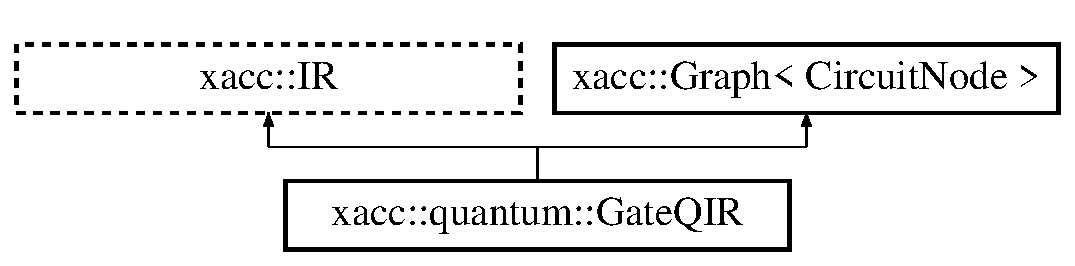
\includegraphics[height=2.000000cm]{a01171}
\end{center}
\end{figure}
\subsection*{Public Member Functions}
\begin{DoxyCompactItemize}
\item 
\hyperlink{a01171_afb99f610a6b123538c659169c131a634}{Gate\+Q\+IR} ()
\item 
virtual void \hyperlink{a01171_ad1ddd6105346dd9fc78648fd812285ed}{generate\+Graph} (const std\+::string \&kernel\+Name)
\item 
virtual void \hyperlink{a01171_aa6ed2cf2cbcfec8105c327a4fa95346f}{add\+Kernel} (std\+::shared\+\_\+ptr$<$ \hyperlink{a01475}{Function} $>$ kernel)
\item 
\mbox{\Hypertarget{a01171_aca6be85526b14f500e7f98954dd6da5c}\label{a01171_aca6be85526b14f500e7f98954dd6da5c}} 
virtual const int {\bfseries number\+Of\+Kernels} ()
\item 
virtual std\+::shared\+\_\+ptr$<$ \hyperlink{a01475}{Function} $>$ \hyperlink{a01171_a194758b6edcc3ae0c7fe8004f9bfe690}{get\+Kernel} (const std\+::string \&name)
\item 
virtual bool \hyperlink{a01171_a692f95099caa7c024110a3f035941dca}{kernel\+Exists} (const std\+::string \&name)
\item 
virtual std\+::string \hyperlink{a01171_a7153f7e9f516d43af3d5d4f95d60bd86}{to\+Assembly\+String} (const std\+::string \&kernel\+Name, const std\+::string \&acc\+Buffer\+Var\+Name)
\item 
virtual void \hyperlink{a01171_a40e1d07e4dfd3794ef53fca3cdbdca61}{persist} (std\+::ostream \&out\+Stream)
\item 
virtual void \hyperlink{a01171_a07f26eeb362ac480d20da6cdc8c8fb39}{load} (std\+::istream \&in\+Stream)
\item 
virtual void \hyperlink{a01171_a26019e2f1e13e64645e29aee86ac58b1}{read} (std\+::istream \&stream)
\item 
virtual std\+::vector$<$ std\+::shared\+\_\+ptr$<$ \hyperlink{a01475}{Function} $>$ $>$ \hyperlink{a01171_a4ace7ee5ebef84b1f39aaf5ed12c6cc6}{get\+Kernels} ()
\item 
virtual \hyperlink{a01171_ac88db03f1dd29e2d36aaa6c01a130008}{$\sim$\+Gate\+Q\+IR} ()
\end{DoxyCompactItemize}
\subsection*{Protected Attributes}
\begin{DoxyCompactItemize}
\item 
std\+::vector$<$ std\+::shared\+\_\+ptr$<$ \hyperlink{a01475}{Function} $>$ $>$ \hyperlink{a01171_ae75a4af0ce455eee1ce316c16426a661}{kernels}
\end{DoxyCompactItemize}


\subsection{Detailed Description}
The \hyperlink{a01171}{Gate\+Q\+IR} is an implementation of the Q\+IR for gate model quantum computing. It provides a \hyperlink{a01535}{Graph} node type that models a quantum circuit gate (\hyperlink{a01167}{Circuit\+Node}). 

\subsection{Constructor \& Destructor Documentation}
\mbox{\Hypertarget{a01171_afb99f610a6b123538c659169c131a634}\label{a01171_afb99f610a6b123538c659169c131a634}} 
\index{xacc\+::quantum\+::\+Gate\+Q\+IR@{xacc\+::quantum\+::\+Gate\+Q\+IR}!Gate\+Q\+IR@{Gate\+Q\+IR}}
\index{Gate\+Q\+IR@{Gate\+Q\+IR}!xacc\+::quantum\+::\+Gate\+Q\+IR@{xacc\+::quantum\+::\+Gate\+Q\+IR}}
\subsubsection{\texorpdfstring{Gate\+Q\+I\+R()}{GateQIR()}}
{\footnotesize\ttfamily xacc\+::quantum\+::\+Gate\+Q\+I\+R\+::\+Gate\+Q\+IR (\begin{DoxyParamCaption}{ }\end{DoxyParamCaption})\hspace{0.3cm}{\ttfamily [inline]}}

The nullary Constructor \mbox{\Hypertarget{a01171_ac88db03f1dd29e2d36aaa6c01a130008}\label{a01171_ac88db03f1dd29e2d36aaa6c01a130008}} 
\index{xacc\+::quantum\+::\+Gate\+Q\+IR@{xacc\+::quantum\+::\+Gate\+Q\+IR}!````~Gate\+Q\+IR@{$\sim$\+Gate\+Q\+IR}}
\index{````~Gate\+Q\+IR@{$\sim$\+Gate\+Q\+IR}!xacc\+::quantum\+::\+Gate\+Q\+IR@{xacc\+::quantum\+::\+Gate\+Q\+IR}}
\subsubsection{\texorpdfstring{$\sim$\+Gate\+Q\+I\+R()}{~GateQIR()}}
{\footnotesize\ttfamily virtual xacc\+::quantum\+::\+Gate\+Q\+I\+R\+::$\sim$\+Gate\+Q\+IR (\begin{DoxyParamCaption}{ }\end{DoxyParamCaption})\hspace{0.3cm}{\ttfamily [inline]}, {\ttfamily [virtual]}}

The destructor 

\subsection{Member Function Documentation}
\mbox{\Hypertarget{a01171_aa6ed2cf2cbcfec8105c327a4fa95346f}\label{a01171_aa6ed2cf2cbcfec8105c327a4fa95346f}} 
\index{xacc\+::quantum\+::\+Gate\+Q\+IR@{xacc\+::quantum\+::\+Gate\+Q\+IR}!add\+Kernel@{add\+Kernel}}
\index{add\+Kernel@{add\+Kernel}!xacc\+::quantum\+::\+Gate\+Q\+IR@{xacc\+::quantum\+::\+Gate\+Q\+IR}}
\subsubsection{\texorpdfstring{add\+Kernel()}{addKernel()}}
{\footnotesize\ttfamily virtual void xacc\+::quantum\+::\+Gate\+Q\+I\+R\+::add\+Kernel (\begin{DoxyParamCaption}\item[{std\+::shared\+\_\+ptr$<$ \hyperlink{a01475}{Function} $>$}]{kernel }\end{DoxyParamCaption})\hspace{0.3cm}{\ttfamily [inline]}, {\ttfamily [virtual]}}

Add a quantum function to this intermediate representation. 
\begin{DoxyParams}{Parameters}
{\em kernel} & \\
\hline
\end{DoxyParams}


Implements \hyperlink{a01499_abbbf8e6993c518597de32cd05d49d737}{xacc\+::\+IR}.

\mbox{\Hypertarget{a01171_ad1ddd6105346dd9fc78648fd812285ed}\label{a01171_ad1ddd6105346dd9fc78648fd812285ed}} 
\index{xacc\+::quantum\+::\+Gate\+Q\+IR@{xacc\+::quantum\+::\+Gate\+Q\+IR}!generate\+Graph@{generate\+Graph}}
\index{generate\+Graph@{generate\+Graph}!xacc\+::quantum\+::\+Gate\+Q\+IR@{xacc\+::quantum\+::\+Gate\+Q\+IR}}
\subsubsection{\texorpdfstring{generate\+Graph()}{generateGraph()}}
{\footnotesize\ttfamily void xacc\+::quantum\+::\+Gate\+Q\+I\+R\+::generate\+Graph (\begin{DoxyParamCaption}\item[{const std\+::string \&}]{kernel\+Name }\end{DoxyParamCaption})\hspace{0.3cm}{\ttfamily [virtual]}}

This method takes the list of quantum instructions that this Q\+IR contains and creates a graph representation of the quantum circuit. \mbox{\Hypertarget{a01171_a194758b6edcc3ae0c7fe8004f9bfe690}\label{a01171_a194758b6edcc3ae0c7fe8004f9bfe690}} 
\index{xacc\+::quantum\+::\+Gate\+Q\+IR@{xacc\+::quantum\+::\+Gate\+Q\+IR}!get\+Kernel@{get\+Kernel}}
\index{get\+Kernel@{get\+Kernel}!xacc\+::quantum\+::\+Gate\+Q\+IR@{xacc\+::quantum\+::\+Gate\+Q\+IR}}
\subsubsection{\texorpdfstring{get\+Kernel()}{getKernel()}}
{\footnotesize\ttfamily virtual std\+::shared\+\_\+ptr$<$\hyperlink{a01475}{Function}$>$ xacc\+::quantum\+::\+Gate\+Q\+I\+R\+::get\+Kernel (\begin{DoxyParamCaption}\item[{const std\+::string \&}]{name }\end{DoxyParamCaption})\hspace{0.3cm}{\ttfamily [inline]}, {\ttfamily [virtual]}}

Return the kernel with the given name.


\begin{DoxyParams}{Parameters}
{\em name} & The name of the kernel to return. \\
\hline
\end{DoxyParams}
\begin{DoxyReturn}{Returns}
kernel The kernel with given name. 
\end{DoxyReturn}


Implements \hyperlink{a01499_a6f49b4ba4b3a15142b04873284885f0d}{xacc\+::\+IR}.

\mbox{\Hypertarget{a01171_a4ace7ee5ebef84b1f39aaf5ed12c6cc6}\label{a01171_a4ace7ee5ebef84b1f39aaf5ed12c6cc6}} 
\index{xacc\+::quantum\+::\+Gate\+Q\+IR@{xacc\+::quantum\+::\+Gate\+Q\+IR}!get\+Kernels@{get\+Kernels}}
\index{get\+Kernels@{get\+Kernels}!xacc\+::quantum\+::\+Gate\+Q\+IR@{xacc\+::quantum\+::\+Gate\+Q\+IR}}
\subsubsection{\texorpdfstring{get\+Kernels()}{getKernels()}}
{\footnotesize\ttfamily virtual std\+::vector$<$std\+::shared\+\_\+ptr$<$\hyperlink{a01475}{Function}$>$ $>$ xacc\+::quantum\+::\+Gate\+Q\+I\+R\+::get\+Kernels (\begin{DoxyParamCaption}{ }\end{DoxyParamCaption})\hspace{0.3cm}{\ttfamily [inline]}, {\ttfamily [virtual]}}

Return all of this \hyperlink{a01499}{IR} instance\textquotesingle{}s kernels.

\begin{DoxyReturn}{Returns}
kernels The kernels this \hyperlink{a01499}{IR} contains. 
\end{DoxyReturn}


Implements \hyperlink{a01499_a88c50bfc5b279145360ddc0c3a703b9b}{xacc\+::\+IR}.

\mbox{\Hypertarget{a01171_a692f95099caa7c024110a3f035941dca}\label{a01171_a692f95099caa7c024110a3f035941dca}} 
\index{xacc\+::quantum\+::\+Gate\+Q\+IR@{xacc\+::quantum\+::\+Gate\+Q\+IR}!kernel\+Exists@{kernel\+Exists}}
\index{kernel\+Exists@{kernel\+Exists}!xacc\+::quantum\+::\+Gate\+Q\+IR@{xacc\+::quantum\+::\+Gate\+Q\+IR}}
\subsubsection{\texorpdfstring{kernel\+Exists()}{kernelExists()}}
{\footnotesize\ttfamily virtual bool xacc\+::quantum\+::\+Gate\+Q\+I\+R\+::kernel\+Exists (\begin{DoxyParamCaption}\item[{const std\+::string \&}]{name }\end{DoxyParamCaption})\hspace{0.3cm}{\ttfamily [inline]}, {\ttfamily [virtual]}}

Return true if the kernel with given name exists in this \hyperlink{a01499}{IR}.


\begin{DoxyParams}{Parameters}
{\em name} & The name of the kernel to return. \\
\hline
\end{DoxyParams}
\begin{DoxyReturn}{Returns}
exists True if kernel exists. 
\end{DoxyReturn}


Implements \hyperlink{a01499_afc9ccf5126f3fed19c2e879133b2f6d8}{xacc\+::\+IR}.

\mbox{\Hypertarget{a01171_a07f26eeb362ac480d20da6cdc8c8fb39}\label{a01171_a07f26eeb362ac480d20da6cdc8c8fb39}} 
\index{xacc\+::quantum\+::\+Gate\+Q\+IR@{xacc\+::quantum\+::\+Gate\+Q\+IR}!load@{load}}
\index{load@{load}!xacc\+::quantum\+::\+Gate\+Q\+IR@{xacc\+::quantum\+::\+Gate\+Q\+IR}}
\subsubsection{\texorpdfstring{load()}{load()}}
{\footnotesize\ttfamily void xacc\+::quantum\+::\+Gate\+Q\+I\+R\+::load (\begin{DoxyParamCaption}\item[{std\+::istream \&}]{in\+Stream }\end{DoxyParamCaption})\hspace{0.3cm}{\ttfamily [virtual]}}

Create this \hyperlink{a01499}{IR} instance from the given input stream.


\begin{DoxyParams}{Parameters}
{\em in\+Stream} & \\
\hline
\end{DoxyParams}


Implements \hyperlink{a01499_a444c2e4dc0faac500fb70fa93997e9bc}{xacc\+::\+IR}.

\mbox{\Hypertarget{a01171_a40e1d07e4dfd3794ef53fca3cdbdca61}\label{a01171_a40e1d07e4dfd3794ef53fca3cdbdca61}} 
\index{xacc\+::quantum\+::\+Gate\+Q\+IR@{xacc\+::quantum\+::\+Gate\+Q\+IR}!persist@{persist}}
\index{persist@{persist}!xacc\+::quantum\+::\+Gate\+Q\+IR@{xacc\+::quantum\+::\+Gate\+Q\+IR}}
\subsubsection{\texorpdfstring{persist()}{persist()}}
{\footnotesize\ttfamily void xacc\+::quantum\+::\+Gate\+Q\+I\+R\+::persist (\begin{DoxyParamCaption}\item[{std\+::ostream \&}]{out\+Stream }\end{DoxyParamCaption})\hspace{0.3cm}{\ttfamily [virtual]}}

Persist this \hyperlink{a01499}{IR} instance to the given output stream.


\begin{DoxyParams}{Parameters}
{\em out\+Stream} & \\
\hline
\end{DoxyParams}


Implements \hyperlink{a01499_a414b72224d88473ad6190bb88102a3ea}{xacc\+::\+IR}.

\mbox{\Hypertarget{a01171_a26019e2f1e13e64645e29aee86ac58b1}\label{a01171_a26019e2f1e13e64645e29aee86ac58b1}} 
\index{xacc\+::quantum\+::\+Gate\+Q\+IR@{xacc\+::quantum\+::\+Gate\+Q\+IR}!read@{read}}
\index{read@{read}!xacc\+::quantum\+::\+Gate\+Q\+IR@{xacc\+::quantum\+::\+Gate\+Q\+IR}}
\subsubsection{\texorpdfstring{read()}{read()}}
{\footnotesize\ttfamily void xacc\+::quantum\+::\+Gate\+Q\+I\+R\+::read (\begin{DoxyParamCaption}\item[{std\+::istream \&}]{stream }\end{DoxyParamCaption})\hspace{0.3cm}{\ttfamily [virtual]}}

This is the implementation of the \hyperlink{a01535_abdd3e67dc08c223821d809bc8914164a}{Graph.\+read} method...

Read in a graphviz dot graph from the given input stream. This is left for subclasses.


\begin{DoxyParams}{Parameters}
{\em stream} & \\
\hline
\end{DoxyParams}


Reimplemented from \hyperlink{a01535_abdd3e67dc08c223821d809bc8914164a}{xacc\+::\+Graph$<$ Circuit\+Node $>$}.

\mbox{\Hypertarget{a01171_a7153f7e9f516d43af3d5d4f95d60bd86}\label{a01171_a7153f7e9f516d43af3d5d4f95d60bd86}} 
\index{xacc\+::quantum\+::\+Gate\+Q\+IR@{xacc\+::quantum\+::\+Gate\+Q\+IR}!to\+Assembly\+String@{to\+Assembly\+String}}
\index{to\+Assembly\+String@{to\+Assembly\+String}!xacc\+::quantum\+::\+Gate\+Q\+IR@{xacc\+::quantum\+::\+Gate\+Q\+IR}}
\subsubsection{\texorpdfstring{to\+Assembly\+String()}{toAssemblyString()}}
{\footnotesize\ttfamily std\+::string xacc\+::quantum\+::\+Gate\+Q\+I\+R\+::to\+Assembly\+String (\begin{DoxyParamCaption}\item[{const std\+::string \&}]{kernel\+Name,  }\item[{const std\+::string \&}]{acc\+Buffer\+Var\+Name }\end{DoxyParamCaption})\hspace{0.3cm}{\ttfamily [virtual]}}

Return a string representation of this intermediate representation \begin{DoxyReturn}{Returns}

\end{DoxyReturn}


Implements \hyperlink{a01499_a8356cdff1919b88eabeb84fd7450cdb6}{xacc\+::\+IR}.



\subsection{Member Data Documentation}
\mbox{\Hypertarget{a01171_ae75a4af0ce455eee1ce316c16426a661}\label{a01171_ae75a4af0ce455eee1ce316c16426a661}} 
\index{xacc\+::quantum\+::\+Gate\+Q\+IR@{xacc\+::quantum\+::\+Gate\+Q\+IR}!kernels@{kernels}}
\index{kernels@{kernels}!xacc\+::quantum\+::\+Gate\+Q\+IR@{xacc\+::quantum\+::\+Gate\+Q\+IR}}
\subsubsection{\texorpdfstring{kernels}{kernels}}
{\footnotesize\ttfamily std\+::vector$<$std\+::shared\+\_\+ptr$<$\hyperlink{a01475}{Function}$>$ $>$ xacc\+::quantum\+::\+Gate\+Q\+I\+R\+::kernels\hspace{0.3cm}{\ttfamily [protected]}}

Reference to this Q\+IR\textquotesingle{}s list of quantum functions 

The documentation for this class was generated from the following files\+:\begin{DoxyCompactItemize}
\item 
Gate\+Q\+I\+R.\+hpp\item 
Gate\+Q\+I\+R.\+cpp\end{DoxyCompactItemize}

\hypertarget{a01535}{}\section{xacc\+:\+:Graph$<$ Vertex, type $>$ Class Template Reference}
\label{a01535}\index{xacc\+::\+Graph$<$ Vertex, type $>$@{xacc\+::\+Graph$<$ Vertex, type $>$}}


{\ttfamily \#include $<$Graph.\+hpp$>$}

\subsection*{Classes}
\begin{DoxyCompactItemize}
\item 
class \hyperlink{a01539}{X\+A\+C\+C\+Vertex\+Properties\+Writer}
\end{DoxyCompactItemize}
\subsection*{Public Member Functions}
\begin{DoxyCompactItemize}
\item 
\hyperlink{a01535_a168a916da7346d0af307a75121f80ca4}{Graph} ()
\item 
\hyperlink{a01535_ab513bb56f7a3ede4891aafc586a31717}{Graph} (const int number\+Of\+Vertices)
\item 
void \hyperlink{a01535_a69ddb8cdc899ba47174f0e65b60a75dd}{add\+Edge} (const int src\+Index, const int tgt\+Index, const double edge\+Weight)
\item 
void \hyperlink{a01535_ae9dcc413d7e9b774b6bf2963c261f5fa}{add\+Edge} (const int src\+Index, const int tgt\+Index)
\item 
void \hyperlink{a01535_a99f45a817a10a62dd5f2f8c9a1734d8a}{add\+Vertex} ()
\item 
{\footnotesize template$<$typename ... Properties$>$ }\\void \hyperlink{a01535_a65ccbb34312ab8d6a168f608e10d2b23}{add\+Vertex} (Properties ... properties)
\item 
\mbox{\Hypertarget{a01535_a2eef95bbacd0a7194dea4f81beb1cb37}\label{a01535_a2eef95bbacd0a7194dea4f81beb1cb37}} 
void {\bfseries add\+Vertex} (Vertex \&vertex)
\item 
{\footnotesize template$<$typename... Properties$>$ }\\void \hyperlink{a01535_a26cc1d1d4e1e23b206dcd23b6ef4a8cc}{set\+Vertex\+Properties} (const int index, Properties... properties)
\item 
{\footnotesize template$<$const int Property\+Index$>$ }\\void \hyperlink{a01535_aeeb65835e8a16ebba34da08ea8016fac}{set\+Vertex\+Property} (const int index, decltype(std\+::get$<$ Property\+Index $>$(std\+::declval$<$ Vertex $>$().properties)) prop)
\item 
\mbox{\Hypertarget{a01535_a401589d879abd25f69e38fd197138531}\label{a01535_a401589d879abd25f69e38fd197138531}} 
Vertex \& {\bfseries get\+Vertex} (const int index)
\item 
\mbox{\Hypertarget{a01535_abe1f333b2c9a9f597fb68c00bf44e7f7}\label{a01535_abe1f333b2c9a9f597fb68c00bf44e7f7}} 
auto {\bfseries get\+Vertex\+Properties} (const int index) -\/$>$ decltype(($\ast$\+\_\+graph.\+get())\mbox{[}index\mbox{]}.properties)
\item 
{\footnotesize template$<$const int Property\+Index$>$ }\\decltype(std\+::get$<$ Property\+Index $>$(std\+::declval$<$ Vertex $>$().properties)) \& \hyperlink{a01535_a394f58c21a234393f08b4c3a565a5940}{get\+Vertex\+Property} (const int index)
\item 
void \hyperlink{a01535_aaf1edd0f038f6cca1c3c9ece35d3ec05}{set\+Edge\+Weight} (const int src\+Index, const int tgt\+Index, const double weight)
\item 
double \hyperlink{a01535_a917e439598a91ace852ad67bba029f5c}{get\+Edge\+Weight} (const int src\+Index, const int tgt\+Index)
\item 
bool \hyperlink{a01535_acb5a6e586e58dbef53d84631134a1cdf}{edge\+Exists} (const int src\+Index, const int tgt\+Index)
\item 
int \hyperlink{a01535_afd0f6cc800e0d81f8c168d47c927cf02}{degree} (const int index)
\item 
int \hyperlink{a01535_a9da48591a9d5ec658ae8c62204821ea7}{diameter} ()
\item 
int \hyperlink{a01535_ae3138d390f1d1c7d335144b59df2ddac}{size} ()
\item 
int \hyperlink{a01535_a50fca47e555122b5bb72e93e719484b4}{order} ()
\item 
void \hyperlink{a01535_a56dbba0529135ffdebb4ac3fbdb69252}{write} (std\+::ostream \&stream)
\item 
virtual void \hyperlink{a01535_abdd3e67dc08c223821d809bc8914164a}{read} (std\+::istream \&stream)
\end{DoxyCompactItemize}
\subsection*{Protected Attributes}
\begin{DoxyCompactItemize}
\item 
Boost\+Graph \hyperlink{a01535_acc3a072e3a30cdb8107b571170d96694}{\+\_\+graph}
\end{DoxyCompactItemize}


\subsection{Detailed Description}
\subsubsection*{template$<$typename Vertex, Graph\+Type type = Undirected$>$\newline
class xacc\+::\+Graph$<$ Vertex, type $>$}

The \hyperlink{a01535}{Graph} class provides a generic data structure modeling mathematical graph structures. It is templated on the vertex type, allowing for graphs with a wide variety of graph nodes (for example, in quantum computing -\/ graph of tensors, graph of Ising parameters, etc.)

All provided Vertex types must be a subclass of the Q\+C\+I\+Vertex in order to properly provide a tuple of vertex properties. s 

\subsection{Constructor \& Destructor Documentation}
\mbox{\Hypertarget{a01535_a168a916da7346d0af307a75121f80ca4}\label{a01535_a168a916da7346d0af307a75121f80ca4}} 
\index{xacc\+::\+Graph@{xacc\+::\+Graph}!Graph@{Graph}}
\index{Graph@{Graph}!xacc\+::\+Graph@{xacc\+::\+Graph}}
\subsubsection{\texorpdfstring{Graph()}{Graph()}\hspace{0.1cm}{\footnotesize\ttfamily [1/2]}}
{\footnotesize\ttfamily template$<$typename Vertex, Graph\+Type type = Undirected$>$ \\
\hyperlink{a01535}{xacc\+::\+Graph}$<$ Vertex, type $>$\+::\hyperlink{a01535}{Graph} (\begin{DoxyParamCaption}{ }\end{DoxyParamCaption})\hspace{0.3cm}{\ttfamily [inline]}}

The nullary constructor \mbox{\Hypertarget{a01535_ab513bb56f7a3ede4891aafc586a31717}\label{a01535_ab513bb56f7a3ede4891aafc586a31717}} 
\index{xacc\+::\+Graph@{xacc\+::\+Graph}!Graph@{Graph}}
\index{Graph@{Graph}!xacc\+::\+Graph@{xacc\+::\+Graph}}
\subsubsection{\texorpdfstring{Graph()}{Graph()}\hspace{0.1cm}{\footnotesize\ttfamily [2/2]}}
{\footnotesize\ttfamily template$<$typename Vertex, Graph\+Type type = Undirected$>$ \\
\hyperlink{a01535}{xacc\+::\+Graph}$<$ Vertex, type $>$\+::\hyperlink{a01535}{Graph} (\begin{DoxyParamCaption}\item[{const int}]{number\+Of\+Vertices }\end{DoxyParamCaption})\hspace{0.3cm}{\ttfamily [inline]}}

The constructor, constructs a graph with specified number of vertices.


\begin{DoxyParams}{Parameters}
{\em number\+Of\+Vertices} & The number of vertices \\
\hline
\end{DoxyParams}


\subsection{Member Function Documentation}
\mbox{\Hypertarget{a01535_a69ddb8cdc899ba47174f0e65b60a75dd}\label{a01535_a69ddb8cdc899ba47174f0e65b60a75dd}} 
\index{xacc\+::\+Graph@{xacc\+::\+Graph}!add\+Edge@{add\+Edge}}
\index{add\+Edge@{add\+Edge}!xacc\+::\+Graph@{xacc\+::\+Graph}}
\subsubsection{\texorpdfstring{add\+Edge()}{addEdge()}\hspace{0.1cm}{\footnotesize\ttfamily [1/2]}}
{\footnotesize\ttfamily template$<$typename Vertex, Graph\+Type type = Undirected$>$ \\
void \hyperlink{a01535}{xacc\+::\+Graph}$<$ Vertex, type $>$\+::add\+Edge (\begin{DoxyParamCaption}\item[{const int}]{src\+Index,  }\item[{const int}]{tgt\+Index,  }\item[{const double}]{edge\+Weight }\end{DoxyParamCaption})\hspace{0.3cm}{\ttfamily [inline]}}

Add an edge between the vertices with given provided indices and edge weight.


\begin{DoxyParams}{Parameters}
{\em src\+Index} & Index of the starting vertex \\
\hline
{\em tgt\+Index} & Index of the ending vertex \\
\hline
{\em edge\+Weight} & The edge weight \\
\hline
\end{DoxyParams}
\mbox{\Hypertarget{a01535_ae9dcc413d7e9b774b6bf2963c261f5fa}\label{a01535_ae9dcc413d7e9b774b6bf2963c261f5fa}} 
\index{xacc\+::\+Graph@{xacc\+::\+Graph}!add\+Edge@{add\+Edge}}
\index{add\+Edge@{add\+Edge}!xacc\+::\+Graph@{xacc\+::\+Graph}}
\subsubsection{\texorpdfstring{add\+Edge()}{addEdge()}\hspace{0.1cm}{\footnotesize\ttfamily [2/2]}}
{\footnotesize\ttfamily template$<$typename Vertex, Graph\+Type type = Undirected$>$ \\
void \hyperlink{a01535}{xacc\+::\+Graph}$<$ Vertex, type $>$\+::add\+Edge (\begin{DoxyParamCaption}\item[{const int}]{src\+Index,  }\item[{const int}]{tgt\+Index }\end{DoxyParamCaption})\hspace{0.3cm}{\ttfamily [inline]}}

Add an edge with default edge weight between the vertices at the provided indices.


\begin{DoxyParams}{Parameters}
{\em src\+Index} & Index of the starting vertex \\
\hline
{\em tgt\+Index} & Index of the ending vertex \\
\hline
\end{DoxyParams}
\mbox{\Hypertarget{a01535_a99f45a817a10a62dd5f2f8c9a1734d8a}\label{a01535_a99f45a817a10a62dd5f2f8c9a1734d8a}} 
\index{xacc\+::\+Graph@{xacc\+::\+Graph}!add\+Vertex@{add\+Vertex}}
\index{add\+Vertex@{add\+Vertex}!xacc\+::\+Graph@{xacc\+::\+Graph}}
\subsubsection{\texorpdfstring{add\+Vertex()}{addVertex()}\hspace{0.1cm}{\footnotesize\ttfamily [1/2]}}
{\footnotesize\ttfamily template$<$typename Vertex, Graph\+Type type = Undirected$>$ \\
void \hyperlink{a01535}{xacc\+::\+Graph}$<$ Vertex, type $>$\+::add\+Vertex (\begin{DoxyParamCaption}{ }\end{DoxyParamCaption})\hspace{0.3cm}{\ttfamily [inline]}}

Add a vertex to this \hyperlink{a01535}{Graph}. \mbox{\Hypertarget{a01535_a65ccbb34312ab8d6a168f608e10d2b23}\label{a01535_a65ccbb34312ab8d6a168f608e10d2b23}} 
\index{xacc\+::\+Graph@{xacc\+::\+Graph}!add\+Vertex@{add\+Vertex}}
\index{add\+Vertex@{add\+Vertex}!xacc\+::\+Graph@{xacc\+::\+Graph}}
\subsubsection{\texorpdfstring{add\+Vertex()}{addVertex()}\hspace{0.1cm}{\footnotesize\ttfamily [2/2]}}
{\footnotesize\ttfamily template$<$typename Vertex, Graph\+Type type = Undirected$>$ \\
template$<$typename ... Properties$>$ \\
void \hyperlink{a01535}{xacc\+::\+Graph}$<$ Vertex, type $>$\+::add\+Vertex (\begin{DoxyParamCaption}\item[{Properties ...}]{properties }\end{DoxyParamCaption})\hspace{0.3cm}{\ttfamily [inline]}}

Add a vertex to this graph with the provided properties. s 
\begin{DoxyParams}{Parameters}
{\em properties} & \\
\hline
\end{DoxyParams}
\mbox{\Hypertarget{a01535_afd0f6cc800e0d81f8c168d47c927cf02}\label{a01535_afd0f6cc800e0d81f8c168d47c927cf02}} 
\index{xacc\+::\+Graph@{xacc\+::\+Graph}!degree@{degree}}
\index{degree@{degree}!xacc\+::\+Graph@{xacc\+::\+Graph}}
\subsubsection{\texorpdfstring{degree()}{degree()}}
{\footnotesize\ttfamily template$<$typename Vertex, Graph\+Type type = Undirected$>$ \\
int \hyperlink{a01535}{xacc\+::\+Graph}$<$ Vertex, type $>$\+::degree (\begin{DoxyParamCaption}\item[{const int}]{index }\end{DoxyParamCaption})\hspace{0.3cm}{\ttfamily [inline]}}

Return the vertex degree at the given vertex index.


\begin{DoxyParams}{Parameters}
{\em index} & The index of the vertex \\
\hline
\end{DoxyParams}
\begin{DoxyReturn}{Returns}
degree The degree of the vertex 
\end{DoxyReturn}
\mbox{\Hypertarget{a01535_a9da48591a9d5ec658ae8c62204821ea7}\label{a01535_a9da48591a9d5ec658ae8c62204821ea7}} 
\index{xacc\+::\+Graph@{xacc\+::\+Graph}!diameter@{diameter}}
\index{diameter@{diameter}!xacc\+::\+Graph@{xacc\+::\+Graph}}
\subsubsection{\texorpdfstring{diameter()}{diameter()}}
{\footnotesize\ttfamily template$<$typename Vertex, Graph\+Type type = Undirected$>$ \\
int \hyperlink{a01535}{xacc\+::\+Graph}$<$ Vertex, type $>$\+::diameter (\begin{DoxyParamCaption}{ }\end{DoxyParamCaption})\hspace{0.3cm}{\ttfamily [inline]}}

Return the diameter of this \hyperlink{a01535}{Graph}.

\begin{DoxyReturn}{Returns}
diameter The graph diameter 
\end{DoxyReturn}
\mbox{\Hypertarget{a01535_acb5a6e586e58dbef53d84631134a1cdf}\label{a01535_acb5a6e586e58dbef53d84631134a1cdf}} 
\index{xacc\+::\+Graph@{xacc\+::\+Graph}!edge\+Exists@{edge\+Exists}}
\index{edge\+Exists@{edge\+Exists}!xacc\+::\+Graph@{xacc\+::\+Graph}}
\subsubsection{\texorpdfstring{edge\+Exists()}{edgeExists()}}
{\footnotesize\ttfamily template$<$typename Vertex, Graph\+Type type = Undirected$>$ \\
bool \hyperlink{a01535}{xacc\+::\+Graph}$<$ Vertex, type $>$\+::edge\+Exists (\begin{DoxyParamCaption}\item[{const int}]{src\+Index,  }\item[{const int}]{tgt\+Index }\end{DoxyParamCaption})\hspace{0.3cm}{\ttfamily [inline]}}

Return true if there is an edge between the two vertices at the given vertex indices.


\begin{DoxyParams}{Parameters}
{\em src\+Index} & The starting vertex index \\
\hline
{\em tgt\+Index} & The ending vertex index \\
\hline
\end{DoxyParams}
\begin{DoxyReturn}{Returns}
exists Boolean indicating if edge exists or not 
\end{DoxyReturn}
\mbox{\Hypertarget{a01535_a917e439598a91ace852ad67bba029f5c}\label{a01535_a917e439598a91ace852ad67bba029f5c}} 
\index{xacc\+::\+Graph@{xacc\+::\+Graph}!get\+Edge\+Weight@{get\+Edge\+Weight}}
\index{get\+Edge\+Weight@{get\+Edge\+Weight}!xacc\+::\+Graph@{xacc\+::\+Graph}}
\subsubsection{\texorpdfstring{get\+Edge\+Weight()}{getEdgeWeight()}}
{\footnotesize\ttfamily template$<$typename Vertex, Graph\+Type type = Undirected$>$ \\
double \hyperlink{a01535}{xacc\+::\+Graph}$<$ Vertex, type $>$\+::get\+Edge\+Weight (\begin{DoxyParamCaption}\item[{const int}]{src\+Index,  }\item[{const int}]{tgt\+Index }\end{DoxyParamCaption})\hspace{0.3cm}{\ttfamily [inline]}}

Return the edge weight at the edge between the provided vertices.


\begin{DoxyParams}{Parameters}
{\em src\+Index} & The starting vertex index \\
\hline
{\em tgt\+Index} & The ending vertex index \\
\hline
\end{DoxyParams}
\begin{DoxyReturn}{Returns}
The edge weight 
\end{DoxyReturn}
\mbox{\Hypertarget{a01535_a394f58c21a234393f08b4c3a565a5940}\label{a01535_a394f58c21a234393f08b4c3a565a5940}} 
\index{xacc\+::\+Graph@{xacc\+::\+Graph}!get\+Vertex\+Property@{get\+Vertex\+Property}}
\index{get\+Vertex\+Property@{get\+Vertex\+Property}!xacc\+::\+Graph@{xacc\+::\+Graph}}
\subsubsection{\texorpdfstring{get\+Vertex\+Property()}{getVertexProperty()}}
{\footnotesize\ttfamily template$<$typename Vertex, Graph\+Type type = Undirected$>$ \\
template$<$const int Property\+Index$>$ \\
decltype(std\+::get$<$Property\+Index$>$(std\+::declval$<$Vertex$>$().properties)) \& \hyperlink{a01535}{xacc\+::\+Graph}$<$ Vertex, type $>$\+::get\+Vertex\+Property (\begin{DoxyParamCaption}\item[{const int}]{index }\end{DoxyParamCaption})\hspace{0.3cm}{\ttfamily [inline]}}

Return the vertex property of the vertex at the given index and at the provided valid vertex property template index.


\begin{DoxyParams}{Parameters}
{\em index} & The index of the vertex \\
\hline
\end{DoxyParams}
\begin{DoxyReturn}{Returns}
property The property value. 
\end{DoxyReturn}
\mbox{\Hypertarget{a01535_a50fca47e555122b5bb72e93e719484b4}\label{a01535_a50fca47e555122b5bb72e93e719484b4}} 
\index{xacc\+::\+Graph@{xacc\+::\+Graph}!order@{order}}
\index{order@{order}!xacc\+::\+Graph@{xacc\+::\+Graph}}
\subsubsection{\texorpdfstring{order()}{order()}}
{\footnotesize\ttfamily template$<$typename Vertex, Graph\+Type type = Undirected$>$ \\
int \hyperlink{a01535}{xacc\+::\+Graph}$<$ Vertex, type $>$\+::order (\begin{DoxyParamCaption}{ }\end{DoxyParamCaption})\hspace{0.3cm}{\ttfamily [inline]}}

Return the number of vertices in this graph

\begin{DoxyReturn}{Returns}
n\+Verts The number of vertices. 
\end{DoxyReturn}
\mbox{\Hypertarget{a01535_abdd3e67dc08c223821d809bc8914164a}\label{a01535_abdd3e67dc08c223821d809bc8914164a}} 
\index{xacc\+::\+Graph@{xacc\+::\+Graph}!read@{read}}
\index{read@{read}!xacc\+::\+Graph@{xacc\+::\+Graph}}
\subsubsection{\texorpdfstring{read()}{read()}}
{\footnotesize\ttfamily template$<$typename Vertex, Graph\+Type type = Undirected$>$ \\
virtual void \hyperlink{a01535}{xacc\+::\+Graph}$<$ Vertex, type $>$\+::read (\begin{DoxyParamCaption}\item[{std\+::istream \&}]{stream }\end{DoxyParamCaption})\hspace{0.3cm}{\ttfamily [inline]}, {\ttfamily [virtual]}}

Read in a graphviz dot graph from the given input stream. This is left for subclasses.


\begin{DoxyParams}{Parameters}
{\em stream} & \\
\hline
\end{DoxyParams}


Reimplemented in \hyperlink{a01171_a26019e2f1e13e64645e29aee86ac58b1}{xacc\+::quantum\+::\+Gate\+Q\+IR}, and \hyperlink{a01243_af7a7f4a487d493fe8a4ed1f76cefd731}{xacc\+::quantum\+::\+Quantum\+Circuit}.

\mbox{\Hypertarget{a01535_aaf1edd0f038f6cca1c3c9ece35d3ec05}\label{a01535_aaf1edd0f038f6cca1c3c9ece35d3ec05}} 
\index{xacc\+::\+Graph@{xacc\+::\+Graph}!set\+Edge\+Weight@{set\+Edge\+Weight}}
\index{set\+Edge\+Weight@{set\+Edge\+Weight}!xacc\+::\+Graph@{xacc\+::\+Graph}}
\subsubsection{\texorpdfstring{set\+Edge\+Weight()}{setEdgeWeight()}}
{\footnotesize\ttfamily template$<$typename Vertex, Graph\+Type type = Undirected$>$ \\
void \hyperlink{a01535}{xacc\+::\+Graph}$<$ Vertex, type $>$\+::set\+Edge\+Weight (\begin{DoxyParamCaption}\item[{const int}]{src\+Index,  }\item[{const int}]{tgt\+Index,  }\item[{const double}]{weight }\end{DoxyParamCaption})\hspace{0.3cm}{\ttfamily [inline]}}

Set the weight on the edge between the vertices at the provided indices.


\begin{DoxyParams}{Parameters}
{\em src\+Index} & The starting vertex index \\
\hline
{\em tgt\+Index} & The ending vertex index \\
\hline
{\em weight} & The weight to set. \\
\hline
\end{DoxyParams}
\mbox{\Hypertarget{a01535_a26cc1d1d4e1e23b206dcd23b6ef4a8cc}\label{a01535_a26cc1d1d4e1e23b206dcd23b6ef4a8cc}} 
\index{xacc\+::\+Graph@{xacc\+::\+Graph}!set\+Vertex\+Properties@{set\+Vertex\+Properties}}
\index{set\+Vertex\+Properties@{set\+Vertex\+Properties}!xacc\+::\+Graph@{xacc\+::\+Graph}}
\subsubsection{\texorpdfstring{set\+Vertex\+Properties()}{setVertexProperties()}}
{\footnotesize\ttfamily template$<$typename Vertex, Graph\+Type type = Undirected$>$ \\
template$<$typename... Properties$>$ \\
void \hyperlink{a01535}{xacc\+::\+Graph}$<$ Vertex, type $>$\+::set\+Vertex\+Properties (\begin{DoxyParamCaption}\item[{const int}]{index,  }\item[{Properties...}]{properties }\end{DoxyParamCaption})\hspace{0.3cm}{\ttfamily [inline]}}

Set an existing vertices properties.


\begin{DoxyParams}{Parameters}
{\em index} & The index of the vertex \\
\hline
{\em properties} & The new properties for the vertex \\
\hline
\end{DoxyParams}
\mbox{\Hypertarget{a01535_aeeb65835e8a16ebba34da08ea8016fac}\label{a01535_aeeb65835e8a16ebba34da08ea8016fac}} 
\index{xacc\+::\+Graph@{xacc\+::\+Graph}!set\+Vertex\+Property@{set\+Vertex\+Property}}
\index{set\+Vertex\+Property@{set\+Vertex\+Property}!xacc\+::\+Graph@{xacc\+::\+Graph}}
\subsubsection{\texorpdfstring{set\+Vertex\+Property()}{setVertexProperty()}}
{\footnotesize\ttfamily template$<$typename Vertex, Graph\+Type type = Undirected$>$ \\
template$<$const int Property\+Index$>$ \\
void \hyperlink{a01535}{xacc\+::\+Graph}$<$ Vertex, type $>$\+::set\+Vertex\+Property (\begin{DoxyParamCaption}\item[{const int}]{index,  }\item[{decltype(std\+::get$<$ Property\+Index $>$(std\+::declval$<$ Vertex $>$().properties))}]{prop }\end{DoxyParamCaption})\hspace{0.3cm}{\ttfamily [inline]}}

Set a specific vertex property for the vertex at given index.


\begin{DoxyParams}{Parameters}
{\em index} & The index of the vertex \\
\hline
{\em prop} & The property to set. \\
\hline
\end{DoxyParams}
\mbox{\Hypertarget{a01535_ae3138d390f1d1c7d335144b59df2ddac}\label{a01535_ae3138d390f1d1c7d335144b59df2ddac}} 
\index{xacc\+::\+Graph@{xacc\+::\+Graph}!size@{size}}
\index{size@{size}!xacc\+::\+Graph@{xacc\+::\+Graph}}
\subsubsection{\texorpdfstring{size()}{size()}}
{\footnotesize\ttfamily template$<$typename Vertex, Graph\+Type type = Undirected$>$ \\
int \hyperlink{a01535}{xacc\+::\+Graph}$<$ Vertex, type $>$\+::size (\begin{DoxyParamCaption}{ }\end{DoxyParamCaption})\hspace{0.3cm}{\ttfamily [inline]}}

Return the number of edges. \begin{DoxyReturn}{Returns}
n\+Edges The number of edges. 
\end{DoxyReturn}
\mbox{\Hypertarget{a01535_a56dbba0529135ffdebb4ac3fbdb69252}\label{a01535_a56dbba0529135ffdebb4ac3fbdb69252}} 
\index{xacc\+::\+Graph@{xacc\+::\+Graph}!write@{write}}
\index{write@{write}!xacc\+::\+Graph@{xacc\+::\+Graph}}
\subsubsection{\texorpdfstring{write()}{write()}}
{\footnotesize\ttfamily template$<$typename Vertex, Graph\+Type type = Undirected$>$ \\
void \hyperlink{a01535}{xacc\+::\+Graph}$<$ Vertex, type $>$\+::write (\begin{DoxyParamCaption}\item[{std\+::ostream \&}]{stream }\end{DoxyParamCaption})\hspace{0.3cm}{\ttfamily [inline]}}

Write this graph in a graphviz dot format to the provided ostream.


\begin{DoxyParams}{Parameters}
{\em stream} & \\
\hline
\end{DoxyParams}


\subsection{Member Data Documentation}
\mbox{\Hypertarget{a01535_acc3a072e3a30cdb8107b571170d96694}\label{a01535_acc3a072e3a30cdb8107b571170d96694}} 
\index{xacc\+::\+Graph@{xacc\+::\+Graph}!\+\_\+graph@{\+\_\+graph}}
\index{\+\_\+graph@{\+\_\+graph}!xacc\+::\+Graph@{xacc\+::\+Graph}}
\subsubsection{\texorpdfstring{\+\_\+graph}{\_graph}}
{\footnotesize\ttfamily template$<$typename Vertex, Graph\+Type type = Undirected$>$ \\
Boost\+Graph \hyperlink{a01535}{xacc\+::\+Graph}$<$ Vertex, type $>$\+::\+\_\+graph\hspace{0.3cm}{\ttfamily [protected]}}

The actual graph data structure we are delegating to. 

The documentation for this class was generated from the following file\+:\begin{DoxyCompactItemize}
\item 
Graph.\+hpp\end{DoxyCompactItemize}

\hypertarget{a01187}{}\section{xacc\+:\+:quantum\+:\+:Hadamard Class Reference}
\label{a01187}\index{xacc\+::quantum\+::\+Hadamard@{xacc\+::quantum\+::\+Hadamard}}
Inheritance diagram for xacc\+:\+:quantum\+:\+:Hadamard\+:\begin{figure}[H]
\begin{center}
\leavevmode
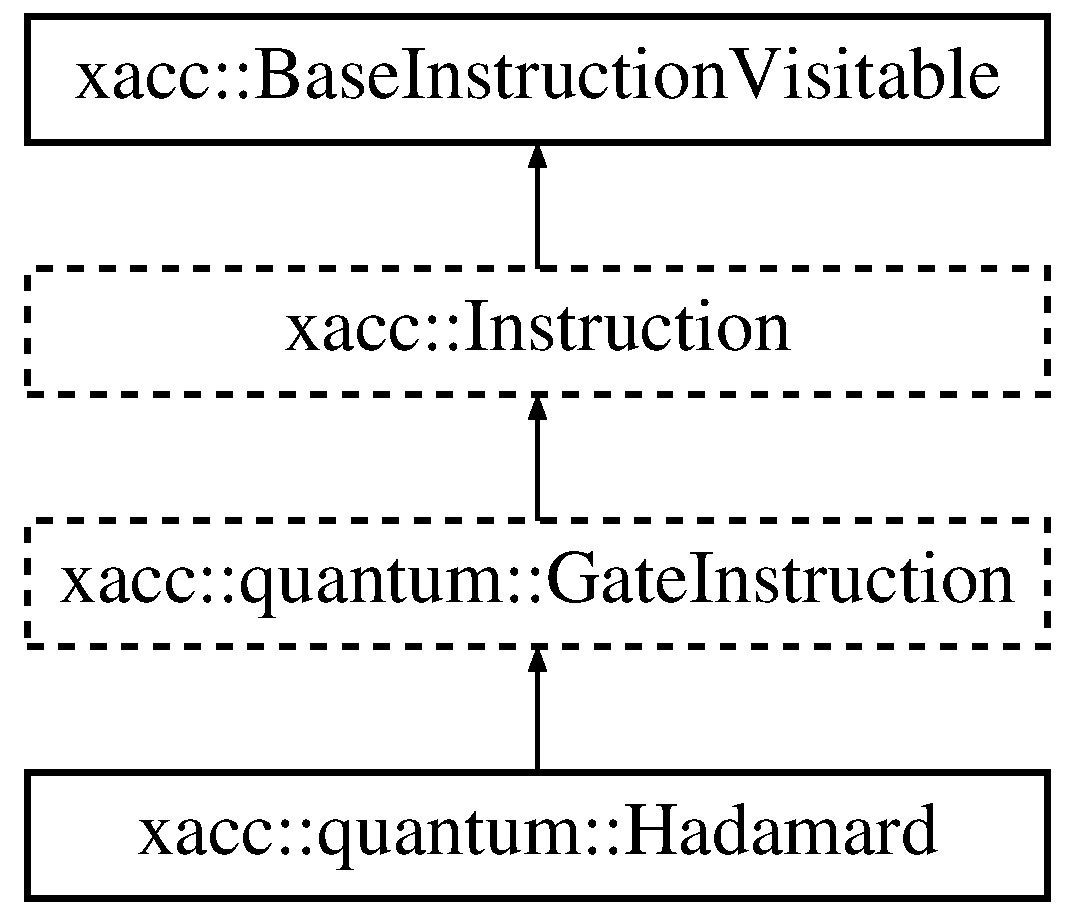
\includegraphics[height=4.000000cm]{a01187}
\end{center}
\end{figure}
\subsection*{Public Member Functions}
\begin{DoxyCompactItemize}
\item 
\mbox{\Hypertarget{a01187_a1f26925eeb4a52ca7e52dd9158fe7005}\label{a01187_a1f26925eeb4a52ca7e52dd9158fe7005}} 
{\bfseries Hadamard} (std\+::vector$<$ int $>$ \hyperlink{a01159_a2a56be6c2519ea65df4d06f4abae1393}{qbits})
\item 
\mbox{\Hypertarget{a01187_aac4e06aae35583bcce39b6b178948364}\label{a01187_aac4e06aae35583bcce39b6b178948364}} 
{\bfseries Hadamard} (int qbit)
\end{DoxyCompactItemize}
\subsection*{Additional Inherited Members}


The documentation for this class was generated from the following files\+:\begin{DoxyCompactItemize}
\item 
Hadamard.\+hpp\item 
Hadamard.\+cpp\end{DoxyCompactItemize}

\hypertarget{a01275}{}\section{fire\+:\+:I\+Local\+Parser$<$ T $>$ Class Template Reference}
\label{a01275}\index{fire\+::\+I\+Local\+Parser$<$ T $>$@{fire\+::\+I\+Local\+Parser$<$ T $>$}}


{\ttfamily \#include $<$I\+Local\+Parser.\+h$>$}

Inheritance diagram for fire\+:\+:I\+Local\+Parser$<$ T $>$\+:\begin{figure}[H]
\begin{center}
\leavevmode
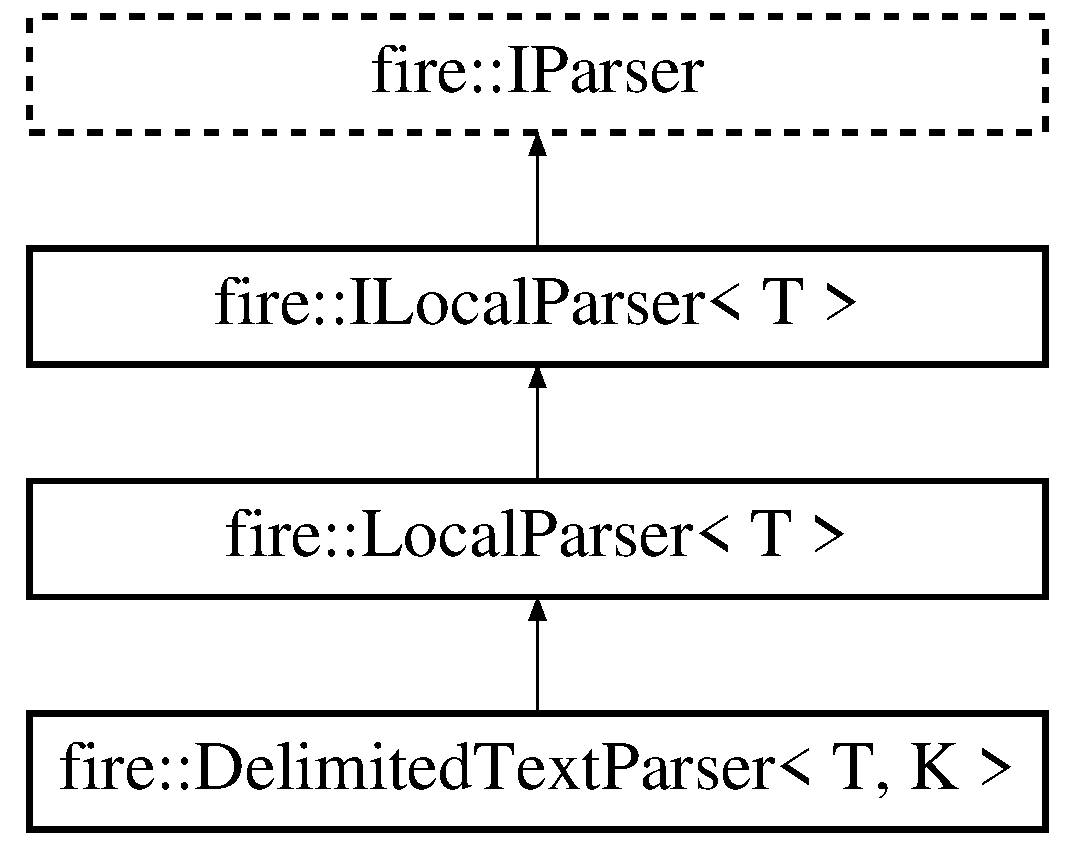
\includegraphics[height=4.000000cm]{a01275}
\end{center}
\end{figure}
\subsection*{Public Member Functions}
\begin{DoxyCompactItemize}
\item 
virtual bool \hyperlink{a01275_a091d5cf56bf8f407854ef87f460b2958}{is\+File} ()
\item 
virtual bool \hyperlink{a01275_a770acae6e216de3a9c7140a12de25d58}{is\+Local} ()
\item 
virtual bool \hyperlink{a01275_ad46898c516adcce38acbb4800dc9777b}{is\+Parallel} ()
\item 
virtual std\+::shared\+\_\+ptr$<$ T $>$ \hyperlink{a01275_a0fc1446d106f0ab8daf8744a4bd29a65}{get\+Data} ()=0
\end{DoxyCompactItemize}
\subsection*{Protected Attributes}
\begin{DoxyCompactItemize}
\item 
bool \hyperlink{a01275_a39adf288ae0bc79cf39fd6e4638858cf}{is\+A\+File} = true
\end{DoxyCompactItemize}


\subsection{Detailed Description}
\subsubsection*{template$<$typename T$>$\newline
class fire\+::\+I\+Local\+Parser$<$ T $>$}

This is a sub-\/interface of \hyperlink{a01283}{I\+Parser} that represents a parser for a local, serially executed parser.

\hyperlink{a01275_a770acae6e216de3a9c7140a12de25d58}{is\+Local()} always returns true. \hyperlink{a01275_ad46898c516adcce38acbb4800dc9777b}{is\+Parallel()} always returns false.

Implementations should set is\+File in their set\+Source(std\+::string) if their source is a file. Subclasses must always be sure that they implement \hyperlink{a01283_af36ac6eedd8c27d2f418869193d7d03c}{parse()} and \hyperlink{a01283_a0dbeff2b9bd8dbfb2aad7a424eef87d1}{set\+Source()} because default implementations are not provided.

The \hyperlink{a01275_a0fc1446d106f0ab8daf8744a4bd29a65}{get\+Data()} operation always returns a shared\+\_\+ptr instead of a raw type (copy) or raw pointer to efficiently share the dynamically allocated data. 

\subsection{Member Function Documentation}
\mbox{\Hypertarget{a01275_a0fc1446d106f0ab8daf8744a4bd29a65}\label{a01275_a0fc1446d106f0ab8daf8744a4bd29a65}} 
\index{fire\+::\+I\+Local\+Parser@{fire\+::\+I\+Local\+Parser}!get\+Data@{get\+Data}}
\index{get\+Data@{get\+Data}!fire\+::\+I\+Local\+Parser@{fire\+::\+I\+Local\+Parser}}
\subsubsection{\texorpdfstring{get\+Data()}{getData()}}
{\footnotesize\ttfamily template$<$typename T$>$ \\
virtual std\+::shared\+\_\+ptr$<$T$>$ \hyperlink{a01275}{fire\+::\+I\+Local\+Parser}$<$ T $>$\+::get\+Data (\begin{DoxyParamCaption}{ }\end{DoxyParamCaption})\hspace{0.3cm}{\ttfamily [pure virtual]}}

This operation returns a shared pointer to an instance of type T. \begin{DoxyReturn}{Returns}
a shared pointer holding an instance of type T that was parsed from the file. 
\end{DoxyReturn}


Implemented in \hyperlink{a01291_ab9016cca8e5dca516bb57c6a8e76607a}{fire\+::\+Local\+Parser$<$ T $>$}, and \hyperlink{a01291_ab9016cca8e5dca516bb57c6a8e76607a}{fire\+::\+Local\+Parser$<$ std\+::string $>$}.

\mbox{\Hypertarget{a01275_a091d5cf56bf8f407854ef87f460b2958}\label{a01275_a091d5cf56bf8f407854ef87f460b2958}} 
\index{fire\+::\+I\+Local\+Parser@{fire\+::\+I\+Local\+Parser}!is\+File@{is\+File}}
\index{is\+File@{is\+File}!fire\+::\+I\+Local\+Parser@{fire\+::\+I\+Local\+Parser}}
\subsubsection{\texorpdfstring{is\+File()}{isFile()}}
{\footnotesize\ttfamily template$<$typename T$>$ \\
virtual bool \hyperlink{a01275}{fire\+::\+I\+Local\+Parser}$<$ T $>$\+::is\+File (\begin{DoxyParamCaption}{ }\end{DoxyParamCaption})\hspace{0.3cm}{\ttfamily [inline]}, {\ttfamily [virtual]}}

This operation indicates whether or not the parser\textquotesingle{}s source is a file. \begin{DoxyReturn}{Returns}
true if this parser is working with a file, false otherwise. 
\end{DoxyReturn}


Implements \hyperlink{a01283_a616c42c85d781c916e97f0ad8f1e9010}{fire\+::\+I\+Parser}.

\mbox{\Hypertarget{a01275_a770acae6e216de3a9c7140a12de25d58}\label{a01275_a770acae6e216de3a9c7140a12de25d58}} 
\index{fire\+::\+I\+Local\+Parser@{fire\+::\+I\+Local\+Parser}!is\+Local@{is\+Local}}
\index{is\+Local@{is\+Local}!fire\+::\+I\+Local\+Parser@{fire\+::\+I\+Local\+Parser}}
\subsubsection{\texorpdfstring{is\+Local()}{isLocal()}}
{\footnotesize\ttfamily template$<$typename T$>$ \\
virtual bool \hyperlink{a01275}{fire\+::\+I\+Local\+Parser}$<$ T $>$\+::is\+Local (\begin{DoxyParamCaption}{ }\end{DoxyParamCaption})\hspace{0.3cm}{\ttfamily [inline]}, {\ttfamily [virtual]}}

This operation indicates whether or not the parser is using a local source. \begin{DoxyReturn}{Returns}
true if this parser is working with a local source, false otherwise. 
\end{DoxyReturn}


Implements \hyperlink{a01283_a97b9e58493b3cadbc63e670b0b0e759f}{fire\+::\+I\+Parser}.

\mbox{\Hypertarget{a01275_ad46898c516adcce38acbb4800dc9777b}\label{a01275_ad46898c516adcce38acbb4800dc9777b}} 
\index{fire\+::\+I\+Local\+Parser@{fire\+::\+I\+Local\+Parser}!is\+Parallel@{is\+Parallel}}
\index{is\+Parallel@{is\+Parallel}!fire\+::\+I\+Local\+Parser@{fire\+::\+I\+Local\+Parser}}
\subsubsection{\texorpdfstring{is\+Parallel()}{isParallel()}}
{\footnotesize\ttfamily template$<$typename T$>$ \\
virtual bool \hyperlink{a01275}{fire\+::\+I\+Local\+Parser}$<$ T $>$\+::is\+Parallel (\begin{DoxyParamCaption}{ }\end{DoxyParamCaption})\hspace{0.3cm}{\ttfamily [inline]}, {\ttfamily [virtual]}}

This operation indicates whether or not the parser reads in parallel. \begin{DoxyReturn}{Returns}
true if this parser reads in parallel, false otherwise. 
\end{DoxyReturn}


Implements \hyperlink{a01283_a83d2882a466d694fb0aea3d846bcbed4}{fire\+::\+I\+Parser}.



\subsection{Member Data Documentation}
\mbox{\Hypertarget{a01275_a39adf288ae0bc79cf39fd6e4638858cf}\label{a01275_a39adf288ae0bc79cf39fd6e4638858cf}} 
\index{fire\+::\+I\+Local\+Parser@{fire\+::\+I\+Local\+Parser}!is\+A\+File@{is\+A\+File}}
\index{is\+A\+File@{is\+A\+File}!fire\+::\+I\+Local\+Parser@{fire\+::\+I\+Local\+Parser}}
\subsubsection{\texorpdfstring{is\+A\+File}{isAFile}}
{\footnotesize\ttfamily template$<$typename T$>$ \\
bool \hyperlink{a01275}{fire\+::\+I\+Local\+Parser}$<$ T $>$\+::is\+A\+File = true\hspace{0.3cm}{\ttfamily [protected]}}

This value is true if the source is a file and false if it is a stream. This value should be set in the set\+Source(std\+::string) and set\+Source(std\+::istream) to true and false respectively. It is set to true by default. 

The documentation for this class was generated from the following file\+:\begin{DoxyCompactItemize}
\item 
I\+Local\+Parser.\+h\end{DoxyCompactItemize}

\hypertarget{a01279}{}\section{fire\+:\+:I\+N\+I\+Property\+Parser Class Reference}
\label{a01279}\index{fire\+::\+I\+N\+I\+Property\+Parser@{fire\+::\+I\+N\+I\+Property\+Parser}}


{\ttfamily \#include $<$I\+N\+I\+Property\+Parser.\+h$>$}

Inheritance diagram for fire\+:\+:I\+N\+I\+Property\+Parser\+:\begin{figure}[H]
\begin{center}
\leavevmode
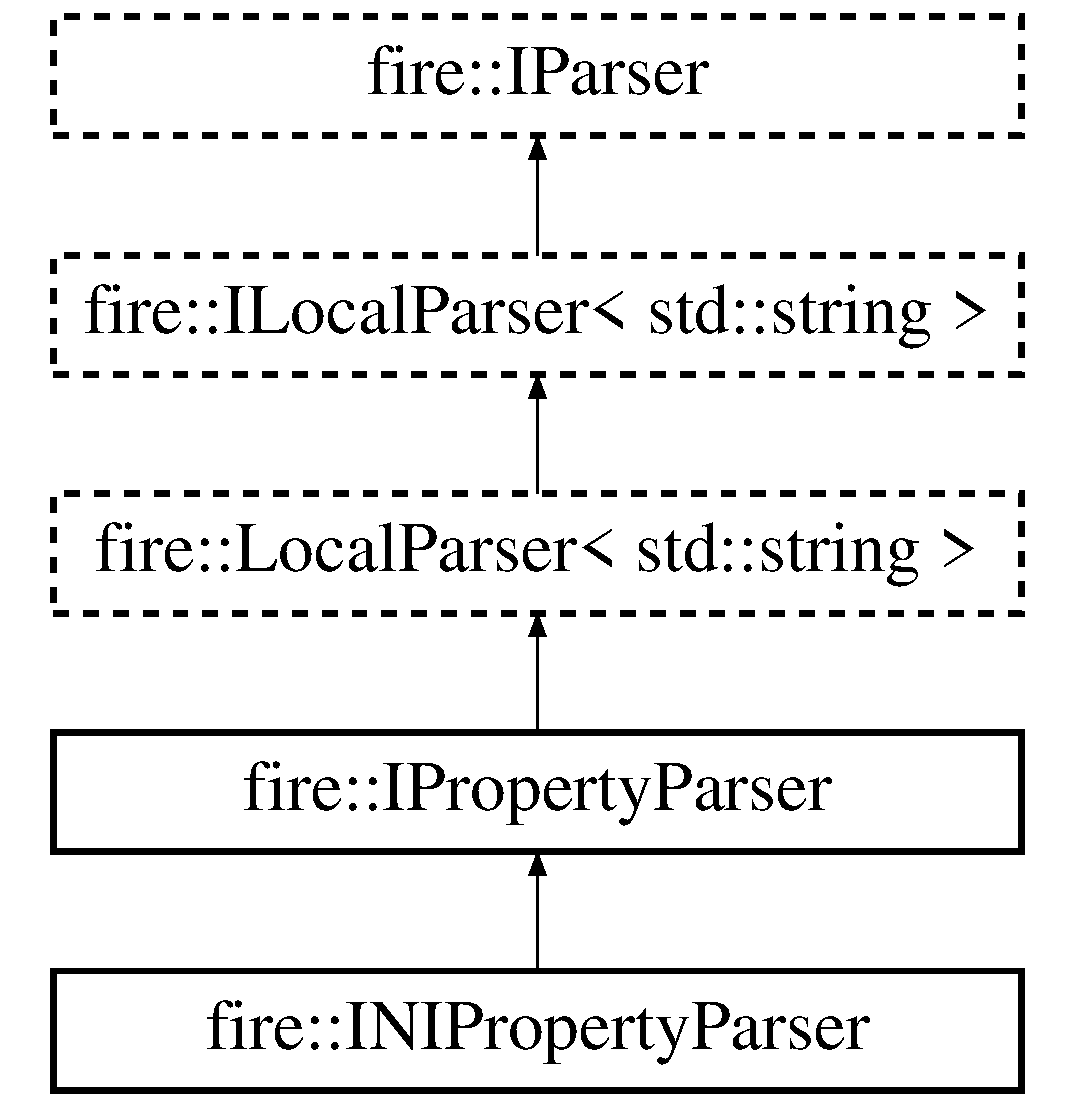
\includegraphics[height=5.000000cm]{a01279}
\end{center}
\end{figure}
\subsection*{Public Member Functions}
\begin{DoxyCompactItemize}
\item 
virtual void \hyperlink{a01279_a06793909bc707a69d0c5772b14bc946d}{set\+Source} (const std\+::string \&source)
\item 
virtual const std\+::string \& \hyperlink{a01279_ad02c9a530f20a706d7bb2554813e8d3a}{get\+Source} ()
\item 
virtual void \hyperlink{a01279_a31b6bad01e65ed4bb5f1ba297616c641}{parse} ()
\item 
virtual const std\+::vector$<$ std\+::string $>$ \& \hyperlink{a01279_aed0f1f47111794659564dcddb4d25bc6}{get\+Property\+Block\+Names} ()
\item 
virtual const std\+::map$<$ std\+::string, std\+::string $>$ \& \hyperlink{a01279_a3591312590a66659ebd377cdde9ab9ad}{get\+Property\+Block} (const std\+::string \&name)
\end{DoxyCompactItemize}
\subsection*{Additional Inherited Members}


\subsection{Detailed Description}
This class implements \hyperlink{a01287}{I\+Property\+Parser} to provide a local, file-\/based, serially executed I\+NI parser.

\hyperlink{a01275_a091d5cf56bf8f407854ef87f460b2958}{is\+File()} always returns true. \hyperlink{a01275_a770acae6e216de3a9c7140a12de25d58}{is\+Local()} always returns true. \hyperlink{a01275_ad46898c516adcce38acbb4800dc9777b}{is\+Parallel()} always returns false.

This implementation is backed by Simple\+I\+NI, one of Fire\textquotesingle{}s dependencies, so it supports whatever Simple\+I\+NI supports.

The source must be a file on the local filesystem. 

\subsection{Member Function Documentation}
\mbox{\Hypertarget{a01279_a3591312590a66659ebd377cdde9ab9ad}\label{a01279_a3591312590a66659ebd377cdde9ab9ad}} 
\index{fire\+::\+I\+N\+I\+Property\+Parser@{fire\+::\+I\+N\+I\+Property\+Parser}!get\+Property\+Block@{get\+Property\+Block}}
\index{get\+Property\+Block@{get\+Property\+Block}!fire\+::\+I\+N\+I\+Property\+Parser@{fire\+::\+I\+N\+I\+Property\+Parser}}
\subsubsection{\texorpdfstring{get\+Property\+Block()}{getPropertyBlock()}}
{\footnotesize\ttfamily virtual const std\+::map$<$std\+::string, std\+::string$>$\& fire\+::\+I\+N\+I\+Property\+Parser\+::get\+Property\+Block (\begin{DoxyParamCaption}\item[{const std\+::string \&}]{name }\end{DoxyParamCaption})\hspace{0.3cm}{\ttfamily [inline]}, {\ttfamily [virtual]}}

This operation returns the property block with the given name. 
\begin{DoxyParams}{Parameters}
{\em name} & the block name \\
\hline
\end{DoxyParams}
\begin{DoxyReturn}{Returns}
the property block with the given name 
\end{DoxyReturn}


Implements \hyperlink{a01287_a34201371cb36dd09e96a66242ececb86}{fire\+::\+I\+Property\+Parser}.

\mbox{\Hypertarget{a01279_aed0f1f47111794659564dcddb4d25bc6}\label{a01279_aed0f1f47111794659564dcddb4d25bc6}} 
\index{fire\+::\+I\+N\+I\+Property\+Parser@{fire\+::\+I\+N\+I\+Property\+Parser}!get\+Property\+Block\+Names@{get\+Property\+Block\+Names}}
\index{get\+Property\+Block\+Names@{get\+Property\+Block\+Names}!fire\+::\+I\+N\+I\+Property\+Parser@{fire\+::\+I\+N\+I\+Property\+Parser}}
\subsubsection{\texorpdfstring{get\+Property\+Block\+Names()}{getPropertyBlockNames()}}
{\footnotesize\ttfamily virtual const std\+::vector$<$std\+::string$>$\& fire\+::\+I\+N\+I\+Property\+Parser\+::get\+Property\+Block\+Names (\begin{DoxyParamCaption}{ }\end{DoxyParamCaption})\hspace{0.3cm}{\ttfamily [inline]}, {\ttfamily [virtual]}}

This operation returns the names of the property blocks parsed from the source. \begin{DoxyReturn}{Returns}
the block names 
\end{DoxyReturn}


Implements \hyperlink{a01287_a34602687f9d1affac7bd842102d4a6aa}{fire\+::\+I\+Property\+Parser}.

\mbox{\Hypertarget{a01279_ad02c9a530f20a706d7bb2554813e8d3a}\label{a01279_ad02c9a530f20a706d7bb2554813e8d3a}} 
\index{fire\+::\+I\+N\+I\+Property\+Parser@{fire\+::\+I\+N\+I\+Property\+Parser}!get\+Source@{get\+Source}}
\index{get\+Source@{get\+Source}!fire\+::\+I\+N\+I\+Property\+Parser@{fire\+::\+I\+N\+I\+Property\+Parser}}
\subsubsection{\texorpdfstring{get\+Source()}{getSource()}}
{\footnotesize\ttfamily virtual const std\+::string\& fire\+::\+I\+N\+I\+Property\+Parser\+::get\+Source (\begin{DoxyParamCaption}{ }\end{DoxyParamCaption})\hspace{0.3cm}{\ttfamily [inline]}, {\ttfamily [virtual]}}

This operation gets the data source for the parser. \begin{DoxyReturn}{Returns}
the name of the source 
\end{DoxyReturn}


Reimplemented from \hyperlink{a01291_aedb7fe10911182525a719963b9b56726}{fire\+::\+Local\+Parser$<$ std\+::string $>$}.

\mbox{\Hypertarget{a01279_a31b6bad01e65ed4bb5f1ba297616c641}\label{a01279_a31b6bad01e65ed4bb5f1ba297616c641}} 
\index{fire\+::\+I\+N\+I\+Property\+Parser@{fire\+::\+I\+N\+I\+Property\+Parser}!parse@{parse}}
\index{parse@{parse}!fire\+::\+I\+N\+I\+Property\+Parser@{fire\+::\+I\+N\+I\+Property\+Parser}}
\subsubsection{\texorpdfstring{parse()}{parse()}}
{\footnotesize\ttfamily virtual void fire\+::\+I\+N\+I\+Property\+Parser\+::parse (\begin{DoxyParamCaption}{ }\end{DoxyParamCaption})\hspace{0.3cm}{\ttfamily [inline]}, {\ttfamily [virtual]}}

This operation directs the parser to parse its source. 

Reimplemented from \hyperlink{a01291_abd8929aea06c2dda40256d2e58236650}{fire\+::\+Local\+Parser$<$ std\+::string $>$}.

\mbox{\Hypertarget{a01279_a06793909bc707a69d0c5772b14bc946d}\label{a01279_a06793909bc707a69d0c5772b14bc946d}} 
\index{fire\+::\+I\+N\+I\+Property\+Parser@{fire\+::\+I\+N\+I\+Property\+Parser}!set\+Source@{set\+Source}}
\index{set\+Source@{set\+Source}!fire\+::\+I\+N\+I\+Property\+Parser@{fire\+::\+I\+N\+I\+Property\+Parser}}
\subsubsection{\texorpdfstring{set\+Source()}{setSource()}}
{\footnotesize\ttfamily virtual void fire\+::\+I\+N\+I\+Property\+Parser\+::set\+Source (\begin{DoxyParamCaption}\item[{const std\+::string \&}]{source }\end{DoxyParamCaption})\hspace{0.3cm}{\ttfamily [inline]}, {\ttfamily [virtual]}}

This operation sets the data source for the parser. 
\begin{DoxyParams}{Parameters}
{\em source} & the name of the source that the parser should parse. \\
\hline
\end{DoxyParams}


Reimplemented from \hyperlink{a01291_afcaec6429fdd6e5d53642a32c001ff73}{fire\+::\+Local\+Parser$<$ std\+::string $>$}.



The documentation for this class was generated from the following file\+:\begin{DoxyCompactItemize}
\item 
I\+N\+I\+Property\+Parser.\+h\end{DoxyCompactItemize}

\hypertarget{a01371}{}\section{fire\+:\+:Initializer$<$ Fire\+Tensor, Scalar, N $>$ Struct Template Reference}
\label{a01371}\index{fire\+::\+Initializer$<$ Fire\+Tensor, Scalar, N $>$@{fire\+::\+Initializer$<$ Fire\+Tensor, Scalar, N $>$}}


{\ttfamily \#include $<$Tensor\+Utils.\+hpp$>$}

\subsection*{Public Types}
\begin{DoxyCompactItemize}
\item 
\mbox{\Hypertarget{a01371_aeb5626b5276d5c021ba8971b2d524c45}\label{a01371_aeb5626b5276d5c021ba8971b2d524c45}} 
typedef std\+::initializer\+\_\+list$<$ typename \hyperlink{a01371}{Initializer}$<$ \hyperlink{a01347}{Fire\+Tensor}, Scalar, N -\/ 1 $>$\+::Init\+List $>$ {\bfseries Init\+List}
\end{DoxyCompactItemize}


\subsection{Detailed Description}
\subsubsection*{template$<$typename Fire\+Tensor, typename Scalar, int N$>$\newline
struct fire\+::\+Initializer$<$ Fire\+Tensor, Scalar, N $>$}

The following three templates set up the recursion necessary to express nexted std\+::initializer\+\_\+lists. We use this to accept tensor values and set them on the internal \hyperlink{a01351}{Tensor\+Provider} tensor instance. 

The documentation for this struct was generated from the following file\+:\begin{DoxyCompactItemize}
\item 
Tensor\+Utils.\+hpp\end{DoxyCompactItemize}

\hypertarget{a01379}{}\section{fire\+:\+:Initializer$<$ Fire\+Tensor, Scalar, 0 $>$ Struct Template Reference}
\label{a01379}\index{fire\+::\+Initializer$<$ Fire\+Tensor, Scalar, 0 $>$@{fire\+::\+Initializer$<$ Fire\+Tensor, Scalar, 0 $>$}}
\subsection*{Public Types}
\begin{DoxyCompactItemize}
\item 
\mbox{\Hypertarget{a01379_aa3aa3da5b7d98e209a2c8f87d5a8371d}\label{a01379_aa3aa3da5b7d98e209a2c8f87d5a8371d}} 
typedef Scalar {\bfseries Init\+List}
\end{DoxyCompactItemize}


The documentation for this struct was generated from the following file\+:\begin{DoxyCompactItemize}
\item 
Tensor\+Utils.\+hpp\end{DoxyCompactItemize}

\hypertarget{a01375}{}\section{fire\+:\+:Initializer$<$ Fire\+Tensor, Scalar, 1 $>$ Struct Template Reference}
\label{a01375}\index{fire\+::\+Initializer$<$ Fire\+Tensor, Scalar, 1 $>$@{fire\+::\+Initializer$<$ Fire\+Tensor, Scalar, 1 $>$}}
\subsection*{Public Types}
\begin{DoxyCompactItemize}
\item 
\mbox{\Hypertarget{a01375_ab08b58675de0070598ae477a509856c8}\label{a01375_ab08b58675de0070598ae477a509856c8}} 
typedef std\+::initializer\+\_\+list$<$ Scalar $>$ {\bfseries Init\+List}
\end{DoxyCompactItemize}


The documentation for this struct was generated from the following file\+:\begin{DoxyCompactItemize}
\item 
Tensor\+Utils.\+hpp\end{DoxyCompactItemize}

\hypertarget{a01479}{}\section{xacc\+:\+:Instruction Class Reference}
\label{a01479}\index{xacc\+::\+Instruction@{xacc\+::\+Instruction}}


{\ttfamily \#include $<$Instruction.\+hpp$>$}

Inheritance diagram for xacc\+:\+:Instruction\+:\begin{figure}[H]
\begin{center}
\leavevmode
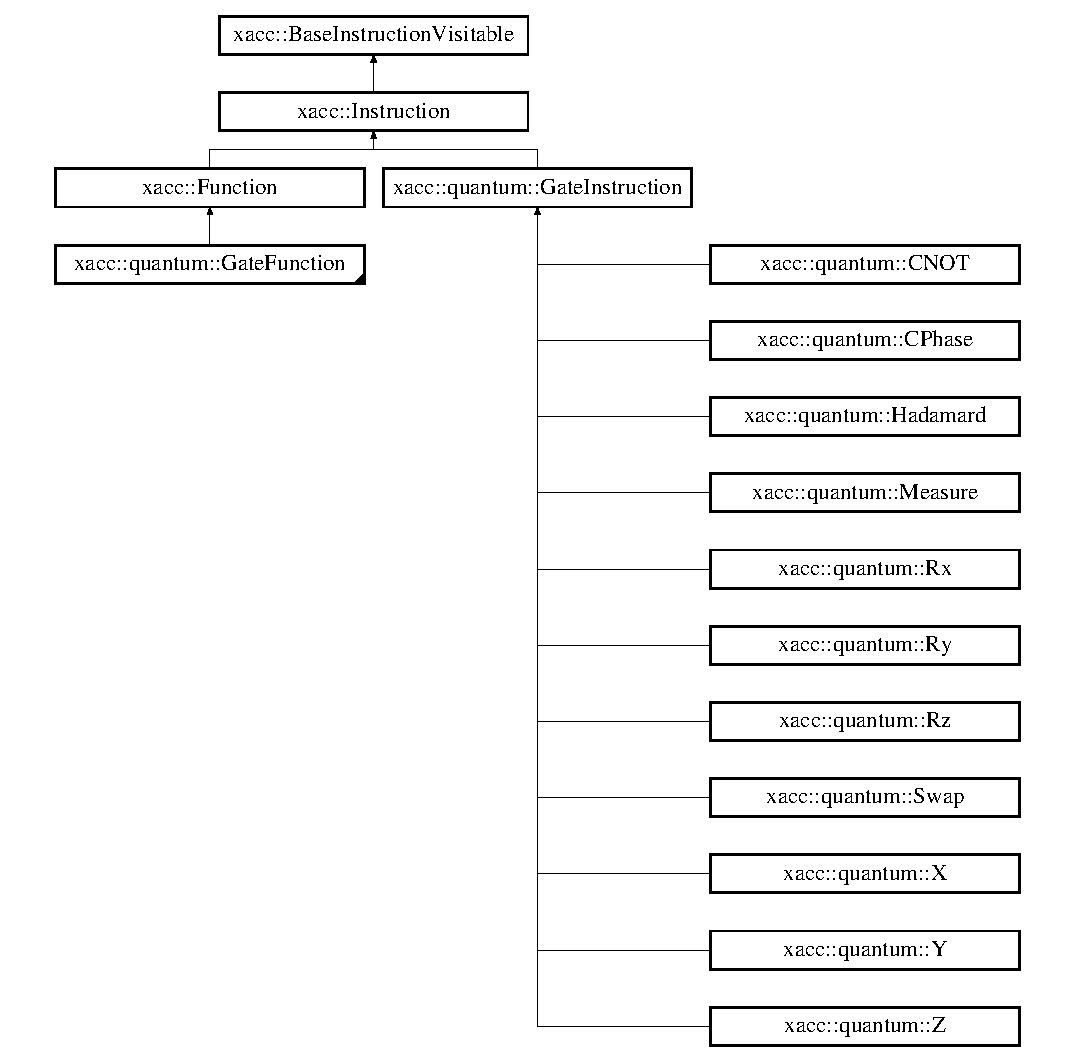
\includegraphics[height=12.000000cm]{a01479}
\end{center}
\end{figure}
\subsection*{Public Member Functions}
\begin{DoxyCompactItemize}
\item 
virtual const std\+::string \hyperlink{a01479_ac7ff23f693e2276edbf3fdac5452792c}{get\+Name} ()=0
\item 
virtual const std\+::string \hyperlink{a01479_ae94c2d089908294c1d410b14c96817ae}{to\+String} (const std\+::string \&buffer\+Var\+Name)=0
\item 
virtual const std\+::vector$<$ int $>$ \hyperlink{a01479_a819f32e94c3e1c9e69a0061aaf8d86dc}{bits} ()=0
\item 
virtual Instruction\+Parameter \hyperlink{a01479_aa0d9de97a4833a042379647f83c33ab6}{get\+Parameter} (const int idx)=0
\item 
virtual std\+::vector$<$ Instruction\+Parameter $>$ \hyperlink{a01479_aeb67c67713896e8f27a5c7dd531f3340}{get\+Parameters} ()=0
\item 
virtual void \hyperlink{a01479_a407a0ac662fa0b1ec3e301e8ff9bade7}{set\+Parameter} (const int idx, Instruction\+Parameter \&isnt)=0
\item 
virtual const int \hyperlink{a01479_ad54585d13c04ffd20296fff7ab8107ff}{n\+Parameters} ()=0
\item 
virtual bool \hyperlink{a01479_a7b24d8ae485369fc2b2df7a3224a5e26}{is\+Parameterized} ()
\item 
virtual bool \hyperlink{a01479_a4383f1036d0fcfe890ab9c613dbd5f38}{is\+Composite} ()
\item 
virtual bool \hyperlink{a01479_ad02a1cf7220577124720b7a51424cea7}{is\+Enabled} ()
\item 
virtual void \hyperlink{a01479_a6e528da15e05a94cc1d7db268c483271}{disable} ()
\item 
virtual void \hyperlink{a01479_a0b4f2e5a591af28342a3c08e4305e24f}{enable} ()
\item 
virtual \hyperlink{a01479_ae22c935e8113bce63d1d0e214cda4d61}{$\sim$\+Instruction} ()
\end{DoxyCompactItemize}
\subsection*{Additional Inherited Members}


\subsection{Detailed Description}
The \hyperlink{a01479}{Instruction} interface is the base of all X\+A\+CC Intermediate Representation Instructions for post-\/\+Moore\textquotesingle{}s law accelerated computing. The \hyperlink{a01479}{Instruction}, at its core, provides an \hyperlink{a01479}{Instruction} name and a set of next-\/gen bits that the \hyperlink{a01479}{Instruction} operates on. Instructions can also be enabled or disabled. Instructions implement \hyperlink{a01495}{Base\+Instruction\+Visitable} to enable visitor pattern functionality across all \hyperlink{a01479}{Instruction} subclasses.

\hyperlink{a01479}{Instruction} can also expose 0 to N Instruction\+Parameters. Instruction\+Parameters can be an int, double, float, or string. 

\subsection{Constructor \& Destructor Documentation}
\mbox{\Hypertarget{a01479_ae22c935e8113bce63d1d0e214cda4d61}\label{a01479_ae22c935e8113bce63d1d0e214cda4d61}} 
\index{xacc\+::\+Instruction@{xacc\+::\+Instruction}!````~Instruction@{$\sim$\+Instruction}}
\index{````~Instruction@{$\sim$\+Instruction}!xacc\+::\+Instruction@{xacc\+::\+Instruction}}
\subsubsection{\texorpdfstring{$\sim$\+Instruction()}{~Instruction()}}
{\footnotesize\ttfamily virtual xacc\+::\+Instruction\+::$\sim$\+Instruction (\begin{DoxyParamCaption}{ }\end{DoxyParamCaption})\hspace{0.3cm}{\ttfamily [inline]}, {\ttfamily [virtual]}}

The destructor 

\subsection{Member Function Documentation}
\mbox{\Hypertarget{a01479_a819f32e94c3e1c9e69a0061aaf8d86dc}\label{a01479_a819f32e94c3e1c9e69a0061aaf8d86dc}} 
\index{xacc\+::\+Instruction@{xacc\+::\+Instruction}!bits@{bits}}
\index{bits@{bits}!xacc\+::\+Instruction@{xacc\+::\+Instruction}}
\subsubsection{\texorpdfstring{bits()}{bits()}}
{\footnotesize\ttfamily virtual const std\+::vector$<$int$>$ xacc\+::\+Instruction\+::bits (\begin{DoxyParamCaption}{ }\end{DoxyParamCaption})\hspace{0.3cm}{\ttfamily [pure virtual]}}

Return the indices of the bits that this \hyperlink{a01479}{Instruction} operates on.

\begin{DoxyReturn}{Returns}
bits The bits this \hyperlink{a01479}{Instruction} operates on. 
\end{DoxyReturn}


Implemented in \hyperlink{a01155_aba03de68b76a9e120705c3c389c714a1}{xacc\+::quantum\+::\+Gate\+Function}, and \hyperlink{a01159_ad32ad03dfc516e00093030e60178003d}{xacc\+::quantum\+::\+Gate\+Instruction}.

\mbox{\Hypertarget{a01479_a6e528da15e05a94cc1d7db268c483271}\label{a01479_a6e528da15e05a94cc1d7db268c483271}} 
\index{xacc\+::\+Instruction@{xacc\+::\+Instruction}!disable@{disable}}
\index{disable@{disable}!xacc\+::\+Instruction@{xacc\+::\+Instruction}}
\subsubsection{\texorpdfstring{disable()}{disable()}}
{\footnotesize\ttfamily virtual void xacc\+::\+Instruction\+::disable (\begin{DoxyParamCaption}{ }\end{DoxyParamCaption})\hspace{0.3cm}{\ttfamily [inline]}, {\ttfamily [virtual]}}

Disable this \hyperlink{a01479}{Instruction} 

Reimplemented in \hyperlink{a01159_a63ce138dd71fb43d303f5600fefb7215}{xacc\+::quantum\+::\+Gate\+Instruction}.

\mbox{\Hypertarget{a01479_a0b4f2e5a591af28342a3c08e4305e24f}\label{a01479_a0b4f2e5a591af28342a3c08e4305e24f}} 
\index{xacc\+::\+Instruction@{xacc\+::\+Instruction}!enable@{enable}}
\index{enable@{enable}!xacc\+::\+Instruction@{xacc\+::\+Instruction}}
\subsubsection{\texorpdfstring{enable()}{enable()}}
{\footnotesize\ttfamily virtual void xacc\+::\+Instruction\+::enable (\begin{DoxyParamCaption}{ }\end{DoxyParamCaption})\hspace{0.3cm}{\ttfamily [inline]}, {\ttfamily [virtual]}}

Enable this \hyperlink{a01479}{Instruction}. 

Reimplemented in \hyperlink{a01159_a7a80474b7fd465271b3313432db2e608}{xacc\+::quantum\+::\+Gate\+Instruction}.

\mbox{\Hypertarget{a01479_ac7ff23f693e2276edbf3fdac5452792c}\label{a01479_ac7ff23f693e2276edbf3fdac5452792c}} 
\index{xacc\+::\+Instruction@{xacc\+::\+Instruction}!get\+Name@{get\+Name}}
\index{get\+Name@{get\+Name}!xacc\+::\+Instruction@{xacc\+::\+Instruction}}
\subsubsection{\texorpdfstring{get\+Name()}{getName()}}
{\footnotesize\ttfamily virtual const std\+::string xacc\+::\+Instruction\+::get\+Name (\begin{DoxyParamCaption}{ }\end{DoxyParamCaption})\hspace{0.3cm}{\ttfamily [pure virtual]}}

Return the name of this \hyperlink{a01479}{Instruction}

\begin{DoxyReturn}{Returns}
name The name of this \hyperlink{a01479}{Instruction} 
\end{DoxyReturn}


Implemented in \hyperlink{a01155_af42efb6191267164717d53c469e15d3a}{xacc\+::quantum\+::\+Gate\+Function}, and \hyperlink{a01159_a0db03b9e46eeba1134f0ca2b83ccc842}{xacc\+::quantum\+::\+Gate\+Instruction}.

\mbox{\Hypertarget{a01479_aa0d9de97a4833a042379647f83c33ab6}\label{a01479_aa0d9de97a4833a042379647f83c33ab6}} 
\index{xacc\+::\+Instruction@{xacc\+::\+Instruction}!get\+Parameter@{get\+Parameter}}
\index{get\+Parameter@{get\+Parameter}!xacc\+::\+Instruction@{xacc\+::\+Instruction}}
\subsubsection{\texorpdfstring{get\+Parameter()}{getParameter()}}
{\footnotesize\ttfamily virtual Instruction\+Parameter xacc\+::\+Instruction\+::get\+Parameter (\begin{DoxyParamCaption}\item[{const int}]{idx }\end{DoxyParamCaption})\hspace{0.3cm}{\ttfamily [pure virtual]}}

Return this \hyperlink{a01479}{Instruction}\textquotesingle{}s parameter at the given index.


\begin{DoxyParams}{Parameters}
{\em idx} & The index of the parameter. \\
\hline
\end{DoxyParams}
\begin{DoxyReturn}{Returns}
param The Instruction\+Parameter at the given index. 
\end{DoxyReturn}


Implemented in \hyperlink{a01155_a5991903323e412777bedc4f0c862eb63}{xacc\+::quantum\+::\+Gate\+Function}, and \hyperlink{a01159_addd6185279fe99fbdc3d4efd96e42162}{xacc\+::quantum\+::\+Gate\+Instruction}.

\mbox{\Hypertarget{a01479_aeb67c67713896e8f27a5c7dd531f3340}\label{a01479_aeb67c67713896e8f27a5c7dd531f3340}} 
\index{xacc\+::\+Instruction@{xacc\+::\+Instruction}!get\+Parameters@{get\+Parameters}}
\index{get\+Parameters@{get\+Parameters}!xacc\+::\+Instruction@{xacc\+::\+Instruction}}
\subsubsection{\texorpdfstring{get\+Parameters()}{getParameters()}}
{\footnotesize\ttfamily virtual std\+::vector$<$Instruction\+Parameter$>$ xacc\+::\+Instruction\+::get\+Parameters (\begin{DoxyParamCaption}{ }\end{DoxyParamCaption})\hspace{0.3cm}{\ttfamily [pure virtual]}}

Return all of this \hyperlink{a01479}{Instruction}\textquotesingle{}s parameters.

\begin{DoxyReturn}{Returns}
params This instructions parameters. 
\end{DoxyReturn}


Implemented in \hyperlink{a01155_af7aabfe699a4dced576ff7fafff969d5}{xacc\+::quantum\+::\+Gate\+Function}, and \hyperlink{a01159_a8584444f9577283f6844ab32bdc4db72}{xacc\+::quantum\+::\+Gate\+Instruction}.

\mbox{\Hypertarget{a01479_a4383f1036d0fcfe890ab9c613dbd5f38}\label{a01479_a4383f1036d0fcfe890ab9c613dbd5f38}} 
\index{xacc\+::\+Instruction@{xacc\+::\+Instruction}!is\+Composite@{is\+Composite}}
\index{is\+Composite@{is\+Composite}!xacc\+::\+Instruction@{xacc\+::\+Instruction}}
\subsubsection{\texorpdfstring{is\+Composite()}{isComposite()}}
{\footnotesize\ttfamily virtual bool xacc\+::\+Instruction\+::is\+Composite (\begin{DoxyParamCaption}{ }\end{DoxyParamCaption})\hspace{0.3cm}{\ttfamily [inline]}, {\ttfamily [virtual]}}

Returns true if this \hyperlink{a01479}{Instruction} is composite, ie, contains other Instructions.

\begin{DoxyReturn}{Returns}
is\+Composite True if this is a composite \hyperlink{a01479}{Instruction} 
\end{DoxyReturn}


Reimplemented in \hyperlink{a01475_aa75500c657b5c3e0e36213e1506aad97}{xacc\+::\+Function}.

\mbox{\Hypertarget{a01479_ad02a1cf7220577124720b7a51424cea7}\label{a01479_ad02a1cf7220577124720b7a51424cea7}} 
\index{xacc\+::\+Instruction@{xacc\+::\+Instruction}!is\+Enabled@{is\+Enabled}}
\index{is\+Enabled@{is\+Enabled}!xacc\+::\+Instruction@{xacc\+::\+Instruction}}
\subsubsection{\texorpdfstring{is\+Enabled()}{isEnabled()}}
{\footnotesize\ttfamily virtual bool xacc\+::\+Instruction\+::is\+Enabled (\begin{DoxyParamCaption}{ }\end{DoxyParamCaption})\hspace{0.3cm}{\ttfamily [inline]}, {\ttfamily [virtual]}}

Returns true if this \hyperlink{a01479}{Instruction} is enabled

\begin{DoxyReturn}{Returns}
enabled True if this \hyperlink{a01479}{Instruction} is enabled. 
\end{DoxyReturn}


Reimplemented in \hyperlink{a01159_a0a821be322b0c848b01c55f91fc8f484}{xacc\+::quantum\+::\+Gate\+Instruction}.

\mbox{\Hypertarget{a01479_a7b24d8ae485369fc2b2df7a3224a5e26}\label{a01479_a7b24d8ae485369fc2b2df7a3224a5e26}} 
\index{xacc\+::\+Instruction@{xacc\+::\+Instruction}!is\+Parameterized@{is\+Parameterized}}
\index{is\+Parameterized@{is\+Parameterized}!xacc\+::\+Instruction@{xacc\+::\+Instruction}}
\subsubsection{\texorpdfstring{is\+Parameterized()}{isParameterized()}}
{\footnotesize\ttfamily virtual bool xacc\+::\+Instruction\+::is\+Parameterized (\begin{DoxyParamCaption}{ }\end{DoxyParamCaption})\hspace{0.3cm}{\ttfamily [inline]}, {\ttfamily [virtual]}}

Return true if this \hyperlink{a01479}{Instruction} is parameterized.

\begin{DoxyReturn}{Returns}
parameterized True if this \hyperlink{a01479}{Instruction} has parameters. 
\end{DoxyReturn}


Reimplemented in \hyperlink{a01155_afad47903e0ed55ddbfa827ef8408a94b}{xacc\+::quantum\+::\+Gate\+Function}, and \hyperlink{a01159_afe7aeeb398262931e156bcb3950f8188}{xacc\+::quantum\+::\+Gate\+Instruction}.

\mbox{\Hypertarget{a01479_ad54585d13c04ffd20296fff7ab8107ff}\label{a01479_ad54585d13c04ffd20296fff7ab8107ff}} 
\index{xacc\+::\+Instruction@{xacc\+::\+Instruction}!n\+Parameters@{n\+Parameters}}
\index{n\+Parameters@{n\+Parameters}!xacc\+::\+Instruction@{xacc\+::\+Instruction}}
\subsubsection{\texorpdfstring{n\+Parameters()}{nParameters()}}
{\footnotesize\ttfamily virtual const int xacc\+::\+Instruction\+::n\+Parameters (\begin{DoxyParamCaption}{ }\end{DoxyParamCaption})\hspace{0.3cm}{\ttfamily [pure virtual]}}

Return the number of Instruction\+Parameters this \hyperlink{a01479}{Instruction} contains.

\begin{DoxyReturn}{Returns}
n\+Insts The number of instructions. 
\end{DoxyReturn}


Implemented in \hyperlink{a01155_ad0bffcbc0884d81d6bdddf55385fc6c9}{xacc\+::quantum\+::\+Gate\+Function}, and \hyperlink{a01159_a3752912b2c402668ca4814e21d4bbd26}{xacc\+::quantum\+::\+Gate\+Instruction}.

\mbox{\Hypertarget{a01479_a407a0ac662fa0b1ec3e301e8ff9bade7}\label{a01479_a407a0ac662fa0b1ec3e301e8ff9bade7}} 
\index{xacc\+::\+Instruction@{xacc\+::\+Instruction}!set\+Parameter@{set\+Parameter}}
\index{set\+Parameter@{set\+Parameter}!xacc\+::\+Instruction@{xacc\+::\+Instruction}}
\subsubsection{\texorpdfstring{set\+Parameter()}{setParameter()}}
{\footnotesize\ttfamily virtual void xacc\+::\+Instruction\+::set\+Parameter (\begin{DoxyParamCaption}\item[{const int}]{idx,  }\item[{Instruction\+Parameter \&}]{isnt }\end{DoxyParamCaption})\hspace{0.3cm}{\ttfamily [pure virtual]}}

Set this \hyperlink{a01479}{Instruction}\textquotesingle{}s parameter at the given index.


\begin{DoxyParams}{Parameters}
{\em idx} & The index of the parameter \\
\hline
{\em inst} & The instruction. \\
\hline
\end{DoxyParams}


Implemented in \hyperlink{a01155_ab8d9789b46e92e27a9d7c9c5b7e3683c}{xacc\+::quantum\+::\+Gate\+Function}, and \hyperlink{a01159_afb8f7582d7520c77d61b9016753f5669}{xacc\+::quantum\+::\+Gate\+Instruction}.

\mbox{\Hypertarget{a01479_ae94c2d089908294c1d410b14c96817ae}\label{a01479_ae94c2d089908294c1d410b14c96817ae}} 
\index{xacc\+::\+Instruction@{xacc\+::\+Instruction}!to\+String@{to\+String}}
\index{to\+String@{to\+String}!xacc\+::\+Instruction@{xacc\+::\+Instruction}}
\subsubsection{\texorpdfstring{to\+String()}{toString()}}
{\footnotesize\ttfamily virtual const std\+::string xacc\+::\+Instruction\+::to\+String (\begin{DoxyParamCaption}\item[{const std\+::string \&}]{buffer\+Var\+Name }\end{DoxyParamCaption})\hspace{0.3cm}{\ttfamily [pure virtual]}}

Persist this \hyperlink{a01479}{Instruction} to an assembly-\/like string.


\begin{DoxyParams}{Parameters}
{\em buffer\+Var\+Name} & The name of the \hyperlink{a01447}{Accelerator\+Buffer} \\
\hline
\end{DoxyParams}
\begin{DoxyReturn}{Returns}
str The assembly-\/like string. 
\end{DoxyReturn}


Implemented in \hyperlink{a01155_aa1950776ae84bad2d0795a0441f910e7}{xacc\+::quantum\+::\+Gate\+Function}, \hyperlink{a01159_a089a5da67ff40ac1a6f56e64589822d9}{xacc\+::quantum\+::\+Gate\+Instruction}, \hyperlink{a01191_a1c51a5d68294dcb2ba1a9fbea63a730f}{xacc\+::quantum\+::\+Measure}, and \hyperlink{a01179_aca7a5f849fece6fc28a904efee9a3370}{xacc\+::quantum\+::\+Conditional\+Function}.



The documentation for this class was generated from the following file\+:\begin{DoxyCompactItemize}
\item 
Instruction.\+hpp\end{DoxyCompactItemize}

\hypertarget{a01483}{}\section{xacc\+:\+:Instruction\+Iterator Class Reference}
\label{a01483}\index{xacc\+::\+Instruction\+Iterator@{xacc\+::\+Instruction\+Iterator}}


{\ttfamily \#include $<$Instruction\+Iterator.\+hpp$>$}

\subsection*{Public Member Functions}
\begin{DoxyCompactItemize}
\item 
\hyperlink{a01483_af61abf612341ab1454a1c43239b2da16}{Instruction\+Iterator} (std\+::shared\+\_\+ptr$<$ \hyperlink{a01479}{Instruction} $>$ r)
\item 
bool \hyperlink{a01483_a7fa6c8cff43e7b224211d4f7954a4152}{has\+Next} ()
\item 
std\+::shared\+\_\+ptr$<$ \hyperlink{a01479}{Instruction} $>$ \hyperlink{a01483_a0a2e2b1543650760a869460ebcd4382b}{next} ()
\end{DoxyCompactItemize}
\subsection*{Protected Attributes}
\begin{DoxyCompactItemize}
\item 
std\+::shared\+\_\+ptr$<$ \hyperlink{a01479}{Instruction} $>$ \hyperlink{a01483_a9d7aee1cb9058dd4a29c8fc71eeda57d}{root}
\item 
std\+::stack$<$ std\+::shared\+\_\+ptr$<$ \hyperlink{a01479}{Instruction} $>$ $>$ \hyperlink{a01483_a7af48509e563e8865131692c3b71edf0}{inst\+Stack}
\end{DoxyCompactItemize}


\subsection{Detailed Description}
The \hyperlink{a01483}{Instruction\+Iterator} provides a mechanism for a pre-\/order traversal of an \hyperlink{a01479}{Instruction} tree. 

\subsection{Constructor \& Destructor Documentation}
\mbox{\Hypertarget{a01483_af61abf612341ab1454a1c43239b2da16}\label{a01483_af61abf612341ab1454a1c43239b2da16}} 
\index{xacc\+::\+Instruction\+Iterator@{xacc\+::\+Instruction\+Iterator}!Instruction\+Iterator@{Instruction\+Iterator}}
\index{Instruction\+Iterator@{Instruction\+Iterator}!xacc\+::\+Instruction\+Iterator@{xacc\+::\+Instruction\+Iterator}}
\subsubsection{\texorpdfstring{Instruction\+Iterator()}{InstructionIterator()}}
{\footnotesize\ttfamily xacc\+::\+Instruction\+Iterator\+::\+Instruction\+Iterator (\begin{DoxyParamCaption}\item[{std\+::shared\+\_\+ptr$<$ \hyperlink{a01479}{Instruction} $>$}]{r }\end{DoxyParamCaption})\hspace{0.3cm}{\ttfamily [inline]}}

The constructor, takes the root of the tree as input.


\begin{DoxyParams}{Parameters}
{\em r} & \\
\hline
\end{DoxyParams}


\subsection{Member Function Documentation}
\mbox{\Hypertarget{a01483_a7fa6c8cff43e7b224211d4f7954a4152}\label{a01483_a7fa6c8cff43e7b224211d4f7954a4152}} 
\index{xacc\+::\+Instruction\+Iterator@{xacc\+::\+Instruction\+Iterator}!has\+Next@{has\+Next}}
\index{has\+Next@{has\+Next}!xacc\+::\+Instruction\+Iterator@{xacc\+::\+Instruction\+Iterator}}
\subsubsection{\texorpdfstring{has\+Next()}{hasNext()}}
{\footnotesize\ttfamily bool xacc\+::\+Instruction\+Iterator\+::has\+Next (\begin{DoxyParamCaption}{ }\end{DoxyParamCaption})\hspace{0.3cm}{\ttfamily [inline]}}

Return true if there are still instructions left to traverse. \begin{DoxyReturn}{Returns}

\end{DoxyReturn}
\mbox{\Hypertarget{a01483_a0a2e2b1543650760a869460ebcd4382b}\label{a01483_a0a2e2b1543650760a869460ebcd4382b}} 
\index{xacc\+::\+Instruction\+Iterator@{xacc\+::\+Instruction\+Iterator}!next@{next}}
\index{next@{next}!xacc\+::\+Instruction\+Iterator@{xacc\+::\+Instruction\+Iterator}}
\subsubsection{\texorpdfstring{next()}{next()}}
{\footnotesize\ttfamily std\+::shared\+\_\+ptr$<$\hyperlink{a01479}{Instruction}$>$ xacc\+::\+Instruction\+Iterator\+::next (\begin{DoxyParamCaption}{ }\end{DoxyParamCaption})\hspace{0.3cm}{\ttfamily [inline]}}

Return the next \hyperlink{a01479}{Instruction} in the tree. \begin{DoxyReturn}{Returns}

\end{DoxyReturn}


\subsection{Member Data Documentation}
\mbox{\Hypertarget{a01483_a7af48509e563e8865131692c3b71edf0}\label{a01483_a7af48509e563e8865131692c3b71edf0}} 
\index{xacc\+::\+Instruction\+Iterator@{xacc\+::\+Instruction\+Iterator}!inst\+Stack@{inst\+Stack}}
\index{inst\+Stack@{inst\+Stack}!xacc\+::\+Instruction\+Iterator@{xacc\+::\+Instruction\+Iterator}}
\subsubsection{\texorpdfstring{inst\+Stack}{instStack}}
{\footnotesize\ttfamily std\+::stack$<$std\+::shared\+\_\+ptr$<$\hyperlink{a01479}{Instruction}$>$ $>$ xacc\+::\+Instruction\+Iterator\+::inst\+Stack\hspace{0.3cm}{\ttfamily [protected]}}

A stack used to implement the tree traversal \mbox{\Hypertarget{a01483_a9d7aee1cb9058dd4a29c8fc71eeda57d}\label{a01483_a9d7aee1cb9058dd4a29c8fc71eeda57d}} 
\index{xacc\+::\+Instruction\+Iterator@{xacc\+::\+Instruction\+Iterator}!root@{root}}
\index{root@{root}!xacc\+::\+Instruction\+Iterator@{xacc\+::\+Instruction\+Iterator}}
\subsubsection{\texorpdfstring{root}{root}}
{\footnotesize\ttfamily std\+::shared\+\_\+ptr$<$\hyperlink{a01479}{Instruction}$>$ xacc\+::\+Instruction\+Iterator\+::root\hspace{0.3cm}{\ttfamily [protected]}}

The root of the tree, a function 

The documentation for this class was generated from the following file\+:\begin{DoxyCompactItemize}
\item 
Instruction\+Iterator.\+hpp\end{DoxyCompactItemize}

\hypertarget{a01491}{}\section{xacc\+:\+:Instruction\+Visitor$<$ T $>$ Class Template Reference}
\label{a01491}\index{xacc\+::\+Instruction\+Visitor$<$ T $>$@{xacc\+::\+Instruction\+Visitor$<$ T $>$}}


{\ttfamily \#include $<$Instruction\+Visitor.\+hpp$>$}

\subsection*{Public Member Functions}
\begin{DoxyCompactItemize}
\item 
virtual void \hyperlink{a01491_af0fead298f5bfbb8e6680433063e2c4b}{visit} (T \&)=0
\item 
virtual \hyperlink{a01491_adf624df25964d0be1a56af58639c9e1d}{$\sim$\+Instruction\+Visitor} ()
\end{DoxyCompactItemize}


\subsection{Detailed Description}
\subsubsection*{template$<$class T$>$\newline
class xacc\+::\+Instruction\+Visitor$<$ T $>$}

The \hyperlink{a01491}{Instruction\+Visitor} provides a visit method for the provided template parameter. 

\subsection{Constructor \& Destructor Documentation}
\mbox{\Hypertarget{a01491_adf624df25964d0be1a56af58639c9e1d}\label{a01491_adf624df25964d0be1a56af58639c9e1d}} 
\index{xacc\+::\+Instruction\+Visitor@{xacc\+::\+Instruction\+Visitor}!````~Instruction\+Visitor@{$\sim$\+Instruction\+Visitor}}
\index{````~Instruction\+Visitor@{$\sim$\+Instruction\+Visitor}!xacc\+::\+Instruction\+Visitor@{xacc\+::\+Instruction\+Visitor}}
\subsubsection{\texorpdfstring{$\sim$\+Instruction\+Visitor()}{~InstructionVisitor()}}
{\footnotesize\ttfamily template$<$class T$>$ \\
virtual \hyperlink{a01491}{xacc\+::\+Instruction\+Visitor}$<$ T $>$\+::$\sim$\hyperlink{a01491}{Instruction\+Visitor} (\begin{DoxyParamCaption}{ }\end{DoxyParamCaption})\hspace{0.3cm}{\ttfamily [inline]}, {\ttfamily [virtual]}}

The destructor 

\subsection{Member Function Documentation}
\mbox{\Hypertarget{a01491_af0fead298f5bfbb8e6680433063e2c4b}\label{a01491_af0fead298f5bfbb8e6680433063e2c4b}} 
\index{xacc\+::\+Instruction\+Visitor@{xacc\+::\+Instruction\+Visitor}!visit@{visit}}
\index{visit@{visit}!xacc\+::\+Instruction\+Visitor@{xacc\+::\+Instruction\+Visitor}}
\subsubsection{\texorpdfstring{visit()}{visit()}}
{\footnotesize\ttfamily template$<$class T$>$ \\
virtual void \hyperlink{a01491}{xacc\+::\+Instruction\+Visitor}$<$ T $>$\+::visit (\begin{DoxyParamCaption}\item[{T \&}]{ }\end{DoxyParamCaption})\hspace{0.3cm}{\ttfamily [pure virtual]}}

This method should be implemented by subclasses to perform Visitor-\/specific behavior on the given instance of the template parameter T. 

Implemented in \hyperlink{a01091_a144f1e4e6d24c450e0a941fa650c1f48}{Count\+Gate\+Visitor$<$ Gate\+Type $>$}.



The documentation for this class was generated from the following file\+:\begin{DoxyCompactItemize}
\item 
Instruction\+Visitor.\+hpp\end{DoxyCompactItemize}

\hypertarget{a01531}{}\section{xacc\+:\+:int\+\_\+$<$ size\+\_\+t $>$ Struct Template Reference}
\label{a01531}\index{xacc\+::int\+\_\+$<$ size\+\_\+t $>$@{xacc\+::int\+\_\+$<$ size\+\_\+t $>$}}


The documentation for this struct was generated from the following file\+:\begin{DoxyCompactItemize}
\item 
Graph.\+hpp\end{DoxyCompactItemize}

\hypertarget{a01147}{}\section{xacc\+:\+:Register\+Algorithm\+Generator$<$ T $>$ Class Template Reference}
\label{a01147}\index{xacc\+::\+Register\+Algorithm\+Generator$<$ T $>$@{xacc\+::\+Register\+Algorithm\+Generator$<$ T $>$}}


{\ttfamily \#include $<$Algorithm\+Generator.\+hpp$>$}

\subsection*{Public Member Functions}
\begin{DoxyCompactItemize}
\item 
\mbox{\Hypertarget{a01147_af439cc4d7c8d6628a979129a5c1411df}\label{a01147_af439cc4d7c8d6628a979129a5c1411df}} 
{\bfseries Register\+Algorithm\+Generator} (const std\+::string \&name)
\end{DoxyCompactItemize}


\subsection{Detailed Description}
\subsubsection*{template$<$typename T$>$\newline
class xacc\+::\+Register\+Algorithm\+Generator$<$ T $>$}

\hyperlink{a01147}{Register\+Algorithm\+Generator} is a convenience class for registering custom derived \hyperlink{a01143}{Algorithm\+Generator} classes.

Creators of \hyperlink{a01143}{Algorithm\+Generator} subclasses create an instance of this class with their \hyperlink{a01143}{Algorithm\+Generator} subclass as the template parameter to register their \hyperlink{a01143}{Algorithm\+Generator} with X\+A\+CC. This instance must be created in the C\+PP implementation file for the \hyperlink{a01143}{Algorithm\+Generator} and at global scope. 

The documentation for this class was generated from the following file\+:\begin{DoxyCompactItemize}
\item 
Algorithm\+Generator.\+hpp\end{DoxyCompactItemize}

\hypertarget{a01283}{}\section{fire\+:\+:I\+Parser Class Reference}
\label{a01283}\index{fire\+::\+I\+Parser@{fire\+::\+I\+Parser}}


{\ttfamily \#include $<$I\+Parser.\+h$>$}

Inheritance diagram for fire\+:\+:I\+Parser\+:\begin{figure}[H]
\begin{center}
\leavevmode
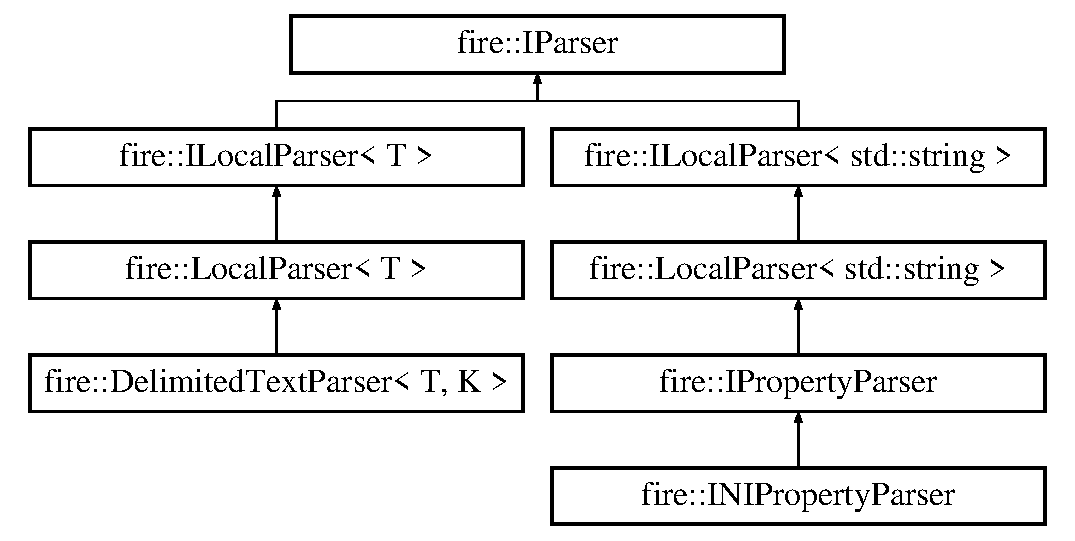
\includegraphics[height=5.000000cm]{a01283}
\end{center}
\end{figure}
\subsection*{Public Member Functions}
\begin{DoxyCompactItemize}
\item 
virtual void \hyperlink{a01283_a0dbeff2b9bd8dbfb2aad7a424eef87d1}{set\+Source} (const std\+::string \&source)=0
\item 
virtual const std\+::string \& \hyperlink{a01283_ab55d2644dfa6d950d1f874e1e02df095}{get\+Source} ()=0
\item 
virtual void \hyperlink{a01283_a7748a633910e9bfc27411d6bd840496b}{set\+Source} (const std\+::istream \&source)=0
\item 
virtual const std\+::istream \& \hyperlink{a01283_ac94c7a288bf669322b93ba171c43f90e}{get\+Source\+Stream} ()=0
\item 
virtual void \hyperlink{a01283_af36ac6eedd8c27d2f418869193d7d03c}{parse} ()=0
\item 
virtual bool \hyperlink{a01283_a616c42c85d781c916e97f0ad8f1e9010}{is\+File} ()=0
\item 
virtual bool \hyperlink{a01283_a97b9e58493b3cadbc63e670b0b0e759f}{is\+Local} ()=0
\item 
virtual bool \hyperlink{a01283_a83d2882a466d694fb0aea3d846bcbed4}{is\+Parallel} ()=0
\end{DoxyCompactItemize}


\subsection{Detailed Description}
This is the base interface for parsers in Fire and it defines the contract that can be expected of all parsers.

This source string is only a reference to the source or some sort of handle that points to it, such as a file or stream name. The exact type of the source -\/ file, stream, socket, etc. -\/ is determined by the implementing class. Check the documentation of implementing classes for the exact way the source string is used.

I\+Parsers should always be used by setting the source and then parsing the source\+:


\begin{DoxyCode}
IParser parser = ...;\textcolor{comment}{// somehow create your parser}
parser.setSource(sourceName);
parser.parser();
\end{DoxyCode}


Subclasses must always be sure that they implement \hyperlink{a01283_af36ac6eedd8c27d2f418869193d7d03c}{parse()} and \hyperlink{a01283_a0dbeff2b9bd8dbfb2aad7a424eef87d1}{set\+Source()}. 

\subsection{Member Function Documentation}
\mbox{\Hypertarget{a01283_ab55d2644dfa6d950d1f874e1e02df095}\label{a01283_ab55d2644dfa6d950d1f874e1e02df095}} 
\index{fire\+::\+I\+Parser@{fire\+::\+I\+Parser}!get\+Source@{get\+Source}}
\index{get\+Source@{get\+Source}!fire\+::\+I\+Parser@{fire\+::\+I\+Parser}}
\subsubsection{\texorpdfstring{get\+Source()}{getSource()}}
{\footnotesize\ttfamily virtual const std\+::string\& fire\+::\+I\+Parser\+::get\+Source (\begin{DoxyParamCaption}{ }\end{DoxyParamCaption})\hspace{0.3cm}{\ttfamily [pure virtual]}}

This operation gets the data source for the parser. \begin{DoxyReturn}{Returns}
the name of the source 
\end{DoxyReturn}


Implemented in \hyperlink{a01291_aedb7fe10911182525a719963b9b56726}{fire\+::\+Local\+Parser$<$ T $>$}, \hyperlink{a01291_aedb7fe10911182525a719963b9b56726}{fire\+::\+Local\+Parser$<$ std\+::string $>$}, and \hyperlink{a01279_ad02c9a530f20a706d7bb2554813e8d3a}{fire\+::\+I\+N\+I\+Property\+Parser}.

\mbox{\Hypertarget{a01283_ac94c7a288bf669322b93ba171c43f90e}\label{a01283_ac94c7a288bf669322b93ba171c43f90e}} 
\index{fire\+::\+I\+Parser@{fire\+::\+I\+Parser}!get\+Source\+Stream@{get\+Source\+Stream}}
\index{get\+Source\+Stream@{get\+Source\+Stream}!fire\+::\+I\+Parser@{fire\+::\+I\+Parser}}
\subsubsection{\texorpdfstring{get\+Source\+Stream()}{getSourceStream()}}
{\footnotesize\ttfamily virtual const std\+::istream\& fire\+::\+I\+Parser\+::get\+Source\+Stream (\begin{DoxyParamCaption}{ }\end{DoxyParamCaption})\hspace{0.3cm}{\ttfamily [pure virtual]}}

This operation gets the data source for the parser as a stream if and only if it was set as such. \begin{DoxyReturn}{Returns}
source the stream of delimited text data 
\end{DoxyReturn}


Implemented in \hyperlink{a01291_a9bf19a3cc9ae8ac0e6e7a0e7f6212cdc}{fire\+::\+Local\+Parser$<$ T $>$}, and \hyperlink{a01291_a9bf19a3cc9ae8ac0e6e7a0e7f6212cdc}{fire\+::\+Local\+Parser$<$ std\+::string $>$}.

\mbox{\Hypertarget{a01283_a616c42c85d781c916e97f0ad8f1e9010}\label{a01283_a616c42c85d781c916e97f0ad8f1e9010}} 
\index{fire\+::\+I\+Parser@{fire\+::\+I\+Parser}!is\+File@{is\+File}}
\index{is\+File@{is\+File}!fire\+::\+I\+Parser@{fire\+::\+I\+Parser}}
\subsubsection{\texorpdfstring{is\+File()}{isFile()}}
{\footnotesize\ttfamily virtual bool fire\+::\+I\+Parser\+::is\+File (\begin{DoxyParamCaption}{ }\end{DoxyParamCaption})\hspace{0.3cm}{\ttfamily [pure virtual]}}

This operation indicates whether or not the parser\textquotesingle{}s source is a file. \begin{DoxyReturn}{Returns}
true if this parser is working with a file, false otherwise. 
\end{DoxyReturn}


Implemented in \hyperlink{a01275_a091d5cf56bf8f407854ef87f460b2958}{fire\+::\+I\+Local\+Parser$<$ T $>$}, and \hyperlink{a01275_a091d5cf56bf8f407854ef87f460b2958}{fire\+::\+I\+Local\+Parser$<$ std\+::string $>$}.

\mbox{\Hypertarget{a01283_a97b9e58493b3cadbc63e670b0b0e759f}\label{a01283_a97b9e58493b3cadbc63e670b0b0e759f}} 
\index{fire\+::\+I\+Parser@{fire\+::\+I\+Parser}!is\+Local@{is\+Local}}
\index{is\+Local@{is\+Local}!fire\+::\+I\+Parser@{fire\+::\+I\+Parser}}
\subsubsection{\texorpdfstring{is\+Local()}{isLocal()}}
{\footnotesize\ttfamily virtual bool fire\+::\+I\+Parser\+::is\+Local (\begin{DoxyParamCaption}{ }\end{DoxyParamCaption})\hspace{0.3cm}{\ttfamily [pure virtual]}}

This operation indicates whether or not the parser is using a local source. \begin{DoxyReturn}{Returns}
true if this parser is working with a local source, false otherwise. 
\end{DoxyReturn}


Implemented in \hyperlink{a01275_a770acae6e216de3a9c7140a12de25d58}{fire\+::\+I\+Local\+Parser$<$ T $>$}, and \hyperlink{a01275_a770acae6e216de3a9c7140a12de25d58}{fire\+::\+I\+Local\+Parser$<$ std\+::string $>$}.

\mbox{\Hypertarget{a01283_a83d2882a466d694fb0aea3d846bcbed4}\label{a01283_a83d2882a466d694fb0aea3d846bcbed4}} 
\index{fire\+::\+I\+Parser@{fire\+::\+I\+Parser}!is\+Parallel@{is\+Parallel}}
\index{is\+Parallel@{is\+Parallel}!fire\+::\+I\+Parser@{fire\+::\+I\+Parser}}
\subsubsection{\texorpdfstring{is\+Parallel()}{isParallel()}}
{\footnotesize\ttfamily virtual bool fire\+::\+I\+Parser\+::is\+Parallel (\begin{DoxyParamCaption}{ }\end{DoxyParamCaption})\hspace{0.3cm}{\ttfamily [pure virtual]}}

This operation indicates whether or not the parser reads in parallel. \begin{DoxyReturn}{Returns}
true if this parser reads in parallel, false otherwise. 
\end{DoxyReturn}


Implemented in \hyperlink{a01275_ad46898c516adcce38acbb4800dc9777b}{fire\+::\+I\+Local\+Parser$<$ T $>$}, and \hyperlink{a01275_ad46898c516adcce38acbb4800dc9777b}{fire\+::\+I\+Local\+Parser$<$ std\+::string $>$}.

\mbox{\Hypertarget{a01283_af36ac6eedd8c27d2f418869193d7d03c}\label{a01283_af36ac6eedd8c27d2f418869193d7d03c}} 
\index{fire\+::\+I\+Parser@{fire\+::\+I\+Parser}!parse@{parse}}
\index{parse@{parse}!fire\+::\+I\+Parser@{fire\+::\+I\+Parser}}
\subsubsection{\texorpdfstring{parse()}{parse()}}
{\footnotesize\ttfamily virtual void fire\+::\+I\+Parser\+::parse (\begin{DoxyParamCaption}{ }\end{DoxyParamCaption})\hspace{0.3cm}{\ttfamily [pure virtual]}}

This operation directs the parser to parse its source. 

Implemented in \hyperlink{a01271_a773fa7ed28cb9d8c384ad94bd81fc93f}{fire\+::\+Delimited\+Text\+Parser$<$ T, K $>$}, \hyperlink{a01271_a686df5548771cae833d5e721442a821a}{fire\+::\+Delimited\+Text\+Parser$<$ T, K $>$}, \hyperlink{a01291_abd8929aea06c2dda40256d2e58236650}{fire\+::\+Local\+Parser$<$ T $>$}, \hyperlink{a01291_abd8929aea06c2dda40256d2e58236650}{fire\+::\+Local\+Parser$<$ std\+::string $>$}, \hyperlink{a01279_a31b6bad01e65ed4bb5f1ba297616c641}{fire\+::\+I\+N\+I\+Property\+Parser}, \hyperlink{a01291_ae904e264fe16708b3e434adea59e1b88}{fire\+::\+Local\+Parser$<$ T $>$}, \hyperlink{a01291_ae904e264fe16708b3e434adea59e1b88}{fire\+::\+Local\+Parser$<$ std\+::string $>$}, \hyperlink{a01291_a34fd9ffb0196c612c75b5288ed5e219b}{fire\+::\+Local\+Parser$<$ T $>$}, and \hyperlink{a01291_a34fd9ffb0196c612c75b5288ed5e219b}{fire\+::\+Local\+Parser$<$ std\+::string $>$}.

\mbox{\Hypertarget{a01283_a0dbeff2b9bd8dbfb2aad7a424eef87d1}\label{a01283_a0dbeff2b9bd8dbfb2aad7a424eef87d1}} 
\index{fire\+::\+I\+Parser@{fire\+::\+I\+Parser}!set\+Source@{set\+Source}}
\index{set\+Source@{set\+Source}!fire\+::\+I\+Parser@{fire\+::\+I\+Parser}}
\subsubsection{\texorpdfstring{set\+Source()}{setSource()}\hspace{0.1cm}{\footnotesize\ttfamily [1/2]}}
{\footnotesize\ttfamily virtual void fire\+::\+I\+Parser\+::set\+Source (\begin{DoxyParamCaption}\item[{const std\+::string \&}]{source }\end{DoxyParamCaption})\hspace{0.3cm}{\ttfamily [pure virtual]}}

This operation sets the data source for the parser. 
\begin{DoxyParams}{Parameters}
{\em source} & the name of the source that the parser should parse. \\
\hline
\end{DoxyParams}


Implemented in \hyperlink{a01291_afcaec6429fdd6e5d53642a32c001ff73}{fire\+::\+Local\+Parser$<$ T $>$}, \hyperlink{a01291_afcaec6429fdd6e5d53642a32c001ff73}{fire\+::\+Local\+Parser$<$ std\+::string $>$}, and \hyperlink{a01279_a06793909bc707a69d0c5772b14bc946d}{fire\+::\+I\+N\+I\+Property\+Parser}.

\mbox{\Hypertarget{a01283_a7748a633910e9bfc27411d6bd840496b}\label{a01283_a7748a633910e9bfc27411d6bd840496b}} 
\index{fire\+::\+I\+Parser@{fire\+::\+I\+Parser}!set\+Source@{set\+Source}}
\index{set\+Source@{set\+Source}!fire\+::\+I\+Parser@{fire\+::\+I\+Parser}}
\subsubsection{\texorpdfstring{set\+Source()}{setSource()}\hspace{0.1cm}{\footnotesize\ttfamily [2/2]}}
{\footnotesize\ttfamily virtual void fire\+::\+I\+Parser\+::set\+Source (\begin{DoxyParamCaption}\item[{const std\+::istream \&}]{source }\end{DoxyParamCaption})\hspace{0.3cm}{\ttfamily [pure virtual]}}

This operation sets the data source for the parser using a stream instead of a string. 
\begin{DoxyParams}{Parameters}
{\em source} & the stream of delimited text data \\
\hline
\end{DoxyParams}


Implemented in \hyperlink{a01291_aed4357541f2ff7d46f8846bd07bb3c42}{fire\+::\+Local\+Parser$<$ T $>$}, and \hyperlink{a01291_aed4357541f2ff7d46f8846bd07bb3c42}{fire\+::\+Local\+Parser$<$ std\+::string $>$}.



The documentation for this class was generated from the following file\+:\begin{DoxyCompactItemize}
\item 
I\+Parser.\+h\end{DoxyCompactItemize}

\hypertarget{a01287}{}\section{fire\+:\+:I\+Property\+Parser Class Reference}
\label{a01287}\index{fire\+::\+I\+Property\+Parser@{fire\+::\+I\+Property\+Parser}}


{\ttfamily \#include $<$I\+Property\+Parser.\+h$>$}

Inheritance diagram for fire\+:\+:I\+Property\+Parser\+:\begin{figure}[H]
\begin{center}
\leavevmode
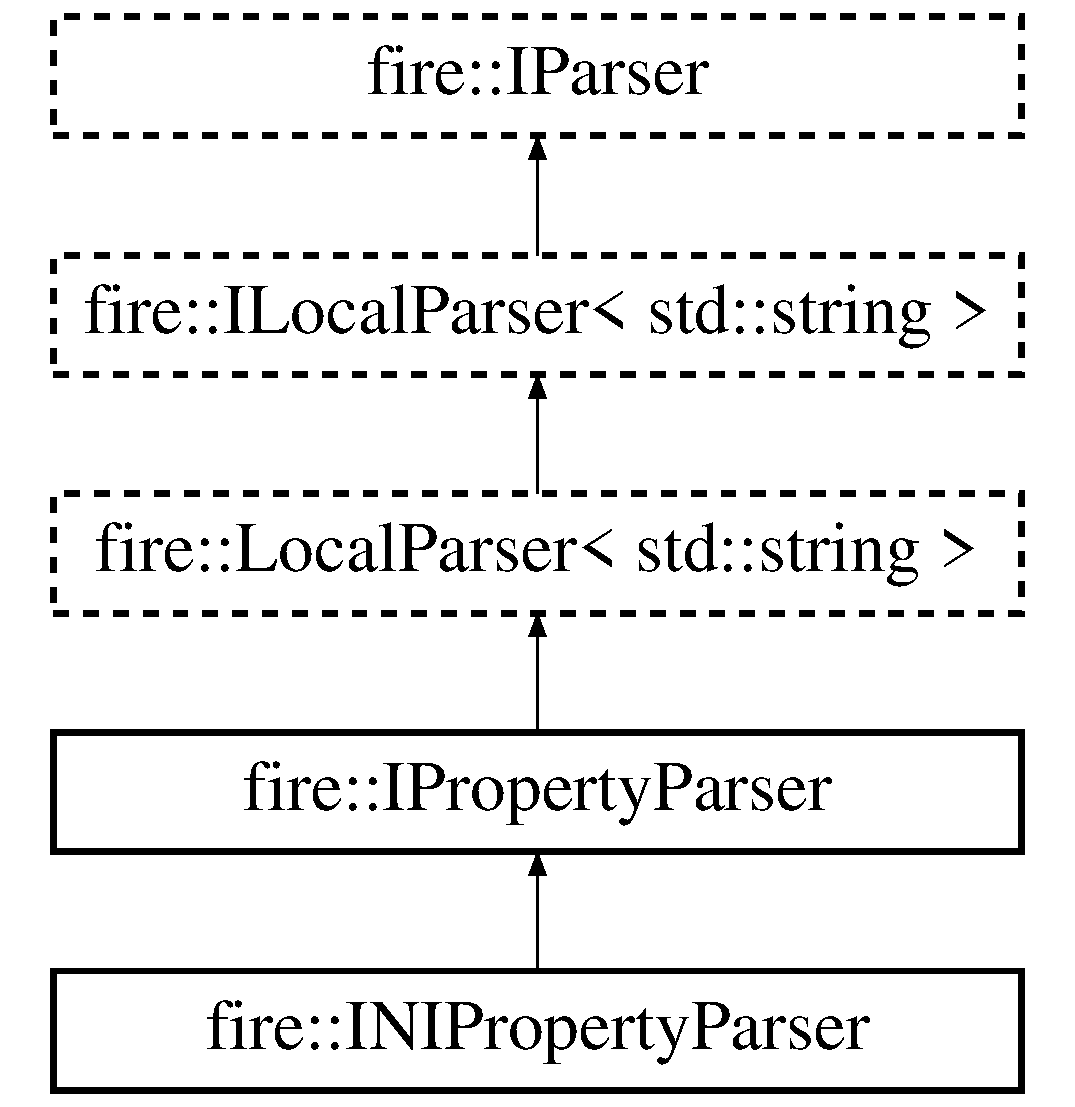
\includegraphics[height=5.000000cm]{a01287}
\end{center}
\end{figure}
\subsection*{Public Member Functions}
\begin{DoxyCompactItemize}
\item 
virtual const std\+::vector$<$ std\+::string $>$ \& \hyperlink{a01287_a34602687f9d1affac7bd842102d4a6aa}{get\+Property\+Block\+Names} ()=0
\item 
virtual const std\+::map$<$ std\+::string, std\+::string $>$ \& \hyperlink{a01287_a34201371cb36dd09e96a66242ececb86}{get\+Property\+Block} (const std\+::string \&name)=0
\end{DoxyCompactItemize}
\subsection*{Additional Inherited Members}


\subsection{Detailed Description}
This is an extension of the parser interface that focuses on parsing a set of properties. Properties are returned in blocks represented by maps.. 

\subsection{Member Function Documentation}
\mbox{\Hypertarget{a01287_a34201371cb36dd09e96a66242ececb86}\label{a01287_a34201371cb36dd09e96a66242ececb86}} 
\index{fire\+::\+I\+Property\+Parser@{fire\+::\+I\+Property\+Parser}!get\+Property\+Block@{get\+Property\+Block}}
\index{get\+Property\+Block@{get\+Property\+Block}!fire\+::\+I\+Property\+Parser@{fire\+::\+I\+Property\+Parser}}
\subsubsection{\texorpdfstring{get\+Property\+Block()}{getPropertyBlock()}}
{\footnotesize\ttfamily virtual const std\+::map$<$std\+::string, std\+::string$>$\& fire\+::\+I\+Property\+Parser\+::get\+Property\+Block (\begin{DoxyParamCaption}\item[{const std\+::string \&}]{name }\end{DoxyParamCaption})\hspace{0.3cm}{\ttfamily [pure virtual]}}

This operation returns the property block with the given name. 
\begin{DoxyParams}{Parameters}
{\em name} & the block name \\
\hline
\end{DoxyParams}
\begin{DoxyReturn}{Returns}
the property block with the given name 
\end{DoxyReturn}


Implemented in \hyperlink{a01279_a3591312590a66659ebd377cdde9ab9ad}{fire\+::\+I\+N\+I\+Property\+Parser}.

\mbox{\Hypertarget{a01287_a34602687f9d1affac7bd842102d4a6aa}\label{a01287_a34602687f9d1affac7bd842102d4a6aa}} 
\index{fire\+::\+I\+Property\+Parser@{fire\+::\+I\+Property\+Parser}!get\+Property\+Block\+Names@{get\+Property\+Block\+Names}}
\index{get\+Property\+Block\+Names@{get\+Property\+Block\+Names}!fire\+::\+I\+Property\+Parser@{fire\+::\+I\+Property\+Parser}}
\subsubsection{\texorpdfstring{get\+Property\+Block\+Names()}{getPropertyBlockNames()}}
{\footnotesize\ttfamily virtual const std\+::vector$<$std\+::string$>$\& fire\+::\+I\+Property\+Parser\+::get\+Property\+Block\+Names (\begin{DoxyParamCaption}{ }\end{DoxyParamCaption})\hspace{0.3cm}{\ttfamily [pure virtual]}}

This operation returns the names of the property blocks parsed from the source. \begin{DoxyReturn}{Returns}
the block names 
\end{DoxyReturn}


Implemented in \hyperlink{a01279_aed0f1f47111794659564dcddb4d25bc6}{fire\+::\+I\+N\+I\+Property\+Parser}.



The documentation for this class was generated from the following file\+:\begin{DoxyCompactItemize}
\item 
I\+Property\+Parser.\+h\end{DoxyCompactItemize}

\hypertarget{a01499}{}\section{xacc\+:\+:IR Class Reference}
\label{a01499}\index{xacc\+::\+IR@{xacc\+::\+IR}}


{\ttfamily \#include $<$I\+R.\+hpp$>$}

Inheritance diagram for xacc\+:\+:IR\+:\begin{figure}[H]
\begin{center}
\leavevmode
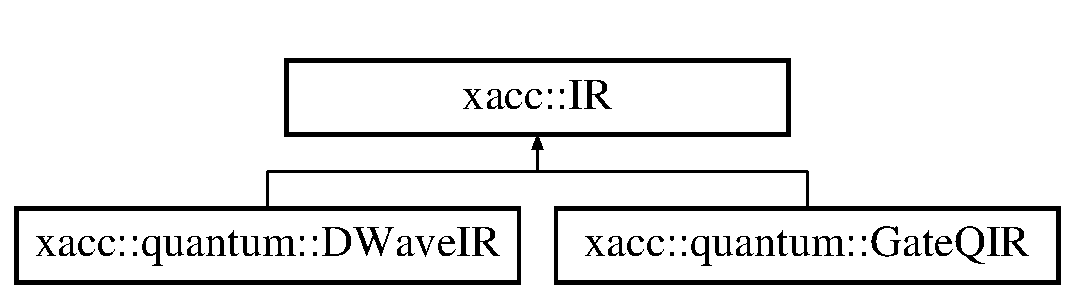
\includegraphics[height=2.000000cm]{a01499}
\end{center}
\end{figure}
\subsection*{Public Member Functions}
\begin{DoxyCompactItemize}
\item 
virtual std\+::string \hyperlink{a01499_a8356cdff1919b88eabeb84fd7450cdb6}{to\+Assembly\+String} (const std\+::string \&kernel\+Name, const std\+::string \&acc\+Buffer\+Var\+Name)=0
\item 
virtual void \hyperlink{a01499_a414b72224d88473ad6190bb88102a3ea}{persist} (std\+::ostream \&out\+Stream)=0
\item 
virtual void \hyperlink{a01499_a444c2e4dc0faac500fb70fa93997e9bc}{load} (std\+::istream \&in\+Stream)=0
\item 
virtual void \hyperlink{a01499_abbbf8e6993c518597de32cd05d49d737}{add\+Kernel} (std\+::shared\+\_\+ptr$<$ \hyperlink{a01475}{Function} $>$ kernel)=0
\item 
virtual bool \hyperlink{a01499_afc9ccf5126f3fed19c2e879133b2f6d8}{kernel\+Exists} (const std\+::string \&name)=0
\item 
virtual std\+::shared\+\_\+ptr$<$ \hyperlink{a01475}{Function} $>$ \hyperlink{a01499_a6f49b4ba4b3a15142b04873284885f0d}{get\+Kernel} (const std\+::string \&name)=0
\item 
virtual std\+::vector$<$ std\+::shared\+\_\+ptr$<$ \hyperlink{a01475}{Function} $>$ $>$ \hyperlink{a01499_a88c50bfc5b279145360ddc0c3a703b9b}{get\+Kernels} ()=0
\item 
virtual \hyperlink{a01499_a09a76d71092254acae07e19fa2f34921}{$\sim$\+IR} ()
\end{DoxyCompactItemize}


\subsection{Detailed Description}
The \hyperlink{a01499}{IR} interface is the base interface for derived accelerator-\/specific intermediate representations. At this level, an intermediate representation can be persisted to an assembly-\/like string, can be read in from file, and can be persisted to file. Since all X\+A\+CC intermediate representations operate on an \hyperlink{a01435}{Accelerator} Buffer, the \hyperlink{a01499}{IR} interface also provides a setter for such a buffer. 

\subsection{Constructor \& Destructor Documentation}
\mbox{\Hypertarget{a01499_a09a76d71092254acae07e19fa2f34921}\label{a01499_a09a76d71092254acae07e19fa2f34921}} 
\index{xacc\+::\+IR@{xacc\+::\+IR}!````~IR@{$\sim$\+IR}}
\index{````~IR@{$\sim$\+IR}!xacc\+::\+IR@{xacc\+::\+IR}}
\subsubsection{\texorpdfstring{$\sim$\+I\+R()}{~IR()}}
{\footnotesize\ttfamily virtual xacc\+::\+I\+R\+::$\sim$\+IR (\begin{DoxyParamCaption}{ }\end{DoxyParamCaption})\hspace{0.3cm}{\ttfamily [inline]}, {\ttfamily [virtual]}}

The destructor 

\subsection{Member Function Documentation}
\mbox{\Hypertarget{a01499_abbbf8e6993c518597de32cd05d49d737}\label{a01499_abbbf8e6993c518597de32cd05d49d737}} 
\index{xacc\+::\+IR@{xacc\+::\+IR}!add\+Kernel@{add\+Kernel}}
\index{add\+Kernel@{add\+Kernel}!xacc\+::\+IR@{xacc\+::\+IR}}
\subsubsection{\texorpdfstring{add\+Kernel()}{addKernel()}}
{\footnotesize\ttfamily virtual void xacc\+::\+I\+R\+::add\+Kernel (\begin{DoxyParamCaption}\item[{std\+::shared\+\_\+ptr$<$ \hyperlink{a01475}{Function} $>$}]{kernel }\end{DoxyParamCaption})\hspace{0.3cm}{\ttfamily [pure virtual]}}

Add a new kernel to this \hyperlink{a01499}{IR} instance.


\begin{DoxyParams}{Parameters}
{\em kernel} & The \hyperlink{a01475}{Function} instance to add as a new kernel \\
\hline
\end{DoxyParams}


Implemented in \hyperlink{a01171_aa6ed2cf2cbcfec8105c327a4fa95346f}{xacc\+::quantum\+::\+Gate\+Q\+IR}, and \hyperlink{a01131_a7e1ddff2771233dc45f60a6b7e15ef63}{xacc\+::quantum\+::\+D\+Wave\+IR}.

\mbox{\Hypertarget{a01499_a6f49b4ba4b3a15142b04873284885f0d}\label{a01499_a6f49b4ba4b3a15142b04873284885f0d}} 
\index{xacc\+::\+IR@{xacc\+::\+IR}!get\+Kernel@{get\+Kernel}}
\index{get\+Kernel@{get\+Kernel}!xacc\+::\+IR@{xacc\+::\+IR}}
\subsubsection{\texorpdfstring{get\+Kernel()}{getKernel()}}
{\footnotesize\ttfamily virtual std\+::shared\+\_\+ptr$<$\hyperlink{a01475}{Function}$>$ xacc\+::\+I\+R\+::get\+Kernel (\begin{DoxyParamCaption}\item[{const std\+::string \&}]{name }\end{DoxyParamCaption})\hspace{0.3cm}{\ttfamily [pure virtual]}}

Return the kernel with the given name.


\begin{DoxyParams}{Parameters}
{\em name} & The name of the kernel to return. \\
\hline
\end{DoxyParams}
\begin{DoxyReturn}{Returns}
kernel The kernel with given name. 
\end{DoxyReturn}


Implemented in \hyperlink{a01171_a194758b6edcc3ae0c7fe8004f9bfe690}{xacc\+::quantum\+::\+Gate\+Q\+IR}, and \hyperlink{a01131_ac4295dfef98c94d7154a4fd39a6e5d1c}{xacc\+::quantum\+::\+D\+Wave\+IR}.

\mbox{\Hypertarget{a01499_a88c50bfc5b279145360ddc0c3a703b9b}\label{a01499_a88c50bfc5b279145360ddc0c3a703b9b}} 
\index{xacc\+::\+IR@{xacc\+::\+IR}!get\+Kernels@{get\+Kernels}}
\index{get\+Kernels@{get\+Kernels}!xacc\+::\+IR@{xacc\+::\+IR}}
\subsubsection{\texorpdfstring{get\+Kernels()}{getKernels()}}
{\footnotesize\ttfamily virtual std\+::vector$<$std\+::shared\+\_\+ptr$<$\hyperlink{a01475}{Function}$>$ $>$ xacc\+::\+I\+R\+::get\+Kernels (\begin{DoxyParamCaption}{ }\end{DoxyParamCaption})\hspace{0.3cm}{\ttfamily [pure virtual]}}

Return all of this \hyperlink{a01499}{IR} instance\textquotesingle{}s kernels.

\begin{DoxyReturn}{Returns}
kernels The kernels this \hyperlink{a01499}{IR} contains. 
\end{DoxyReturn}


Implemented in \hyperlink{a01171_a4ace7ee5ebef84b1f39aaf5ed12c6cc6}{xacc\+::quantum\+::\+Gate\+Q\+IR}, and \hyperlink{a01131_accffbb279cb1f67e0fe79c603fe7a949}{xacc\+::quantum\+::\+D\+Wave\+IR}.

\mbox{\Hypertarget{a01499_afc9ccf5126f3fed19c2e879133b2f6d8}\label{a01499_afc9ccf5126f3fed19c2e879133b2f6d8}} 
\index{xacc\+::\+IR@{xacc\+::\+IR}!kernel\+Exists@{kernel\+Exists}}
\index{kernel\+Exists@{kernel\+Exists}!xacc\+::\+IR@{xacc\+::\+IR}}
\subsubsection{\texorpdfstring{kernel\+Exists()}{kernelExists()}}
{\footnotesize\ttfamily virtual bool xacc\+::\+I\+R\+::kernel\+Exists (\begin{DoxyParamCaption}\item[{const std\+::string \&}]{name }\end{DoxyParamCaption})\hspace{0.3cm}{\ttfamily [pure virtual]}}

Return true if the kernel with given name exists in this \hyperlink{a01499}{IR}.


\begin{DoxyParams}{Parameters}
{\em name} & The name of the kernel to return. \\
\hline
\end{DoxyParams}
\begin{DoxyReturn}{Returns}
exists True if kernel exists. 
\end{DoxyReturn}


Implemented in \hyperlink{a01171_a692f95099caa7c024110a3f035941dca}{xacc\+::quantum\+::\+Gate\+Q\+IR}, and \hyperlink{a01131_ace9b8c6f4f29e32c8482fec4eacb637a}{xacc\+::quantum\+::\+D\+Wave\+IR}.

\mbox{\Hypertarget{a01499_a444c2e4dc0faac500fb70fa93997e9bc}\label{a01499_a444c2e4dc0faac500fb70fa93997e9bc}} 
\index{xacc\+::\+IR@{xacc\+::\+IR}!load@{load}}
\index{load@{load}!xacc\+::\+IR@{xacc\+::\+IR}}
\subsubsection{\texorpdfstring{load()}{load()}}
{\footnotesize\ttfamily virtual void xacc\+::\+I\+R\+::load (\begin{DoxyParamCaption}\item[{std\+::istream \&}]{in\+Stream }\end{DoxyParamCaption})\hspace{0.3cm}{\ttfamily [pure virtual]}}

Create this \hyperlink{a01499}{IR} instance from the given input stream.


\begin{DoxyParams}{Parameters}
{\em in\+Stream} & The input stream to read from. \\
\hline
\end{DoxyParams}


Implemented in \hyperlink{a01171_a07f26eeb362ac480d20da6cdc8c8fb39}{xacc\+::quantum\+::\+Gate\+Q\+IR}, and \hyperlink{a01131_a94d814172ec30c7ed32e6ab52bc2a41a}{xacc\+::quantum\+::\+D\+Wave\+IR}.

\mbox{\Hypertarget{a01499_a414b72224d88473ad6190bb88102a3ea}\label{a01499_a414b72224d88473ad6190bb88102a3ea}} 
\index{xacc\+::\+IR@{xacc\+::\+IR}!persist@{persist}}
\index{persist@{persist}!xacc\+::\+IR@{xacc\+::\+IR}}
\subsubsection{\texorpdfstring{persist()}{persist()}}
{\footnotesize\ttfamily virtual void xacc\+::\+I\+R\+::persist (\begin{DoxyParamCaption}\item[{std\+::ostream \&}]{out\+Stream }\end{DoxyParamCaption})\hspace{0.3cm}{\ttfamily [pure virtual]}}

Persist this \hyperlink{a01499}{IR} instance to the given output stream.


\begin{DoxyParams}{Parameters}
{\em out\+Stream} & The output stream to persist to. \\
\hline
\end{DoxyParams}


Implemented in \hyperlink{a01171_a40e1d07e4dfd3794ef53fca3cdbdca61}{xacc\+::quantum\+::\+Gate\+Q\+IR}, and \hyperlink{a01131_adac268c6fa2234902efeb9b3c07c0ac2}{xacc\+::quantum\+::\+D\+Wave\+IR}.

\mbox{\Hypertarget{a01499_a8356cdff1919b88eabeb84fd7450cdb6}\label{a01499_a8356cdff1919b88eabeb84fd7450cdb6}} 
\index{xacc\+::\+IR@{xacc\+::\+IR}!to\+Assembly\+String@{to\+Assembly\+String}}
\index{to\+Assembly\+String@{to\+Assembly\+String}!xacc\+::\+IR@{xacc\+::\+IR}}
\subsubsection{\texorpdfstring{to\+Assembly\+String()}{toAssemblyString()}}
{\footnotesize\ttfamily virtual std\+::string xacc\+::\+I\+R\+::to\+Assembly\+String (\begin{DoxyParamCaption}\item[{const std\+::string \&}]{kernel\+Name,  }\item[{const std\+::string \&}]{acc\+Buffer\+Var\+Name }\end{DoxyParamCaption})\hspace{0.3cm}{\ttfamily [pure virtual]}}

Return a assembly-\/like string representation of this intermediate representation


\begin{DoxyParams}{Parameters}
{\em kernel\+Name} & The name of hte kernel to persist to string \\
\hline
{\em acc\+Buffer\+Var\+Name} & The name of the \hyperlink{a01447}{Accelerator\+Buffer} \\
\hline
\end{DoxyParams}
\begin{DoxyReturn}{Returns}

\end{DoxyReturn}


Implemented in \hyperlink{a01171_a7153f7e9f516d43af3d5d4f95d60bd86}{xacc\+::quantum\+::\+Gate\+Q\+IR}, and \hyperlink{a01131_ac19ad098d5bbfe769809c10e26ebebc6}{xacc\+::quantum\+::\+D\+Wave\+IR}.



The documentation for this class was generated from the following file\+:\begin{DoxyCompactItemize}
\item 
I\+R.\+hpp\end{DoxyCompactItemize}

\hypertarget{a01503}{}\section{xacc\+:\+:I\+R\+Transformation Class Reference}
\label{a01503}\index{xacc\+::\+I\+R\+Transformation@{xacc\+::\+I\+R\+Transformation}}
\subsection*{Public Member Functions}
\begin{DoxyCompactItemize}
\item 
\mbox{\Hypertarget{a01503_accc69cba97f39aa3e51f81fec3ccf258}\label{a01503_accc69cba97f39aa3e51f81fec3ccf258}} 
virtual void {\bfseries transform} (\hyperlink{a01499}{IR} \&ir)=0
\end{DoxyCompactItemize}


The documentation for this class was generated from the following file\+:\begin{DoxyCompactItemize}
\item 
I\+R\+Transformation.\+hpp\end{DoxyCompactItemize}

\hypertarget{a01515}{}\section{xacc\+:\+:is\+\_\+valid\+\_\+vertex$<$ T, typename $>$ Struct Template Reference}
\label{a01515}\index{xacc\+::is\+\_\+valid\+\_\+vertex$<$ T, typename $>$@{xacc\+::is\+\_\+valid\+\_\+vertex$<$ T, typename $>$}}


{\ttfamily \#include $<$Graph.\+hpp$>$}

Inheritance diagram for xacc\+:\+:is\+\_\+valid\+\_\+vertex$<$ T, typename $>$\+:\begin{figure}[H]
\begin{center}
\leavevmode
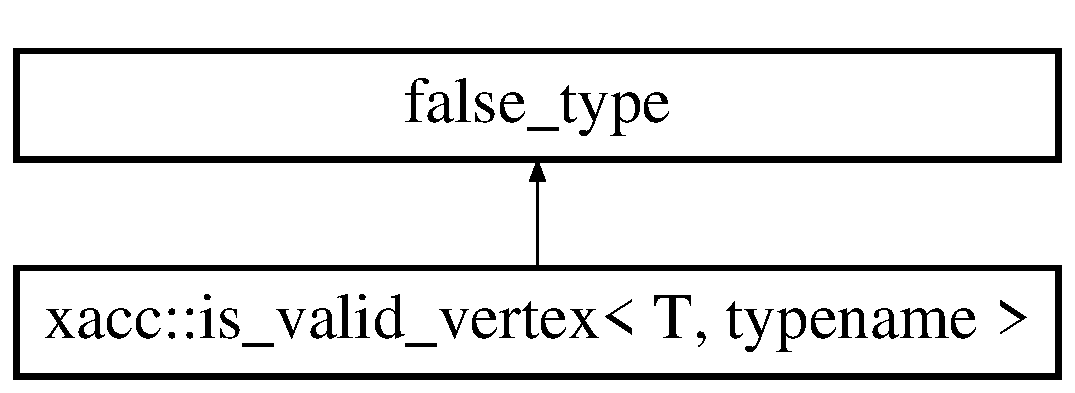
\includegraphics[height=2.000000cm]{a01515}
\end{center}
\end{figure}


\subsection{Detailed Description}
\subsubsection*{template$<$typename T, typename = void$>$\newline
struct xacc\+::is\+\_\+valid\+\_\+vertex$<$ T, typename $>$}

Utility structs to help determine if we have been given valid Vertices. 

The documentation for this struct was generated from the following file\+:\begin{DoxyCompactItemize}
\item 
Graph.\+hpp\end{DoxyCompactItemize}

\hypertarget{a01519}{}\section{xacc\+:\+:is\+\_\+valid\+\_\+vertex$<$ T, decltype(std\+:\+:declval$<$ T $>$().properties, void())$>$ Struct Template Reference}
\label{a01519}\index{xacc\+::is\+\_\+valid\+\_\+vertex$<$ T, decltype(std\+::declval$<$ T $>$().\+properties, void())$>$@{xacc\+::is\+\_\+valid\+\_\+vertex$<$ T, decltype(std\+::declval$<$ T $>$().\+properties, void())$>$}}
Inheritance diagram for xacc\+:\+:is\+\_\+valid\+\_\+vertex$<$ T, decltype(std\+:\+:declval$<$ T $>$().properties, void())$>$\+:\begin{figure}[H]
\begin{center}
\leavevmode
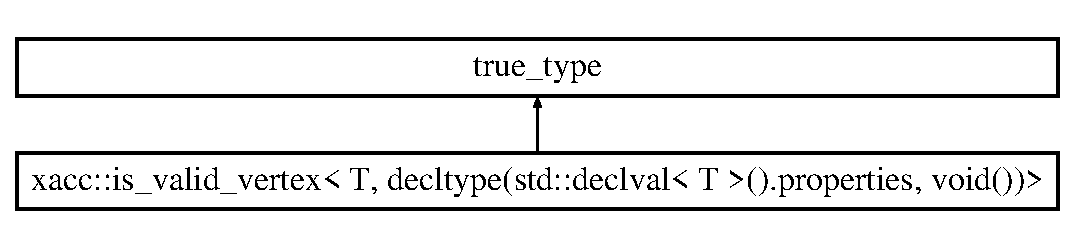
\includegraphics[height=2.000000cm]{a01519}
\end{center}
\end{figure}


The documentation for this struct was generated from the following file\+:\begin{DoxyCompactItemize}
\item 
Graph.\+hpp\end{DoxyCompactItemize}

\hypertarget{a01263}{}\section{fire\+:\+:I\+Stepper Class Reference}
\label{a01263}\index{fire\+::\+I\+Stepper@{fire\+::\+I\+Stepper}}


{\ttfamily \#include $<$I\+Stepper.\+h$>$}

Inheritance diagram for fire\+:\+:I\+Stepper\+:\begin{figure}[H]
\begin{center}
\leavevmode
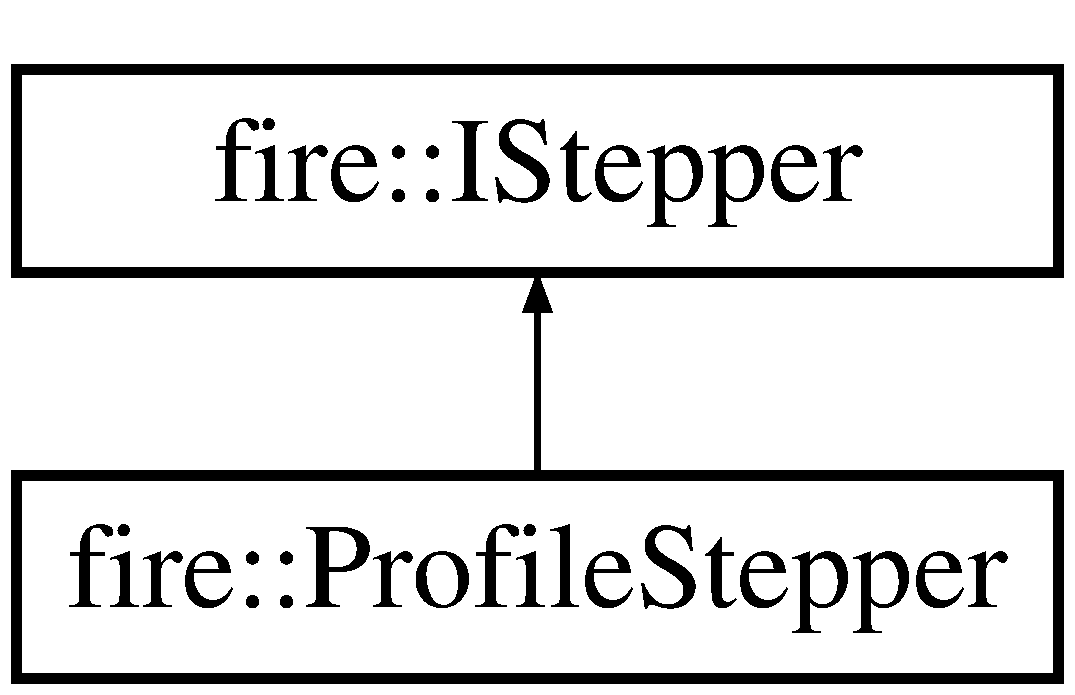
\includegraphics[height=2.000000cm]{a01263}
\end{center}
\end{figure}
\subsection*{Public Member Functions}
\begin{DoxyCompactItemize}
\item 
virtual double \hyperlink{a01263_a7f709d1462a2a3b8bd8214cc681ca26e}{get\+Step} ()=0
\item 
virtual double \hyperlink{a01263_a43027c0c268afcd59db8815c2e2c41ea}{get\+Step\+Size\+At\+Stage} (int i)=0
\item 
virtual void \hyperlink{a01263_a44dfccb90ee5ef6e080b54113c215458}{update\+Step} ()=0
\item 
virtual void \hyperlink{a01263_a3a5099cd0f3c874e56c33cb8f13b8f3b}{set\+Initial\+Step} (double initial\+Step)=0
\item 
virtual double \hyperlink{a01263_a49df3a2ac05cebaf2baf387b66d19272}{get\+Initial\+Step} ()=0
\item 
virtual void \hyperlink{a01263_add76974a7b6fbbc93916270a376c461e}{set\+Final\+Step} (double final\+Step)=0
\item 
virtual double \hyperlink{a01263_ab234d9f032e02668aededf1c22e8c0a9}{get\+Final\+Step} ()=0
\item 
virtual void \hyperlink{a01263_a69c262f248511efcd271be1724a41ad9}{set\+Initial\+Stepsize} (double step\+Size)=0
\item 
virtual double \hyperlink{a01263_afb777e62386b25e5a38d59af54972690}{get\+Initial\+Stepsize} ()=0
\item 
virtual \hyperlink{a01263_ac8ec460d35512e2e039396d5192eb57e}{$\sim$\+I\+Stepper} ()
\end{DoxyCompactItemize}


\subsection{Detailed Description}
This is an interface for managing discrete steps as required by Initial Value Problem Integrators. \hyperlink{a01263}{I\+Stepper} implementations track both the step and the stepsize. In the case of time-\/dependent initial value problems, implementations would be called \char`\"{}time steppers\char`\"{} and would be responsible for computing both the present time (the step) and the step between the present size and the next (the step size). In purely spatial or otherwise on-\/temporal problems, the step represents the current value of the independent variable and the step size represents the distance between the present and next steps.

This interface is designed for single-\/ and multi-\/stage solvers, such as Runge-\/\+Kutta solvers. 

\subsection{Constructor \& Destructor Documentation}
\mbox{\Hypertarget{a01263_ac8ec460d35512e2e039396d5192eb57e}\label{a01263_ac8ec460d35512e2e039396d5192eb57e}} 
\index{fire\+::\+I\+Stepper@{fire\+::\+I\+Stepper}!````~I\+Stepper@{$\sim$\+I\+Stepper}}
\index{````~I\+Stepper@{$\sim$\+I\+Stepper}!fire\+::\+I\+Stepper@{fire\+::\+I\+Stepper}}
\subsubsection{\texorpdfstring{$\sim$\+I\+Stepper()}{~IStepper()}}
{\footnotesize\ttfamily virtual fire\+::\+I\+Stepper\+::$\sim$\+I\+Stepper (\begin{DoxyParamCaption}{ }\end{DoxyParamCaption})\hspace{0.3cm}{\ttfamily [inline]}, {\ttfamily [virtual]}}

Virtual Destructor 

\subsection{Member Function Documentation}
\mbox{\Hypertarget{a01263_ab234d9f032e02668aededf1c22e8c0a9}\label{a01263_ab234d9f032e02668aededf1c22e8c0a9}} 
\index{fire\+::\+I\+Stepper@{fire\+::\+I\+Stepper}!get\+Final\+Step@{get\+Final\+Step}}
\index{get\+Final\+Step@{get\+Final\+Step}!fire\+::\+I\+Stepper@{fire\+::\+I\+Stepper}}
\subsubsection{\texorpdfstring{get\+Final\+Step()}{getFinalStep()}}
{\footnotesize\ttfamily virtual double fire\+::\+I\+Stepper\+::get\+Final\+Step (\begin{DoxyParamCaption}{ }\end{DoxyParamCaption})\hspace{0.3cm}{\ttfamily [pure virtual]}}

This operation returns the final step for the stepper. \begin{DoxyReturn}{Returns}
the final step 
\end{DoxyReturn}


Implemented in \hyperlink{a01267_ae6f257aca7b3bb62a851169a01bcaacf}{fire\+::\+Profile\+Stepper}.

\mbox{\Hypertarget{a01263_a49df3a2ac05cebaf2baf387b66d19272}\label{a01263_a49df3a2ac05cebaf2baf387b66d19272}} 
\index{fire\+::\+I\+Stepper@{fire\+::\+I\+Stepper}!get\+Initial\+Step@{get\+Initial\+Step}}
\index{get\+Initial\+Step@{get\+Initial\+Step}!fire\+::\+I\+Stepper@{fire\+::\+I\+Stepper}}
\subsubsection{\texorpdfstring{get\+Initial\+Step()}{getInitialStep()}}
{\footnotesize\ttfamily virtual double fire\+::\+I\+Stepper\+::get\+Initial\+Step (\begin{DoxyParamCaption}{ }\end{DoxyParamCaption})\hspace{0.3cm}{\ttfamily [pure virtual]}}

This operation returns the initial step for the stepper. \begin{DoxyReturn}{Returns}
the initial step 
\end{DoxyReturn}


Implemented in \hyperlink{a01267_af24660fa4bd027f877d5c1bdeb286cf5}{fire\+::\+Profile\+Stepper}.

\mbox{\Hypertarget{a01263_afb777e62386b25e5a38d59af54972690}\label{a01263_afb777e62386b25e5a38d59af54972690}} 
\index{fire\+::\+I\+Stepper@{fire\+::\+I\+Stepper}!get\+Initial\+Stepsize@{get\+Initial\+Stepsize}}
\index{get\+Initial\+Stepsize@{get\+Initial\+Stepsize}!fire\+::\+I\+Stepper@{fire\+::\+I\+Stepper}}
\subsubsection{\texorpdfstring{get\+Initial\+Stepsize()}{getInitialStepsize()}}
{\footnotesize\ttfamily virtual double fire\+::\+I\+Stepper\+::get\+Initial\+Stepsize (\begin{DoxyParamCaption}{ }\end{DoxyParamCaption})\hspace{0.3cm}{\ttfamily [pure virtual]}}

This operation gets the initial step size for the stepper \begin{DoxyReturn}{Returns}
the initial step size 
\end{DoxyReturn}


Implemented in \hyperlink{a01267_a86e7035366907a08a36722655746271e}{fire\+::\+Profile\+Stepper}.

\mbox{\Hypertarget{a01263_a7f709d1462a2a3b8bd8214cc681ca26e}\label{a01263_a7f709d1462a2a3b8bd8214cc681ca26e}} 
\index{fire\+::\+I\+Stepper@{fire\+::\+I\+Stepper}!get\+Step@{get\+Step}}
\index{get\+Step@{get\+Step}!fire\+::\+I\+Stepper@{fire\+::\+I\+Stepper}}
\subsubsection{\texorpdfstring{get\+Step()}{getStep()}}
{\footnotesize\ttfamily virtual double fire\+::\+I\+Stepper\+::get\+Step (\begin{DoxyParamCaption}{ }\end{DoxyParamCaption})\hspace{0.3cm}{\ttfamily [pure virtual]}}

This operation returns the step value for the current step. \begin{DoxyReturn}{Returns}
the step value 
\end{DoxyReturn}


Implemented in \hyperlink{a01267_a9096ad65a3fcf63678b600cbe0c33961}{fire\+::\+Profile\+Stepper}.

\mbox{\Hypertarget{a01263_a43027c0c268afcd59db8815c2e2c41ea}\label{a01263_a43027c0c268afcd59db8815c2e2c41ea}} 
\index{fire\+::\+I\+Stepper@{fire\+::\+I\+Stepper}!get\+Step\+Size\+At\+Stage@{get\+Step\+Size\+At\+Stage}}
\index{get\+Step\+Size\+At\+Stage@{get\+Step\+Size\+At\+Stage}!fire\+::\+I\+Stepper@{fire\+::\+I\+Stepper}}
\subsubsection{\texorpdfstring{get\+Step\+Size\+At\+Stage()}{getStepSizeAtStage()}}
{\footnotesize\ttfamily virtual double fire\+::\+I\+Stepper\+::get\+Step\+Size\+At\+Stage (\begin{DoxyParamCaption}\item[{int}]{i }\end{DoxyParamCaption})\hspace{0.3cm}{\ttfamily [pure virtual]}}

This operation returns the step size for the given stage. 
\begin{DoxyParams}{Parameters}
{\em the} & stage of the solver for which the stepsize should be computed \\
\hline
\end{DoxyParams}
\begin{DoxyReturn}{Returns}
the step size 
\end{DoxyReturn}


Implemented in \hyperlink{a01267_adaa1a23c068977ecc6809dd8eecab49d}{fire\+::\+Profile\+Stepper}.

\mbox{\Hypertarget{a01263_add76974a7b6fbbc93916270a376c461e}\label{a01263_add76974a7b6fbbc93916270a376c461e}} 
\index{fire\+::\+I\+Stepper@{fire\+::\+I\+Stepper}!set\+Final\+Step@{set\+Final\+Step}}
\index{set\+Final\+Step@{set\+Final\+Step}!fire\+::\+I\+Stepper@{fire\+::\+I\+Stepper}}
\subsubsection{\texorpdfstring{set\+Final\+Step()}{setFinalStep()}}
{\footnotesize\ttfamily virtual void fire\+::\+I\+Stepper\+::set\+Final\+Step (\begin{DoxyParamCaption}\item[{double}]{final\+Step }\end{DoxyParamCaption})\hspace{0.3cm}{\ttfamily [pure virtual]}}

This operation sets the final step for the stepper. 
\begin{DoxyParams}{Parameters}
{\em final\+Step} & the final step \\
\hline
\end{DoxyParams}


Implemented in \hyperlink{a01267_af8203296b4f3bef53bafab7cb654cc97}{fire\+::\+Profile\+Stepper}.

\mbox{\Hypertarget{a01263_a3a5099cd0f3c874e56c33cb8f13b8f3b}\label{a01263_a3a5099cd0f3c874e56c33cb8f13b8f3b}} 
\index{fire\+::\+I\+Stepper@{fire\+::\+I\+Stepper}!set\+Initial\+Step@{set\+Initial\+Step}}
\index{set\+Initial\+Step@{set\+Initial\+Step}!fire\+::\+I\+Stepper@{fire\+::\+I\+Stepper}}
\subsubsection{\texorpdfstring{set\+Initial\+Step()}{setInitialStep()}}
{\footnotesize\ttfamily virtual void fire\+::\+I\+Stepper\+::set\+Initial\+Step (\begin{DoxyParamCaption}\item[{double}]{initial\+Step }\end{DoxyParamCaption})\hspace{0.3cm}{\ttfamily [pure virtual]}}

This operation sets the initial step for the stepper. 
\begin{DoxyParams}{Parameters}
{\em initial\+Step} & the initial step \\
\hline
\end{DoxyParams}


Implemented in \hyperlink{a01267_adf2f78648d9539282225117c0fd243af}{fire\+::\+Profile\+Stepper}.

\mbox{\Hypertarget{a01263_a69c262f248511efcd271be1724a41ad9}\label{a01263_a69c262f248511efcd271be1724a41ad9}} 
\index{fire\+::\+I\+Stepper@{fire\+::\+I\+Stepper}!set\+Initial\+Stepsize@{set\+Initial\+Stepsize}}
\index{set\+Initial\+Stepsize@{set\+Initial\+Stepsize}!fire\+::\+I\+Stepper@{fire\+::\+I\+Stepper}}
\subsubsection{\texorpdfstring{set\+Initial\+Stepsize()}{setInitialStepsize()}}
{\footnotesize\ttfamily virtual void fire\+::\+I\+Stepper\+::set\+Initial\+Stepsize (\begin{DoxyParamCaption}\item[{double}]{step\+Size }\end{DoxyParamCaption})\hspace{0.3cm}{\ttfamily [pure virtual]}}

This operation sets the initial step size for the stepper 
\begin{DoxyParams}{Parameters}
{\em the} & initial step size \\
\hline
\end{DoxyParams}


Implemented in \hyperlink{a01267_a55c44fd97d8b6a474243ad0da48b039d}{fire\+::\+Profile\+Stepper}.

\mbox{\Hypertarget{a01263_a44dfccb90ee5ef6e080b54113c215458}\label{a01263_a44dfccb90ee5ef6e080b54113c215458}} 
\index{fire\+::\+I\+Stepper@{fire\+::\+I\+Stepper}!update\+Step@{update\+Step}}
\index{update\+Step@{update\+Step}!fire\+::\+I\+Stepper@{fire\+::\+I\+Stepper}}
\subsubsection{\texorpdfstring{update\+Step()}{updateStep()}}
{\footnotesize\ttfamily virtual void fire\+::\+I\+Stepper\+::update\+Step (\begin{DoxyParamCaption}{ }\end{DoxyParamCaption})\hspace{0.3cm}{\ttfamily [pure virtual]}}

This operation replaces the current step and stepsize with the next step and stepsize values. 

Implemented in \hyperlink{a01267_a2c13fd4da5550f1e58df2b54bbfe4c2c}{fire\+::\+Profile\+Stepper}.



The documentation for this class was generated from the following file\+:\begin{DoxyCompactItemize}
\item 
I\+Stepper.\+h\end{DoxyCompactItemize}

\hypertarget{a01235}{}\section{xacc\+:\+:runtime\+\_\+get\+\_\+func\+\_\+table$<$ Tuple, Indices $>$ Struct Template Reference}
\label{a01235}\index{xacc\+::runtime\+\_\+get\+\_\+func\+\_\+table$<$ Tuple, Indices $>$@{xacc\+::runtime\+\_\+get\+\_\+func\+\_\+table$<$ Tuple, Indices $>$}}


The documentation for this struct was generated from the following file\+:\begin{DoxyCompactItemize}
\item 
Utils.\+hpp\end{DoxyCompactItemize}

\hypertarget{a01135}{}\section{xacc\+:\+:Instruction\+Iterator Class Reference}
\label{a01135}\index{xacc\+::\+Instruction\+Iterator@{xacc\+::\+Instruction\+Iterator}}


{\ttfamily \#include $<$Instruction\+Iterator.\+hpp$>$}

\subsection*{Public Member Functions}
\begin{DoxyCompactItemize}
\item 
\hyperlink{a01135_af61abf612341ab1454a1c43239b2da16}{Instruction\+Iterator} (std\+::shared\+\_\+ptr$<$ \hyperlink{a01131}{Instruction} $>$ r)
\item 
bool \hyperlink{a01135_a7fa6c8cff43e7b224211d4f7954a4152}{has\+Next} ()
\item 
std\+::shared\+\_\+ptr$<$ \hyperlink{a01131}{Instruction} $>$ \hyperlink{a01135_a0a2e2b1543650760a869460ebcd4382b}{next} ()
\end{DoxyCompactItemize}
\subsection*{Protected Attributes}
\begin{DoxyCompactItemize}
\item 
std\+::shared\+\_\+ptr$<$ \hyperlink{a01131}{Instruction} $>$ \hyperlink{a01135_a9d7aee1cb9058dd4a29c8fc71eeda57d}{root}
\item 
std\+::stack$<$ std\+::shared\+\_\+ptr$<$ \hyperlink{a01131}{Instruction} $>$ $>$ \hyperlink{a01135_a7af48509e563e8865131692c3b71edf0}{inst\+Stack}
\end{DoxyCompactItemize}


\subsection{Detailed Description}
The \hyperlink{a01135}{Instruction\+Iterator} provides a mechanism for a pre-\/order traversal of an \hyperlink{a01131}{Instruction} tree. 

\subsection{Constructor \& Destructor Documentation}
\mbox{\Hypertarget{a01135_af61abf612341ab1454a1c43239b2da16}\label{a01135_af61abf612341ab1454a1c43239b2da16}} 
\index{xacc\+::\+Instruction\+Iterator@{xacc\+::\+Instruction\+Iterator}!Instruction\+Iterator@{Instruction\+Iterator}}
\index{Instruction\+Iterator@{Instruction\+Iterator}!xacc\+::\+Instruction\+Iterator@{xacc\+::\+Instruction\+Iterator}}
\subsubsection{\texorpdfstring{Instruction\+Iterator()}{InstructionIterator()}}
{\footnotesize\ttfamily xacc\+::\+Instruction\+Iterator\+::\+Instruction\+Iterator (\begin{DoxyParamCaption}\item[{std\+::shared\+\_\+ptr$<$ \hyperlink{a01131}{Instruction} $>$}]{r }\end{DoxyParamCaption})\hspace{0.3cm}{\ttfamily [inline]}}

The constructor, takes the root of the tree as input.


\begin{DoxyParams}{Parameters}
{\em r} & \\
\hline
\end{DoxyParams}


\subsection{Member Function Documentation}
\mbox{\Hypertarget{a01135_a7fa6c8cff43e7b224211d4f7954a4152}\label{a01135_a7fa6c8cff43e7b224211d4f7954a4152}} 
\index{xacc\+::\+Instruction\+Iterator@{xacc\+::\+Instruction\+Iterator}!has\+Next@{has\+Next}}
\index{has\+Next@{has\+Next}!xacc\+::\+Instruction\+Iterator@{xacc\+::\+Instruction\+Iterator}}
\subsubsection{\texorpdfstring{has\+Next()}{hasNext()}}
{\footnotesize\ttfamily bool xacc\+::\+Instruction\+Iterator\+::has\+Next (\begin{DoxyParamCaption}{ }\end{DoxyParamCaption})\hspace{0.3cm}{\ttfamily [inline]}}

Return true if there are still instructions left to traverse. \begin{DoxyReturn}{Returns}

\end{DoxyReturn}
\mbox{\Hypertarget{a01135_a0a2e2b1543650760a869460ebcd4382b}\label{a01135_a0a2e2b1543650760a869460ebcd4382b}} 
\index{xacc\+::\+Instruction\+Iterator@{xacc\+::\+Instruction\+Iterator}!next@{next}}
\index{next@{next}!xacc\+::\+Instruction\+Iterator@{xacc\+::\+Instruction\+Iterator}}
\subsubsection{\texorpdfstring{next()}{next()}}
{\footnotesize\ttfamily std\+::shared\+\_\+ptr$<$\hyperlink{a01131}{Instruction}$>$ xacc\+::\+Instruction\+Iterator\+::next (\begin{DoxyParamCaption}{ }\end{DoxyParamCaption})\hspace{0.3cm}{\ttfamily [inline]}}

Return the next \hyperlink{a01131}{Instruction} in the tree. \begin{DoxyReturn}{Returns}

\end{DoxyReturn}


\subsection{Member Data Documentation}
\mbox{\Hypertarget{a01135_a7af48509e563e8865131692c3b71edf0}\label{a01135_a7af48509e563e8865131692c3b71edf0}} 
\index{xacc\+::\+Instruction\+Iterator@{xacc\+::\+Instruction\+Iterator}!inst\+Stack@{inst\+Stack}}
\index{inst\+Stack@{inst\+Stack}!xacc\+::\+Instruction\+Iterator@{xacc\+::\+Instruction\+Iterator}}
\subsubsection{\texorpdfstring{inst\+Stack}{instStack}}
{\footnotesize\ttfamily std\+::stack$<$std\+::shared\+\_\+ptr$<$\hyperlink{a01131}{Instruction}$>$ $>$ xacc\+::\+Instruction\+Iterator\+::inst\+Stack\hspace{0.3cm}{\ttfamily [protected]}}

A stack used to implement the tree traversal \mbox{\Hypertarget{a01135_a9d7aee1cb9058dd4a29c8fc71eeda57d}\label{a01135_a9d7aee1cb9058dd4a29c8fc71eeda57d}} 
\index{xacc\+::\+Instruction\+Iterator@{xacc\+::\+Instruction\+Iterator}!root@{root}}
\index{root@{root}!xacc\+::\+Instruction\+Iterator@{xacc\+::\+Instruction\+Iterator}}
\subsubsection{\texorpdfstring{root}{root}}
{\footnotesize\ttfamily std\+::shared\+\_\+ptr$<$\hyperlink{a01131}{Instruction}$>$ xacc\+::\+Instruction\+Iterator\+::root\hspace{0.3cm}{\ttfamily [protected]}}

The root of the tree, a function 

The documentation for this class was generated from the following file\+:\begin{DoxyCompactItemize}
\item 
Instruction\+Iterator.\+hpp\end{DoxyCompactItemize}

\hypertarget{a01391}{}\section{C\+Simple\+Ini\+Templ$<$ S\+I\+\_\+\+C\+H\+AR, S\+I\+\_\+\+S\+T\+R\+L\+E\+SS, S\+I\+\_\+\+C\+O\+N\+V\+E\+R\+T\+ER $>$\+:\+:Entry\+:\+:Key\+Order Struct Reference}
\label{a01391}\index{C\+Simple\+Ini\+Templ$<$ S\+I\+\_\+\+C\+H\+A\+R, S\+I\+\_\+\+S\+T\+R\+L\+E\+S\+S, S\+I\+\_\+\+C\+O\+N\+V\+E\+R\+T\+E\+R $>$\+::\+Entry\+::\+Key\+Order@{C\+Simple\+Ini\+Templ$<$ S\+I\+\_\+\+C\+H\+A\+R, S\+I\+\_\+\+S\+T\+R\+L\+E\+S\+S, S\+I\+\_\+\+C\+O\+N\+V\+E\+R\+T\+E\+R $>$\+::\+Entry\+::\+Key\+Order}}


{\ttfamily \#include $<$Simple\+Ini.\+h$>$}

Inheritance diagram for C\+Simple\+Ini\+Templ$<$ S\+I\+\_\+\+C\+H\+AR, S\+I\+\_\+\+S\+T\+R\+L\+E\+SS, S\+I\+\_\+\+C\+O\+N\+V\+E\+R\+T\+ER $>$\+:\+:Entry\+:\+:Key\+Order\+:\begin{figure}[H]
\begin{center}
\leavevmode
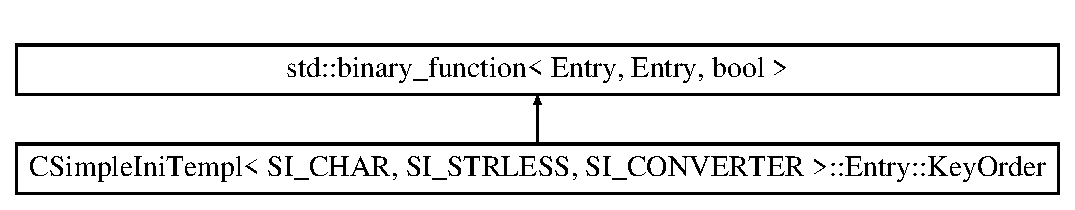
\includegraphics[height=2.000000cm]{a01391}
\end{center}
\end{figure}
\subsection*{Public Member Functions}
\begin{DoxyCompactItemize}
\item 
\mbox{\Hypertarget{a01391_a402ee4ace1311daeaa0eae6c4c83bf87}\label{a01391_a402ee4ace1311daeaa0eae6c4c83bf87}} 
bool {\bfseries operator()} (const \hyperlink{a01387}{Entry} \&lhs, const \hyperlink{a01387}{Entry} \&rhs) const
\end{DoxyCompactItemize}


\subsection{Detailed Description}
\subsubsection*{template$<$class S\+I\+\_\+\+C\+H\+AR, class S\+I\+\_\+\+S\+T\+R\+L\+E\+SS, class S\+I\+\_\+\+C\+O\+N\+V\+E\+R\+T\+ER$>$\newline
struct C\+Simple\+Ini\+Templ$<$ S\+I\+\_\+\+C\+H\+A\+R, S\+I\+\_\+\+S\+T\+R\+L\+E\+S\+S, S\+I\+\_\+\+C\+O\+N\+V\+E\+R\+T\+E\+R $>$\+::\+Entry\+::\+Key\+Order}

Strict less ordering by name of key only 

The documentation for this struct was generated from the following file\+:\begin{DoxyCompactItemize}
\item 
Simple\+Ini.\+h\end{DoxyCompactItemize}

\hypertarget{a01395}{}\section{C\+Simple\+Ini\+Templ$<$ S\+I\+\_\+\+C\+H\+AR, S\+I\+\_\+\+S\+T\+R\+L\+E\+SS, S\+I\+\_\+\+C\+O\+N\+V\+E\+R\+T\+ER $>$\+:\+:Entry\+:\+:Load\+Order Struct Reference}
\label{a01395}\index{C\+Simple\+Ini\+Templ$<$ S\+I\+\_\+\+C\+H\+A\+R, S\+I\+\_\+\+S\+T\+R\+L\+E\+S\+S, S\+I\+\_\+\+C\+O\+N\+V\+E\+R\+T\+E\+R $>$\+::\+Entry\+::\+Load\+Order@{C\+Simple\+Ini\+Templ$<$ S\+I\+\_\+\+C\+H\+A\+R, S\+I\+\_\+\+S\+T\+R\+L\+E\+S\+S, S\+I\+\_\+\+C\+O\+N\+V\+E\+R\+T\+E\+R $>$\+::\+Entry\+::\+Load\+Order}}


{\ttfamily \#include $<$Simple\+Ini.\+h$>$}

Inheritance diagram for C\+Simple\+Ini\+Templ$<$ S\+I\+\_\+\+C\+H\+AR, S\+I\+\_\+\+S\+T\+R\+L\+E\+SS, S\+I\+\_\+\+C\+O\+N\+V\+E\+R\+T\+ER $>$\+:\+:Entry\+:\+:Load\+Order\+:\begin{figure}[H]
\begin{center}
\leavevmode
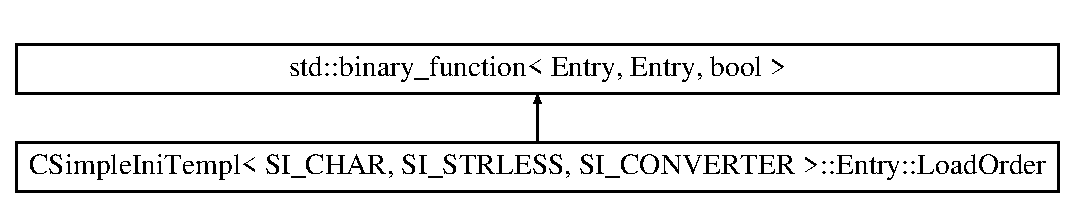
\includegraphics[height=2.000000cm]{a01395}
\end{center}
\end{figure}
\subsection*{Public Member Functions}
\begin{DoxyCompactItemize}
\item 
\mbox{\Hypertarget{a01395_a51113d39d0dd9c36819d5b3dda2ac148}\label{a01395_a51113d39d0dd9c36819d5b3dda2ac148}} 
bool {\bfseries operator()} (const \hyperlink{a01387}{Entry} \&lhs, const \hyperlink{a01387}{Entry} \&rhs) const
\end{DoxyCompactItemize}


\subsection{Detailed Description}
\subsubsection*{template$<$class S\+I\+\_\+\+C\+H\+AR, class S\+I\+\_\+\+S\+T\+R\+L\+E\+SS, class S\+I\+\_\+\+C\+O\+N\+V\+E\+R\+T\+ER$>$\newline
struct C\+Simple\+Ini\+Templ$<$ S\+I\+\_\+\+C\+H\+A\+R, S\+I\+\_\+\+S\+T\+R\+L\+E\+S\+S, S\+I\+\_\+\+C\+O\+N\+V\+E\+R\+T\+E\+R $>$\+::\+Entry\+::\+Load\+Order}

Strict less ordering by order, and then name of key 

The documentation for this struct was generated from the following file\+:\begin{DoxyCompactItemize}
\item 
Simple\+Ini.\+h\end{DoxyCompactItemize}

\hypertarget{a01291}{}\section{fire\+:\+:Local\+Parser$<$ T $>$ Class Template Reference}
\label{a01291}\index{fire\+::\+Local\+Parser$<$ T $>$@{fire\+::\+Local\+Parser$<$ T $>$}}


{\ttfamily \#include $<$Local\+Parser.\+h$>$}

Inheritance diagram for fire\+:\+:Local\+Parser$<$ T $>$\+:\begin{figure}[H]
\begin{center}
\leavevmode
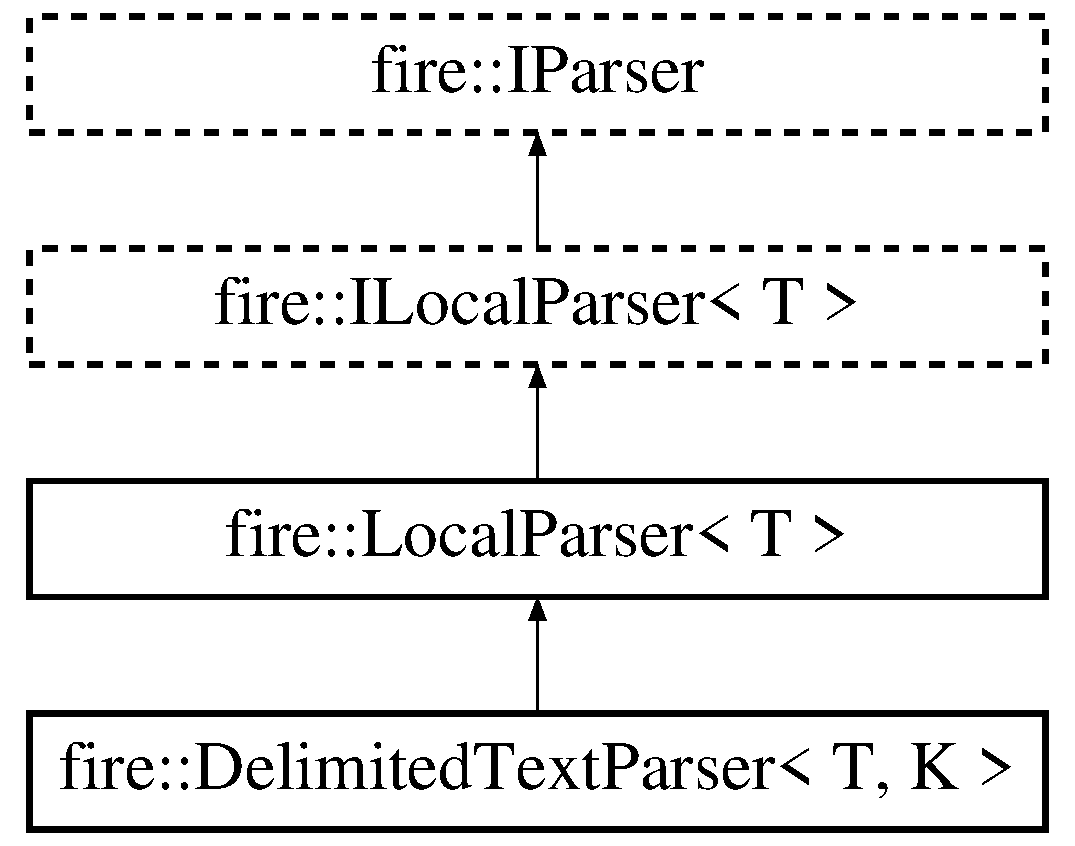
\includegraphics[height=4.000000cm]{a01291}
\end{center}
\end{figure}
\subsection*{Public Member Functions}
\begin{DoxyCompactItemize}
\item 
virtual void \hyperlink{a01291_afcaec6429fdd6e5d53642a32c001ff73}{set\+Source} (const std\+::string \&source)
\item 
virtual void \hyperlink{a01291_abd8929aea06c2dda40256d2e58236650}{parse} ()
\item 
virtual void \hyperlink{a01291_aed4357541f2ff7d46f8846bd07bb3c42}{set\+Source} (const std\+::istream \&source)
\item 
virtual const std\+::string \& \hyperlink{a01291_aedb7fe10911182525a719963b9b56726}{get\+Source} ()
\item 
virtual const std\+::istream \& \hyperlink{a01291_a9bf19a3cc9ae8ac0e6e7a0e7f6212cdc}{get\+Source\+Stream} ()
\item 
virtual std\+::shared\+\_\+ptr$<$ T $>$ \hyperlink{a01291_ab9016cca8e5dca516bb57c6a8e76607a}{get\+Data} ()
\item 
{\footnotesize template$<$$>$ }\\void \hyperlink{a01291_a34fd9ffb0196c612c75b5288ed5e219b}{parse} ()
\item 
{\footnotesize template$<$$>$ }\\void \hyperlink{a01291_ae904e264fe16708b3e434adea59e1b88}{parse} ()
\end{DoxyCompactItemize}
\subsection*{Protected Attributes}
\begin{DoxyCompactItemize}
\item 
std\+::string \hyperlink{a01291_acf921ee916266efe70be5b24bec37fce}{source\+File}
\item 
std\+::shared\+\_\+ptr$<$ T $>$ \hyperlink{a01291_af8f722c7e35378c69e76e4275d384d86}{data}
\end{DoxyCompactItemize}


\subsection{Detailed Description}
\subsubsection*{template$<$typename T$>$\newline
class fire\+::\+Local\+Parser$<$ T $>$}

The Local\+Parser$<$\+T$>$ is a templated parser that provides support for parsing local files of various types based only on the templated type.

This class works through {\itshape Explicit Specialization}, where subclasses are created using concrete types as template arguments instead of through direct inheritance. One important benefit of this approach to the author is that parsing with local files comes uniform and type-\/independent. For example,


\begin{DoxyCode}
LocalParser<UTKAstroNetwork> parser1;
LocalParser<ReacLib> parser2;

\textcolor{comment}{// Other work...}

network = parser1.parse();
rates = parser2.parse();
\end{DoxyCode}


Confer {\itshape C++ Templates\+: The Complete Guide} by Vandervoorde and Josuttis for full details on explicit specialization.

This class always assumes that its source is a file.

F\+I\+X\+M\+E! -\/ Specialization

Subclasses must always be sure that they implement \hyperlink{a01291_abd8929aea06c2dda40256d2e58236650}{parse()} and \hyperlink{a01291_afcaec6429fdd6e5d53642a32c001ff73}{set\+Source()} because default implementations are not provided. 

\subsection{Member Function Documentation}
\mbox{\Hypertarget{a01291_ab9016cca8e5dca516bb57c6a8e76607a}\label{a01291_ab9016cca8e5dca516bb57c6a8e76607a}} 
\index{fire\+::\+Local\+Parser@{fire\+::\+Local\+Parser}!get\+Data@{get\+Data}}
\index{get\+Data@{get\+Data}!fire\+::\+Local\+Parser@{fire\+::\+Local\+Parser}}
\subsubsection{\texorpdfstring{get\+Data()}{getData()}}
{\footnotesize\ttfamily template$<$typename T$>$ \\
virtual std\+::shared\+\_\+ptr$<$T$>$ \hyperlink{a01291}{fire\+::\+Local\+Parser}$<$ T $>$\+::get\+Data (\begin{DoxyParamCaption}{ }\end{DoxyParamCaption})\hspace{0.3cm}{\ttfamily [inline]}, {\ttfamily [virtual]}}

This operation returns a shared pointer to an instance of type T. \begin{DoxyReturn}{Returns}
a shared pointer holding an instance of type T that was parsed from the file. 
\end{DoxyReturn}


Implements \hyperlink{a01275_a0fc1446d106f0ab8daf8744a4bd29a65}{fire\+::\+I\+Local\+Parser$<$ T $>$}.

\mbox{\Hypertarget{a01291_aedb7fe10911182525a719963b9b56726}\label{a01291_aedb7fe10911182525a719963b9b56726}} 
\index{fire\+::\+Local\+Parser@{fire\+::\+Local\+Parser}!get\+Source@{get\+Source}}
\index{get\+Source@{get\+Source}!fire\+::\+Local\+Parser@{fire\+::\+Local\+Parser}}
\subsubsection{\texorpdfstring{get\+Source()}{getSource()}}
{\footnotesize\ttfamily template$<$typename T$>$ \\
virtual const std\+::string\& \hyperlink{a01291}{fire\+::\+Local\+Parser}$<$ T $>$\+::get\+Source (\begin{DoxyParamCaption}{ }\end{DoxyParamCaption})\hspace{0.3cm}{\ttfamily [inline]}, {\ttfamily [virtual]}}

This operation gets the data source for the parser. \begin{DoxyReturn}{Returns}
the name of the source 
\end{DoxyReturn}


Implements \hyperlink{a01283_ab55d2644dfa6d950d1f874e1e02df095}{fire\+::\+I\+Parser}.



Reimplemented in \hyperlink{a01279_ad02c9a530f20a706d7bb2554813e8d3a}{fire\+::\+I\+N\+I\+Property\+Parser}.

\mbox{\Hypertarget{a01291_a9bf19a3cc9ae8ac0e6e7a0e7f6212cdc}\label{a01291_a9bf19a3cc9ae8ac0e6e7a0e7f6212cdc}} 
\index{fire\+::\+Local\+Parser@{fire\+::\+Local\+Parser}!get\+Source\+Stream@{get\+Source\+Stream}}
\index{get\+Source\+Stream@{get\+Source\+Stream}!fire\+::\+Local\+Parser@{fire\+::\+Local\+Parser}}
\subsubsection{\texorpdfstring{get\+Source\+Stream()}{getSourceStream()}}
{\footnotesize\ttfamily template$<$typename T$>$ \\
virtual const std\+::istream\& \hyperlink{a01291}{fire\+::\+Local\+Parser}$<$ T $>$\+::get\+Source\+Stream (\begin{DoxyParamCaption}{ }\end{DoxyParamCaption})\hspace{0.3cm}{\ttfamily [inline]}, {\ttfamily [virtual]}}

This operation gets the data source for the parser as a stream if and only if it was set as such. \begin{DoxyReturn}{Returns}
source the stream of delimited text data 
\end{DoxyReturn}


Implements \hyperlink{a01283_ac94c7a288bf669322b93ba171c43f90e}{fire\+::\+I\+Parser}.

\mbox{\Hypertarget{a01291_a34fd9ffb0196c612c75b5288ed5e219b}\label{a01291_a34fd9ffb0196c612c75b5288ed5e219b}} 
\index{fire\+::\+Local\+Parser@{fire\+::\+Local\+Parser}!parse@{parse}}
\index{parse@{parse}!fire\+::\+Local\+Parser@{fire\+::\+Local\+Parser}}
\subsubsection{\texorpdfstring{parse()}{parse()}\hspace{0.1cm}{\footnotesize\ttfamily [1/3]}}
{\footnotesize\ttfamily template$<$$>$ \\
void \hyperlink{a01291}{fire\+::\+Local\+Parser}$<$ vector$<$ \hyperlink{a01251}{Reaction} $>$ $>$\+::parse (\begin{DoxyParamCaption}{ }\end{DoxyParamCaption})\hspace{0.3cm}{\ttfamily [virtual]}}

This operation parses a file that holds the basic Reaction information for a thermonuclear network. 

Implements \hyperlink{a01283_af36ac6eedd8c27d2f418869193d7d03c}{fire\+::\+I\+Parser}.



Reimplemented in \hyperlink{a01271_a773fa7ed28cb9d8c384ad94bd81fc93f}{fire\+::\+Delimited\+Text\+Parser$<$ T, K $>$}.

\mbox{\Hypertarget{a01291_ae904e264fe16708b3e434adea59e1b88}\label{a01291_ae904e264fe16708b3e434adea59e1b88}} 
\index{fire\+::\+Local\+Parser@{fire\+::\+Local\+Parser}!parse@{parse}}
\index{parse@{parse}!fire\+::\+Local\+Parser@{fire\+::\+Local\+Parser}}
\subsubsection{\texorpdfstring{parse()}{parse()}\hspace{0.1cm}{\footnotesize\ttfamily [2/3]}}
{\footnotesize\ttfamily template$<$$>$ \\
void \hyperlink{a01291}{fire\+::\+Local\+Parser}$<$ std\+::vector$<$ \hyperlink{a01259}{Species} $>$ $>$\+::parse (\begin{DoxyParamCaption}{ }\end{DoxyParamCaption})\hspace{0.3cm}{\ttfamily [virtual]}}

This operation parses a file that holds the basic species information for a thermonuclear network. 

Implements \hyperlink{a01283_af36ac6eedd8c27d2f418869193d7d03c}{fire\+::\+I\+Parser}.



Reimplemented in \hyperlink{a01271_a773fa7ed28cb9d8c384ad94bd81fc93f}{fire\+::\+Delimited\+Text\+Parser$<$ T, K $>$}.

\mbox{\Hypertarget{a01291_abd8929aea06c2dda40256d2e58236650}\label{a01291_abd8929aea06c2dda40256d2e58236650}} 
\index{fire\+::\+Local\+Parser@{fire\+::\+Local\+Parser}!parse@{parse}}
\index{parse@{parse}!fire\+::\+Local\+Parser@{fire\+::\+Local\+Parser}}
\subsubsection{\texorpdfstring{parse()}{parse()}\hspace{0.1cm}{\footnotesize\ttfamily [3/3]}}
{\footnotesize\ttfamily template$<$typename T$>$ \\
virtual void \hyperlink{a01291}{fire\+::\+Local\+Parser}$<$ T $>$\+::parse (\begin{DoxyParamCaption}{ }\end{DoxyParamCaption})\hspace{0.3cm}{\ttfamily [inline]}, {\ttfamily [virtual]}}

This operation directs the parser to parse its source. 

Implements \hyperlink{a01283_af36ac6eedd8c27d2f418869193d7d03c}{fire\+::\+I\+Parser}.



Reimplemented in \hyperlink{a01271_a773fa7ed28cb9d8c384ad94bd81fc93f}{fire\+::\+Delimited\+Text\+Parser$<$ T, K $>$}, \hyperlink{a01271_a686df5548771cae833d5e721442a821a}{fire\+::\+Delimited\+Text\+Parser$<$ T, K $>$}, and \hyperlink{a01279_a31b6bad01e65ed4bb5f1ba297616c641}{fire\+::\+I\+N\+I\+Property\+Parser}.

\mbox{\Hypertarget{a01291_afcaec6429fdd6e5d53642a32c001ff73}\label{a01291_afcaec6429fdd6e5d53642a32c001ff73}} 
\index{fire\+::\+Local\+Parser@{fire\+::\+Local\+Parser}!set\+Source@{set\+Source}}
\index{set\+Source@{set\+Source}!fire\+::\+Local\+Parser@{fire\+::\+Local\+Parser}}
\subsubsection{\texorpdfstring{set\+Source()}{setSource()}\hspace{0.1cm}{\footnotesize\ttfamily [1/2]}}
{\footnotesize\ttfamily template$<$typename T$>$ \\
virtual void \hyperlink{a01291}{fire\+::\+Local\+Parser}$<$ T $>$\+::set\+Source (\begin{DoxyParamCaption}\item[{const std\+::string \&}]{source }\end{DoxyParamCaption})\hspace{0.3cm}{\ttfamily [inline]}, {\ttfamily [virtual]}}

This operation sets the data source for the parser. 
\begin{DoxyParams}{Parameters}
{\em source} & the name of the source that the parser should parse. \\
\hline
\end{DoxyParams}


Implements \hyperlink{a01283_a0dbeff2b9bd8dbfb2aad7a424eef87d1}{fire\+::\+I\+Parser}.



Reimplemented in \hyperlink{a01279_a06793909bc707a69d0c5772b14bc946d}{fire\+::\+I\+N\+I\+Property\+Parser}.

\mbox{\Hypertarget{a01291_aed4357541f2ff7d46f8846bd07bb3c42}\label{a01291_aed4357541f2ff7d46f8846bd07bb3c42}} 
\index{fire\+::\+Local\+Parser@{fire\+::\+Local\+Parser}!set\+Source@{set\+Source}}
\index{set\+Source@{set\+Source}!fire\+::\+Local\+Parser@{fire\+::\+Local\+Parser}}
\subsubsection{\texorpdfstring{set\+Source()}{setSource()}\hspace{0.1cm}{\footnotesize\ttfamily [2/2]}}
{\footnotesize\ttfamily template$<$typename T$>$ \\
virtual void \hyperlink{a01291}{fire\+::\+Local\+Parser}$<$ T $>$\+::set\+Source (\begin{DoxyParamCaption}\item[{const std\+::istream \&}]{source }\end{DoxyParamCaption})\hspace{0.3cm}{\ttfamily [inline]}, {\ttfamily [virtual]}}

This operation sets the data source for the parser using a stream instead of a string. 
\begin{DoxyParams}{Parameters}
{\em source} & the stream of delimited text data \\
\hline
\end{DoxyParams}


Implements \hyperlink{a01283_a7748a633910e9bfc27411d6bd840496b}{fire\+::\+I\+Parser}.



\subsection{Member Data Documentation}
\mbox{\Hypertarget{a01291_af8f722c7e35378c69e76e4275d384d86}\label{a01291_af8f722c7e35378c69e76e4275d384d86}} 
\index{fire\+::\+Local\+Parser@{fire\+::\+Local\+Parser}!data@{data}}
\index{data@{data}!fire\+::\+Local\+Parser@{fire\+::\+Local\+Parser}}
\subsubsection{\texorpdfstring{data}{data}}
{\footnotesize\ttfamily template$<$typename T$>$ \\
std\+::shared\+\_\+ptr$<$T$>$ \hyperlink{a01291}{fire\+::\+Local\+Parser}$<$ T $>$\+::data\hspace{0.3cm}{\ttfamily [protected]}}

The shared pointer to the data set loaded by the \hyperlink{a01291_abd8929aea06c2dda40256d2e58236650}{parse()} operation. \mbox{\Hypertarget{a01291_acf921ee916266efe70be5b24bec37fce}\label{a01291_acf921ee916266efe70be5b24bec37fce}} 
\index{fire\+::\+Local\+Parser@{fire\+::\+Local\+Parser}!source\+File@{source\+File}}
\index{source\+File@{source\+File}!fire\+::\+Local\+Parser@{fire\+::\+Local\+Parser}}
\subsubsection{\texorpdfstring{source\+File}{sourceFile}}
{\footnotesize\ttfamily template$<$typename T$>$ \\
std\+::string \hyperlink{a01291}{fire\+::\+Local\+Parser}$<$ T $>$\+::source\+File\hspace{0.3cm}{\ttfamily [protected]}}

The source file name used if set\+Source(string) is called. 

The documentation for this class was generated from the following file\+:\begin{DoxyCompactItemize}
\item 
Local\+Parser.\+h\end{DoxyCompactItemize}

\hypertarget{a01191}{}\section{xacc\+:\+:quantum\+:\+:Measure Class Reference}
\label{a01191}\index{xacc\+::quantum\+::\+Measure@{xacc\+::quantum\+::\+Measure}}
Inheritance diagram for xacc\+:\+:quantum\+:\+:Measure\+:\begin{figure}[H]
\begin{center}
\leavevmode
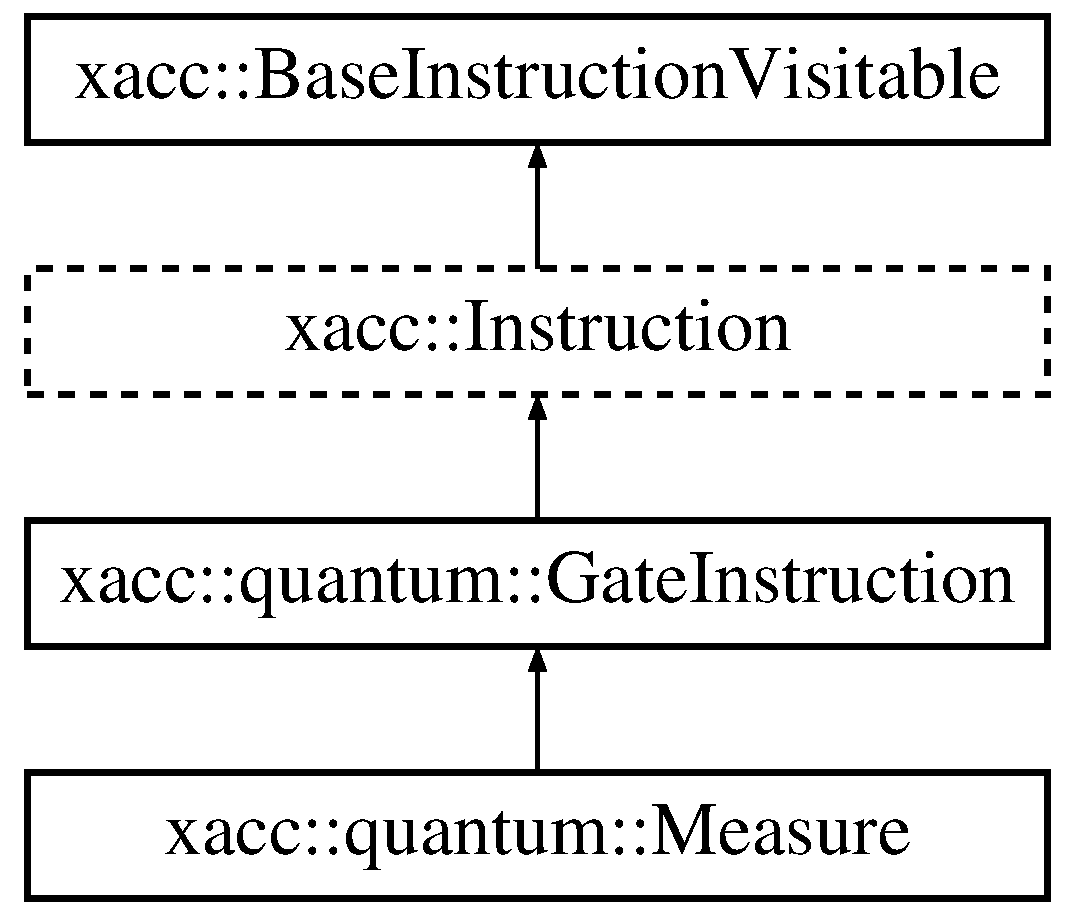
\includegraphics[height=4.000000cm]{a01191}
\end{center}
\end{figure}
\subsection*{Public Member Functions}
\begin{DoxyCompactItemize}
\item 
\mbox{\Hypertarget{a01191_afe330a0eea029d842ff9c88a817dcc7d}\label{a01191_afe330a0eea029d842ff9c88a817dcc7d}} 
{\bfseries Measure} (std\+::vector$<$ int $>$ qbit)
\item 
\mbox{\Hypertarget{a01191_a9b8d9edca8ad2c3fb132780200f17335}\label{a01191_a9b8d9edca8ad2c3fb132780200f17335}} 
{\bfseries Measure} (int qbit, int classical\+Idx)
\item 
virtual const std\+::string \hyperlink{a01191_a1c51a5d68294dcb2ba1a9fbea63a730f}{to\+String} (const std\+::string \&buffer\+Var\+Name)
\item 
\mbox{\Hypertarget{a01191_a0cb3c94731544042807236ade36fddd0}\label{a01191_a0cb3c94731544042807236ade36fddd0}} 
int {\bfseries get\+Classical\+Bit\+Index} ()
\end{DoxyCompactItemize}
\subsection*{Additional Inherited Members}


\subsection{Member Function Documentation}
\mbox{\Hypertarget{a01191_a1c51a5d68294dcb2ba1a9fbea63a730f}\label{a01191_a1c51a5d68294dcb2ba1a9fbea63a730f}} 
\index{xacc\+::quantum\+::\+Measure@{xacc\+::quantum\+::\+Measure}!to\+String@{to\+String}}
\index{to\+String@{to\+String}!xacc\+::quantum\+::\+Measure@{xacc\+::quantum\+::\+Measure}}
\subsubsection{\texorpdfstring{to\+String()}{toString()}}
{\footnotesize\ttfamily const std\+::string xacc\+::quantum\+::\+Measure\+::to\+String (\begin{DoxyParamCaption}\item[{const std\+::string \&}]{buffer\+Var\+Name }\end{DoxyParamCaption})\hspace{0.3cm}{\ttfamily [virtual]}}

Return this instruction\textquotesingle{}s assembly-\/like string representation. 
\begin{DoxyParams}{Parameters}
{\em buffer\+Var\+Name} & \\
\hline
\end{DoxyParams}
\begin{DoxyReturn}{Returns}

\end{DoxyReturn}


Reimplemented from \hyperlink{a01159_a089a5da67ff40ac1a6f56e64589822d9}{xacc\+::quantum\+::\+Gate\+Instruction}.



The documentation for this class was generated from the following files\+:\begin{DoxyCompactItemize}
\item 
Measure.\+hpp\item 
Measure.\+cpp\end{DoxyCompactItemize}

\href{https://travis-ci.org/ORNL-QCI/xacc}{\tt }

\section*{X\+A\+CC -\/ e $\ast$$\ast$\+\_\+\+X\+\_\+$\ast$$\ast$ treme-\/scale $\ast$$\ast$\+\_\+\+A\+C\+C\+\_\+$\ast$$\ast$ elerator programming framework}

X\+A\+CC is a programming framework for extreme-\/scale, post-\/exascale accelerator architectures that integrates alongside existing conventional applications. It is a pluggable framework for programming languages developed for next-\/gen computing hardware architectures like quantum and neuromorphic computing. It lets computational scientists efficiently off-\/load classically intractable work to attached accelerators through user-\/friendly Kernel definitions. X\+A\+CC makes post-\/exascale hybrid programming approachable for domain computational scientists.

\subsection*{Documentation }


\begin{DoxyItemize}
\item \href{http://ORNL-QCI.github.io/xacc}{\tt Website and Documentation}
\end{DoxyItemize}

\subsection*{Questions, Bug Reporting, and Issue Tracking }

Questions, bug reporting and issue tracking are provided by Git\+Hub. Please report all bugs by creating a new issue with the bug tag. You can ask questions by creating a new issue with the question tag.

\subsection*{License }

X\+A\+CC has a \mbox{[}B\+SD 3-\/clause open-\/source license\mbox{]}(L\+I\+C\+E\+N\+SE). 
\hypertarget{a01399}{}\section{C\+Simple\+Ini\+Templ$<$ S\+I\+\_\+\+C\+H\+AR, S\+I\+\_\+\+S\+T\+R\+L\+E\+SS, S\+I\+\_\+\+C\+O\+N\+V\+E\+R\+T\+ER $>$\+:\+:Output\+Writer Class Reference}
\label{a01399}\index{C\+Simple\+Ini\+Templ$<$ S\+I\+\_\+\+C\+H\+A\+R, S\+I\+\_\+\+S\+T\+R\+L\+E\+S\+S, S\+I\+\_\+\+C\+O\+N\+V\+E\+R\+T\+E\+R $>$\+::\+Output\+Writer@{C\+Simple\+Ini\+Templ$<$ S\+I\+\_\+\+C\+H\+A\+R, S\+I\+\_\+\+S\+T\+R\+L\+E\+S\+S, S\+I\+\_\+\+C\+O\+N\+V\+E\+R\+T\+E\+R $>$\+::\+Output\+Writer}}


{\ttfamily \#include $<$Simple\+Ini.\+h$>$}

Inheritance diagram for C\+Simple\+Ini\+Templ$<$ S\+I\+\_\+\+C\+H\+AR, S\+I\+\_\+\+S\+T\+R\+L\+E\+SS, S\+I\+\_\+\+C\+O\+N\+V\+E\+R\+T\+ER $>$\+:\+:Output\+Writer\+:\begin{figure}[H]
\begin{center}
\leavevmode
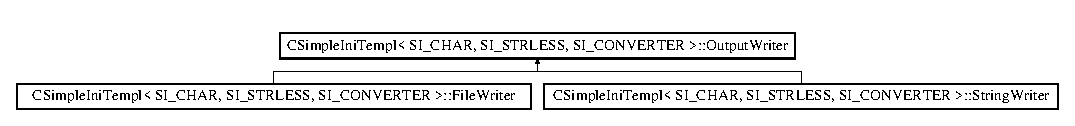
\includegraphics[height=1.244444cm]{a01399}
\end{center}
\end{figure}
\subsection*{Public Member Functions}
\begin{DoxyCompactItemize}
\item 
\mbox{\Hypertarget{a01399_a48e5905a9defbe96d14f3068a383463d}\label{a01399_a48e5905a9defbe96d14f3068a383463d}} 
virtual void {\bfseries Write} (const char $\ast$a\+\_\+p\+Buf)=0
\end{DoxyCompactItemize}


\subsection{Detailed Description}
\subsubsection*{template$<$class S\+I\+\_\+\+C\+H\+AR, class S\+I\+\_\+\+S\+T\+R\+L\+E\+SS, class S\+I\+\_\+\+C\+O\+N\+V\+E\+R\+T\+ER$>$\newline
class C\+Simple\+Ini\+Templ$<$ S\+I\+\_\+\+C\+H\+A\+R, S\+I\+\_\+\+S\+T\+R\+L\+E\+S\+S, S\+I\+\_\+\+C\+O\+N\+V\+E\+R\+T\+E\+R $>$\+::\+Output\+Writer}

interface definition for the \hyperlink{a01399}{Output\+Writer} object to pass to \hyperlink{a01383_a6ec10daab297e92cdffe024ba5e6d999}{Save()} in order to output the I\+NI file data. 

The documentation for this class was generated from the following file\+:\begin{DoxyCompactItemize}
\item 
Simple\+Ini.\+h\end{DoxyCompactItemize}

\hypertarget{a01459}{}\section{xacc\+:\+:Preprocessor Class Reference}
\label{a01459}\index{xacc\+::\+Preprocessor@{xacc\+::\+Preprocessor}}


{\ttfamily \#include $<$Preprocessor.\+hpp$>$}

Inheritance diagram for xacc\+:\+:Preprocessor\+:\begin{figure}[H]
\begin{center}
\leavevmode
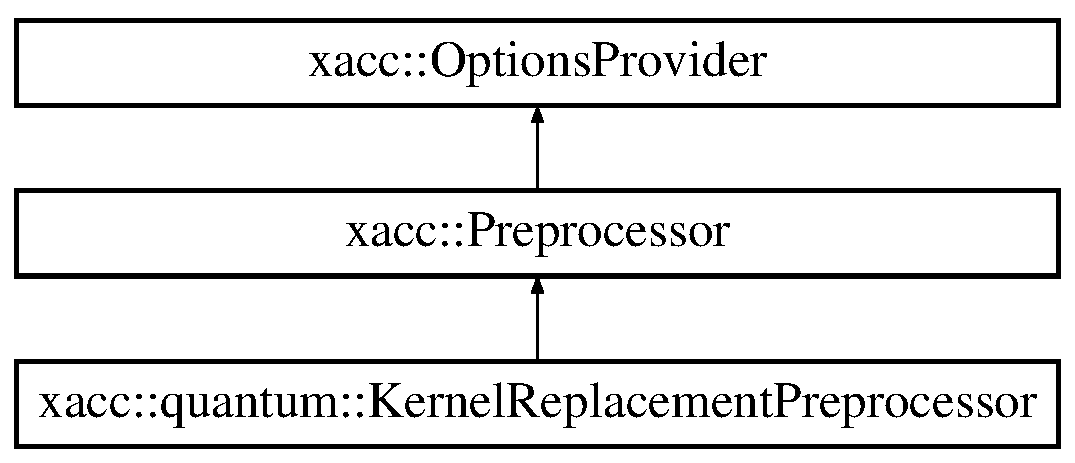
\includegraphics[height=3.000000cm]{a01459}
\end{center}
\end{figure}
\subsection*{Public Member Functions}
\begin{DoxyCompactItemize}
\item 
virtual const std\+::string \hyperlink{a01459_ae59b5a2963f8bcc84b590a83f4749e19}{process} (const std\+::string \&source, std\+::shared\+\_\+ptr$<$ \hyperlink{a01451}{Compiler} $>$ compiler, std\+::shared\+\_\+ptr$<$ \hyperlink{a01435}{Accelerator} $>$ accelerator)=0
\item 
virtual const std\+::string \hyperlink{a01459_a36671f4c062d61e230306edc404774cd}{get\+Name} ()=0
\item 
virtual std\+::shared\+\_\+ptr$<$ options\+\_\+description $>$ \hyperlink{a01459_a96f5600ea47628b66917c7b90250e7f1}{get\+Options} ()
\end{DoxyCompactItemize}


\subsection{Detailed Description}
The \hyperlink{a01459}{Preprocessor} interface provides a mechanism for processing quantum kernel source code before compilation takes place. Realizations of this interface implement the process method which takes as input the source code to process, and the compiler and accelerator this code is targeted at. 

\subsection{Member Function Documentation}
\mbox{\Hypertarget{a01459_a36671f4c062d61e230306edc404774cd}\label{a01459_a36671f4c062d61e230306edc404774cd}} 
\index{xacc\+::\+Preprocessor@{xacc\+::\+Preprocessor}!get\+Name@{get\+Name}}
\index{get\+Name@{get\+Name}!xacc\+::\+Preprocessor@{xacc\+::\+Preprocessor}}
\subsubsection{\texorpdfstring{get\+Name()}{getName()}}
{\footnotesize\ttfamily virtual const std\+::string xacc\+::\+Preprocessor\+::get\+Name (\begin{DoxyParamCaption}{ }\end{DoxyParamCaption})\hspace{0.3cm}{\ttfamily [pure virtual]}}

Return the name of this \hyperlink{a01459}{Preprocessor}

\begin{DoxyReturn}{Returns}
name The name of this preprocessor 
\end{DoxyReturn}


Implemented in \hyperlink{a01135_af74db6b7f3adeb7d203777f5ce450491}{xacc\+::quantum\+::\+Kernel\+Replacement\+Preprocessor}.

\mbox{\Hypertarget{a01459_a96f5600ea47628b66917c7b90250e7f1}\label{a01459_a96f5600ea47628b66917c7b90250e7f1}} 
\index{xacc\+::\+Preprocessor@{xacc\+::\+Preprocessor}!get\+Options@{get\+Options}}
\index{get\+Options@{get\+Options}!xacc\+::\+Preprocessor@{xacc\+::\+Preprocessor}}
\subsubsection{\texorpdfstring{get\+Options()}{getOptions()}}
{\footnotesize\ttfamily virtual std\+::shared\+\_\+ptr$<$options\+\_\+description$>$ xacc\+::\+Preprocessor\+::get\+Options (\begin{DoxyParamCaption}{ }\end{DoxyParamCaption})\hspace{0.3cm}{\ttfamily [inline]}, {\ttfamily [virtual]}}

Return an empty options\+\_\+description, this is for subclasses to implement. 

Implements \hyperlink{a01543_a6d150954f852109bfe2c1ae90222926f}{xacc\+::\+Options\+Provider}.

\mbox{\Hypertarget{a01459_ae59b5a2963f8bcc84b590a83f4749e19}\label{a01459_ae59b5a2963f8bcc84b590a83f4749e19}} 
\index{xacc\+::\+Preprocessor@{xacc\+::\+Preprocessor}!process@{process}}
\index{process@{process}!xacc\+::\+Preprocessor@{xacc\+::\+Preprocessor}}
\subsubsection{\texorpdfstring{process()}{process()}}
{\footnotesize\ttfamily virtual const std\+::string xacc\+::\+Preprocessor\+::process (\begin{DoxyParamCaption}\item[{const std\+::string \&}]{source,  }\item[{std\+::shared\+\_\+ptr$<$ \hyperlink{a01451}{Compiler} $>$}]{compiler,  }\item[{std\+::shared\+\_\+ptr$<$ \hyperlink{a01435}{Accelerator} $>$}]{accelerator }\end{DoxyParamCaption})\hspace{0.3cm}{\ttfamily [pure virtual]}}

This method is to be implemented by subclasses to take in a kernel source string and process it in an isomorphic manner, and returns the processed source code.


\begin{DoxyParams}{Parameters}
{\em src} & The unprocessed kernel source code \\
\hline
{\em compiler} & The compiler being used to compile the code \\
\hline
{\em accelerator} & The \hyperlink{a01435}{Accelerator} this code will be run on\\
\hline
\end{DoxyParams}
\begin{DoxyReturn}{Returns}
processed\+Src The processed kernel source code 
\end{DoxyReturn}


Implemented in \hyperlink{a01135_ad4f9ba1f83ea45ed376f36e3853c668d}{xacc\+::quantum\+::\+Kernel\+Replacement\+Preprocessor}.



The documentation for this class was generated from the following file\+:\begin{DoxyCompactItemize}
\item 
Preprocessor.\+hpp\end{DoxyCompactItemize}

\hypertarget{a01267}{}\section{fire\+:\+:Profile\+Stepper Class Reference}
\label{a01267}\index{fire\+::\+Profile\+Stepper@{fire\+::\+Profile\+Stepper}}


{\ttfamily \#include $<$Profile\+Stepper.\+h$>$}

Inheritance diagram for fire\+:\+:Profile\+Stepper\+:\begin{figure}[H]
\begin{center}
\leavevmode
\includegraphics[height=2.000000cm]{a01267}
\end{center}
\end{figure}
\subsection*{Public Member Functions}
\begin{DoxyCompactItemize}
\item 
\hyperlink{a01267_a5bba5babbcb293b5e6a535cc4d06c55f}{Profile\+Stepper} (const std\+::vector$<$ double $>$ \&steps\+List, const std\+::vector$<$ double $>$ \&step\+Size\+List)
\item 
\hyperlink{a01267_a6838143d952dec2519a43c576a1f1546}{$\sim$\+Profile\+Stepper} ()
\item 
virtual double \hyperlink{a01267_a9096ad65a3fcf63678b600cbe0c33961}{get\+Step} ()
\item 
virtual double \hyperlink{a01267_adaa1a23c068977ecc6809dd8eecab49d}{get\+Step\+Size\+At\+Stage} (int i)
\item 
virtual void \hyperlink{a01267_a2c13fd4da5550f1e58df2b54bbfe4c2c}{update\+Step} ()
\item 
virtual void \hyperlink{a01267_adf2f78648d9539282225117c0fd243af}{set\+Initial\+Step} (double initial\+Step)
\item 
virtual double \hyperlink{a01267_af24660fa4bd027f877d5c1bdeb286cf5}{get\+Initial\+Step} ()
\item 
virtual void \hyperlink{a01267_af8203296b4f3bef53bafab7cb654cc97}{set\+Final\+Step} (double \hyperlink{a01267_a4f2347f039417fe9cdd16d3ca74a072d}{final\+Step})
\item 
virtual double \hyperlink{a01267_ae6f257aca7b3bb62a851169a01bcaacf}{get\+Final\+Step} ()
\item 
virtual void \hyperlink{a01267_a55c44fd97d8b6a474243ad0da48b039d}{set\+Initial\+Stepsize} (double step\+Size)
\item 
virtual double \hyperlink{a01267_a86e7035366907a08a36722655746271e}{get\+Initial\+Stepsize} ()
\end{DoxyCompactItemize}
\subsection*{Protected Attributes}
\begin{DoxyCompactItemize}
\item 
const std\+::vector$<$ double $>$ \& \hyperlink{a01267_a4b388e68798f39795386758f85525cf3}{steps}
\item 
const std\+::vector$<$ double $>$ \& \hyperlink{a01267_a3ab053b93662a362fa16147e88a03c22}{step\+Sizes}
\item 
int \hyperlink{a01267_ac3a3c58d7ff087d09ea71f5f33264853}{step\+ID} = 0
\item 
double \hyperlink{a01267_a4f2347f039417fe9cdd16d3ca74a072d}{final\+Step}
\end{DoxyCompactItemize}


\subsection{Detailed Description}
This class is a Stepper that pulls its steps and step sizes from two matching lists. It can be used for restricting the stepping to a pre-\/determined profile, which is useful for coupling and testing. 

\subsection{Constructor \& Destructor Documentation}
\mbox{\Hypertarget{a01267_a5bba5babbcb293b5e6a535cc4d06c55f}\label{a01267_a5bba5babbcb293b5e6a535cc4d06c55f}} 
\index{fire\+::\+Profile\+Stepper@{fire\+::\+Profile\+Stepper}!Profile\+Stepper@{Profile\+Stepper}}
\index{Profile\+Stepper@{Profile\+Stepper}!fire\+::\+Profile\+Stepper@{fire\+::\+Profile\+Stepper}}
\subsubsection{\texorpdfstring{Profile\+Stepper()}{ProfileStepper()}}
{\footnotesize\ttfamily fire\+::\+Profile\+Stepper\+::\+Profile\+Stepper (\begin{DoxyParamCaption}\item[{const std\+::vector$<$ double $>$ \&}]{steps\+List,  }\item[{const std\+::vector$<$ double $>$ \&}]{step\+Size\+List }\end{DoxyParamCaption})\hspace{0.3cm}{\ttfamily [inline]}}

Constructor \mbox{\Hypertarget{a01267_a6838143d952dec2519a43c576a1f1546}\label{a01267_a6838143d952dec2519a43c576a1f1546}} 
\index{fire\+::\+Profile\+Stepper@{fire\+::\+Profile\+Stepper}!````~Profile\+Stepper@{$\sim$\+Profile\+Stepper}}
\index{````~Profile\+Stepper@{$\sim$\+Profile\+Stepper}!fire\+::\+Profile\+Stepper@{fire\+::\+Profile\+Stepper}}
\subsubsection{\texorpdfstring{$\sim$\+Profile\+Stepper()}{~ProfileStepper()}}
{\footnotesize\ttfamily fire\+::\+Profile\+Stepper\+::$\sim$\+Profile\+Stepper (\begin{DoxyParamCaption}{ }\end{DoxyParamCaption})\hspace{0.3cm}{\ttfamily [inline]}}

Destructor 

\subsection{Member Function Documentation}
\mbox{\Hypertarget{a01267_ae6f257aca7b3bb62a851169a01bcaacf}\label{a01267_ae6f257aca7b3bb62a851169a01bcaacf}} 
\index{fire\+::\+Profile\+Stepper@{fire\+::\+Profile\+Stepper}!get\+Final\+Step@{get\+Final\+Step}}
\index{get\+Final\+Step@{get\+Final\+Step}!fire\+::\+Profile\+Stepper@{fire\+::\+Profile\+Stepper}}
\subsubsection{\texorpdfstring{get\+Final\+Step()}{getFinalStep()}}
{\footnotesize\ttfamily virtual double fire\+::\+Profile\+Stepper\+::get\+Final\+Step (\begin{DoxyParamCaption}{ }\end{DoxyParamCaption})\hspace{0.3cm}{\ttfamily [inline]}, {\ttfamily [virtual]}}

This operation returns the final step for the stepper. \begin{DoxyReturn}{Returns}
the final step 
\end{DoxyReturn}


Implements \hyperlink{a01263_ab234d9f032e02668aededf1c22e8c0a9}{fire\+::\+I\+Stepper}.

\mbox{\Hypertarget{a01267_af24660fa4bd027f877d5c1bdeb286cf5}\label{a01267_af24660fa4bd027f877d5c1bdeb286cf5}} 
\index{fire\+::\+Profile\+Stepper@{fire\+::\+Profile\+Stepper}!get\+Initial\+Step@{get\+Initial\+Step}}
\index{get\+Initial\+Step@{get\+Initial\+Step}!fire\+::\+Profile\+Stepper@{fire\+::\+Profile\+Stepper}}
\subsubsection{\texorpdfstring{get\+Initial\+Step()}{getInitialStep()}}
{\footnotesize\ttfamily virtual double fire\+::\+Profile\+Stepper\+::get\+Initial\+Step (\begin{DoxyParamCaption}{ }\end{DoxyParamCaption})\hspace{0.3cm}{\ttfamily [inline]}, {\ttfamily [virtual]}}

This operation returns the initial step for the stepper. \begin{DoxyReturn}{Returns}
the initial step 
\end{DoxyReturn}


Implements \hyperlink{a01263_a49df3a2ac05cebaf2baf387b66d19272}{fire\+::\+I\+Stepper}.

\mbox{\Hypertarget{a01267_a86e7035366907a08a36722655746271e}\label{a01267_a86e7035366907a08a36722655746271e}} 
\index{fire\+::\+Profile\+Stepper@{fire\+::\+Profile\+Stepper}!get\+Initial\+Stepsize@{get\+Initial\+Stepsize}}
\index{get\+Initial\+Stepsize@{get\+Initial\+Stepsize}!fire\+::\+Profile\+Stepper@{fire\+::\+Profile\+Stepper}}
\subsubsection{\texorpdfstring{get\+Initial\+Stepsize()}{getInitialStepsize()}}
{\footnotesize\ttfamily virtual double fire\+::\+Profile\+Stepper\+::get\+Initial\+Stepsize (\begin{DoxyParamCaption}{ }\end{DoxyParamCaption})\hspace{0.3cm}{\ttfamily [inline]}, {\ttfamily [virtual]}}

This operation gets the initial step size for the stepper \begin{DoxyReturn}{Returns}
the initial step size 
\end{DoxyReturn}


Implements \hyperlink{a01263_afb777e62386b25e5a38d59af54972690}{fire\+::\+I\+Stepper}.

\mbox{\Hypertarget{a01267_a9096ad65a3fcf63678b600cbe0c33961}\label{a01267_a9096ad65a3fcf63678b600cbe0c33961}} 
\index{fire\+::\+Profile\+Stepper@{fire\+::\+Profile\+Stepper}!get\+Step@{get\+Step}}
\index{get\+Step@{get\+Step}!fire\+::\+Profile\+Stepper@{fire\+::\+Profile\+Stepper}}
\subsubsection{\texorpdfstring{get\+Step()}{getStep()}}
{\footnotesize\ttfamily virtual double fire\+::\+Profile\+Stepper\+::get\+Step (\begin{DoxyParamCaption}{ }\end{DoxyParamCaption})\hspace{0.3cm}{\ttfamily [inline]}, {\ttfamily [virtual]}}

This operation returns the step value for the current step. \begin{DoxyReturn}{Returns}
the step value 
\end{DoxyReturn}


Implements \hyperlink{a01263_a7f709d1462a2a3b8bd8214cc681ca26e}{fire\+::\+I\+Stepper}.

\mbox{\Hypertarget{a01267_adaa1a23c068977ecc6809dd8eecab49d}\label{a01267_adaa1a23c068977ecc6809dd8eecab49d}} 
\index{fire\+::\+Profile\+Stepper@{fire\+::\+Profile\+Stepper}!get\+Step\+Size\+At\+Stage@{get\+Step\+Size\+At\+Stage}}
\index{get\+Step\+Size\+At\+Stage@{get\+Step\+Size\+At\+Stage}!fire\+::\+Profile\+Stepper@{fire\+::\+Profile\+Stepper}}
\subsubsection{\texorpdfstring{get\+Step\+Size\+At\+Stage()}{getStepSizeAtStage()}}
{\footnotesize\ttfamily virtual double fire\+::\+Profile\+Stepper\+::get\+Step\+Size\+At\+Stage (\begin{DoxyParamCaption}\item[{int}]{i }\end{DoxyParamCaption})\hspace{0.3cm}{\ttfamily [inline]}, {\ttfamily [virtual]}}

This operation returns the step size for the given stage. 
\begin{DoxyParams}{Parameters}
{\em the} & stage of the solver for which the stepsize should be computed \\
\hline
\end{DoxyParams}
\begin{DoxyReturn}{Returns}
the step size 
\end{DoxyReturn}


Implements \hyperlink{a01263_a43027c0c268afcd59db8815c2e2c41ea}{fire\+::\+I\+Stepper}.

\mbox{\Hypertarget{a01267_af8203296b4f3bef53bafab7cb654cc97}\label{a01267_af8203296b4f3bef53bafab7cb654cc97}} 
\index{fire\+::\+Profile\+Stepper@{fire\+::\+Profile\+Stepper}!set\+Final\+Step@{set\+Final\+Step}}
\index{set\+Final\+Step@{set\+Final\+Step}!fire\+::\+Profile\+Stepper@{fire\+::\+Profile\+Stepper}}
\subsubsection{\texorpdfstring{set\+Final\+Step()}{setFinalStep()}}
{\footnotesize\ttfamily virtual void fire\+::\+Profile\+Stepper\+::set\+Final\+Step (\begin{DoxyParamCaption}\item[{double}]{final\+Step }\end{DoxyParamCaption})\hspace{0.3cm}{\ttfamily [inline]}, {\ttfamily [virtual]}}

This operation sets the final step for the stepper. 
\begin{DoxyParams}{Parameters}
{\em final\+Step} & the final step \\
\hline
\end{DoxyParams}


Implements \hyperlink{a01263_add76974a7b6fbbc93916270a376c461e}{fire\+::\+I\+Stepper}.

\mbox{\Hypertarget{a01267_adf2f78648d9539282225117c0fd243af}\label{a01267_adf2f78648d9539282225117c0fd243af}} 
\index{fire\+::\+Profile\+Stepper@{fire\+::\+Profile\+Stepper}!set\+Initial\+Step@{set\+Initial\+Step}}
\index{set\+Initial\+Step@{set\+Initial\+Step}!fire\+::\+Profile\+Stepper@{fire\+::\+Profile\+Stepper}}
\subsubsection{\texorpdfstring{set\+Initial\+Step()}{setInitialStep()}}
{\footnotesize\ttfamily virtual void fire\+::\+Profile\+Stepper\+::set\+Initial\+Step (\begin{DoxyParamCaption}\item[{double}]{initial\+Step }\end{DoxyParamCaption})\hspace{0.3cm}{\ttfamily [inline]}, {\ttfamily [virtual]}}

This operation sets the initial step for the stepper. 
\begin{DoxyParams}{Parameters}
{\em initial\+Step} & the initial step \\
\hline
\end{DoxyParams}


Implements \hyperlink{a01263_a3a5099cd0f3c874e56c33cb8f13b8f3b}{fire\+::\+I\+Stepper}.

\mbox{\Hypertarget{a01267_a55c44fd97d8b6a474243ad0da48b039d}\label{a01267_a55c44fd97d8b6a474243ad0da48b039d}} 
\index{fire\+::\+Profile\+Stepper@{fire\+::\+Profile\+Stepper}!set\+Initial\+Stepsize@{set\+Initial\+Stepsize}}
\index{set\+Initial\+Stepsize@{set\+Initial\+Stepsize}!fire\+::\+Profile\+Stepper@{fire\+::\+Profile\+Stepper}}
\subsubsection{\texorpdfstring{set\+Initial\+Stepsize()}{setInitialStepsize()}}
{\footnotesize\ttfamily virtual void fire\+::\+Profile\+Stepper\+::set\+Initial\+Stepsize (\begin{DoxyParamCaption}\item[{double}]{step\+Size }\end{DoxyParamCaption})\hspace{0.3cm}{\ttfamily [inline]}, {\ttfamily [virtual]}}

This operation sets the initial step size for the stepper 
\begin{DoxyParams}{Parameters}
{\em the} & initial step size \\
\hline
\end{DoxyParams}


Implements \hyperlink{a01263_a69c262f248511efcd271be1724a41ad9}{fire\+::\+I\+Stepper}.

\mbox{\Hypertarget{a01267_a2c13fd4da5550f1e58df2b54bbfe4c2c}\label{a01267_a2c13fd4da5550f1e58df2b54bbfe4c2c}} 
\index{fire\+::\+Profile\+Stepper@{fire\+::\+Profile\+Stepper}!update\+Step@{update\+Step}}
\index{update\+Step@{update\+Step}!fire\+::\+Profile\+Stepper@{fire\+::\+Profile\+Stepper}}
\subsubsection{\texorpdfstring{update\+Step()}{updateStep()}}
{\footnotesize\ttfamily virtual void fire\+::\+Profile\+Stepper\+::update\+Step (\begin{DoxyParamCaption}{ }\end{DoxyParamCaption})\hspace{0.3cm}{\ttfamily [inline]}, {\ttfamily [virtual]}}

This operation replaces the current step and stepsize with the next step and stepsize values. 

Implements \hyperlink{a01263_a44dfccb90ee5ef6e080b54113c215458}{fire\+::\+I\+Stepper}.



\subsection{Member Data Documentation}
\mbox{\Hypertarget{a01267_a4f2347f039417fe9cdd16d3ca74a072d}\label{a01267_a4f2347f039417fe9cdd16d3ca74a072d}} 
\index{fire\+::\+Profile\+Stepper@{fire\+::\+Profile\+Stepper}!final\+Step@{final\+Step}}
\index{final\+Step@{final\+Step}!fire\+::\+Profile\+Stepper@{fire\+::\+Profile\+Stepper}}
\subsubsection{\texorpdfstring{final\+Step}{finalStep}}
{\footnotesize\ttfamily double fire\+::\+Profile\+Stepper\+::final\+Step\hspace{0.3cm}{\ttfamily [protected]}}

The final step value. \mbox{\Hypertarget{a01267_ac3a3c58d7ff087d09ea71f5f33264853}\label{a01267_ac3a3c58d7ff087d09ea71f5f33264853}} 
\index{fire\+::\+Profile\+Stepper@{fire\+::\+Profile\+Stepper}!step\+ID@{step\+ID}}
\index{step\+ID@{step\+ID}!fire\+::\+Profile\+Stepper@{fire\+::\+Profile\+Stepper}}
\subsubsection{\texorpdfstring{step\+ID}{stepID}}
{\footnotesize\ttfamily int fire\+::\+Profile\+Stepper\+::step\+ID = 0\hspace{0.3cm}{\ttfamily [protected]}}

The id number of the current staff \mbox{\Hypertarget{a01267_a4b388e68798f39795386758f85525cf3}\label{a01267_a4b388e68798f39795386758f85525cf3}} 
\index{fire\+::\+Profile\+Stepper@{fire\+::\+Profile\+Stepper}!steps@{steps}}
\index{steps@{steps}!fire\+::\+Profile\+Stepper@{fire\+::\+Profile\+Stepper}}
\subsubsection{\texorpdfstring{steps}{steps}}
{\footnotesize\ttfamily const std\+::vector$<$double$>$\& fire\+::\+Profile\+Stepper\+::steps\hspace{0.3cm}{\ttfamily [protected]}}

The lists of steps \mbox{\Hypertarget{a01267_a3ab053b93662a362fa16147e88a03c22}\label{a01267_a3ab053b93662a362fa16147e88a03c22}} 
\index{fire\+::\+Profile\+Stepper@{fire\+::\+Profile\+Stepper}!step\+Sizes@{step\+Sizes}}
\index{step\+Sizes@{step\+Sizes}!fire\+::\+Profile\+Stepper@{fire\+::\+Profile\+Stepper}}
\subsubsection{\texorpdfstring{step\+Sizes}{stepSizes}}
{\footnotesize\ttfamily const std\+::vector$<$double$>$\& fire\+::\+Profile\+Stepper\+::step\+Sizes\hspace{0.3cm}{\ttfamily [protected]}}

The list of step sizes -\/ the distances between the steps 

The documentation for this class was generated from the following file\+:\begin{DoxyCompactItemize}
\item 
Profile\+Stepper.\+h\end{DoxyCompactItemize}

\hypertarget{a01507}{}\section{xacc\+:\+:Program Class Reference}
\label{a01507}\index{xacc\+::\+Program@{xacc\+::\+Program}}


{\ttfamily \#include $<$Program.\+hpp$>$}

\subsection*{Public Member Functions}
\begin{DoxyCompactItemize}
\item 
\hyperlink{a01507_a6d20079fde67a3ef145315e762249115}{Program} (std\+::shared\+\_\+ptr$<$ \hyperlink{a01435}{Accelerator} $>$ acc, const std\+::string \&source\+File)
\item 
{\footnotesize template$<$typename ... Runtime\+Args$>$ }\\std\+::function$<$ void(std\+::shared\+\_\+ptr$<$ \hyperlink{a01447}{Accelerator\+Buffer} $>$, Runtime\+Args...)$>$ \hyperlink{a01507_abf5023c9f01cac8a506bdef86760e8f1}{get\+Kernel} (const std\+::string \&kernel\+Name)
\end{DoxyCompactItemize}
\subsection*{Protected Member Functions}
\begin{DoxyCompactItemize}
\item 
void \hyperlink{a01507_a53079c7886c0be065968bcf6674d1516}{build} ()
\end{DoxyCompactItemize}
\subsection*{Protected Attributes}
\begin{DoxyCompactItemize}
\item 
std\+::string \hyperlink{a01507_aae78160f9f9e52a3e0c9b342996a7202}{src}
\item 
std\+::shared\+\_\+ptr$<$ \hyperlink{a01435}{Accelerator} $>$ \hyperlink{a01507_a10c948629c84f23dd426c04a9a518155}{accelerator}
\item 
std\+::shared\+\_\+ptr$<$ \hyperlink{a01499}{IR} $>$ \hyperlink{a01507_a5681f0989fc1c3fced8e30e815d6511c}{xacc\+IR}
\item 
std\+::shared\+\_\+ptr$<$ \hyperlink{a01451}{Compiler} $>$ \hyperlink{a01507_a0d2ae2522bb0daad0eea7871fc4e2061}{compiler}
\end{DoxyCompactItemize}


\subsection{Detailed Description}
The \hyperlink{a01507}{Program} is the main entrypoint for the X\+A\+CC A\+PI. Users with accelerator kernels must construct a valid \hyperlink{a01507}{Program} to be compiled and executed on the attached accelerator. Programs must be given the \hyperlink{a01435}{Accelerator} reference to be used and kernel source code at construction time. 

\subsection{Constructor \& Destructor Documentation}
\mbox{\Hypertarget{a01507_a6d20079fde67a3ef145315e762249115}\label{a01507_a6d20079fde67a3ef145315e762249115}} 
\index{xacc\+::\+Program@{xacc\+::\+Program}!Program@{Program}}
\index{Program@{Program}!xacc\+::\+Program@{xacc\+::\+Program}}
\subsubsection{\texorpdfstring{Program()}{Program()}}
{\footnotesize\ttfamily xacc\+::\+Program\+::\+Program (\begin{DoxyParamCaption}\item[{std\+::shared\+\_\+ptr$<$ \hyperlink{a01435}{Accelerator} $>$}]{acc,  }\item[{const std\+::string \&}]{source\+File }\end{DoxyParamCaption})\hspace{0.3cm}{\ttfamily [inline]}}

The Constructor, takes the \hyperlink{a01435}{Accelerator} to execute on, and the source to compile and execute


\begin{DoxyParams}{Parameters}
{\em acc} & Attached \hyperlink{a01435}{Accelerator} to execute \\
\hline
{\em source\+File} & The kernel source code \\
\hline
\end{DoxyParams}


\subsection{Member Function Documentation}
\mbox{\Hypertarget{a01507_a53079c7886c0be065968bcf6674d1516}\label{a01507_a53079c7886c0be065968bcf6674d1516}} 
\index{xacc\+::\+Program@{xacc\+::\+Program}!build@{build}}
\index{build@{build}!xacc\+::\+Program@{xacc\+::\+Program}}
\subsubsection{\texorpdfstring{build()}{build()}}
{\footnotesize\ttfamily void xacc\+::\+Program\+::build (\begin{DoxyParamCaption}{ }\end{DoxyParamCaption})\hspace{0.3cm}{\ttfamily [inline]}, {\ttfamily [protected]}}

Execute the compilation mechanism on the provided program source kernel code to produce X\+A\+CC \hyperlink{a01499}{IR} that can be executed on the attached \hyperlink{a01435}{Accelerator}. \mbox{\Hypertarget{a01507_abf5023c9f01cac8a506bdef86760e8f1}\label{a01507_abf5023c9f01cac8a506bdef86760e8f1}} 
\index{xacc\+::\+Program@{xacc\+::\+Program}!get\+Kernel@{get\+Kernel}}
\index{get\+Kernel@{get\+Kernel}!xacc\+::\+Program@{xacc\+::\+Program}}
\subsubsection{\texorpdfstring{get\+Kernel()}{getKernel()}}
{\footnotesize\ttfamily template$<$typename ... Runtime\+Args$>$ \\
std\+::function$<$void(std\+::shared\+\_\+ptr$<$\hyperlink{a01447}{Accelerator\+Buffer}$>$, Runtime\+Args...)$>$ xacc\+::\+Program\+::get\+Kernel (\begin{DoxyParamCaption}\item[{const std\+::string \&}]{kernel\+Name }\end{DoxyParamCaption})\hspace{0.3cm}{\ttfamily [inline]}}

Return an executable version of the quantum kernel referenced by the kernel\+Name string.


\begin{DoxyParams}{Parameters}
{\em name} & \\
\hline
{\em args} & \\
\hline
\end{DoxyParams}
\begin{DoxyReturn}{Returns}

\end{DoxyReturn}


\subsection{Member Data Documentation}
\mbox{\Hypertarget{a01507_a10c948629c84f23dd426c04a9a518155}\label{a01507_a10c948629c84f23dd426c04a9a518155}} 
\index{xacc\+::\+Program@{xacc\+::\+Program}!accelerator@{accelerator}}
\index{accelerator@{accelerator}!xacc\+::\+Program@{xacc\+::\+Program}}
\subsubsection{\texorpdfstring{accelerator}{accelerator}}
{\footnotesize\ttfamily std\+::shared\+\_\+ptr$<$\hyperlink{a01435}{Accelerator}$>$ xacc\+::\+Program\+::accelerator\hspace{0.3cm}{\ttfamily [protected]}}

Reference to the attached \hyperlink{a01435}{Accelerator} to use in this compilation and execution \mbox{\Hypertarget{a01507_a0d2ae2522bb0daad0eea7871fc4e2061}\label{a01507_a0d2ae2522bb0daad0eea7871fc4e2061}} 
\index{xacc\+::\+Program@{xacc\+::\+Program}!compiler@{compiler}}
\index{compiler@{compiler}!xacc\+::\+Program@{xacc\+::\+Program}}
\subsubsection{\texorpdfstring{compiler}{compiler}}
{\footnotesize\ttfamily std\+::shared\+\_\+ptr$<$\hyperlink{a01451}{Compiler}$>$ xacc\+::\+Program\+::compiler\hspace{0.3cm}{\ttfamily [protected]}}

Reference to the compiler \mbox{\Hypertarget{a01507_aae78160f9f9e52a3e0c9b342996a7202}\label{a01507_aae78160f9f9e52a3e0c9b342996a7202}} 
\index{xacc\+::\+Program@{xacc\+::\+Program}!src@{src}}
\index{src@{src}!xacc\+::\+Program@{xacc\+::\+Program}}
\subsubsection{\texorpdfstring{src}{src}}
{\footnotesize\ttfamily std\+::string xacc\+::\+Program\+::src\hspace{0.3cm}{\ttfamily [protected]}}

Reference to the source accelerator kernel code to be compiled and executed \mbox{\Hypertarget{a01507_a5681f0989fc1c3fced8e30e815d6511c}\label{a01507_a5681f0989fc1c3fced8e30e815d6511c}} 
\index{xacc\+::\+Program@{xacc\+::\+Program}!xacc\+IR@{xacc\+IR}}
\index{xacc\+IR@{xacc\+IR}!xacc\+::\+Program@{xacc\+::\+Program}}
\subsubsection{\texorpdfstring{xacc\+IR}{xaccIR}}
{\footnotesize\ttfamily std\+::shared\+\_\+ptr$<$\hyperlink{a01499}{IR}$>$ xacc\+::\+Program\+::xacc\+IR\hspace{0.3cm}{\ttfamily [protected]}}

Reference to the X\+A\+CC \hyperlink{a01499}{IR} instance that is created by the \hyperlink{a01451}{Compiler} 

The documentation for this class was generated from the following file\+:\begin{DoxyCompactItemize}
\item 
Program.\+hpp\end{DoxyCompactItemize}

\hypertarget{a01355}{}\section{fire\+:\+:Provider\+Builder Struct Reference}
\label{a01355}\index{fire\+::\+Provider\+Builder@{fire\+::\+Provider\+Builder}}


{\ttfamily \#include $<$Tensor\+Provider.\+hpp$>$}

Inheritance diagram for fire\+:\+:Provider\+Builder\+:\begin{figure}[H]
\begin{center}
\leavevmode
\includegraphics[height=2.000000cm]{a01355}
\end{center}
\end{figure}


\subsection{Detailed Description}
A placeholder to ensure that clients give the \hyperlink{a01347}{Tensor} an appropriate \hyperlink{a01351}{Tensor\+Provider} Builder. 

The documentation for this struct was generated from the following file\+:\begin{DoxyCompactItemize}
\item 
Tensor\+Provider.\+hpp\end{DoxyCompactItemize}

\hypertarget{a01239}{}\section{xacc\+:\+:runtime\+\_\+get\+\_\+func\+\_\+table$<$ Tuple, std\+:\+:index\+\_\+sequence$<$ Indices... $>$ $>$ Struct Template Reference}
\label{a01239}\index{xacc\+::runtime\+\_\+get\+\_\+func\+\_\+table$<$ Tuple, std\+::index\+\_\+sequence$<$ Indices... $>$ $>$@{xacc\+::runtime\+\_\+get\+\_\+func\+\_\+table$<$ Tuple, std\+::index\+\_\+sequence$<$ Indices... $>$ $>$}}
\subsection*{Public Types}
\begin{DoxyCompactItemize}
\item 
\mbox{\Hypertarget{a01239_a1d2e9cd7910527e3c4f0162500f067a7}\label{a01239_a1d2e9cd7910527e3c4f0162500f067a7}} 
using {\bfseries return\+\_\+type} = typename std\+::tuple\+\_\+element$<$ 0, Tuple $>$\+::type \&
\item 
\mbox{\Hypertarget{a01239_afba5cf89694dc07b12aaabf6388a4427}\label{a01239_afba5cf89694dc07b12aaabf6388a4427}} 
using {\bfseries get\+\_\+func\+\_\+ptr} = return\+\_\+type($\ast$)(Tuple \&) noexcept
\end{DoxyCompactItemize}
\subsection*{Static Public Attributes}
\begin{DoxyCompactItemize}
\item 
static constexpr get\+\_\+func\+\_\+ptr {\bfseries table} \mbox{[}std\+::tuple\+\_\+size$<$ Tuple $>$\+::value\mbox{]}
\end{DoxyCompactItemize}


\subsection{Member Data Documentation}
\mbox{\Hypertarget{a01239_a80921470cc04db92bab9127ae768d759}\label{a01239_a80921470cc04db92bab9127ae768d759}} 
\index{xacc\+::runtime\+\_\+get\+\_\+func\+\_\+table$<$ Tuple, std\+::index\+\_\+sequence$<$ Indices... $>$ $>$@{xacc\+::runtime\+\_\+get\+\_\+func\+\_\+table$<$ Tuple, std\+::index\+\_\+sequence$<$ Indices... $>$ $>$}!table@{table}}
\index{table@{table}!xacc\+::runtime\+\_\+get\+\_\+func\+\_\+table$<$ Tuple, std\+::index\+\_\+sequence$<$ Indices... $>$ $>$@{xacc\+::runtime\+\_\+get\+\_\+func\+\_\+table$<$ Tuple, std\+::index\+\_\+sequence$<$ Indices... $>$ $>$}}
\subsubsection{\texorpdfstring{table}{table}}
{\footnotesize\ttfamily template$<$typename Tuple , size\+\_\+t ... Indices$>$ \\
constexpr \hyperlink{a01235}{runtime\+\_\+get\+\_\+func\+\_\+table}$<$ Tuple, std\+::index\+\_\+sequence$<$ Indices... $>$ $>$\+::get\+\_\+func\+\_\+ptr \hyperlink{a01235}{xacc\+::runtime\+\_\+get\+\_\+func\+\_\+table}$<$ Tuple, std\+::index\+\_\+sequence$<$ Indices... $>$ $>$\+::table\hspace{0.3cm}{\ttfamily [static]}}

{\bfseries Initial value\+:}
\begin{DoxyCode}
=\{
        &std::get<Indices>...
    \}
\end{DoxyCode}


The documentation for this struct was generated from the following file\+:\begin{DoxyCompactItemize}
\item 
Utils.\+hpp\end{DoxyCompactItemize}

\hypertarget{a01151}{}\section{xacc\+:\+:quantum\+:\+:Q\+FT Class Reference}
\label{a01151}\index{xacc\+::quantum\+::\+Q\+FT@{xacc\+::quantum\+::\+Q\+FT}}


{\ttfamily \#include $<$Q\+F\+T.\+hpp$>$}

Inheritance diagram for xacc\+:\+:quantum\+:\+:Q\+FT\+:\begin{figure}[H]
\begin{center}
\leavevmode
\includegraphics[height=2.000000cm]{a01151}
\end{center}
\end{figure}
\subsection*{Public Member Functions}
\begin{DoxyCompactItemize}
\item 
virtual std\+::shared\+\_\+ptr$<$ \hyperlink{a01475}{Function} $>$ \hyperlink{a01151_ac093c288bc9fc069464fc3fd2cc0ac21}{generate\+Algorithm} (std\+::vector$<$ int $>$ qubits)
\item 
virtual \hyperlink{a01151_a2f585738386f9a3744498983cd1f094e}{$\sim$\+Q\+FT} ()
\end{DoxyCompactItemize}


\subsection{Detailed Description}
\hyperlink{a01151}{Q\+FT} is a realization of the \hyperlink{a01467}{Algorithm\+Generator} interface that produces an X\+A\+CC \hyperlink{a01499}{IR} representation of the Quantum Fourier Transform.

\begin{DoxyAuthor}{Author}
Alex Mc\+Caskey 
\end{DoxyAuthor}


\subsection{Constructor \& Destructor Documentation}
\mbox{\Hypertarget{a01151_a2f585738386f9a3744498983cd1f094e}\label{a01151_a2f585738386f9a3744498983cd1f094e}} 
\index{xacc\+::quantum\+::\+Q\+FT@{xacc\+::quantum\+::\+Q\+FT}!````~Q\+FT@{$\sim$\+Q\+FT}}
\index{````~Q\+FT@{$\sim$\+Q\+FT}!xacc\+::quantum\+::\+Q\+FT@{xacc\+::quantum\+::\+Q\+FT}}
\subsubsection{\texorpdfstring{$\sim$\+Q\+F\+T()}{~QFT()}}
{\footnotesize\ttfamily virtual xacc\+::quantum\+::\+Q\+F\+T\+::$\sim$\+Q\+FT (\begin{DoxyParamCaption}{ }\end{DoxyParamCaption})\hspace{0.3cm}{\ttfamily [inline]}, {\ttfamily [virtual]}}

The destructor 

\subsection{Member Function Documentation}
\mbox{\Hypertarget{a01151_ac093c288bc9fc069464fc3fd2cc0ac21}\label{a01151_ac093c288bc9fc069464fc3fd2cc0ac21}} 
\index{xacc\+::quantum\+::\+Q\+FT@{xacc\+::quantum\+::\+Q\+FT}!generate\+Algorithm@{generate\+Algorithm}}
\index{generate\+Algorithm@{generate\+Algorithm}!xacc\+::quantum\+::\+Q\+FT@{xacc\+::quantum\+::\+Q\+FT}}
\subsubsection{\texorpdfstring{generate\+Algorithm()}{generateAlgorithm()}}
{\footnotesize\ttfamily std\+::shared\+\_\+ptr$<$ \hyperlink{a01475}{Function} $>$ xacc\+::quantum\+::\+Q\+F\+T\+::generate\+Algorithm (\begin{DoxyParamCaption}\item[{std\+::vector$<$ int $>$}]{qubits }\end{DoxyParamCaption})\hspace{0.3cm}{\ttfamily [virtual]}}

This implementation returns a \hyperlink{a01475}{Function} \hyperlink{a01499}{IR} representation of the quantum fourier transform.


\begin{DoxyParams}{Parameters}
{\em bits} & The bits this algorithm operates on \\
\hline
\end{DoxyParams}
\begin{DoxyReturn}{Returns}
function The algorithm represented as an \hyperlink{a01499}{IR} \hyperlink{a01475}{Function} 
\end{DoxyReturn}


Implements \hyperlink{a01467_a73023c06f0f0c62ad56ab4187b18b096}{xacc\+::\+Algorithm\+Generator}.



The documentation for this class was generated from the following files\+:\begin{DoxyCompactItemize}
\item 
Q\+F\+T.\+hpp\item 
Q\+F\+T.\+cpp\end{DoxyCompactItemize}

\hypertarget{a01243}{}\section{xacc\+:\+:quantum\+:\+:Quantum\+Circuit Class Reference}
\label{a01243}\index{xacc\+::quantum\+::\+Quantum\+Circuit@{xacc\+::quantum\+::\+Quantum\+Circuit}}


{\ttfamily \#include $<$Quantum\+Circuit.\+hpp$>$}

Inheritance diagram for xacc\+:\+:quantum\+:\+:Quantum\+Circuit\+:\begin{figure}[H]
\begin{center}
\leavevmode
\includegraphics[height=2.000000cm]{a01243}
\end{center}
\end{figure}
\subsection*{Public Member Functions}
\begin{DoxyCompactItemize}
\item 
virtual void \hyperlink{a01243_af7a7f4a487d493fe8a4ed1f76cefd731}{read} (std\+::istream \&stream)
\end{DoxyCompactItemize}
\subsection*{Additional Inherited Members}


\subsection{Detailed Description}
The \hyperlink{a01243}{Quantum\+Circuit} is a subclass of \hyperlink{a01535}{Graph} that provides its Vertex template parameter as a \hyperlink{a01167}{Circuit\+Node}. It adds the ability to read Quantum\+Circuits from a graphviz dot file. 

\subsection{Member Function Documentation}
\mbox{\Hypertarget{a01243_af7a7f4a487d493fe8a4ed1f76cefd731}\label{a01243_af7a7f4a487d493fe8a4ed1f76cefd731}} 
\index{xacc\+::quantum\+::\+Quantum\+Circuit@{xacc\+::quantum\+::\+Quantum\+Circuit}!read@{read}}
\index{read@{read}!xacc\+::quantum\+::\+Quantum\+Circuit@{xacc\+::quantum\+::\+Quantum\+Circuit}}
\subsubsection{\texorpdfstring{read()}{read()}}
{\footnotesize\ttfamily virtual void xacc\+::quantum\+::\+Quantum\+Circuit\+::read (\begin{DoxyParamCaption}\item[{std\+::istream \&}]{stream }\end{DoxyParamCaption})\hspace{0.3cm}{\ttfamily [inline]}, {\ttfamily [virtual]}}

Read in a graphviz dot graph from the given input stream. This is left for subclasses.


\begin{DoxyParams}{Parameters}
{\em stream} & \\
\hline
\end{DoxyParams}


Reimplemented from \hyperlink{a01535_abdd3e67dc08c223821d809bc8914164a}{xacc\+::\+Graph$<$ Circuit\+Node $>$}.



The documentation for this class was generated from the following file\+:\begin{DoxyCompactItemize}
\item 
Quantum\+Circuit.\+hpp\end{DoxyCompactItemize}

\hypertarget{a01075}{}\section{xacc\+:\+:quantum\+:\+:Z Class Reference}
\label{a01075}\index{xacc\+::quantum\+::Z@{xacc\+::quantum\+::Z}}
Inheritance diagram for xacc\+:\+:quantum\+:\+:Z\+:\begin{figure}[H]
\begin{center}
\leavevmode
\includegraphics[height=4.000000cm]{a01075}
\end{center}
\end{figure}
\subsection*{Public Member Functions}
\begin{DoxyCompactItemize}
\item 
\mbox{\Hypertarget{a01075_a5f1d311b357faed8c2665fe20cf24aeb}\label{a01075_a5f1d311b357faed8c2665fe20cf24aeb}} 
{\bfseries Z} (std\+::vector$<$ int $>$ qbit)
\item 
\mbox{\Hypertarget{a01075_aa1bb7e533e7595e9ecd06879a2f8d2de}\label{a01075_aa1bb7e533e7595e9ecd06879a2f8d2de}} 
{\bfseries Z} (int qbit)
\end{DoxyCompactItemize}
\subsection*{Additional Inherited Members}


The documentation for this class was generated from the following files\+:\begin{DoxyCompactItemize}
\item 
Z.\+hpp\item 
Z.\+cpp\end{DoxyCompactItemize}

\hypertarget{a01079}{}\section{xacc\+:\+:quantum\+:\+:Quil\+Visitor Class Reference}
\label{a01079}\index{xacc\+::quantum\+::\+Quil\+Visitor@{xacc\+::quantum\+::\+Quil\+Visitor}}


{\ttfamily \#include $<$Quil\+Visitor.\+hpp$>$}

Inheritance diagram for xacc\+:\+:quantum\+:\+:Quil\+Visitor\+:\begin{figure}[H]
\begin{center}
\leavevmode
\includegraphics[height=12.000000cm]{a01079}
\end{center}
\end{figure}
\subsection*{Public Member Functions}
\begin{DoxyCompactItemize}
\item 
void \hyperlink{a01079_a5470d573fdcfd691c100fcbfeeed45db}{visit} (\hyperlink{a01187}{Hadamard} \&h)
\item 
void \hyperlink{a01079_ac51ed9d947d3fa00525eb79b2bbc9021}{visit} (\hyperlink{a01175}{C\+N\+OT} \&cn)
\item 
void \hyperlink{a01079_a0b1a31a900f87a3f91f640ab5caec126}{visit} (\hyperlink{a01211}{X} \&x)
\item 
\mbox{\Hypertarget{a01079_a403f2d506425ee5a0098b1b54de7e4e8}\label{a01079_a403f2d506425ee5a0098b1b54de7e4e8}} 
void {\bfseries visit} (\hyperlink{a01215}{Y} \&y)
\item 
void \hyperlink{a01079_af429121067a397eeac17328fc0244859}{visit} (\hyperlink{a01219}{Z} \&z)
\item 
void \hyperlink{a01079_acbe2afe1c9741112d1f9196681f8b896}{visit} (\hyperlink{a01191}{Measure} \&m)
\item 
void \hyperlink{a01079_a7665ecdf9984374f52d30d7767649cf9}{visit} (\hyperlink{a01179}{Conditional\+Function} \&c)
\item 
\mbox{\Hypertarget{a01079_a81a75fb24d368aeb8396d2cbde0bbfb4}\label{a01079_a81a75fb24d368aeb8396d2cbde0bbfb4}} 
void {\bfseries visit} (\hyperlink{a01195}{Rx} \&rx)
\item 
\mbox{\Hypertarget{a01079_ad74c7ec734670c2a5478ebb40e097bfc}\label{a01079_ad74c7ec734670c2a5478ebb40e097bfc}} 
void {\bfseries visit} (\hyperlink{a01199}{Ry} \&ry)
\item 
\mbox{\Hypertarget{a01079_aa3823bdeb4d930f753d4b421730c5912}\label{a01079_aa3823bdeb4d930f753d4b421730c5912}} 
void {\bfseries visit} (\hyperlink{a01203}{Rz} \&rz)
\item 
\mbox{\Hypertarget{a01079_a7a043f72038fec08ac64d375a663e96d}\label{a01079_a7a043f72038fec08ac64d375a663e96d}} 
void {\bfseries visit} (\hyperlink{a01183}{C\+Phase} \&cp)
\item 
\mbox{\Hypertarget{a01079_a2b822a63888043498203dd0b0c935a51}\label{a01079_a2b822a63888043498203dd0b0c935a51}} 
void {\bfseries visit} (\hyperlink{a01207}{Swap} \&s)
\item 
\mbox{\Hypertarget{a01079_addedb7635dd200885904611e4cae39d4}\label{a01079_addedb7635dd200885904611e4cae39d4}} 
void {\bfseries visit} (\hyperlink{a01155}{Gate\+Function} \&f)
\item 
std\+::string \hyperlink{a01079_a9808ecc5766ea2c387107dff6b64cdb8}{get\+Quil\+String} ()
\item 
std\+::string \hyperlink{a01079_ab4a1c6a92772a09c22068ced7d3dc76c}{get\+Classical\+Addresses} ()
\item 
\mbox{\Hypertarget{a01079_a561aabf6de48ae9aee4fbe868f1c5da1}\label{a01079_a561aabf6de48ae9aee4fbe868f1c5da1}} 
int {\bfseries get\+Number\+Of\+Addresses} ()
\item 
virtual \hyperlink{a01079_a90dcced4e75c7b45c287fb4edc58ed01}{$\sim$\+Quil\+Visitor} ()
\end{DoxyCompactItemize}
\subsection*{Protected Attributes}
\begin{DoxyCompactItemize}
\item 
std\+::string \hyperlink{a01079_afd04300ce4dab03448a09f9bee448ca6}{quil\+Str}
\item 
std\+::string \hyperlink{a01079_a93e648797062568ff2ae0345f8843ddd}{classical\+Addresses}
\item 
\mbox{\Hypertarget{a01079_abc613802d6ea40a54c6e75df227a28bb}\label{a01079_abc613802d6ea40a54c6e75df227a28bb}} 
std\+::map$<$ int, int $>$ {\bfseries qubit\+To\+Classical\+Bit\+Index}
\item 
\mbox{\Hypertarget{a01079_ada92b9a834de74d79c22e1c5e88509ec}\label{a01079_ada92b9a834de74d79c22e1c5e88509ec}} 
int {\bfseries num\+Addresses} = 0
\end{DoxyCompactItemize}


\subsection{Detailed Description}
The \hyperlink{a01079}{Quil\+Visitor} is an \hyperlink{a01491}{Instruction\+Visitor} that visits quantum gate instructions and creates an equivalent Quil string that can be executed by the Rigetti superconducting quantum computer. 

\subsection{Constructor \& Destructor Documentation}
\mbox{\Hypertarget{a01079_a90dcced4e75c7b45c287fb4edc58ed01}\label{a01079_a90dcced4e75c7b45c287fb4edc58ed01}} 
\index{xacc\+::quantum\+::\+Quil\+Visitor@{xacc\+::quantum\+::\+Quil\+Visitor}!````~Quil\+Visitor@{$\sim$\+Quil\+Visitor}}
\index{````~Quil\+Visitor@{$\sim$\+Quil\+Visitor}!xacc\+::quantum\+::\+Quil\+Visitor@{xacc\+::quantum\+::\+Quil\+Visitor}}
\subsubsection{\texorpdfstring{$\sim$\+Quil\+Visitor()}{~QuilVisitor()}}
{\footnotesize\ttfamily virtual xacc\+::quantum\+::\+Quil\+Visitor\+::$\sim$\+Quil\+Visitor (\begin{DoxyParamCaption}{ }\end{DoxyParamCaption})\hspace{0.3cm}{\ttfamily [inline]}, {\ttfamily [virtual]}}

The destructor 

\subsection{Member Function Documentation}
\mbox{\Hypertarget{a01079_ab4a1c6a92772a09c22068ced7d3dc76c}\label{a01079_ab4a1c6a92772a09c22068ced7d3dc76c}} 
\index{xacc\+::quantum\+::\+Quil\+Visitor@{xacc\+::quantum\+::\+Quil\+Visitor}!get\+Classical\+Addresses@{get\+Classical\+Addresses}}
\index{get\+Classical\+Addresses@{get\+Classical\+Addresses}!xacc\+::quantum\+::\+Quil\+Visitor@{xacc\+::quantum\+::\+Quil\+Visitor}}
\subsubsection{\texorpdfstring{get\+Classical\+Addresses()}{getClassicalAddresses()}}
{\footnotesize\ttfamily std\+::string xacc\+::quantum\+::\+Quil\+Visitor\+::get\+Classical\+Addresses (\begin{DoxyParamCaption}{ }\end{DoxyParamCaption})\hspace{0.3cm}{\ttfamily [inline]}}

Return the classical measurement indices as a json int array represented as a string. \mbox{\Hypertarget{a01079_a9808ecc5766ea2c387107dff6b64cdb8}\label{a01079_a9808ecc5766ea2c387107dff6b64cdb8}} 
\index{xacc\+::quantum\+::\+Quil\+Visitor@{xacc\+::quantum\+::\+Quil\+Visitor}!get\+Quil\+String@{get\+Quil\+String}}
\index{get\+Quil\+String@{get\+Quil\+String}!xacc\+::quantum\+::\+Quil\+Visitor@{xacc\+::quantum\+::\+Quil\+Visitor}}
\subsubsection{\texorpdfstring{get\+Quil\+String()}{getQuilString()}}
{\footnotesize\ttfamily std\+::string xacc\+::quantum\+::\+Quil\+Visitor\+::get\+Quil\+String (\begin{DoxyParamCaption}{ }\end{DoxyParamCaption})\hspace{0.3cm}{\ttfamily [inline]}}

Return the quil string \mbox{\Hypertarget{a01079_a5470d573fdcfd691c100fcbfeeed45db}\label{a01079_a5470d573fdcfd691c100fcbfeeed45db}} 
\index{xacc\+::quantum\+::\+Quil\+Visitor@{xacc\+::quantum\+::\+Quil\+Visitor}!visit@{visit}}
\index{visit@{visit}!xacc\+::quantum\+::\+Quil\+Visitor@{xacc\+::quantum\+::\+Quil\+Visitor}}
\subsubsection{\texorpdfstring{visit()}{visit()}\hspace{0.1cm}{\footnotesize\ttfamily [1/6]}}
{\footnotesize\ttfamily void xacc\+::quantum\+::\+Quil\+Visitor\+::visit (\begin{DoxyParamCaption}\item[{\hyperlink{a01187}{Hadamard} \&}]{h }\end{DoxyParamCaption})\hspace{0.3cm}{\ttfamily [inline]}}

Visit hadamard gates \mbox{\Hypertarget{a01079_ac51ed9d947d3fa00525eb79b2bbc9021}\label{a01079_ac51ed9d947d3fa00525eb79b2bbc9021}} 
\index{xacc\+::quantum\+::\+Quil\+Visitor@{xacc\+::quantum\+::\+Quil\+Visitor}!visit@{visit}}
\index{visit@{visit}!xacc\+::quantum\+::\+Quil\+Visitor@{xacc\+::quantum\+::\+Quil\+Visitor}}
\subsubsection{\texorpdfstring{visit()}{visit()}\hspace{0.1cm}{\footnotesize\ttfamily [2/6]}}
{\footnotesize\ttfamily void xacc\+::quantum\+::\+Quil\+Visitor\+::visit (\begin{DoxyParamCaption}\item[{\hyperlink{a01175}{C\+N\+OT} \&}]{cn }\end{DoxyParamCaption})\hspace{0.3cm}{\ttfamily [inline]}}

Visit \hyperlink{a01175}{C\+N\+OT} gates \mbox{\Hypertarget{a01079_a0b1a31a900f87a3f91f640ab5caec126}\label{a01079_a0b1a31a900f87a3f91f640ab5caec126}} 
\index{xacc\+::quantum\+::\+Quil\+Visitor@{xacc\+::quantum\+::\+Quil\+Visitor}!visit@{visit}}
\index{visit@{visit}!xacc\+::quantum\+::\+Quil\+Visitor@{xacc\+::quantum\+::\+Quil\+Visitor}}
\subsubsection{\texorpdfstring{visit()}{visit()}\hspace{0.1cm}{\footnotesize\ttfamily [3/6]}}
{\footnotesize\ttfamily void xacc\+::quantum\+::\+Quil\+Visitor\+::visit (\begin{DoxyParamCaption}\item[{\hyperlink{a01211}{X} \&}]{x }\end{DoxyParamCaption})\hspace{0.3cm}{\ttfamily [inline]}}

Visit \hyperlink{a01211}{X} gates \mbox{\Hypertarget{a01079_af429121067a397eeac17328fc0244859}\label{a01079_af429121067a397eeac17328fc0244859}} 
\index{xacc\+::quantum\+::\+Quil\+Visitor@{xacc\+::quantum\+::\+Quil\+Visitor}!visit@{visit}}
\index{visit@{visit}!xacc\+::quantum\+::\+Quil\+Visitor@{xacc\+::quantum\+::\+Quil\+Visitor}}
\subsubsection{\texorpdfstring{visit()}{visit()}\hspace{0.1cm}{\footnotesize\ttfamily [4/6]}}
{\footnotesize\ttfamily void xacc\+::quantum\+::\+Quil\+Visitor\+::visit (\begin{DoxyParamCaption}\item[{\hyperlink{a01219}{Z} \&}]{z }\end{DoxyParamCaption})\hspace{0.3cm}{\ttfamily [inline]}}

Visit \hyperlink{a01219}{Z} gates \mbox{\Hypertarget{a01079_acbe2afe1c9741112d1f9196681f8b896}\label{a01079_acbe2afe1c9741112d1f9196681f8b896}} 
\index{xacc\+::quantum\+::\+Quil\+Visitor@{xacc\+::quantum\+::\+Quil\+Visitor}!visit@{visit}}
\index{visit@{visit}!xacc\+::quantum\+::\+Quil\+Visitor@{xacc\+::quantum\+::\+Quil\+Visitor}}
\subsubsection{\texorpdfstring{visit()}{visit()}\hspace{0.1cm}{\footnotesize\ttfamily [5/6]}}
{\footnotesize\ttfamily void xacc\+::quantum\+::\+Quil\+Visitor\+::visit (\begin{DoxyParamCaption}\item[{\hyperlink{a01191}{Measure} \&}]{m }\end{DoxyParamCaption})\hspace{0.3cm}{\ttfamily [inline]}}

Visit Measurement gates \mbox{\Hypertarget{a01079_a7665ecdf9984374f52d30d7767649cf9}\label{a01079_a7665ecdf9984374f52d30d7767649cf9}} 
\index{xacc\+::quantum\+::\+Quil\+Visitor@{xacc\+::quantum\+::\+Quil\+Visitor}!visit@{visit}}
\index{visit@{visit}!xacc\+::quantum\+::\+Quil\+Visitor@{xacc\+::quantum\+::\+Quil\+Visitor}}
\subsubsection{\texorpdfstring{visit()}{visit()}\hspace{0.1cm}{\footnotesize\ttfamily [6/6]}}
{\footnotesize\ttfamily void xacc\+::quantum\+::\+Quil\+Visitor\+::visit (\begin{DoxyParamCaption}\item[{\hyperlink{a01179}{Conditional\+Function} \&}]{c }\end{DoxyParamCaption})\hspace{0.3cm}{\ttfamily [inline]}}

Visit Conditional functions 

\subsection{Member Data Documentation}
\mbox{\Hypertarget{a01079_a93e648797062568ff2ae0345f8843ddd}\label{a01079_a93e648797062568ff2ae0345f8843ddd}} 
\index{xacc\+::quantum\+::\+Quil\+Visitor@{xacc\+::quantum\+::\+Quil\+Visitor}!classical\+Addresses@{classical\+Addresses}}
\index{classical\+Addresses@{classical\+Addresses}!xacc\+::quantum\+::\+Quil\+Visitor@{xacc\+::quantum\+::\+Quil\+Visitor}}
\subsubsection{\texorpdfstring{classical\+Addresses}{classicalAddresses}}
{\footnotesize\ttfamily std\+::string xacc\+::quantum\+::\+Quil\+Visitor\+::classical\+Addresses\hspace{0.3cm}{\ttfamily [protected]}}

Reference to the classical memory address indices where measurements are recorded. \mbox{\Hypertarget{a01079_afd04300ce4dab03448a09f9bee448ca6}\label{a01079_afd04300ce4dab03448a09f9bee448ca6}} 
\index{xacc\+::quantum\+::\+Quil\+Visitor@{xacc\+::quantum\+::\+Quil\+Visitor}!quil\+Str@{quil\+Str}}
\index{quil\+Str@{quil\+Str}!xacc\+::quantum\+::\+Quil\+Visitor@{xacc\+::quantum\+::\+Quil\+Visitor}}
\subsubsection{\texorpdfstring{quil\+Str}{quilStr}}
{\footnotesize\ttfamily std\+::string xacc\+::quantum\+::\+Quil\+Visitor\+::quil\+Str\hspace{0.3cm}{\ttfamily [protected]}}

Reference to the Quil string this visitor is trying to construct 

The documentation for this class was generated from the following file\+:\begin{DoxyCompactItemize}
\item 
Quil\+Visitor.\+hpp\end{DoxyCompactItemize}

\hypertarget{a01251}{}\section{fire\+:\+:astrophysics\+:\+:Reaction Struct Reference}
\label{a01251}\index{fire\+::astrophysics\+::\+Reaction@{fire\+::astrophysics\+::\+Reaction}}


{\ttfamily \#include $<$Reaction.\+h$>$}

\subsection*{Public Member Functions}
\begin{DoxyCompactItemize}
\item 
void \hyperlink{a01251_a98b03c550c3926cb5c20f8a27a2ee1ed}{set\+Prefactor} (const double \&rho)
\item 
void \hyperlink{a01251_a671a0560e6843664cdae4d724b8645da}{set\+Rate} (array$<$ double, 6 $>$ temp\+Values)
\item 
void \hyperlink{a01251_a598fe411c64ab247e5d4f299b4a59b70}{set\+Rate} (const double \&temp)
\end{DoxyCompactItemize}
\subsection*{Public Attributes}
\begin{DoxyCompactItemize}
\item 
std\+::string \hyperlink{a01251_abb359091e992ad4cb4cde0faacf6021b}{name}
\item 
int \hyperlink{a01251_ab6d29b5c28ef33ea1d9219b70f02d98a}{reaction\+Group\+Class}
\item 
int \hyperlink{a01251_adb666fe2c511b5a5e86ebcd35ba7faa4}{reaction\+Group\+Member\+Index}
\item 
int \hyperlink{a01251_a581b5410f62a299f2262324d6c0199c7}{reaclib\+Class}
\item 
int \hyperlink{a01251_a86154569e16ef396c93cdf97c5eaf5b7}{num\+Reactants}
\item 
int \hyperlink{a01251_aa59b550e5dbdd34c9c563e7dfc2cbc1e}{num\+Products}
\item 
bool \hyperlink{a01251_a84165249a444a64bdfc41531fbe81cc0}{is\+Electron\+Capture}
\item 
bool \hyperlink{a01251_ae161628da753400b3d2256e2d10a02b9}{is\+Reverse}
\item 
double \hyperlink{a01251_a439daff55fecd97cafc96f204570376a}{statistical\+Factor}
\item 
double \hyperlink{a01251_a07f4db35c5d9bca2d5c5fc8529ec3801}{energy\+Release}
\item 
array$<$ double, 7 $>$ \hyperlink{a01251_aa6265e73f4d2c55441caf95e6eb6e656}{reaclib\+Rate\+Coeff}
\item 
array$<$ int, 4 $>$ \hyperlink{a01251_a74b96d4f5ff99d60adfb88b096a7e256}{reactantZ}
\item 
array$<$ int, 4 $>$ \hyperlink{a01251_a831dcae79d4ed842c9bbdf51ebdd137f}{reactantN}
\item 
array$<$ int, 4 $>$ \hyperlink{a01251_a0586d888e1f60d6371239af888f9158b}{productZ}
\item 
array$<$ int, 4 $>$ \hyperlink{a01251_a81251169f8dd972b6cdc285fbc42c331}{productN}
\item 
array$<$ int, 3 $>$ \hyperlink{a01251_ab13b0133b89c6531a1648b696324d804}{reactants}
\item 
array$<$ int, 3 $>$ \hyperlink{a01251_a5d0e77ebec059081aaafa5ba86df4c88}{products}
\item 
double \hyperlink{a01251_a5033228e6305beb4e8dd717d2f088d99}{prefactor}
\item 
double \hyperlink{a01251_a343553d449e3cca261f8ee166fa6b699}{rate}
\end{DoxyCompactItemize}


\subsection{Detailed Description}
This class represents a reaction, and specifically a nuclear reaction in the astrophysical case. This includes both forward reactions and backward (decay) reactions with one to four reacting bodies.

At the moment, this struct has an extremely bad design. However, it is worth noting that this is significantly better than what is currently used. There are several useful optimizations that will be added in time, such as using the \hyperlink{a01259}{Species} class and creating a new reaction group class. 

\subsection{Member Function Documentation}
\mbox{\Hypertarget{a01251_a98b03c550c3926cb5c20f8a27a2ee1ed}\label{a01251_a98b03c550c3926cb5c20f8a27a2ee1ed}} 
\index{fire\+::astrophysics\+::\+Reaction@{fire\+::astrophysics\+::\+Reaction}!set\+Prefactor@{set\+Prefactor}}
\index{set\+Prefactor@{set\+Prefactor}!fire\+::astrophysics\+::\+Reaction@{fire\+::astrophysics\+::\+Reaction}}
\subsubsection{\texorpdfstring{set\+Prefactor()}{setPrefactor()}}
{\footnotesize\ttfamily void fire\+::astrophysics\+::\+Reaction\+::set\+Prefactor (\begin{DoxyParamCaption}\item[{const double \&}]{rho }\end{DoxyParamCaption})\hspace{0.3cm}{\ttfamily [inline]}}

The statistical prefactor that act as constant multipliers on this reaction. \[ p_s = s\rho^{(n_R -1)}. \] 
\begin{DoxyParams}{Parameters}
{\em rho} & the current density \\
\hline
\end{DoxyParams}
\mbox{\Hypertarget{a01251_a671a0560e6843664cdae4d724b8645da}\label{a01251_a671a0560e6843664cdae4d724b8645da}} 
\index{fire\+::astrophysics\+::\+Reaction@{fire\+::astrophysics\+::\+Reaction}!set\+Rate@{set\+Rate}}
\index{set\+Rate@{set\+Rate}!fire\+::astrophysics\+::\+Reaction@{fire\+::astrophysics\+::\+Reaction}}
\subsubsection{\texorpdfstring{set\+Rate()}{setRate()}\hspace{0.1cm}{\footnotesize\ttfamily [1/2]}}
{\footnotesize\ttfamily void fire\+::astrophysics\+::\+Reaction\+::set\+Rate (\begin{DoxyParamCaption}\item[{array$<$ double, 6 $>$}]{temp\+Values }\end{DoxyParamCaption})\hspace{0.3cm}{\ttfamily [inline]}}

This operation computes and sets the reaction rate. This version is optimized to use pre-\/computed temperature values so that the costly exponentiation does not need to be repeated for each reaction if the temperature doesn\textquotesingle{}t change.

The rate is computed by \[ R = p_s*\sum_k R_k \] where \[p_s\] is the prefactor (based on the statistical prefactor) and \[ R_k = \exp(p_1 + \frac{p_2}{T_9} + \frac{p_3}{T_9^{1/3}} + p_{4}T_9^{1/3} + p_{5}T_9 + p_{6}T_9^{5/3} + p_{7}\ln T_9). \]

$T_9$ is the the temperature in units of $10^9$ Kelvin. Note that p1 = reaclib\+Rate\+Coeff\mbox{[}0\mbox{]} since C++ is a zero-\/indexed language.

In general k may be greater than 1 in the summation for the rate, but in this work k = 1 and \[R = R_k\].

See\+: \char`\"{}\+Stars and Stellar Processes\char`\"{}, Mike Guidry, to be published Cambridge University Press.


\begin{DoxyParams}{Parameters}
{\em temp\+Values} & An array of all six temperature values used to compute the rate. \\
\hline
\end{DoxyParams}
\mbox{\Hypertarget{a01251_a598fe411c64ab247e5d4f299b4a59b70}\label{a01251_a598fe411c64ab247e5d4f299b4a59b70}} 
\index{fire\+::astrophysics\+::\+Reaction@{fire\+::astrophysics\+::\+Reaction}!set\+Rate@{set\+Rate}}
\index{set\+Rate@{set\+Rate}!fire\+::astrophysics\+::\+Reaction@{fire\+::astrophysics\+::\+Reaction}}
\subsubsection{\texorpdfstring{set\+Rate()}{setRate()}\hspace{0.1cm}{\footnotesize\ttfamily [2/2]}}
{\footnotesize\ttfamily void fire\+::astrophysics\+::\+Reaction\+::set\+Rate (\begin{DoxyParamCaption}\item[{const double \&}]{temp }\end{DoxyParamCaption})\hspace{0.3cm}{\ttfamily [inline]}}

This operation computes and sets the reaction rate. This version will use the provided temperature to compute all of the temperature coefficients. See the other version of this function for a more efficient version (which this function actually calls).

The rate is computed by \[ R = p_s*\sum_k R_k \] where \[p_s\] is the prefactor (based on the statistical prefactor) and \[ R_k = \exp(p_1 + \frac{p_2}{T_9} + \frac{p_3}{T_9^{1/3}} + p_{4}T_9^{1/3} + p_{5}T_9 + p_{6}T_9^{5/3} + p_{7}\ln T_9). \]

$T_9$ is the the temperature in units of $10^9$ Kelvin. Note that p1 = reaclib\+Rate\+Coeff\mbox{[}0\mbox{]} since C++ is a zero-\/indexed language.

In general k may be greater than 1 in the summation for the rate, but in this work k = 1 and \[R = R_k\].

See\+: \char`\"{}\+Stars and Stellar Processes\char`\"{}, Mike Guidry, to be published Cambridge University Press.


\begin{DoxyParams}{Parameters}
{\em temp} & the temperature \\
\hline
\end{DoxyParams}


\subsection{Member Data Documentation}
\mbox{\Hypertarget{a01251_a07f4db35c5d9bca2d5c5fc8529ec3801}\label{a01251_a07f4db35c5d9bca2d5c5fc8529ec3801}} 
\index{fire\+::astrophysics\+::\+Reaction@{fire\+::astrophysics\+::\+Reaction}!energy\+Release@{energy\+Release}}
\index{energy\+Release@{energy\+Release}!fire\+::astrophysics\+::\+Reaction@{fire\+::astrophysics\+::\+Reaction}}
\subsubsection{\texorpdfstring{energy\+Release}{energyRelease}}
{\footnotesize\ttfamily double fire\+::astrophysics\+::\+Reaction\+::energy\+Release}

The energy released by this reaction in electron volts. \mbox{\Hypertarget{a01251_a84165249a444a64bdfc41531fbe81cc0}\label{a01251_a84165249a444a64bdfc41531fbe81cc0}} 
\index{fire\+::astrophysics\+::\+Reaction@{fire\+::astrophysics\+::\+Reaction}!is\+Electron\+Capture@{is\+Electron\+Capture}}
\index{is\+Electron\+Capture@{is\+Electron\+Capture}!fire\+::astrophysics\+::\+Reaction@{fire\+::astrophysics\+::\+Reaction}}
\subsubsection{\texorpdfstring{is\+Electron\+Capture}{isElectronCapture}}
{\footnotesize\ttfamily bool fire\+::astrophysics\+::\+Reaction\+::is\+Electron\+Capture}

This is flag that designates whether or not the reaction captures an electron. \mbox{\Hypertarget{a01251_ae161628da753400b3d2256e2d10a02b9}\label{a01251_ae161628da753400b3d2256e2d10a02b9}} 
\index{fire\+::astrophysics\+::\+Reaction@{fire\+::astrophysics\+::\+Reaction}!is\+Reverse@{is\+Reverse}}
\index{is\+Reverse@{is\+Reverse}!fire\+::astrophysics\+::\+Reaction@{fire\+::astrophysics\+::\+Reaction}}
\subsubsection{\texorpdfstring{is\+Reverse}{isReverse}}
{\footnotesize\ttfamily bool fire\+::astrophysics\+::\+Reaction\+::is\+Reverse}

True if this reaction is a reverse reaction.

A\+SK M\+I\+K\+E! Why is this set to false by in F\+E\+RN\textquotesingle{}s load\+Reactions operation? \mbox{\Hypertarget{a01251_abb359091e992ad4cb4cde0faacf6021b}\label{a01251_abb359091e992ad4cb4cde0faacf6021b}} 
\index{fire\+::astrophysics\+::\+Reaction@{fire\+::astrophysics\+::\+Reaction}!name@{name}}
\index{name@{name}!fire\+::astrophysics\+::\+Reaction@{fire\+::astrophysics\+::\+Reaction}}
\subsubsection{\texorpdfstring{name}{name}}
{\footnotesize\ttfamily std\+::string fire\+::astrophysics\+::\+Reaction\+::name}

The name, or label, for the reaction. This should be of the form\+: \char`\"{}he4+he4+he4-\/-\/$>$c12\char`\"{} \mbox{\Hypertarget{a01251_aa59b550e5dbdd34c9c563e7dfc2cbc1e}\label{a01251_aa59b550e5dbdd34c9c563e7dfc2cbc1e}} 
\index{fire\+::astrophysics\+::\+Reaction@{fire\+::astrophysics\+::\+Reaction}!num\+Products@{num\+Products}}
\index{num\+Products@{num\+Products}!fire\+::astrophysics\+::\+Reaction@{fire\+::astrophysics\+::\+Reaction}}
\subsubsection{\texorpdfstring{num\+Products}{numProducts}}
{\footnotesize\ttfamily int fire\+::astrophysics\+::\+Reaction\+::num\+Products}

The number of products produced as a result of the reaction. \mbox{\Hypertarget{a01251_a86154569e16ef396c93cdf97c5eaf5b7}\label{a01251_a86154569e16ef396c93cdf97c5eaf5b7}} 
\index{fire\+::astrophysics\+::\+Reaction@{fire\+::astrophysics\+::\+Reaction}!num\+Reactants@{num\+Reactants}}
\index{num\+Reactants@{num\+Reactants}!fire\+::astrophysics\+::\+Reaction@{fire\+::astrophysics\+::\+Reaction}}
\subsubsection{\texorpdfstring{num\+Reactants}{numReactants}}
{\footnotesize\ttfamily int fire\+::astrophysics\+::\+Reaction\+::num\+Reactants}

The number of species in this reaction. \mbox{\Hypertarget{a01251_a5033228e6305beb4e8dd717d2f088d99}\label{a01251_a5033228e6305beb4e8dd717d2f088d99}} 
\index{fire\+::astrophysics\+::\+Reaction@{fire\+::astrophysics\+::\+Reaction}!prefactor@{prefactor}}
\index{prefactor@{prefactor}!fire\+::astrophysics\+::\+Reaction@{fire\+::astrophysics\+::\+Reaction}}
\subsubsection{\texorpdfstring{prefactor}{prefactor}}
{\footnotesize\ttfamily double fire\+::astrophysics\+::\+Reaction\+::prefactor}

The statistical prefactor that act as constant multipliers on this reaction. \[ p_s = s\rho^{(n_R -1)}. \] 
\begin{DoxyParams}{Parameters}
{\em the} & current density \\
\hline
\end{DoxyParams}
\mbox{\Hypertarget{a01251_a81251169f8dd972b6cdc285fbc42c331}\label{a01251_a81251169f8dd972b6cdc285fbc42c331}} 
\index{fire\+::astrophysics\+::\+Reaction@{fire\+::astrophysics\+::\+Reaction}!productN@{productN}}
\index{productN@{productN}!fire\+::astrophysics\+::\+Reaction@{fire\+::astrophysics\+::\+Reaction}}
\subsubsection{\texorpdfstring{productN}{productN}}
{\footnotesize\ttfamily array$<$int, 4$>$ fire\+::astrophysics\+::\+Reaction\+::productN}

The array of neutron numbers for the products in this reaction. \mbox{\Hypertarget{a01251_a5d0e77ebec059081aaafa5ba86df4c88}\label{a01251_a5d0e77ebec059081aaafa5ba86df4c88}} 
\index{fire\+::astrophysics\+::\+Reaction@{fire\+::astrophysics\+::\+Reaction}!products@{products}}
\index{products@{products}!fire\+::astrophysics\+::\+Reaction@{fire\+::astrophysics\+::\+Reaction}}
\subsubsection{\texorpdfstring{products}{products}}
{\footnotesize\ttfamily array$<$int, 3$>$ fire\+::astrophysics\+::\+Reaction\+::products}

The array of products to add to reac\+Vector.

No idea. A\+SK M\+I\+K\+E! This is used by the partial equilibrium code and may be useless for now. \mbox{\Hypertarget{a01251_a0586d888e1f60d6371239af888f9158b}\label{a01251_a0586d888e1f60d6371239af888f9158b}} 
\index{fire\+::astrophysics\+::\+Reaction@{fire\+::astrophysics\+::\+Reaction}!productZ@{productZ}}
\index{productZ@{productZ}!fire\+::astrophysics\+::\+Reaction@{fire\+::astrophysics\+::\+Reaction}}
\subsubsection{\texorpdfstring{productZ}{productZ}}
{\footnotesize\ttfamily array$<$int, 4$>$ fire\+::astrophysics\+::\+Reaction\+::productZ}

The array of atomic numbers for the products in this reaction. \mbox{\Hypertarget{a01251_a343553d449e3cca261f8ee166fa6b699}\label{a01251_a343553d449e3cca261f8ee166fa6b699}} 
\index{fire\+::astrophysics\+::\+Reaction@{fire\+::astrophysics\+::\+Reaction}!rate@{rate}}
\index{rate@{rate}!fire\+::astrophysics\+::\+Reaction@{fire\+::astrophysics\+::\+Reaction}}
\subsubsection{\texorpdfstring{rate}{rate}}
{\footnotesize\ttfamily double fire\+::astrophysics\+::\+Reaction\+::rate}

The reaction rate as described in \hyperlink{a01251_a671a0560e6843664cdae4d724b8645da}{set\+Rate()}. \mbox{\Hypertarget{a01251_a581b5410f62a299f2262324d6c0199c7}\label{a01251_a581b5410f62a299f2262324d6c0199c7}} 
\index{fire\+::astrophysics\+::\+Reaction@{fire\+::astrophysics\+::\+Reaction}!reaclib\+Class@{reaclib\+Class}}
\index{reaclib\+Class@{reaclib\+Class}!fire\+::astrophysics\+::\+Reaction@{fire\+::astrophysics\+::\+Reaction}}
\subsubsection{\texorpdfstring{reaclib\+Class}{reaclibClass}}
{\footnotesize\ttfamily int fire\+::astrophysics\+::\+Reaction\+::reaclib\+Class}

The class of this reaction in the R\+E\+A\+C\+L\+IB rate library. \mbox{\Hypertarget{a01251_aa6265e73f4d2c55441caf95e6eb6e656}\label{a01251_aa6265e73f4d2c55441caf95e6eb6e656}} 
\index{fire\+::astrophysics\+::\+Reaction@{fire\+::astrophysics\+::\+Reaction}!reaclib\+Rate\+Coeff@{reaclib\+Rate\+Coeff}}
\index{reaclib\+Rate\+Coeff@{reaclib\+Rate\+Coeff}!fire\+::astrophysics\+::\+Reaction@{fire\+::astrophysics\+::\+Reaction}}
\subsubsection{\texorpdfstring{reaclib\+Rate\+Coeff}{reaclibRateCoeff}}
{\footnotesize\ttfamily array$<$double,7$>$ fire\+::astrophysics\+::\+Reaction\+::reaclib\+Rate\+Coeff}

The array of R\+E\+A\+C\+L\+IB p-\/coefficients used in the parameterized computation of the rate. The rate is computed by \[ R = p_s*\sum_k R_k \] where \[p_s\] is the prefactor (based on the statistical prefactor) and \[ R_k = \exp(p_1 + \frac{p_2}{T_9} + \frac{p_3}{T_9^{1/3}} + p_{4}T_9^{1/3} + p_{5}T_9 + p_{6}T_9^{5/3} + p_{7}\ln T_9). \]

$T_9$ is the the temperature in units of $10^9$ Kelvin. Note that p1 = reaclib\+Rate\+Coeff\mbox{[}0\mbox{]} since C++ is a zero-\/indexed language.

In general k may be greater than 1 in the summation for the rate, but in this work k = 1 and \[R = R_k\].

See\+: \char`\"{}\+Stars and Stellar Processes\char`\"{}, Mike Guidry, to be published Cambridge University Press. \mbox{\Hypertarget{a01251_a831dcae79d4ed842c9bbdf51ebdd137f}\label{a01251_a831dcae79d4ed842c9bbdf51ebdd137f}} 
\index{fire\+::astrophysics\+::\+Reaction@{fire\+::astrophysics\+::\+Reaction}!reactantN@{reactantN}}
\index{reactantN@{reactantN}!fire\+::astrophysics\+::\+Reaction@{fire\+::astrophysics\+::\+Reaction}}
\subsubsection{\texorpdfstring{reactantN}{reactantN}}
{\footnotesize\ttfamily array$<$int, 4$>$ fire\+::astrophysics\+::\+Reaction\+::reactantN}

The array of neutron numbers for the reactants in this reaction. \mbox{\Hypertarget{a01251_ab13b0133b89c6531a1648b696324d804}\label{a01251_ab13b0133b89c6531a1648b696324d804}} 
\index{fire\+::astrophysics\+::\+Reaction@{fire\+::astrophysics\+::\+Reaction}!reactants@{reactants}}
\index{reactants@{reactants}!fire\+::astrophysics\+::\+Reaction@{fire\+::astrophysics\+::\+Reaction}}
\subsubsection{\texorpdfstring{reactants}{reactants}}
{\footnotesize\ttfamily array$<$int, 3$>$ fire\+::astrophysics\+::\+Reaction\+::reactants}

The array of reactants to subtract from reac\+Vector.

No idea. A\+SK M\+I\+K\+E! This is used by the partial equilibrium code and may be useless for now. \mbox{\Hypertarget{a01251_a74b96d4f5ff99d60adfb88b096a7e256}\label{a01251_a74b96d4f5ff99d60adfb88b096a7e256}} 
\index{fire\+::astrophysics\+::\+Reaction@{fire\+::astrophysics\+::\+Reaction}!reactantZ@{reactantZ}}
\index{reactantZ@{reactantZ}!fire\+::astrophysics\+::\+Reaction@{fire\+::astrophysics\+::\+Reaction}}
\subsubsection{\texorpdfstring{reactantZ}{reactantZ}}
{\footnotesize\ttfamily array$<$int, 4$>$ fire\+::astrophysics\+::\+Reaction\+::reactantZ}

The array of atomic numbers for the reactants in this reaction. \mbox{\Hypertarget{a01251_ab6d29b5c28ef33ea1d9219b70f02d98a}\label{a01251_ab6d29b5c28ef33ea1d9219b70f02d98a}} 
\index{fire\+::astrophysics\+::\+Reaction@{fire\+::astrophysics\+::\+Reaction}!reaction\+Group\+Class@{reaction\+Group\+Class}}
\index{reaction\+Group\+Class@{reaction\+Group\+Class}!fire\+::astrophysics\+::\+Reaction@{fire\+::astrophysics\+::\+Reaction}}
\subsubsection{\texorpdfstring{reaction\+Group\+Class}{reactionGroupClass}}
{\footnotesize\ttfamily int fire\+::astrophysics\+::\+Reaction\+::reaction\+Group\+Class}

The class of this reaction within its reaction group. \mbox{\Hypertarget{a01251_adb666fe2c511b5a5e86ebcd35ba7faa4}\label{a01251_adb666fe2c511b5a5e86ebcd35ba7faa4}} 
\index{fire\+::astrophysics\+::\+Reaction@{fire\+::astrophysics\+::\+Reaction}!reaction\+Group\+Member\+Index@{reaction\+Group\+Member\+Index}}
\index{reaction\+Group\+Member\+Index@{reaction\+Group\+Member\+Index}!fire\+::astrophysics\+::\+Reaction@{fire\+::astrophysics\+::\+Reaction}}
\subsubsection{\texorpdfstring{reaction\+Group\+Member\+Index}{reactionGroupMemberIndex}}
{\footnotesize\ttfamily int fire\+::astrophysics\+::\+Reaction\+::reaction\+Group\+Member\+Index}

The index of this reaction within the reaction group. \mbox{\Hypertarget{a01251_a439daff55fecd97cafc96f204570376a}\label{a01251_a439daff55fecd97cafc96f204570376a}} 
\index{fire\+::astrophysics\+::\+Reaction@{fire\+::astrophysics\+::\+Reaction}!statistical\+Factor@{statistical\+Factor}}
\index{statistical\+Factor@{statistical\+Factor}!fire\+::astrophysics\+::\+Reaction@{fire\+::astrophysics\+::\+Reaction}}
\subsubsection{\texorpdfstring{statistical\+Factor}{statisticalFactor}}
{\footnotesize\ttfamily double fire\+::astrophysics\+::\+Reaction\+::statistical\+Factor}

A statistical factor associated with this reaction that avoids double counting. It also accounts for the sign needed to designate whether or not the population is depleting or increasing. 

The documentation for this struct was generated from the following file\+:\begin{DoxyCompactItemize}
\item 
Reaction.\+h\end{DoxyCompactItemize}

\hypertarget{a01255}{}\section{fire\+:\+:astrophysics\+:\+:Reaction\+Network Class Reference}
\label{a01255}\index{fire\+::astrophysics\+::\+Reaction\+Network@{fire\+::astrophysics\+::\+Reaction\+Network}}


{\ttfamily \#include $<$Reaction\+Network.\+h$>$}

\subsection*{Public Member Functions}
\begin{DoxyCompactItemize}
\item 
\mbox{\Hypertarget{a01255_a66db1b9f2e597f21bce7bcb88b1fbf8f}\label{a01255_a66db1b9f2e597f21bce7bcb88b1fbf8f}} 
double \& {\bfseries operator()} (int i)
\item 
void \hyperlink{a01255_ab4713cafb974ca41bf6a55619e9fd875}{set\+Properties} (const map$<$ string, string $>$ \&props)
\item 
void \hyperlink{a01255_aa9b4de0566ab0b0f148677d8b97e8c49}{load} ()
\item 
void \hyperlink{a01255_aa0c06237ae72e698aee9cf72d0032fd8}{build\+Flux\+Maps} ()
\item 
void \hyperlink{a01255_ac5b97490e667b011b5e2bea92e16f8b7}{compute\+Prefactors} (const double \&rho)
\item 
void \hyperlink{a01255_a3b1fee4e28576c677d7b852e91c6fa98}{compute\+Rates} (const double \&temp)
\item 
void \hyperlink{a01255_a35a05489358c8e1017bbebb75a9c0114}{compute\+Fluxes} ()
\end{DoxyCompactItemize}
\subsection*{Public Attributes}
\begin{DoxyCompactItemize}
\item 
int \hyperlink{a01255_a17ffe8399181590d59d3d339ce867709}{num\+Species}
\item 
int \hyperlink{a01255_ade8f4d9aa1524cbc45809e7943725d59}{num\+Reactions}
\item 
int \hyperlink{a01255_a91f7685b58b70eca227a098717dfe2c5}{num\+Reaction\+Groups}
\item 
double \hyperlink{a01255_ad3d95ecac758ca7efce6376904455123}{mass\+Tol}
\item 
double \hyperlink{a01255_a0bb068c675589e1ad767c1faf2165ed7}{flux\+Frac}
\item 
string \hyperlink{a01255_abcc4209749ecd64d0ab9621210536ade}{network\+File\+Name}
\item 
string \hyperlink{a01255_abb5fbb289b2e40d3b3dcb3695696e2c2}{rate\+File\+Name}
\item 
shared\+\_\+ptr$<$ vector$<$ \hyperlink{a01259}{Species} $>$ $>$ \hyperlink{a01255_ac3811889f4866a29a49ce3a8d0e80cad}{species}
\item 
shared\+\_\+ptr$<$ vector$<$ \hyperlink{a01251}{Reaction} $>$ $>$ \hyperlink{a01255_a32964b6f6a9cb312e722c1478167b7f0}{reactions}
\item 
vector$<$ double $>$ \hyperlink{a01255_af3aa4184f759b2a8babf765667aa6604}{f\+Plus\+Map}
\item 
vector$<$ double $>$ \hyperlink{a01255_a9065be108e95b1604b0d53e2080f0b57}{f\+Minus\+Map}
\item 
vector$<$ double $>$ \hyperlink{a01255_aca9928041359ecf555a63e4f58e80164}{f\+Plus\+Factors}
\item 
vector$<$ double $>$ \hyperlink{a01255_a3aff20108c80e14f9f4d526a08af49de}{f\+Minus\+Factors}
\item 
vector$<$ unsigned short $>$ \hyperlink{a01255_a6682680b1f2975fa8dc1288d3c463693}{f\+Plus\+Maximums}
\item 
vector$<$ unsigned short $>$ \hyperlink{a01255_a4ea51dc9d41bf555592f93bb237e0440}{f\+Minus\+Maximums}
\item 
\mbox{\Hypertarget{a01255_a9309d86802802f33350fbd4fd679fc2b}\label{a01255_a9309d86802802f33350fbd4fd679fc2b}} 
int {\bfseries num\+F\+Plus}
\item 
\mbox{\Hypertarget{a01255_aec06a5e98ef60a1572072c3ad3fa7722}\label{a01255_aec06a5e98ef60a1572072c3ad3fa7722}} 
int {\bfseries num\+F\+Minus}
\end{DoxyCompactItemize}


\subsection{Detailed Description}
This class collects all of the information about a thermonuclear reaction network for astrophysical systems. It includes all species and reaction information and other stateful variable.

The design of this class is not ideal because it exposes public members variables. This design is still an advancement over the original design in F\+E\+RN and is good enough for now. We\textquotesingle{}ll improve it later. 

\subsection{Member Function Documentation}
\mbox{\Hypertarget{a01255_aa0c06237ae72e698aee9cf72d0032fd8}\label{a01255_aa0c06237ae72e698aee9cf72d0032fd8}} 
\index{fire\+::astrophysics\+::\+Reaction\+Network@{fire\+::astrophysics\+::\+Reaction\+Network}!build\+Flux\+Maps@{build\+Flux\+Maps}}
\index{build\+Flux\+Maps@{build\+Flux\+Maps}!fire\+::astrophysics\+::\+Reaction\+Network@{fire\+::astrophysics\+::\+Reaction\+Network}}
\subsubsection{\texorpdfstring{build\+Flux\+Maps()}{buildFluxMaps()}}
{\footnotesize\ttfamily void fire\+::astrophysics\+::\+Reaction\+Network\+::build\+Flux\+Maps (\begin{DoxyParamCaption}{ }\end{DoxyParamCaption})\hspace{0.3cm}{\ttfamily [inline]}}

This operation builds the \char`\"{}flux maps\char`\"{} that map the contributions of each reaction for each species in the network.

This function was originally written as part of the F\+E\+RN code and desperately needs to be refactored. It is has been adapted to use the \hyperlink{a01259}{Species} and \hyperlink{a01251}{Reaction} classes in Fire, but still contains a number of old constructs that have poor performance implications. Likewise, it lacks a sophisticated view of data structures that could greatly increase its speed. It is fine for now because ultimately the formation of the flux maps and numerical prefactors on the R\+HS take up an extremely small amount of computational time compared to the rest of the integration since they are only computed once on initialization of the network. \mbox{\Hypertarget{a01255_a35a05489358c8e1017bbebb75a9c0114}\label{a01255_a35a05489358c8e1017bbebb75a9c0114}} 
\index{fire\+::astrophysics\+::\+Reaction\+Network@{fire\+::astrophysics\+::\+Reaction\+Network}!compute\+Fluxes@{compute\+Fluxes}}
\index{compute\+Fluxes@{compute\+Fluxes}!fire\+::astrophysics\+::\+Reaction\+Network@{fire\+::astrophysics\+::\+Reaction\+Network}}
\subsubsection{\texorpdfstring{compute\+Fluxes()}{computeFluxes()}}
{\footnotesize\ttfamily void fire\+::astrophysics\+::\+Reaction\+Network\+::compute\+Fluxes (\begin{DoxyParamCaption}{ }\end{DoxyParamCaption})\hspace{0.3cm}{\ttfamily [inline]}}

This operation computes the fluxes for the species in the network under the given conditions. The fluxes are stored in the flux member variable on the species itself. \mbox{\Hypertarget{a01255_ac5b97490e667b011b5e2bea92e16f8b7}\label{a01255_ac5b97490e667b011b5e2bea92e16f8b7}} 
\index{fire\+::astrophysics\+::\+Reaction\+Network@{fire\+::astrophysics\+::\+Reaction\+Network}!compute\+Prefactors@{compute\+Prefactors}}
\index{compute\+Prefactors@{compute\+Prefactors}!fire\+::astrophysics\+::\+Reaction\+Network@{fire\+::astrophysics\+::\+Reaction\+Network}}
\subsubsection{\texorpdfstring{compute\+Prefactors()}{computePrefactors()}}
{\footnotesize\ttfamily void fire\+::astrophysics\+::\+Reaction\+Network\+::compute\+Prefactors (\begin{DoxyParamCaption}\item[{const double \&}]{rho }\end{DoxyParamCaption})\hspace{0.3cm}{\ttfamily [inline]}}

This function computes the prefactors for the reaction rates. It is primarily a convenience function for configuring the reactions. The prefactors are stored in the reactions themselves. 
\begin{DoxyParams}{Parameters}
{\em rho} & the current density in units of g/m$^\wedge$3. \\
\hline
\end{DoxyParams}
\mbox{\Hypertarget{a01255_a3b1fee4e28576c677d7b852e91c6fa98}\label{a01255_a3b1fee4e28576c677d7b852e91c6fa98}} 
\index{fire\+::astrophysics\+::\+Reaction\+Network@{fire\+::astrophysics\+::\+Reaction\+Network}!compute\+Rates@{compute\+Rates}}
\index{compute\+Rates@{compute\+Rates}!fire\+::astrophysics\+::\+Reaction\+Network@{fire\+::astrophysics\+::\+Reaction\+Network}}
\subsubsection{\texorpdfstring{compute\+Rates()}{computeRates()}}
{\footnotesize\ttfamily void fire\+::astrophysics\+::\+Reaction\+Network\+::compute\+Rates (\begin{DoxyParamCaption}\item[{const double \&}]{temp }\end{DoxyParamCaption})\hspace{0.3cm}{\ttfamily [inline]}}

This function computers the reaction rates. It is primarily a convenience function for configuring the reactions. The rates are stored in the rate member variable on the reaction itself. 
\begin{DoxyParams}{Parameters}
{\em temp} & the current temperature in units of 10$^\wedge$9 Kelvin. \\
\hline
\end{DoxyParams}
\mbox{\Hypertarget{a01255_aa9b4de0566ab0b0f148677d8b97e8c49}\label{a01255_aa9b4de0566ab0b0f148677d8b97e8c49}} 
\index{fire\+::astrophysics\+::\+Reaction\+Network@{fire\+::astrophysics\+::\+Reaction\+Network}!load@{load}}
\index{load@{load}!fire\+::astrophysics\+::\+Reaction\+Network@{fire\+::astrophysics\+::\+Reaction\+Network}}
\subsubsection{\texorpdfstring{load()}{load()}}
{\footnotesize\ttfamily void fire\+::astrophysics\+::\+Reaction\+Network\+::load (\begin{DoxyParamCaption}{ }\end{DoxyParamCaption})\hspace{0.3cm}{\ttfamily [inline]}}

This operations directs the Network to load the species and reactions from the files provided in the properties list. \mbox{\Hypertarget{a01255_ab4713cafb974ca41bf6a55619e9fd875}\label{a01255_ab4713cafb974ca41bf6a55619e9fd875}} 
\index{fire\+::astrophysics\+::\+Reaction\+Network@{fire\+::astrophysics\+::\+Reaction\+Network}!set\+Properties@{set\+Properties}}
\index{set\+Properties@{set\+Properties}!fire\+::astrophysics\+::\+Reaction\+Network@{fire\+::astrophysics\+::\+Reaction\+Network}}
\subsubsection{\texorpdfstring{set\+Properties()}{setProperties()}}
{\footnotesize\ttfamily void fire\+::astrophysics\+::\+Reaction\+Network\+::set\+Properties (\begin{DoxyParamCaption}\item[{const map$<$ string, string $>$ \&}]{props }\end{DoxyParamCaption})\hspace{0.3cm}{\ttfamily [inline]}}

This operation sets the properties of the network from a map. It is designed to work with property blocks pulled from I\+NI files. It expects the following keys to have values in the map and accepts the default if they do not\+: num\+Species num\+Reactions num\+Reaction\+Groups mass\+Tol flux\+Frac network\+File rate\+File 
\begin{DoxyParams}{Parameters}
{\em props} & the property map \\
\hline
\end{DoxyParams}


\subsection{Member Data Documentation}
\mbox{\Hypertarget{a01255_a0bb068c675589e1ad767c1faf2165ed7}\label{a01255_a0bb068c675589e1ad767c1faf2165ed7}} 
\index{fire\+::astrophysics\+::\+Reaction\+Network@{fire\+::astrophysics\+::\+Reaction\+Network}!flux\+Frac@{flux\+Frac}}
\index{flux\+Frac@{flux\+Frac}!fire\+::astrophysics\+::\+Reaction\+Network@{fire\+::astrophysics\+::\+Reaction\+Network}}
\subsubsection{\texorpdfstring{flux\+Frac}{fluxFrac}}
{\footnotesize\ttfamily double fire\+::astrophysics\+::\+Reaction\+Network\+::flux\+Frac}

A tunable parameter to limit the integration step size based solely on the flux \mbox{\Hypertarget{a01255_a3aff20108c80e14f9f4d526a08af49de}\label{a01255_a3aff20108c80e14f9f4d526a08af49de}} 
\index{fire\+::astrophysics\+::\+Reaction\+Network@{fire\+::astrophysics\+::\+Reaction\+Network}!f\+Minus\+Factors@{f\+Minus\+Factors}}
\index{f\+Minus\+Factors@{f\+Minus\+Factors}!fire\+::astrophysics\+::\+Reaction\+Network@{fire\+::astrophysics\+::\+Reaction\+Network}}
\subsubsection{\texorpdfstring{f\+Minus\+Factors}{fMinusFactors}}
{\footnotesize\ttfamily vector$<$double$>$ fire\+::astrophysics\+::\+Reaction\+Network\+::f\+Minus\+Factors}

The array of size num\+Species$\ast$num\+Reactions that contains the serialized set of numerical factors due to detracting fluxes. \mbox{\Hypertarget{a01255_a9065be108e95b1604b0d53e2080f0b57}\label{a01255_a9065be108e95b1604b0d53e2080f0b57}} 
\index{fire\+::astrophysics\+::\+Reaction\+Network@{fire\+::astrophysics\+::\+Reaction\+Network}!f\+Minus\+Map@{f\+Minus\+Map}}
\index{f\+Minus\+Map@{f\+Minus\+Map}!fire\+::astrophysics\+::\+Reaction\+Network@{fire\+::astrophysics\+::\+Reaction\+Network}}
\subsubsection{\texorpdfstring{f\+Minus\+Map}{fMinusMap}}
{\footnotesize\ttfamily vector$<$double$>$ fire\+::astrophysics\+::\+Reaction\+Network\+::f\+Minus\+Map}

The array of size num\+Species$\ast$num\+Reactions that contains the serialized map of detracting fluxes for each reaction for each species. \mbox{\Hypertarget{a01255_a4ea51dc9d41bf555592f93bb237e0440}\label{a01255_a4ea51dc9d41bf555592f93bb237e0440}} 
\index{fire\+::astrophysics\+::\+Reaction\+Network@{fire\+::astrophysics\+::\+Reaction\+Network}!f\+Minus\+Maximums@{f\+Minus\+Maximums}}
\index{f\+Minus\+Maximums@{f\+Minus\+Maximums}!fire\+::astrophysics\+::\+Reaction\+Network@{fire\+::astrophysics\+::\+Reaction\+Network}}
\subsubsection{\texorpdfstring{f\+Minus\+Maximums}{fMinusMaximums}}
{\footnotesize\ttfamily vector$<$unsigned short$>$ fire\+::astrophysics\+::\+Reaction\+Network\+::f\+Minus\+Maximums}

The array of maximum detracting flux values for each species in the network. (Size = num\+Species) \mbox{\Hypertarget{a01255_aca9928041359ecf555a63e4f58e80164}\label{a01255_aca9928041359ecf555a63e4f58e80164}} 
\index{fire\+::astrophysics\+::\+Reaction\+Network@{fire\+::astrophysics\+::\+Reaction\+Network}!f\+Plus\+Factors@{f\+Plus\+Factors}}
\index{f\+Plus\+Factors@{f\+Plus\+Factors}!fire\+::astrophysics\+::\+Reaction\+Network@{fire\+::astrophysics\+::\+Reaction\+Network}}
\subsubsection{\texorpdfstring{f\+Plus\+Factors}{fPlusFactors}}
{\footnotesize\ttfamily vector$<$double$>$ fire\+::astrophysics\+::\+Reaction\+Network\+::f\+Plus\+Factors}

The array of size num\+Species$\ast$num\+Reactions that contains the serialized set of numerical factors due to contributing fluxes. \mbox{\Hypertarget{a01255_af3aa4184f759b2a8babf765667aa6604}\label{a01255_af3aa4184f759b2a8babf765667aa6604}} 
\index{fire\+::astrophysics\+::\+Reaction\+Network@{fire\+::astrophysics\+::\+Reaction\+Network}!f\+Plus\+Map@{f\+Plus\+Map}}
\index{f\+Plus\+Map@{f\+Plus\+Map}!fire\+::astrophysics\+::\+Reaction\+Network@{fire\+::astrophysics\+::\+Reaction\+Network}}
\subsubsection{\texorpdfstring{f\+Plus\+Map}{fPlusMap}}
{\footnotesize\ttfamily vector$<$double$>$ fire\+::astrophysics\+::\+Reaction\+Network\+::f\+Plus\+Map}

The array of size num\+Species$\ast$num\+Reactions that contains the serialized map of contributing fluxes for each reaction for each species. \mbox{\Hypertarget{a01255_a6682680b1f2975fa8dc1288d3c463693}\label{a01255_a6682680b1f2975fa8dc1288d3c463693}} 
\index{fire\+::astrophysics\+::\+Reaction\+Network@{fire\+::astrophysics\+::\+Reaction\+Network}!f\+Plus\+Maximums@{f\+Plus\+Maximums}}
\index{f\+Plus\+Maximums@{f\+Plus\+Maximums}!fire\+::astrophysics\+::\+Reaction\+Network@{fire\+::astrophysics\+::\+Reaction\+Network}}
\subsubsection{\texorpdfstring{f\+Plus\+Maximums}{fPlusMaximums}}
{\footnotesize\ttfamily vector$<$unsigned short$>$ fire\+::astrophysics\+::\+Reaction\+Network\+::f\+Plus\+Maximums}

The array of maximum contributing flux values for each species in the network. (Size = num\+Species) \mbox{\Hypertarget{a01255_ad3d95ecac758ca7efce6376904455123}\label{a01255_ad3d95ecac758ca7efce6376904455123}} 
\index{fire\+::astrophysics\+::\+Reaction\+Network@{fire\+::astrophysics\+::\+Reaction\+Network}!mass\+Tol@{mass\+Tol}}
\index{mass\+Tol@{mass\+Tol}!fire\+::astrophysics\+::\+Reaction\+Network@{fire\+::astrophysics\+::\+Reaction\+Network}}
\subsubsection{\texorpdfstring{mass\+Tol}{massTol}}
{\footnotesize\ttfamily double fire\+::astrophysics\+::\+Reaction\+Network\+::mass\+Tol}

The mass tolerance for integration in the network \mbox{\Hypertarget{a01255_abcc4209749ecd64d0ab9621210536ade}\label{a01255_abcc4209749ecd64d0ab9621210536ade}} 
\index{fire\+::astrophysics\+::\+Reaction\+Network@{fire\+::astrophysics\+::\+Reaction\+Network}!network\+File\+Name@{network\+File\+Name}}
\index{network\+File\+Name@{network\+File\+Name}!fire\+::astrophysics\+::\+Reaction\+Network@{fire\+::astrophysics\+::\+Reaction\+Network}}
\subsubsection{\texorpdfstring{network\+File\+Name}{networkFileName}}
{\footnotesize\ttfamily string fire\+::astrophysics\+::\+Reaction\+Network\+::network\+File\+Name}

The name of file that contains the species present in the network. \mbox{\Hypertarget{a01255_a91f7685b58b70eca227a098717dfe2c5}\label{a01255_a91f7685b58b70eca227a098717dfe2c5}} 
\index{fire\+::astrophysics\+::\+Reaction\+Network@{fire\+::astrophysics\+::\+Reaction\+Network}!num\+Reaction\+Groups@{num\+Reaction\+Groups}}
\index{num\+Reaction\+Groups@{num\+Reaction\+Groups}!fire\+::astrophysics\+::\+Reaction\+Network@{fire\+::astrophysics\+::\+Reaction\+Network}}
\subsubsection{\texorpdfstring{num\+Reaction\+Groups}{numReactionGroups}}
{\footnotesize\ttfamily int fire\+::astrophysics\+::\+Reaction\+Network\+::num\+Reaction\+Groups}

The number of reaction groups in the network \mbox{\Hypertarget{a01255_ade8f4d9aa1524cbc45809e7943725d59}\label{a01255_ade8f4d9aa1524cbc45809e7943725d59}} 
\index{fire\+::astrophysics\+::\+Reaction\+Network@{fire\+::astrophysics\+::\+Reaction\+Network}!num\+Reactions@{num\+Reactions}}
\index{num\+Reactions@{num\+Reactions}!fire\+::astrophysics\+::\+Reaction\+Network@{fire\+::astrophysics\+::\+Reaction\+Network}}
\subsubsection{\texorpdfstring{num\+Reactions}{numReactions}}
{\footnotesize\ttfamily int fire\+::astrophysics\+::\+Reaction\+Network\+::num\+Reactions}

The number of reactions between the species in the network \mbox{\Hypertarget{a01255_a17ffe8399181590d59d3d339ce867709}\label{a01255_a17ffe8399181590d59d3d339ce867709}} 
\index{fire\+::astrophysics\+::\+Reaction\+Network@{fire\+::astrophysics\+::\+Reaction\+Network}!num\+Species@{num\+Species}}
\index{num\+Species@{num\+Species}!fire\+::astrophysics\+::\+Reaction\+Network@{fire\+::astrophysics\+::\+Reaction\+Network}}
\subsubsection{\texorpdfstring{num\+Species}{numSpecies}}
{\footnotesize\ttfamily int fire\+::astrophysics\+::\+Reaction\+Network\+::num\+Species}

The number of species in the network \mbox{\Hypertarget{a01255_abb5fbb289b2e40d3b3dcb3695696e2c2}\label{a01255_abb5fbb289b2e40d3b3dcb3695696e2c2}} 
\index{fire\+::astrophysics\+::\+Reaction\+Network@{fire\+::astrophysics\+::\+Reaction\+Network}!rate\+File\+Name@{rate\+File\+Name}}
\index{rate\+File\+Name@{rate\+File\+Name}!fire\+::astrophysics\+::\+Reaction\+Network@{fire\+::astrophysics\+::\+Reaction\+Network}}
\subsubsection{\texorpdfstring{rate\+File\+Name}{rateFileName}}
{\footnotesize\ttfamily string fire\+::astrophysics\+::\+Reaction\+Network\+::rate\+File\+Name}

The name of the file that contains the reaction data for the network. \mbox{\Hypertarget{a01255_a32964b6f6a9cb312e722c1478167b7f0}\label{a01255_a32964b6f6a9cb312e722c1478167b7f0}} 
\index{fire\+::astrophysics\+::\+Reaction\+Network@{fire\+::astrophysics\+::\+Reaction\+Network}!reactions@{reactions}}
\index{reactions@{reactions}!fire\+::astrophysics\+::\+Reaction\+Network@{fire\+::astrophysics\+::\+Reaction\+Network}}
\subsubsection{\texorpdfstring{reactions}{reactions}}
{\footnotesize\ttfamily shared\+\_\+ptr$<$vector$<$\hyperlink{a01251}{Reaction}$>$ $>$ fire\+::astrophysics\+::\+Reaction\+Network\+::reactions}

This is the list of reactions in the network. \mbox{\Hypertarget{a01255_ac3811889f4866a29a49ce3a8d0e80cad}\label{a01255_ac3811889f4866a29a49ce3a8d0e80cad}} 
\index{fire\+::astrophysics\+::\+Reaction\+Network@{fire\+::astrophysics\+::\+Reaction\+Network}!species@{species}}
\index{species@{species}!fire\+::astrophysics\+::\+Reaction\+Network@{fire\+::astrophysics\+::\+Reaction\+Network}}
\subsubsection{\texorpdfstring{species}{species}}
{\footnotesize\ttfamily shared\+\_\+ptr$<$vector$<$\hyperlink{a01259}{Species}$>$ $>$ fire\+::astrophysics\+::\+Reaction\+Network\+::species}

This is the list of species in the network. 

The documentation for this class was generated from the following file\+:\begin{DoxyCompactItemize}
\item 
Reaction\+Network.\+h\end{DoxyCompactItemize}

\hypertarget{a01439}{}\section{xacc\+:\+:Register\+Accelerator$<$ T $>$ Class Template Reference}
\label{a01439}\index{xacc\+::\+Register\+Accelerator$<$ T $>$@{xacc\+::\+Register\+Accelerator$<$ T $>$}}


{\ttfamily \#include $<$Accelerator.\+hpp$>$}

\subsection*{Public Member Functions}
\begin{DoxyCompactItemize}
\item 
\mbox{\Hypertarget{a01439_a329df136d447a887e9794ea078d04706}\label{a01439_a329df136d447a887e9794ea078d04706}} 
{\bfseries Register\+Accelerator} (const std\+::string \&name)
\end{DoxyCompactItemize}


\subsection{Detailed Description}
\subsubsection*{template$<$typename T$>$\newline
class xacc\+::\+Register\+Accelerator$<$ T $>$}

\hyperlink{a01439}{Register\+Accelerator} is a convenience class for registering custom derived \hyperlink{a01435}{Accelerator} classes.

Creators of \hyperlink{a01435}{Accelerator} subclasses create an instance of this class with their \hyperlink{a01435}{Accelerator} subclass as the template parameter to register their \hyperlink{a01435}{Accelerator} with X\+A\+CC. This instance must be created in the C\+PP implementation file for the \hyperlink{a01435}{Accelerator} and at global scope. 

The documentation for this class was generated from the following file\+:\begin{DoxyCompactItemize}
\item 
Accelerator.\+hpp\end{DoxyCompactItemize}

\hypertarget{a01471}{}\section{xacc\+:\+:Register\+Algorithm\+Generator$<$ T $>$ Class Template Reference}
\label{a01471}\index{xacc\+::\+Register\+Algorithm\+Generator$<$ T $>$@{xacc\+::\+Register\+Algorithm\+Generator$<$ T $>$}}


{\ttfamily \#include $<$Algorithm\+Generator.\+hpp$>$}

\subsection*{Public Member Functions}
\begin{DoxyCompactItemize}
\item 
\mbox{\Hypertarget{a01471_af439cc4d7c8d6628a979129a5c1411df}\label{a01471_af439cc4d7c8d6628a979129a5c1411df}} 
{\bfseries Register\+Algorithm\+Generator} (const std\+::string \&name)
\end{DoxyCompactItemize}


\subsection{Detailed Description}
\subsubsection*{template$<$typename T$>$\newline
class xacc\+::\+Register\+Algorithm\+Generator$<$ T $>$}

\hyperlink{a01471}{Register\+Algorithm\+Generator} is a convenience class for registering custom derived \hyperlink{a01467}{Algorithm\+Generator} classes.

Creators of \hyperlink{a01467}{Algorithm\+Generator} subclasses create an instance of this class with their \hyperlink{a01467}{Algorithm\+Generator} subclass as the template parameter to register their \hyperlink{a01467}{Algorithm\+Generator} with X\+A\+CC. This instance must be created in the C\+PP implementation file for the \hyperlink{a01467}{Algorithm\+Generator} and at global scope. 

The documentation for this class was generated from the following file\+:\begin{DoxyCompactItemize}
\item 
Algorithm\+Generator.\+hpp\end{DoxyCompactItemize}

\hypertarget{a01455}{}\section{xacc\+:\+:Register\+Compiler$<$ T $>$ Class Template Reference}
\label{a01455}\index{xacc\+::\+Register\+Compiler$<$ T $>$@{xacc\+::\+Register\+Compiler$<$ T $>$}}


{\ttfamily \#include $<$Compiler.\+hpp$>$}

\subsection*{Public Member Functions}
\begin{DoxyCompactItemize}
\item 
\mbox{\Hypertarget{a01455_a41f5c1abd570b3867b9790cdc02f3355}\label{a01455_a41f5c1abd570b3867b9790cdc02f3355}} 
{\bfseries Register\+Compiler} (const std\+::string \&name)
\end{DoxyCompactItemize}


\subsection{Detailed Description}
\subsubsection*{template$<$typename T$>$\newline
class xacc\+::\+Register\+Compiler$<$ T $>$}

\hyperlink{a01455}{Register\+Compiler} is a convenience class for registering custom derived \hyperlink{a01451}{Compiler} classes.

Creators of \hyperlink{a01451}{Compiler} subclasses create an instance of this class with their \hyperlink{a01451}{Compiler} subclass as the template parameter to register their \hyperlink{a01451}{Compiler} with X\+A\+CC. This instance must be created in the C\+PP implementation file for the \hyperlink{a01451}{Compiler} and at global scope. 

The documentation for this class was generated from the following file\+:\begin{DoxyCompactItemize}
\item 
Compiler.\+hpp\end{DoxyCompactItemize}

\hypertarget{a01127}{}\section{xacc\+:\+:Function Class Reference}
\label{a01127}\index{xacc\+::\+Function@{xacc\+::\+Function}}


{\ttfamily \#include $<$Function.\+hpp$>$}

Inheritance diagram for xacc\+:\+:Function\+:\begin{figure}[H]
\begin{center}
\leavevmode
\includegraphics[height=5.000000cm]{a01127}
\end{center}
\end{figure}
\subsection*{Public Member Functions}
\begin{DoxyCompactItemize}
\item 
virtual const int \hyperlink{a01127_a8901985525f59713e14c61713e07c086}{n\+Instructions} ()=0
\item 
virtual Inst\+Ptr \hyperlink{a01127_afa549fc91b5a05f26d8139954a7e0ed5}{get\+Instruction} (const int idx)=0
\item 
virtual std\+::list$<$ Inst\+Ptr $>$ \hyperlink{a01127_aaf80bd3d49113a92b520785572663032}{get\+Instructions} ()=0
\item 
virtual void \hyperlink{a01127_ab6478b09bb28e194bb555b3180737733}{remove\+Instruction} (const int idx)=0
\item 
virtual void \hyperlink{a01127_a2ef6a4923a6734f90f6ee3d94d263af0}{replace\+Instruction} (const int idx, Inst\+Ptr new\+Inst)=0
\item 
virtual void \hyperlink{a01127_acde702e44bdbc2759b338365218d7ebe}{insert\+Instruction} (const int idx, Inst\+Ptr new\+Inst)=0
\item 
virtual void \hyperlink{a01127_aa8c9ec2d08be75c69399d4254b0216f5}{add\+Instruction} (Inst\+Ptr instruction)=0
\item 
virtual bool \hyperlink{a01127_aa75500c657b5c3e0e36213e1506aad97}{is\+Composite} ()
\item 
virtual void \hyperlink{a01127_af6ae9453027789a2aaec30e59c9e45e3}{evaluate\+Variable\+Parameters} (std\+::vector$<$ Instruction\+Parameter $>$ parameters)=0
\item 
virtual \hyperlink{a01127_a04b25ba4da1ddfa4ec4ec6d6ffb25bc3}{$\sim$\+Function} ()
\end{DoxyCompactItemize}
\subsection*{Additional Inherited Members}


\subsection{Detailed Description}
The \hyperlink{a01127}{Function} is an \hyperlink{a01131}{Instruction} that contains further child Instructions.

\begin{DoxyAuthor}{Author}
Alex Mc\+Caskey 
\end{DoxyAuthor}


\subsection{Constructor \& Destructor Documentation}
\mbox{\Hypertarget{a01127_a04b25ba4da1ddfa4ec4ec6d6ffb25bc3}\label{a01127_a04b25ba4da1ddfa4ec4ec6d6ffb25bc3}} 
\index{xacc\+::\+Function@{xacc\+::\+Function}!````~Function@{$\sim$\+Function}}
\index{````~Function@{$\sim$\+Function}!xacc\+::\+Function@{xacc\+::\+Function}}
\subsubsection{\texorpdfstring{$\sim$\+Function()}{~Function()}}
{\footnotesize\ttfamily virtual xacc\+::\+Function\+::$\sim$\+Function (\begin{DoxyParamCaption}{ }\end{DoxyParamCaption})\hspace{0.3cm}{\ttfamily [inline]}, {\ttfamily [virtual]}}

The destructor 

\subsection{Member Function Documentation}
\mbox{\Hypertarget{a01127_aa8c9ec2d08be75c69399d4254b0216f5}\label{a01127_aa8c9ec2d08be75c69399d4254b0216f5}} 
\index{xacc\+::\+Function@{xacc\+::\+Function}!add\+Instruction@{add\+Instruction}}
\index{add\+Instruction@{add\+Instruction}!xacc\+::\+Function@{xacc\+::\+Function}}
\subsubsection{\texorpdfstring{add\+Instruction()}{addInstruction()}}
{\footnotesize\ttfamily virtual void xacc\+::\+Function\+::add\+Instruction (\begin{DoxyParamCaption}\item[{Inst\+Ptr}]{instruction }\end{DoxyParamCaption})\hspace{0.3cm}{\ttfamily [pure virtual]}}

Add an \hyperlink{a01131}{Instruction} to this \hyperlink{a01127}{Function}.


\begin{DoxyParams}{Parameters}
{\em instruction} & The instruction to add. \\
\hline
\end{DoxyParams}


Implemented in \hyperlink{a00987_a892fb69a10f0a7cb5abdab4cca61b80a}{xacc\+::quantum\+::\+Gate\+Function}, and \hyperlink{a01011_a6aedad20f96390880efdc0a476b3273f}{xacc\+::quantum\+::\+Conditional\+Function}.

\mbox{\Hypertarget{a01127_af6ae9453027789a2aaec30e59c9e45e3}\label{a01127_af6ae9453027789a2aaec30e59c9e45e3}} 
\index{xacc\+::\+Function@{xacc\+::\+Function}!evaluate\+Variable\+Parameters@{evaluate\+Variable\+Parameters}}
\index{evaluate\+Variable\+Parameters@{evaluate\+Variable\+Parameters}!xacc\+::\+Function@{xacc\+::\+Function}}
\subsubsection{\texorpdfstring{evaluate\+Variable\+Parameters()}{evaluateVariableParameters()}}
{\footnotesize\ttfamily virtual void xacc\+::\+Function\+::evaluate\+Variable\+Parameters (\begin{DoxyParamCaption}\item[{std\+::vector$<$ Instruction\+Parameter $>$}]{parameters }\end{DoxyParamCaption})\hspace{0.3cm}{\ttfamily [pure virtual]}}

This method is used to evaluate this \hyperlink{a01127}{Function}\textquotesingle{}s parameterized Instructions that have string variable Instruction\+Parameters. These parameters are updated with the given runtime parameters.


\begin{DoxyParams}{Parameters}
{\em parameters} & The runtime parameters \\
\hline
\end{DoxyParams}


Implemented in \hyperlink{a00987_a4bcbd2c8c4b615d74e4a4d39952fd411}{xacc\+::quantum\+::\+Gate\+Function}.

\mbox{\Hypertarget{a01127_afa549fc91b5a05f26d8139954a7e0ed5}\label{a01127_afa549fc91b5a05f26d8139954a7e0ed5}} 
\index{xacc\+::\+Function@{xacc\+::\+Function}!get\+Instruction@{get\+Instruction}}
\index{get\+Instruction@{get\+Instruction}!xacc\+::\+Function@{xacc\+::\+Function}}
\subsubsection{\texorpdfstring{get\+Instruction()}{getInstruction()}}
{\footnotesize\ttfamily virtual Inst\+Ptr xacc\+::\+Function\+::get\+Instruction (\begin{DoxyParamCaption}\item[{const int}]{idx }\end{DoxyParamCaption})\hspace{0.3cm}{\ttfamily [pure virtual]}}

Return the \hyperlink{a01131}{Instruction} at the given index.


\begin{DoxyParams}{Parameters}
{\em idx} & The desired \hyperlink{a01131}{Instruction} index \\
\hline
\end{DoxyParams}
\begin{DoxyReturn}{Returns}
inst The instruction at the given index. 
\end{DoxyReturn}


Implemented in \hyperlink{a00987_a841d656eed8aa9b4c0eec3f1da38069c}{xacc\+::quantum\+::\+Gate\+Function}.

\mbox{\Hypertarget{a01127_aaf80bd3d49113a92b520785572663032}\label{a01127_aaf80bd3d49113a92b520785572663032}} 
\index{xacc\+::\+Function@{xacc\+::\+Function}!get\+Instructions@{get\+Instructions}}
\index{get\+Instructions@{get\+Instructions}!xacc\+::\+Function@{xacc\+::\+Function}}
\subsubsection{\texorpdfstring{get\+Instructions()}{getInstructions()}}
{\footnotesize\ttfamily virtual std\+::list$<$Inst\+Ptr$>$ xacc\+::\+Function\+::get\+Instructions (\begin{DoxyParamCaption}{ }\end{DoxyParamCaption})\hspace{0.3cm}{\ttfamily [pure virtual]}}

Return all Instructions in this \hyperlink{a01127}{Function}

\begin{DoxyReturn}{Returns}
insts The list of this \hyperlink{a01127}{Function}\textquotesingle{}s Instructions 
\end{DoxyReturn}


Implemented in \hyperlink{a00987_aebce6a9e64aed7f4aff86df752bacfe2}{xacc\+::quantum\+::\+Gate\+Function}.

\mbox{\Hypertarget{a01127_acde702e44bdbc2759b338365218d7ebe}\label{a01127_acde702e44bdbc2759b338365218d7ebe}} 
\index{xacc\+::\+Function@{xacc\+::\+Function}!insert\+Instruction@{insert\+Instruction}}
\index{insert\+Instruction@{insert\+Instruction}!xacc\+::\+Function@{xacc\+::\+Function}}
\subsubsection{\texorpdfstring{insert\+Instruction()}{insertInstruction()}}
{\footnotesize\ttfamily virtual void xacc\+::\+Function\+::insert\+Instruction (\begin{DoxyParamCaption}\item[{const int}]{idx,  }\item[{Inst\+Ptr}]{new\+Inst }\end{DoxyParamCaption})\hspace{0.3cm}{\ttfamily [pure virtual]}}

Insert a new \hyperlink{a01131}{Instruction} at the given index. All previous instructions are pushed back, ie their new indices are current\+Index + 1.


\begin{DoxyParams}{Parameters}
{\em idx} & The index where the new instruction should be inserted \\
\hline
{\em new\+Inst} & The new \hyperlink{a01131}{Instruction} to insert. \\
\hline
\end{DoxyParams}


Implemented in \hyperlink{a00987_aed3b963f1c4eb3215ca46af48d78f588}{xacc\+::quantum\+::\+Gate\+Function}.

\mbox{\Hypertarget{a01127_aa75500c657b5c3e0e36213e1506aad97}\label{a01127_aa75500c657b5c3e0e36213e1506aad97}} 
\index{xacc\+::\+Function@{xacc\+::\+Function}!is\+Composite@{is\+Composite}}
\index{is\+Composite@{is\+Composite}!xacc\+::\+Function@{xacc\+::\+Function}}
\subsubsection{\texorpdfstring{is\+Composite()}{isComposite()}}
{\footnotesize\ttfamily virtual bool xacc\+::\+Function\+::is\+Composite (\begin{DoxyParamCaption}{ }\end{DoxyParamCaption})\hspace{0.3cm}{\ttfamily [inline]}, {\ttfamily [virtual]}}

Return true always to indicate that the \hyperlink{a01127}{Function} is composite.

\begin{DoxyReturn}{Returns}
composite True indicating this is a composite \hyperlink{a01131}{Instruction}. 
\end{DoxyReturn}


Reimplemented from \hyperlink{a01131_a4383f1036d0fcfe890ab9c613dbd5f38}{xacc\+::\+Instruction}.

\mbox{\Hypertarget{a01127_a8901985525f59713e14c61713e07c086}\label{a01127_a8901985525f59713e14c61713e07c086}} 
\index{xacc\+::\+Function@{xacc\+::\+Function}!n\+Instructions@{n\+Instructions}}
\index{n\+Instructions@{n\+Instructions}!xacc\+::\+Function@{xacc\+::\+Function}}
\subsubsection{\texorpdfstring{n\+Instructions()}{nInstructions()}}
{\footnotesize\ttfamily virtual const int xacc\+::\+Function\+::n\+Instructions (\begin{DoxyParamCaption}{ }\end{DoxyParamCaption})\hspace{0.3cm}{\ttfamily [pure virtual]}}

Return the number of Instructions that this \hyperlink{a01127}{Function} contains.

\begin{DoxyReturn}{Returns}
n\+Inst The number of instructions 
\end{DoxyReturn}


Implemented in \hyperlink{a00987_aa70b26156c060fec71316fe5e98bb102}{xacc\+::quantum\+::\+Gate\+Function}.

\mbox{\Hypertarget{a01127_ab6478b09bb28e194bb555b3180737733}\label{a01127_ab6478b09bb28e194bb555b3180737733}} 
\index{xacc\+::\+Function@{xacc\+::\+Function}!remove\+Instruction@{remove\+Instruction}}
\index{remove\+Instruction@{remove\+Instruction}!xacc\+::\+Function@{xacc\+::\+Function}}
\subsubsection{\texorpdfstring{remove\+Instruction()}{removeInstruction()}}
{\footnotesize\ttfamily virtual void xacc\+::\+Function\+::remove\+Instruction (\begin{DoxyParamCaption}\item[{const int}]{idx }\end{DoxyParamCaption})\hspace{0.3cm}{\ttfamily [pure virtual]}}

Remove the \hyperlink{a01131}{Instruction} at the given index.


\begin{DoxyParams}{Parameters}
{\em idx} & The index of the \hyperlink{a01131}{Instruction} to remove. \\
\hline
\end{DoxyParams}


Implemented in \hyperlink{a00987_a44ca35d081577de9ad2930f93c01e89d}{xacc\+::quantum\+::\+Gate\+Function}.

\mbox{\Hypertarget{a01127_a2ef6a4923a6734f90f6ee3d94d263af0}\label{a01127_a2ef6a4923a6734f90f6ee3d94d263af0}} 
\index{xacc\+::\+Function@{xacc\+::\+Function}!replace\+Instruction@{replace\+Instruction}}
\index{replace\+Instruction@{replace\+Instruction}!xacc\+::\+Function@{xacc\+::\+Function}}
\subsubsection{\texorpdfstring{replace\+Instruction()}{replaceInstruction()}}
{\footnotesize\ttfamily virtual void xacc\+::\+Function\+::replace\+Instruction (\begin{DoxyParamCaption}\item[{const int}]{idx,  }\item[{Inst\+Ptr}]{new\+Inst }\end{DoxyParamCaption})\hspace{0.3cm}{\ttfamily [pure virtual]}}

Replace the \hyperlink{a01131}{Instruction} at the given index with the given new \hyperlink{a01131}{Instruction}.


\begin{DoxyParams}{Parameters}
{\em idx} & The index of the \hyperlink{a01131}{Instruction} to replace. \\
\hline
{\em new\+Inst} & The new \hyperlink{a01131}{Instruction} to replace with. \\
\hline
\end{DoxyParams}


Implemented in \hyperlink{a00987_a182fdfabbf546ae89e4f2384bafb45c9}{xacc\+::quantum\+::\+Gate\+Function}.



The documentation for this class was generated from the following file\+:\begin{DoxyCompactItemize}
\item 
Function.\+hpp\end{DoxyCompactItemize}

\hypertarget{a01163}{}\section{xacc\+:\+:quantum\+:\+:Register\+Gate\+Instruction$<$ T $>$ Class Template Reference}
\label{a01163}\index{xacc\+::quantum\+::\+Register\+Gate\+Instruction$<$ T $>$@{xacc\+::quantum\+::\+Register\+Gate\+Instruction$<$ T $>$}}
\subsection*{Public Member Functions}
\begin{DoxyCompactItemize}
\item 
\mbox{\Hypertarget{a01163_aad394924e098f0cc8da5cc7f211acd7a}\label{a01163_aad394924e098f0cc8da5cc7f211acd7a}} 
{\bfseries Register\+Gate\+Instruction} (const std\+::string \&name)
\end{DoxyCompactItemize}


The documentation for this class was generated from the following file\+:\begin{DoxyCompactItemize}
\item 
Gate\+Instruction.\+hpp\end{DoxyCompactItemize}

\hypertarget{a01463}{}\section{xacc\+:\+:Register\+Preprocessor$<$ T $>$ Class Template Reference}
\label{a01463}\index{xacc\+::\+Register\+Preprocessor$<$ T $>$@{xacc\+::\+Register\+Preprocessor$<$ T $>$}}


{\ttfamily \#include $<$Preprocessor.\+hpp$>$}

\subsection*{Public Member Functions}
\begin{DoxyCompactItemize}
\item 
\mbox{\Hypertarget{a01463_a360d5ffa16ef3a96c3bc61fa897ffe3c}\label{a01463_a360d5ffa16ef3a96c3bc61fa897ffe3c}} 
{\bfseries Register\+Preprocessor} (const std\+::string \&name)
\end{DoxyCompactItemize}


\subsection{Detailed Description}
\subsubsection*{template$<$typename T$>$\newline
class xacc\+::\+Register\+Preprocessor$<$ T $>$}

\hyperlink{a01463}{Register\+Preprocessor} is a convenience class for registering custom derived \hyperlink{a01459}{Preprocessor} classes.

Creators of \hyperlink{a01459}{Preprocessor} subclasses create an instance of this class with their \hyperlink{a01459}{Preprocessor} subclass as the template parameter to register their \hyperlink{a01459}{Preprocessor} with X\+A\+CC. This instance must be created in the C\+PP implementation file for the \hyperlink{a01459}{Preprocessor} and at global scope. 

The documentation for this class was generated from the following file\+:\begin{DoxyCompactItemize}
\item 
Preprocessor.\+hpp\end{DoxyCompactItemize}

\hypertarget{a01547}{}\section{xacc\+:\+:Registry$<$ T, T\+Args $>$ Class Template Reference}
\label{a01547}\index{xacc\+::\+Registry$<$ T, T\+Args $>$@{xacc\+::\+Registry$<$ T, T\+Args $>$}}


{\ttfamily \#include $<$Registry.\+hpp$>$}

Inheritance diagram for xacc\+:\+:Registry$<$ T, T\+Args $>$\+:\begin{figure}[H]
\begin{center}
\leavevmode
\includegraphics[height=2.000000cm]{a01547}
\end{center}
\end{figure}
\subsection*{Public Member Functions}
\begin{DoxyCompactItemize}
\item 
bool \hyperlink{a01547_a9aa172c2603171db067b40bd62ba53c6}{add} (const std\+::string \&id, std\+::function$<$ std\+::shared\+\_\+ptr$<$ T $>$(T\+Args...)$>$ f)
\item 
std\+::shared\+\_\+ptr$<$ T $>$ \hyperlink{a01547_a3e71cc8d0effd065252608ee1ccdf207}{create} (const std\+::string \&id, T\+Args... args)
\item 
std\+::vector$<$ std\+::string $>$ \hyperlink{a01547_a8bff6f5c50534375abc4026662d69d2e}{get\+Registered\+Ids} ()
\item 
std\+::size\+\_\+t \hyperlink{a01547_a2352dd7c6c85ae5c5e232b577dfa2544}{size} ()
\end{DoxyCompactItemize}
\subsection*{Protected Attributes}
\begin{DoxyCompactItemize}
\item 
std\+::map$<$ std\+::string, std\+::function$<$ std\+::shared\+\_\+ptr$<$ T $>$T\+Args...)$>$ $>$ \hyperlink{a01547_a46460ecacc7facb6936b3c1ec6d618d7}{registry}
\end{DoxyCompactItemize}
\subsection*{Additional Inherited Members}


\subsection{Detailed Description}
\subsubsection*{template$<$typename T, typename... T\+Args$>$\newline
class xacc\+::\+Registry$<$ T, T\+Args $>$}

\hyperlink{a01547}{Registry} is a \hyperlink{a01555}{Singleton} that provides a mapping of string ids to creation functions that create and return the provided \hyperlink{a01547}{Registry} template parameter T.

Clients can add new creation functions to be placed in the map with a unique name key, and can request that the \hyperlink{a01547}{Registry} return a new created instance of the template parameter T. 

\subsection{Member Function Documentation}
\mbox{\Hypertarget{a01547_a9aa172c2603171db067b40bd62ba53c6}\label{a01547_a9aa172c2603171db067b40bd62ba53c6}} 
\index{xacc\+::\+Registry@{xacc\+::\+Registry}!add@{add}}
\index{add@{add}!xacc\+::\+Registry@{xacc\+::\+Registry}}
\subsubsection{\texorpdfstring{add()}{add()}}
{\footnotesize\ttfamily template$<$typename T, typename... T\+Args$>$ \\
bool \hyperlink{a01547}{xacc\+::\+Registry}$<$ T, T\+Args $>$\+::add (\begin{DoxyParamCaption}\item[{const std\+::string \&}]{id,  }\item[{std\+::function$<$ std\+::shared\+\_\+ptr$<$ T $>$(T\+Args...)$>$}]{f }\end{DoxyParamCaption})\hspace{0.3cm}{\ttfamily [inline]}}

Add a new creation function to the \hyperlink{a01547}{Registry}, keyed on the provided string id.


\begin{DoxyParams}{Parameters}
{\em id} & The Id of the creation function \\
\hline
{\em f} & The object\textquotesingle{}s creation function \\
\hline
\end{DoxyParams}
\begin{DoxyReturn}{Returns}
success Bool indicating if this creator was added successfully. 
\end{DoxyReturn}
\mbox{\Hypertarget{a01547_a3e71cc8d0effd065252608ee1ccdf207}\label{a01547_a3e71cc8d0effd065252608ee1ccdf207}} 
\index{xacc\+::\+Registry@{xacc\+::\+Registry}!create@{create}}
\index{create@{create}!xacc\+::\+Registry@{xacc\+::\+Registry}}
\subsubsection{\texorpdfstring{create()}{create()}}
{\footnotesize\ttfamily template$<$typename T, typename... T\+Args$>$ \\
std\+::shared\+\_\+ptr$<$T$>$ \hyperlink{a01547}{xacc\+::\+Registry}$<$ T, T\+Args $>$\+::create (\begin{DoxyParamCaption}\item[{const std\+::string \&}]{id,  }\item[{T\+Args...}]{args }\end{DoxyParamCaption})\hspace{0.3cm}{\ttfamily [inline]}}

Create an instance of T by using the creation function found at the given key string id.


\begin{DoxyParams}{Parameters}
{\em id} & The Id of the creation function \\
\hline
\end{DoxyParams}
\begin{DoxyReturn}{Returns}
object Shared Pointer for the created object. 
\end{DoxyReturn}
\mbox{\Hypertarget{a01547_a8bff6f5c50534375abc4026662d69d2e}\label{a01547_a8bff6f5c50534375abc4026662d69d2e}} 
\index{xacc\+::\+Registry@{xacc\+::\+Registry}!get\+Registered\+Ids@{get\+Registered\+Ids}}
\index{get\+Registered\+Ids@{get\+Registered\+Ids}!xacc\+::\+Registry@{xacc\+::\+Registry}}
\subsubsection{\texorpdfstring{get\+Registered\+Ids()}{getRegisteredIds()}}
{\footnotesize\ttfamily template$<$typename T, typename... T\+Args$>$ \\
std\+::vector$<$std\+::string$>$ \hyperlink{a01547}{xacc\+::\+Registry}$<$ T, T\+Args $>$\+::get\+Registered\+Ids (\begin{DoxyParamCaption}{ }\end{DoxyParamCaption})\hspace{0.3cm}{\ttfamily [inline]}}

Return the keys from the registry map.

\begin{DoxyReturn}{Returns}
ids The registered creator Ids 
\end{DoxyReturn}
\mbox{\Hypertarget{a01547_a2352dd7c6c85ae5c5e232b577dfa2544}\label{a01547_a2352dd7c6c85ae5c5e232b577dfa2544}} 
\index{xacc\+::\+Registry@{xacc\+::\+Registry}!size@{size}}
\index{size@{size}!xacc\+::\+Registry@{xacc\+::\+Registry}}
\subsubsection{\texorpdfstring{size()}{size()}}
{\footnotesize\ttfamily template$<$typename T, typename... T\+Args$>$ \\
std\+::size\+\_\+t \hyperlink{a01547}{xacc\+::\+Registry}$<$ T, T\+Args $>$\+::size (\begin{DoxyParamCaption}{ }\end{DoxyParamCaption})\hspace{0.3cm}{\ttfamily [inline]}}

Return the number of creation functions this registry contains.

\begin{DoxyReturn}{Returns}
size The number of creators in this \hyperlink{a01547}{Registry} 
\end{DoxyReturn}


\subsection{Member Data Documentation}
\mbox{\Hypertarget{a01547_a46460ecacc7facb6936b3c1ec6d618d7}\label{a01547_a46460ecacc7facb6936b3c1ec6d618d7}} 
\index{xacc\+::\+Registry@{xacc\+::\+Registry}!registry@{registry}}
\index{registry@{registry}!xacc\+::\+Registry@{xacc\+::\+Registry}}
\subsubsection{\texorpdfstring{registry}{registry}}
{\footnotesize\ttfamily template$<$typename T, typename... T\+Args$>$ \\
std\+::map$<$std\+::string, std\+::function$<$std\+::shared\+\_\+ptr$<$T$>$T\+Args...)$>$ $>$ \hyperlink{a01547}{xacc\+::\+Registry}$<$ T, T\+Args $>$\+::registry\hspace{0.3cm}{\ttfamily [protected]}}

Reference to the database of creation functions for classes of superclass type T. 

The documentation for this class was generated from the following file\+:\begin{DoxyCompactItemize}
\item 
Registry.\+hpp\end{DoxyCompactItemize}

\hypertarget{a01083}{}\section{xacc\+:\+:quantum\+:\+:Simulated\+Qubits Class Reference}
\label{a01083}\index{xacc\+::quantum\+::\+Simulated\+Qubits@{xacc\+::quantum\+::\+Simulated\+Qubits}}


{\ttfamily \#include $<$Simulated\+Qubits.\+hpp$>$}

Inheritance diagram for xacc\+:\+:quantum\+:\+:Simulated\+Qubits\+:\begin{figure}[H]
\begin{center}
\leavevmode
\includegraphics[height=2.000000cm]{a01083}
\end{center}
\end{figure}
\subsection*{Public Member Functions}
\begin{DoxyCompactItemize}
\item 
\hyperlink{a01083_abb0419229628210a1c187b76be6edc30}{Simulated\+Qubits} (const std\+::string \&str, const int N)
\item 
{\footnotesize template$<$typename ... Indices$>$ }\\\hyperlink{a01083_a812afe5bad306acfe2b46e05098040a4}{Simulated\+Qubits} (const std\+::string \&str, int first\+Index, Indices ... indices)
\item 
void \hyperlink{a01083_a3f4518d0135101141bf92d7e31f4fddc}{apply\+Unitary} (fire\+::\+Tensor$<$ 2, fire\+::\+Eigen\+Provider, std\+::complex$<$ double $>$$>$ \&U)
\item 
void \hyperlink{a01083_a09ee499769bb1eedaf08d6b5c29f9791}{normalize} ()
\item 
Qubit\+State \& \hyperlink{a01083_a405577717ca200ed9e524c04209e0216}{get\+State} ()
\item 
void \hyperlink{a01083_a8cd74c239c1fcecb3d03d6989732d5fe}{set\+State} (Qubit\+State \&st)
\item 
virtual void \hyperlink{a01083_a9252d30be0563f36bf1ff839c7104cd7}{print} (std\+::ostream \&stream)
\item 
virtual void \hyperlink{a01083_a32922bd2ccc64bba601c07a3c136cc3d}{print} ()
\item 
virtual \hyperlink{a01083_aebf6f30a6d8c84971091d87908680e7e}{$\sim$\+Simulated\+Qubits} ()
\end{DoxyCompactItemize}
\subsection*{Protected Attributes}
\begin{DoxyCompactItemize}
\item 
Qubit\+State \hyperlink{a01083_a630bea50ee06fd59f74450f01f95e489}{buffer\+State}
\end{DoxyCompactItemize}


\subsection{Detailed Description}
\hyperlink{a01083}{Simulated\+Qubits} is an \hyperlink{a01099}{Accelerator\+Buffer} that models simulated qubits. As such, it keeps track of the state of the qubit buffer using a Rank 1 Fire Tensor.

It provides an interface for applying unitary operations on the qubit buffer state. 

\subsection{Constructor \& Destructor Documentation}
\mbox{\Hypertarget{a01083_abb0419229628210a1c187b76be6edc30}\label{a01083_abb0419229628210a1c187b76be6edc30}} 
\index{xacc\+::quantum\+::\+Simulated\+Qubits@{xacc\+::quantum\+::\+Simulated\+Qubits}!Simulated\+Qubits@{Simulated\+Qubits}}
\index{Simulated\+Qubits@{Simulated\+Qubits}!xacc\+::quantum\+::\+Simulated\+Qubits@{xacc\+::quantum\+::\+Simulated\+Qubits}}
\subsubsection{\texorpdfstring{Simulated\+Qubits()}{SimulatedQubits()}\hspace{0.1cm}{\footnotesize\ttfamily [1/2]}}
{\footnotesize\ttfamily xacc\+::quantum\+::\+Simulated\+Qubits\+::\+Simulated\+Qubits (\begin{DoxyParamCaption}\item[{const std\+::string \&}]{str,  }\item[{const int}]{N }\end{DoxyParamCaption})\hspace{0.3cm}{\ttfamily [inline]}}

The Constructor, creates a state with given size N. 
\begin{DoxyParams}{Parameters}
{\em str} & Variable name of this buffer \\
\hline
{\em N} & The number of qubits to model \\
\hline
\end{DoxyParams}
\mbox{\Hypertarget{a01083_a812afe5bad306acfe2b46e05098040a4}\label{a01083_a812afe5bad306acfe2b46e05098040a4}} 
\index{xacc\+::quantum\+::\+Simulated\+Qubits@{xacc\+::quantum\+::\+Simulated\+Qubits}!Simulated\+Qubits@{Simulated\+Qubits}}
\index{Simulated\+Qubits@{Simulated\+Qubits}!xacc\+::quantum\+::\+Simulated\+Qubits@{xacc\+::quantum\+::\+Simulated\+Qubits}}
\subsubsection{\texorpdfstring{Simulated\+Qubits()}{SimulatedQubits()}\hspace{0.1cm}{\footnotesize\ttfamily [2/2]}}
{\footnotesize\ttfamily template$<$typename ... Indices$>$ \\
xacc\+::quantum\+::\+Simulated\+Qubits\+::\+Simulated\+Qubits (\begin{DoxyParamCaption}\item[{const std\+::string \&}]{str,  }\item[{int}]{first\+Index,  }\item[{Indices ...}]{indices }\end{DoxyParamCaption})\hspace{0.3cm}{\ttfamily [inline]}}

The constructor \mbox{\Hypertarget{a01083_aebf6f30a6d8c84971091d87908680e7e}\label{a01083_aebf6f30a6d8c84971091d87908680e7e}} 
\index{xacc\+::quantum\+::\+Simulated\+Qubits@{xacc\+::quantum\+::\+Simulated\+Qubits}!````~Simulated\+Qubits@{$\sim$\+Simulated\+Qubits}}
\index{````~Simulated\+Qubits@{$\sim$\+Simulated\+Qubits}!xacc\+::quantum\+::\+Simulated\+Qubits@{xacc\+::quantum\+::\+Simulated\+Qubits}}
\subsubsection{\texorpdfstring{$\sim$\+Simulated\+Qubits()}{~SimulatedQubits()}}
{\footnotesize\ttfamily virtual xacc\+::quantum\+::\+Simulated\+Qubits\+::$\sim$\+Simulated\+Qubits (\begin{DoxyParamCaption}{ }\end{DoxyParamCaption})\hspace{0.3cm}{\ttfamily [inline]}, {\ttfamily [virtual]}}

The destructor 

\subsection{Member Function Documentation}
\mbox{\Hypertarget{a01083_a3f4518d0135101141bf92d7e31f4fddc}\label{a01083_a3f4518d0135101141bf92d7e31f4fddc}} 
\index{xacc\+::quantum\+::\+Simulated\+Qubits@{xacc\+::quantum\+::\+Simulated\+Qubits}!apply\+Unitary@{apply\+Unitary}}
\index{apply\+Unitary@{apply\+Unitary}!xacc\+::quantum\+::\+Simulated\+Qubits@{xacc\+::quantum\+::\+Simulated\+Qubits}}
\subsubsection{\texorpdfstring{apply\+Unitary()}{applyUnitary()}}
{\footnotesize\ttfamily void xacc\+::quantum\+::\+Simulated\+Qubits\+::apply\+Unitary (\begin{DoxyParamCaption}\item[{fire\+::\+Tensor$<$ 2, fire\+::\+Eigen\+Provider, std\+::complex$<$ double $>$$>$ \&}]{U }\end{DoxyParamCaption})\hspace{0.3cm}{\ttfamily [inline]}}

Apply the given unitary matrix to this qubit buffer state.


\begin{DoxyParams}{Parameters}
{\em U} & The unitary matrix to apply to this state \\
\hline
\end{DoxyParams}
\mbox{\Hypertarget{a01083_a405577717ca200ed9e524c04209e0216}\label{a01083_a405577717ca200ed9e524c04209e0216}} 
\index{xacc\+::quantum\+::\+Simulated\+Qubits@{xacc\+::quantum\+::\+Simulated\+Qubits}!get\+State@{get\+State}}
\index{get\+State@{get\+State}!xacc\+::quantum\+::\+Simulated\+Qubits@{xacc\+::quantum\+::\+Simulated\+Qubits}}
\subsubsection{\texorpdfstring{get\+State()}{getState()}}
{\footnotesize\ttfamily Qubit\+State\& xacc\+::quantum\+::\+Simulated\+Qubits\+::get\+State (\begin{DoxyParamCaption}{ }\end{DoxyParamCaption})\hspace{0.3cm}{\ttfamily [inline]}}

Return the current state

\begin{DoxyReturn}{Returns}
state This state vector 
\end{DoxyReturn}
\mbox{\Hypertarget{a01083_a09ee499769bb1eedaf08d6b5c29f9791}\label{a01083_a09ee499769bb1eedaf08d6b5c29f9791}} 
\index{xacc\+::quantum\+::\+Simulated\+Qubits@{xacc\+::quantum\+::\+Simulated\+Qubits}!normalize@{normalize}}
\index{normalize@{normalize}!xacc\+::quantum\+::\+Simulated\+Qubits@{xacc\+::quantum\+::\+Simulated\+Qubits}}
\subsubsection{\texorpdfstring{normalize()}{normalize()}}
{\footnotesize\ttfamily void xacc\+::quantum\+::\+Simulated\+Qubits\+::normalize (\begin{DoxyParamCaption}{ }\end{DoxyParamCaption})\hspace{0.3cm}{\ttfamily [inline]}}

Normalize the state. \mbox{\Hypertarget{a01083_a9252d30be0563f36bf1ff839c7104cd7}\label{a01083_a9252d30be0563f36bf1ff839c7104cd7}} 
\index{xacc\+::quantum\+::\+Simulated\+Qubits@{xacc\+::quantum\+::\+Simulated\+Qubits}!print@{print}}
\index{print@{print}!xacc\+::quantum\+::\+Simulated\+Qubits@{xacc\+::quantum\+::\+Simulated\+Qubits}}
\subsubsection{\texorpdfstring{print()}{print()}\hspace{0.1cm}{\footnotesize\ttfamily [1/2]}}
{\footnotesize\ttfamily virtual void xacc\+::quantum\+::\+Simulated\+Qubits\+::print (\begin{DoxyParamCaption}\item[{std\+::ostream \&}]{stream }\end{DoxyParamCaption})\hspace{0.3cm}{\ttfamily [inline]}, {\ttfamily [virtual]}}

Print the state to the provided output stream.


\begin{DoxyParams}{Parameters}
{\em stream} & The output stream to print to \\
\hline
\end{DoxyParams}


Reimplemented from \hyperlink{a01099}{xacc\+::\+Accelerator\+Buffer}.

\mbox{\Hypertarget{a01083_a32922bd2ccc64bba601c07a3c136cc3d}\label{a01083_a32922bd2ccc64bba601c07a3c136cc3d}} 
\index{xacc\+::quantum\+::\+Simulated\+Qubits@{xacc\+::quantum\+::\+Simulated\+Qubits}!print@{print}}
\index{print@{print}!xacc\+::quantum\+::\+Simulated\+Qubits@{xacc\+::quantum\+::\+Simulated\+Qubits}}
\subsubsection{\texorpdfstring{print()}{print()}\hspace{0.1cm}{\footnotesize\ttfamily [2/2]}}
{\footnotesize\ttfamily virtual void xacc\+::quantum\+::\+Simulated\+Qubits\+::print (\begin{DoxyParamCaption}{ }\end{DoxyParamCaption})\hspace{0.3cm}{\ttfamily [inline]}, {\ttfamily [virtual]}}

Print to X\+A\+CC Info 

Reimplemented from \hyperlink{a01099}{xacc\+::\+Accelerator\+Buffer}.

\mbox{\Hypertarget{a01083_a8cd74c239c1fcecb3d03d6989732d5fe}\label{a01083_a8cd74c239c1fcecb3d03d6989732d5fe}} 
\index{xacc\+::quantum\+::\+Simulated\+Qubits@{xacc\+::quantum\+::\+Simulated\+Qubits}!set\+State@{set\+State}}
\index{set\+State@{set\+State}!xacc\+::quantum\+::\+Simulated\+Qubits@{xacc\+::quantum\+::\+Simulated\+Qubits}}
\subsubsection{\texorpdfstring{set\+State()}{setState()}}
{\footnotesize\ttfamily void xacc\+::quantum\+::\+Simulated\+Qubits\+::set\+State (\begin{DoxyParamCaption}\item[{Qubit\+State \&}]{st }\end{DoxyParamCaption})\hspace{0.3cm}{\ttfamily [inline]}}

Set the state. 
\begin{DoxyParams}{Parameters}
{\em st} & The state to set on this buffer. \\
\hline
\end{DoxyParams}


\subsection{Member Data Documentation}
\mbox{\Hypertarget{a01083_a630bea50ee06fd59f74450f01f95e489}\label{a01083_a630bea50ee06fd59f74450f01f95e489}} 
\index{xacc\+::quantum\+::\+Simulated\+Qubits@{xacc\+::quantum\+::\+Simulated\+Qubits}!buffer\+State@{buffer\+State}}
\index{buffer\+State@{buffer\+State}!xacc\+::quantum\+::\+Simulated\+Qubits@{xacc\+::quantum\+::\+Simulated\+Qubits}}
\subsubsection{\texorpdfstring{buffer\+State}{bufferState}}
{\footnotesize\ttfamily Qubit\+State xacc\+::quantum\+::\+Simulated\+Qubits\+::buffer\+State\hspace{0.3cm}{\ttfamily [protected]}}

The qubit buffer state. 

The documentation for this class was generated from the following file\+:\begin{DoxyCompactItemize}
\item 
Simulated\+Qubits.\+hpp\end{DoxyCompactItemize}

\hypertarget{a01583}{}\section{xacc\+:\+:runtime\+\_\+get\+\_\+func\+\_\+table$<$ Tuple, Indices $>$ Struct Template Reference}
\label{a01583}\index{xacc\+::runtime\+\_\+get\+\_\+func\+\_\+table$<$ Tuple, Indices $>$@{xacc\+::runtime\+\_\+get\+\_\+func\+\_\+table$<$ Tuple, Indices $>$}}


The documentation for this struct was generated from the following file\+:\begin{DoxyCompactItemize}
\item 
Utils.\+hpp\end{DoxyCompactItemize}

\hypertarget{a01587}{}\section{xacc\+:\+:runtime\+\_\+get\+\_\+func\+\_\+table$<$ Tuple, std\+:\+:index\+\_\+sequence$<$ Indices... $>$ $>$ Struct Template Reference}
\label{a01587}\index{xacc\+::runtime\+\_\+get\+\_\+func\+\_\+table$<$ Tuple, std\+::index\+\_\+sequence$<$ Indices... $>$ $>$@{xacc\+::runtime\+\_\+get\+\_\+func\+\_\+table$<$ Tuple, std\+::index\+\_\+sequence$<$ Indices... $>$ $>$}}
\subsection*{Public Types}
\begin{DoxyCompactItemize}
\item 
\mbox{\Hypertarget{a01587_a1d2e9cd7910527e3c4f0162500f067a7}\label{a01587_a1d2e9cd7910527e3c4f0162500f067a7}} 
using {\bfseries return\+\_\+type} = typename std\+::tuple\+\_\+element$<$ 0, Tuple $>$\+::type \&
\item 
\mbox{\Hypertarget{a01587_afba5cf89694dc07b12aaabf6388a4427}\label{a01587_afba5cf89694dc07b12aaabf6388a4427}} 
using {\bfseries get\+\_\+func\+\_\+ptr} = return\+\_\+type($\ast$)(Tuple \&) noexcept
\end{DoxyCompactItemize}
\subsection*{Static Public Attributes}
\begin{DoxyCompactItemize}
\item 
static constexpr get\+\_\+func\+\_\+ptr {\bfseries table} \mbox{[}std\+::tuple\+\_\+size$<$ Tuple $>$\+::value\mbox{]}
\end{DoxyCompactItemize}


\subsection{Member Data Documentation}
\mbox{\Hypertarget{a01587_a80921470cc04db92bab9127ae768d759}\label{a01587_a80921470cc04db92bab9127ae768d759}} 
\index{xacc\+::runtime\+\_\+get\+\_\+func\+\_\+table$<$ Tuple, std\+::index\+\_\+sequence$<$ Indices... $>$ $>$@{xacc\+::runtime\+\_\+get\+\_\+func\+\_\+table$<$ Tuple, std\+::index\+\_\+sequence$<$ Indices... $>$ $>$}!table@{table}}
\index{table@{table}!xacc\+::runtime\+\_\+get\+\_\+func\+\_\+table$<$ Tuple, std\+::index\+\_\+sequence$<$ Indices... $>$ $>$@{xacc\+::runtime\+\_\+get\+\_\+func\+\_\+table$<$ Tuple, std\+::index\+\_\+sequence$<$ Indices... $>$ $>$}}
\subsubsection{\texorpdfstring{table}{table}}
{\footnotesize\ttfamily template$<$typename Tuple , size\+\_\+t ... Indices$>$ \\
constexpr \hyperlink{a01583}{runtime\+\_\+get\+\_\+func\+\_\+table}$<$ Tuple, std\+::index\+\_\+sequence$<$ Indices... $>$ $>$\+::get\+\_\+func\+\_\+ptr \hyperlink{a01583}{xacc\+::runtime\+\_\+get\+\_\+func\+\_\+table}$<$ Tuple, std\+::index\+\_\+sequence$<$ Indices... $>$ $>$\+::table\hspace{0.3cm}{\ttfamily [static]}}

{\bfseries Initial value\+:}
\begin{DoxyCode}
=\{
        &std::get<Indices>...
    \}
\end{DoxyCode}


The documentation for this struct was generated from the following file\+:\begin{DoxyCompactItemize}
\item 
Utils.\+hpp\end{DoxyCompactItemize}

\hypertarget{a01551}{}\section{xacc\+:\+:Runtime\+Options Class Reference}
\label{a01551}\index{xacc\+::\+Runtime\+Options@{xacc\+::\+Runtime\+Options}}


{\ttfamily \#include $<$Runtime\+Options.\+hpp$>$}

Inheritance diagram for xacc\+:\+:Runtime\+Options\+:\begin{figure}[H]
\begin{center}
\leavevmode
\includegraphics[height=2.000000cm]{a01551}
\end{center}
\end{figure}
\subsection*{Public Member Functions}
\begin{DoxyCompactItemize}
\item 
bool \hyperlink{a01551_a3603aecb87461efedd0fabbef966c80c}{exists} (const std\+::string \&key)
\end{DoxyCompactItemize}
\subsection*{Additional Inherited Members}


\subsection{Detailed Description}
The \hyperlink{a01551}{Runtime\+Options} class is a \hyperlink{a01555}{Singleton} mapping of string keys to string values. It is used throughout X\+A\+CC to provide and share runtime options that are provided from X\+A\+CC users via the command line. 

\subsection{Member Function Documentation}
\mbox{\Hypertarget{a01551_a3603aecb87461efedd0fabbef966c80c}\label{a01551_a3603aecb87461efedd0fabbef966c80c}} 
\index{xacc\+::\+Runtime\+Options@{xacc\+::\+Runtime\+Options}!exists@{exists}}
\index{exists@{exists}!xacc\+::\+Runtime\+Options@{xacc\+::\+Runtime\+Options}}
\subsubsection{\texorpdfstring{exists()}{exists()}}
{\footnotesize\ttfamily bool xacc\+::\+Runtime\+Options\+::exists (\begin{DoxyParamCaption}\item[{const std\+::string \&}]{key }\end{DoxyParamCaption})\hspace{0.3cm}{\ttfamily [inline]}}

Convenience method to get whether the give key exists in the \hyperlink{a01551}{Runtime\+Options}.


\begin{DoxyParams}{Parameters}
{\em key} & The key to check exists \\
\hline
\end{DoxyParams}


The documentation for this class was generated from the following file\+:\begin{DoxyCompactItemize}
\item 
Runtime\+Options.\+hpp\end{DoxyCompactItemize}

\hypertarget{a01195}{}\section{xacc\+:\+:quantum\+:\+:Rx Class Reference}
\label{a01195}\index{xacc\+::quantum\+::\+Rx@{xacc\+::quantum\+::\+Rx}}
Inheritance diagram for xacc\+:\+:quantum\+:\+:Rx\+:\begin{figure}[H]
\begin{center}
\leavevmode
\includegraphics[height=4.000000cm]{a01195}
\end{center}
\end{figure}
\subsection*{Public Member Functions}
\begin{DoxyCompactItemize}
\item 
\mbox{\Hypertarget{a01195_a03babfe938a6cbf7f744fcd31a52d92d}\label{a01195_a03babfe938a6cbf7f744fcd31a52d92d}} 
{\bfseries Rx} (std\+::vector$<$ int $>$ \hyperlink{a01159_a2a56be6c2519ea65df4d06f4abae1393}{qbits})
\item 
\mbox{\Hypertarget{a01195_a01667b11d34d5621b98ebff9a07d9bbf}\label{a01195_a01667b11d34d5621b98ebff9a07d9bbf}} 
{\bfseries Rx} (int qbit, double theta)
\end{DoxyCompactItemize}
\subsection*{Additional Inherited Members}


The documentation for this class was generated from the following files\+:\begin{DoxyCompactItemize}
\item 
Rx.\+hpp\item 
Rx.\+cpp\end{DoxyCompactItemize}

\hypertarget{a01199}{}\section{xacc\+:\+:Registry$<$ T, T\+Args $>$ Class Template Reference}
\label{a01199}\index{xacc\+::\+Registry$<$ T, T\+Args $>$@{xacc\+::\+Registry$<$ T, T\+Args $>$}}


{\ttfamily \#include $<$Registry.\+hpp$>$}

Inheritance diagram for xacc\+:\+:Registry$<$ T, T\+Args $>$\+:\begin{figure}[H]
\begin{center}
\leavevmode
\includegraphics[height=2.000000cm]{a01199}
\end{center}
\end{figure}
\subsection*{Public Member Functions}
\begin{DoxyCompactItemize}
\item 
bool \hyperlink{a01199_a9aa172c2603171db067b40bd62ba53c6}{add} (const std\+::string \&id, std\+::function$<$ std\+::shared\+\_\+ptr$<$ T $>$(T\+Args...)$>$ f)
\item 
std\+::shared\+\_\+ptr$<$ T $>$ \hyperlink{a01199_a3e71cc8d0effd065252608ee1ccdf207}{create} (const std\+::string \&id, T\+Args... args)
\item 
std\+::vector$<$ std\+::string $>$ \hyperlink{a01199_a8bff6f5c50534375abc4026662d69d2e}{get\+Registered\+Ids} ()
\item 
std\+::size\+\_\+t \hyperlink{a01199_a2352dd7c6c85ae5c5e232b577dfa2544}{size} ()
\end{DoxyCompactItemize}
\subsection*{Protected Attributes}
\begin{DoxyCompactItemize}
\item 
std\+::map$<$ std\+::string, std\+::function$<$ std\+::shared\+\_\+ptr$<$ T $>$T\+Args...)$>$ $>$ \hyperlink{a01199_a46460ecacc7facb6936b3c1ec6d618d7}{registry}
\end{DoxyCompactItemize}
\subsection*{Additional Inherited Members}


\subsection{Detailed Description}
\subsubsection*{template$<$typename T, typename... T\+Args$>$\newline
class xacc\+::\+Registry$<$ T, T\+Args $>$}

\hyperlink{a01199}{Registry} is a \hyperlink{a01207}{Singleton} that provides a mapping of string ids to creation functions that create and return the provided \hyperlink{a01199}{Registry} template parameter T.

Clients can add new creation functions to be placed in the map with a unique name key, and can request that the \hyperlink{a01199}{Registry} return a new created instance of the template parameter T. 

\subsection{Member Function Documentation}
\mbox{\Hypertarget{a01199_a9aa172c2603171db067b40bd62ba53c6}\label{a01199_a9aa172c2603171db067b40bd62ba53c6}} 
\index{xacc\+::\+Registry@{xacc\+::\+Registry}!add@{add}}
\index{add@{add}!xacc\+::\+Registry@{xacc\+::\+Registry}}
\subsubsection{\texorpdfstring{add()}{add()}}
{\footnotesize\ttfamily template$<$typename T, typename... T\+Args$>$ \\
bool \hyperlink{a01199}{xacc\+::\+Registry}$<$ T, T\+Args $>$\+::add (\begin{DoxyParamCaption}\item[{const std\+::string \&}]{id,  }\item[{std\+::function$<$ std\+::shared\+\_\+ptr$<$ T $>$(T\+Args...)$>$}]{f }\end{DoxyParamCaption})\hspace{0.3cm}{\ttfamily [inline]}}

Add a new creation function to the \hyperlink{a01199}{Registry}, keyed on the provided string id.


\begin{DoxyParams}{Parameters}
{\em id} & The Id of the creation function \\
\hline
{\em f} & The object\textquotesingle{}s creation function \\
\hline
\end{DoxyParams}
\begin{DoxyReturn}{Returns}
success Bool indicating if this creator was added successfully. 
\end{DoxyReturn}
\mbox{\Hypertarget{a01199_a3e71cc8d0effd065252608ee1ccdf207}\label{a01199_a3e71cc8d0effd065252608ee1ccdf207}} 
\index{xacc\+::\+Registry@{xacc\+::\+Registry}!create@{create}}
\index{create@{create}!xacc\+::\+Registry@{xacc\+::\+Registry}}
\subsubsection{\texorpdfstring{create()}{create()}}
{\footnotesize\ttfamily template$<$typename T, typename... T\+Args$>$ \\
std\+::shared\+\_\+ptr$<$T$>$ \hyperlink{a01199}{xacc\+::\+Registry}$<$ T, T\+Args $>$\+::create (\begin{DoxyParamCaption}\item[{const std\+::string \&}]{id,  }\item[{T\+Args...}]{args }\end{DoxyParamCaption})\hspace{0.3cm}{\ttfamily [inline]}}

Create an instance of T by using the creation function found at the given key string id.


\begin{DoxyParams}{Parameters}
{\em id} & The Id of the creation function \\
\hline
\end{DoxyParams}
\begin{DoxyReturn}{Returns}
object Shared Pointer for the created object. 
\end{DoxyReturn}
\mbox{\Hypertarget{a01199_a8bff6f5c50534375abc4026662d69d2e}\label{a01199_a8bff6f5c50534375abc4026662d69d2e}} 
\index{xacc\+::\+Registry@{xacc\+::\+Registry}!get\+Registered\+Ids@{get\+Registered\+Ids}}
\index{get\+Registered\+Ids@{get\+Registered\+Ids}!xacc\+::\+Registry@{xacc\+::\+Registry}}
\subsubsection{\texorpdfstring{get\+Registered\+Ids()}{getRegisteredIds()}}
{\footnotesize\ttfamily template$<$typename T, typename... T\+Args$>$ \\
std\+::vector$<$std\+::string$>$ \hyperlink{a01199}{xacc\+::\+Registry}$<$ T, T\+Args $>$\+::get\+Registered\+Ids (\begin{DoxyParamCaption}{ }\end{DoxyParamCaption})\hspace{0.3cm}{\ttfamily [inline]}}

Return the keys from the registry map.

\begin{DoxyReturn}{Returns}
ids The registered creator Ids 
\end{DoxyReturn}
\mbox{\Hypertarget{a01199_a2352dd7c6c85ae5c5e232b577dfa2544}\label{a01199_a2352dd7c6c85ae5c5e232b577dfa2544}} 
\index{xacc\+::\+Registry@{xacc\+::\+Registry}!size@{size}}
\index{size@{size}!xacc\+::\+Registry@{xacc\+::\+Registry}}
\subsubsection{\texorpdfstring{size()}{size()}}
{\footnotesize\ttfamily template$<$typename T, typename... T\+Args$>$ \\
std\+::size\+\_\+t \hyperlink{a01199}{xacc\+::\+Registry}$<$ T, T\+Args $>$\+::size (\begin{DoxyParamCaption}{ }\end{DoxyParamCaption})\hspace{0.3cm}{\ttfamily [inline]}}

Return the number of creation functions this registry contains.

\begin{DoxyReturn}{Returns}
size The number of creators in this \hyperlink{a01199}{Registry} 
\end{DoxyReturn}


\subsection{Member Data Documentation}
\mbox{\Hypertarget{a01199_a46460ecacc7facb6936b3c1ec6d618d7}\label{a01199_a46460ecacc7facb6936b3c1ec6d618d7}} 
\index{xacc\+::\+Registry@{xacc\+::\+Registry}!registry@{registry}}
\index{registry@{registry}!xacc\+::\+Registry@{xacc\+::\+Registry}}
\subsubsection{\texorpdfstring{registry}{registry}}
{\footnotesize\ttfamily template$<$typename T, typename... T\+Args$>$ \\
std\+::map$<$std\+::string, std\+::function$<$std\+::shared\+\_\+ptr$<$T$>$T\+Args...)$>$ $>$ \hyperlink{a01199}{xacc\+::\+Registry}$<$ T, T\+Args $>$\+::registry\hspace{0.3cm}{\ttfamily [protected]}}

Reference to the database of creation functions for classes of superclass type T. 

The documentation for this class was generated from the following file\+:\begin{DoxyCompactItemize}
\item 
Registry.\+hpp\end{DoxyCompactItemize}

\hypertarget{a01203}{}\section{xacc\+:\+:Runtime\+Options Class Reference}
\label{a01203}\index{xacc\+::\+Runtime\+Options@{xacc\+::\+Runtime\+Options}}


{\ttfamily \#include $<$Runtime\+Options.\+hpp$>$}

Inheritance diagram for xacc\+:\+:Runtime\+Options\+:\begin{figure}[H]
\begin{center}
\leavevmode
\includegraphics[height=2.000000cm]{a01203}
\end{center}
\end{figure}
\subsection*{Public Member Functions}
\begin{DoxyCompactItemize}
\item 
bool \hyperlink{a01203_a3603aecb87461efedd0fabbef966c80c}{exists} (const std\+::string \&key)
\end{DoxyCompactItemize}
\subsection*{Additional Inherited Members}


\subsection{Detailed Description}
The \hyperlink{a01203}{Runtime\+Options} class is a \hyperlink{a01207}{Singleton} mapping of string keys to string values. It is used throughout X\+A\+CC to provide and share runtime options that are provided from X\+A\+CC users via the command line. 

\subsection{Member Function Documentation}
\mbox{\Hypertarget{a01203_a3603aecb87461efedd0fabbef966c80c}\label{a01203_a3603aecb87461efedd0fabbef966c80c}} 
\index{xacc\+::\+Runtime\+Options@{xacc\+::\+Runtime\+Options}!exists@{exists}}
\index{exists@{exists}!xacc\+::\+Runtime\+Options@{xacc\+::\+Runtime\+Options}}
\subsubsection{\texorpdfstring{exists()}{exists()}}
{\footnotesize\ttfamily bool xacc\+::\+Runtime\+Options\+::exists (\begin{DoxyParamCaption}\item[{const std\+::string \&}]{key }\end{DoxyParamCaption})\hspace{0.3cm}{\ttfamily [inline]}}

Convenience method to get whether the give key exists in the \hyperlink{a01203}{Runtime\+Options}.


\begin{DoxyParams}{Parameters}
{\em key} & The key to check exists \\
\hline
\end{DoxyParams}


The documentation for this class was generated from the following file\+:\begin{DoxyCompactItemize}
\item 
Runtime\+Options.\+hpp\end{DoxyCompactItemize}

\hypertarget{a01099}{}\section{xacc\+:\+:Accelerator\+Buffer Class Reference}
\label{a01099}\index{xacc\+::\+Accelerator\+Buffer@{xacc\+::\+Accelerator\+Buffer}}


{\ttfamily \#include $<$Accelerator\+Buffer.\+hpp$>$}

Inheritance diagram for xacc\+:\+:Accelerator\+Buffer\+:\begin{figure}[H]
\begin{center}
\leavevmode
\includegraphics[height=2.000000cm]{a01099}
\end{center}
\end{figure}
\subsection*{Public Member Functions}
\begin{DoxyCompactItemize}
\item 
\hyperlink{a01099_ab606d8af942120d60b51a4fffcd75c98}{Accelerator\+Buffer} (const std\+::string \&str, const int N)
\item 
\mbox{\Hypertarget{a01099_ae6fc59d8a9abf1efce40427c7ba12c57}\label{a01099_ae6fc59d8a9abf1efce40427c7ba12c57}} 
{\footnotesize template$<$typename ... Indices$>$ }\\{\bfseries Accelerator\+Buffer} (const std\+::string \&str, int first\+Index, Indices ... indices)
\item 
\mbox{\Hypertarget{a01099_aa2a3101c2e3ae3550172bf49f9587f3b}\label{a01099_aa2a3101c2e3ae3550172bf49f9587f3b}} 
int {\bfseries size} ()
\item 
\mbox{\Hypertarget{a01099_ad5b646e9efc21b6d0bcc22cd6f649c22}\label{a01099_ad5b646e9efc21b6d0bcc22cd6f649c22}} 
std\+::string {\bfseries name} ()
\item 
\mbox{\Hypertarget{a01099_aa6d6e9cfee6170333c1f03507345743f}\label{a01099_aa6d6e9cfee6170333c1f03507345743f}} 
void {\bfseries reset\+Buffer} ()
\item 
\mbox{\Hypertarget{a01099_a4bc0edbe9aa0d463f67ddcc38265066f}\label{a01099_a4bc0edbe9aa0d463f67ddcc38265066f}} 
void {\bfseries update\+Bit} (const int idx, int zero\+Or\+One)
\item 
\mbox{\Hypertarget{a01099_ac161c4f984f774d08197871094aabc67}\label{a01099_ac161c4f984f774d08197871094aabc67}} 
void {\bfseries append\+Measurement} (const boost\+::dynamic\+\_\+bitset$<$$>$ \&measurement)
\item 
\mbox{\Hypertarget{a01099_aaddd3a5968067dd230f48dacc8d6a747}\label{a01099_aaddd3a5968067dd230f48dacc8d6a747}} 
double {\bfseries get\+Average} () const
\item 
\mbox{\Hypertarget{a01099_aba6ef359f3117faa98f0eb8da90d909e}\label{a01099_aba6ef359f3117faa98f0eb8da90d909e}} 
Accelerator\+Bit\+State {\bfseries get\+Accelerator\+Bit\+State} (const int idx)
\item 
\mbox{\Hypertarget{a01099_add0835e188f0eda4f1b68a28ddc79786}\label{a01099_add0835e188f0eda4f1b68a28ddc79786}} 
virtual void {\bfseries print} ()
\item 
\mbox{\Hypertarget{a01099_a7c59462451223772b41ef232b06a7dfa}\label{a01099_a7c59462451223772b41ef232b06a7dfa}} 
virtual void {\bfseries print} (std\+::ostream \&stream)
\end{DoxyCompactItemize}
\subsection*{Protected Attributes}
\begin{DoxyCompactItemize}
\item 
\mbox{\Hypertarget{a01099_a5464b23a964985df2547f657877c9ea5}\label{a01099_a5464b23a964985df2547f657877c9ea5}} 
std\+::vector$<$ boost\+::dynamic\+\_\+bitset$<$$>$ $>$ {\bfseries measurements}
\item 
\mbox{\Hypertarget{a01099_a3198e034d07d9b77b62da03e6592a221}\label{a01099_a3198e034d07d9b77b62da03e6592a221}} 
std\+::string {\bfseries buffer\+Id}
\item 
\mbox{\Hypertarget{a01099_ab6dbb8c22f8adc6aba34b00a84066854}\label{a01099_ab6dbb8c22f8adc6aba34b00a84066854}} 
std\+::vector$<$ \hyperlink{a01095}{Accelerator\+Bit} $>$ {\bfseries bits}
\end{DoxyCompactItemize}


\subsection{Detailed Description}
The \hyperlink{a01099}{Accelerator\+Buffer} models an allocated buffer of bits that are operated on by a kernel. As such, the \hyperlink{a01099}{Accelerator\+Buffer}\textquotesingle{}s primary role is to store \hyperlink{a01087}{Accelerator} execution results.

\begin{DoxyAuthor}{Author}
Alex Mc\+Caskey 
\end{DoxyAuthor}


\subsection{Constructor \& Destructor Documentation}
\mbox{\Hypertarget{a01099_ab606d8af942120d60b51a4fffcd75c98}\label{a01099_ab606d8af942120d60b51a4fffcd75c98}} 
\index{xacc\+::\+Accelerator\+Buffer@{xacc\+::\+Accelerator\+Buffer}!Accelerator\+Buffer@{Accelerator\+Buffer}}
\index{Accelerator\+Buffer@{Accelerator\+Buffer}!xacc\+::\+Accelerator\+Buffer@{xacc\+::\+Accelerator\+Buffer}}
\subsubsection{\texorpdfstring{Accelerator\+Buffer()}{AcceleratorBuffer()}}
{\footnotesize\ttfamily xacc\+::\+Accelerator\+Buffer\+::\+Accelerator\+Buffer (\begin{DoxyParamCaption}\item[{const std\+::string \&}]{str,  }\item[{const int}]{N }\end{DoxyParamCaption})\hspace{0.3cm}{\ttfamily [inline]}}

The Constructor 

The documentation for this class was generated from the following file\+:\begin{DoxyCompactItemize}
\item 
Accelerator\+Buffer.\+hpp\end{DoxyCompactItemize}

\hypertarget{a01103}{}\section{xacc\+:\+:quantum\+:\+:Quantum\+Circuit Class Reference}
\label{a01103}\index{xacc\+::quantum\+::\+Quantum\+Circuit@{xacc\+::quantum\+::\+Quantum\+Circuit}}


{\ttfamily \#include $<$Quantum\+Circuit.\+hpp$>$}

Inheritance diagram for xacc\+:\+:quantum\+:\+:Quantum\+Circuit\+:\begin{figure}[H]
\begin{center}
\leavevmode
\includegraphics[height=2.000000cm]{a01103}
\end{center}
\end{figure}
\subsection*{Public Member Functions}
\begin{DoxyCompactItemize}
\item 
virtual void \hyperlink{a01103_af7a7f4a487d493fe8a4ed1f76cefd731}{read} (std\+::istream \&stream)
\end{DoxyCompactItemize}
\subsection*{Additional Inherited Members}


\subsection{Detailed Description}
The \hyperlink{a01103}{Quantum\+Circuit} is a subclass of \hyperlink{a01211}{Graph} that provides its Vertex template parameter as a \hyperlink{a01023}{Circuit\+Node}. It adds the ability to read Quantum\+Circuits from a graphviz dot file. 

\subsection{Member Function Documentation}
\mbox{\Hypertarget{a01103_af7a7f4a487d493fe8a4ed1f76cefd731}\label{a01103_af7a7f4a487d493fe8a4ed1f76cefd731}} 
\index{xacc\+::quantum\+::\+Quantum\+Circuit@{xacc\+::quantum\+::\+Quantum\+Circuit}!read@{read}}
\index{read@{read}!xacc\+::quantum\+::\+Quantum\+Circuit@{xacc\+::quantum\+::\+Quantum\+Circuit}}
\subsubsection{\texorpdfstring{read()}{read()}}
{\footnotesize\ttfamily virtual void xacc\+::quantum\+::\+Quantum\+Circuit\+::read (\begin{DoxyParamCaption}\item[{std\+::istream \&}]{stream }\end{DoxyParamCaption})\hspace{0.3cm}{\ttfamily [inline]}, {\ttfamily [virtual]}}

Read in a graphviz dot graph from the given input stream. This is left for subclasses.


\begin{DoxyParams}{Parameters}
{\em stream} & \\
\hline
\end{DoxyParams}


Reimplemented from \hyperlink{a01211_abdd3e67dc08c223821d809bc8914164a}{xacc\+::\+Graph$<$ Circuit\+Node $>$}.



The documentation for this class was generated from the following file\+:\begin{DoxyCompactItemize}
\item 
Quantum\+Circuit.\+hpp\end{DoxyCompactItemize}

\hypertarget{a01107}{}\section{xacc\+:\+:Register\+Compiler$<$ T $>$ Class Template Reference}
\label{a01107}\index{xacc\+::\+Register\+Compiler$<$ T $>$@{xacc\+::\+Register\+Compiler$<$ T $>$}}


{\ttfamily \#include $<$Compiler.\+hpp$>$}

\subsection*{Public Member Functions}
\begin{DoxyCompactItemize}
\item 
\mbox{\Hypertarget{a01107_a41f5c1abd570b3867b9790cdc02f3355}\label{a01107_a41f5c1abd570b3867b9790cdc02f3355}} 
{\bfseries Register\+Compiler} (const std\+::string \&name)
\end{DoxyCompactItemize}


\subsection{Detailed Description}
\subsubsection*{template$<$typename T$>$\newline
class xacc\+::\+Register\+Compiler$<$ T $>$}

\hyperlink{a01107}{Register\+Compiler} is a convenience class for registering custom derived \hyperlink{a01103}{Compiler} classes.

Creators of \hyperlink{a01103}{Compiler} subclasses create an instance of this class with their \hyperlink{a01103}{Compiler} subclass as the template parameter to register their \hyperlink{a01103}{Compiler} with X\+A\+CC. This instance must be created in the C\+PP implementation file for the \hyperlink{a01103}{Compiler} and at global scope. 

The documentation for this class was generated from the following file\+:\begin{DoxyCompactItemize}
\item 
Compiler.\+hpp\end{DoxyCompactItemize}

\hypertarget{a01423}{}\section{S\+I\+\_\+\+ConvertA$<$ S\+I\+\_\+\+C\+H\+AR $>$ Class Template Reference}
\label{a01423}\index{S\+I\+\_\+\+Convert\+A$<$ S\+I\+\_\+\+C\+H\+A\+R $>$@{S\+I\+\_\+\+Convert\+A$<$ S\+I\+\_\+\+C\+H\+A\+R $>$}}


{\ttfamily \#include $<$Simple\+Ini.\+h$>$}

\subsection*{Public Member Functions}
\begin{DoxyCompactItemize}
\item 
\mbox{\Hypertarget{a01423_ab9c32530dc603974c3fdca06aad5b801}\label{a01423_ab9c32530dc603974c3fdca06aad5b801}} 
{\bfseries S\+I\+\_\+\+ConvertA} (bool a\+\_\+b\+Store\+Is\+Utf8)
\item 
\mbox{\Hypertarget{a01423_a532fa9943ae417518e370a489bdea0f5}\label{a01423_a532fa9943ae417518e370a489bdea0f5}} 
{\bfseries S\+I\+\_\+\+ConvertA} (const \hyperlink{a01423}{S\+I\+\_\+\+ConvertA} \&rhs)
\item 
\mbox{\Hypertarget{a01423_a4296011c45379c08309ce2b0709b387b}\label{a01423_a4296011c45379c08309ce2b0709b387b}} 
\hyperlink{a01423}{S\+I\+\_\+\+ConvertA} \& {\bfseries operator=} (const \hyperlink{a01423}{S\+I\+\_\+\+ConvertA} \&rhs)
\item 
size\+\_\+t \hyperlink{a01423_a30ce0eee2556184d41130311d3c8cc84}{Size\+From\+Store} (const char $\ast$a\+\_\+p\+Input\+Data, size\+\_\+t a\+\_\+u\+Input\+Data\+Len)
\item 
bool \hyperlink{a01423_a5176a6dc2dc6482280e9a08dd3607f9e}{Convert\+From\+Store} (const char $\ast$a\+\_\+p\+Input\+Data, size\+\_\+t a\+\_\+u\+Input\+Data\+Len, S\+I\+\_\+\+C\+H\+AR $\ast$a\+\_\+p\+Output\+Data, size\+\_\+t a\+\_\+u\+Output\+Data\+Size)
\item 
size\+\_\+t \hyperlink{a01423_a39e7a8c49712c295b24ff2ae788c01c5}{Size\+To\+Store} (const S\+I\+\_\+\+C\+H\+AR $\ast$a\+\_\+p\+Input\+Data)
\item 
bool \hyperlink{a01423_a188fd6d6fcba6ba8d769e70e5fbea742}{Convert\+To\+Store} (const S\+I\+\_\+\+C\+H\+AR $\ast$a\+\_\+p\+Input\+Data, char $\ast$a\+\_\+p\+Output\+Data, size\+\_\+t a\+\_\+u\+Output\+Data\+Size)
\end{DoxyCompactItemize}


\subsection{Detailed Description}
\subsubsection*{template$<$class S\+I\+\_\+\+C\+H\+AR$>$\newline
class S\+I\+\_\+\+Convert\+A$<$ S\+I\+\_\+\+C\+H\+A\+R $>$}

Null conversion class for M\+B\+C\+S/\+U\+T\+F-\/8 to char (or equivalent). 

\subsection{Member Function Documentation}
\mbox{\Hypertarget{a01423_a5176a6dc2dc6482280e9a08dd3607f9e}\label{a01423_a5176a6dc2dc6482280e9a08dd3607f9e}} 
\index{S\+I\+\_\+\+ConvertA@{S\+I\+\_\+\+ConvertA}!Convert\+From\+Store@{Convert\+From\+Store}}
\index{Convert\+From\+Store@{Convert\+From\+Store}!S\+I\+\_\+\+ConvertA@{S\+I\+\_\+\+ConvertA}}
\subsubsection{\texorpdfstring{Convert\+From\+Store()}{ConvertFromStore()}}
{\footnotesize\ttfamily template$<$class S\+I\+\_\+\+C\+H\+AR $>$ \\
bool \hyperlink{a01423}{S\+I\+\_\+\+ConvertA}$<$ S\+I\+\_\+\+C\+H\+AR $>$\+::Convert\+From\+Store (\begin{DoxyParamCaption}\item[{const char $\ast$}]{a\+\_\+p\+Input\+Data,  }\item[{size\+\_\+t}]{a\+\_\+u\+Input\+Data\+Len,  }\item[{S\+I\+\_\+\+C\+H\+AR $\ast$}]{a\+\_\+p\+Output\+Data,  }\item[{size\+\_\+t}]{a\+\_\+u\+Output\+Data\+Size }\end{DoxyParamCaption})\hspace{0.3cm}{\ttfamily [inline]}}

Convert the input string from the storage format to S\+I\+\_\+\+C\+H\+AR. The storage format is always U\+T\+F-\/8 or M\+B\+CS.


\begin{DoxyParams}{Parameters}
{\em a\+\_\+p\+Input\+Data} & Data in storage format to be converted to S\+I\+\_\+\+C\+H\+AR. \\
\hline
{\em a\+\_\+u\+Input\+Data\+Len} & Length of storage format data in bytes. This must be the actual length of the data, including N\+U\+LL byte if N\+U\+LL terminated string is required. \\
\hline
{\em a\+\_\+p\+Output\+Data} & Pointer to the output buffer to received the converted data. \\
\hline
{\em a\+\_\+u\+Output\+Data\+Size} & Size of the output buffer in S\+I\+\_\+\+C\+H\+AR. \\
\hline
\end{DoxyParams}
\begin{DoxyReturn}{Returns}
true if all of the input data was successfully converted. 
\end{DoxyReturn}
\mbox{\Hypertarget{a01423_a188fd6d6fcba6ba8d769e70e5fbea742}\label{a01423_a188fd6d6fcba6ba8d769e70e5fbea742}} 
\index{S\+I\+\_\+\+ConvertA@{S\+I\+\_\+\+ConvertA}!Convert\+To\+Store@{Convert\+To\+Store}}
\index{Convert\+To\+Store@{Convert\+To\+Store}!S\+I\+\_\+\+ConvertA@{S\+I\+\_\+\+ConvertA}}
\subsubsection{\texorpdfstring{Convert\+To\+Store()}{ConvertToStore()}}
{\footnotesize\ttfamily template$<$class S\+I\+\_\+\+C\+H\+AR $>$ \\
bool \hyperlink{a01423}{S\+I\+\_\+\+ConvertA}$<$ S\+I\+\_\+\+C\+H\+AR $>$\+::Convert\+To\+Store (\begin{DoxyParamCaption}\item[{const S\+I\+\_\+\+C\+H\+AR $\ast$}]{a\+\_\+p\+Input\+Data,  }\item[{char $\ast$}]{a\+\_\+p\+Output\+Data,  }\item[{size\+\_\+t}]{a\+\_\+u\+Output\+Data\+Size }\end{DoxyParamCaption})\hspace{0.3cm}{\ttfamily [inline]}}

Convert the input string to the storage format of this data. The storage format is always U\+T\+F-\/8 or M\+B\+CS.


\begin{DoxyParams}{Parameters}
{\em a\+\_\+p\+Input\+Data} & N\+U\+LL terminated source string to convert. All of the data will be converted including the terminating N\+U\+LL character. \\
\hline
{\em a\+\_\+p\+Output\+Data} & Pointer to the buffer to receive the converted string. \\
\hline
{\em a\+\_\+u\+Output\+Data\+Size} & Size of the output buffer in char. \\
\hline
\end{DoxyParams}
\begin{DoxyReturn}{Returns}
true if all of the input data, including the terminating N\+U\+LL character was successfully converted. 
\end{DoxyReturn}
\mbox{\Hypertarget{a01423_a30ce0eee2556184d41130311d3c8cc84}\label{a01423_a30ce0eee2556184d41130311d3c8cc84}} 
\index{S\+I\+\_\+\+ConvertA@{S\+I\+\_\+\+ConvertA}!Size\+From\+Store@{Size\+From\+Store}}
\index{Size\+From\+Store@{Size\+From\+Store}!S\+I\+\_\+\+ConvertA@{S\+I\+\_\+\+ConvertA}}
\subsubsection{\texorpdfstring{Size\+From\+Store()}{SizeFromStore()}}
{\footnotesize\ttfamily template$<$class S\+I\+\_\+\+C\+H\+AR $>$ \\
size\+\_\+t \hyperlink{a01423}{S\+I\+\_\+\+ConvertA}$<$ S\+I\+\_\+\+C\+H\+AR $>$\+::Size\+From\+Store (\begin{DoxyParamCaption}\item[{const char $\ast$}]{a\+\_\+p\+Input\+Data,  }\item[{size\+\_\+t}]{a\+\_\+u\+Input\+Data\+Len }\end{DoxyParamCaption})\hspace{0.3cm}{\ttfamily [inline]}}

Calculate the number of S\+I\+\_\+\+C\+H\+AR required for converting the input from the storage format. The storage format is always U\+T\+F-\/8 or M\+B\+CS.


\begin{DoxyParams}{Parameters}
{\em a\+\_\+p\+Input\+Data} & Data in storage format to be converted to S\+I\+\_\+\+C\+H\+AR. \\
\hline
{\em a\+\_\+u\+Input\+Data\+Len} & Length of storage format data in bytes. This must be the actual length of the data, including N\+U\+LL byte if N\+U\+LL terminated string is required. \\
\hline
\end{DoxyParams}
\begin{DoxyReturn}{Returns}
Number of S\+I\+\_\+\+C\+H\+AR required by the string when converted. If there are embedded N\+U\+LL bytes in the input data, only the string up and not including the N\+U\+LL byte will be converted. 

-\/1 cast to size\+\_\+t on a conversion error. 
\end{DoxyReturn}
\mbox{\Hypertarget{a01423_a39e7a8c49712c295b24ff2ae788c01c5}\label{a01423_a39e7a8c49712c295b24ff2ae788c01c5}} 
\index{S\+I\+\_\+\+ConvertA@{S\+I\+\_\+\+ConvertA}!Size\+To\+Store@{Size\+To\+Store}}
\index{Size\+To\+Store@{Size\+To\+Store}!S\+I\+\_\+\+ConvertA@{S\+I\+\_\+\+ConvertA}}
\subsubsection{\texorpdfstring{Size\+To\+Store()}{SizeToStore()}}
{\footnotesize\ttfamily template$<$class S\+I\+\_\+\+C\+H\+AR $>$ \\
size\+\_\+t \hyperlink{a01423}{S\+I\+\_\+\+ConvertA}$<$ S\+I\+\_\+\+C\+H\+AR $>$\+::Size\+To\+Store (\begin{DoxyParamCaption}\item[{const S\+I\+\_\+\+C\+H\+AR $\ast$}]{a\+\_\+p\+Input\+Data }\end{DoxyParamCaption})\hspace{0.3cm}{\ttfamily [inline]}}

Calculate the number of char required by the storage format of this data. The storage format is always U\+T\+F-\/8 or M\+B\+CS.


\begin{DoxyParams}{Parameters}
{\em a\+\_\+p\+Input\+Data} & N\+U\+LL terminated string to calculate the number of bytes required to be converted to storage format. \\
\hline
\end{DoxyParams}
\begin{DoxyReturn}{Returns}
Number of bytes required by the string when converted to storage format. This size always includes space for the terminating N\+U\+LL character. 

-\/1 cast to size\+\_\+t on a conversion error. 
\end{DoxyReturn}


The documentation for this class was generated from the following file\+:\begin{DoxyCompactItemize}
\item 
Simple\+Ini.\+h\end{DoxyCompactItemize}

\hypertarget{a01427}{}\section{S\+I\+\_\+\+ConvertW$<$ S\+I\+\_\+\+C\+H\+AR $>$ Class Template Reference}
\label{a01427}\index{S\+I\+\_\+\+Convert\+W$<$ S\+I\+\_\+\+C\+H\+A\+R $>$@{S\+I\+\_\+\+Convert\+W$<$ S\+I\+\_\+\+C\+H\+A\+R $>$}}


{\ttfamily \#include $<$Simple\+Ini.\+h$>$}

\subsection*{Public Member Functions}
\begin{DoxyCompactItemize}
\item 
\mbox{\Hypertarget{a01427_a2dff5480be64970fdd309411eca5d68b}\label{a01427_a2dff5480be64970fdd309411eca5d68b}} 
{\bfseries S\+I\+\_\+\+ConvertW} (bool a\+\_\+b\+Store\+Is\+Utf8)
\item 
\mbox{\Hypertarget{a01427_a443e5fe7e7cf4a4972942f2b0a33c7c2}\label{a01427_a443e5fe7e7cf4a4972942f2b0a33c7c2}} 
{\bfseries S\+I\+\_\+\+ConvertW} (const \hyperlink{a01427}{S\+I\+\_\+\+ConvertW} \&rhs)
\item 
\mbox{\Hypertarget{a01427_adb6fc210ad5c4beb894c03ddc1ff5085}\label{a01427_adb6fc210ad5c4beb894c03ddc1ff5085}} 
\hyperlink{a01427}{S\+I\+\_\+\+ConvertW} \& {\bfseries operator=} (const \hyperlink{a01427}{S\+I\+\_\+\+ConvertW} \&rhs)
\item 
size\+\_\+t \hyperlink{a01427_aeb7cb9953fd07917c9a049c441add51e}{Size\+From\+Store} (const char $\ast$a\+\_\+p\+Input\+Data, size\+\_\+t a\+\_\+u\+Input\+Data\+Len)
\item 
bool \hyperlink{a01427_a132a9317a6f69780fa6b818d3fcf59e9}{Convert\+From\+Store} (const char $\ast$a\+\_\+p\+Input\+Data, size\+\_\+t a\+\_\+u\+Input\+Data\+Len, S\+I\+\_\+\+C\+H\+AR $\ast$a\+\_\+p\+Output\+Data, size\+\_\+t a\+\_\+u\+Output\+Data\+Size)
\item 
size\+\_\+t \hyperlink{a01427_a7619dba0ecb1b6ec28b4d16a89ed89c0}{Size\+To\+Store} (const S\+I\+\_\+\+C\+H\+AR $\ast$a\+\_\+p\+Input\+Data)
\item 
bool \hyperlink{a01427_ab30993d03cdc7b5d5635b95add8b7133}{Convert\+To\+Store} (const S\+I\+\_\+\+C\+H\+AR $\ast$a\+\_\+p\+Input\+Data, char $\ast$a\+\_\+p\+Output\+Data, size\+\_\+t a\+\_\+u\+Output\+Data\+Size)
\end{DoxyCompactItemize}


\subsection{Detailed Description}
\subsubsection*{template$<$class S\+I\+\_\+\+C\+H\+AR$>$\newline
class S\+I\+\_\+\+Convert\+W$<$ S\+I\+\_\+\+C\+H\+A\+R $>$}

Converts U\+T\+F-\/8 to a wchar\+\_\+t (or equivalent) using the Unicode reference library functions. This can be used on all platforms. 

\subsection{Member Function Documentation}
\mbox{\Hypertarget{a01427_a132a9317a6f69780fa6b818d3fcf59e9}\label{a01427_a132a9317a6f69780fa6b818d3fcf59e9}} 
\index{S\+I\+\_\+\+ConvertW@{S\+I\+\_\+\+ConvertW}!Convert\+From\+Store@{Convert\+From\+Store}}
\index{Convert\+From\+Store@{Convert\+From\+Store}!S\+I\+\_\+\+ConvertW@{S\+I\+\_\+\+ConvertW}}
\subsubsection{\texorpdfstring{Convert\+From\+Store()}{ConvertFromStore()}}
{\footnotesize\ttfamily template$<$class S\+I\+\_\+\+C\+H\+AR $>$ \\
bool \hyperlink{a01427}{S\+I\+\_\+\+ConvertW}$<$ S\+I\+\_\+\+C\+H\+AR $>$\+::Convert\+From\+Store (\begin{DoxyParamCaption}\item[{const char $\ast$}]{a\+\_\+p\+Input\+Data,  }\item[{size\+\_\+t}]{a\+\_\+u\+Input\+Data\+Len,  }\item[{S\+I\+\_\+\+C\+H\+AR $\ast$}]{a\+\_\+p\+Output\+Data,  }\item[{size\+\_\+t}]{a\+\_\+u\+Output\+Data\+Size }\end{DoxyParamCaption})\hspace{0.3cm}{\ttfamily [inline]}}

Convert the input string from the storage format to S\+I\+\_\+\+C\+H\+AR. The storage format is always U\+T\+F-\/8 or M\+B\+CS.


\begin{DoxyParams}{Parameters}
{\em a\+\_\+p\+Input\+Data} & Data in storage format to be converted to S\+I\+\_\+\+C\+H\+AR. \\
\hline
{\em a\+\_\+u\+Input\+Data\+Len} & Length of storage format data in bytes. This must be the actual length of the data, including N\+U\+LL byte if N\+U\+LL terminated string is required. \\
\hline
{\em a\+\_\+p\+Output\+Data} & Pointer to the output buffer to received the converted data. \\
\hline
{\em a\+\_\+u\+Output\+Data\+Size} & Size of the output buffer in S\+I\+\_\+\+C\+H\+AR. \\
\hline
\end{DoxyParams}
\begin{DoxyReturn}{Returns}
true if all of the input data was successfully converted. 
\end{DoxyReturn}
\mbox{\Hypertarget{a01427_ab30993d03cdc7b5d5635b95add8b7133}\label{a01427_ab30993d03cdc7b5d5635b95add8b7133}} 
\index{S\+I\+\_\+\+ConvertW@{S\+I\+\_\+\+ConvertW}!Convert\+To\+Store@{Convert\+To\+Store}}
\index{Convert\+To\+Store@{Convert\+To\+Store}!S\+I\+\_\+\+ConvertW@{S\+I\+\_\+\+ConvertW}}
\subsubsection{\texorpdfstring{Convert\+To\+Store()}{ConvertToStore()}}
{\footnotesize\ttfamily template$<$class S\+I\+\_\+\+C\+H\+AR $>$ \\
bool \hyperlink{a01427}{S\+I\+\_\+\+ConvertW}$<$ S\+I\+\_\+\+C\+H\+AR $>$\+::Convert\+To\+Store (\begin{DoxyParamCaption}\item[{const S\+I\+\_\+\+C\+H\+AR $\ast$}]{a\+\_\+p\+Input\+Data,  }\item[{char $\ast$}]{a\+\_\+p\+Output\+Data,  }\item[{size\+\_\+t}]{a\+\_\+u\+Output\+Data\+Size }\end{DoxyParamCaption})\hspace{0.3cm}{\ttfamily [inline]}}

Convert the input string to the storage format of this data. The storage format is always U\+T\+F-\/8 or M\+B\+CS.


\begin{DoxyParams}{Parameters}
{\em a\+\_\+p\+Input\+Data} & N\+U\+LL terminated source string to convert. All of the data will be converted including the terminating N\+U\+LL character. \\
\hline
{\em a\+\_\+p\+Output\+Data} & Pointer to the buffer to receive the converted string. \\
\hline
{\em a\+\_\+u\+Output\+Data\+Size} & Size of the output buffer in char. \\
\hline
\end{DoxyParams}
\begin{DoxyReturn}{Returns}
true if all of the input data, including the terminating N\+U\+LL character was successfully converted. 
\end{DoxyReturn}
\mbox{\Hypertarget{a01427_aeb7cb9953fd07917c9a049c441add51e}\label{a01427_aeb7cb9953fd07917c9a049c441add51e}} 
\index{S\+I\+\_\+\+ConvertW@{S\+I\+\_\+\+ConvertW}!Size\+From\+Store@{Size\+From\+Store}}
\index{Size\+From\+Store@{Size\+From\+Store}!S\+I\+\_\+\+ConvertW@{S\+I\+\_\+\+ConvertW}}
\subsubsection{\texorpdfstring{Size\+From\+Store()}{SizeFromStore()}}
{\footnotesize\ttfamily template$<$class S\+I\+\_\+\+C\+H\+AR $>$ \\
size\+\_\+t \hyperlink{a01427}{S\+I\+\_\+\+ConvertW}$<$ S\+I\+\_\+\+C\+H\+AR $>$\+::Size\+From\+Store (\begin{DoxyParamCaption}\item[{const char $\ast$}]{a\+\_\+p\+Input\+Data,  }\item[{size\+\_\+t}]{a\+\_\+u\+Input\+Data\+Len }\end{DoxyParamCaption})\hspace{0.3cm}{\ttfamily [inline]}}

Calculate the number of S\+I\+\_\+\+C\+H\+AR required for converting the input from the storage format. The storage format is always U\+T\+F-\/8 or M\+B\+CS.


\begin{DoxyParams}{Parameters}
{\em a\+\_\+p\+Input\+Data} & Data in storage format to be converted to S\+I\+\_\+\+C\+H\+AR. \\
\hline
{\em a\+\_\+u\+Input\+Data\+Len} & Length of storage format data in bytes. This must be the actual length of the data, including N\+U\+LL byte if N\+U\+LL terminated string is required. \\
\hline
\end{DoxyParams}
\begin{DoxyReturn}{Returns}
Number of S\+I\+\_\+\+C\+H\+AR required by the string when converted. If there are embedded N\+U\+LL bytes in the input data, only the string up and not including the N\+U\+LL byte will be converted. 

-\/1 cast to size\+\_\+t on a conversion error. 
\end{DoxyReturn}
\mbox{\Hypertarget{a01427_a7619dba0ecb1b6ec28b4d16a89ed89c0}\label{a01427_a7619dba0ecb1b6ec28b4d16a89ed89c0}} 
\index{S\+I\+\_\+\+ConvertW@{S\+I\+\_\+\+ConvertW}!Size\+To\+Store@{Size\+To\+Store}}
\index{Size\+To\+Store@{Size\+To\+Store}!S\+I\+\_\+\+ConvertW@{S\+I\+\_\+\+ConvertW}}
\subsubsection{\texorpdfstring{Size\+To\+Store()}{SizeToStore()}}
{\footnotesize\ttfamily template$<$class S\+I\+\_\+\+C\+H\+AR $>$ \\
size\+\_\+t \hyperlink{a01427}{S\+I\+\_\+\+ConvertW}$<$ S\+I\+\_\+\+C\+H\+AR $>$\+::Size\+To\+Store (\begin{DoxyParamCaption}\item[{const S\+I\+\_\+\+C\+H\+AR $\ast$}]{a\+\_\+p\+Input\+Data }\end{DoxyParamCaption})\hspace{0.3cm}{\ttfamily [inline]}}

Calculate the number of char required by the storage format of this data. The storage format is always U\+T\+F-\/8 or M\+B\+CS.


\begin{DoxyParams}{Parameters}
{\em a\+\_\+p\+Input\+Data} & N\+U\+LL terminated string to calculate the number of bytes required to be converted to storage format. \\
\hline
\end{DoxyParams}
\begin{DoxyReturn}{Returns}
Number of bytes required by the string when converted to storage format. This size always includes space for the terminating N\+U\+LL character. 

-\/1 cast to size\+\_\+t on a conversion error. 
\end{DoxyReturn}


The documentation for this class was generated from the following file\+:\begin{DoxyCompactItemize}
\item 
Simple\+Ini.\+h\end{DoxyCompactItemize}

\hypertarget{a01415}{}\section{S\+I\+\_\+\+Generic\+Case$<$ S\+I\+\_\+\+C\+H\+AR $>$ Struct Template Reference}
\label{a01415}\index{S\+I\+\_\+\+Generic\+Case$<$ S\+I\+\_\+\+C\+H\+A\+R $>$@{S\+I\+\_\+\+Generic\+Case$<$ S\+I\+\_\+\+C\+H\+A\+R $>$}}


{\ttfamily \#include $<$Simple\+Ini.\+h$>$}

\subsection*{Public Member Functions}
\begin{DoxyCompactItemize}
\item 
\mbox{\Hypertarget{a01415_a786f2c11709bb935c13d9c6ce6a21f7a}\label{a01415_a786f2c11709bb935c13d9c6ce6a21f7a}} 
bool {\bfseries operator()} (const S\+I\+\_\+\+C\+H\+AR $\ast$p\+Left, const S\+I\+\_\+\+C\+H\+AR $\ast$p\+Right) const
\end{DoxyCompactItemize}


\subsection{Detailed Description}
\subsubsection*{template$<$class S\+I\+\_\+\+C\+H\+AR$>$\newline
struct S\+I\+\_\+\+Generic\+Case$<$ S\+I\+\_\+\+C\+H\+A\+R $>$}

Generic case-\/sensitive less than comparison. This class returns numerically ordered A\+S\+C\+II case-\/sensitive text for all possible sizes and types of S\+I\+\_\+\+C\+H\+AR. 

The documentation for this struct was generated from the following file\+:\begin{DoxyCompactItemize}
\item 
Simple\+Ini.\+h\end{DoxyCompactItemize}

\hypertarget{a01419}{}\section{S\+I\+\_\+\+Generic\+No\+Case$<$ S\+I\+\_\+\+C\+H\+AR $>$ Struct Template Reference}
\label{a01419}\index{S\+I\+\_\+\+Generic\+No\+Case$<$ S\+I\+\_\+\+C\+H\+A\+R $>$@{S\+I\+\_\+\+Generic\+No\+Case$<$ S\+I\+\_\+\+C\+H\+A\+R $>$}}


{\ttfamily \#include $<$Simple\+Ini.\+h$>$}

\subsection*{Public Member Functions}
\begin{DoxyCompactItemize}
\item 
\mbox{\Hypertarget{a01419_a5fcbd09e6309590ca9ae6b9981bbac19}\label{a01419_a5fcbd09e6309590ca9ae6b9981bbac19}} 
S\+I\+\_\+\+C\+H\+AR {\bfseries locase} (S\+I\+\_\+\+C\+H\+AR ch) const
\item 
\mbox{\Hypertarget{a01419_aed14252d999472455a769b104afe6c3a}\label{a01419_aed14252d999472455a769b104afe6c3a}} 
bool {\bfseries operator()} (const S\+I\+\_\+\+C\+H\+AR $\ast$p\+Left, const S\+I\+\_\+\+C\+H\+AR $\ast$p\+Right) const
\end{DoxyCompactItemize}


\subsection{Detailed Description}
\subsubsection*{template$<$class S\+I\+\_\+\+C\+H\+AR$>$\newline
struct S\+I\+\_\+\+Generic\+No\+Case$<$ S\+I\+\_\+\+C\+H\+A\+R $>$}

Generic A\+S\+C\+II case-\/insensitive less than comparison. This class returns numerically ordered A\+S\+C\+II case-\/insensitive text for all possible sizes and types of S\+I\+\_\+\+C\+H\+AR. It is not safe for M\+B\+CS text comparison where A\+S\+C\+II A-\/Z characters are used in the encoding of multi-\/byte characters. 

The documentation for this struct was generated from the following file\+:\begin{DoxyCompactItemize}
\item 
Simple\+Ini.\+h\end{DoxyCompactItemize}

\hypertarget{a01111}{}\section{xacc\+:\+:Accelerator Class Reference}
\label{a01111}\index{xacc\+::\+Accelerator@{xacc\+::\+Accelerator}}


{\ttfamily \#include $<$Accelerator.\+hpp$>$}

Inheritance diagram for xacc\+:\+:Accelerator\+:\begin{figure}[H]
\begin{center}
\leavevmode
\includegraphics[height=3.000000cm]{a01111}
\end{center}
\end{figure}
\subsection*{Public Member Functions}
\begin{DoxyCompactItemize}
\item 
virtual Accelerator\+Type \hyperlink{a01111_aaffc3e4bb9880eb5041b1b58ee4c2665}{get\+Type} ()=0
\item 
virtual std\+::vector$<$ \hyperlink{a01179}{I\+R\+Transformation} $>$ \hyperlink{a01111_ad6e4a642dcb24e552675bcbeff1e1b04}{get\+I\+R\+Transformations} ()=0
\item 
virtual void \hyperlink{a01111_a89b3f3e6294f228abf03a410b0fb1674}{execute} (std\+::shared\+\_\+ptr$<$ \hyperlink{a01123}{Accelerator\+Buffer} $>$ buffer, const std\+::shared\+\_\+ptr$<$ \hyperlink{a01151}{Function} $>$ function)=0
\item 
virtual std\+::shared\+\_\+ptr$<$ \hyperlink{a01123}{Accelerator\+Buffer} $>$ \hyperlink{a01111_a064a2dbd58338364115c260267806945}{create\+Buffer} (const std\+::string \&var\+Id, const int size)=0
\item 
virtual std\+::shared\+\_\+ptr$<$ \hyperlink{a01123}{Accelerator\+Buffer} $>$ \hyperlink{a01111_ab3820be326e28a553fed1a824f4d41d0}{get\+Buffer} (const std\+::string \&varid)
\item 
virtual std\+::vector$<$ std\+::string $>$ \hyperlink{a01111_ae1463d7e405df89fa4af47e8922f4b82}{get\+Allocated\+Buffer\+Names} ()
\item 
virtual std\+::shared\+\_\+ptr$<$ options\+\_\+description $>$ \hyperlink{a01111_a98c9eda6b54367c75667ecfbbf167979}{get\+Options} ()
\item 
virtual \hyperlink{a01111_aed88ab0d71b765f0b0f512684ccd4b55}{$\sim$\+Accelerator} ()
\end{DoxyCompactItemize}
\subsection*{Protected Member Functions}
\begin{DoxyCompactItemize}
\item 
virtual bool \hyperlink{a01111_ae51584850faeec77299058383977ddeb}{is\+Valid\+Buffer\+Size} (const int N\+Bits)=0
\item 
void \hyperlink{a01111_ac3e781f42ec25e460174d4c41ea26b94}{store\+Buffer} (const std\+::string \&id, std\+::shared\+\_\+ptr$<$ \hyperlink{a01123}{Accelerator\+Buffer} $>$ b)
\end{DoxyCompactItemize}


\subsection{Detailed Description}
The \hyperlink{a01111}{Accelerator} class provides a high-\/level abstraction for X\+A\+CC\textquotesingle{}s interaction with attached post-\/exascale accelerators (quantum and neuromorphic processing units).

Derived Accelerators must provide a valid execute implementation that takes X\+A\+CC \hyperlink{a01175}{IR} and executes it on the attached hardware or simulator.

Derived Accelerators must provide a list of \hyperlink{a01179}{I\+R\+Transformation} instances that transform X\+A\+CC \hyperlink{a01175}{IR} to be amenable to execution on the hardware.

Derived Accelerators must provide implementations of create\+Buffer that provide a valid \hyperlink{a01123}{Accelerator\+Buffer} instance modeling the hardware memory or bits being computed on. Upon creating an \hyperlink{a01123}{Accelerator\+Buffer}, derived \hyperlink{a01111}{Accelerator} implementations must call the protected store\+Buffer method to store the \hyperlink{a01123}{Accelerator\+Buffer} for future reference by Compilers and clients of \hyperlink{a01111}{Accelerator}.

\begin{DoxyAuthor}{Author}
Alex Mc\+Caskey 
\end{DoxyAuthor}


\subsection{Constructor \& Destructor Documentation}
\mbox{\Hypertarget{a01111_aed88ab0d71b765f0b0f512684ccd4b55}\label{a01111_aed88ab0d71b765f0b0f512684ccd4b55}} 
\index{xacc\+::\+Accelerator@{xacc\+::\+Accelerator}!````~Accelerator@{$\sim$\+Accelerator}}
\index{````~Accelerator@{$\sim$\+Accelerator}!xacc\+::\+Accelerator@{xacc\+::\+Accelerator}}
\subsubsection{\texorpdfstring{$\sim$\+Accelerator()}{~Accelerator()}}
{\footnotesize\ttfamily virtual xacc\+::\+Accelerator\+::$\sim$\+Accelerator (\begin{DoxyParamCaption}{ }\end{DoxyParamCaption})\hspace{0.3cm}{\ttfamily [inline]}, {\ttfamily [virtual]}}

Destructor 

\subsection{Member Function Documentation}
\mbox{\Hypertarget{a01111_a064a2dbd58338364115c260267806945}\label{a01111_a064a2dbd58338364115c260267806945}} 
\index{xacc\+::\+Accelerator@{xacc\+::\+Accelerator}!create\+Buffer@{create\+Buffer}}
\index{create\+Buffer@{create\+Buffer}!xacc\+::\+Accelerator@{xacc\+::\+Accelerator}}
\subsubsection{\texorpdfstring{create\+Buffer()}{createBuffer()}}
{\footnotesize\ttfamily virtual std\+::shared\+\_\+ptr$<$\hyperlink{a01123}{Accelerator\+Buffer}$>$ xacc\+::\+Accelerator\+::create\+Buffer (\begin{DoxyParamCaption}\item[{const std\+::string \&}]{var\+Id,  }\item[{const int}]{size }\end{DoxyParamCaption})\hspace{0.3cm}{\ttfamily [pure virtual]}}

Create, store, and return an \hyperlink{a01123}{Accelerator\+Buffer} with the given variable id string and of the given number of bits. The string id serves as a unique identifier for future lookups and reuse of the \hyperlink{a01123}{Accelerator\+Buffer}.


\begin{DoxyParams}{Parameters}
{\em var\+Id} & The variable name of the created buffer \\
\hline
{\em size} & The number of bits in the created buffer \\
\hline
\end{DoxyParams}
\begin{DoxyReturn}{Returns}
buffer The buffer instance created. 
\end{DoxyReturn}


Implemented in \hyperlink{a00939_a731551c94b1abef40d2cf032e8712df6}{xacc\+::quantum\+::\+Rigetti\+Accelerator}, and \hyperlink{a00959_adb9393692e9f484df241aa5d014030d1}{xacc\+::quantum\+::\+Simple\+Accelerator}.

\mbox{\Hypertarget{a01111_a89b3f3e6294f228abf03a410b0fb1674}\label{a01111_a89b3f3e6294f228abf03a410b0fb1674}} 
\index{xacc\+::\+Accelerator@{xacc\+::\+Accelerator}!execute@{execute}}
\index{execute@{execute}!xacc\+::\+Accelerator@{xacc\+::\+Accelerator}}
\subsubsection{\texorpdfstring{execute()}{execute()}}
{\footnotesize\ttfamily virtual void xacc\+::\+Accelerator\+::execute (\begin{DoxyParamCaption}\item[{std\+::shared\+\_\+ptr$<$ \hyperlink{a01123}{Accelerator\+Buffer} $>$}]{buffer,  }\item[{const std\+::shared\+\_\+ptr$<$ \hyperlink{a01151}{Function} $>$}]{function }\end{DoxyParamCaption})\hspace{0.3cm}{\ttfamily [pure virtual]}}

Execute the provided X\+A\+CC \hyperlink{a01175}{IR} \hyperlink{a01151}{Function} on the provided \hyperlink{a01123}{Accelerator\+Buffer}.


\begin{DoxyParams}{Parameters}
{\em buffer} & The buffer of bits this \hyperlink{a01111}{Accelerator} should operate on. \\
\hline
{\em function} & The kernel to execute. \\
\hline
\end{DoxyParams}
\mbox{\Hypertarget{a01111_ae1463d7e405df89fa4af47e8922f4b82}\label{a01111_ae1463d7e405df89fa4af47e8922f4b82}} 
\index{xacc\+::\+Accelerator@{xacc\+::\+Accelerator}!get\+Allocated\+Buffer\+Names@{get\+Allocated\+Buffer\+Names}}
\index{get\+Allocated\+Buffer\+Names@{get\+Allocated\+Buffer\+Names}!xacc\+::\+Accelerator@{xacc\+::\+Accelerator}}
\subsubsection{\texorpdfstring{get\+Allocated\+Buffer\+Names()}{getAllocatedBufferNames()}}
{\footnotesize\ttfamily virtual std\+::vector$<$std\+::string$>$ xacc\+::\+Accelerator\+::get\+Allocated\+Buffer\+Names (\begin{DoxyParamCaption}{ }\end{DoxyParamCaption})\hspace{0.3cm}{\ttfamily [inline]}, {\ttfamily [virtual]}}

Return all allocated \hyperlink{a01123}{Accelerator\+Buffer} variable names.

\begin{DoxyReturn}{Returns}
var\+Names The buffer variable names 
\end{DoxyReturn}
\mbox{\Hypertarget{a01111_ab3820be326e28a553fed1a824f4d41d0}\label{a01111_ab3820be326e28a553fed1a824f4d41d0}} 
\index{xacc\+::\+Accelerator@{xacc\+::\+Accelerator}!get\+Buffer@{get\+Buffer}}
\index{get\+Buffer@{get\+Buffer}!xacc\+::\+Accelerator@{xacc\+::\+Accelerator}}
\subsubsection{\texorpdfstring{get\+Buffer()}{getBuffer()}}
{\footnotesize\ttfamily virtual std\+::shared\+\_\+ptr$<$\hyperlink{a01123}{Accelerator\+Buffer}$>$ xacc\+::\+Accelerator\+::get\+Buffer (\begin{DoxyParamCaption}\item[{const std\+::string \&}]{varid }\end{DoxyParamCaption})\hspace{0.3cm}{\ttfamily [inline]}, {\ttfamily [virtual]}}

Return the stored \hyperlink{a01123}{Accelerator\+Buffer} with the provided string id.


\begin{DoxyParams}{Parameters}
{\em varid} & The variable name of the created buffer \\
\hline
\end{DoxyParams}
\begin{DoxyReturn}{Returns}
buffer The buffer with given varid. 
\end{DoxyReturn}
\mbox{\Hypertarget{a01111_ad6e4a642dcb24e552675bcbeff1e1b04}\label{a01111_ad6e4a642dcb24e552675bcbeff1e1b04}} 
\index{xacc\+::\+Accelerator@{xacc\+::\+Accelerator}!get\+I\+R\+Transformations@{get\+I\+R\+Transformations}}
\index{get\+I\+R\+Transformations@{get\+I\+R\+Transformations}!xacc\+::\+Accelerator@{xacc\+::\+Accelerator}}
\subsubsection{\texorpdfstring{get\+I\+R\+Transformations()}{getIRTransformations()}}
{\footnotesize\ttfamily virtual std\+::vector$<$\hyperlink{a01179}{I\+R\+Transformation}$>$ xacc\+::\+Accelerator\+::get\+I\+R\+Transformations (\begin{DoxyParamCaption}{ }\end{DoxyParamCaption})\hspace{0.3cm}{\ttfamily [pure virtual]}}

Return any \hyperlink{a01175}{IR} Transformations that must be applied to ensure the compiled \hyperlink{a01175}{IR} is amenable to execution on this \hyperlink{a01111}{Accelerator}.

\begin{DoxyReturn}{Returns}
transformations The \hyperlink{a01175}{IR} transformations this \hyperlink{a01111}{Accelerator} exposes 
\end{DoxyReturn}


Implemented in \hyperlink{a00939_a443683a1dfb000603c640b2ee303cf66}{xacc\+::quantum\+::\+Rigetti\+Accelerator}, and \hyperlink{a00959_afc49c9e7973ba6c6ff9761c36198323d}{xacc\+::quantum\+::\+Simple\+Accelerator}.

\mbox{\Hypertarget{a01111_a98c9eda6b54367c75667ecfbbf167979}\label{a01111_a98c9eda6b54367c75667ecfbbf167979}} 
\index{xacc\+::\+Accelerator@{xacc\+::\+Accelerator}!get\+Options@{get\+Options}}
\index{get\+Options@{get\+Options}!xacc\+::\+Accelerator@{xacc\+::\+Accelerator}}
\subsubsection{\texorpdfstring{get\+Options()}{getOptions()}}
{\footnotesize\ttfamily virtual std\+::shared\+\_\+ptr$<$options\+\_\+description$>$ xacc\+::\+Accelerator\+::get\+Options (\begin{DoxyParamCaption}{ }\end{DoxyParamCaption})\hspace{0.3cm}{\ttfamily [inline]}, {\ttfamily [virtual]}}

Return an empty options\+\_\+description, this is for subclasses to implement. 

Implements \hyperlink{a01219_a6d150954f852109bfe2c1ae90222926f}{xacc\+::\+Options\+Provider}.



Reimplemented in \hyperlink{a00939_a9ee9e62aecbccf193894ca3388676f9f}{xacc\+::quantum\+::\+Rigetti\+Accelerator}.

\mbox{\Hypertarget{a01111_aaffc3e4bb9880eb5041b1b58ee4c2665}\label{a01111_aaffc3e4bb9880eb5041b1b58ee4c2665}} 
\index{xacc\+::\+Accelerator@{xacc\+::\+Accelerator}!get\+Type@{get\+Type}}
\index{get\+Type@{get\+Type}!xacc\+::\+Accelerator@{xacc\+::\+Accelerator}}
\subsubsection{\texorpdfstring{get\+Type()}{getType()}}
{\footnotesize\ttfamily virtual Accelerator\+Type xacc\+::\+Accelerator\+::get\+Type (\begin{DoxyParamCaption}{ }\end{DoxyParamCaption})\hspace{0.3cm}{\ttfamily [pure virtual]}}

Return the type of this \hyperlink{a01111}{Accelerator}.

\begin{DoxyReturn}{Returns}
type The \hyperlink{a01111}{Accelerator} type -\/ Gate or A\+QC Q\+PU, or N\+PU 
\end{DoxyReturn}


Implemented in \hyperlink{a00939_aab0d4674da5273d55407b9ab77cde890}{xacc\+::quantum\+::\+Rigetti\+Accelerator}, and \hyperlink{a00959_ad76eeb0bbd7de21aad5bd20d20970a98}{xacc\+::quantum\+::\+Simple\+Accelerator}.

\mbox{\Hypertarget{a01111_ae51584850faeec77299058383977ddeb}\label{a01111_ae51584850faeec77299058383977ddeb}} 
\index{xacc\+::\+Accelerator@{xacc\+::\+Accelerator}!is\+Valid\+Buffer\+Size@{is\+Valid\+Buffer\+Size}}
\index{is\+Valid\+Buffer\+Size@{is\+Valid\+Buffer\+Size}!xacc\+::\+Accelerator@{xacc\+::\+Accelerator}}
\subsubsection{\texorpdfstring{is\+Valid\+Buffer\+Size()}{isValidBufferSize()}}
{\footnotesize\ttfamily virtual bool xacc\+::\+Accelerator\+::is\+Valid\+Buffer\+Size (\begin{DoxyParamCaption}\item[{const int}]{N\+Bits }\end{DoxyParamCaption})\hspace{0.3cm}{\ttfamily [protected]}, {\ttfamily [pure virtual]}}

Return true if this \hyperlink{a01111}{Accelerator} can allocated N\+Bits number of bits. This is meant to be implemented and used by subclasses.


\begin{DoxyParams}{Parameters}
{\em N\+Bits} & The number of bits to allocate \\
\hline
\end{DoxyParams}
\begin{DoxyReturn}{Returns}
valid True if size is valid. 
\end{DoxyReturn}


Implemented in \hyperlink{a00939_a61352c07062597aad2393fbeed4cc025}{xacc\+::quantum\+::\+Rigetti\+Accelerator}, and \hyperlink{a00959_a60b9db2d6aed235857c45413a070338e}{xacc\+::quantum\+::\+Simple\+Accelerator}.

\mbox{\Hypertarget{a01111_ac3e781f42ec25e460174d4c41ea26b94}\label{a01111_ac3e781f42ec25e460174d4c41ea26b94}} 
\index{xacc\+::\+Accelerator@{xacc\+::\+Accelerator}!store\+Buffer@{store\+Buffer}}
\index{store\+Buffer@{store\+Buffer}!xacc\+::\+Accelerator@{xacc\+::\+Accelerator}}
\subsubsection{\texorpdfstring{store\+Buffer()}{storeBuffer()}}
{\footnotesize\ttfamily void xacc\+::\+Accelerator\+::store\+Buffer (\begin{DoxyParamCaption}\item[{const std\+::string \&}]{id,  }\item[{std\+::shared\+\_\+ptr$<$ \hyperlink{a01123}{Accelerator\+Buffer} $>$}]{b }\end{DoxyParamCaption})\hspace{0.3cm}{\ttfamily [inline]}, {\ttfamily [protected]}}

This protected method is to be used by derived Accelerators to store any created \hyperlink{a01123}{Accelerator\+Buffer}.


\begin{DoxyParams}{Parameters}
{\em id} & The variable name of the buffer to store \\
\hline
{\em b} & The buffer to store \\
\hline
\end{DoxyParams}


The documentation for this class was generated from the following file\+:\begin{DoxyCompactItemize}
\item 
Accelerator.\+hpp\end{DoxyCompactItemize}

\hypertarget{a01247}{}\section{xacc\+:\+:X\+A\+C\+C\+InfoT Class Reference}
\label{a01247}\index{xacc\+::\+X\+A\+C\+C\+InfoT@{xacc\+::\+X\+A\+C\+C\+InfoT}}
\subsection*{Static Public Member Functions}
\begin{DoxyCompactItemize}
\item 
\mbox{\Hypertarget{a01247_afa78299617677d0be1b721600b48a8fa}\label{a01247_afa78299617677d0be1b721600b48a8fa}} 
static void {\bfseries print\+Info} (const std\+::string \&msg)
\end{DoxyCompactItemize}


The documentation for this class was generated from the following file\+:\begin{DoxyCompactItemize}
\item 
Utils.\+hpp\end{DoxyCompactItemize}

\hypertarget{a01555}{}\section{xacc\+:\+:Singleton$<$ T $>$ Class Template Reference}
\label{a01555}\index{xacc\+::\+Singleton$<$ T $>$@{xacc\+::\+Singleton$<$ T $>$}}


{\ttfamily \#include $<$Singleton.\+hpp$>$}

\subsection*{Static Public Member Functions}
\begin{DoxyCompactItemize}
\item 
static T $\ast$ \hyperlink{a01555_ae4c30f303439e702389c9d088abb3f23}{instance} ()
\item 
static void \hyperlink{a01555_abbc654f5f90a2abc85f0010496335942}{destroy} ()
\end{DoxyCompactItemize}
\subsection*{Protected Member Functions}
\begin{DoxyCompactItemize}
\item 
\hyperlink{a01555_afd62caabc41babdd98ab9af2253ec371}{Singleton} ()
\item 
virtual \hyperlink{a01555_a75a032ec71f88d6986461b47f3fb2600}{$\sim$\+Singleton} ()
\end{DoxyCompactItemize}
\subsection*{Static Protected Attributes}
\begin{DoxyCompactItemize}
\item 
static T $\ast$ \hyperlink{a01555_a863885efab9990f06f699567648dfa26}{instance\+\_\+} = nullptr
\end{DoxyCompactItemize}


\subsection{Detailed Description}
\subsubsection*{template$<$class T$>$\newline
class xacc\+::\+Singleton$<$ T $>$}

\hyperlink{a01555}{Singleton} provides a templated implementation of the \hyperlink{a01555}{Singleton} Design Pattern. This class takes a template parameter and provides behviour around that template that models a singleton -\/ ie there is only one instance available during runtime. 

\subsection{Constructor \& Destructor Documentation}
\mbox{\Hypertarget{a01555_afd62caabc41babdd98ab9af2253ec371}\label{a01555_afd62caabc41babdd98ab9af2253ec371}} 
\index{xacc\+::\+Singleton@{xacc\+::\+Singleton}!Singleton@{Singleton}}
\index{Singleton@{Singleton}!xacc\+::\+Singleton@{xacc\+::\+Singleton}}
\subsubsection{\texorpdfstring{Singleton()}{Singleton()}}
{\footnotesize\ttfamily template$<$class T$>$ \\
\hyperlink{a01555}{xacc\+::\+Singleton}$<$ T $>$\+::\hyperlink{a01555}{Singleton} (\begin{DoxyParamCaption}{ }\end{DoxyParamCaption})\hspace{0.3cm}{\ttfamily [inline]}, {\ttfamily [explicit]}, {\ttfamily [protected]}}

constructor \mbox{\Hypertarget{a01555_a75a032ec71f88d6986461b47f3fb2600}\label{a01555_a75a032ec71f88d6986461b47f3fb2600}} 
\index{xacc\+::\+Singleton@{xacc\+::\+Singleton}!````~Singleton@{$\sim$\+Singleton}}
\index{````~Singleton@{$\sim$\+Singleton}!xacc\+::\+Singleton@{xacc\+::\+Singleton}}
\subsubsection{\texorpdfstring{$\sim$\+Singleton()}{~Singleton()}}
{\footnotesize\ttfamily template$<$class T$>$ \\
virtual \hyperlink{a01555}{xacc\+::\+Singleton}$<$ T $>$\+::$\sim$\hyperlink{a01555}{Singleton} (\begin{DoxyParamCaption}{ }\end{DoxyParamCaption})\hspace{0.3cm}{\ttfamily [inline]}, {\ttfamily [protected]}, {\ttfamily [virtual]}}

destructor 

\subsection{Member Function Documentation}
\mbox{\Hypertarget{a01555_abbc654f5f90a2abc85f0010496335942}\label{a01555_abbc654f5f90a2abc85f0010496335942}} 
\index{xacc\+::\+Singleton@{xacc\+::\+Singleton}!destroy@{destroy}}
\index{destroy@{destroy}!xacc\+::\+Singleton@{xacc\+::\+Singleton}}
\subsubsection{\texorpdfstring{destroy()}{destroy()}}
{\footnotesize\ttfamily template$<$class T$>$ \\
static void \hyperlink{a01555}{xacc\+::\+Singleton}$<$ T $>$\+::destroy (\begin{DoxyParamCaption}{ }\end{DoxyParamCaption})\hspace{0.3cm}{\ttfamily [inline]}, {\ttfamily [static]}}

Destroy the single instance of T \mbox{\Hypertarget{a01555_ae4c30f303439e702389c9d088abb3f23}\label{a01555_ae4c30f303439e702389c9d088abb3f23}} 
\index{xacc\+::\+Singleton@{xacc\+::\+Singleton}!instance@{instance}}
\index{instance@{instance}!xacc\+::\+Singleton@{xacc\+::\+Singleton}}
\subsubsection{\texorpdfstring{instance()}{instance()}}
{\footnotesize\ttfamily template$<$class T$>$ \\
static T$\ast$ \hyperlink{a01555}{xacc\+::\+Singleton}$<$ T $>$\+::instance (\begin{DoxyParamCaption}{ }\end{DoxyParamCaption})\hspace{0.3cm}{\ttfamily [inline]}, {\ttfamily [static]}}

Return the single instance of T \begin{DoxyReturn}{Returns}
instance The singleton instance 
\end{DoxyReturn}


\subsection{Member Data Documentation}
\mbox{\Hypertarget{a01555_a863885efab9990f06f699567648dfa26}\label{a01555_a863885efab9990f06f699567648dfa26}} 
\index{xacc\+::\+Singleton@{xacc\+::\+Singleton}!instance\+\_\+@{instance\+\_\+}}
\index{instance\+\_\+@{instance\+\_\+}!xacc\+::\+Singleton@{xacc\+::\+Singleton}}
\subsubsection{\texorpdfstring{instance\+\_\+}{instance\_}}
{\footnotesize\ttfamily template$<$class T$>$ \\
T $\ast$ \hyperlink{a01555}{xacc\+::\+Singleton}$<$ T $>$\+::instance\+\_\+ = nullptr\hspace{0.3cm}{\ttfamily [static]}, {\ttfamily [protected]}}

Reference to the single T instance 

The documentation for this class was generated from the following file\+:\begin{DoxyCompactItemize}
\item 
Singleton.\+hpp\end{DoxyCompactItemize}

\hypertarget{a01259}{}\section{fire\+:\+:astrophysics\+:\+:Species Struct Reference}
\label{a01259}\index{fire\+::astrophysics\+::\+Species@{fire\+::astrophysics\+::\+Species}}


{\ttfamily \#include $<$Species.\+h$>$}

\subsection*{Public Member Functions}
\begin{DoxyCompactItemize}
\item 
\hyperlink{a01259_ac3c237025b5bcd786519dfbf398f86d3}{Species} (const std\+::vector$<$ std\+::string $>$ \&values)
\end{DoxyCompactItemize}
\subsection*{Public Attributes}
\begin{DoxyCompactItemize}
\item 
const std\+::string \hyperlink{a01259_a4aea10c6b155eaeeb52dedcef2dcf849}{name}
\item 
const int \hyperlink{a01259_a403a85b9ffb625643b0bd5cf2e944376}{mass\+Number}
\item 
const int \hyperlink{a01259_a01796faa4262d2225c4cf3b714afde81}{atomic\+Number}
\item 
const int \hyperlink{a01259_acd295953eb640a1354df0be96e63f1cd}{neutron\+Number}
\item 
double \hyperlink{a01259_aa23c930af303e0c2b09491b18888855b}{mass\+Fraction}
\item 
const double \hyperlink{a01259_a3fd8c01bcbb27c20fb80cf9a9e6e1f66}{mass\+Excess}
\item 
double \hyperlink{a01259_a9a1512c8b681fe0b829b2f91efa8f1a1}{flux}
\end{DoxyCompactItemize}


\subsection{Detailed Description}
This class represents a standard nuclear species within astrophysics such as Helium or Carbon. The mass fraction is the only value on this struct which can be changed.

This class is composed of const-\/qualified members because atomic parameters are immutable. The amount of a species present in a given context varies though. 

\subsection{Constructor \& Destructor Documentation}
\mbox{\Hypertarget{a01259_ac3c237025b5bcd786519dfbf398f86d3}\label{a01259_ac3c237025b5bcd786519dfbf398f86d3}} 
\index{fire\+::astrophysics\+::\+Species@{fire\+::astrophysics\+::\+Species}!Species@{Species}}
\index{Species@{Species}!fire\+::astrophysics\+::\+Species@{fire\+::astrophysics\+::\+Species}}
\subsubsection{\texorpdfstring{Species()}{Species()}}
{\footnotesize\ttfamily fire\+::astrophysics\+::\+Species\+::\+Species (\begin{DoxyParamCaption}\item[{const std\+::vector$<$ std\+::string $>$ \&}]{values }\end{DoxyParamCaption})\hspace{0.3cm}{\ttfamily [inline]}}

The constructor. This class is meant to be initialized from a vector of data created by reading a line from a network file. The vector should have the following entries\+: v\mbox{[}0\mbox{]} -\/ The name v\mbox{[}1\mbox{]} -\/ The mass number v\mbox{[}2\mbox{]} -\/ The atomic number v\mbox{[}3\mbox{]} -\/ The neutron number v\mbox{[}4\mbox{]} -\/ The mass fraction v\mbox{[}5\mbox{]} -\/ The mass excess 
\begin{DoxyParams}{Parameters}
{\em values} & a vector with entries for each of the data members in this class as described above. \\
\hline
\end{DoxyParams}


\subsection{Member Data Documentation}
\mbox{\Hypertarget{a01259_a01796faa4262d2225c4cf3b714afde81}\label{a01259_a01796faa4262d2225c4cf3b714afde81}} 
\index{fire\+::astrophysics\+::\+Species@{fire\+::astrophysics\+::\+Species}!atomic\+Number@{atomic\+Number}}
\index{atomic\+Number@{atomic\+Number}!fire\+::astrophysics\+::\+Species@{fire\+::astrophysics\+::\+Species}}
\subsubsection{\texorpdfstring{atomic\+Number}{atomicNumber}}
{\footnotesize\ttfamily const int fire\+::astrophysics\+::\+Species\+::atomic\+Number}

The total number of protons in the nucleus of this species. Also known as the proton number. Commonly denoted \char`\"{}\+Z.\char`\"{} \mbox{\Hypertarget{a01259_a9a1512c8b681fe0b829b2f91efa8f1a1}\label{a01259_a9a1512c8b681fe0b829b2f91efa8f1a1}} 
\index{fire\+::astrophysics\+::\+Species@{fire\+::astrophysics\+::\+Species}!flux@{flux}}
\index{flux@{flux}!fire\+::astrophysics\+::\+Species@{fire\+::astrophysics\+::\+Species}}
\subsubsection{\texorpdfstring{flux}{flux}}
{\footnotesize\ttfamily double fire\+::astrophysics\+::\+Species\+::flux}

The total flux in the species under current conditions. \mbox{\Hypertarget{a01259_a3fd8c01bcbb27c20fb80cf9a9e6e1f66}\label{a01259_a3fd8c01bcbb27c20fb80cf9a9e6e1f66}} 
\index{fire\+::astrophysics\+::\+Species@{fire\+::astrophysics\+::\+Species}!mass\+Excess@{mass\+Excess}}
\index{mass\+Excess@{mass\+Excess}!fire\+::astrophysics\+::\+Species@{fire\+::astrophysics\+::\+Species}}
\subsubsection{\texorpdfstring{mass\+Excess}{massExcess}}
{\footnotesize\ttfamily const double fire\+::astrophysics\+::\+Species\+::mass\+Excess}

The difference between the actual mass of this species and the mass number. \mbox{\Hypertarget{a01259_aa23c930af303e0c2b09491b18888855b}\label{a01259_aa23c930af303e0c2b09491b18888855b}} 
\index{fire\+::astrophysics\+::\+Species@{fire\+::astrophysics\+::\+Species}!mass\+Fraction@{mass\+Fraction}}
\index{mass\+Fraction@{mass\+Fraction}!fire\+::astrophysics\+::\+Species@{fire\+::astrophysics\+::\+Species}}
\subsubsection{\texorpdfstring{mass\+Fraction}{massFraction}}
{\footnotesize\ttfamily double fire\+::astrophysics\+::\+Species\+::mass\+Fraction}

The fraction of the total mass of the system that is composed of this species. The quantity is normalized to 1.\+0. It is sometimes called the \char`\"{}abundance\char`\"{} as well. \mbox{\Hypertarget{a01259_a403a85b9ffb625643b0bd5cf2e944376}\label{a01259_a403a85b9ffb625643b0bd5cf2e944376}} 
\index{fire\+::astrophysics\+::\+Species@{fire\+::astrophysics\+::\+Species}!mass\+Number@{mass\+Number}}
\index{mass\+Number@{mass\+Number}!fire\+::astrophysics\+::\+Species@{fire\+::astrophysics\+::\+Species}}
\subsubsection{\texorpdfstring{mass\+Number}{massNumber}}
{\footnotesize\ttfamily const int fire\+::astrophysics\+::\+Species\+::mass\+Number}

The total number of nucleons, equal to the sum of the atomic and neutron numbers, in the nucleus of this species. Commonly denoted \char`\"{}\+A.\char`\"{} \mbox{\Hypertarget{a01259_a4aea10c6b155eaeeb52dedcef2dcf849}\label{a01259_a4aea10c6b155eaeeb52dedcef2dcf849}} 
\index{fire\+::astrophysics\+::\+Species@{fire\+::astrophysics\+::\+Species}!name@{name}}
\index{name@{name}!fire\+::astrophysics\+::\+Species@{fire\+::astrophysics\+::\+Species}}
\subsubsection{\texorpdfstring{name}{name}}
{\footnotesize\ttfamily const std\+::string fire\+::astrophysics\+::\+Species\+::name}

The name of this species. \mbox{\Hypertarget{a01259_acd295953eb640a1354df0be96e63f1cd}\label{a01259_acd295953eb640a1354df0be96e63f1cd}} 
\index{fire\+::astrophysics\+::\+Species@{fire\+::astrophysics\+::\+Species}!neutron\+Number@{neutron\+Number}}
\index{neutron\+Number@{neutron\+Number}!fire\+::astrophysics\+::\+Species@{fire\+::astrophysics\+::\+Species}}
\subsubsection{\texorpdfstring{neutron\+Number}{neutronNumber}}
{\footnotesize\ttfamily const int fire\+::astrophysics\+::\+Species\+::neutron\+Number}

The total number of neutrons in the nucleus of this species. Commonly denoted \char`\"{}\+N.\char`\"{} 

The documentation for this struct was generated from the following file\+:\begin{DoxyCompactItemize}
\item 
Species.\+h\end{DoxyCompactItemize}

\hypertarget{a01295}{}\section{fire\+:\+:String\+Caster$<$ T $>$ Struct Template Reference}
\label{a01295}\index{fire\+::\+String\+Caster$<$ T $>$@{fire\+::\+String\+Caster$<$ T $>$}}


{\ttfamily \#include $<$String\+Caster.\+h$>$}

\subsection*{Static Public Member Functions}
\begin{DoxyCompactItemize}
\item 
\mbox{\Hypertarget{a01295_a2f87754c1c9d5cfe64acebbaafddbbae}\label{a01295_a2f87754c1c9d5cfe64acebbaafddbbae}} 
static T {\bfseries cast} (const string \&value)
\end{DoxyCompactItemize}


\subsection{Detailed Description}
\subsubsection*{template$<$typename T$>$\newline
struct fire\+::\+String\+Caster$<$ T $>$}

Default template for casting strings properly. 

The documentation for this struct was generated from the following file\+:\begin{DoxyCompactItemize}
\item 
String\+Caster.\+h\end{DoxyCompactItemize}

\hypertarget{a01311}{}\section{fire\+:\+:String\+Caster$<$ bool $>$ Struct Template Reference}
\label{a01311}\index{fire\+::\+String\+Caster$<$ bool $>$@{fire\+::\+String\+Caster$<$ bool $>$}}


{\ttfamily \#include $<$String\+Caster.\+h$>$}

\subsection*{Static Public Member Functions}
\begin{DoxyCompactItemize}
\item 
\mbox{\Hypertarget{a01311_a852e5b28ba000a44312d3ebcb3703e48}\label{a01311_a852e5b28ba000a44312d3ebcb3703e48}} 
static bool {\bfseries cast} (const string \&value)
\end{DoxyCompactItemize}


\subsection{Detailed Description}
\subsubsection*{template$<$$>$\newline
struct fire\+::\+String\+Caster$<$ bool $>$}

Implementation of \hyperlink{a01295}{String\+Caster} for bools 

The documentation for this struct was generated from the following file\+:\begin{DoxyCompactItemize}
\item 
String\+Caster.\+h\end{DoxyCompactItemize}

\hypertarget{a01299}{}\section{fire\+:\+:String\+Caster$<$ double $>$ Struct Template Reference}
\label{a01299}\index{fire\+::\+String\+Caster$<$ double $>$@{fire\+::\+String\+Caster$<$ double $>$}}


{\ttfamily \#include $<$String\+Caster.\+h$>$}

\subsection*{Static Public Member Functions}
\begin{DoxyCompactItemize}
\item 
\mbox{\Hypertarget{a01299_a19d0552b656a96820deb3b8db8504340}\label{a01299_a19d0552b656a96820deb3b8db8504340}} 
static double {\bfseries cast} (const string \&value)
\end{DoxyCompactItemize}


\subsection{Detailed Description}
\subsubsection*{template$<$$>$\newline
struct fire\+::\+String\+Caster$<$ double $>$}

Implementation of \hyperlink{a01295}{String\+Caster} for doubles 

The documentation for this struct was generated from the following file\+:\begin{DoxyCompactItemize}
\item 
String\+Caster.\+h\end{DoxyCompactItemize}

\hypertarget{a01303}{}\section{fire\+:\+:String\+Caster$<$ float $>$ Struct Template Reference}
\label{a01303}\index{fire\+::\+String\+Caster$<$ float $>$@{fire\+::\+String\+Caster$<$ float $>$}}


{\ttfamily \#include $<$String\+Caster.\+h$>$}

\subsection*{Static Public Member Functions}
\begin{DoxyCompactItemize}
\item 
\mbox{\Hypertarget{a01303_a3dbc17ad2b6b2185fea43993871f24f7}\label{a01303_a3dbc17ad2b6b2185fea43993871f24f7}} 
static double {\bfseries cast} (const string \&value)
\end{DoxyCompactItemize}


\subsection{Detailed Description}
\subsubsection*{template$<$$>$\newline
struct fire\+::\+String\+Caster$<$ float $>$}

Implementation of \hyperlink{a01295}{String\+Caster} for floats 

The documentation for this struct was generated from the following file\+:\begin{DoxyCompactItemize}
\item 
String\+Caster.\+h\end{DoxyCompactItemize}

\hypertarget{a01307}{}\section{fire\+:\+:String\+Caster$<$ int $>$ Struct Template Reference}
\label{a01307}\index{fire\+::\+String\+Caster$<$ int $>$@{fire\+::\+String\+Caster$<$ int $>$}}


{\ttfamily \#include $<$String\+Caster.\+h$>$}

\subsection*{Static Public Member Functions}
\begin{DoxyCompactItemize}
\item 
\mbox{\Hypertarget{a01307_a62373040bdd4acb9e2c890d83829e22f}\label{a01307_a62373040bdd4acb9e2c890d83829e22f}} 
static double {\bfseries cast} (const string \&value)
\end{DoxyCompactItemize}


\subsection{Detailed Description}
\subsubsection*{template$<$$>$\newline
struct fire\+::\+String\+Caster$<$ int $>$}

Implementation of \hyperlink{a01295}{String\+Caster} for ints 

The documentation for this struct was generated from the following file\+:\begin{DoxyCompactItemize}
\item 
String\+Caster.\+h\end{DoxyCompactItemize}

\hypertarget{a01407}{}\section{C\+Simple\+Ini\+Templ$<$ S\+I\+\_\+\+C\+H\+AR, S\+I\+\_\+\+S\+T\+R\+L\+E\+SS, S\+I\+\_\+\+C\+O\+N\+V\+E\+R\+T\+ER $>$\+:\+:String\+Writer Class Reference}
\label{a01407}\index{C\+Simple\+Ini\+Templ$<$ S\+I\+\_\+\+C\+H\+A\+R, S\+I\+\_\+\+S\+T\+R\+L\+E\+S\+S, S\+I\+\_\+\+C\+O\+N\+V\+E\+R\+T\+E\+R $>$\+::\+String\+Writer@{C\+Simple\+Ini\+Templ$<$ S\+I\+\_\+\+C\+H\+A\+R, S\+I\+\_\+\+S\+T\+R\+L\+E\+S\+S, S\+I\+\_\+\+C\+O\+N\+V\+E\+R\+T\+E\+R $>$\+::\+String\+Writer}}


{\ttfamily \#include $<$Simple\+Ini.\+h$>$}

Inheritance diagram for C\+Simple\+Ini\+Templ$<$ S\+I\+\_\+\+C\+H\+AR, S\+I\+\_\+\+S\+T\+R\+L\+E\+SS, S\+I\+\_\+\+C\+O\+N\+V\+E\+R\+T\+ER $>$\+:\+:String\+Writer\+:\begin{figure}[H]
\begin{center}
\leavevmode
\includegraphics[height=2.000000cm]{a01407}
\end{center}
\end{figure}
\subsection*{Public Member Functions}
\begin{DoxyCompactItemize}
\item 
\mbox{\Hypertarget{a01407_ad50338a07a9b6de7e4a78d0bbc11f67b}\label{a01407_ad50338a07a9b6de7e4a78d0bbc11f67b}} 
{\bfseries String\+Writer} (std\+::string \&a\+\_\+string)
\item 
\mbox{\Hypertarget{a01407_afdfd0dfe71278ea7490a9d4ef6bffadc}\label{a01407_afdfd0dfe71278ea7490a9d4ef6bffadc}} 
void {\bfseries Write} (const char $\ast$a\+\_\+p\+Buf)
\end{DoxyCompactItemize}


\subsection{Detailed Description}
\subsubsection*{template$<$class S\+I\+\_\+\+C\+H\+AR, class S\+I\+\_\+\+S\+T\+R\+L\+E\+SS, class S\+I\+\_\+\+C\+O\+N\+V\+E\+R\+T\+ER$>$\newline
class C\+Simple\+Ini\+Templ$<$ S\+I\+\_\+\+C\+H\+A\+R, S\+I\+\_\+\+S\+T\+R\+L\+E\+S\+S, S\+I\+\_\+\+C\+O\+N\+V\+E\+R\+T\+E\+R $>$\+::\+String\+Writer}

\hyperlink{a01399}{Output\+Writer} class to write the I\+NI data to a string 

The documentation for this class was generated from the following file\+:\begin{DoxyCompactItemize}
\item 
Simple\+Ini.\+h\end{DoxyCompactItemize}

\hypertarget{a01207}{}\section{xacc\+:\+:Singleton$<$ T $>$ Class Template Reference}
\label{a01207}\index{xacc\+::\+Singleton$<$ T $>$@{xacc\+::\+Singleton$<$ T $>$}}


{\ttfamily \#include $<$Singleton.\+hpp$>$}

\subsection*{Static Public Member Functions}
\begin{DoxyCompactItemize}
\item 
static T $\ast$ \hyperlink{a01207_ae4c30f303439e702389c9d088abb3f23}{instance} ()
\item 
static void \hyperlink{a01207_abbc654f5f90a2abc85f0010496335942}{destroy} ()
\end{DoxyCompactItemize}
\subsection*{Protected Member Functions}
\begin{DoxyCompactItemize}
\item 
\hyperlink{a01207_afd62caabc41babdd98ab9af2253ec371}{Singleton} ()
\item 
virtual \hyperlink{a01207_a75a032ec71f88d6986461b47f3fb2600}{$\sim$\+Singleton} ()
\end{DoxyCompactItemize}
\subsection*{Static Protected Attributes}
\begin{DoxyCompactItemize}
\item 
static T $\ast$ \hyperlink{a01207_a863885efab9990f06f699567648dfa26}{instance\+\_\+} = nullptr
\end{DoxyCompactItemize}


\subsection{Detailed Description}
\subsubsection*{template$<$class T$>$\newline
class xacc\+::\+Singleton$<$ T $>$}

\hyperlink{a01207}{Singleton} provides a templated implementation of the \hyperlink{a01207}{Singleton} Design Pattern. This class takes a template parameter and provides behviour around that template that models a singleton -\/ ie there is only one instance available during runtime. 

\subsection{Constructor \& Destructor Documentation}
\mbox{\Hypertarget{a01207_afd62caabc41babdd98ab9af2253ec371}\label{a01207_afd62caabc41babdd98ab9af2253ec371}} 
\index{xacc\+::\+Singleton@{xacc\+::\+Singleton}!Singleton@{Singleton}}
\index{Singleton@{Singleton}!xacc\+::\+Singleton@{xacc\+::\+Singleton}}
\subsubsection{\texorpdfstring{Singleton()}{Singleton()}}
{\footnotesize\ttfamily template$<$class T$>$ \\
\hyperlink{a01207}{xacc\+::\+Singleton}$<$ T $>$\+::\hyperlink{a01207}{Singleton} (\begin{DoxyParamCaption}{ }\end{DoxyParamCaption})\hspace{0.3cm}{\ttfamily [inline]}, {\ttfamily [explicit]}, {\ttfamily [protected]}}

constructor \mbox{\Hypertarget{a01207_a75a032ec71f88d6986461b47f3fb2600}\label{a01207_a75a032ec71f88d6986461b47f3fb2600}} 
\index{xacc\+::\+Singleton@{xacc\+::\+Singleton}!````~Singleton@{$\sim$\+Singleton}}
\index{````~Singleton@{$\sim$\+Singleton}!xacc\+::\+Singleton@{xacc\+::\+Singleton}}
\subsubsection{\texorpdfstring{$\sim$\+Singleton()}{~Singleton()}}
{\footnotesize\ttfamily template$<$class T$>$ \\
virtual \hyperlink{a01207}{xacc\+::\+Singleton}$<$ T $>$\+::$\sim$\hyperlink{a01207}{Singleton} (\begin{DoxyParamCaption}{ }\end{DoxyParamCaption})\hspace{0.3cm}{\ttfamily [inline]}, {\ttfamily [protected]}, {\ttfamily [virtual]}}

destructor 

\subsection{Member Function Documentation}
\mbox{\Hypertarget{a01207_abbc654f5f90a2abc85f0010496335942}\label{a01207_abbc654f5f90a2abc85f0010496335942}} 
\index{xacc\+::\+Singleton@{xacc\+::\+Singleton}!destroy@{destroy}}
\index{destroy@{destroy}!xacc\+::\+Singleton@{xacc\+::\+Singleton}}
\subsubsection{\texorpdfstring{destroy()}{destroy()}}
{\footnotesize\ttfamily template$<$class T$>$ \\
static void \hyperlink{a01207}{xacc\+::\+Singleton}$<$ T $>$\+::destroy (\begin{DoxyParamCaption}{ }\end{DoxyParamCaption})\hspace{0.3cm}{\ttfamily [inline]}, {\ttfamily [static]}}

Destroy the single instance of T \mbox{\Hypertarget{a01207_ae4c30f303439e702389c9d088abb3f23}\label{a01207_ae4c30f303439e702389c9d088abb3f23}} 
\index{xacc\+::\+Singleton@{xacc\+::\+Singleton}!instance@{instance}}
\index{instance@{instance}!xacc\+::\+Singleton@{xacc\+::\+Singleton}}
\subsubsection{\texorpdfstring{instance()}{instance()}}
{\footnotesize\ttfamily template$<$class T$>$ \\
static T$\ast$ \hyperlink{a01207}{xacc\+::\+Singleton}$<$ T $>$\+::instance (\begin{DoxyParamCaption}{ }\end{DoxyParamCaption})\hspace{0.3cm}{\ttfamily [inline]}, {\ttfamily [static]}}

Return the single instance of T \begin{DoxyReturn}{Returns}
instance The singleton instance 
\end{DoxyReturn}


\subsection{Member Data Documentation}
\mbox{\Hypertarget{a01207_a863885efab9990f06f699567648dfa26}\label{a01207_a863885efab9990f06f699567648dfa26}} 
\index{xacc\+::\+Singleton@{xacc\+::\+Singleton}!instance\+\_\+@{instance\+\_\+}}
\index{instance\+\_\+@{instance\+\_\+}!xacc\+::\+Singleton@{xacc\+::\+Singleton}}
\subsubsection{\texorpdfstring{instance\+\_\+}{instance\_}}
{\footnotesize\ttfamily template$<$class T$>$ \\
T $\ast$ \hyperlink{a01207}{xacc\+::\+Singleton}$<$ T $>$\+::instance\+\_\+ = nullptr\hspace{0.3cm}{\ttfamily [static]}, {\ttfamily [protected]}}

Reference to the single T instance 

The documentation for this class was generated from the following file\+:\begin{DoxyCompactItemize}
\item 
Singleton.\+hpp\end{DoxyCompactItemize}

\hypertarget{a01347}{}\section{fire\+:\+:Tensor$<$ Rank, Derived\+Tensor\+Backend\+Builder, Scalar $>$ Class Template Reference}
\label{a01347}\index{fire\+::\+Tensor$<$ Rank, Derived\+Tensor\+Backend\+Builder, Scalar $>$@{fire\+::\+Tensor$<$ Rank, Derived\+Tensor\+Backend\+Builder, Scalar $>$}}


{\ttfamily \#include $<$Tensor.\+hpp$>$}

\subsection*{Public Member Functions}
\begin{DoxyCompactItemize}
\item 
\hyperlink{a01347_a483bba67036bbf284bf916b3ba08973d}{Tensor} (\hyperlink{a00521_a1bf491fd1c876e2808648b2fd291e3dd}{Tensor\+Reference}$<$ Scalar $>$ \&reference)
\item 
{\footnotesize template$<$typename ... Dimension$>$ }\\\hyperlink{a01347_a21e6407bfc23f1dd7fae405d5a9e5575}{Tensor} (int first\+Dim, Dimension ... other\+Dims)
\item 
\hyperlink{a01347_a4b2b898dd5d6c9dec53d0fa1bf0c6591}{Tensor} (std\+::array$<$ int, Rank $>$ dimensions)
\item 
{\footnotesize template$<$typename ... Indices$>$ }\\Scalar \& \hyperlink{a01347_a07cc44df958ab73a79d15c6d96fa5544}{operator()} (Indices ... indices) const
\item 
\hyperlink{a01347_ac86105ceb5e209854b2554a755024bd4}{This\+Tensor\+Type} \hyperlink{a01347_a20377472ae56dcaa2c0f67feb13900e7}{operator+} (\hyperlink{a01347_ac86105ceb5e209854b2554a755024bd4}{This\+Tensor\+Type} \&other)
\item 
bool \hyperlink{a01347_a5f24a2528292de76b6c52e2cc99acf9c}{operator==} (\hyperlink{a01347_ac86105ceb5e209854b2554a755024bd4}{This\+Tensor\+Type} \&other)
\item 
bool \hyperlink{a01347_a53ac3eadb4a5047c56e749b7e7c4d53d}{operator!=} (\hyperlink{a01347_ac86105ceb5e209854b2554a755024bd4}{This\+Tensor\+Type} \&other)
\item 
{\footnotesize template$<$typename Other\+Derived , typename Contraction\+Dims $>$ }\\\hyperlink{a01347}{Tensor}$<$ Derived\+Tensor\+Backend\+::get\+Rank()+Other\+Derived\+::get\+Rank() -\/ 2 $\ast$\hyperlink{a01363}{array\+\_\+size}$<$ Contraction\+Dims $>$\+::value, Derived\+Tensor\+Backend\+Builder, Scalar $>$ \hyperlink{a01347_abf5a45aa771a93365950eb5093a8304c}{contract} (Other\+Derived \&other, Contraction\+Dims \&indices)
\item 
{\footnotesize template$<$typename Other\+Derived $>$ }\\\hyperlink{a01347}{Tensor}$<$ Derived\+Tensor\+Backend\+::get\+Rank()+Other\+Derived\+::get\+Rank(), Derived\+Tensor\+Backend\+Builder, Scalar $>$ \hyperlink{a01347_a67952b93c6812069d521522bf9b3b887}{operator$\ast$} (Other\+Derived \&other)
\item 
void \hyperlink{a01347_acbe638bc3fbd75bf67f4a25467f95594}{set\+Random} ()
\item 
int \hyperlink{a01347_aa2f9181f6fab4a276ef2c9b1637af912}{dimension} (int index)
\item 
\hyperlink{a00521_a1bf491fd1c876e2808648b2fd291e3dd}{Tensor\+Reference}$<$ Scalar $>$ \hyperlink{a01347_a54f4e46000baf9132b6953abc03dd7b7}{create\+Reference} ()
\item 
void \hyperlink{a01347_a1ba79b5076cb6483929fc33bd06d1485}{set\+Values} (const typename \hyperlink{a01371}{fire\+::\+Initializer}$<$ \hyperlink{a01347_ac86105ceb5e209854b2554a755024bd4}{This\+Tensor\+Type}, Scalar, Rank $>$\+::Init\+List \&vals)
\item 
\hyperlink{a01347_ac86105ceb5e209854b2554a755024bd4}{This\+Tensor\+Type} \hyperlink{a01347_a6de8950823ff713b7226e332b02f15f8}{operator$\ast$} (Scalar val)
\item 
void \hyperlink{a01347_a98fae67b5aa6dfdc9ccc429e72a92d64}{print} (std\+::ostream \&output\+Stream)
\item 
const int \hyperlink{a01347_a595b6b9b26549cc2d866e1780fb7a91f}{size} ()
\item 
{\footnotesize template$<$typename Dim\+Array $>$ }\\\hyperlink{a01347}{Tensor}$<$ \hyperlink{a01363}{array\+\_\+size}$<$ Dim\+Array $>$\+::value, Derived\+Tensor\+Backend\+Builder, Scalar $>$ \hyperlink{a01347_a8b91fdabf1e86609c808c79788ed47cf}{reshape} (Dim\+Array \&array)
\item 
{\footnotesize template$<$typename Dim\+Array $>$ }\\\hyperlink{a01347_ac86105ceb5e209854b2554a755024bd4}{This\+Tensor\+Type} \hyperlink{a01347_a79a2c542999f0c99f5bacbf0542e6b49}{shuffle} (Dim\+Array \&array)
\item 
{\footnotesize template$<$typename Left\+Indices , typename Right\+Indices $>$ }\\std\+::tuple$<$ \hyperlink{a01347}{Tensor}$<$ \hyperlink{a01363}{array\+\_\+size}$<$ Left\+Indices $>$\+::value+1, Derived\+Tensor\+Backend\+Builder, Scalar $>$, \hyperlink{a01347}{Tensor}$<$ 2, Derived\+Tensor\+Backend\+Builder, Scalar $>$, \hyperlink{a01347}{Tensor}$<$ \hyperlink{a01363}{array\+\_\+size}$<$ Right\+Indices $>$\+::value+1, Derived\+Tensor\+Backend\+Builder, Scalar $>$ $>$ \hyperlink{a01347_adefe0d23cd1f02881ec17343cd9d56f8}{svd} (Left\+Indices \&left\+Cut\+Indices, Right\+Indices \&right\+Cut\+Indices, double cutoff=0.\+0)
\item 
\hyperlink{a01347_ac86105ceb5e209854b2554a755024bd4}{This\+Tensor\+Type} \hyperlink{a01347_a90f20a5d99c637e9fadc680fd3af3bbc}{transpose} ()
\item 
{\footnotesize template$<$typename Other\+Tensor $>$ }\\\hyperlink{a01347_ac86105ceb5e209854b2554a755024bd4}{This\+Tensor\+Type} \hyperlink{a01347_a4d6f3d2766de29fba08f0d53bc87cf3a}{kron\+Prod} (Other\+Tensor \&other)
\item 
virtual \hyperlink{a01347_aa788e02d5dcd996a0f8b69777ff24bc2}{$\sim$\+Tensor} ()
\end{DoxyCompactItemize}
\subsection*{Static Public Member Functions}
\begin{DoxyCompactItemize}
\item 
static constexpr int \hyperlink{a01347_a42da4c71f8574b8d82c19fd8e398ae15}{get\+Rank} ()
\end{DoxyCompactItemize}
\subsection*{Protected Types}
\begin{DoxyCompactItemize}
\item 
using \hyperlink{a01347_a2bee8cbb535647595a650d9a48edb509}{Derived\+Tensor\+Backend} = decltype(Derived\+Tensor\+Backend\+Builder().template \hyperlink{a00521_abca66b4f2a1543308b663714bd8b4855}{build}$<$ Rank, Scalar $>$())
\item 
using \hyperlink{a01347_ac86105ceb5e209854b2554a755024bd4}{This\+Tensor\+Type} = \hyperlink{a01347}{Tensor}$<$ Rank, Derived\+Tensor\+Backend\+Builder, Scalar $>$
\end{DoxyCompactItemize}
\subsection*{Protected Attributes}
\begin{DoxyCompactItemize}
\item 
std\+::shared\+\_\+ptr$<$ \hyperlink{a01347_a2bee8cbb535647595a650d9a48edb509}{Derived\+Tensor\+Backend} $>$ \hyperlink{a01347_adffb886fa5e4d9f0ffcb980af3173bd4}{provider}
\item 
std\+::shared\+\_\+ptr$<$ \hyperlink{a01359}{Tensor\+Shape} $>$ \hyperlink{a01347_ab35d7a07696ced19cb5f0cebb6406ce4}{shape}
\end{DoxyCompactItemize}


\subsection{Detailed Description}
\subsubsection*{template$<$const int Rank, typename Derived\+Tensor\+Backend\+Builder = fire\+::\+Eigen\+Provider, typename Scalar = double$>$\newline
class fire\+::\+Tensor$<$ Rank, Derived\+Tensor\+Backend\+Builder, Scalar $>$}

The \hyperlink{a01347}{Tensor} class provides an abstraction for data and operations on general multi-\/dimensional arrays, otherwise known as tensors. It provides a high-\/level A\+PI for tensor data composition and operations but delegates all work to a provided 3rd party tensor algebra backend (eigen, T\+A\+L-\/\+SH, etc). By default, \hyperlink{a01347}{Tensor} uses Eigen\textquotesingle{}s unsupported \hyperlink{a01347}{Tensor} module as its backend.

\hyperlink{a01347}{Tensor} relies on three template parameters -\/ the rank of the tensor, the type of data this tensor contains (double by default), and the 3rd party backend tensor provider (Eigen by default).

Furthermore, Tensors also keep track of their \hyperlink{a01359}{Tensor\+Shape} -\/ a data structure that encapsulates knowledge of the number of dimensions along each rank.

Tensors can be used by clients in the following manner\+:


\begin{DoxyCode}
Tensor<2> matrix(2,2); \textcolor{comment}{// A 2x2 matrix of doubles backed by Eigen}
Tensor<3, MyTensorBackend> tensor(1,2,3); \textcolor{comment}{// A rank-3 tensor with shape (1,2,3) backed by MyTensorBackend}
Tensor<4, Eigen, float> tensor(2,2,3,3); \textcolor{comment}{// A rank-4 tensor with shape (2,2,3,3) backed by Eigen}
\end{DoxyCode}


Note, due to C++ template parameter syntax, if you want to specify the tensor data type (something other than double) you must also specify the tensor provider backend as the second tensor parameter. 

\subsection{Member Typedef Documentation}
\mbox{\Hypertarget{a01347_a2bee8cbb535647595a650d9a48edb509}\label{a01347_a2bee8cbb535647595a650d9a48edb509}} 
\index{fire\+::\+Tensor@{fire\+::\+Tensor}!Derived\+Tensor\+Backend@{Derived\+Tensor\+Backend}}
\index{Derived\+Tensor\+Backend@{Derived\+Tensor\+Backend}!fire\+::\+Tensor@{fire\+::\+Tensor}}
\subsubsection{\texorpdfstring{Derived\+Tensor\+Backend}{DerivedTensorBackend}}
{\footnotesize\ttfamily template$<$const int Rank, typename Derived\+Tensor\+Backend\+Builder = fire\+::\+Eigen\+Provider, typename Scalar = double$>$ \\
using \hyperlink{a01347}{fire\+::\+Tensor}$<$ Rank, Derived\+Tensor\+Backend\+Builder, Scalar $>$\+::\hyperlink{a01347_a2bee8cbb535647595a650d9a48edb509}{Derived\+Tensor\+Backend} =  decltype(Derived\+Tensor\+Backend\+Builder().template \hyperlink{a00521_abca66b4f2a1543308b663714bd8b4855}{build}$<$Rank, Scalar$>$())\hspace{0.3cm}{\ttfamily [protected]}}

Reference to the type the provided builder builds. \mbox{\Hypertarget{a01347_ac86105ceb5e209854b2554a755024bd4}\label{a01347_ac86105ceb5e209854b2554a755024bd4}} 
\index{fire\+::\+Tensor@{fire\+::\+Tensor}!This\+Tensor\+Type@{This\+Tensor\+Type}}
\index{This\+Tensor\+Type@{This\+Tensor\+Type}!fire\+::\+Tensor@{fire\+::\+Tensor}}
\subsubsection{\texorpdfstring{This\+Tensor\+Type}{ThisTensorType}}
{\footnotesize\ttfamily template$<$const int Rank, typename Derived\+Tensor\+Backend\+Builder = fire\+::\+Eigen\+Provider, typename Scalar = double$>$ \\
using \hyperlink{a01347}{fire\+::\+Tensor}$<$ Rank, Derived\+Tensor\+Backend\+Builder, Scalar $>$\+::\hyperlink{a01347_ac86105ceb5e209854b2554a755024bd4}{This\+Tensor\+Type} =  \hyperlink{a01347}{Tensor}$<$Rank, Derived\+Tensor\+Backend\+Builder, Scalar$>$\hspace{0.3cm}{\ttfamily [protected]}}

This makes typing easier... Reference to the type name of this \hyperlink{a01347}{Tensor} 

\subsection{Constructor \& Destructor Documentation}
\mbox{\Hypertarget{a01347_a483bba67036bbf284bf916b3ba08973d}\label{a01347_a483bba67036bbf284bf916b3ba08973d}} 
\index{fire\+::\+Tensor@{fire\+::\+Tensor}!Tensor@{Tensor}}
\index{Tensor@{Tensor}!fire\+::\+Tensor@{fire\+::\+Tensor}}
\subsubsection{\texorpdfstring{Tensor()}{Tensor()}\hspace{0.1cm}{\footnotesize\ttfamily [1/3]}}
{\footnotesize\ttfamily template$<$const int Rank, typename Derived\+Tensor\+Backend\+Builder = fire\+::\+Eigen\+Provider, typename Scalar = double$>$ \\
\hyperlink{a01347}{fire\+::\+Tensor}$<$ Rank, Derived\+Tensor\+Backend\+Builder, Scalar $>$\+::\hyperlink{a01347}{Tensor} (\begin{DoxyParamCaption}\item[{\hyperlink{a00521_a1bf491fd1c876e2808648b2fd291e3dd}{Tensor\+Reference}$<$ Scalar $>$ \&}]{reference }\end{DoxyParamCaption})\hspace{0.3cm}{\ttfamily [inline]}}

The constructor, takes a Tensor\+Reference which encapsulates the 1-\/D array of tensor data and the tensors shape. 
\begin{DoxyParams}{Parameters}
{\em reference} & The Tensor\+Reference to construct this \hyperlink{a01347}{Tensor} from \\
\hline
\end{DoxyParams}
\mbox{\Hypertarget{a01347_a21e6407bfc23f1dd7fae405d5a9e5575}\label{a01347_a21e6407bfc23f1dd7fae405d5a9e5575}} 
\index{fire\+::\+Tensor@{fire\+::\+Tensor}!Tensor@{Tensor}}
\index{Tensor@{Tensor}!fire\+::\+Tensor@{fire\+::\+Tensor}}
\subsubsection{\texorpdfstring{Tensor()}{Tensor()}\hspace{0.1cm}{\footnotesize\ttfamily [2/3]}}
{\footnotesize\ttfamily template$<$const int Rank, typename Derived\+Tensor\+Backend\+Builder = fire\+::\+Eigen\+Provider, typename Scalar = double$>$ \\
template$<$typename ... Dimension$>$ \\
\hyperlink{a01347}{fire\+::\+Tensor}$<$ Rank, Derived\+Tensor\+Backend\+Builder, Scalar $>$\+::\hyperlink{a01347}{Tensor} (\begin{DoxyParamCaption}\item[{int}]{first\+Dim,  }\item[{Dimension ...}]{other\+Dims }\end{DoxyParamCaption})\hspace{0.3cm}{\ttfamily [inline]}}

The constructor for creating Tensors of any shape. The number of provided dimensions in this variadic constructor must be equal to the \hyperlink{a01347}{Tensor}\textquotesingle{}s Rank template parameter.


\begin{DoxyParams}{Parameters}
{\em first\+Dim} & The dimension of the first rank \\
\hline
{\em other\+Dims} & The dimension of the remaining ranks \\
\hline
\end{DoxyParams}
\mbox{\Hypertarget{a01347_a4b2b898dd5d6c9dec53d0fa1bf0c6591}\label{a01347_a4b2b898dd5d6c9dec53d0fa1bf0c6591}} 
\index{fire\+::\+Tensor@{fire\+::\+Tensor}!Tensor@{Tensor}}
\index{Tensor@{Tensor}!fire\+::\+Tensor@{fire\+::\+Tensor}}
\subsubsection{\texorpdfstring{Tensor()}{Tensor()}\hspace{0.1cm}{\footnotesize\ttfamily [3/3]}}
{\footnotesize\ttfamily template$<$const int Rank, typename Derived\+Tensor\+Backend\+Builder = fire\+::\+Eigen\+Provider, typename Scalar = double$>$ \\
\hyperlink{a01347}{fire\+::\+Tensor}$<$ Rank, Derived\+Tensor\+Backend\+Builder, Scalar $>$\+::\hyperlink{a01347}{Tensor} (\begin{DoxyParamCaption}\item[{std\+::array$<$ int, Rank $>$}]{dimensions }\end{DoxyParamCaption})\hspace{0.3cm}{\ttfamily [inline]}}


\begin{DoxyParams}{Parameters}
{\em dimensions} & \\
\hline
\end{DoxyParams}
\mbox{\Hypertarget{a01347_aa788e02d5dcd996a0f8b69777ff24bc2}\label{a01347_aa788e02d5dcd996a0f8b69777ff24bc2}} 
\index{fire\+::\+Tensor@{fire\+::\+Tensor}!````~Tensor@{$\sim$\+Tensor}}
\index{````~Tensor@{$\sim$\+Tensor}!fire\+::\+Tensor@{fire\+::\+Tensor}}
\subsubsection{\texorpdfstring{$\sim$\+Tensor()}{~Tensor()}}
{\footnotesize\ttfamily template$<$const int Rank, typename Derived\+Tensor\+Backend\+Builder = fire\+::\+Eigen\+Provider, typename Scalar = double$>$ \\
virtual \hyperlink{a01347}{fire\+::\+Tensor}$<$ Rank, Derived\+Tensor\+Backend\+Builder, Scalar $>$\+::$\sim$\hyperlink{a01347}{Tensor} (\begin{DoxyParamCaption}{ }\end{DoxyParamCaption})\hspace{0.3cm}{\ttfamily [inline]}, {\ttfamily [virtual]}}

The destructor 

\subsection{Member Function Documentation}
\mbox{\Hypertarget{a01347_abf5a45aa771a93365950eb5093a8304c}\label{a01347_abf5a45aa771a93365950eb5093a8304c}} 
\index{fire\+::\+Tensor@{fire\+::\+Tensor}!contract@{contract}}
\index{contract@{contract}!fire\+::\+Tensor@{fire\+::\+Tensor}}
\subsubsection{\texorpdfstring{contract()}{contract()}}
{\footnotesize\ttfamily template$<$const int Rank, typename Derived\+Tensor\+Backend\+Builder = fire\+::\+Eigen\+Provider, typename Scalar = double$>$ \\
template$<$typename Other\+Derived , typename Contraction\+Dims $>$ \\
\hyperlink{a01347}{Tensor}$<$ Derived\+Tensor\+Backend\+::get\+Rank() + Other\+Derived\+::get\+Rank() -\/ 2 $\ast$ \hyperlink{a01363}{array\+\_\+size}$<$Contraction\+Dims$>$\+::value, Derived\+Tensor\+Backend\+Builder, Scalar$>$ \hyperlink{a01347}{fire\+::\+Tensor}$<$ Rank, Derived\+Tensor\+Backend\+Builder, Scalar $>$\+::contract (\begin{DoxyParamCaption}\item[{Other\+Derived \&}]{other,  }\item[{Contraction\+Dims \&}]{indices }\end{DoxyParamCaption})\hspace{0.3cm}{\ttfamily [inline]}}

This operation performs \hyperlink{a01347}{Tensor} contraction between this \hyperlink{a01347}{Tensor} and the provided other \hyperlink{a01347}{Tensor} resulting in a new \hyperlink{a01347}{Tensor} of appropriate rank. It requires a std\+::array of integer pairs indicating which indices between the two tensor are to be contracted. Passing an empty set of contraction indices here will result in the computation of the tensor product.


\begin{DoxyParams}{Parameters}
{\em other} & The other \hyperlink{a01347}{Tensor} to contract with. \\
\hline
{\em indices} & The contraction indices. \\
\hline
\end{DoxyParams}
\begin{DoxyReturn}{Returns}
result The result \hyperlink{a01347}{Tensor} of this contraction 
\end{DoxyReturn}
\mbox{\Hypertarget{a01347_a54f4e46000baf9132b6953abc03dd7b7}\label{a01347_a54f4e46000baf9132b6953abc03dd7b7}} 
\index{fire\+::\+Tensor@{fire\+::\+Tensor}!create\+Reference@{create\+Reference}}
\index{create\+Reference@{create\+Reference}!fire\+::\+Tensor@{fire\+::\+Tensor}}
\subsubsection{\texorpdfstring{create\+Reference()}{createReference()}}
{\footnotesize\ttfamily template$<$const int Rank, typename Derived\+Tensor\+Backend\+Builder = fire\+::\+Eigen\+Provider, typename Scalar = double$>$ \\
\hyperlink{a00521_a1bf491fd1c876e2808648b2fd291e3dd}{Tensor\+Reference}$<$Scalar$>$ \hyperlink{a01347}{fire\+::\+Tensor}$<$ Rank, Derived\+Tensor\+Backend\+Builder, Scalar $>$\+::create\+Reference (\begin{DoxyParamCaption}{ }\end{DoxyParamCaption})\hspace{0.3cm}{\ttfamily [inline]}}

Return a Tensor\+Reference view for this \hyperlink{a01347}{Tensor}.

\begin{DoxyReturn}{Returns}

\end{DoxyReturn}
\mbox{\Hypertarget{a01347_aa2f9181f6fab4a276ef2c9b1637af912}\label{a01347_aa2f9181f6fab4a276ef2c9b1637af912}} 
\index{fire\+::\+Tensor@{fire\+::\+Tensor}!dimension@{dimension}}
\index{dimension@{dimension}!fire\+::\+Tensor@{fire\+::\+Tensor}}
\subsubsection{\texorpdfstring{dimension()}{dimension()}}
{\footnotesize\ttfamily template$<$const int Rank, typename Derived\+Tensor\+Backend\+Builder = fire\+::\+Eigen\+Provider, typename Scalar = double$>$ \\
int \hyperlink{a01347}{fire\+::\+Tensor}$<$ Rank, Derived\+Tensor\+Backend\+Builder, Scalar $>$\+::dimension (\begin{DoxyParamCaption}\item[{int}]{index }\end{DoxyParamCaption})\hspace{0.3cm}{\ttfamily [inline]}}

Return the dimension of the provided rank index.


\begin{DoxyParams}{Parameters}
{\em index} & The index of the tensor rank \\
\hline
\end{DoxyParams}
\begin{DoxyReturn}{Returns}
dim The dimension of the rank 
\end{DoxyReturn}
\mbox{\Hypertarget{a01347_a42da4c71f8574b8d82c19fd8e398ae15}\label{a01347_a42da4c71f8574b8d82c19fd8e398ae15}} 
\index{fire\+::\+Tensor@{fire\+::\+Tensor}!get\+Rank@{get\+Rank}}
\index{get\+Rank@{get\+Rank}!fire\+::\+Tensor@{fire\+::\+Tensor}}
\subsubsection{\texorpdfstring{get\+Rank()}{getRank()}}
{\footnotesize\ttfamily template$<$const int Rank, typename Derived\+Tensor\+Backend\+Builder = fire\+::\+Eigen\+Provider, typename Scalar = double$>$ \\
static constexpr int \hyperlink{a01347}{fire\+::\+Tensor}$<$ Rank, Derived\+Tensor\+Backend\+Builder, Scalar $>$\+::get\+Rank (\begin{DoxyParamCaption}{ }\end{DoxyParamCaption})\hspace{0.3cm}{\ttfamily [inline]}, {\ttfamily [static]}}

Return the rank of this \hyperlink{a01347}{Tensor}

\begin{DoxyReturn}{Returns}

\end{DoxyReturn}
\mbox{\Hypertarget{a01347_a4d6f3d2766de29fba08f0d53bc87cf3a}\label{a01347_a4d6f3d2766de29fba08f0d53bc87cf3a}} 
\index{fire\+::\+Tensor@{fire\+::\+Tensor}!kron\+Prod@{kron\+Prod}}
\index{kron\+Prod@{kron\+Prod}!fire\+::\+Tensor@{fire\+::\+Tensor}}
\subsubsection{\texorpdfstring{kron\+Prod()}{kronProd()}}
{\footnotesize\ttfamily template$<$const int Rank, typename Derived\+Tensor\+Backend\+Builder = fire\+::\+Eigen\+Provider, typename Scalar = double$>$ \\
template$<$typename Other\+Tensor $>$ \\
\hyperlink{a01347_ac86105ceb5e209854b2554a755024bd4}{This\+Tensor\+Type} \hyperlink{a01347}{fire\+::\+Tensor}$<$ Rank, Derived\+Tensor\+Backend\+Builder, Scalar $>$\+::kron\+Prod (\begin{DoxyParamCaption}\item[{Other\+Tensor$<$ Rank, Derived\+Tensor\+Backend\+Builder, Scalar $>$ \&}]{other }\end{DoxyParamCaption})\hspace{0.3cm}{\ttfamily [inline]}}

This is a convencience method for Rank 2 tensors only. It returns a tensor that is the matrix kronecker product of this tensor and the provided Other\+Tensor.


\begin{DoxyParams}{Parameters}
{\em other} & \\
\hline
\end{DoxyParams}
\begin{DoxyReturn}{Returns}

\end{DoxyReturn}
\mbox{\Hypertarget{a01347_a53ac3eadb4a5047c56e749b7e7c4d53d}\label{a01347_a53ac3eadb4a5047c56e749b7e7c4d53d}} 
\index{fire\+::\+Tensor@{fire\+::\+Tensor}!operator"!=@{operator"!=}}
\index{operator"!=@{operator"!=}!fire\+::\+Tensor@{fire\+::\+Tensor}}
\subsubsection{\texorpdfstring{operator"!=()}{operator!=()}}
{\footnotesize\ttfamily template$<$const int Rank, typename Derived\+Tensor\+Backend\+Builder = fire\+::\+Eigen\+Provider, typename Scalar = double$>$ \\
bool \hyperlink{a01347}{fire\+::\+Tensor}$<$ Rank, Derived\+Tensor\+Backend\+Builder, Scalar $>$\+::operator!= (\begin{DoxyParamCaption}\item[{\hyperlink{a01347_ac86105ceb5e209854b2554a755024bd4}{This\+Tensor\+Type} \&}]{other }\end{DoxyParamCaption})\hspace{0.3cm}{\ttfamily [inline]}}

Return true if this \hyperlink{a01347}{Tensor} is not equal to the provided other \hyperlink{a01347}{Tensor}. See \hyperlink{a01347_a5f24a2528292de76b6c52e2cc99acf9c}{operator==()} for definition of equal.


\begin{DoxyParams}{Parameters}
{\em other} & The other \hyperlink{a01347}{Tensor} to check not equal against \\
\hline
\end{DoxyParams}
\begin{DoxyReturn}{Returns}
not\+Equal A boolean indicating if these Tensors are not equal 
\end{DoxyReturn}
\mbox{\Hypertarget{a01347_a07cc44df958ab73a79d15c6d96fa5544}\label{a01347_a07cc44df958ab73a79d15c6d96fa5544}} 
\index{fire\+::\+Tensor@{fire\+::\+Tensor}!operator()@{operator()}}
\index{operator()@{operator()}!fire\+::\+Tensor@{fire\+::\+Tensor}}
\subsubsection{\texorpdfstring{operator()()}{operator()()}}
{\footnotesize\ttfamily template$<$const int Rank, typename Derived\+Tensor\+Backend\+Builder = fire\+::\+Eigen\+Provider, typename Scalar = double$>$ \\
template$<$typename ... Indices$>$ \\
Scalar\& \hyperlink{a01347}{fire\+::\+Tensor}$<$ Rank, Derived\+Tensor\+Backend\+Builder, Scalar $>$\+::operator() (\begin{DoxyParamCaption}\item[{Indices ...}]{indices }\end{DoxyParamCaption}) const\hspace{0.3cm}{\ttfamily [inline]}}

Return the value at the given set of tensor indices.


\begin{DoxyParams}{Parameters}
{\em indices} & The indices for the desired value \\
\hline
\end{DoxyParams}
\begin{DoxyReturn}{Returns}
val The value at the indices. 
\end{DoxyReturn}
\mbox{\Hypertarget{a01347_a67952b93c6812069d521522bf9b3b887}\label{a01347_a67952b93c6812069d521522bf9b3b887}} 
\index{fire\+::\+Tensor@{fire\+::\+Tensor}!operator$\ast$@{operator$\ast$}}
\index{operator$\ast$@{operator$\ast$}!fire\+::\+Tensor@{fire\+::\+Tensor}}
\subsubsection{\texorpdfstring{operator$\ast$()}{operator*()}\hspace{0.1cm}{\footnotesize\ttfamily [1/2]}}
{\footnotesize\ttfamily template$<$const int Rank, typename Derived\+Tensor\+Backend\+Builder = fire\+::\+Eigen\+Provider, typename Scalar = double$>$ \\
template$<$typename Other\+Derived $>$ \\
\hyperlink{a01347}{Tensor}$<$Derived\+Tensor\+Backend\+::get\+Rank() + Other\+Derived\+::get\+Rank(), Derived\+Tensor\+Backend\+Builder, Scalar$>$ \hyperlink{a01347}{fire\+::\+Tensor}$<$ Rank, Derived\+Tensor\+Backend\+Builder, Scalar $>$\+::operator$\ast$ (\begin{DoxyParamCaption}\item[{Other\+Derived \&}]{other }\end{DoxyParamCaption})\hspace{0.3cm}{\ttfamily [inline]}}

This operator performs the tensor product operation on thi s \hyperlink{a01347}{Tensor} and the provided other tensor. 
\begin{DoxyParams}{Parameters}
{\em other} & \\
\hline
\end{DoxyParams}
\mbox{\Hypertarget{a01347_a6de8950823ff713b7226e332b02f15f8}\label{a01347_a6de8950823ff713b7226e332b02f15f8}} 
\index{fire\+::\+Tensor@{fire\+::\+Tensor}!operator$\ast$@{operator$\ast$}}
\index{operator$\ast$@{operator$\ast$}!fire\+::\+Tensor@{fire\+::\+Tensor}}
\subsubsection{\texorpdfstring{operator$\ast$()}{operator*()}\hspace{0.1cm}{\footnotesize\ttfamily [2/2]}}
{\footnotesize\ttfamily template$<$const int Rank, typename Derived\+Tensor\+Backend\+Builder = fire\+::\+Eigen\+Provider, typename Scalar = double$>$ \\
\hyperlink{a01347_ac86105ceb5e209854b2554a755024bd4}{This\+Tensor\+Type} \hyperlink{a01347}{fire\+::\+Tensor}$<$ Rank, Derived\+Tensor\+Backend\+Builder, Scalar $>$\+::operator$\ast$ (\begin{DoxyParamCaption}\item[{Scalar}]{val }\end{DoxyParamCaption})\hspace{0.3cm}{\ttfamily [inline]}}

Multiply all elements of this \hyperlink{a01347}{Tensor} by the provided Scalar.


\begin{DoxyParams}{Parameters}
{\em val} & Scalar to multiply this tensor by. \\
\hline
\end{DoxyParams}
\begin{DoxyReturn}{Returns}
result A Tensor\+Reference representing the result 
\end{DoxyReturn}
\mbox{\Hypertarget{a01347_a20377472ae56dcaa2c0f67feb13900e7}\label{a01347_a20377472ae56dcaa2c0f67feb13900e7}} 
\index{fire\+::\+Tensor@{fire\+::\+Tensor}!operator+@{operator+}}
\index{operator+@{operator+}!fire\+::\+Tensor@{fire\+::\+Tensor}}
\subsubsection{\texorpdfstring{operator+()}{operator+()}}
{\footnotesize\ttfamily template$<$const int Rank, typename Derived\+Tensor\+Backend\+Builder = fire\+::\+Eigen\+Provider, typename Scalar = double$>$ \\
\hyperlink{a01347_ac86105ceb5e209854b2554a755024bd4}{This\+Tensor\+Type} \hyperlink{a01347}{fire\+::\+Tensor}$<$ Rank, Derived\+Tensor\+Backend\+Builder, Scalar $>$\+::operator+ (\begin{DoxyParamCaption}\item[{\hyperlink{a01347_ac86105ceb5e209854b2554a755024bd4}{This\+Tensor\+Type} \&}]{other }\end{DoxyParamCaption})\hspace{0.3cm}{\ttfamily [inline]}}

Add the given \hyperlink{a01347}{Tensor} to this \hyperlink{a01347}{Tensor} and return a new \hyperlink{a01347}{Tensor}


\begin{DoxyParams}{Parameters}
{\em other} & The tensor to add to this one \\
\hline
\end{DoxyParams}
\begin{DoxyReturn}{Returns}
result A new tensor representing the sum of this and other. 
\end{DoxyReturn}
\mbox{\Hypertarget{a01347_a5f24a2528292de76b6c52e2cc99acf9c}\label{a01347_a5f24a2528292de76b6c52e2cc99acf9c}} 
\index{fire\+::\+Tensor@{fire\+::\+Tensor}!operator==@{operator==}}
\index{operator==@{operator==}!fire\+::\+Tensor@{fire\+::\+Tensor}}
\subsubsection{\texorpdfstring{operator==()}{operator==()}}
{\footnotesize\ttfamily template$<$const int Rank, typename Derived\+Tensor\+Backend\+Builder = fire\+::\+Eigen\+Provider, typename Scalar = double$>$ \\
bool \hyperlink{a01347}{fire\+::\+Tensor}$<$ Rank, Derived\+Tensor\+Backend\+Builder, Scalar $>$\+::operator== (\begin{DoxyParamCaption}\item[{\hyperlink{a01347_ac86105ceb5e209854b2554a755024bd4}{This\+Tensor\+Type} \&}]{other }\end{DoxyParamCaption})\hspace{0.3cm}{\ttfamily [inline]}}

Return true if this \hyperlink{a01347}{Tensor} is equal to the provided other \hyperlink{a01347}{Tensor}. Here equality means same rank, same dimension, and all values at corresponding indices equal.


\begin{DoxyParams}{Parameters}
{\em other} & The tensor to check equality against. \\
\hline
\end{DoxyParams}
\begin{DoxyReturn}{Returns}
equal A boolean indicating if these Tensors are equal 
\end{DoxyReturn}
\mbox{\Hypertarget{a01347_a98fae67b5aa6dfdc9ccc429e72a92d64}\label{a01347_a98fae67b5aa6dfdc9ccc429e72a92d64}} 
\index{fire\+::\+Tensor@{fire\+::\+Tensor}!print@{print}}
\index{print@{print}!fire\+::\+Tensor@{fire\+::\+Tensor}}
\subsubsection{\texorpdfstring{print()}{print()}}
{\footnotesize\ttfamily template$<$const int Rank, typename Derived\+Tensor\+Backend\+Builder = fire\+::\+Eigen\+Provider, typename Scalar = double$>$ \\
void \hyperlink{a01347}{fire\+::\+Tensor}$<$ Rank, Derived\+Tensor\+Backend\+Builder, Scalar $>$\+::print (\begin{DoxyParamCaption}\item[{std\+::ostream \&}]{output\+Stream }\end{DoxyParamCaption})\hspace{0.3cm}{\ttfamily [inline]}}

Output this \hyperlink{a01347}{Tensor} to the provided output stream.


\begin{DoxyParams}{Parameters}
{\em output\+Stream} & The output stream to write the tensor to. \\
\hline
\end{DoxyParams}
\mbox{\Hypertarget{a01347_a8b91fdabf1e86609c808c79788ed47cf}\label{a01347_a8b91fdabf1e86609c808c79788ed47cf}} 
\index{fire\+::\+Tensor@{fire\+::\+Tensor}!reshape@{reshape}}
\index{reshape@{reshape}!fire\+::\+Tensor@{fire\+::\+Tensor}}
\subsubsection{\texorpdfstring{reshape()}{reshape()}}
{\footnotesize\ttfamily template$<$const int Rank, typename Derived\+Tensor\+Backend\+Builder = fire\+::\+Eigen\+Provider, typename Scalar = double$>$ \\
template$<$typename Dim\+Array $>$ \\
\hyperlink{a01347}{Tensor}$<$\hyperlink{a01363}{array\+\_\+size}$<$Dim\+Array$>$\+::value, Derived\+Tensor\+Backend\+Builder, Scalar$>$ \hyperlink{a01347}{fire\+::\+Tensor}$<$ Rank, Derived\+Tensor\+Backend\+Builder, Scalar $>$\+::reshape (\begin{DoxyParamCaption}\item[{Dim\+Array \&}]{array }\end{DoxyParamCaption})\hspace{0.3cm}{\ttfamily [inline]}}

Reshape the tensor with a new array of dimensions. Note that the new dimensions must correspond to a \hyperlink{a01347}{Tensor} that has the same number of elements as before.


\begin{DoxyParams}{Parameters}
{\em array} & Array of new dimensions for each rank index \\
\hline
\end{DoxyParams}
\begin{DoxyReturn}{Returns}
reshaped\+Tensor A new reshaped tensor. 
\end{DoxyReturn}
\mbox{\Hypertarget{a01347_acbe638bc3fbd75bf67f4a25467f95594}\label{a01347_acbe638bc3fbd75bf67f4a25467f95594}} 
\index{fire\+::\+Tensor@{fire\+::\+Tensor}!set\+Random@{set\+Random}}
\index{set\+Random@{set\+Random}!fire\+::\+Tensor@{fire\+::\+Tensor}}
\subsubsection{\texorpdfstring{set\+Random()}{setRandom()}}
{\footnotesize\ttfamily template$<$const int Rank, typename Derived\+Tensor\+Backend\+Builder = fire\+::\+Eigen\+Provider, typename Scalar = double$>$ \\
void \hyperlink{a01347}{fire\+::\+Tensor}$<$ Rank, Derived\+Tensor\+Backend\+Builder, Scalar $>$\+::set\+Random (\begin{DoxyParamCaption}{ }\end{DoxyParamCaption})\hspace{0.3cm}{\ttfamily [inline]}}

This method sets all tensor values to a random number. \mbox{\Hypertarget{a01347_a1ba79b5076cb6483929fc33bd06d1485}\label{a01347_a1ba79b5076cb6483929fc33bd06d1485}} 
\index{fire\+::\+Tensor@{fire\+::\+Tensor}!set\+Values@{set\+Values}}
\index{set\+Values@{set\+Values}!fire\+::\+Tensor@{fire\+::\+Tensor}}
\subsubsection{\texorpdfstring{set\+Values()}{setValues()}}
{\footnotesize\ttfamily template$<$const int Rank, typename Derived\+Tensor\+Backend\+Builder = fire\+::\+Eigen\+Provider, typename Scalar = double$>$ \\
void \hyperlink{a01347}{fire\+::\+Tensor}$<$ Rank, Derived\+Tensor\+Backend\+Builder, Scalar $>$\+::set\+Values (\begin{DoxyParamCaption}\item[{const typename \hyperlink{a01371}{fire\+::\+Initializer}$<$ \hyperlink{a01347_ac86105ceb5e209854b2554a755024bd4}{This\+Tensor\+Type}, Scalar, Rank $>$\+::Init\+List \&}]{vals }\end{DoxyParamCaption})\hspace{0.3cm}{\ttfamily [inline]}}

Set the tensor values using nested initializer\+\_\+list. For a \hyperlink{a01347}{Tensor} of rank N, this method takes an std\+::initializer\+\_\+list with N nested std\+::initializer\+\_\+lists. The deepest nested list should contain M scalars where M is the size of the L\+A\+ST dimension of the \hyperlink{a01347}{Tensor}. An example\+:


\begin{DoxyCode}
Tensor<2> tensor(2,3);
tensor.setValues(\{\{1, 2, 3\},\{4, 5, 6\}\});
\end{DoxyCode}



\begin{DoxyParams}{Parameters}
{\em vals} & The values as a nest std\+::initializer\+\_\+lists \\
\hline
\end{DoxyParams}
\mbox{\Hypertarget{a01347_a79a2c542999f0c99f5bacbf0542e6b49}\label{a01347_a79a2c542999f0c99f5bacbf0542e6b49}} 
\index{fire\+::\+Tensor@{fire\+::\+Tensor}!shuffle@{shuffle}}
\index{shuffle@{shuffle}!fire\+::\+Tensor@{fire\+::\+Tensor}}
\subsubsection{\texorpdfstring{shuffle()}{shuffle()}}
{\footnotesize\ttfamily template$<$const int Rank, typename Derived\+Tensor\+Backend\+Builder = fire\+::\+Eigen\+Provider, typename Scalar = double$>$ \\
template$<$typename Dim\+Array $>$ \\
\hyperlink{a01347_ac86105ceb5e209854b2554a755024bd4}{This\+Tensor\+Type} \hyperlink{a01347}{fire\+::\+Tensor}$<$ Rank, Derived\+Tensor\+Backend\+Builder, Scalar $>$\+::shuffle (\begin{DoxyParamCaption}\item[{Dim\+Array \&}]{array }\end{DoxyParamCaption})\hspace{0.3cm}{\ttfamily [inline]}}

Shuffle the provided indices in the tensor. The provided array is a permutation of \hyperlink{a01347}{Tensor} indices. An example of this method\textquotesingle{}s use follows (shuffling all indices to the left)\+:


\begin{DoxyCode}
Tensor<3> t(20, 30, 50);
Tensor<3> shuffled = t.shuffle(\{1, 2, 0\});
assert (shuffled.dimension(0) == 30);
assert (shuffled.dimension(1) == 50);
assert (shuffled.dimension(2) == 20);
\end{DoxyCode}



\begin{DoxyParams}{Parameters}
{\em array} & Array of indices to shuffle; \\
\hline
\end{DoxyParams}
\begin{DoxyReturn}{Returns}
shuffled\+Tensor A new shuffled tensor. 
\end{DoxyReturn}
\mbox{\Hypertarget{a01347_a595b6b9b26549cc2d866e1780fb7a91f}\label{a01347_a595b6b9b26549cc2d866e1780fb7a91f}} 
\index{fire\+::\+Tensor@{fire\+::\+Tensor}!size@{size}}
\index{size@{size}!fire\+::\+Tensor@{fire\+::\+Tensor}}
\subsubsection{\texorpdfstring{size()}{size()}}
{\footnotesize\ttfamily template$<$const int Rank, typename Derived\+Tensor\+Backend\+Builder = fire\+::\+Eigen\+Provider, typename Scalar = double$>$ \\
const int \hyperlink{a01347}{fire\+::\+Tensor}$<$ Rank, Derived\+Tensor\+Backend\+Builder, Scalar $>$\+::size (\begin{DoxyParamCaption}{ }\end{DoxyParamCaption})\hspace{0.3cm}{\ttfamily [inline]}}

Return the total number of elements in this tensor. \begin{DoxyReturn}{Returns}

\end{DoxyReturn}
\mbox{\Hypertarget{a01347_adefe0d23cd1f02881ec17343cd9d56f8}\label{a01347_adefe0d23cd1f02881ec17343cd9d56f8}} 
\index{fire\+::\+Tensor@{fire\+::\+Tensor}!svd@{svd}}
\index{svd@{svd}!fire\+::\+Tensor@{fire\+::\+Tensor}}
\subsubsection{\texorpdfstring{svd()}{svd()}}
{\footnotesize\ttfamily template$<$const int Rank, typename Derived\+Tensor\+Backend\+Builder = fire\+::\+Eigen\+Provider, typename Scalar = double$>$ \\
template$<$typename Left\+Indices , typename Right\+Indices $>$ \\
std\+::tuple$<$ \hyperlink{a01347}{Tensor}$<$\hyperlink{a01363}{array\+\_\+size}$<$Left\+Indices$>$\+::value + 1, Derived\+Tensor\+Backend\+Builder, Scalar$>$, \hyperlink{a01347}{Tensor}$<$2, Derived\+Tensor\+Backend\+Builder, Scalar$>$, \hyperlink{a01347}{Tensor}$<$\hyperlink{a01363}{array\+\_\+size}$<$Right\+Indices$>$\+::value + 1, Derived\+Tensor\+Backend\+Builder, Scalar$>$ $>$ \hyperlink{a01347}{fire\+::\+Tensor}$<$ Rank, Derived\+Tensor\+Backend\+Builder, Scalar $>$\+::svd (\begin{DoxyParamCaption}\item[{Left\+Indices \&}]{left\+Cut\+Indices,  }\item[{Right\+Indices \&}]{right\+Cut\+Indices,  }\item[{double}]{cutoff = {\ttfamily 0.0} }\end{DoxyParamCaption})\hspace{0.3cm}{\ttfamily [inline]}}


\begin{DoxyParams}{Parameters}
{\em left\+Cut\+Indices} & \\
\hline
{\em right\+Cut\+Indices} & \\
\hline
{\em cutoff} & \\
\hline
\end{DoxyParams}
\begin{DoxyReturn}{Returns}

\end{DoxyReturn}
\mbox{\Hypertarget{a01347_a90f20a5d99c637e9fadc680fd3af3bbc}\label{a01347_a90f20a5d99c637e9fadc680fd3af3bbc}} 
\index{fire\+::\+Tensor@{fire\+::\+Tensor}!transpose@{transpose}}
\index{transpose@{transpose}!fire\+::\+Tensor@{fire\+::\+Tensor}}
\subsubsection{\texorpdfstring{transpose()}{transpose()}}
{\footnotesize\ttfamily template$<$const int Rank, typename Derived\+Tensor\+Backend\+Builder = fire\+::\+Eigen\+Provider, typename Scalar = double$>$ \\
\hyperlink{a01347_ac86105ceb5e209854b2554a755024bd4}{This\+Tensor\+Type} \hyperlink{a01347}{fire\+::\+Tensor}$<$ Rank, Derived\+Tensor\+Backend\+Builder, Scalar $>$\+::transpose (\begin{DoxyParamCaption}{ }\end{DoxyParamCaption})\hspace{0.3cm}{\ttfamily [inline]}}

This is a convenience method for Rank 2 tensors only. It returns a new tensor that is the matrix transpose of this tensor.

\begin{DoxyReturn}{Returns}

\end{DoxyReturn}


\subsection{Member Data Documentation}
\mbox{\Hypertarget{a01347_adffb886fa5e4d9f0ffcb980af3173bd4}\label{a01347_adffb886fa5e4d9f0ffcb980af3173bd4}} 
\index{fire\+::\+Tensor@{fire\+::\+Tensor}!provider@{provider}}
\index{provider@{provider}!fire\+::\+Tensor@{fire\+::\+Tensor}}
\subsubsection{\texorpdfstring{provider}{provider}}
{\footnotesize\ttfamily template$<$const int Rank, typename Derived\+Tensor\+Backend\+Builder = fire\+::\+Eigen\+Provider, typename Scalar = double$>$ \\
std\+::shared\+\_\+ptr$<$\hyperlink{a01347_a2bee8cbb535647595a650d9a48edb509}{Derived\+Tensor\+Backend}$>$ \hyperlink{a01347}{fire\+::\+Tensor}$<$ Rank, Derived\+Tensor\+Backend\+Builder, Scalar $>$\+::provider\hspace{0.3cm}{\ttfamily [protected]}}

Reference to the backend tensor algebra provider. \mbox{\Hypertarget{a01347_ab35d7a07696ced19cb5f0cebb6406ce4}\label{a01347_ab35d7a07696ced19cb5f0cebb6406ce4}} 
\index{fire\+::\+Tensor@{fire\+::\+Tensor}!shape@{shape}}
\index{shape@{shape}!fire\+::\+Tensor@{fire\+::\+Tensor}}
\subsubsection{\texorpdfstring{shape}{shape}}
{\footnotesize\ttfamily template$<$const int Rank, typename Derived\+Tensor\+Backend\+Builder = fire\+::\+Eigen\+Provider, typename Scalar = double$>$ \\
std\+::shared\+\_\+ptr$<$\hyperlink{a01359}{Tensor\+Shape}$>$ \hyperlink{a01347}{fire\+::\+Tensor}$<$ Rank, Derived\+Tensor\+Backend\+Builder, Scalar $>$\+::shape\hspace{0.3cm}{\ttfamily [protected]}}

Reference to this Tensors shape 

The documentation for this class was generated from the following file\+:\begin{DoxyCompactItemize}
\item 
Tensor.\+hpp\end{DoxyCompactItemize}

\hypertarget{a01351}{}\section{fire\+:\+:Tensor\+Provider$<$ Derived $>$ Class Template Reference}
\label{a01351}\index{fire\+::\+Tensor\+Provider$<$ Derived $>$@{fire\+::\+Tensor\+Provider$<$ Derived $>$}}


{\ttfamily \#include $<$Tensor\+Provider.\+hpp$>$}

\subsection*{Public Member Functions}
\begin{DoxyCompactItemize}
\item 
{\footnotesize template$<$typename ... Dimensions$>$ }\\void \hyperlink{a01351_ae0139d4ca954975b26bb6b9aede81635}{initialize} (int first\+Dim, Dimensions ... other\+Dims)
\item 
{\footnotesize template$<$typename Scalar $>$ }\\void \hyperlink{a01351_ab8f986a7fa520b2d9174091d2839356d}{initialize\+From\+Reference} (\hyperlink{a00521_a1bf491fd1c876e2808648b2fd291e3dd}{Tensor\+Reference}$<$ Scalar $>$ \&reference)
\item 
{\footnotesize template$<$typename Scalar , typename ... Indices$>$ }\\Scalar \& \hyperlink{a01351_aaf4b02edd6cba43b21e5ee5e283470d4}{coeff} (Indices ... indices)
\item 
{\footnotesize template$<$typename Scalar $>$ }\\bool \hyperlink{a01351_afa224b6dbf794f5a51d77fe126eb1d97}{equal\+Tensors} (\hyperlink{a00521_a1bf491fd1c876e2808648b2fd291e3dd}{Tensor\+Reference}$<$ Scalar $>$ \&other)
\item 
{\footnotesize template$<$typename Scalar $>$ }\\Scalar $\ast$ \hyperlink{a01351_a2a2de14154f8e814c813ec9b2ad60dfa}{get\+Tensor\+Data} ()
\item 
{\footnotesize template$<$typename Scalar $>$ }\\\hyperlink{a00521_a1bf491fd1c876e2808648b2fd291e3dd}{Tensor\+Reference}$<$ Scalar $>$ \hyperlink{a01351_a20324b2a35a2fa85a56907a239154cf0}{add\+Tensors} (\hyperlink{a00521_a1bf491fd1c876e2808648b2fd291e3dd}{Tensor\+Reference}$<$ Scalar $>$ \&other)
\item 
{\footnotesize template$<$typename Other\+Derived , typename Contraction\+Dims , typename Scalar $>$ }\\\hyperlink{a00521_a1bf491fd1c876e2808648b2fd291e3dd}{Tensor\+Reference}$<$ Scalar $>$ \hyperlink{a01351_ab725372d556f5c20cf3ae94ea788debe}{contract} (Other\+Derived \&t2, Contraction\+Dims \&indices)
\item 
{\footnotesize template$<$typename Init\+List $>$ }\\void \hyperlink{a01351_a675e6eb96bc0081dd83b3d637085effe}{set\+Values} (Init\+List \&vals)
\item 
void \hyperlink{a01351_afeb68ff9e9a371b44ea902ae26b9c132}{print} (std\+::ostream \&stream)
\item 
void \hyperlink{a01351_af882e5a36ddae95d1474435ae78b3f40}{set\+Random\+Values} ()
\item 
{\footnotesize template$<$typename Scalar $>$ }\\\hyperlink{a00521_a1bf491fd1c876e2808648b2fd291e3dd}{Tensor\+Reference}$<$ Scalar $>$ \hyperlink{a01351_a589c2d2b02b0783682173930a81f7901}{multiply\+By\+Scalar} (Scalar \&val)
\item 
{\footnotesize template$<$typename Dim\+Array , typename Scalar $>$ }\\\hyperlink{a00521_a1bf491fd1c876e2808648b2fd291e3dd}{Tensor\+Reference}$<$ Scalar $>$ \hyperlink{a01351_a40e1f44eca53bbb2b672e84fe8701341}{reshape} (Dim\+Array \&array)
\item 
{\footnotesize template$<$typename Dim\+Array , typename Scalar $>$ }\\\hyperlink{a00521_a1bf491fd1c876e2808648b2fd291e3dd}{Tensor\+Reference}$<$ Scalar $>$ \hyperlink{a01351_a3465416918f69dcd2ddf06035c583fd8}{shuffle} (Dim\+Array \&array)
\item 
\mbox{\Hypertarget{a01351_afb15371a72457b0ef388173d1555660c}\label{a01351_afb15371a72457b0ef388173d1555660c}} 
{\footnotesize template$<$typename Scalar $>$ }\\std\+::tuple$<$ \hyperlink{a00521_a1bf491fd1c876e2808648b2fd291e3dd}{Tensor\+Reference}$<$ Scalar $>$, \hyperlink{a00521_a1bf491fd1c876e2808648b2fd291e3dd}{Tensor\+Reference}$<$ Scalar $>$, \hyperlink{a00521_a1bf491fd1c876e2808648b2fd291e3dd}{Tensor\+Reference}$<$ Scalar $>$ $>$ {\bfseries svd} (\hyperlink{a00521_a1bf491fd1c876e2808648b2fd291e3dd}{Tensor\+Reference}$<$ Scalar $>$ \&ref, double cutoff)
\item 
\mbox{\Hypertarget{a01351_ae10ebb6db8e5de0571edce7968bbfa35}\label{a01351_ae10ebb6db8e5de0571edce7968bbfa35}} 
{\footnotesize template$<$typename Scalar $>$ }\\\hyperlink{a00521_a1bf491fd1c876e2808648b2fd291e3dd}{Tensor\+Reference}$<$ Scalar $>$ {\bfseries kronecker\+Product} (\hyperlink{a00521_a1bf491fd1c876e2808648b2fd291e3dd}{Tensor\+Reference}$<$ Scalar $>$ \&other)
\end{DoxyCompactItemize}
\subsection*{Static Public Member Functions}
\begin{DoxyCompactItemize}
\item 
static constexpr int \hyperlink{a01351_aed1bf408a6ead1bae3b5bd96cda2cfad}{get\+Rank} ()
\end{DoxyCompactItemize}


\subsection{Detailed Description}
\subsubsection*{template$<$typename Derived$>$\newline
class fire\+::\+Tensor\+Provider$<$ Derived $>$}

The \hyperlink{a01351}{Tensor\+Provider} is the base class for injecting 3rd-\/party tensor algebra libraries into the Fire framework. It utilizes the curiously recurring template pattern to enable static polymorphism of \hyperlink{a01351}{Tensor\+Provider} subclasses. The \hyperlink{a01347}{Tensor} class delegates all tensor-\/related data storage and work to the methods provided by \hyperlink{a01351}{Tensor\+Provider}. \hyperlink{a01351}{Tensor\+Provider} takes as a template parameter a derived \hyperlink{a01351}{Tensor\+Provider} and delegates all work to that subclass. It is up to subclasses of \hyperlink{a01351}{Tensor\+Provider} (subclassed with themselves as the \hyperlink{a01351}{Tensor\+Provider} template parameter) to perform the actual work with their representative tensor algebra library.

Subclasses of \hyperlink{a01351}{Tensor\+Provider} must provide a subclass of the \hyperlink{a01355}{Provider\+Builder} struct with the following public method (see \hyperlink{a00419_source}{Eigen\+Tensor\+Provider.\+hpp} for example)\+:


\begin{DoxyCode}
   \textcolor{keyword}{template}<const \textcolor{keywordtype}{int} Rank, \textcolor{keyword}{typename} Scalar>
MyTensorProvider<Rank, Scalar> \hyperlink{a00521_abca66b4f2a1543308b663714bd8b4855}{build}() \{
   MyTensorProvider<Rank, Scalar> prov;
   \textcolor{keywordflow}{return} prov;
\}
\end{DoxyCode}


\begin{DoxyAuthor}{Author}
Alex Mc\+Caskey 
\end{DoxyAuthor}


\subsection{Member Function Documentation}
\mbox{\Hypertarget{a01351_a20324b2a35a2fa85a56907a239154cf0}\label{a01351_a20324b2a35a2fa85a56907a239154cf0}} 
\index{fire\+::\+Tensor\+Provider@{fire\+::\+Tensor\+Provider}!add\+Tensors@{add\+Tensors}}
\index{add\+Tensors@{add\+Tensors}!fire\+::\+Tensor\+Provider@{fire\+::\+Tensor\+Provider}}
\subsubsection{\texorpdfstring{add\+Tensors()}{addTensors()}}
{\footnotesize\ttfamily template$<$typename Derived$>$ \\
template$<$typename Scalar $>$ \\
\hyperlink{a00521_a1bf491fd1c876e2808648b2fd291e3dd}{Tensor\+Reference}$<$Scalar$>$ \hyperlink{a01351}{fire\+::\+Tensor\+Provider}$<$ Derived $>$\+::add\+Tensors (\begin{DoxyParamCaption}\item[{\hyperlink{a00521_a1bf491fd1c876e2808648b2fd291e3dd}{Tensor\+Reference}$<$ Scalar $>$ \&}]{other }\end{DoxyParamCaption})\hspace{0.3cm}{\ttfamily [inline]}}

Return a Tensor\+Reference representing the sum of this \hyperlink{a01351}{Tensor\+Provider}\textquotesingle{}s tensor and the one represented by the other Tensor\+Reference.


\begin{DoxyParams}{Parameters}
{\em other} & Tensor\+Reference view of the other \hyperlink{a01347}{Tensor} \\
\hline
\end{DoxyParams}
\begin{DoxyReturn}{Returns}
result A new Tensor\+Reference representing the sum of this and other. 
\end{DoxyReturn}
\mbox{\Hypertarget{a01351_aaf4b02edd6cba43b21e5ee5e283470d4}\label{a01351_aaf4b02edd6cba43b21e5ee5e283470d4}} 
\index{fire\+::\+Tensor\+Provider@{fire\+::\+Tensor\+Provider}!coeff@{coeff}}
\index{coeff@{coeff}!fire\+::\+Tensor\+Provider@{fire\+::\+Tensor\+Provider}}
\subsubsection{\texorpdfstring{coeff()}{coeff()}}
{\footnotesize\ttfamily template$<$typename Derived$>$ \\
template$<$typename Scalar , typename ... Indices$>$ \\
Scalar\& \hyperlink{a01351}{fire\+::\+Tensor\+Provider}$<$ Derived $>$\+::coeff (\begin{DoxyParamCaption}\item[{Indices ...}]{indices }\end{DoxyParamCaption})\hspace{0.3cm}{\ttfamily [inline]}}

Return the coefficient value at the provided set of indices.


\begin{DoxyParams}{Parameters}
{\em indices} & The indices for the desired value \\
\hline
\end{DoxyParams}
\begin{DoxyReturn}{Returns}
val The value at the indices. 
\end{DoxyReturn}
\mbox{\Hypertarget{a01351_ab725372d556f5c20cf3ae94ea788debe}\label{a01351_ab725372d556f5c20cf3ae94ea788debe}} 
\index{fire\+::\+Tensor\+Provider@{fire\+::\+Tensor\+Provider}!contract@{contract}}
\index{contract@{contract}!fire\+::\+Tensor\+Provider@{fire\+::\+Tensor\+Provider}}
\subsubsection{\texorpdfstring{contract()}{contract()}}
{\footnotesize\ttfamily template$<$typename Derived$>$ \\
template$<$typename Other\+Derived , typename Contraction\+Dims , typename Scalar $>$ \\
\hyperlink{a00521_a1bf491fd1c876e2808648b2fd291e3dd}{Tensor\+Reference}$<$Scalar$>$ \hyperlink{a01351}{fire\+::\+Tensor\+Provider}$<$ Derived $>$\+::contract (\begin{DoxyParamCaption}\item[{Other\+Derived \&}]{t2,  }\item[{Contraction\+Dims \&}]{indices }\end{DoxyParamCaption})\hspace{0.3cm}{\ttfamily [inline]}}

Perform tensor contraction, returning the result as a Tensor\+Reference.


\begin{DoxyParams}{Parameters}
{\em t2} & The other \hyperlink{a01347}{Tensor} \\
\hline
{\em indices} & The contraction indices. \\
\hline
\end{DoxyParams}
\begin{DoxyReturn}{Returns}
result The contraction result as a Tensor\+Reference 
\end{DoxyReturn}
\mbox{\Hypertarget{a01351_afa224b6dbf794f5a51d77fe126eb1d97}\label{a01351_afa224b6dbf794f5a51d77fe126eb1d97}} 
\index{fire\+::\+Tensor\+Provider@{fire\+::\+Tensor\+Provider}!equal\+Tensors@{equal\+Tensors}}
\index{equal\+Tensors@{equal\+Tensors}!fire\+::\+Tensor\+Provider@{fire\+::\+Tensor\+Provider}}
\subsubsection{\texorpdfstring{equal\+Tensors()}{equalTensors()}}
{\footnotesize\ttfamily template$<$typename Derived$>$ \\
template$<$typename Scalar $>$ \\
bool \hyperlink{a01351}{fire\+::\+Tensor\+Provider}$<$ Derived $>$\+::equal\+Tensors (\begin{DoxyParamCaption}\item[{\hyperlink{a00521_a1bf491fd1c876e2808648b2fd291e3dd}{Tensor\+Reference}$<$ Scalar $>$ \&}]{other }\end{DoxyParamCaption})\hspace{0.3cm}{\ttfamily [inline]}}

Return if the tensor wrapped by this \hyperlink{a01351}{Tensor\+Provider} is equal to the tensor represented by the provided Tensor\+Reference.


\begin{DoxyParams}{Parameters}
{\em other} & Tensor\+Reference view of the other \hyperlink{a01347}{Tensor} \\
\hline
\end{DoxyParams}
\begin{DoxyReturn}{Returns}
equal A boolean indicating if these Tensors are equal 
\end{DoxyReturn}
\mbox{\Hypertarget{a01351_aed1bf408a6ead1bae3b5bd96cda2cfad}\label{a01351_aed1bf408a6ead1bae3b5bd96cda2cfad}} 
\index{fire\+::\+Tensor\+Provider@{fire\+::\+Tensor\+Provider}!get\+Rank@{get\+Rank}}
\index{get\+Rank@{get\+Rank}!fire\+::\+Tensor\+Provider@{fire\+::\+Tensor\+Provider}}
\subsubsection{\texorpdfstring{get\+Rank()}{getRank()}}
{\footnotesize\ttfamily template$<$typename Derived$>$ \\
static constexpr int \hyperlink{a01351}{fire\+::\+Tensor\+Provider}$<$ Derived $>$\+::get\+Rank (\begin{DoxyParamCaption}{ }\end{DoxyParamCaption})\hspace{0.3cm}{\ttfamily [inline]}, {\ttfamily [static]}}

Return the rank of this \hyperlink{a01351}{Tensor\+Provider}\textquotesingle{}s tensor

\begin{DoxyReturn}{Returns}
rank The rank of this \hyperlink{a01347}{Tensor} 
\end{DoxyReturn}
\mbox{\Hypertarget{a01351_a2a2de14154f8e814c813ec9b2ad60dfa}\label{a01351_a2a2de14154f8e814c813ec9b2ad60dfa}} 
\index{fire\+::\+Tensor\+Provider@{fire\+::\+Tensor\+Provider}!get\+Tensor\+Data@{get\+Tensor\+Data}}
\index{get\+Tensor\+Data@{get\+Tensor\+Data}!fire\+::\+Tensor\+Provider@{fire\+::\+Tensor\+Provider}}
\subsubsection{\texorpdfstring{get\+Tensor\+Data()}{getTensorData()}}
{\footnotesize\ttfamily template$<$typename Derived$>$ \\
template$<$typename Scalar $>$ \\
Scalar$\ast$ \hyperlink{a01351}{fire\+::\+Tensor\+Provider}$<$ Derived $>$\+::get\+Tensor\+Data (\begin{DoxyParamCaption}{ }\end{DoxyParamCaption})\hspace{0.3cm}{\ttfamily [inline]}}

Return the data wrapped by the tensor in this \hyperlink{a01351}{Tensor\+Provider}.

\begin{DoxyReturn}{Returns}
data 1-\/D array of data representing the tensor in this \hyperlink{a01351}{Tensor\+Provider} 
\end{DoxyReturn}
\mbox{\Hypertarget{a01351_ae0139d4ca954975b26bb6b9aede81635}\label{a01351_ae0139d4ca954975b26bb6b9aede81635}} 
\index{fire\+::\+Tensor\+Provider@{fire\+::\+Tensor\+Provider}!initialize@{initialize}}
\index{initialize@{initialize}!fire\+::\+Tensor\+Provider@{fire\+::\+Tensor\+Provider}}
\subsubsection{\texorpdfstring{initialize()}{initialize()}}
{\footnotesize\ttfamily template$<$typename Derived$>$ \\
template$<$typename ... Dimensions$>$ \\
void \hyperlink{a01351}{fire\+::\+Tensor\+Provider}$<$ Derived $>$\+::initialize (\begin{DoxyParamCaption}\item[{int}]{first\+Dim,  }\item[{Dimensions ...}]{other\+Dims }\end{DoxyParamCaption})\hspace{0.3cm}{\ttfamily [inline]}}

Initialize this \hyperlink{a01351}{Tensor\+Provider} with the provided set of tensor dimensions.


\begin{DoxyParams}{Parameters}
{\em first\+Dim} & The first tensor dimension \\
\hline
{\em other\+Dims} & The parameter pack of other tensor dimensions \\
\hline
\end{DoxyParams}
\mbox{\Hypertarget{a01351_ab8f986a7fa520b2d9174091d2839356d}\label{a01351_ab8f986a7fa520b2d9174091d2839356d}} 
\index{fire\+::\+Tensor\+Provider@{fire\+::\+Tensor\+Provider}!initialize\+From\+Reference@{initialize\+From\+Reference}}
\index{initialize\+From\+Reference@{initialize\+From\+Reference}!fire\+::\+Tensor\+Provider@{fire\+::\+Tensor\+Provider}}
\subsubsection{\texorpdfstring{initialize\+From\+Reference()}{initializeFromReference()}}
{\footnotesize\ttfamily template$<$typename Derived$>$ \\
template$<$typename Scalar $>$ \\
void \hyperlink{a01351}{fire\+::\+Tensor\+Provider}$<$ Derived $>$\+::initialize\+From\+Reference (\begin{DoxyParamCaption}\item[{\hyperlink{a00521_a1bf491fd1c876e2808648b2fd291e3dd}{Tensor\+Reference}$<$ Scalar $>$ \&}]{reference }\end{DoxyParamCaption})\hspace{0.3cm}{\ttfamily [inline]}}

Initialize this \hyperlink{a01351}{Tensor\+Provider} from an existing Tensor\+Reference.


\begin{DoxyParams}{Parameters}
{\em reference} & The set of data and dimensions as a Tensor\+Reference \\
\hline
\end{DoxyParams}
\mbox{\Hypertarget{a01351_a589c2d2b02b0783682173930a81f7901}\label{a01351_a589c2d2b02b0783682173930a81f7901}} 
\index{fire\+::\+Tensor\+Provider@{fire\+::\+Tensor\+Provider}!multiply\+By\+Scalar@{multiply\+By\+Scalar}}
\index{multiply\+By\+Scalar@{multiply\+By\+Scalar}!fire\+::\+Tensor\+Provider@{fire\+::\+Tensor\+Provider}}
\subsubsection{\texorpdfstring{multiply\+By\+Scalar()}{multiplyByScalar()}}
{\footnotesize\ttfamily template$<$typename Derived$>$ \\
template$<$typename Scalar $>$ \\
\hyperlink{a00521_a1bf491fd1c876e2808648b2fd291e3dd}{Tensor\+Reference}$<$Scalar$>$ \hyperlink{a01351}{fire\+::\+Tensor\+Provider}$<$ Derived $>$\+::multiply\+By\+Scalar (\begin{DoxyParamCaption}\item[{Scalar \&}]{val }\end{DoxyParamCaption})\hspace{0.3cm}{\ttfamily [inline]}}

Multiply all elements of this tensor by the provided Scalar.


\begin{DoxyParams}{Parameters}
{\em val} & Scalar to multiply this tensor by. \\
\hline
\end{DoxyParams}
\begin{DoxyReturn}{Returns}
result A Tensor\+Reference representing the result 
\end{DoxyReturn}
\mbox{\Hypertarget{a01351_afeb68ff9e9a371b44ea902ae26b9c132}\label{a01351_afeb68ff9e9a371b44ea902ae26b9c132}} 
\index{fire\+::\+Tensor\+Provider@{fire\+::\+Tensor\+Provider}!print@{print}}
\index{print@{print}!fire\+::\+Tensor\+Provider@{fire\+::\+Tensor\+Provider}}
\subsubsection{\texorpdfstring{print()}{print()}}
{\footnotesize\ttfamily template$<$typename Derived$>$ \\
void \hyperlink{a01351}{fire\+::\+Tensor\+Provider}$<$ Derived $>$\+::print (\begin{DoxyParamCaption}\item[{std\+::ostream \&}]{stream }\end{DoxyParamCaption})\hspace{0.3cm}{\ttfamily [inline]}}

Output this \hyperlink{a01347}{Tensor} to the provided output stream.


\begin{DoxyParams}{Parameters}
{\em stream} & The output stream to write the tensor to. \\
\hline
\end{DoxyParams}
\mbox{\Hypertarget{a01351_a40e1f44eca53bbb2b672e84fe8701341}\label{a01351_a40e1f44eca53bbb2b672e84fe8701341}} 
\index{fire\+::\+Tensor\+Provider@{fire\+::\+Tensor\+Provider}!reshape@{reshape}}
\index{reshape@{reshape}!fire\+::\+Tensor\+Provider@{fire\+::\+Tensor\+Provider}}
\subsubsection{\texorpdfstring{reshape()}{reshape()}}
{\footnotesize\ttfamily template$<$typename Derived$>$ \\
template$<$typename Dim\+Array , typename Scalar $>$ \\
\hyperlink{a00521_a1bf491fd1c876e2808648b2fd291e3dd}{Tensor\+Reference}$<$Scalar$>$ \hyperlink{a01351}{fire\+::\+Tensor\+Provider}$<$ Derived $>$\+::reshape (\begin{DoxyParamCaption}\item[{Dim\+Array \&}]{array }\end{DoxyParamCaption})\hspace{0.3cm}{\ttfamily [inline]}}

Reshape the \hyperlink{a01347}{Tensor} with a new array of dimensions


\begin{DoxyParams}{Parameters}
{\em array} & Array of new dimensions for each rank index \\
\hline
\end{DoxyParams}
\begin{DoxyReturn}{Returns}
reshaped\+Tensor A Tensor\+Reference representing new reshaped tensor. 
\end{DoxyReturn}
\mbox{\Hypertarget{a01351_af882e5a36ddae95d1474435ae78b3f40}\label{a01351_af882e5a36ddae95d1474435ae78b3f40}} 
\index{fire\+::\+Tensor\+Provider@{fire\+::\+Tensor\+Provider}!set\+Random\+Values@{set\+Random\+Values}}
\index{set\+Random\+Values@{set\+Random\+Values}!fire\+::\+Tensor\+Provider@{fire\+::\+Tensor\+Provider}}
\subsubsection{\texorpdfstring{set\+Random\+Values()}{setRandomValues()}}
{\footnotesize\ttfamily template$<$typename Derived$>$ \\
void \hyperlink{a01351}{fire\+::\+Tensor\+Provider}$<$ Derived $>$\+::set\+Random\+Values (\begin{DoxyParamCaption}{ }\end{DoxyParamCaption})\hspace{0.3cm}{\ttfamily [inline]}}

Set the tensor values wrapped by this \hyperlink{a01351}{Tensor\+Provider} to random values. \mbox{\Hypertarget{a01351_a675e6eb96bc0081dd83b3d637085effe}\label{a01351_a675e6eb96bc0081dd83b3d637085effe}} 
\index{fire\+::\+Tensor\+Provider@{fire\+::\+Tensor\+Provider}!set\+Values@{set\+Values}}
\index{set\+Values@{set\+Values}!fire\+::\+Tensor\+Provider@{fire\+::\+Tensor\+Provider}}
\subsubsection{\texorpdfstring{set\+Values()}{setValues()}}
{\footnotesize\ttfamily template$<$typename Derived$>$ \\
template$<$typename Init\+List $>$ \\
void \hyperlink{a01351}{fire\+::\+Tensor\+Provider}$<$ Derived $>$\+::set\+Values (\begin{DoxyParamCaption}\item[{Init\+List \&}]{vals }\end{DoxyParamCaption})\hspace{0.3cm}{\ttfamily [inline]}}

Set the tensor values using nested initializer\+\_\+list


\begin{DoxyParams}{Parameters}
{\em vals} & The values as a nest std\+::initializer\+\_\+lists \\
\hline
\end{DoxyParams}
\mbox{\Hypertarget{a01351_a3465416918f69dcd2ddf06035c583fd8}\label{a01351_a3465416918f69dcd2ddf06035c583fd8}} 
\index{fire\+::\+Tensor\+Provider@{fire\+::\+Tensor\+Provider}!shuffle@{shuffle}}
\index{shuffle@{shuffle}!fire\+::\+Tensor\+Provider@{fire\+::\+Tensor\+Provider}}
\subsubsection{\texorpdfstring{shuffle()}{shuffle()}}
{\footnotesize\ttfamily template$<$typename Derived$>$ \\
template$<$typename Dim\+Array , typename Scalar $>$ \\
\hyperlink{a00521_a1bf491fd1c876e2808648b2fd291e3dd}{Tensor\+Reference}$<$Scalar$>$ \hyperlink{a01351}{fire\+::\+Tensor\+Provider}$<$ Derived $>$\+::shuffle (\begin{DoxyParamCaption}\item[{Dim\+Array \&}]{array }\end{DoxyParamCaption})\hspace{0.3cm}{\ttfamily [inline]}}

This method directs the derived \hyperlink{a01351}{Tensor\+Provider} to shuffle the indices of its tensor given the provided index permutation array.


\begin{DoxyParams}{Parameters}
{\em array} & Permutation of indices \\
\hline
\end{DoxyParams}
\begin{DoxyReturn}{Returns}
result New tensor represented as a Tensor\+Reference 
\end{DoxyReturn}


The documentation for this class was generated from the following file\+:\begin{DoxyCompactItemize}
\item 
Tensor\+Provider.\+hpp\end{DoxyCompactItemize}

\hypertarget{a01359}{}\section{fire\+:\+:Tensor\+Shape Class Reference}
\label{a01359}\index{fire\+::\+Tensor\+Shape@{fire\+::\+Tensor\+Shape}}


{\ttfamily \#include $<$Tensor\+Shape.\+hpp$>$}

\subsection*{Public Member Functions}
\begin{DoxyCompactItemize}
\item 
{\footnotesize template$<$typename ... Dims$>$ }\\\hyperlink{a01359_aab097714c54577aa26649c2b373dc69d}{Tensor\+Shape} (int first\+Dim, Dims ... other\+Dims)
\item 
\hyperlink{a01359_a0c071ec9da07a6f364f063eb8e2c292f}{Tensor\+Shape} (std\+::vector$<$ int $>$ \hyperlink{a01359_aedcad29b08b96c413686f834df1faca9}{dimensions})
\item 
const int \hyperlink{a01359_a75b374e1e1b1a0f266916d8df69e99ec}{size} ()
\item 
const int \hyperlink{a01359_a57244a10aaf5ce7d3d0f2df74cc76929}{dimension} (int index)
\item 
std\+::vector$<$ int $>$ \hyperlink{a01359_aedcad29b08b96c413686f834df1faca9}{dimensions} ()
\end{DoxyCompactItemize}
\subsection*{Protected Attributes}
\begin{DoxyCompactItemize}
\item 
std\+::vector$<$ int $>$ \hyperlink{a01359_a7c75547b5c68e7ba1d1da6f7bba0b258}{shape}
\item 
int \hyperlink{a01359_aacd43176775cdff868dd47f1577b5255}{n\+Elements}
\end{DoxyCompactItemize}


\subsection{Detailed Description}
\hyperlink{a01359}{Tensor\+Shape} is a simple class that holds reference to a vector of integers representing the dimensions of each rank for a given \hyperlink{a01347}{Tensor}. It also keeps reference to the total number of values in the tensor. 

\subsection{Constructor \& Destructor Documentation}
\mbox{\Hypertarget{a01359_aab097714c54577aa26649c2b373dc69d}\label{a01359_aab097714c54577aa26649c2b373dc69d}} 
\index{fire\+::\+Tensor\+Shape@{fire\+::\+Tensor\+Shape}!Tensor\+Shape@{Tensor\+Shape}}
\index{Tensor\+Shape@{Tensor\+Shape}!fire\+::\+Tensor\+Shape@{fire\+::\+Tensor\+Shape}}
\subsubsection{\texorpdfstring{Tensor\+Shape()}{TensorShape()}\hspace{0.1cm}{\footnotesize\ttfamily [1/2]}}
{\footnotesize\ttfamily template$<$typename ... Dims$>$ \\
fire\+::\+Tensor\+Shape\+::\+Tensor\+Shape (\begin{DoxyParamCaption}\item[{int}]{first\+Dim,  }\item[{Dims ...}]{other\+Dims }\end{DoxyParamCaption})\hspace{0.3cm}{\ttfamily [inline]}}

The constructor, takes a variadic list of tensor dimensions.


\begin{DoxyParams}{Parameters}
{\em first\+Dim} & The dimension of the first rank \\
\hline
{\em other\+Dims} & The dimension of the remaining ranks \\
\hline
\end{DoxyParams}
\mbox{\Hypertarget{a01359_a0c071ec9da07a6f364f063eb8e2c292f}\label{a01359_a0c071ec9da07a6f364f063eb8e2c292f}} 
\index{fire\+::\+Tensor\+Shape@{fire\+::\+Tensor\+Shape}!Tensor\+Shape@{Tensor\+Shape}}
\index{Tensor\+Shape@{Tensor\+Shape}!fire\+::\+Tensor\+Shape@{fire\+::\+Tensor\+Shape}}
\subsubsection{\texorpdfstring{Tensor\+Shape()}{TensorShape()}\hspace{0.1cm}{\footnotesize\ttfamily [2/2]}}
{\footnotesize\ttfamily fire\+::\+Tensor\+Shape\+::\+Tensor\+Shape (\begin{DoxyParamCaption}\item[{std\+::vector$<$ int $>$}]{dimensions }\end{DoxyParamCaption})\hspace{0.3cm}{\ttfamily [inline]}}

The constructor, takes an existing vector of tensor dimensions


\begin{DoxyParams}{Parameters}
{\em dimensions} & The vector of tensor dimensions \\
\hline
\end{DoxyParams}


\subsection{Member Function Documentation}
\mbox{\Hypertarget{a01359_a57244a10aaf5ce7d3d0f2df74cc76929}\label{a01359_a57244a10aaf5ce7d3d0f2df74cc76929}} 
\index{fire\+::\+Tensor\+Shape@{fire\+::\+Tensor\+Shape}!dimension@{dimension}}
\index{dimension@{dimension}!fire\+::\+Tensor\+Shape@{fire\+::\+Tensor\+Shape}}
\subsubsection{\texorpdfstring{dimension()}{dimension()}}
{\footnotesize\ttfamily const int fire\+::\+Tensor\+Shape\+::dimension (\begin{DoxyParamCaption}\item[{int}]{index }\end{DoxyParamCaption})\hspace{0.3cm}{\ttfamily [inline]}}

Return the dimension at the given rank index.


\begin{DoxyParams}{Parameters}
{\em index} & The index of the tensor rank \\
\hline
\end{DoxyParams}
\begin{DoxyReturn}{Returns}
dim The dimension of the rank 
\end{DoxyReturn}
\mbox{\Hypertarget{a01359_aedcad29b08b96c413686f834df1faca9}\label{a01359_aedcad29b08b96c413686f834df1faca9}} 
\index{fire\+::\+Tensor\+Shape@{fire\+::\+Tensor\+Shape}!dimensions@{dimensions}}
\index{dimensions@{dimensions}!fire\+::\+Tensor\+Shape@{fire\+::\+Tensor\+Shape}}
\subsubsection{\texorpdfstring{dimensions()}{dimensions()}}
{\footnotesize\ttfamily std\+::vector$<$int$>$ fire\+::\+Tensor\+Shape\+::dimensions (\begin{DoxyParamCaption}{ }\end{DoxyParamCaption})\hspace{0.3cm}{\ttfamily [inline]}}

Return the vector of tensor dimensions

\begin{DoxyReturn}{Returns}
dims The vector of tensor dimensions 
\end{DoxyReturn}
\mbox{\Hypertarget{a01359_a75b374e1e1b1a0f266916d8df69e99ec}\label{a01359_a75b374e1e1b1a0f266916d8df69e99ec}} 
\index{fire\+::\+Tensor\+Shape@{fire\+::\+Tensor\+Shape}!size@{size}}
\index{size@{size}!fire\+::\+Tensor\+Shape@{fire\+::\+Tensor\+Shape}}
\subsubsection{\texorpdfstring{size()}{size()}}
{\footnotesize\ttfamily const int fire\+::\+Tensor\+Shape\+::size (\begin{DoxyParamCaption}{ }\end{DoxyParamCaption})\hspace{0.3cm}{\ttfamily [inline]}}

Return the total number of tensor elements. This is the size of the tensors 1-\/D array of tensor data. \begin{DoxyReturn}{Returns}

\end{DoxyReturn}


\subsection{Member Data Documentation}
\mbox{\Hypertarget{a01359_aacd43176775cdff868dd47f1577b5255}\label{a01359_aacd43176775cdff868dd47f1577b5255}} 
\index{fire\+::\+Tensor\+Shape@{fire\+::\+Tensor\+Shape}!n\+Elements@{n\+Elements}}
\index{n\+Elements@{n\+Elements}!fire\+::\+Tensor\+Shape@{fire\+::\+Tensor\+Shape}}
\subsubsection{\texorpdfstring{n\+Elements}{nElements}}
{\footnotesize\ttfamily int fire\+::\+Tensor\+Shape\+::n\+Elements\hspace{0.3cm}{\ttfamily [protected]}}

Reference to the number of tensor elements \mbox{\Hypertarget{a01359_a7c75547b5c68e7ba1d1da6f7bba0b258}\label{a01359_a7c75547b5c68e7ba1d1da6f7bba0b258}} 
\index{fire\+::\+Tensor\+Shape@{fire\+::\+Tensor\+Shape}!shape@{shape}}
\index{shape@{shape}!fire\+::\+Tensor\+Shape@{fire\+::\+Tensor\+Shape}}
\subsubsection{\texorpdfstring{shape}{shape}}
{\footnotesize\ttfamily std\+::vector$<$int$>$ fire\+::\+Tensor\+Shape\+::shape\hspace{0.3cm}{\ttfamily [protected]}}

Reference to the vector of tensor dimensions 

The documentation for this class was generated from the following file\+:\begin{DoxyCompactItemize}
\item 
Tensor\+Shape.\+hpp\end{DoxyCompactItemize}

\hypertarget{a01431}{}\section{Test Class Reference}
\label{a01431}\index{Test@{Test}}
\subsection*{Public Member Functions}
\begin{DoxyCompactItemize}
\item 
\mbox{\Hypertarget{a01431_a00dc4afd42c3d98cd00a42510665b568}\label{a01431_a00dc4afd42c3d98cd00a42510665b568}} 
{\bfseries Test} (const char $\ast$a\+\_\+psz\+Name)
\item 
\mbox{\Hypertarget{a01431_af14a8e1aeac799d34e623b91d1e95df1}\label{a01431_af14a8e1aeac799d34e623b91d1e95df1}} 
bool {\bfseries Success} ()
\item 
\mbox{\Hypertarget{a01431_a0de2fcc2b34ad6b393d277deaa9ad59d}\label{a01431_a0de2fcc2b34ad6b393d277deaa9ad59d}} 
bool {\bfseries Failure} (const char $\ast$psz\+Reason)
\end{DoxyCompactItemize}


The documentation for this class was generated from the following file\+:\begin{DoxyCompactItemize}
\item 
test1.\+cpp\end{DoxyCompactItemize}

\hypertarget{a01315}{}\section{Test\+Struct Struct Reference}
\label{a01315}\index{Test\+Struct@{Test\+Struct}}
\subsection*{Public Member Functions}
\begin{DoxyCompactItemize}
\item 
\mbox{\Hypertarget{a01315_ad1b28d11092e7dcf1818901f7a276120}\label{a01315_ad1b28d11092e7dcf1818901f7a276120}} 
{\bfseries Test\+Struct} (int value)
\end{DoxyCompactItemize}
\subsection*{Public Attributes}
\begin{DoxyCompactItemize}
\item 
\mbox{\Hypertarget{a01315_a948fae89410671cffc8087f752a45552}\label{a01315_a948fae89410671cffc8087f752a45552}} 
int {\bfseries A}
\end{DoxyCompactItemize}


\subsection{Detailed Description}
A simple test struct for the tests. 

The documentation for this struct was generated from the following file\+:\begin{DoxyCompactItemize}
\item 
Build\+Test.\+cpp\end{DoxyCompactItemize}

\hypertarget{a01223}{}\section{Test\+Visitor Class Reference}
\label{a01223}\index{Test\+Visitor@{Test\+Visitor}}
Inheritance diagram for Test\+Visitor\+:\begin{figure}[H]
\begin{center}
\leavevmode
\includegraphics[height=1.630277cm]{a01223}
\end{center}
\end{figure}
\subsection*{Public Member Functions}
\begin{DoxyCompactItemize}
\item 
\mbox{\Hypertarget{a01223_a2766c0664632ae33300eb9e663a26005}\label{a01223_a2766c0664632ae33300eb9e663a26005}} 
virtual void {\bfseries visit} (\hyperlink{a01175}{C\+N\+OT} \&cnot)
\item 
\mbox{\Hypertarget{a01223_a0a0f77d3f19f9bda449318a52031f2d4}\label{a01223_a0a0f77d3f19f9bda449318a52031f2d4}} 
virtual void {\bfseries visit} (\hyperlink{a01187}{Hadamard} \&h)
\end{DoxyCompactItemize}


The documentation for this class was generated from the following file\+:\begin{DoxyCompactItemize}
\item 
Gate\+Visitor\+Tester.\+cpp\end{DoxyCompactItemize}

\hypertarget{a01331}{}\section{User\+Data Struct Reference}
\label{a01331}\index{User\+Data@{User\+Data}}
\subsection*{Public Attributes}
\begin{DoxyCompactItemize}
\item 
\mbox{\Hypertarget{a01331_ae573b2e5b81520838c275f765c07cc4d}\label{a01331_ae573b2e5b81520838c275f765c07cc4d}} 
realtype {\bfseries dx}
\item 
\mbox{\Hypertarget{a01331_aceed000d695efa23f441c395357b7612}\label{a01331_aceed000d695efa23f441c395357b7612}} 
realtype {\bfseries dy}
\item 
\mbox{\Hypertarget{a01331_a7ceffb547c833a42fa1b70838f103db0}\label{a01331_a7ceffb547c833a42fa1b70838f103db0}} 
realtype {\bfseries hdcoef}
\item 
\mbox{\Hypertarget{a01331_a96d933b1d8f2784aacd29717a52d9f63}\label{a01331_a96d933b1d8f2784aacd29717a52d9f63}} 
realtype {\bfseries hacoef}
\item 
\mbox{\Hypertarget{a01331_a18683db86f748f197da6593eae61cdb0}\label{a01331_a18683db86f748f197da6593eae61cdb0}} 
realtype {\bfseries vdcoef}
\end{DoxyCompactItemize}


The documentation for this struct was generated from the following file\+:\begin{DoxyCompactItemize}
\item 
cv\+Adv\+Diff\+\_\+bnd.\+c\end{DoxyCompactItemize}

\hypertarget{a01335}{}\section{fire\+:\+:Vector Class Reference}
\label{a01335}\index{fire\+::\+Vector@{fire\+::\+Vector}}


The documentation for this class was generated from the following file\+:\begin{DoxyCompactItemize}
\item 
Vector.\+h\end{DoxyCompactItemize}

\hypertarget{a01211}{}\section{xacc\+:\+:quantum\+:\+:X Class Reference}
\label{a01211}\index{xacc\+::quantum\+::X@{xacc\+::quantum\+::X}}
Inheritance diagram for xacc\+:\+:quantum\+:\+:X\+:\begin{figure}[H]
\begin{center}
\leavevmode
\includegraphics[height=4.000000cm]{a01211}
\end{center}
\end{figure}
\subsection*{Public Member Functions}
\begin{DoxyCompactItemize}
\item 
\mbox{\Hypertarget{a01211_aedc541a302602154847118f73b040510}\label{a01211_aedc541a302602154847118f73b040510}} 
{\bfseries X} (std\+::vector$<$ int $>$ qbit)
\item 
\mbox{\Hypertarget{a01211_a1159bd01929b59277b4524ccfcfd7440}\label{a01211_a1159bd01929b59277b4524ccfcfd7440}} 
{\bfseries X} (int qbit)
\end{DoxyCompactItemize}
\subsection*{Additional Inherited Members}


The documentation for this class was generated from the following files\+:\begin{DoxyCompactItemize}
\item 
X.\+hpp\item 
X.\+cpp\end{DoxyCompactItemize}

\hypertarget{a01591}{}\section{xacc\+:\+:X\+A\+C\+C\+Exception Class Reference}
\label{a01591}\index{xacc\+::\+X\+A\+C\+C\+Exception@{xacc\+::\+X\+A\+C\+C\+Exception}}
Inheritance diagram for xacc\+:\+:X\+A\+C\+C\+Exception\+:\begin{figure}[H]
\begin{center}
\leavevmode
\includegraphics[height=2.000000cm]{a01591}
\end{center}
\end{figure}
\subsection*{Public Member Functions}
\begin{DoxyCompactItemize}
\item 
\mbox{\Hypertarget{a01591_ab62415ce6e1dd25fb1a074f5741007c9}\label{a01591_ab62415ce6e1dd25fb1a074f5741007c9}} 
{\bfseries X\+A\+C\+C\+Exception} (std\+::string error)
\item 
\mbox{\Hypertarget{a01591_a86612df9215beec1933229c5dddc12e5}\label{a01591_a86612df9215beec1933229c5dddc12e5}} 
virtual const char $\ast$ {\bfseries what} () const  throw ()
\end{DoxyCompactItemize}
\subsection*{Protected Attributes}
\begin{DoxyCompactItemize}
\item 
\mbox{\Hypertarget{a01591_a31f64c6fb215570571b9b4a3d47eadd0}\label{a01591_a31f64c6fb215570571b9b4a3d47eadd0}} 
std\+::string {\bfseries error\+Message}
\end{DoxyCompactItemize}


The documentation for this class was generated from the following file\+:\begin{DoxyCompactItemize}
\item 
Utils.\+hpp\end{DoxyCompactItemize}

\hypertarget{a01595}{}\section{xacc\+:\+:X\+A\+C\+C\+InfoT Class Reference}
\label{a01595}\index{xacc\+::\+X\+A\+C\+C\+InfoT@{xacc\+::\+X\+A\+C\+C\+InfoT}}
\subsection*{Static Public Member Functions}
\begin{DoxyCompactItemize}
\item 
\mbox{\Hypertarget{a01595_afa78299617677d0be1b721600b48a8fa}\label{a01595_afa78299617677d0be1b721600b48a8fa}} 
static void {\bfseries print\+Info} (const std\+::string \&msg)
\end{DoxyCompactItemize}


The documentation for this class was generated from the following file\+:\begin{DoxyCompactItemize}
\item 
Utils.\+hpp\end{DoxyCompactItemize}

\hypertarget{a01523}{}\section{xacc\+:\+:X\+A\+C\+C\+Vertex$<$ Properties $>$ Class Template Reference}
\label{a01523}\index{xacc\+::\+X\+A\+C\+C\+Vertex$<$ Properties $>$@{xacc\+::\+X\+A\+C\+C\+Vertex$<$ Properties $>$}}


{\ttfamily \#include $<$Graph.\+hpp$>$}

\subsection*{Public Member Functions}
\begin{DoxyCompactItemize}
\item 
\mbox{\Hypertarget{a01523_a7a7c4d60a277c3c0998f3911d128eaa5}\label{a01523_a7a7c4d60a277c3c0998f3911d128eaa5}} 
std\+::string {\bfseries get\+Property\+Name} (const int index)
\end{DoxyCompactItemize}
\subsection*{Public Attributes}
\begin{DoxyCompactItemize}
\item 
\mbox{\Hypertarget{a01523_ad97a32f3cfcceef3eb0725a1a185025b}\label{a01523_ad97a32f3cfcceef3eb0725a1a185025b}} 
std\+::tuple$<$ Properties... $>$ {\bfseries properties}
\item 
\mbox{\Hypertarget{a01523_a9107342e37aaa5d7936d7e457051f461}\label{a01523_a9107342e37aaa5d7936d7e457051f461}} 
std\+::vector$<$ std\+::string $>$ {\bfseries property\+Names}
\end{DoxyCompactItemize}


\subsection{Detailed Description}
\subsubsection*{template$<$typename ... Properties$>$\newline
class xacc\+::\+X\+A\+C\+C\+Vertex$<$ Properties $>$}

The base class of all Q\+CI Vertices for the Q\+CI Common \hyperlink{a01535}{Graph} class. All Vertices must keep track of a set of properties, stored as a tuple. 

The documentation for this class was generated from the following file\+:\begin{DoxyCompactItemize}
\item 
Graph.\+hpp\end{DoxyCompactItemize}

\hypertarget{a01539}{}\section{xacc\+:\+:Graph$<$ Vertex, type $>$\+:\+:X\+A\+C\+C\+Vertex\+Properties\+Writer Class Reference}
\label{a01539}\index{xacc\+::\+Graph$<$ Vertex, type $>$\+::\+X\+A\+C\+C\+Vertex\+Properties\+Writer@{xacc\+::\+Graph$<$ Vertex, type $>$\+::\+X\+A\+C\+C\+Vertex\+Properties\+Writer}}


{\ttfamily \#include $<$Graph.\+hpp$>$}

\subsection*{Public Member Functions}
\begin{DoxyCompactItemize}
\item 
\mbox{\Hypertarget{a01539_a5f8d68a2293a5b545d5a3eb0220e25ef}\label{a01539_a5f8d68a2293a5b545d5a3eb0220e25ef}} 
{\bfseries X\+A\+C\+C\+Vertex\+Properties\+Writer} (adj\+\_\+list \&list)
\item 
\mbox{\Hypertarget{a01539_ac34176c2e0995e13e3f1c3c1ebb4d637}\label{a01539_ac34176c2e0995e13e3f1c3c1ebb4d637}} 
{\footnotesize template$<$class Boost\+Vertex $>$ }\\void {\bfseries operator()} (std\+::ostream \&out, const Boost\+Vertex \&v) const
\end{DoxyCompactItemize}
\subsection*{Protected Attributes}
\begin{DoxyCompactItemize}
\item 
\mbox{\Hypertarget{a01539_ac74a285698deb2e93f028474c5c92085}\label{a01539_ac74a285698deb2e93f028474c5c92085}} 
adj\+\_\+list {\bfseries graph}
\end{DoxyCompactItemize}


\subsection{Detailed Description}
\subsubsection*{template$<$typename Vertex, Graph\+Type type = Undirected$>$\newline
class xacc\+::\+Graph$<$ Vertex, type $>$\+::\+X\+A\+C\+C\+Vertex\+Properties\+Writer}

This is a custom utility class for writing X\+A\+C\+C\+Vertices with user-\/defined properties. 

The documentation for this class was generated from the following file\+:\begin{DoxyCompactItemize}
\item 
Graph.\+hpp\end{DoxyCompactItemize}

\hypertarget{a01215}{}\section{xacc\+:\+:quantum\+:\+:Y Class Reference}
\label{a01215}\index{xacc\+::quantum\+::Y@{xacc\+::quantum\+::Y}}
Inheritance diagram for xacc\+:\+:quantum\+:\+:Y\+:\begin{figure}[H]
\begin{center}
\leavevmode
\includegraphics[height=4.000000cm]{a01215}
\end{center}
\end{figure}
\subsection*{Public Member Functions}
\begin{DoxyCompactItemize}
\item 
\mbox{\Hypertarget{a01215_a7959be0aa8221c0b1ba445771f5ecf0a}\label{a01215_a7959be0aa8221c0b1ba445771f5ecf0a}} 
{\bfseries Y} (std\+::vector$<$ int $>$ qbit)
\item 
\mbox{\Hypertarget{a01215_aea2b37ac45208cbf6a47e0074e4a9653}\label{a01215_aea2b37ac45208cbf6a47e0074e4a9653}} 
{\bfseries Y} (int qbit)
\end{DoxyCompactItemize}
\subsection*{Additional Inherited Members}


The documentation for this class was generated from the following files\+:\begin{DoxyCompactItemize}
\item 
Y.\+hpp\item 
Y.\+cpp\end{DoxyCompactItemize}

\hypertarget{a01219}{}\section{xacc\+:\+:quantum\+:\+:Z Class Reference}
\label{a01219}\index{xacc\+::quantum\+::Z@{xacc\+::quantum\+::Z}}
Inheritance diagram for xacc\+:\+:quantum\+:\+:Z\+:\begin{figure}[H]
\begin{center}
\leavevmode
\includegraphics[height=4.000000cm]{a01219}
\end{center}
\end{figure}
\subsection*{Public Member Functions}
\begin{DoxyCompactItemize}
\item 
\mbox{\Hypertarget{a01219_a5f1d311b357faed8c2665fe20cf24aeb}\label{a01219_a5f1d311b357faed8c2665fe20cf24aeb}} 
{\bfseries Z} (std\+::vector$<$ int $>$ qbit)
\item 
\mbox{\Hypertarget{a01219_aa1bb7e533e7595e9ecd06879a2f8d2de}\label{a01219_aa1bb7e533e7595e9ecd06879a2f8d2de}} 
{\bfseries Z} (int qbit)
\end{DoxyCompactItemize}
\subsection*{Additional Inherited Members}


The documentation for this class was generated from the following files\+:\begin{DoxyCompactItemize}
\item 
Z.\+hpp\item 
Z.\+cpp\end{DoxyCompactItemize}

%--- End generated contents ---

% Index
\backmatter
\newpage
\phantomsection
\clearemptydoublepage
\addcontentsline{toc}{chapter}{Index}
\printindex

\end{document}
